\documentclass[twoside]{book}

% Packages required by doxygen
\usepackage{fixltx2e}
\usepackage{calc}
\usepackage{doxygen}
\usepackage[export]{adjustbox} % also loads graphicx
\usepackage{graphicx}
\usepackage[utf8]{inputenc}
\usepackage{makeidx}
\usepackage{multicol}
\usepackage{multirow}
\PassOptionsToPackage{warn}{textcomp}
\usepackage{textcomp}
\usepackage[nointegrals]{wasysym}
\usepackage[table]{xcolor}

% Font selection
\usepackage[T1]{fontenc}
\usepackage[scaled=.90]{helvet}
\usepackage{courier}
\usepackage{amssymb}
\usepackage{sectsty}
\renewcommand{\familydefault}{\sfdefault}
\allsectionsfont{%
  \fontseries{bc}\selectfont%
  \color{darkgray}%
}
\renewcommand{\DoxyLabelFont}{%
  \fontseries{bc}\selectfont%
  \color{darkgray}%
}
\newcommand{\+}{\discretionary{\mbox{\scriptsize$\hookleftarrow$}}{}{}}

% Page & text layout
\usepackage{geometry}
\geometry{%
  a4paper,%
  top=2.5cm,%
  bottom=2.5cm,%
  left=2.5cm,%
  right=2.5cm%
}
\tolerance=750
\hfuzz=15pt
\hbadness=750
\setlength{\emergencystretch}{15pt}
\setlength{\parindent}{0cm}
\setlength{\parskip}{3ex plus 2ex minus 2ex}
\makeatletter
\renewcommand{\paragraph}{%
  \@startsection{paragraph}{4}{0ex}{-1.0ex}{1.0ex}{%
    \normalfont\normalsize\bfseries\SS@parafont%
  }%
}
\renewcommand{\subparagraph}{%
  \@startsection{subparagraph}{5}{0ex}{-1.0ex}{1.0ex}{%
    \normalfont\normalsize\bfseries\SS@subparafont%
  }%
}
\makeatother

% Headers & footers
\usepackage{fancyhdr}
\pagestyle{fancyplain}
\fancyhead[LE]{\fancyplain{}{\bfseries\thepage}}
\fancyhead[CE]{\fancyplain{}{}}
\fancyhead[RE]{\fancyplain{}{\bfseries\leftmark}}
\fancyhead[LO]{\fancyplain{}{\bfseries\rightmark}}
\fancyhead[CO]{\fancyplain{}{}}
\fancyhead[RO]{\fancyplain{}{\bfseries\thepage}}
\fancyfoot[LE]{\fancyplain{}{}}
\fancyfoot[CE]{\fancyplain{}{}}
\fancyfoot[RE]{\fancyplain{}{\bfseries\scriptsize Generated by Doxygen }}
\fancyfoot[LO]{\fancyplain{}{\bfseries\scriptsize Generated by Doxygen }}
\fancyfoot[CO]{\fancyplain{}{}}
\fancyfoot[RO]{\fancyplain{}{}}
\renewcommand{\footrulewidth}{0.4pt}
\renewcommand{\chaptermark}[1]{%
  \markboth{#1}{}%
}
\renewcommand{\sectionmark}[1]{%
  \markright{\thesection\ #1}%
}

% Indices & bibliography
\usepackage{natbib}
\usepackage[titles]{tocloft}
\setcounter{tocdepth}{3}
\setcounter{secnumdepth}{5}
\makeindex

% Hyperlinks (required, but should be loaded last)
\usepackage{ifpdf}
\ifpdf
  \usepackage[pdftex,pagebackref=true]{hyperref}
\else
  \usepackage[ps2pdf,pagebackref=true]{hyperref}
\fi
\hypersetup{%
  colorlinks=true,%
  linkcolor=blue,%
  citecolor=blue,%
  unicode%
}

% Custom commands
\newcommand{\clearemptydoublepage}{%
  \newpage{\pagestyle{empty}\cleardoublepage}%
}

\usepackage{caption}
\captionsetup{labelsep=space,justification=centering,font={bf},singlelinecheck=off,skip=4pt,position=top}

%===== C O N T E N T S =====

\begin{document}

% Titlepage & ToC
\hypersetup{pageanchor=false,
             bookmarksnumbered=true,
             pdfencoding=unicode
            }
\pagenumbering{alph}
\begin{titlepage}
\vspace*{7cm}
\begin{center}%
{\Large Simulator }\\
\vspace*{1cm}
{\large Generated by Doxygen 1.8.13}\\
\end{center}
\end{titlepage}
\clearemptydoublepage
\pagenumbering{roman}
\tableofcontents
\clearemptydoublepage
\pagenumbering{arabic}
\hypersetup{pageanchor=true}

%--- Begin generated contents ---
\chapter{Namespace Index}
\doxysection{Namespace List}
Here is a list of all namespaces with brief descriptions\+:\begin{DoxyCompactList}
\item\contentsline{section}{\mbox{\hyperlink{namespaceutils}{utils}} }{\pageref{namespaceutils}}{}
\end{DoxyCompactList}

\chapter{Hierarchical Index}
\section{Class Hierarchy}
This inheritance list is sorted roughly, but not completely, alphabetically\+:\begin{DoxyCompactList}
\item \contentsline{section}{Age\+Distribution}{\pageref{class_age_distribution}}{}
\begin{DoxyCompactList}
\item \contentsline{section}{Truncated\+Normal\+Age\+Distribution}{\pageref{class_truncated_normal_age_distribution}}{}
\item \contentsline{section}{Uniform\+Age\+Distribution}{\pageref{class_uniform_age_distribution}}{}
\end{DoxyCompactList}
\item \contentsline{section}{Agent}{\pageref{class_agent}}{}
\item \contentsline{section}{Agents\+Collection}{\pageref{class_agents_collection}}{}
\item \contentsline{section}{Antenna\+Configuration}{\pageref{class_antenna_configuration}}{}
\item \contentsline{section}{Antenna\+Info}{\pageref{class_antenna_info}}{}
\item \contentsline{section}{Clock}{\pageref{class_clock}}{}
\item \contentsline{section}{Config\+Parser}{\pageref{class_config_parser}}{}
\begin{DoxyCompactList}
\item \contentsline{section}{Antenna\+Config\+Parser}{\pageref{class_antenna_config_parser}}{}
\item \contentsline{section}{Persons\+Config\+Parser}{\pageref{class_persons_config_parser}}{}
\item \contentsline{section}{Probabilities\+Config\+Parser}{\pageref{class_probabilities_config_parser}}{}
\item \contentsline{section}{Sim\+Config\+Parser}{\pageref{class_sim_config_parser}}{}
\end{DoxyCompactList}
\item \contentsline{section}{Constants}{\pageref{class_constants}}{}
\item \contentsline{section}{C\+S\+V\+Parser}{\pageref{class_c_s_v_parser}}{}
\item \contentsline{section}{Displace}{\pageref{class_displace}}{}
\begin{DoxyCompactList}
\item \contentsline{section}{Home\+Work\+Displacement}{\pageref{class_home_work_displacement}}{}
\item \contentsline{section}{Levy\+Flight\+Displacement}{\pageref{class_levy_flight_displacement}}{}
\item \contentsline{section}{Random\+Walk\+Displacement}{\pageref{class_random_walk_displacement}}{}
\item \contentsline{section}{Random\+Walk\+Drift\+Displacement}{\pageref{class_random_walk_drift_displacement}}{}
\end{DoxyCompactList}
\item \contentsline{section}{Distribution}{\pageref{class_distribution}}{}
\item \contentsline{section}{E\+M\+Field}{\pageref{class_e_m_field}}{}
\item \contentsline{section}{Event\+Factory}{\pageref{class_event_factory}}{}
\item \contentsline{section}{exception}{\pageref{classexception}}{}
\begin{DoxyCompactList}
\item \contentsline{section}{Sim\+Exception}{\pageref{class_sim_exception}}{}
\end{DoxyCompactList}
\item \contentsline{section}{Grid}{\pageref{class_grid}}{}
\item \contentsline{section}{Home\+Work\+Location}{\pageref{class_home_work_location}}{}
\item \contentsline{section}{Home\+Work\+Scenario}{\pageref{class_home_work_scenario}}{}
\item \contentsline{section}{I\+D\+Generator}{\pageref{class_i_d_generator}}{}
\item \contentsline{section}{Immovable\+Agent}{\pageref{class_immovable_agent}}{}
\begin{DoxyCompactList}
\item \contentsline{section}{Antenna}{\pageref{class_antenna}}{}
\end{DoxyCompactList}
\item \contentsline{section}{Input\+Parser}{\pageref{class_input_parser}}{}
\item \contentsline{section}{Age\+Distribution\+:\+:It}{\pageref{class_age_distribution_1_1_it}}{}
\item \contentsline{section}{Levy\+Flight\+Scenario}{\pageref{class_levy_flight_scenario}}{}
\item \contentsline{section}{Map}{\pageref{class_map}}{}
\begin{DoxyCompactList}
\item \contentsline{section}{W\+K\+T\+Map}{\pageref{class_w_k_t_map}}{}
\end{DoxyCompactList}
\item \contentsline{section}{Movable\+Agent}{\pageref{class_movable_agent}}{}
\begin{DoxyCompactList}
\item \contentsline{section}{Person}{\pageref{class_person}}{}
\end{DoxyCompactList}
\item \contentsline{section}{Person\+Configuration}{\pageref{class_person_configuration}}{}
\item \contentsline{section}{Post\+Loc\+Prob}{\pageref{class_post_loc_prob}}{}
\begin{DoxyCompactList}
\item \contentsline{section}{Net\+Prior\+Post\+Loc\+Prob}{\pageref{class_net_prior_post_loc_prob}}{}
\item \contentsline{section}{Unif\+Prior\+Post\+Loc\+Prob}{\pageref{class_unif_prior_post_loc_prob}}{}
\end{DoxyCompactList}
\item \contentsline{section}{Probabilities\+Configuration}{\pageref{class_probabilities_configuration}}{}
\item \contentsline{section}{Random\+Number\+Generator}{\pageref{class_random_number_generator}}{}
\item \contentsline{section}{Random\+Walk\+Drift\+Scenario}{\pageref{class_random_walk_drift_scenario}}{}
\item \contentsline{section}{Row}{\pageref{class_row}}{}
\item \contentsline{section}{Simulation\+Configuration}{\pageref{class_simulation_configuration}}{}
\item \contentsline{section}{World}{\pageref{class_world}}{}
\end{DoxyCompactList}

\chapter{Class Index}
\doxysection{Class List}
Here are the classes, structs, unions and interfaces with brief descriptions\+:\begin{DoxyCompactList}
\item\contentsline{section}{\mbox{\hyperlink{class_age_distribution}{Age\+Distribution}} }{\pageref{class_age_distribution}}{}
\item\contentsline{section}{\mbox{\hyperlink{class_agent}{Agent}} }{\pageref{class_agent}}{}
\item\contentsline{section}{\mbox{\hyperlink{class_agents_collection}{Agents\+Collection}} }{\pageref{class_agents_collection}}{}
\item\contentsline{section}{\mbox{\hyperlink{class_antenna}{Antenna}} }{\pageref{class_antenna}}{}
\item\contentsline{section}{\mbox{\hyperlink{class_antenna_config_parser}{Antenna\+Config\+Parser}} }{\pageref{class_antenna_config_parser}}{}
\item\contentsline{section}{\mbox{\hyperlink{class_antenna_configuration}{Antenna\+Configuration}} }{\pageref{class_antenna_configuration}}{}
\item\contentsline{section}{\mbox{\hyperlink{class_antenna_info}{Antenna\+Info}} }{\pageref{class_antenna_info}}{}
\item\contentsline{section}{\mbox{\hyperlink{class_cell_i_d_event}{Cell\+I\+D\+Event}} }{\pageref{class_cell_i_d_event}}{}
\item\contentsline{section}{\mbox{\hyperlink{class_cell_i_d_event_config}{Cell\+I\+D\+Event\+Config}} }{\pageref{class_cell_i_d_event_config}}{}
\item\contentsline{section}{\mbox{\hyperlink{class_cell_i_d_t_a_event}{Cell\+I\+D\+T\+A\+Event}} }{\pageref{class_cell_i_d_t_a_event}}{}
\item\contentsline{section}{\mbox{\hyperlink{class_cell_i_d_t_a_event_config}{Cell\+I\+D\+T\+A\+Event\+Config}} }{\pageref{class_cell_i_d_t_a_event_config}}{}
\item\contentsline{section}{\mbox{\hyperlink{class_clock}{Clock}} }{\pageref{class_clock}}{}
\item\contentsline{section}{\mbox{\hyperlink{class_config_parser}{Config\+Parser}} }{\pageref{class_config_parser}}{}
\item\contentsline{section}{\mbox{\hyperlink{class_constants}{Constants}} }{\pageref{class_constants}}{}
\item\contentsline{section}{\mbox{\hyperlink{class_c_s_v_parser}{C\+S\+V\+Parser}} }{\pageref{class_c_s_v_parser}}{}
\item\contentsline{section}{\mbox{\hyperlink{class_displace}{Displace}} }{\pageref{class_displace}}{}
\item\contentsline{section}{\mbox{\hyperlink{class_distribution}{Distribution}} }{\pageref{class_distribution}}{}
\item\contentsline{section}{\mbox{\hyperlink{class_e_m_field}{E\+M\+Field}} }{\pageref{class_e_m_field}}{}
\item\contentsline{section}{\mbox{\hyperlink{class_event}{Event}} }{\pageref{class_event}}{}
\item\contentsline{section}{\mbox{\hyperlink{class_event_config}{Event\+Config}} }{\pageref{class_event_config}}{}
\item\contentsline{section}{\mbox{\hyperlink{class_event_factory}{Event\+Factory}} }{\pageref{class_event_factory}}{}
\item\contentsline{section}{\mbox{\hyperlink{classexception}{exception}} }{\pageref{classexception}}{}
\item\contentsline{section}{\mbox{\hyperlink{class_grid}{Grid}} }{\pageref{class_grid}}{}
\item\contentsline{section}{\mbox{\hyperlink{class_holdable_agent}{Holdable\+Agent}} }{\pageref{class_holdable_agent}}{}
\item\contentsline{section}{\mbox{\hyperlink{class_home_work_displacement}{Home\+Work\+Displacement}} }{\pageref{class_home_work_displacement}}{}
\item\contentsline{section}{\mbox{\hyperlink{class_home_work_location}{Home\+Work\+Location}} }{\pageref{class_home_work_location}}{}
\item\contentsline{section}{\mbox{\hyperlink{class_home_work_scenario}{Home\+Work\+Scenario}} }{\pageref{class_home_work_scenario}}{}
\item\contentsline{section}{\mbox{\hyperlink{class_i_d_generator}{I\+D\+Generator}} }{\pageref{class_i_d_generator}}{}
\item\contentsline{section}{\mbox{\hyperlink{class_immovable_agent}{Immovable\+Agent}} }{\pageref{class_immovable_agent}}{}
\item\contentsline{section}{\mbox{\hyperlink{class_input_parser}{Input\+Parser}} }{\pageref{class_input_parser}}{}
\item\contentsline{section}{\mbox{\hyperlink{class_age_distribution_1_1_it}{It}} }{\pageref{class_age_distribution_1_1_it}}{}
\item\contentsline{section}{\mbox{\hyperlink{class_levy_flight_displacement}{Levy\+Flight\+Displacement}} }{\pageref{class_levy_flight_displacement}}{}
\item\contentsline{section}{\mbox{\hyperlink{class_levy_flight_scenario}{Levy\+Flight\+Scenario}} }{\pageref{class_levy_flight_scenario}}{}
\item\contentsline{section}{\mbox{\hyperlink{class_locatable_agent}{Locatable\+Agent}} }{\pageref{class_locatable_agent}}{}
\item\contentsline{section}{\mbox{\hyperlink{class_manhattan_scenario}{Manhattan\+Scenario}} }{\pageref{class_manhattan_scenario}}{}
\item\contentsline{section}{\mbox{\hyperlink{class_map}{Map}} }{\pageref{class_map}}{}
\item\contentsline{section}{\mbox{\hyperlink{class_mobile_operator}{Mobile\+Operator}} }{\pageref{class_mobile_operator}}{}
\item\contentsline{section}{\mbox{\hyperlink{class_mobile_phone}{Mobile\+Phone}} }{\pageref{class_mobile_phone}}{}
\item\contentsline{section}{\mbox{\hyperlink{class_movable_agent}{Movable\+Agent}} }{\pageref{class_movable_agent}}{}
\item\contentsline{section}{\mbox{\hyperlink{class_net_prior_post_loc_prob}{Net\+Prior\+Post\+Loc\+Prob}} }{\pageref{class_net_prior_post_loc_prob}}{}
\item\contentsline{section}{\mbox{\hyperlink{class_person}{Person}} }{\pageref{class_person}}{}
\item\contentsline{section}{\mbox{\hyperlink{class_person_configuration}{Person\+Configuration}} }{\pageref{class_person_configuration}}{}
\item\contentsline{section}{\mbox{\hyperlink{class_persons_config_parser}{Persons\+Config\+Parser}} }{\pageref{class_persons_config_parser}}{}
\item\contentsline{section}{\mbox{\hyperlink{class_post_loc_prob}{Post\+Loc\+Prob}} }{\pageref{class_post_loc_prob}}{}
\item\contentsline{section}{\mbox{\hyperlink{class_probabilities_config_parser}{Probabilities\+Config\+Parser}} }{\pageref{class_probabilities_config_parser}}{}
\item\contentsline{section}{\mbox{\hyperlink{class_probabilities_configuration}{Probabilities\+Configuration}} }{\pageref{class_probabilities_configuration}}{}
\item\contentsline{section}{\mbox{\hyperlink{class_random_number_generator}{Random\+Number\+Generator}} }{\pageref{class_random_number_generator}}{}
\item\contentsline{section}{\mbox{\hyperlink{class_random_walk_displacement}{Random\+Walk\+Displacement}} }{\pageref{class_random_walk_displacement}}{}
\item\contentsline{section}{\mbox{\hyperlink{class_random_walk_drift_displacement}{Random\+Walk\+Drift\+Displacement}} }{\pageref{class_random_walk_drift_displacement}}{}
\item\contentsline{section}{\mbox{\hyperlink{class_random_walk_drift_scenario}{Random\+Walk\+Drift\+Scenario}} }{\pageref{class_random_walk_drift_scenario}}{}
\item\contentsline{section}{\mbox{\hyperlink{class_row}{Row}} }{\pageref{class_row}}{}
\item\contentsline{section}{\mbox{\hyperlink{class_sim_exception}{Sim\+Exception}} }{\pageref{class_sim_exception}}{}
\item\contentsline{section}{\mbox{\hyperlink{class_simulation_configuration}{Simulation\+Configuration}} }{\pageref{class_simulation_configuration}}{}
\item\contentsline{section}{\mbox{\hyperlink{class_simulation_configuration_parser}{Simulation\+Configuration\+Parser}} }{\pageref{class_simulation_configuration_parser}}{}
\item\contentsline{section}{\mbox{\hyperlink{class_tablet}{Tablet}} }{\pageref{class_tablet}}{}
\item\contentsline{section}{\mbox{\hyperlink{class_truncated_normal_age_distribution}{Truncated\+Normal\+Age\+Distribution}} }{\pageref{class_truncated_normal_age_distribution}}{}
\item\contentsline{section}{\mbox{\hyperlink{class_uniform_age_distribution}{Uniform\+Age\+Distribution}} }{\pageref{class_uniform_age_distribution}}{}
\item\contentsline{section}{\mbox{\hyperlink{class_unif_prior_post_loc_prob}{Unif\+Prior\+Post\+Loc\+Prob}} }{\pageref{class_unif_prior_post_loc_prob}}{}
\item\contentsline{section}{\mbox{\hyperlink{class_w_k_t_map}{W\+K\+T\+Map}} }{\pageref{class_w_k_t_map}}{}
\item\contentsline{section}{\mbox{\hyperlink{class_world}{World}} }{\pageref{class_world}}{}
\end{DoxyCompactList}

\chapter{File Index}
\doxysection{File List}
Here is a list of all files with brief descriptions\+:\begin{DoxyCompactList}
\item\contentsline{section}{include/\mbox{\hyperlink{_age_distribution_8h}{Age\+Distribution.\+h}} }{\pageref{_age_distribution_8h}}{}
\item\contentsline{section}{include/\mbox{\hyperlink{_antenna_info_8h}{Antenna\+Info.\+h}} }{\pageref{_antenna_info_8h}}{}
\item\contentsline{section}{include/\mbox{\hyperlink{_antenna_type_8h}{Antenna\+Type.\+h}} }{\pageref{_antenna_type_8h}}{}
\item\contentsline{section}{include/\mbox{\hyperlink{_clock_8h}{Clock.\+h}} }{\pageref{_clock_8h}}{}
\item\contentsline{section}{include/\mbox{\hyperlink{_constants_8h}{Constants.\+h}} }{\pageref{_constants_8h}}{}
\item\contentsline{section}{include/\mbox{\hyperlink{_c_s_vparser_8hpp}{C\+S\+Vparser.\+hpp}} }{\pageref{_c_s_vparser_8hpp}}{}
\item\contentsline{section}{include/\mbox{\hyperlink{_displace_8h}{Displace.\+h}} }{\pageref{_displace_8h}}{}
\item\contentsline{section}{include/\mbox{\hyperlink{_distribution_8h}{Distribution.\+h}} }{\pageref{_distribution_8h}}{}
\item\contentsline{section}{include/\mbox{\hyperlink{_distribution_type_8h}{Distribution\+Type.\+h}} }{\pageref{_distribution_type_8h}}{}
\item\contentsline{section}{include/\mbox{\hyperlink{_e_m_field_8h}{E\+M\+Field.\+h}} }{\pageref{_e_m_field_8h}}{}
\item\contentsline{section}{include/\mbox{\hyperlink{_home_work_displacement_8h}{Home\+Work\+Displacement.\+h}} }{\pageref{_home_work_displacement_8h}}{}
\item\contentsline{section}{include/\mbox{\hyperlink{_home_work_state_8h}{Home\+Work\+State.\+h}} }{\pageref{_home_work_state_8h}}{}
\item\contentsline{section}{include/\mbox{\hyperlink{_i_d_generator_8h}{I\+D\+Generator.\+h}} }{\pageref{_i_d_generator_8h}}{}
\item\contentsline{section}{include/\mbox{\hyperlink{_input_parser_8h}{Input\+Parser.\+h}} }{\pageref{_input_parser_8h}}{}
\item\contentsline{section}{include/\mbox{\hyperlink{_levy_flight_displacement_8h}{Levy\+Flight\+Displacement.\+h}} }{\pageref{_levy_flight_displacement_8h}}{}
\item\contentsline{section}{include/\mbox{\hyperlink{_movement_type_8h}{Movement\+Type.\+h}} }{\pageref{_movement_type_8h}}{}
\item\contentsline{section}{include/\mbox{\hyperlink{_net_prior_post_loc_prob_8h}{Net\+Prior\+Post\+Loc\+Prob.\+h}} }{\pageref{_net_prior_post_loc_prob_8h}}{}
\item\contentsline{section}{include/\mbox{\hyperlink{_network_type_8h}{Network\+Type.\+h}} }{\pageref{_network_type_8h}}{}
\item\contentsline{section}{include/\mbox{\hyperlink{_post_loc_prob_8h}{Post\+Loc\+Prob.\+h}} }{\pageref{_post_loc_prob_8h}}{}
\item\contentsline{section}{include/\mbox{\hyperlink{_prior_type_8h}{Prior\+Type.\+h}} }{\pageref{_prior_type_8h}}{}
\item\contentsline{section}{include/\mbox{\hyperlink{_random_number_generator_8h}{Random\+Number\+Generator.\+h}} }{\pageref{_random_number_generator_8h}}{}
\item\contentsline{section}{include/\mbox{\hyperlink{_random_walk_displacement_8h}{Random\+Walk\+Displacement.\+h}} }{\pageref{_random_walk_displacement_8h}}{}
\item\contentsline{section}{include/\mbox{\hyperlink{_random_walk_drift_displacement_8h}{Random\+Walk\+Drift\+Displacement.\+h}} }{\pageref{_random_walk_drift_displacement_8h}}{}
\item\contentsline{section}{include/\mbox{\hyperlink{_sim_exception_8h}{Sim\+Exception.\+h}} }{\pageref{_sim_exception_8h}}{}
\item\contentsline{section}{include/\mbox{\hyperlink{_unif_prior_post_loc_prob_8h}{Unif\+Prior\+Post\+Loc\+Prob.\+h}} }{\pageref{_unif_prior_post_loc_prob_8h}}{}
\item\contentsline{section}{include/\mbox{\hyperlink{_utils_8h}{Utils.\+h}} }{\pageref{_utils_8h}}{}
\item\contentsline{section}{include/\mbox{\hyperlink{_world_8h}{World.\+h}} }{\pageref{_world_8h}}{}
\item\contentsline{section}{include/agent/\mbox{\hyperlink{_agent_8h}{Agent.\+h}} }{\pageref{_agent_8h}}{}
\item\contentsline{section}{include/agent/\mbox{\hyperlink{_agents_collection_8h}{Agents\+Collection.\+h}} }{\pageref{_agents_collection_8h}}{}
\item\contentsline{section}{include/agent/\mbox{\hyperlink{_antenna_8h}{Antenna.\+h}} }{\pageref{_antenna_8h}}{}
\item\contentsline{section}{include/agent/\mbox{\hyperlink{_holdable_agent_8h}{Holdable\+Agent.\+h}} }{\pageref{_holdable_agent_8h}}{}
\item\contentsline{section}{include/agent/\mbox{\hyperlink{_immovable_agent_8h}{Immovable\+Agent.\+h}} }{\pageref{_immovable_agent_8h}}{}
\item\contentsline{section}{include/agent/\mbox{\hyperlink{_locatable_agent_8h}{Locatable\+Agent.\+h}} }{\pageref{_locatable_agent_8h}}{}
\item\contentsline{section}{include/agent/\mbox{\hyperlink{_mobile_operator_8h}{Mobile\+Operator.\+h}} }{\pageref{_mobile_operator_8h}}{}
\item\contentsline{section}{include/agent/\mbox{\hyperlink{_mobile_phone_8h}{Mobile\+Phone.\+h}} }{\pageref{_mobile_phone_8h}}{}
\item\contentsline{section}{include/agent/\mbox{\hyperlink{_movable_agent_8h}{Movable\+Agent.\+h}} }{\pageref{_movable_agent_8h}}{}
\item\contentsline{section}{include/agent/\mbox{\hyperlink{_person_8h}{Person.\+h}} }{\pageref{_person_8h}}{}
\item\contentsline{section}{include/agent/\mbox{\hyperlink{_tablet_8h}{Tablet.\+h}} }{\pageref{_tablet_8h}}{}
\item\contentsline{section}{include/events/\mbox{\hyperlink{_cell_i_d_event_8h}{Cell\+I\+D\+Event.\+h}} }{\pageref{_cell_i_d_event_8h}}{}
\item\contentsline{section}{include/events/\mbox{\hyperlink{_cell_i_d_event_config_8h}{Cell\+I\+D\+Event\+Config.\+h}} }{\pageref{_cell_i_d_event_config_8h}}{}
\item\contentsline{section}{include/events/\mbox{\hyperlink{_cell_i_d_t_a_event_8h}{Cell\+I\+D\+T\+A\+Event.\+h}} }{\pageref{_cell_i_d_t_a_event_8h}}{}
\item\contentsline{section}{include/events/\mbox{\hyperlink{_cell_i_d_t_a_event_config_8h}{Cell\+I\+D\+T\+A\+Event\+Config.\+h}} }{\pageref{_cell_i_d_t_a_event_config_8h}}{}
\item\contentsline{section}{include/events/\mbox{\hyperlink{_event_8h}{Event.\+h}} }{\pageref{_event_8h}}{}
\item\contentsline{section}{include/events/\mbox{\hyperlink{_event_code_8h}{Event\+Code.\+h}} }{\pageref{_event_code_8h}}{}
\item\contentsline{section}{include/events/\mbox{\hyperlink{_event_config_8h}{Event\+Config.\+h}} }{\pageref{_event_config_8h}}{}
\item\contentsline{section}{include/events/\mbox{\hyperlink{_event_factory_8h}{Event\+Factory.\+h}} }{\pageref{_event_factory_8h}}{}
\item\contentsline{section}{include/events/\mbox{\hyperlink{_event_type_8h}{Event\+Type.\+h}} }{\pageref{_event_type_8h}}{}
\item\contentsline{section}{include/map/\mbox{\hyperlink{_grid_8h}{Grid.\+h}} }{\pageref{_grid_8h}}{}
\item\contentsline{section}{include/map/\mbox{\hyperlink{_map_8h}{Map.\+h}} }{\pageref{_map_8h}}{}
\item\contentsline{section}{include/map/\mbox{\hyperlink{_w_k_t_map_8h}{W\+K\+T\+Map.\+h}} }{\pageref{_w_k_t_map_8h}}{}
\item\contentsline{section}{include/parsers/\mbox{\hyperlink{_antenna_config_parser_8h}{Antenna\+Config\+Parser.\+h}} }{\pageref{_antenna_config_parser_8h}}{}
\item\contentsline{section}{include/parsers/\mbox{\hyperlink{_antenna_configuration_8h}{Antenna\+Configuration.\+h}} }{\pageref{_antenna_configuration_8h}}{}
\item\contentsline{section}{include/parsers/\mbox{\hyperlink{_config_parser_8h}{Config\+Parser.\+h}} }{\pageref{_config_parser_8h}}{}
\item\contentsline{section}{include/parsers/\mbox{\hyperlink{_home_work_location_8h}{Home\+Work\+Location.\+h}} }{\pageref{_home_work_location_8h}}{}
\item\contentsline{section}{include/parsers/\mbox{\hyperlink{_home_work_scenario_8h}{Home\+Work\+Scenario.\+h}} }{\pageref{_home_work_scenario_8h}}{}
\item\contentsline{section}{include/parsers/\mbox{\hyperlink{_levy_flight_scenario_8h}{Levy\+Flight\+Scenario.\+h}} }{\pageref{_levy_flight_scenario_8h}}{}
\item\contentsline{section}{include/parsers/\mbox{\hyperlink{_person_configuration_8h}{Person\+Configuration.\+h}} }{\pageref{_person_configuration_8h}}{}
\item\contentsline{section}{include/parsers/\mbox{\hyperlink{_persons_config_parser_8h}{Persons\+Config\+Parser.\+h}} }{\pageref{_persons_config_parser_8h}}{}
\item\contentsline{section}{include/parsers/\mbox{\hyperlink{_probabilities_config_parser_8h}{Probabilities\+Config\+Parser.\+h}} }{\pageref{_probabilities_config_parser_8h}}{}
\item\contentsline{section}{include/parsers/\mbox{\hyperlink{_probabilities_configuration_8h}{Probabilities\+Configuration.\+h}} }{\pageref{_probabilities_configuration_8h}}{}
\item\contentsline{section}{include/parsers/\mbox{\hyperlink{_random_walk_drift_scenario_8h}{Random\+Walk\+Drift\+Scenario.\+h}} }{\pageref{_random_walk_drift_scenario_8h}}{}
\item\contentsline{section}{include/parsers/\mbox{\hyperlink{_sim_config_parser_8h}{Sim\+Config\+Parser.\+h}} }{\pageref{_sim_config_parser_8h}}{}
\item\contentsline{section}{include/parsers/\mbox{\hyperlink{_simulation_configuration_8h}{Simulation\+Configuration.\+h}} }{\pageref{_simulation_configuration_8h}}{}
\end{DoxyCompactList}

\chapter{Namespace Documentation}
\hypertarget{namespaceutils}{}\section{utils Namespace Reference}
\label{namespaceutils}\index{utils@{utils}}
\subsection*{Functions}
\begin{DoxyCompactItemize}
\item 
vector$<$ Point $\ast$ $>$ \hyperlink{namespaceutils_a48a29442f25828b253a68ec62dde4ef8}{generate\+Points} (\hyperlink{class_simulation_configuration}{Simulation\+Configuration} $\ast$sc, unsigned long n, double percent\+Home)
\item 
vector$<$ Point $\ast$ $>$ \hyperlink{namespaceutils_a40ef7258cb6dade6a56123b16fec4e9b}{generate\+Random\+Points} (\hyperlink{class_simulation_configuration}{Simulation\+Configuration} $\ast$sc, unsigned long n, double percent\+Home)
\item 
vector$<$ Point $\ast$ $>$ \hyperlink{namespaceutils_a60674386468ac1970ec834927a90e6a0}{generate\+Home\+Work\+Points} (\hyperlink{class_simulation_configuration}{Simulation\+Configuration} $\ast$sc, unsigned long n, double percent\+Home)
\item 
void \hyperlink{namespaceutils_ab4bf690ba2e57ea5479693d934e6a1a3}{generate\+Home\+Location} (\hyperlink{class_map}{Map} $\ast$m, \hyperlink{class_home_work_location}{Home\+Work\+Location} h\+Loc, unsigned int npers, \hyperlink{class_random_number_generator}{Random\+Number\+Generator} $\ast$random\+\_\+gernerator, vector$<$ Point $\ast$$>$ \&result)
\item 
vector$<$ Point $\ast$ $>$ \hyperlink{namespaceutils_ac8e4765c82d19bad7a35baa72690418d}{generate\+Fixed\+Points} (const \hyperlink{class_map}{Map} $\ast$m, unsigned long n, \hyperlink{class_random_number_generator}{Random\+Number\+Generator} $\ast$random\+\_\+generator)
\item 
double \hyperlink{namespaceutils_af70f6f3c2ac66aa3b4ce64a3b48288cb}{r2d} (double x)
\item 
double \hyperlink{namespaceutils_a1d747e438d856e6c46cd1fe558fe3821}{d2r} (double x)
\item 
X\+M\+L\+Node $\ast$ \hyperlink{namespaceutils_a707d0fc1b0346b7da16a6f7714a7f24d}{get\+Node} (X\+M\+L\+Element $\ast$el, const char $\ast$name)
\item 
X\+M\+L\+Element $\ast$ \hyperlink{namespaceutils_a929f9a6daaf5e504356ea4af5918c34b}{get\+First\+Child\+Element} (X\+M\+L\+Element $\ast$el, const char $\ast$name) noexcept(false)
\item 
double \hyperlink{namespaceutils_a90cdccb9260004c67a61003d648b4e14}{get\+Value} (X\+M\+L\+Element $\ast$el, const char $\ast$name, double default\+\_\+value)
\item 
int \hyperlink{namespaceutils_a50983d6cf6c443990ee6d15d8082f2c7}{get\+Value} (X\+M\+L\+Element $\ast$el, const char $\ast$name, int default\+\_\+value)
\item 
unsigned long \hyperlink{namespaceutils_aa81758518e26568880b7d74dc182c75d}{get\+Value} (X\+M\+L\+Element $\ast$el, const char $\ast$name, unsigned long default\+\_\+value)
\item 
const char $\ast$ \hyperlink{namespaceutils_ad69ebe54599ec891b3053cf9f5a1bd63}{get\+Value} (X\+M\+L\+Element $\ast$el, const char $\ast$name, const char $\ast$default\+\_\+value)
\item 
double \hyperlink{namespaceutils_a7347b1fde0bc9f313cd0a7051c33818a}{get\+Value} (X\+M\+L\+Element $\ast$el, const char $\ast$name)
\item 
\hyperlink{_network_type_8h_a3a159600500d5d7248be5bd1ca1f8d83}{Network\+Type} \hyperlink{namespaceutils_acd49c662e1e988344246493252a10c24}{get\+Value} (X\+M\+L\+Element $\ast$el, const char $\ast$name, \hyperlink{_network_type_8h_a3a159600500d5d7248be5bd1ca1f8d83}{Network\+Type} default\+\_\+value)
\item 
\hyperlink{_event_type_8h_a2628ea8d12e8b2563c32f05dc7fff6fa}{Event\+Type} \hyperlink{namespaceutils_a964fe816b9d5757d357a569042651e74}{get\+Value} (X\+M\+L\+Element $\ast$el, const char $\ast$name, \hyperlink{_event_type_8h_a2628ea8d12e8b2563c32f05dc7fff6fa}{Event\+Type} default\+\_\+value)
\item 
double \hyperlink{namespaceutils_a58e0276c0ed6bb5e30e35568f1006af4}{inverse\+Normal\+C\+DF} (const double p, const double mu, const double sigma)
\item 
string \hyperlink{namespaceutils_a38505d06d647192484ebea7d650bd92f}{to\+String} (\hyperlink{_network_type_8h_a3a159600500d5d7248be5bd1ca1f8d83}{Network\+Type} type)
\end{DoxyCompactItemize}
\subsection*{Variables}
\begin{DoxyCompactItemize}
\item 
const double \hyperlink{namespaceutils_a92ce7d254229929886551de7417e1912}{PI} = std\+::atan(1.\+0) $\ast$ 4
\end{DoxyCompactItemize}


\subsection{Detailed Description}
This namespace contains utility functions that don\textquotesingle{}t belong to any class. 

\subsection{Function Documentation}
\mbox{\Hypertarget{namespaceutils_a1d747e438d856e6c46cd1fe558fe3821}\label{namespaceutils_a1d747e438d856e6c46cd1fe558fe3821}} 
\index{utils@{utils}!d2r@{d2r}}
\index{d2r@{d2r}!utils@{utils}}
\subsubsection{\texorpdfstring{d2r()}{d2r()}}
{\footnotesize\ttfamily double utils\+::d2r (\begin{DoxyParamCaption}\item[{double}]{x }\end{DoxyParamCaption})\hspace{0.3cm}{\ttfamily [inline]}}

Transforms a number from degrees to radians. 
\begin{DoxyParams}{Parameters}
{\em x} & the angle to be transformed from degrees to radians. \\
\hline
\end{DoxyParams}
\begin{DoxyReturn}{Returns}
the value of x in radians. 
\end{DoxyReturn}
Here is the call graph for this function\+:\nopagebreak
\begin{figure}[H]
\begin{center}
\leavevmode
\includegraphics[width=301pt]{namespaceutils_a1d747e438d856e6c46cd1fe558fe3821_cgraph}
\end{center}
\end{figure}
\mbox{\Hypertarget{namespaceutils_ac8e4765c82d19bad7a35baa72690418d}\label{namespaceutils_ac8e4765c82d19bad7a35baa72690418d}} 
\index{utils@{utils}!generate\+Fixed\+Points@{generate\+Fixed\+Points}}
\index{generate\+Fixed\+Points@{generate\+Fixed\+Points}!utils@{utils}}
\subsubsection{\texorpdfstring{generate\+Fixed\+Points()}{generateFixedPoints()}}
{\footnotesize\ttfamily vector$<$Point$\ast$$>$ utils\+::generate\+Fixed\+Points (\begin{DoxyParamCaption}\item[{const \hyperlink{class_map}{Map} $\ast$}]{m,  }\item[{unsigned long}]{n,  }\item[{\hyperlink{class_random_number_generator}{Random\+Number\+Generator} $\ast$}]{random\+\_\+generator }\end{DoxyParamCaption})}

\mbox{\Hypertarget{namespaceutils_ab4bf690ba2e57ea5479693d934e6a1a3}\label{namespaceutils_ab4bf690ba2e57ea5479693d934e6a1a3}} 
\index{utils@{utils}!generate\+Home\+Location@{generate\+Home\+Location}}
\index{generate\+Home\+Location@{generate\+Home\+Location}!utils@{utils}}
\subsubsection{\texorpdfstring{generate\+Home\+Location()}{generateHomeLocation()}}
{\footnotesize\ttfamily void utils\+::generate\+Home\+Location (\begin{DoxyParamCaption}\item[{\hyperlink{class_map}{Map} $\ast$}]{m,  }\item[{\hyperlink{class_home_work_location}{Home\+Work\+Location}}]{h\+Loc,  }\item[{unsigned int}]{npers,  }\item[{\hyperlink{class_random_number_generator}{Random\+Number\+Generator} $\ast$}]{random\+\_\+gernerator,  }\item[{vector$<$ Point $\ast$$>$ \&}]{result }\end{DoxyParamCaption})}

\mbox{\Hypertarget{namespaceutils_a60674386468ac1970ec834927a90e6a0}\label{namespaceutils_a60674386468ac1970ec834927a90e6a0}} 
\index{utils@{utils}!generate\+Home\+Work\+Points@{generate\+Home\+Work\+Points}}
\index{generate\+Home\+Work\+Points@{generate\+Home\+Work\+Points}!utils@{utils}}
\subsubsection{\texorpdfstring{generate\+Home\+Work\+Points()}{generateHomeWorkPoints()}}
{\footnotesize\ttfamily vector$<$Point$\ast$$>$ utils\+::generate\+Home\+Work\+Points (\begin{DoxyParamCaption}\item[{\hyperlink{class_simulation_configuration}{Simulation\+Configuration} $\ast$}]{sc,  }\item[{unsigned long}]{n,  }\item[{double}]{percent\+Home }\end{DoxyParamCaption})}

\mbox{\Hypertarget{namespaceutils_a48a29442f25828b253a68ec62dde4ef8}\label{namespaceutils_a48a29442f25828b253a68ec62dde4ef8}} 
\index{utils@{utils}!generate\+Points@{generate\+Points}}
\index{generate\+Points@{generate\+Points}!utils@{utils}}
\subsubsection{\texorpdfstring{generate\+Points()}{generatePoints()}}
{\footnotesize\ttfamily vector$<$Point$\ast$$>$ utils\+::generate\+Points (\begin{DoxyParamCaption}\item[{\hyperlink{class_simulation_configuration}{Simulation\+Configuration} $\ast$}]{sc,  }\item[{unsigned long}]{n,  }\item[{double}]{percent\+Home }\end{DoxyParamCaption})}

Generates n random points on a map. 
\begin{DoxyParams}{Parameters}
{\em n} & the number of points to generate. \\
\hline
{\em percent\+Home} & a percent of the total number of points considered to be \char`\"{}home locations\char`\"{}, i.\+e. each time they have the same values. The rest of the points differ from a simulation to another. \\
\hline
\end{DoxyParams}
\begin{DoxyReturn}{Returns}
a vector of pointers to Point objects. 
\end{DoxyReturn}
\mbox{\Hypertarget{namespaceutils_a40ef7258cb6dade6a56123b16fec4e9b}\label{namespaceutils_a40ef7258cb6dade6a56123b16fec4e9b}} 
\index{utils@{utils}!generate\+Random\+Points@{generate\+Random\+Points}}
\index{generate\+Random\+Points@{generate\+Random\+Points}!utils@{utils}}
\subsubsection{\texorpdfstring{generate\+Random\+Points()}{generateRandomPoints()}}
{\footnotesize\ttfamily vector$<$Point$\ast$$>$ utils\+::generate\+Random\+Points (\begin{DoxyParamCaption}\item[{\hyperlink{class_simulation_configuration}{Simulation\+Configuration} $\ast$}]{sc,  }\item[{unsigned long}]{n,  }\item[{double}]{percent\+Home }\end{DoxyParamCaption})}

\mbox{\Hypertarget{namespaceutils_a929f9a6daaf5e504356ea4af5918c34b}\label{namespaceutils_a929f9a6daaf5e504356ea4af5918c34b}} 
\index{utils@{utils}!get\+First\+Child\+Element@{get\+First\+Child\+Element}}
\index{get\+First\+Child\+Element@{get\+First\+Child\+Element}!utils@{utils}}
\subsubsection{\texorpdfstring{get\+First\+Child\+Element()}{getFirstChildElement()}}
{\footnotesize\ttfamily X\+M\+L\+Element$\ast$ utils\+::get\+First\+Child\+Element (\begin{DoxyParamCaption}\item[{X\+M\+L\+Element $\ast$}]{el,  }\item[{const char $\ast$}]{name }\end{DoxyParamCaption})\hspace{0.3cm}{\ttfamily [noexcept]}}

Returns a pointer to an X\+M\+L\+Element which is the first child of another X\+M\+L\+Element. This function is used to parse the content of the configuration files. 
\begin{DoxyParams}{Parameters}
{\em el} & a pointer to the parent X\+M\+L\+Element. \\
\hline
{\em name} & the name of the child X\+M\+L\+Element. \\
\hline
\end{DoxyParams}
\begin{DoxyReturn}{Returns}
a pointer to an X\+M\+L\+Element which is the first child of another X\+M\+L\+Element. 
\end{DoxyReturn}
Here is the caller graph for this function\+:\nopagebreak
\begin{figure}[H]
\begin{center}
\leavevmode
\includegraphics[width=301pt]{namespaceutils_a929f9a6daaf5e504356ea4af5918c34b_icgraph}
\end{center}
\end{figure}
\mbox{\Hypertarget{namespaceutils_a707d0fc1b0346b7da16a6f7714a7f24d}\label{namespaceutils_a707d0fc1b0346b7da16a6f7714a7f24d}} 
\index{utils@{utils}!get\+Node@{get\+Node}}
\index{get\+Node@{get\+Node}!utils@{utils}}
\subsubsection{\texorpdfstring{get\+Node()}{getNode()}}
{\footnotesize\ttfamily X\+M\+L\+Node$\ast$ utils\+::get\+Node (\begin{DoxyParamCaption}\item[{X\+M\+L\+Element $\ast$}]{el,  }\item[{const char $\ast$}]{name }\end{DoxyParamCaption})}

Returns a pointer to an X\+M\+L\+Node with a specific name that belongs to an X\+M\+L\+Element. This function is used to parse the content of the configuration files. 
\begin{DoxyParams}{Parameters}
{\em el} & a pointer to the the X\+M\+L\+Element where to search the X\+M\+L\+Node. \\
\hline
{\em name} & the name of the node. \\
\hline
\end{DoxyParams}
\begin{DoxyReturn}{Returns}
a pointer to an X\+M\+L\+Node with a specific name that belongs to an X\+M\+L\+Element. 
\end{DoxyReturn}
Here is the caller graph for this function\+:\nopagebreak
\begin{figure}[H]
\begin{center}
\leavevmode
\includegraphics[width=247pt]{namespaceutils_a707d0fc1b0346b7da16a6f7714a7f24d_icgraph}
\end{center}
\end{figure}
\mbox{\Hypertarget{namespaceutils_a90cdccb9260004c67a61003d648b4e14}\label{namespaceutils_a90cdccb9260004c67a61003d648b4e14}} 
\index{utils@{utils}!get\+Value@{get\+Value}}
\index{get\+Value@{get\+Value}!utils@{utils}}
\subsubsection{\texorpdfstring{get\+Value()}{getValue()}\hspace{0.1cm}{\footnotesize\ttfamily [1/7]}}
{\footnotesize\ttfamily double utils\+::get\+Value (\begin{DoxyParamCaption}\item[{X\+M\+L\+Element $\ast$}]{el,  }\item[{const char $\ast$}]{name,  }\item[{double}]{default\+\_\+value }\end{DoxyParamCaption})}

Returns a double value obtained by converting the text in an X\+M\+L\+Node to a double. In case the node does not exists, this function returns a default value passed as a parameter. 
\begin{DoxyParams}{Parameters}
{\em el} & a pointer to the X\+M\+L\+Element where the X\+M\+L\+Node is located. \\
\hline
{\em name} & the name of the X\+M\+L\+Node. \\
\hline
{\em default\+\_\+value} & is the value returned in case the function doesn\textquotesingle{}f find any X\+M\+L\+Node with the specified name under the X\+M\+L\+Element. \\
\hline
\end{DoxyParams}
\begin{DoxyReturn}{Returns}
a double value obtained by converting the text in an X\+M\+L\+Node to a double. 
\end{DoxyReturn}
\mbox{\Hypertarget{namespaceutils_a50983d6cf6c443990ee6d15d8082f2c7}\label{namespaceutils_a50983d6cf6c443990ee6d15d8082f2c7}} 
\index{utils@{utils}!get\+Value@{get\+Value}}
\index{get\+Value@{get\+Value}!utils@{utils}}
\subsubsection{\texorpdfstring{get\+Value()}{getValue()}\hspace{0.1cm}{\footnotesize\ttfamily [2/7]}}
{\footnotesize\ttfamily int utils\+::get\+Value (\begin{DoxyParamCaption}\item[{X\+M\+L\+Element $\ast$}]{el,  }\item[{const char $\ast$}]{name,  }\item[{int}]{default\+\_\+value }\end{DoxyParamCaption})}

Returns an int value obtained by converting the text in an X\+M\+L\+Node to an int. In case the node does not exists, this function returns a default value passed as a parameter. 
\begin{DoxyParams}{Parameters}
{\em el} & a pointer to the X\+M\+L\+Element where the X\+M\+L\+Node is located. \\
\hline
{\em name} & the name of the X\+M\+L\+Node. \\
\hline
{\em default\+\_\+value} & is the value returned in case the function doesn\textquotesingle{}f find any X\+M\+L\+Node with the specified name under the X\+M\+L\+Element. \\
\hline
\end{DoxyParams}
\begin{DoxyReturn}{Returns}
an int value obtained by converting the text in an X\+M\+L\+Node to an int. 
\end{DoxyReturn}
\mbox{\Hypertarget{namespaceutils_aa81758518e26568880b7d74dc182c75d}\label{namespaceutils_aa81758518e26568880b7d74dc182c75d}} 
\index{utils@{utils}!get\+Value@{get\+Value}}
\index{get\+Value@{get\+Value}!utils@{utils}}
\subsubsection{\texorpdfstring{get\+Value()}{getValue()}\hspace{0.1cm}{\footnotesize\ttfamily [3/7]}}
{\footnotesize\ttfamily unsigned long utils\+::get\+Value (\begin{DoxyParamCaption}\item[{X\+M\+L\+Element $\ast$}]{el,  }\item[{const char $\ast$}]{name,  }\item[{unsigned long}]{default\+\_\+value }\end{DoxyParamCaption})}

Returns an unsigned long value obtained by converting the text in an X\+M\+L\+Node to an unsigned long. In case the node does not exists, this function returns a default value passed as a parameter. 
\begin{DoxyParams}{Parameters}
{\em el} & a pointer to the X\+M\+L\+Element where the X\+M\+L\+Node is located. \\
\hline
{\em name} & the name of the X\+M\+L\+Node. \\
\hline
{\em default\+\_\+value} & is the value returned in case the function doesn\textquotesingle{}f find any X\+M\+L\+Node with the specified name under the X\+M\+L\+Element. \\
\hline
\end{DoxyParams}
\begin{DoxyReturn}{Returns}
an unsigned long value obtained by converting the text in an X\+M\+L\+Node to an unsigned long. 
\end{DoxyReturn}
\mbox{\Hypertarget{namespaceutils_ad69ebe54599ec891b3053cf9f5a1bd63}\label{namespaceutils_ad69ebe54599ec891b3053cf9f5a1bd63}} 
\index{utils@{utils}!get\+Value@{get\+Value}}
\index{get\+Value@{get\+Value}!utils@{utils}}
\subsubsection{\texorpdfstring{get\+Value()}{getValue()}\hspace{0.1cm}{\footnotesize\ttfamily [4/7]}}
{\footnotesize\ttfamily const char$\ast$ utils\+::get\+Value (\begin{DoxyParamCaption}\item[{X\+M\+L\+Element $\ast$}]{el,  }\item[{const char $\ast$}]{name,  }\item[{const char $\ast$}]{default\+\_\+value }\end{DoxyParamCaption})}

Returns a string (const char$\ast$) value obtained by converting the text in an X\+M\+L\+Node to a const char$\ast$ pointer. In case the node does not exists, this function returns a default value passed as a parameter. 
\begin{DoxyParams}{Parameters}
{\em el} & a pointer to the X\+M\+L\+Element where the X\+M\+L\+Node is located. \\
\hline
{\em name} & the name of the X\+M\+L\+Node. \\
\hline
{\em default\+\_\+value} & is the value returned in case the function doesn\textquotesingle{}f find any X\+M\+L\+Node with the specified name under the X\+M\+L\+Element. \\
\hline
\end{DoxyParams}
\begin{DoxyReturn}{Returns}
a const char$\ast$ value obtained by converting the text in an X\+M\+L\+Node to a const char$\ast$. 
\end{DoxyReturn}
\mbox{\Hypertarget{namespaceutils_a7347b1fde0bc9f313cd0a7051c33818a}\label{namespaceutils_a7347b1fde0bc9f313cd0a7051c33818a}} 
\index{utils@{utils}!get\+Value@{get\+Value}}
\index{get\+Value@{get\+Value}!utils@{utils}}
\subsubsection{\texorpdfstring{get\+Value()}{getValue()}\hspace{0.1cm}{\footnotesize\ttfamily [5/7]}}
{\footnotesize\ttfamily double utils\+::get\+Value (\begin{DoxyParamCaption}\item[{X\+M\+L\+Element $\ast$}]{el,  }\item[{const char $\ast$}]{name }\end{DoxyParamCaption})}

Returns a double value obtained by converting the text in an X\+M\+L\+Node to a double. In case the node does not exist this method throws an exection. 
\begin{DoxyParams}{Parameters}
{\em el} & a pointer to the X\+M\+L\+Element where the X\+M\+L\+Node is located. \\
\hline
{\em name} & the name of the X\+M\+L\+Node. \\
\hline
\end{DoxyParams}
\begin{DoxyReturn}{Returns}
a double value obtained by converting the text in an X\+M\+L\+Node to a double 
\end{DoxyReturn}
\mbox{\Hypertarget{namespaceutils_acd49c662e1e988344246493252a10c24}\label{namespaceutils_acd49c662e1e988344246493252a10c24}} 
\index{utils@{utils}!get\+Value@{get\+Value}}
\index{get\+Value@{get\+Value}!utils@{utils}}
\subsubsection{\texorpdfstring{get\+Value()}{getValue()}\hspace{0.1cm}{\footnotesize\ttfamily [6/7]}}
{\footnotesize\ttfamily \hyperlink{_network_type_8h_a3a159600500d5d7248be5bd1ca1f8d83}{Network\+Type} utils\+::get\+Value (\begin{DoxyParamCaption}\item[{X\+M\+L\+Element $\ast$}]{el,  }\item[{const char $\ast$}]{name,  }\item[{\hyperlink{_network_type_8h_a3a159600500d5d7248be5bd1ca1f8d83}{Network\+Type}}]{default\+\_\+value }\end{DoxyParamCaption})}

\mbox{\Hypertarget{namespaceutils_a964fe816b9d5757d357a569042651e74}\label{namespaceutils_a964fe816b9d5757d357a569042651e74}} 
\index{utils@{utils}!get\+Value@{get\+Value}}
\index{get\+Value@{get\+Value}!utils@{utils}}
\subsubsection{\texorpdfstring{get\+Value()}{getValue()}\hspace{0.1cm}{\footnotesize\ttfamily [7/7]}}
{\footnotesize\ttfamily \hyperlink{_event_type_8h_a2628ea8d12e8b2563c32f05dc7fff6fa}{Event\+Type} utils\+::get\+Value (\begin{DoxyParamCaption}\item[{X\+M\+L\+Element $\ast$}]{el,  }\item[{const char $\ast$}]{name,  }\item[{\hyperlink{_event_type_8h_a2628ea8d12e8b2563c32f05dc7fff6fa}{Event\+Type}}]{default\+\_\+value }\end{DoxyParamCaption})}

Here is the caller graph for this function\+:
% FIG 0
\mbox{\Hypertarget{namespaceutils_a58e0276c0ed6bb5e30e35568f1006af4}\label{namespaceutils_a58e0276c0ed6bb5e30e35568f1006af4}} 
\index{utils@{utils}!inverse\+Normal\+C\+DF@{inverse\+Normal\+C\+DF}}
\index{inverse\+Normal\+C\+DF@{inverse\+Normal\+C\+DF}!utils@{utils}}
\subsubsection{\texorpdfstring{inverse\+Normal\+C\+D\+F()}{inverseNormalCDF()}}
{\footnotesize\ttfamily double utils\+::inverse\+Normal\+C\+DF (\begin{DoxyParamCaption}\item[{const double}]{p,  }\item[{const double}]{mu,  }\item[{const double}]{sigma }\end{DoxyParamCaption})}

Computes the inverse of the normal C\+DF. 
\begin{DoxyParams}{Parameters}
{\em p} & the value of a probability. \\
\hline
{\em mu} & the mean for the normal distribution. \\
\hline
{\em sigma} & the standard deviation of the normal distribution. \\
\hline
\end{DoxyParams}
\begin{DoxyReturn}{Returns}
the value of the inverse normal C\+DF. 
\end{DoxyReturn}
Here is the caller graph for this function\+:\nopagebreak
\begin{figure}[H]
\begin{center}
\leavevmode
\includegraphics[width=291pt]{namespaceutils_a58e0276c0ed6bb5e30e35568f1006af4_icgraph}
\end{center}
\end{figure}
\mbox{\Hypertarget{namespaceutils_af70f6f3c2ac66aa3b4ce64a3b48288cb}\label{namespaceutils_af70f6f3c2ac66aa3b4ce64a3b48288cb}} 
\index{utils@{utils}!r2d@{r2d}}
\index{r2d@{r2d}!utils@{utils}}
\subsubsection{\texorpdfstring{r2d()}{r2d()}}
{\footnotesize\ttfamily double utils\+::r2d (\begin{DoxyParamCaption}\item[{double}]{x }\end{DoxyParamCaption})\hspace{0.3cm}{\ttfamily [inline]}}

Transforms a number from radians to degrees. 
\begin{DoxyParams}{Parameters}
{\em x} & the angle to be transformed from radians to degrees. \\
\hline
\end{DoxyParams}
\begin{DoxyReturn}{Returns}
the value of x in degrees. 
\end{DoxyReturn}
\mbox{\Hypertarget{namespaceutils_a38505d06d647192484ebea7d650bd92f}\label{namespaceutils_a38505d06d647192484ebea7d650bd92f}} 
\index{utils@{utils}!to\+String@{to\+String}}
\index{to\+String@{to\+String}!utils@{utils}}
\subsubsection{\texorpdfstring{to\+String()}{toString()}}
{\footnotesize\ttfamily string utils\+::to\+String (\begin{DoxyParamCaption}\item[{\hyperlink{_network_type_8h_a3a159600500d5d7248be5bd1ca1f8d83}{Network\+Type}}]{type }\end{DoxyParamCaption})}

Computes the posterior probability of a mobile device to be in a tile of the \hyperlink{class_grid}{Grid} according to the method described in he paper \char`\"{}\+Deriving geographic location of mobile devices from network data\char`\"{} by Martijn Tennekes, Yvonne A.\+P.\+M. Gootzen, Shan H. Shah. 
\begin{DoxyParams}{Parameters}
{\em t} & the time instant when the posterior localization probability is computed.  m a pointer to a Mobile\+Phone object for which the posterior localization probability is computed. \\
\hline
{\em data} & a vector of \hyperlink{class_antenna_info}{Antenna\+Info} objects generated and recorded by each antenna during the simulation. It contains the events recorder by each antenna during the simulation. \\
\hline
{\em it} & an iterator to access all objects of type \hyperlink{class_antenna}{Antenna} from the \hyperlink{class_agents_collection}{Agents\+Collection} container. \\
\hline
{\em prior} & is used to set the method of computing the prior probabilities. It could take 3 values\+: \hyperlink{_prior_type_8h_a61286c562e68de246982fc393a7c23a5a891f35a29c3d51d02ffd42dd6dcc69b2}{Prior\+Type\+::\+U\+N\+I\+F\+O\+RM}, \hyperlink{_prior_type_8h_a61286c562e68de246982fc393a7c23a5a25835188a2355e9530d3a10fcbe4c65b}{Prior\+Type\+::\+N\+E\+T\+W\+O\+RK} or \hyperlink{_prior_type_8h_a61286c562e68de246982fc393a7c23a5ad17455cfcb88a53f1603fb817e09c2d6}{Prior\+Type\+::\+R\+E\+G\+I\+S\+T\+ER}. Currently only U\+N\+I\+F\+O\+RM and N\+E\+T\+W\+O\+RK methods are implemented. \\
\hline
\end{DoxyParams}
\begin{DoxyReturn}{Returns}
a vector with the posterior probability of the mobile phone given by m to be localized in a tile. The index of a value in this vector indicates the corresponding tile index. The size of this vector is equal to the total number of tiles in the \hyperlink{class_grid}{Grid}. 
\end{DoxyReturn}
Here is the caller graph for this function\+:
% FIG 1


\subsection{Variable Documentation}
\mbox{\Hypertarget{namespaceutils_a92ce7d254229929886551de7417e1912}\label{namespaceutils_a92ce7d254229929886551de7417e1912}} 
\index{utils@{utils}!PI@{PI}}
\index{PI@{PI}!utils@{utils}}
\subsubsection{\texorpdfstring{PI}{PI}}
{\footnotesize\ttfamily const double utils\+::\+PI = std\+::atan(1.\+0) $\ast$ 4}

Number PI. 
\chapter{Class Documentation}
\hypertarget{class_age_distribution}{}\doxysection{Age\+Distribution Class Reference}
\label{class_age_distribution}\index{AgeDistribution@{AgeDistribution}}


{\ttfamily \#include $<$Age\+Distribution.\+h$>$}



Inheritance diagram for Age\+Distribution\+:\nopagebreak
\begin{figure}[H]
\begin{center}
\leavevmode
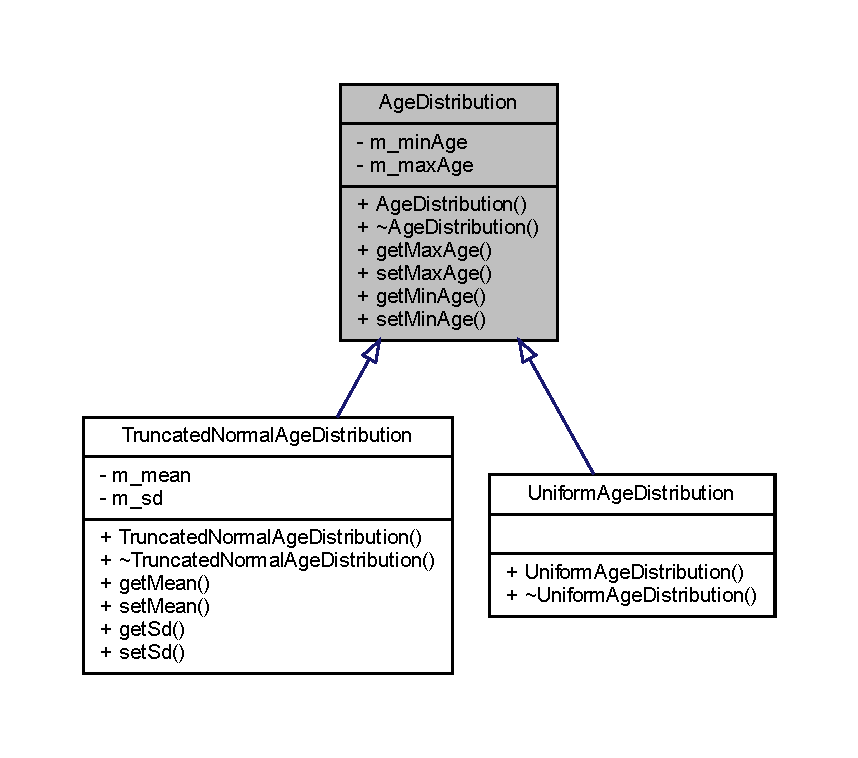
\includegraphics[width=350pt]{class_age_distribution__inherit__graph}
\end{center}
\end{figure}


Collaboration diagram for Age\+Distribution\+:\nopagebreak
\begin{figure}[H]
\begin{center}
\leavevmode
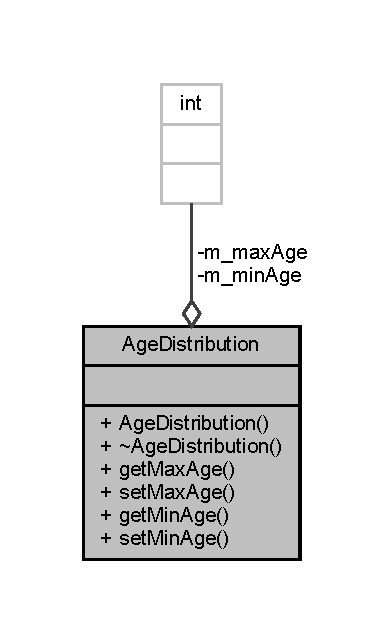
\includegraphics[width=188pt]{class_age_distribution__coll__graph}
\end{center}
\end{figure}
\doxysubsection*{Public Member Functions}
\begin{DoxyCompactItemize}
\item 
\mbox{\hyperlink{class_age_distribution_aa9eaf848716b4df66f4c2131d5a1d732}{Age\+Distribution}} (int min\+\_\+age, int max\+\_\+age)
\item 
virtual \mbox{\hyperlink{class_age_distribution_afe4ff456eada8ca46bf17c97cc2924e5}{$\sim$\+Age\+Distribution}} ()
\item 
int \mbox{\hyperlink{class_age_distribution_afe071e9af9ac30666cb350ba091327b4}{get\+Max\+Age}} () const
\item 
void \mbox{\hyperlink{class_age_distribution_a373e4c295e386eff3b31961a7a3b77e1}{set\+Max\+Age}} (int max\+Age)
\item 
int \mbox{\hyperlink{class_age_distribution_af97ddf99213aea07728813c5a658a93c}{get\+Min\+Age}} () const
\item 
void \mbox{\hyperlink{class_age_distribution_ac7ea2ef90cf3fc61d163417e6fee2abd}{set\+Min\+Age}} (int min\+Age)
\end{DoxyCompactItemize}
\doxysubsection*{Private Attributes}
\begin{DoxyCompactItemize}
\item 
int \mbox{\hyperlink{class_age_distribution_a0a0c672bcb905595bd0bc960f8cfe3a9}{m\+\_\+min\+Age}}
\item 
int \mbox{\hyperlink{class_age_distribution_a0b9a094176a3524b155edfe6849e47a3}{m\+\_\+max\+Age}}
\end{DoxyCompactItemize}


\doxysubsection{Detailed Description}
This is the base class for the age distribution among the individuals involved in a simulation. 

\doxysubsection{Constructor \& Destructor Documentation}
\mbox{\Hypertarget{class_age_distribution_aa9eaf848716b4df66f4c2131d5a1d732}\label{class_age_distribution_aa9eaf848716b4df66f4c2131d5a1d732}} 
\index{AgeDistribution@{AgeDistribution}!AgeDistribution@{AgeDistribution}}
\index{AgeDistribution@{AgeDistribution}!AgeDistribution@{AgeDistribution}}
\doxysubsubsection{\texorpdfstring{AgeDistribution()}{AgeDistribution()}}
{\footnotesize\ttfamily Age\+Distribution\+::\+Age\+Distribution (\begin{DoxyParamCaption}\item[{int}]{min\+\_\+age,  }\item[{int}]{max\+\_\+age }\end{DoxyParamCaption})}

Constructor of the class. It only sets the minimum and maximum age. 
\begin{DoxyParams}{Parameters}
{\em min\+\_\+age} & the minimum age of a person. \\
\hline
{\em max\+\_\+age} & the maximum age of a person. \\
\hline
\end{DoxyParams}
\mbox{\Hypertarget{class_age_distribution_afe4ff456eada8ca46bf17c97cc2924e5}\label{class_age_distribution_afe4ff456eada8ca46bf17c97cc2924e5}} 
\index{AgeDistribution@{AgeDistribution}!````~AgeDistribution@{$\sim$AgeDistribution}}
\index{````~AgeDistribution@{$\sim$AgeDistribution}!AgeDistribution@{AgeDistribution}}
\doxysubsubsection{\texorpdfstring{$\sim$AgeDistribution()}{~AgeDistribution()}}
{\footnotesize\ttfamily virtual Age\+Distribution\+::$\sim$\+Age\+Distribution (\begin{DoxyParamCaption}{ }\end{DoxyParamCaption})\hspace{0.3cm}{\ttfamily [virtual]}}

Destructor of the class. 

\doxysubsection{Member Function Documentation}
\mbox{\Hypertarget{class_age_distribution_afe071e9af9ac30666cb350ba091327b4}\label{class_age_distribution_afe071e9af9ac30666cb350ba091327b4}} 
\index{AgeDistribution@{AgeDistribution}!getMaxAge@{getMaxAge}}
\index{getMaxAge@{getMaxAge}!AgeDistribution@{AgeDistribution}}
\doxysubsubsection{\texorpdfstring{getMaxAge()}{getMaxAge()}}
{\footnotesize\ttfamily int Age\+Distribution\+::get\+Max\+Age (\begin{DoxyParamCaption}{ }\end{DoxyParamCaption}) const}

Returns the value of the maximum age. \begin{DoxyReturn}{Returns}
the value of the maximum age. 
\end{DoxyReturn}
\mbox{\Hypertarget{class_age_distribution_af97ddf99213aea07728813c5a658a93c}\label{class_age_distribution_af97ddf99213aea07728813c5a658a93c}} 
\index{AgeDistribution@{AgeDistribution}!getMinAge@{getMinAge}}
\index{getMinAge@{getMinAge}!AgeDistribution@{AgeDistribution}}
\doxysubsubsection{\texorpdfstring{getMinAge()}{getMinAge()}}
{\footnotesize\ttfamily int Age\+Distribution\+::get\+Min\+Age (\begin{DoxyParamCaption}{ }\end{DoxyParamCaption}) const}

Returns the value of the minimum age of a person. \begin{DoxyReturn}{Returns}
the value of the minimum age of a person. 
\end{DoxyReturn}
\mbox{\Hypertarget{class_age_distribution_a373e4c295e386eff3b31961a7a3b77e1}\label{class_age_distribution_a373e4c295e386eff3b31961a7a3b77e1}} 
\index{AgeDistribution@{AgeDistribution}!setMaxAge@{setMaxAge}}
\index{setMaxAge@{setMaxAge}!AgeDistribution@{AgeDistribution}}
\doxysubsubsection{\texorpdfstring{setMaxAge()}{setMaxAge()}}
{\footnotesize\ttfamily void Age\+Distribution\+::set\+Max\+Age (\begin{DoxyParamCaption}\item[{int}]{max\+Age }\end{DoxyParamCaption})}

Sets the maximum age. 
\begin{DoxyParams}{Parameters}
{\em max\+Age} & the value of the maximum age. \\
\hline
\end{DoxyParams}
\mbox{\Hypertarget{class_age_distribution_ac7ea2ef90cf3fc61d163417e6fee2abd}\label{class_age_distribution_ac7ea2ef90cf3fc61d163417e6fee2abd}} 
\index{AgeDistribution@{AgeDistribution}!setMinAge@{setMinAge}}
\index{setMinAge@{setMinAge}!AgeDistribution@{AgeDistribution}}
\doxysubsubsection{\texorpdfstring{setMinAge()}{setMinAge()}}
{\footnotesize\ttfamily void Age\+Distribution\+::set\+Min\+Age (\begin{DoxyParamCaption}\item[{int}]{min\+Age }\end{DoxyParamCaption})}

Sets the minimum age. 
\begin{DoxyParams}{Parameters}
{\em min\+Age} & the value of the minimum age. \\
\hline
\end{DoxyParams}


\doxysubsection{Member Data Documentation}
\mbox{\Hypertarget{class_age_distribution_a0b9a094176a3524b155edfe6849e47a3}\label{class_age_distribution_a0b9a094176a3524b155edfe6849e47a3}} 
\index{AgeDistribution@{AgeDistribution}!m\_maxAge@{m\_maxAge}}
\index{m\_maxAge@{m\_maxAge}!AgeDistribution@{AgeDistribution}}
\doxysubsubsection{\texorpdfstring{m\_maxAge}{m\_maxAge}}
{\footnotesize\ttfamily int Age\+Distribution\+::m\+\_\+max\+Age\hspace{0.3cm}{\ttfamily [private]}}

\mbox{\Hypertarget{class_age_distribution_a0a0c672bcb905595bd0bc960f8cfe3a9}\label{class_age_distribution_a0a0c672bcb905595bd0bc960f8cfe3a9}} 
\index{AgeDistribution@{AgeDistribution}!m\_minAge@{m\_minAge}}
\index{m\_minAge@{m\_minAge}!AgeDistribution@{AgeDistribution}}
\doxysubsubsection{\texorpdfstring{m\_minAge}{m\_minAge}}
{\footnotesize\ttfamily int Age\+Distribution\+::m\+\_\+min\+Age\hspace{0.3cm}{\ttfamily [private]}}



The documentation for this class was generated from the following file\+:\begin{DoxyCompactItemize}
\item 
include/\mbox{\hyperlink{_age_distribution_8h}{Age\+Distribution.\+h}}\end{DoxyCompactItemize}

\hypertarget{class_agent}{}\doxysection{Agent Class Reference}
\label{class_agent}\index{Agent@{Agent}}


{\ttfamily \#include $<$Agent.\+h$>$}



Inheritance diagram for Agent\+:\nopagebreak
\begin{figure}[H]
\begin{center}
\leavevmode
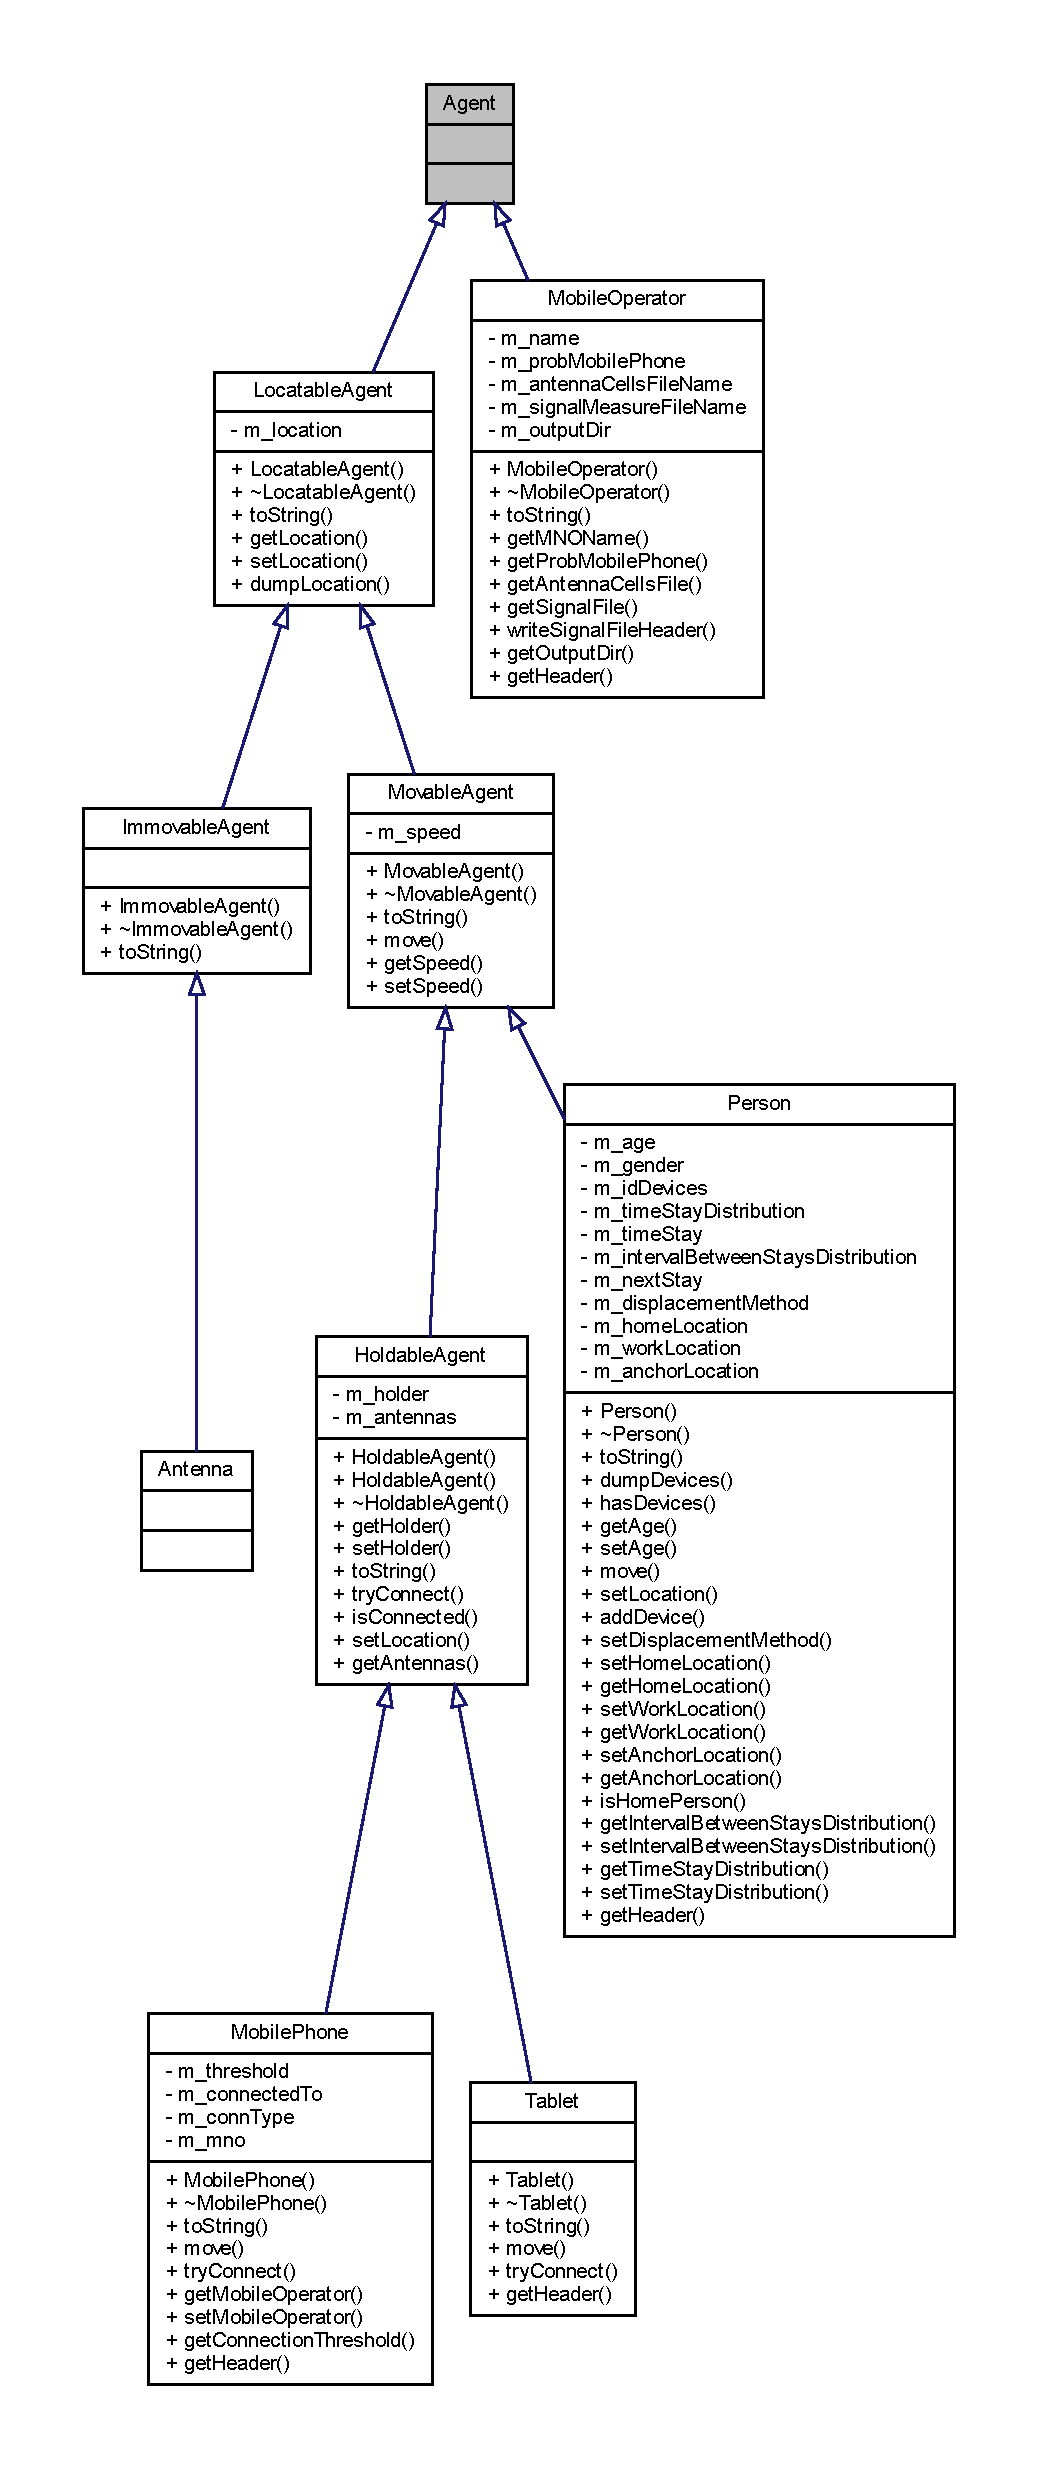
\includegraphics[height=550pt]{class_agent__inherit__graph}
\end{center}
\end{figure}


Collaboration diagram for Agent\+:\nopagebreak
\begin{figure}[H]
\begin{center}
\leavevmode
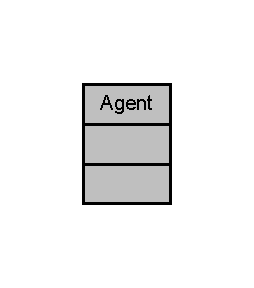
\includegraphics[height=550pt]{class_agent__coll__graph}
\end{center}
\end{figure}
\doxysubsection*{Public Member Functions}
\begin{DoxyCompactItemize}
\item 
\mbox{\hyperlink{class_agent_a24a60f1d260bf19a4f7f8a5f36881d3f}{Agent}} ()
\item 
\mbox{\hyperlink{class_agent_a0ad923f2f9966b65a5d908cb9da4217c}{Agent}} (const \mbox{\hyperlink{class_map}{Map}} $\ast$m, const unsigned long id, const \mbox{\hyperlink{class_clock}{Clock}} $\ast$clock)
\item 
virtual \mbox{\hyperlink{class_agent_a4feb26df1cf81760a0e411e393c24d4e}{$\sim$\+Agent}} ()
\item 
bool \mbox{\hyperlink{class_agent_afa2b3a408bb0694aea46fb2bb59bacf7}{operator==}} (const \mbox{\hyperlink{class_agent}{Agent}} \&a)
\item 
const virtual \mbox{\hyperlink{class_map}{Map}} $\ast$ \mbox{\hyperlink{class_agent_a4e46853ceb49887543e5688cf925cd8c}{get\+Map}} () const
\item 
const virtual \mbox{\hyperlink{class_clock}{Clock}} $\ast$ \mbox{\hyperlink{class_agent_a898fb47f4d07e3773f0ec00cf7f00a87}{get\+Clock}} () const
\item 
const virtual unsigned long \mbox{\hyperlink{class_agent_a5d2a21f30ff10676f02ad5d8c1717902}{get\+Id}} () const
\item 
const virtual string \mbox{\hyperlink{class_agent_a109600f8f99a2ad75dddc611583b050f}{to\+String}} (bool detailed=false) const =0
\end{DoxyCompactItemize}
\doxysubsection*{Private Attributes}
\begin{DoxyCompactItemize}
\item 
const \mbox{\hyperlink{class_map}{Map}} $\ast$ \mbox{\hyperlink{class_agent_ab24d62bbfc22946d0c72221c8a43f04a}{m\+\_\+map}}
\item 
const unsigned long \mbox{\hyperlink{class_agent_ad1f52e164c2a829ef4418940567d6e37}{m\+\_\+id}}
\item 
const \mbox{\hyperlink{class_clock}{Clock}} $\ast$ \mbox{\hyperlink{class_agent_a534f22ebb0573aa1d58d274632e592cf}{m\+\_\+clock}}
\end{DoxyCompactItemize}


\doxysubsection{Detailed Description}
This is an abstract class, the base class for all agents involved in a simulation. A simulation involves different types of agents implemented by specific subclasses\+: \mbox{\hyperlink{class_antenna}{Antenna}}, \mbox{\hyperlink{class_mobile_phone}{Mobile\+Phone}}, \mbox{\hyperlink{class_mobile_operator}{Mobile\+Operator}}, \mbox{\hyperlink{class_person}{Person}}. All agents are stored in a container\+: an \mbox{\hyperlink{class_agents_collection}{Agents\+Collection}} object. Some of the agents have a location on the map and they are derived from the \mbox{\hyperlink{class_locatable_agent}{Locatable\+Agent}} class that adds the location of the agent on the map. There are two types of \mbox{\hyperlink{class_locatable_agent}{Locatable\+Agent}} s\+: with a fixed location on the map during the simulation and this type of behavior is defined by the \mbox{\hyperlink{class_immovable_agent}{Immovable\+Agent}} class and with a location that can change during the simulation and they are subclasses of the \mbox{\hyperlink{class_movable_agent}{Movable\+Agent}} class. \mbox{\hyperlink{class_movable_agent}{Movable\+Agent}} objects can be either a \mbox{\hyperlink{class_person}{Person}} instance or a \mbox{\hyperlink{class_holdable_agent}{Holdable\+Agent}} subclass which means a device\+: a \mbox{\hyperlink{class_mobile_phone}{Mobile\+Phone}} object or a \mbox{\hyperlink{class_tablet}{Tablet}} object. \mbox{\hyperlink{class_locatable_agent}{Locatable\+Agent}}, \mbox{\hyperlink{class_immovable_agent}{Immovable\+Agent}}, \mbox{\hyperlink{class_holdable_agent}{Holdable\+Agent}} are abstract classes. The only classes that can be instantiated are \mbox{\hyperlink{class_antenna}{Antenna}}, \mbox{\hyperlink{class_mobile_phone}{Mobile\+Phone}}, \mbox{\hyperlink{class_mobile_operator}{Mobile\+Operator}}, \mbox{\hyperlink{class_person}{Person}}, \mbox{\hyperlink{class_tablet}{Tablet}}. An agent object has a unique id in the whole set of agents. 

\doxysubsection{Constructor \& Destructor Documentation}
\mbox{\Hypertarget{class_agent_a24a60f1d260bf19a4f7f8a5f36881d3f}\label{class_agent_a24a60f1d260bf19a4f7f8a5f36881d3f}} 
\index{Agent@{Agent}!Agent@{Agent}}
\index{Agent@{Agent}!Agent@{Agent}}
\doxysubsubsection{\texorpdfstring{Agent()}{Agent()}\hspace{0.1cm}{\footnotesize\ttfamily [1/2]}}
{\footnotesize\ttfamily Agent\+::\+Agent (\begin{DoxyParamCaption}{ }\end{DoxyParamCaption})}

Default constructor. \mbox{\Hypertarget{class_agent_a0ad923f2f9966b65a5d908cb9da4217c}\label{class_agent_a0ad923f2f9966b65a5d908cb9da4217c}} 
\index{Agent@{Agent}!Agent@{Agent}}
\index{Agent@{Agent}!Agent@{Agent}}
\doxysubsubsection{\texorpdfstring{Agent()}{Agent()}\hspace{0.1cm}{\footnotesize\ttfamily [2/2]}}
{\footnotesize\ttfamily Agent\+::\+Agent (\begin{DoxyParamCaption}\item[{const \mbox{\hyperlink{class_map}{Map}} $\ast$}]{m,  }\item[{const unsigned long}]{id,  }\item[{const \mbox{\hyperlink{class_clock}{Clock}} $\ast$}]{clock }\end{DoxyParamCaption})}

Constructor of the class. \mbox{\hyperlink{class_agent}{Agent}} is the base class for all agents used in the simulator\+: persons, antennas, mobile devices, mobile network operators. \mbox{\hyperlink{class_agent}{Agent}} is an abstract class, users should build specific subclasses. An \mbox{\hyperlink{class_agent}{Agent}} keeps a pointer to the map of the simulation, and pointer to the simulation clock. 
\begin{DoxyParams}{Parameters}
{\em m} & -\/ a pointer to the \mbox{\hyperlink{class_map}{Map}} object where the simulation take place. \\
\hline
{\em id} & -\/ the id of this agent, it uniquely identifies the agent. \\
\hline
{\em clock} & -\/ a pointer to a \mbox{\hyperlink{class_clock}{Clock}} object used by the simulator, the \mbox{\hyperlink{class_clock}{Clock}} object is the same for all agents. \\
\hline
\end{DoxyParams}
\mbox{\Hypertarget{class_agent_a4feb26df1cf81760a0e411e393c24d4e}\label{class_agent_a4feb26df1cf81760a0e411e393c24d4e}} 
\index{Agent@{Agent}!````~Agent@{$\sim$Agent}}
\index{````~Agent@{$\sim$Agent}!Agent@{Agent}}
\doxysubsubsection{\texorpdfstring{$\sim$Agent()}{~Agent()}}
{\footnotesize\ttfamily virtual Agent\+::$\sim$\+Agent (\begin{DoxyParamCaption}{ }\end{DoxyParamCaption})\hspace{0.3cm}{\ttfamily [virtual]}}

Default destructor of the class. 

\doxysubsection{Member Function Documentation}
\mbox{\Hypertarget{class_agent_a898fb47f4d07e3773f0ec00cf7f00a87}\label{class_agent_a898fb47f4d07e3773f0ec00cf7f00a87}} 
\index{Agent@{Agent}!getClock@{getClock}}
\index{getClock@{getClock}!Agent@{Agent}}
\doxysubsubsection{\texorpdfstring{getClock()}{getClock()}}
{\footnotesize\ttfamily const virtual \mbox{\hyperlink{class_clock}{Clock}}$\ast$ Agent\+::get\+Clock (\begin{DoxyParamCaption}{ }\end{DoxyParamCaption}) const\hspace{0.3cm}{\ttfamily [virtual]}}

Returns a pointer to the \mbox{\hyperlink{class_clock}{Clock}} object used for simulation. All agents use the same \mbox{\hyperlink{class_clock}{Clock}} object for a simulation. \begin{DoxyReturn}{Returns}
a pointer to the \mbox{\hyperlink{class_clock}{Clock}} object used for simulation. 
\end{DoxyReturn}
\mbox{\Hypertarget{class_agent_a5d2a21f30ff10676f02ad5d8c1717902}\label{class_agent_a5d2a21f30ff10676f02ad5d8c1717902}} 
\index{Agent@{Agent}!getId@{getId}}
\index{getId@{getId}!Agent@{Agent}}
\doxysubsubsection{\texorpdfstring{getId()}{getId()}}
{\footnotesize\ttfamily const virtual unsigned long Agent\+::get\+Id (\begin{DoxyParamCaption}{ }\end{DoxyParamCaption}) const\hspace{0.3cm}{\ttfamily [virtual]}}

Returns the id of the object. \begin{DoxyReturn}{Returns}
the id of the object. 
\end{DoxyReturn}
\mbox{\Hypertarget{class_agent_a4e46853ceb49887543e5688cf925cd8c}\label{class_agent_a4e46853ceb49887543e5688cf925cd8c}} 
\index{Agent@{Agent}!getMap@{getMap}}
\index{getMap@{getMap}!Agent@{Agent}}
\doxysubsubsection{\texorpdfstring{getMap()}{getMap()}}
{\footnotesize\ttfamily const virtual \mbox{\hyperlink{class_map}{Map}}$\ast$ Agent\+::get\+Map (\begin{DoxyParamCaption}{ }\end{DoxyParamCaption}) const\hspace{0.3cm}{\ttfamily [virtual]}}

Getter function that returns a pointer to the \mbox{\hyperlink{class_map}{Map}} object passed to the constructor when an \mbox{\hyperlink{class_agent}{Agent}} object was build. \begin{DoxyReturn}{Returns}
a pointer to the \mbox{\hyperlink{class_map}{Map}} object that was passed to the constructor. All agents use the same map for a simulation. 
\end{DoxyReturn}
\mbox{\Hypertarget{class_agent_afa2b3a408bb0694aea46fb2bb59bacf7}\label{class_agent_afa2b3a408bb0694aea46fb2bb59bacf7}} 
\index{Agent@{Agent}!operator==@{operator==}}
\index{operator==@{operator==}!Agent@{Agent}}
\doxysubsubsection{\texorpdfstring{operator==()}{operator==()}}
{\footnotesize\ttfamily bool Agent\+::operator== (\begin{DoxyParamCaption}\item[{const \mbox{\hyperlink{class_agent}{Agent}} \&}]{a }\end{DoxyParamCaption})}

The equal operator for agents. 
\begin{DoxyParams}{Parameters}
{\em a} & the object with which we test the equality. \\
\hline
\end{DoxyParams}
\begin{DoxyReturn}{Returns}
true if this object is the equal to a, false otherwise. Two objects are considered to be equal if they have the same id. 
\end{DoxyReturn}
\mbox{\Hypertarget{class_agent_a109600f8f99a2ad75dddc611583b050f}\label{class_agent_a109600f8f99a2ad75dddc611583b050f}} 
\index{Agent@{Agent}!toString@{toString}}
\index{toString@{toString}!Agent@{Agent}}
\doxysubsubsection{\texorpdfstring{toString()}{toString()}}
{\footnotesize\ttfamily const virtual string Agent\+::to\+String (\begin{DoxyParamCaption}\item[{bool}]{detailed = {\ttfamily false} }\end{DoxyParamCaption}) const\hspace{0.3cm}{\ttfamily [pure virtual]}}

Builds a string with the most relevant or all information of the class. It is useful to output the description of concrete agents to the console or to a file. Depending on the value of the {\ttfamily detailed} parameter, the string can contain only the values of the the most important members (detailed = false) or all members of the class. 
\begin{DoxyParams}{Parameters}
{\em detailed} & if true, the string will contain the values of all members (parameters) of the agent, otherwise only the most important ones are written to the output string. Each derived class will decide which are the most important members. \\
\hline
\end{DoxyParams}
\begin{DoxyReturn}{Returns}
a string object containing the most important or all members (parameters) of the agent. 
\end{DoxyReturn}


Implemented in \mbox{\hyperlink{class_antenna_afc5cb8c8fae1a251cf8c5bc6c43ff692}{Antenna}}, \mbox{\hyperlink{class_holdable_agent_a104d14d5742847a9d5fc74d18f2c1571}{Holdable\+Agent}}, \mbox{\hyperlink{class_person_a3c38c40dab5c071d20fe3aaab51975a2}{Person}}, \mbox{\hyperlink{class_mobile_operator_a46c5fc9c7a4dbea7f9d4dce7674930b6}{Mobile\+Operator}}, \mbox{\hyperlink{class_mobile_phone_a818272053e6e52ecc217dc5ee234ff69}{Mobile\+Phone}}, \mbox{\hyperlink{class_immovable_agent_a4e4851029e1e9c33baa2a193e95b8838}{Immovable\+Agent}}, \mbox{\hyperlink{class_movable_agent_a6cd9a1dc9104b5703f74785a87d2c320}{Movable\+Agent}}, \mbox{\hyperlink{class_tablet_aae4c82133cbf3e7d7e8c0cca11925159}{Tablet}}, and \mbox{\hyperlink{class_locatable_agent_ac3761e9b566f8ddcd1a663fcbf97eeac}{Locatable\+Agent}}.



\doxysubsection{Member Data Documentation}
\mbox{\Hypertarget{class_agent_a534f22ebb0573aa1d58d274632e592cf}\label{class_agent_a534f22ebb0573aa1d58d274632e592cf}} 
\index{Agent@{Agent}!m\_clock@{m\_clock}}
\index{m\_clock@{m\_clock}!Agent@{Agent}}
\doxysubsubsection{\texorpdfstring{m\_clock}{m\_clock}}
{\footnotesize\ttfamily const \mbox{\hyperlink{class_clock}{Clock}}$\ast$ Agent\+::m\+\_\+clock\hspace{0.3cm}{\ttfamily [private]}}

\mbox{\Hypertarget{class_agent_ad1f52e164c2a829ef4418940567d6e37}\label{class_agent_ad1f52e164c2a829ef4418940567d6e37}} 
\index{Agent@{Agent}!m\_id@{m\_id}}
\index{m\_id@{m\_id}!Agent@{Agent}}
\doxysubsubsection{\texorpdfstring{m\_id}{m\_id}}
{\footnotesize\ttfamily const unsigned long Agent\+::m\+\_\+id\hspace{0.3cm}{\ttfamily [private]}}

\mbox{\Hypertarget{class_agent_ab24d62bbfc22946d0c72221c8a43f04a}\label{class_agent_ab24d62bbfc22946d0c72221c8a43f04a}} 
\index{Agent@{Agent}!m\_map@{m\_map}}
\index{m\_map@{m\_map}!Agent@{Agent}}
\doxysubsubsection{\texorpdfstring{m\_map}{m\_map}}
{\footnotesize\ttfamily const \mbox{\hyperlink{class_map}{Map}}$\ast$ Agent\+::m\+\_\+map\hspace{0.3cm}{\ttfamily [private]}}



The documentation for this class was generated from the following file\+:\begin{DoxyCompactItemize}
\item 
include/agent/\mbox{\hyperlink{_agent_8h}{Agent.\+h}}\end{DoxyCompactItemize}

\hypertarget{class_agents_collection}{}\doxysection{Agents\+Collection Class Reference}
\label{class_agents_collection}\index{AgentsCollection@{AgentsCollection}}


{\ttfamily \#include $<$Agents\+Collection.\+h$>$}



Collaboration diagram for Agents\+Collection\+:\nopagebreak
\begin{figure}[H]
\begin{center}
\leavevmode
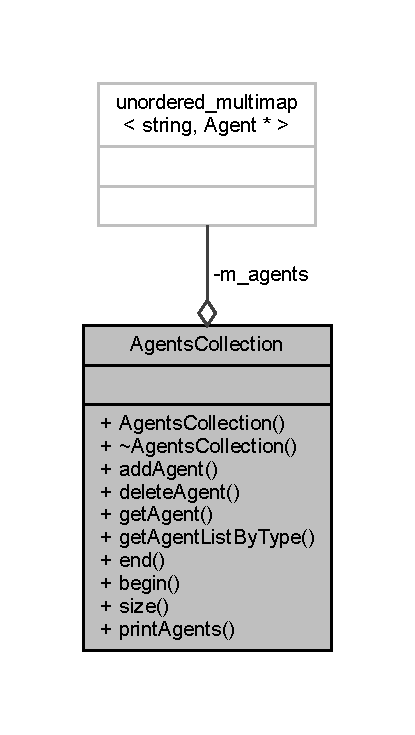
\includegraphics[width=199pt]{class_agents_collection__coll__graph}
\end{center}
\end{figure}
\doxysubsection*{Public Member Functions}
\begin{DoxyCompactItemize}
\item 
\mbox{\hyperlink{class_agents_collection_a866b0ed56c0109e82bc7c839de0a3267}{Agents\+Collection}} ()
\item 
virtual \mbox{\hyperlink{class_agents_collection_a8a58eb1f8a45cc4d1c0e04dd912dbae0}{$\sim$\+Agents\+Collection}} ()
\item 
void \mbox{\hyperlink{class_agents_collection_acf8ed7260a13c2dc710faffe399695b2}{add\+Agent}} (\mbox{\hyperlink{class_agent}{Agent}} $\ast$ag)
\item 
\mbox{\hyperlink{class_agent}{Agent}} $\ast$ \mbox{\hyperlink{class_agents_collection_aed912dae777e6a0e37137c4de4b02cc9}{delete\+Agent}} (\mbox{\hyperlink{class_agent}{Agent}} $\ast$ag)
\item 
\mbox{\hyperlink{class_agent}{Agent}} $\ast$ \mbox{\hyperlink{class_agents_collection_a4b6b57c50d715edb3404520cfdb32688}{get\+Agent}} (const unsigned long id) const
\item 
pair$<$ \mbox{\hyperlink{_agents_collection_8h_afde47bc45d604b8b8c72755072376679}{um\+\_\+iterator}}, \mbox{\hyperlink{_agents_collection_8h_afde47bc45d604b8b8c72755072376679}{um\+\_\+iterator}} $>$ \mbox{\hyperlink{class_agents_collection_a4ab0c8e86e6f6ebceb12bd2bd8f9f758}{get\+Agent\+List\+By\+Type}} (const string \&agent\+Type)
\item 
\mbox{\hyperlink{_agents_collection_8h_afde47bc45d604b8b8c72755072376679}{um\+\_\+iterator}} \mbox{\hyperlink{class_agents_collection_afc61b751cf3387ab4a1bf0dfbc29cb82}{end}} ()
\item 
\mbox{\hyperlink{_agents_collection_8h_afde47bc45d604b8b8c72755072376679}{um\+\_\+iterator}} \mbox{\hyperlink{class_agents_collection_abc1d6593a3ed1c1c7b2d31b7efec8db8}{begin}} ()
\item 
unsigned long \mbox{\hyperlink{class_agents_collection_a3226f7eb58b11623bdb353d8938f60d3}{size}} ()
\item 
void \mbox{\hyperlink{class_agents_collection_a193faf9793030715e8edeb65137156e9}{print\+Agents}} ()
\end{DoxyCompactItemize}
\doxysubsection*{Private Attributes}
\begin{DoxyCompactItemize}
\item 
unordered\+\_\+multimap$<$ string, \mbox{\hyperlink{class_agent}{Agent}} $\ast$ $>$ \mbox{\hyperlink{class_agents_collection_a35a5728b0e0108c2f37897720c904dd1}{m\+\_\+agents}}
\end{DoxyCompactItemize}


\doxysubsection{Detailed Description}
This is actually a container for all the agents used for simulation. An agent could be an object of one the the derived classes of \mbox{\hyperlink{class_agent}{Agent}}. The Agents are kept in an unordered\+\_\+multimap as pairs of $<$string, Agent$\ast$$>$ where the first element of the pair is the name of the concrete agent (a person, a mobile device, an antenna, a mobile network operator, etc.) and the second element is a pointer to the actual object (agent). 

\doxysubsection{Constructor \& Destructor Documentation}
\mbox{\Hypertarget{class_agents_collection_a866b0ed56c0109e82bc7c839de0a3267}\label{class_agents_collection_a866b0ed56c0109e82bc7c839de0a3267}} 
\index{AgentsCollection@{AgentsCollection}!AgentsCollection@{AgentsCollection}}
\index{AgentsCollection@{AgentsCollection}!AgentsCollection@{AgentsCollection}}
\doxysubsubsection{\texorpdfstring{AgentsCollection()}{AgentsCollection()}}
{\footnotesize\ttfamily Agents\+Collection\+::\+Agents\+Collection (\begin{DoxyParamCaption}{ }\end{DoxyParamCaption})}

The default constructor of the class. \mbox{\Hypertarget{class_agents_collection_a8a58eb1f8a45cc4d1c0e04dd912dbae0}\label{class_agents_collection_a8a58eb1f8a45cc4d1c0e04dd912dbae0}} 
\index{AgentsCollection@{AgentsCollection}!````~AgentsCollection@{$\sim$AgentsCollection}}
\index{````~AgentsCollection@{$\sim$AgentsCollection}!AgentsCollection@{AgentsCollection}}
\doxysubsubsection{\texorpdfstring{$\sim$AgentsCollection()}{~AgentsCollection()}}
{\footnotesize\ttfamily virtual Agents\+Collection\+::$\sim$\+Agents\+Collection (\begin{DoxyParamCaption}{ }\end{DoxyParamCaption})\hspace{0.3cm}{\ttfamily [virtual]}}

Default destructor\+: it iterates through the collection of agents and frees the memory allocated for each agent in the collection. 

\doxysubsection{Member Function Documentation}
\mbox{\Hypertarget{class_agents_collection_acf8ed7260a13c2dc710faffe399695b2}\label{class_agents_collection_acf8ed7260a13c2dc710faffe399695b2}} 
\index{AgentsCollection@{AgentsCollection}!addAgent@{addAgent}}
\index{addAgent@{addAgent}!AgentsCollection@{AgentsCollection}}
\doxysubsubsection{\texorpdfstring{addAgent()}{addAgent()}}
{\footnotesize\ttfamily void Agents\+Collection\+::add\+Agent (\begin{DoxyParamCaption}\item[{\mbox{\hyperlink{class_agent}{Agent}} $\ast$}]{ag }\end{DoxyParamCaption})}

Adds a new \mbox{\hyperlink{class_agent}{Agent}} object to the collection. For performance reasons the \mbox{\hyperlink{class_agents_collection}{Agents\+Collection}} class keep only a pointer to actual agents (objects). 
\begin{DoxyParams}{Parameters}
{\em ag} & a pointer to the object (one of the derived classes of the \mbox{\hyperlink{class_agent}{Agent}}) to be added to the collection. \\
\hline
\end{DoxyParams}
\mbox{\Hypertarget{class_agents_collection_abc1d6593a3ed1c1c7b2d31b7efec8db8}\label{class_agents_collection_abc1d6593a3ed1c1c7b2d31b7efec8db8}} 
\index{AgentsCollection@{AgentsCollection}!begin@{begin}}
\index{begin@{begin}!AgentsCollection@{AgentsCollection}}
\doxysubsubsection{\texorpdfstring{begin()}{begin()}}
{\footnotesize\ttfamily \mbox{\hyperlink{_agents_collection_8h_afde47bc45d604b8b8c72755072376679}{um\+\_\+iterator}} Agents\+Collection\+::begin (\begin{DoxyParamCaption}{ }\end{DoxyParamCaption})}

Iterator to the first object of the container. \begin{DoxyReturn}{Returns}
a random access iterator pointing to the first element (agent) in the container. If the container is empty, the returned iterator value shall not be dereferenced. 
\end{DoxyReturn}
\mbox{\Hypertarget{class_agents_collection_aed912dae777e6a0e37137c4de4b02cc9}\label{class_agents_collection_aed912dae777e6a0e37137c4de4b02cc9}} 
\index{AgentsCollection@{AgentsCollection}!deleteAgent@{deleteAgent}}
\index{deleteAgent@{deleteAgent}!AgentsCollection@{AgentsCollection}}
\doxysubsubsection{\texorpdfstring{deleteAgent()}{deleteAgent()}}
{\footnotesize\ttfamily \mbox{\hyperlink{class_agent}{Agent}}$\ast$ Agents\+Collection\+::delete\+Agent (\begin{DoxyParamCaption}\item[{\mbox{\hyperlink{class_agent}{Agent}} $\ast$}]{ag }\end{DoxyParamCaption})}

Removes an object from the collection. 
\begin{DoxyParams}{Parameters}
{\em ag} & a pointer to the object to be removed from the collection. \\
\hline
\end{DoxyParams}
\begin{DoxyReturn}{Returns}
a pointer to the object removed from the collection 
\end{DoxyReturn}
\mbox{\Hypertarget{class_agents_collection_afc61b751cf3387ab4a1bf0dfbc29cb82}\label{class_agents_collection_afc61b751cf3387ab4a1bf0dfbc29cb82}} 
\index{AgentsCollection@{AgentsCollection}!end@{end}}
\index{end@{end}!AgentsCollection@{AgentsCollection}}
\doxysubsubsection{\texorpdfstring{end()}{end()}}
{\footnotesize\ttfamily \mbox{\hyperlink{_agents_collection_8h_afde47bc45d604b8b8c72755072376679}{um\+\_\+iterator}} Agents\+Collection\+::end (\begin{DoxyParamCaption}{ }\end{DoxyParamCaption})}

Iterator to the past-\/the-\/end object of the collection. It does not point to any agent, and thus shall not be dereferenced. \begin{DoxyReturn}{Returns}
an iterator referring to the past-\/the-\/end element in the agents container. If the container is empty, this function returns the same as \mbox{\hyperlink{class_agents_collection_abc1d6593a3ed1c1c7b2d31b7efec8db8}{Agents\+Collection\+::begin()}}. 
\end{DoxyReturn}
\mbox{\Hypertarget{class_agents_collection_a4b6b57c50d715edb3404520cfdb32688}\label{class_agents_collection_a4b6b57c50d715edb3404520cfdb32688}} 
\index{AgentsCollection@{AgentsCollection}!getAgent@{getAgent}}
\index{getAgent@{getAgent}!AgentsCollection@{AgentsCollection}}
\doxysubsubsection{\texorpdfstring{getAgent()}{getAgent()}}
{\footnotesize\ttfamily \mbox{\hyperlink{class_agent}{Agent}}$\ast$ Agents\+Collection\+::get\+Agent (\begin{DoxyParamCaption}\item[{const unsigned long}]{id }\end{DoxyParamCaption}) const}

Returns a pointer to an agent from the collection. The agent/object is identified by its id which is unique throughout the collection. 
\begin{DoxyParams}{Parameters}
{\em id} & the id of the agent to be returned. \\
\hline
\end{DoxyParams}
\begin{DoxyReturn}{Returns}
a pointer to the agent with the id equals to the parameter {\ttfamily id}. If there is no agent with the provided id, this method returns {\ttfamily nullptr}. 
\end{DoxyReturn}
\mbox{\Hypertarget{class_agents_collection_a4ab0c8e86e6f6ebceb12bd2bd8f9f758}\label{class_agents_collection_a4ab0c8e86e6f6ebceb12bd2bd8f9f758}} 
\index{AgentsCollection@{AgentsCollection}!getAgentListByType@{getAgentListByType}}
\index{getAgentListByType@{getAgentListByType}!AgentsCollection@{AgentsCollection}}
\doxysubsubsection{\texorpdfstring{getAgentListByType()}{getAgentListByType()}}
{\footnotesize\ttfamily pair$<$\mbox{\hyperlink{_agents_collection_8h_afde47bc45d604b8b8c72755072376679}{um\+\_\+iterator}}, \mbox{\hyperlink{_agents_collection_8h_afde47bc45d604b8b8c72755072376679}{um\+\_\+iterator}}$>$ Agents\+Collection\+::get\+Agent\+List\+By\+Type (\begin{DoxyParamCaption}\item[{const string \&}]{agent\+Type }\end{DoxyParamCaption})}

This method is used to retrieve a subset of agents with a certain type\+: persons, mobile phones etc. 
\begin{DoxyParams}{Parameters}
{\em agent\+Type} & is the name of the class of agents that the user wants to retrieve from the collection of all agents. \\
\hline
\end{DoxyParams}
\begin{DoxyReturn}{Returns}
a std\+::pair of iterators of type unordered\+\_\+multimap$<$string, Agent$\ast$$>$\+::iterator that can be used to iterate through to subset of the agents. 
\end{DoxyReturn}
\mbox{\Hypertarget{class_agents_collection_a193faf9793030715e8edeb65137156e9}\label{class_agents_collection_a193faf9793030715e8edeb65137156e9}} 
\index{AgentsCollection@{AgentsCollection}!printAgents@{printAgents}}
\index{printAgents@{printAgents}!AgentsCollection@{AgentsCollection}}
\doxysubsubsection{\texorpdfstring{printAgents()}{printAgents()}}
{\footnotesize\ttfamily void Agents\+Collection\+::print\+Agents (\begin{DoxyParamCaption}{ }\end{DoxyParamCaption})}

Prints out all agents in the collection calling \mbox{\hyperlink{namespaceutils_a38505d06d647192484ebea7d650bd92f}{to\+String()}} method for each agent. \mbox{\Hypertarget{class_agents_collection_a3226f7eb58b11623bdb353d8938f60d3}\label{class_agents_collection_a3226f7eb58b11623bdb353d8938f60d3}} 
\index{AgentsCollection@{AgentsCollection}!size@{size}}
\index{size@{size}!AgentsCollection@{AgentsCollection}}
\doxysubsubsection{\texorpdfstring{size()}{size()}}
{\footnotesize\ttfamily unsigned long Agents\+Collection\+::size (\begin{DoxyParamCaption}{ }\end{DoxyParamCaption})}

Returns the number of elements in the container. \begin{DoxyReturn}{Returns}
the number of elements in the container. This is the number of actual objects held in the container,which is not necessarily equal to its storage capacity. 
\end{DoxyReturn}


\doxysubsection{Member Data Documentation}
\mbox{\Hypertarget{class_agents_collection_a35a5728b0e0108c2f37897720c904dd1}\label{class_agents_collection_a35a5728b0e0108c2f37897720c904dd1}} 
\index{AgentsCollection@{AgentsCollection}!m\_agents@{m\_agents}}
\index{m\_agents@{m\_agents}!AgentsCollection@{AgentsCollection}}
\doxysubsubsection{\texorpdfstring{m\_agents}{m\_agents}}
{\footnotesize\ttfamily unordered\+\_\+multimap$<$string, \mbox{\hyperlink{class_agent}{Agent}}$\ast$$>$ Agents\+Collection\+::m\+\_\+agents\hspace{0.3cm}{\ttfamily [private]}}



The documentation for this class was generated from the following file\+:\begin{DoxyCompactItemize}
\item 
include/agent/\mbox{\hyperlink{_agents_collection_8h}{Agents\+Collection.\+h}}\end{DoxyCompactItemize}

\hypertarget{class_antenna}{}\doxysection{Antenna Class Reference}
\label{class_antenna}\index{Antenna@{Antenna}}


{\ttfamily \#include $<$Antenna.\+h$>$}



Inheritance diagram for Antenna\+:\nopagebreak
\begin{figure}[H]
\begin{center}
\leavevmode
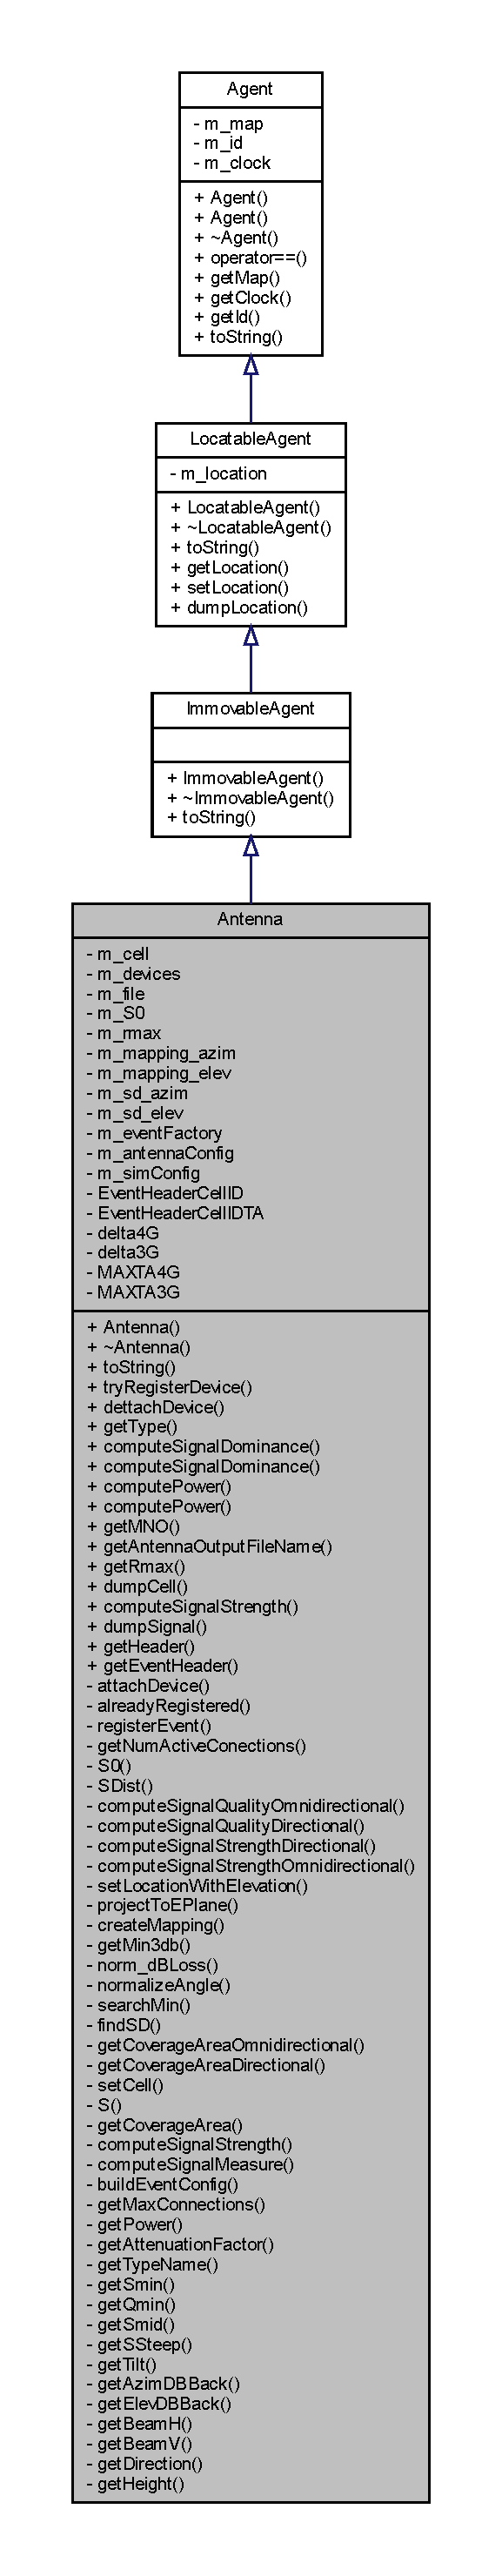
\includegraphics[height=550pt]{class_antenna__inherit__graph}
\end{center}
\end{figure}


Collaboration diagram for Antenna\+:\nopagebreak
\begin{figure}[H]
\begin{center}
\leavevmode
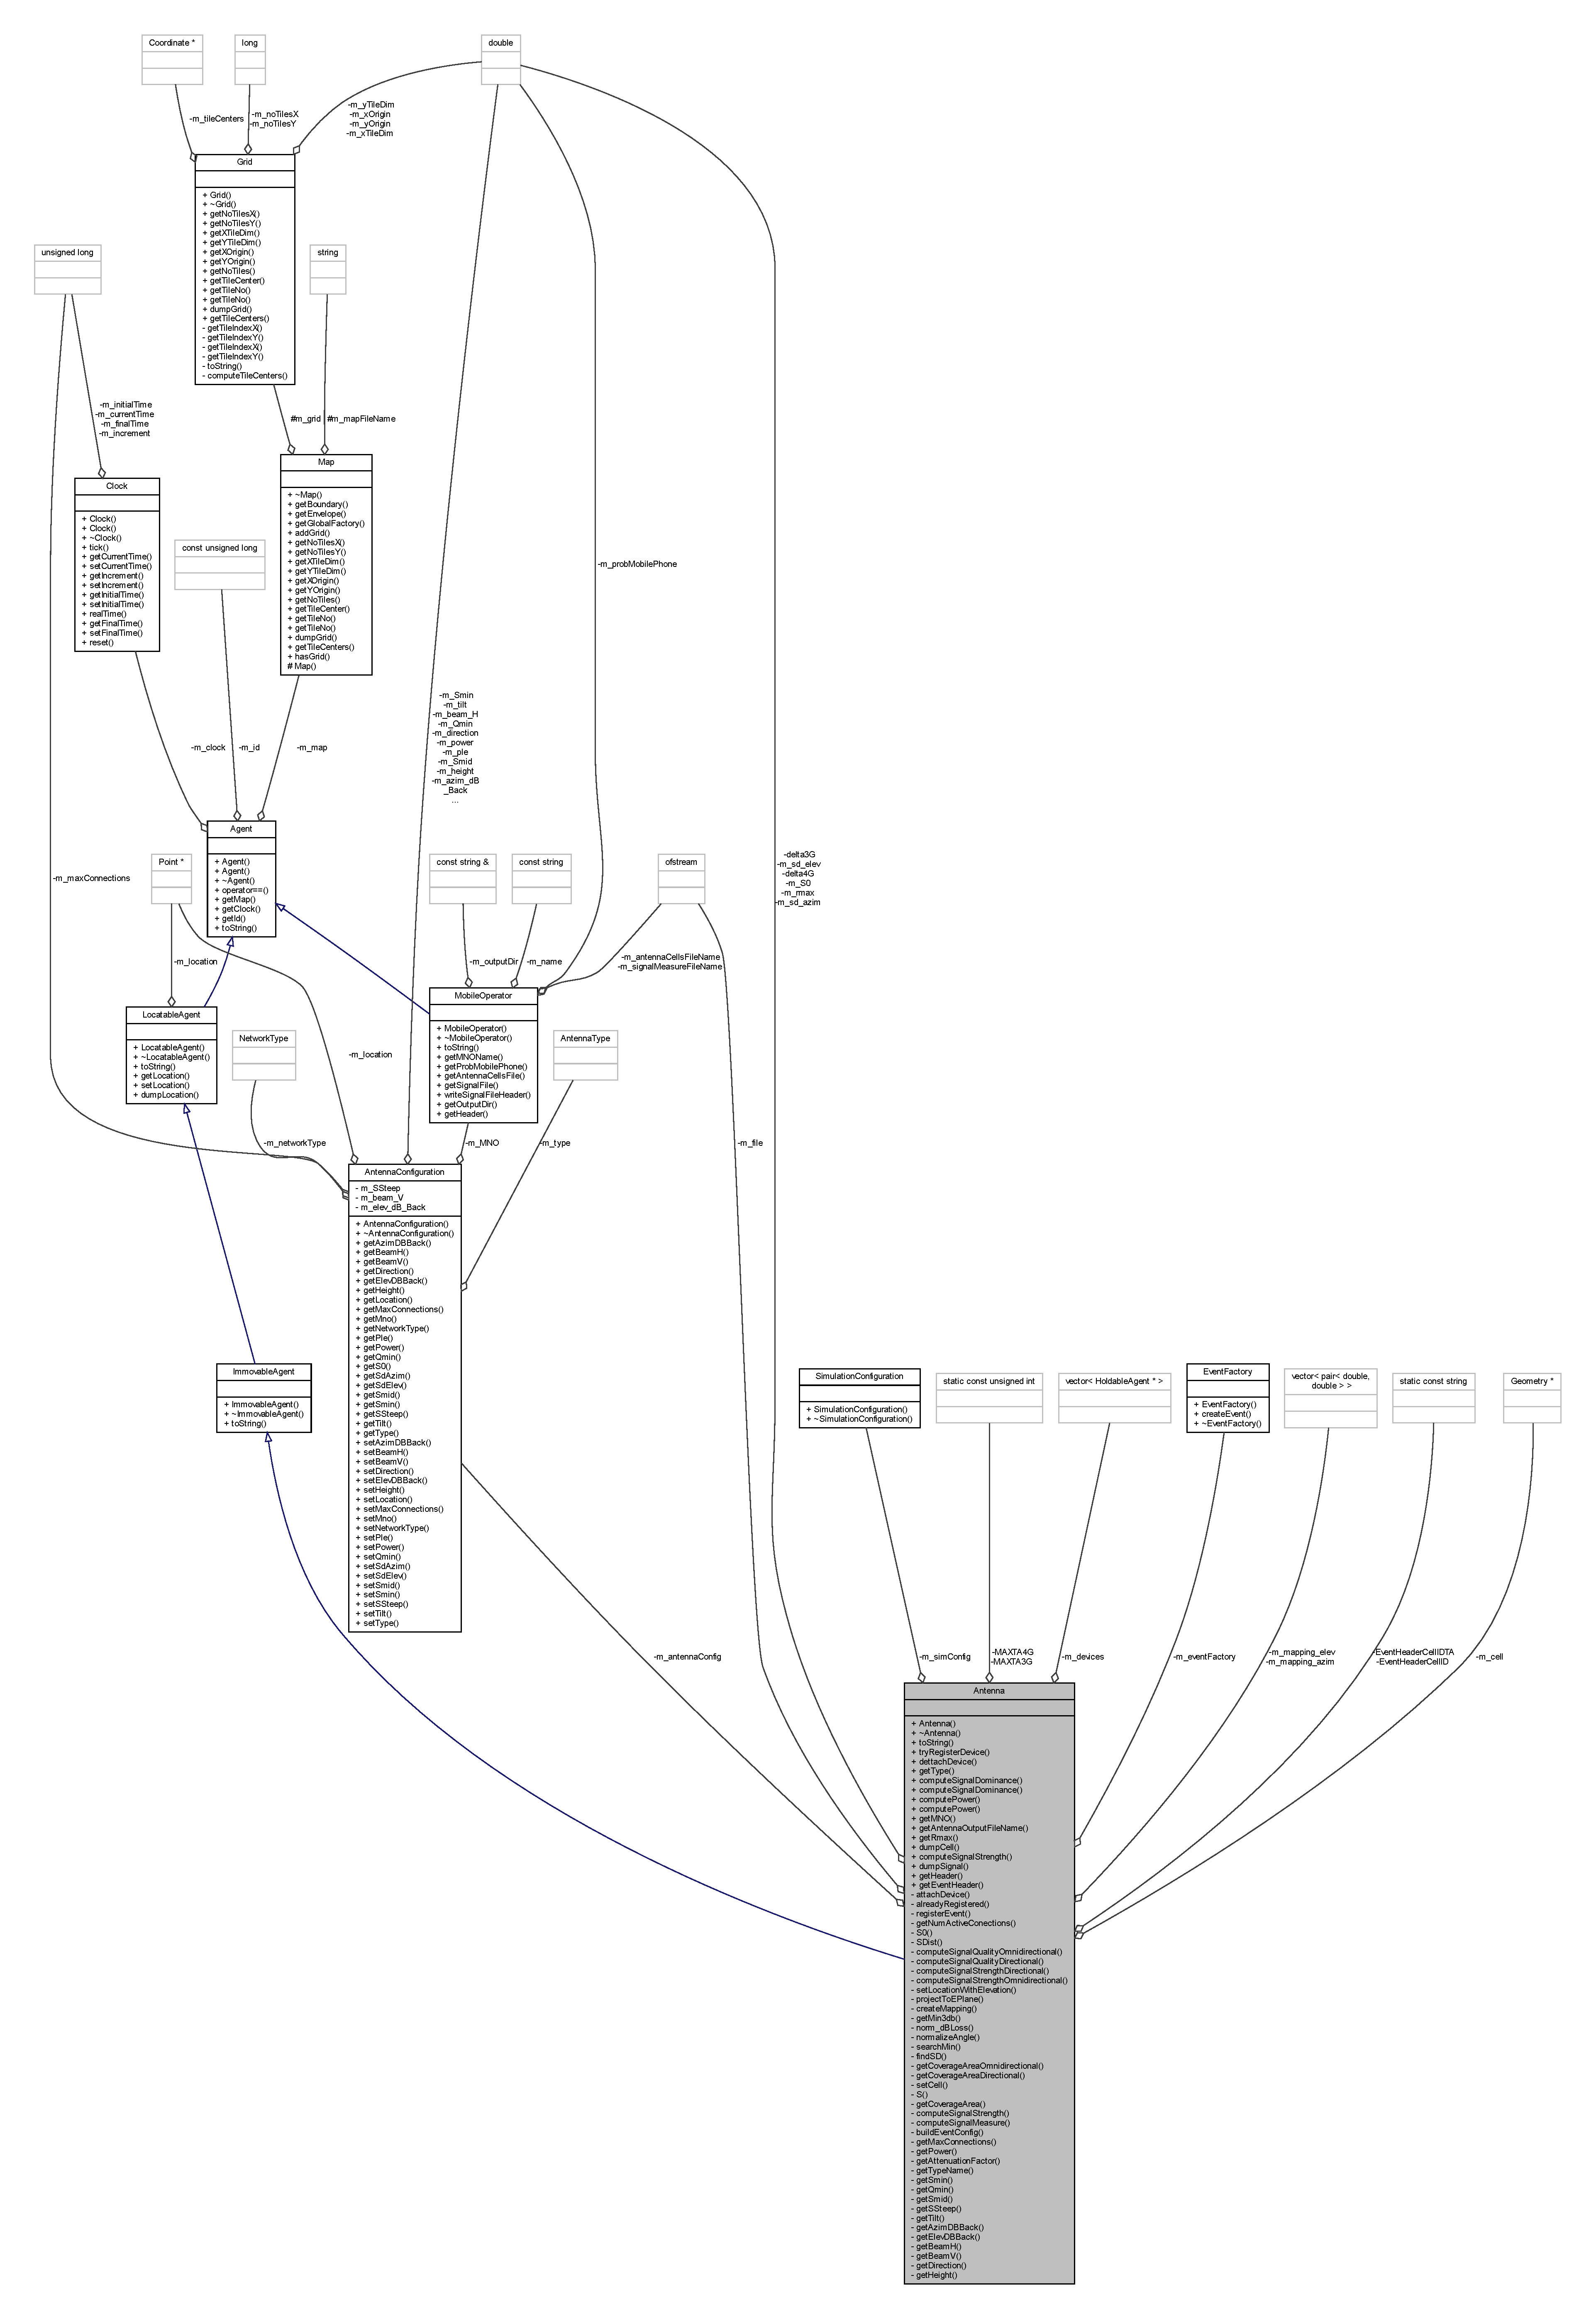
\includegraphics[width=350pt]{class_antenna__coll__graph}
\end{center}
\end{figure}
\doxysubsection*{Public Member Functions}
\begin{DoxyCompactItemize}
\item 
\mbox{\hyperlink{class_antenna_a3ffd61a2c9634c3cb6449c6b1e2d0ff8}{Antenna}} (const unsigned long id, \mbox{\hyperlink{class_simulation_configuration}{Simulation\+Configuration}} $\ast$sc, \mbox{\hyperlink{class_antenna_configuration}{Antenna\+Configuration}} ac, \mbox{\hyperlink{class_event_factory}{Event\+Factory}} $\ast$factory)
\item 
virtual \mbox{\hyperlink{class_antenna_ad7b98073b970db5d6bc83c5c5961fe44}{$\sim$\+Antenna}} ()
\item 
const string \mbox{\hyperlink{class_antenna_afc5cb8c8fae1a251cf8c5bc6c43ff692}{to\+String}} (bool detailed=false) const override
\item 
bool \mbox{\hyperlink{class_antenna_a4455f5c804e1ea520dd849dc9fd7b0b4}{try\+Register\+Device}} (\mbox{\hyperlink{class_holdable_agent}{Holdable\+Agent}} $\ast$device)
\item 
void \mbox{\hyperlink{class_antenna_a983a0784315567c2ab6ac1820cf558c5}{dettach\+Device}} (\mbox{\hyperlink{class_holdable_agent}{Holdable\+Agent}} $\ast$device)
\item 
\mbox{\hyperlink{_antenna_type_8h_a7b678b5cb9dedc607131200119d96b16}{Antenna\+Type}} \mbox{\hyperlink{class_antenna_adf45a8b339956741bf8dcb5361f5f249}{get\+Type}} () const
\item 
double \mbox{\hyperlink{class_antenna_ad5e95089dd452dfee52194d2955a7b76}{compute\+Signal\+Dominance}} (const Point $\ast$p) const
\item 
double \mbox{\hyperlink{class_antenna_aadb456a9cce4ed0c7b6e4d15a084f359}{compute\+Signal\+Dominance}} (const Coordinate c) const
\item 
double \mbox{\hyperlink{class_antenna_a7caa8004be14f97db64fdf7ae46d6c97}{compute\+Power}} (const Point $\ast$p) const
\item 
double \mbox{\hyperlink{class_antenna_a0192376f8702c5300fe1f13ce267b305}{compute\+Power}} (const Coordinate c) const
\item 
\mbox{\hyperlink{class_mobile_operator}{Mobile\+Operator}} $\ast$ \mbox{\hyperlink{class_antenna_abfbb4a654f73fe0c3a30f50777f79349}{get\+M\+NO}} () const
\item 
string \mbox{\hyperlink{class_antenna_a7a3919b137b91c1f8f13d620bc7657ed}{get\+Antenna\+Output\+File\+Name}} () const
\item 
double \mbox{\hyperlink{class_antenna_adf33d1b0be85f95c543a31dc1b3159f5}{get\+Rmax}} () const
\item 
string \mbox{\hyperlink{class_antenna_a8ed18205ff7c675868090e4c80454c2c}{dump\+Cell}} () const
\item 
double \mbox{\hyperlink{class_antenna_a228297a3cb00c11fab97d615b4817656}{compute\+Signal\+Strength}} (const Point $\ast$p) const
\item 
void \mbox{\hyperlink{class_antenna_ad78e7561bf98d891262e6436cd3e1df7}{dump\+Signal}} () const
\end{DoxyCompactItemize}
\doxysubsection*{Static Public Member Functions}
\begin{DoxyCompactItemize}
\item 
static const string \mbox{\hyperlink{class_antenna_a9d56406fd66fc0835c373ea342dee7af}{get\+Header}} (bool detailed=false)
\item 
static string \mbox{\hyperlink{class_antenna_aef8e1cda793839c25ccee7888db37943}{get\+Event\+Header}} (\mbox{\hyperlink{_event_type_8h_a2628ea8d12e8b2563c32f05dc7fff6fa}{Event\+Type}} ev\+Type)
\end{DoxyCompactItemize}
\doxysubsection*{Private Member Functions}
\begin{DoxyCompactItemize}
\item 
void \mbox{\hyperlink{class_antenna_a9c804d991a545157feb066761b6a69ef}{attach\+Device}} (\mbox{\hyperlink{class_holdable_agent}{Holdable\+Agent}} $\ast$device)
\item 
bool \mbox{\hyperlink{class_antenna_af4fb83843393bf36bdcaefae5b5dd0dd}{already\+Registered}} (\mbox{\hyperlink{class_holdable_agent}{Holdable\+Agent}} $\ast$ag)
\item 
void \mbox{\hyperlink{class_antenna_aa931ec91c960c6d5704d4e25cf17229f}{register\+Event}} (\mbox{\hyperlink{class_event}{Event}} $\ast$ev, Point $\ast$evt\+Location)
\item 
unsigned long \mbox{\hyperlink{class_antenna_a86c5c094ab6ea432609afa00f3a8080a}{get\+Num\+Active\+Conections}} ()
\item 
double \mbox{\hyperlink{class_antenna_a033246c50bec80123860154a949620c7}{S0}} () const
\item 
double \mbox{\hyperlink{class_antenna_ae60ab40ded94be407c3b7455f4e886fe}{S\+Dist}} (double dist) const
\item 
double \mbox{\hyperlink{class_antenna_a036e212fda08a9fc5215732378fc4fbd}{compute\+Signal\+Quality\+Omnidirectional}} (const Coordinate c) const
\item 
double \mbox{\hyperlink{class_antenna_a0bba3b0a586d5dc36397c2b9887cd42b}{compute\+Signal\+Quality\+Directional}} (const Coordinate c) const
\item 
double \mbox{\hyperlink{class_antenna_a38bb70c5ca249773512186c34792b43a}{compute\+Signal\+Strength\+Directional}} (const Coordinate c) const
\item 
double \mbox{\hyperlink{class_antenna_a26077f4061413733cedf9253ecc8686f}{compute\+Signal\+Strength\+Omnidirectional}} (const Coordinate c) const
\item 
void \mbox{\hyperlink{class_antenna_a4b1d0ae147826e553a044fd481d6c7e0}{set\+Location\+With\+Elevation}} ()
\item 
double \mbox{\hyperlink{class_antenna_a298c80a54828c8f13d584e8e382145a5}{project\+To\+E\+Plane}} (double b, double c, double beta) const
\item 
vector$<$ pair$<$ double, double $>$ $>$ \mbox{\hyperlink{class_antenna_afe86e36673d4b28713f983cc63d89e1b}{create\+Mapping}} (double db\+Back) const
\item 
double \mbox{\hyperlink{class_antenna_a1c6126c232ee496b9b693fc20e4892f5}{get\+Min3db}} (double sd, double db\+Back) const
\item 
double \mbox{\hyperlink{class_antenna_a8270b1a03b61af1e048650e00a129b93}{norm\+\_\+d\+B\+Loss}} (double angle, double db\+Back, double sd) const
\item 
double \mbox{\hyperlink{class_antenna_a353ae3aafbc75033c30fb96004c2b73f}{normalize\+Angle}} (double angle) const
\item 
double \mbox{\hyperlink{class_antenna_a48ef89b0d1bd313bae4ca863da1cc77e}{search\+Min}} (double dg, vector$<$ pair$<$ double, double $>$$>$ \+\_\+3d\+B\+Degrees) const
\item 
double \mbox{\hyperlink{class_antenna_affb34fcbb958e09bd48a2c3069e06ac8}{find\+SD}} (double beam\+Width, double db\+Back, vector$<$ pair$<$ double, double $>$$>$ \&mapping) const
\item 
Geometry $\ast$ \mbox{\hyperlink{class_antenna_a24f459b9915a64fe140af16a2970a7e7}{get\+Coverage\+Area\+Omnidirectional}} () const
\item 
Geometry $\ast$ \mbox{\hyperlink{class_antenna_afa9076da40bdebf6b80c582657e6ce48}{get\+Coverage\+Area\+Directional}} () const
\item 
void \mbox{\hyperlink{class_antenna_ae44355f1ba577a3129788b507c217dba}{set\+Cell}} (\mbox{\hyperlink{class_holdable_agent_ae2c334b004d7b9c5a999cf2618e4e518}{Holdable\+Agent\+::\+C\+O\+N\+N\+E\+C\+T\+I\+O\+N\+\_\+\+T\+Y\+PE}} handover\+Mechanism)
\item 
double \mbox{\hyperlink{class_antenna_a5715c4100035c58d63b7c9a0195748fe}{S}} (double dist) const
\item 
Geometry $\ast$ \mbox{\hyperlink{class_antenna_a5f94dd903add1b59957514887388bd52}{get\+Coverage\+Area}} ()
\item 
double \mbox{\hyperlink{class_antenna_ac33fe5654d4e3307a4c1c155b0f89128}{compute\+Signal\+Strength}} (const Coordinate c) const
\item 
double \mbox{\hyperlink{class_antenna_a2fab50e7dbe01acec58d7fe89798e9b6}{compute\+Signal\+Measure}} (\mbox{\hyperlink{class_holdable_agent_ae2c334b004d7b9c5a999cf2618e4e518}{Holdable\+Agent\+::\+C\+O\+N\+N\+E\+C\+T\+I\+O\+N\+\_\+\+T\+Y\+PE}} handover\+Type, const Coordinate c) const
\item 
\mbox{\hyperlink{class_event_config}{Event\+Config}} $\ast$ \mbox{\hyperlink{class_antenna_aa657d5e0bb29cf0d44ebb614e56fed2a}{build\+Event\+Config}} (\mbox{\hyperlink{_event_type_8h_a2628ea8d12e8b2563c32f05dc7fff6fa}{Event\+Type}} ev\+Type, \mbox{\hyperlink{_event_code_8h_a080ee5c80bcb8b9f3fda41b5e4eb0ef8}{Event\+Code}} code, \mbox{\hyperlink{class_holdable_agent}{Holdable\+Agent}} $\ast$device)
\item 
unsigned long \mbox{\hyperlink{class_antenna_ac7d42215283cd7d4dc16d449f61af91d}{get\+Max\+Connections}} () const
\item 
double \mbox{\hyperlink{class_antenna_afca01d00c8e393ee911f1e9240b51d2e}{get\+Power}} () const
\item 
double \mbox{\hyperlink{class_antenna_a9551ed22d25c51210913de4a3074d9eb}{get\+Attenuation\+Factor}} () const
\item 
string \mbox{\hyperlink{class_antenna_a40941201e4b272c4b9593e05aa1ac38e}{get\+Type\+Name}} () const
\item 
double \mbox{\hyperlink{class_antenna_a1955f59f9d3b20ffd8e79f4893bf2e61}{get\+Smin}} () const
\item 
double \mbox{\hyperlink{class_antenna_a67b245a43ba9d94ba4b7d3fdace7b73c}{get\+Qmin}} () const
\item 
double \mbox{\hyperlink{class_antenna_acfaf47d35cc742e76522ea31a8b01578}{get\+Smid}} () const
\item 
double \mbox{\hyperlink{class_antenna_a096deca0fe8497c0fe53539ae80f2db5}{get\+S\+Steep}} () const
\item 
double \mbox{\hyperlink{class_antenna_a9feaa77de0a608a7f59eb0854ae746a7}{get\+Tilt}} () const
\item 
double \mbox{\hyperlink{class_antenna_a1354b8be09c0985c3710a8c91ee11dd6}{get\+Azim\+D\+B\+Back}} () const
\item 
double \mbox{\hyperlink{class_antenna_ae4abdaeb483291d0e11cbcc393a0f6a3}{get\+Elev\+D\+B\+Back}} () const
\item 
double \mbox{\hyperlink{class_antenna_a5c1f0eaf769dae9172f450dbe8708be6}{get\+BeamH}} () const
\item 
double \mbox{\hyperlink{class_antenna_af3ce30dbc386b7d97e4ddc4c13356b85}{get\+BeamV}} () const
\item 
double \mbox{\hyperlink{class_antenna_a76d97c4f0e2b8ad00c1dbedc1710673c}{get\+Direction}} () const
\item 
double \mbox{\hyperlink{class_antenna_a04be1246cff927d077d62a82ed7eb25e}{get\+Height}} () const
\end{DoxyCompactItemize}
\doxysubsection*{Private Attributes}
\begin{DoxyCompactItemize}
\item 
Geometry $\ast$ \mbox{\hyperlink{class_antenna_addbe8e6ae7a8bad737339d23bc2abbba}{m\+\_\+cell}}
\item 
vector$<$ \mbox{\hyperlink{class_holdable_agent}{Holdable\+Agent}} $\ast$ $>$ \mbox{\hyperlink{class_antenna_a2d0f7032eb1d8cc6c02b1dd64bc59856}{m\+\_\+devices}}
\item 
ofstream \mbox{\hyperlink{class_antenna_a06824840191e96b19eb224d53e08d3ec}{m\+\_\+file}}
\item 
double \mbox{\hyperlink{class_antenna_a65bdd3ec77862b9427df42ae74dc54e4}{m\+\_\+\+S0}}
\item 
double \mbox{\hyperlink{class_antenna_a7b8fda5c94e7cf03c14a0fe5447e5d46}{m\+\_\+rmax}}
\item 
vector$<$ pair$<$ double, double $>$ $>$ \mbox{\hyperlink{class_antenna_a0d4e25b246a30e3e6fdb303bed85e7da}{m\+\_\+mapping\+\_\+azim}}
\item 
vector$<$ pair$<$ double, double $>$ $>$ \mbox{\hyperlink{class_antenna_a71b55ca74697d064e231829343209fec}{m\+\_\+mapping\+\_\+elev}}
\item 
double \mbox{\hyperlink{class_antenna_af9ed0b78826b52bd60c497eb7f87be3d}{m\+\_\+sd\+\_\+azim}}
\item 
double \mbox{\hyperlink{class_antenna_aeb2ce4a95682b9ecff1395dfa857c089}{m\+\_\+sd\+\_\+elev}}
\item 
\mbox{\hyperlink{class_event_factory}{Event\+Factory}} $\ast$ \mbox{\hyperlink{class_antenna_a7044507cdeb0d10a92c61adaf243f5b5}{m\+\_\+event\+Factory}}
\item 
\mbox{\hyperlink{class_antenna_configuration}{Antenna\+Configuration}} \mbox{\hyperlink{class_antenna_a766312d18a74270713fc69cf55b2578b}{m\+\_\+antenna\+Config}}
\item 
\mbox{\hyperlink{class_simulation_configuration}{Simulation\+Configuration}} $\ast$ \mbox{\hyperlink{class_antenna_aa6a04536655e94183422cf1937d2897e}{m\+\_\+sim\+Config}}
\end{DoxyCompactItemize}
\doxysubsection*{Static Private Attributes}
\begin{DoxyCompactItemize}
\item 
static const string \mbox{\hyperlink{class_antenna_aff940632ce74397357cb5400c0c47599}{Event\+Header\+Cell\+ID}}
\item 
static const string \mbox{\hyperlink{class_antenna_a1a3e590ebd908d331e725c865cc629dd}{Event\+Header\+Cell\+I\+D\+TA}}
\item 
static const double \mbox{\hyperlink{class_antenna_a929c2809d9dff6252471abfd4872ef5b}{delta4G}}
\item 
static const double \mbox{\hyperlink{class_antenna_a77a68a26f1e7844c358960da0e432c79}{delta3G}}
\item 
static const unsigned int \mbox{\hyperlink{class_antenna_a8986d0863767e330a12751aad05d9c25}{M\+A\+X\+T\+A4G}}
\item 
static const unsigned int \mbox{\hyperlink{class_antenna_a29191686e9d14f85bd84c8e43c2237fb}{M\+A\+X\+T\+A3G}}
\end{DoxyCompactItemize}


\doxysubsection{Detailed Description}
This class simulates an antenna (a base transceiver station, or shortly B\+TS) of the mobile phone network. It has a fixed location on the map and registers the events generated by the interaction with the mobile devices in a .csv file. Each antenna has its own file where it saves the events and the name of this file. The name of this file is composed by concatenating \char`\"{}\+Antenna\char`\"{}, its id, \char`\"{}\+\_\+\+M\+N\+O\+\_\+\char`\"{} and the M\+NO name read from the configuration file. The are two types of antennas\+: omnidirectional and directional. An omnidirectional antenna emits homogeneous signal in all directions. We model the signal using two measures\+: \begin{DoxyItemize}
\item the signal strength \item the signal dominance\end{DoxyItemize}
The signal strength at distance {\itshape r} from the antenna\textquotesingle{}s location is given by \+:

R\+S\+S(r) = 30 + 10 log10(\+P) -\/ 10 gamma log10(r) where {\itshape P} is the power of the antenna in Watts and {\itshape gamma} is the attenuation factor of the signal (also called the path loss exponent),

while the signal dominance is given by\+:

S\+D\+M(r) = 1/(1 + exp (-\/Ssteep ( R\+S\+S(r) -\/ Smid)))

where {\itshape Ssteep} and {\itshape Smid} are parameters that should be given in the configuration file.

For a complete definition of the signal dominance one can consult\+: Tennekes M, Gootzen Y\+A\+PM, Shah SH (2020) A Bayesian approach to location estimation of mobile devices from mobile network operator data. Research Report, Statistics Netherlands (C\+BS).

A directional antenna has a specific signal emission pattern and one can find a description of it in the work mentioned above. 

\doxysubsection{Constructor \& Destructor Documentation}
\mbox{\Hypertarget{class_antenna_a3ffd61a2c9634c3cb6449c6b1e2d0ff8}\label{class_antenna_a3ffd61a2c9634c3cb6449c6b1e2d0ff8}} 
\index{Antenna@{Antenna}!Antenna@{Antenna}}
\index{Antenna@{Antenna}!Antenna@{Antenna}}
\doxysubsubsection{\texorpdfstring{Antenna()}{Antenna()}}
{\footnotesize\ttfamily Antenna\+::\+Antenna (\begin{DoxyParamCaption}\item[{const unsigned long}]{id,  }\item[{\mbox{\hyperlink{class_simulation_configuration}{Simulation\+Configuration}} $\ast$}]{sc,  }\item[{\mbox{\hyperlink{class_antenna_configuration}{Antenna\+Configuration}}}]{ac,  }\item[{\mbox{\hyperlink{class_event_factory}{Event\+Factory}} $\ast$}]{factory }\end{DoxyParamCaption})\hspace{0.3cm}{\ttfamily [explicit]}}

This is the constructor of the class. It is used to build antenna objects. 
\begin{DoxyParams}{Parameters}
{\em id} & the ID of this object, which is unique throughout the entire collection of agents. \\
\hline
{\em sc} & a pointer to a \mbox{\hyperlink{class_simulation_configuration}{Simulation\+Configuration}} object that contains the parameters of the simulation read from the configuration file. \\
\hline
{\em ac} & an \mbox{\hyperlink{class_antenna_configuration}{Antenna\+Configuration}} object that contains all the technical parameters of an antenna, together with its type. These parameters are specified in the antennas\textquotesingle{} configuration file. \\
\hline
{\em factory} & a pointer to an \mbox{\hyperlink{class_event_factory}{Event\+Factory}} object used to create \mbox{\hyperlink{class_event}{Event}} objects according to the event type specified in the simulation configuration file. \\
\hline
\end{DoxyParams}
\mbox{\Hypertarget{class_antenna_ad7b98073b970db5d6bc83c5c5961fe44}\label{class_antenna_ad7b98073b970db5d6bc83c5c5961fe44}} 
\index{Antenna@{Antenna}!````~Antenna@{$\sim$Antenna}}
\index{````~Antenna@{$\sim$Antenna}!Antenna@{Antenna}}
\doxysubsubsection{\texorpdfstring{$\sim$Antenna()}{~Antenna()}}
{\footnotesize\ttfamily virtual Antenna\+::$\sim$\+Antenna (\begin{DoxyParamCaption}{ }\end{DoxyParamCaption})\hspace{0.3cm}{\ttfamily [virtual]}}

Destructor of the class. It closes the file where the \mbox{\hyperlink{class_antenna}{Antenna}} dumps the registered events during the simulation. 

\doxysubsection{Member Function Documentation}
\mbox{\Hypertarget{class_antenna_af4fb83843393bf36bdcaefae5b5dd0dd}\label{class_antenna_af4fb83843393bf36bdcaefae5b5dd0dd}} 
\index{Antenna@{Antenna}!alreadyRegistered@{alreadyRegistered}}
\index{alreadyRegistered@{alreadyRegistered}!Antenna@{Antenna}}
\doxysubsubsection{\texorpdfstring{alreadyRegistered()}{alreadyRegistered()}}
{\footnotesize\ttfamily bool Antenna\+::already\+Registered (\begin{DoxyParamCaption}\item[{\mbox{\hyperlink{class_holdable_agent}{Holdable\+Agent}} $\ast$}]{ag }\end{DoxyParamCaption})\hspace{0.3cm}{\ttfamily [private]}}

\mbox{\Hypertarget{class_antenna_a9c804d991a545157feb066761b6a69ef}\label{class_antenna_a9c804d991a545157feb066761b6a69ef}} 
\index{Antenna@{Antenna}!attachDevice@{attachDevice}}
\index{attachDevice@{attachDevice}!Antenna@{Antenna}}
\doxysubsubsection{\texorpdfstring{attachDevice()}{attachDevice()}}
{\footnotesize\ttfamily void Antenna\+::attach\+Device (\begin{DoxyParamCaption}\item[{\mbox{\hyperlink{class_holdable_agent}{Holdable\+Agent}} $\ast$}]{device }\end{DoxyParamCaption})\hspace{0.3cm}{\ttfamily [private]}}

\mbox{\Hypertarget{class_antenna_aa657d5e0bb29cf0d44ebb614e56fed2a}\label{class_antenna_aa657d5e0bb29cf0d44ebb614e56fed2a}} 
\index{Antenna@{Antenna}!buildEventConfig@{buildEventConfig}}
\index{buildEventConfig@{buildEventConfig}!Antenna@{Antenna}}
\doxysubsubsection{\texorpdfstring{buildEventConfig()}{buildEventConfig()}}
{\footnotesize\ttfamily \mbox{\hyperlink{class_event_config}{Event\+Config}}$\ast$ Antenna\+::build\+Event\+Config (\begin{DoxyParamCaption}\item[{\mbox{\hyperlink{_event_type_8h_a2628ea8d12e8b2563c32f05dc7fff6fa}{Event\+Type}}}]{ev\+Type,  }\item[{\mbox{\hyperlink{_event_code_8h_a080ee5c80bcb8b9f3fda41b5e4eb0ef8}{Event\+Code}}}]{code,  }\item[{\mbox{\hyperlink{class_holdable_agent}{Holdable\+Agent}} $\ast$}]{device }\end{DoxyParamCaption})\hspace{0.3cm}{\ttfamily [private]}}

\mbox{\Hypertarget{class_antenna_a0192376f8702c5300fe1f13ce267b305}\label{class_antenna_a0192376f8702c5300fe1f13ce267b305}} 
\index{Antenna@{Antenna}!computePower@{computePower}}
\index{computePower@{computePower}!Antenna@{Antenna}}
\doxysubsubsection{\texorpdfstring{computePower()}{computePower()}\hspace{0.1cm}{\footnotesize\ttfamily [1/2]}}
{\footnotesize\ttfamily double Antenna\+::compute\+Power (\begin{DoxyParamCaption}\item[{const Coordinate}]{c }\end{DoxyParamCaption}) const}

Computes the signal power given by this \mbox{\hyperlink{class_antenna}{Antenna}} object in a certain location. 
\begin{DoxyParams}{Parameters}
{\em c} & the coordinates of the location where we want to compute the signal power. \\
\hline
\end{DoxyParams}
\begin{DoxyReturn}{Returns}
the power of the signal in the location given by Coordinate c. 
\end{DoxyReturn}
\mbox{\Hypertarget{class_antenna_a7caa8004be14f97db64fdf7ae46d6c97}\label{class_antenna_a7caa8004be14f97db64fdf7ae46d6c97}} 
\index{Antenna@{Antenna}!computePower@{computePower}}
\index{computePower@{computePower}!Antenna@{Antenna}}
\doxysubsubsection{\texorpdfstring{computePower()}{computePower()}\hspace{0.1cm}{\footnotesize\ttfamily [2/2]}}
{\footnotesize\ttfamily double Antenna\+::compute\+Power (\begin{DoxyParamCaption}\item[{const Point $\ast$}]{p }\end{DoxyParamCaption}) const}

Computes the signal power given by this \mbox{\hyperlink{class_antenna}{Antenna}} object in a certain location. 
\begin{DoxyParams}{Parameters}
{\em p} & a pointer to a Point object giving the location where we want to compute the signal power. \\
\hline
\end{DoxyParams}
\begin{DoxyReturn}{Returns}
the power of the signal in the location given by Point p. 
\end{DoxyReturn}
\mbox{\Hypertarget{class_antenna_aadb456a9cce4ed0c7b6e4d15a084f359}\label{class_antenna_aadb456a9cce4ed0c7b6e4d15a084f359}} 
\index{Antenna@{Antenna}!computeSignalDominance@{computeSignalDominance}}
\index{computeSignalDominance@{computeSignalDominance}!Antenna@{Antenna}}
\doxysubsubsection{\texorpdfstring{computeSignalDominance()}{computeSignalDominance()}\hspace{0.1cm}{\footnotesize\ttfamily [1/2]}}
{\footnotesize\ttfamily double Antenna\+::compute\+Signal\+Dominance (\begin{DoxyParamCaption}\item[{const Coordinate}]{c }\end{DoxyParamCaption}) const}

Computes the signal dominance given by this \mbox{\hyperlink{class_antenna}{Antenna}} object in a certain location. 
\begin{DoxyParams}{Parameters}
{\em c} & the coordinates of the location where we want to compute the signal dominance. \\
\hline
\end{DoxyParams}
\begin{DoxyReturn}{Returns}
the value of the signal dominance. 
\end{DoxyReturn}
\mbox{\Hypertarget{class_antenna_ad5e95089dd452dfee52194d2955a7b76}\label{class_antenna_ad5e95089dd452dfee52194d2955a7b76}} 
\index{Antenna@{Antenna}!computeSignalDominance@{computeSignalDominance}}
\index{computeSignalDominance@{computeSignalDominance}!Antenna@{Antenna}}
\doxysubsubsection{\texorpdfstring{computeSignalDominance()}{computeSignalDominance()}\hspace{0.1cm}{\footnotesize\ttfamily [2/2]}}
{\footnotesize\ttfamily double Antenna\+::compute\+Signal\+Dominance (\begin{DoxyParamCaption}\item[{const Point $\ast$}]{p }\end{DoxyParamCaption}) const}

Computes the signal dominance given by this \mbox{\hyperlink{class_antenna}{Antenna}} object in a certain location. 
\begin{DoxyParams}{Parameters}
{\em p} & a pointer to a Point object giving the location where we want to compute the signal dominance. \\
\hline
\end{DoxyParams}
\begin{DoxyReturn}{Returns}
the value of the signal dominance. 
\end{DoxyReturn}
\mbox{\Hypertarget{class_antenna_a2fab50e7dbe01acec58d7fe89798e9b6}\label{class_antenna_a2fab50e7dbe01acec58d7fe89798e9b6}} 
\index{Antenna@{Antenna}!computeSignalMeasure@{computeSignalMeasure}}
\index{computeSignalMeasure@{computeSignalMeasure}!Antenna@{Antenna}}
\doxysubsubsection{\texorpdfstring{computeSignalMeasure()}{computeSignalMeasure()}}
{\footnotesize\ttfamily double Antenna\+::compute\+Signal\+Measure (\begin{DoxyParamCaption}\item[{\mbox{\hyperlink{class_holdable_agent_ae2c334b004d7b9c5a999cf2618e4e518}{Holdable\+Agent\+::\+C\+O\+N\+N\+E\+C\+T\+I\+O\+N\+\_\+\+T\+Y\+PE}}}]{handover\+Type,  }\item[{const Coordinate}]{c }\end{DoxyParamCaption}) const\hspace{0.3cm}{\ttfamily [private]}}

\mbox{\Hypertarget{class_antenna_a0bba3b0a586d5dc36397c2b9887cd42b}\label{class_antenna_a0bba3b0a586d5dc36397c2b9887cd42b}} 
\index{Antenna@{Antenna}!computeSignalQualityDirectional@{computeSignalQualityDirectional}}
\index{computeSignalQualityDirectional@{computeSignalQualityDirectional}!Antenna@{Antenna}}
\doxysubsubsection{\texorpdfstring{computeSignalQualityDirectional()}{computeSignalQualityDirectional()}}
{\footnotesize\ttfamily double Antenna\+::compute\+Signal\+Quality\+Directional (\begin{DoxyParamCaption}\item[{const Coordinate}]{c }\end{DoxyParamCaption}) const\hspace{0.3cm}{\ttfamily [private]}}

\mbox{\Hypertarget{class_antenna_a036e212fda08a9fc5215732378fc4fbd}\label{class_antenna_a036e212fda08a9fc5215732378fc4fbd}} 
\index{Antenna@{Antenna}!computeSignalQualityOmnidirectional@{computeSignalQualityOmnidirectional}}
\index{computeSignalQualityOmnidirectional@{computeSignalQualityOmnidirectional}!Antenna@{Antenna}}
\doxysubsubsection{\texorpdfstring{computeSignalQualityOmnidirectional()}{computeSignalQualityOmnidirectional()}}
{\footnotesize\ttfamily double Antenna\+::compute\+Signal\+Quality\+Omnidirectional (\begin{DoxyParamCaption}\item[{const Coordinate}]{c }\end{DoxyParamCaption}) const\hspace{0.3cm}{\ttfamily [private]}}

\mbox{\Hypertarget{class_antenna_ac33fe5654d4e3307a4c1c155b0f89128}\label{class_antenna_ac33fe5654d4e3307a4c1c155b0f89128}} 
\index{Antenna@{Antenna}!computeSignalStrength@{computeSignalStrength}}
\index{computeSignalStrength@{computeSignalStrength}!Antenna@{Antenna}}
\doxysubsubsection{\texorpdfstring{computeSignalStrength()}{computeSignalStrength()}\hspace{0.1cm}{\footnotesize\ttfamily [1/2]}}
{\footnotesize\ttfamily double Antenna\+::compute\+Signal\+Strength (\begin{DoxyParamCaption}\item[{const Coordinate}]{c }\end{DoxyParamCaption}) const\hspace{0.3cm}{\ttfamily [private]}}

\mbox{\Hypertarget{class_antenna_a228297a3cb00c11fab97d615b4817656}\label{class_antenna_a228297a3cb00c11fab97d615b4817656}} 
\index{Antenna@{Antenna}!computeSignalStrength@{computeSignalStrength}}
\index{computeSignalStrength@{computeSignalStrength}!Antenna@{Antenna}}
\doxysubsubsection{\texorpdfstring{computeSignalStrength()}{computeSignalStrength()}\hspace{0.1cm}{\footnotesize\ttfamily [2/2]}}
{\footnotesize\ttfamily double Antenna\+::compute\+Signal\+Strength (\begin{DoxyParamCaption}\item[{const Point $\ast$}]{p }\end{DoxyParamCaption}) const}

Computes the signal strength given by this \mbox{\hyperlink{class_antenna}{Antenna}} object in a certain location. 
\begin{DoxyParams}{Parameters}
{\em p} & a pointer to a Point object giving the location where we want to compute the signal strength. \\
\hline
\end{DoxyParams}
\begin{DoxyReturn}{Returns}
the value of the signal strength. 
\end{DoxyReturn}
\mbox{\Hypertarget{class_antenna_a38bb70c5ca249773512186c34792b43a}\label{class_antenna_a38bb70c5ca249773512186c34792b43a}} 
\index{Antenna@{Antenna}!computeSignalStrengthDirectional@{computeSignalStrengthDirectional}}
\index{computeSignalStrengthDirectional@{computeSignalStrengthDirectional}!Antenna@{Antenna}}
\doxysubsubsection{\texorpdfstring{computeSignalStrengthDirectional()}{computeSignalStrengthDirectional()}}
{\footnotesize\ttfamily double Antenna\+::compute\+Signal\+Strength\+Directional (\begin{DoxyParamCaption}\item[{const Coordinate}]{c }\end{DoxyParamCaption}) const\hspace{0.3cm}{\ttfamily [private]}}

\mbox{\Hypertarget{class_antenna_a26077f4061413733cedf9253ecc8686f}\label{class_antenna_a26077f4061413733cedf9253ecc8686f}} 
\index{Antenna@{Antenna}!computeSignalStrengthOmnidirectional@{computeSignalStrengthOmnidirectional}}
\index{computeSignalStrengthOmnidirectional@{computeSignalStrengthOmnidirectional}!Antenna@{Antenna}}
\doxysubsubsection{\texorpdfstring{computeSignalStrengthOmnidirectional()}{computeSignalStrengthOmnidirectional()}}
{\footnotesize\ttfamily double Antenna\+::compute\+Signal\+Strength\+Omnidirectional (\begin{DoxyParamCaption}\item[{const Coordinate}]{c }\end{DoxyParamCaption}) const\hspace{0.3cm}{\ttfamily [private]}}

\mbox{\Hypertarget{class_antenna_afe86e36673d4b28713f983cc63d89e1b}\label{class_antenna_afe86e36673d4b28713f983cc63d89e1b}} 
\index{Antenna@{Antenna}!createMapping@{createMapping}}
\index{createMapping@{createMapping}!Antenna@{Antenna}}
\doxysubsubsection{\texorpdfstring{createMapping()}{createMapping()}}
{\footnotesize\ttfamily vector$<$pair$<$double, double$>$ $>$ Antenna\+::create\+Mapping (\begin{DoxyParamCaption}\item[{double}]{db\+Back }\end{DoxyParamCaption}) const\hspace{0.3cm}{\ttfamily [private]}}

\mbox{\Hypertarget{class_antenna_a983a0784315567c2ab6ac1820cf558c5}\label{class_antenna_a983a0784315567c2ab6ac1820cf558c5}} 
\index{Antenna@{Antenna}!dettachDevice@{dettachDevice}}
\index{dettachDevice@{dettachDevice}!Antenna@{Antenna}}
\doxysubsubsection{\texorpdfstring{dettachDevice()}{dettachDevice()}}
{\footnotesize\ttfamily void Antenna\+::dettach\+Device (\begin{DoxyParamCaption}\item[{\mbox{\hyperlink{class_holdable_agent}{Holdable\+Agent}} $\ast$}]{device }\end{DoxyParamCaption})}

Disconnects a mobile device from the antenna and outputs a detach event (code Event\+Type\+::\+D\+E\+T\+A\+C\+H\+\_\+\+D\+E\+V\+I\+CE) in the events file. This happens when the device the device has moved far enough away from the antenna so that it can no longer receive a signal that can be useful. Internally, the mobile device is removed from the list of the connected mobile devices. 
\begin{DoxyParams}{Parameters}
{\em device} & a pointer to the device to be disconnected/detached from this antenna. \\
\hline
\end{DoxyParams}
\mbox{\Hypertarget{class_antenna_a8ed18205ff7c675868090e4c80454c2c}\label{class_antenna_a8ed18205ff7c675868090e4c80454c2c}} 
\index{Antenna@{Antenna}!dumpCell@{dumpCell}}
\index{dumpCell@{dumpCell}!Antenna@{Antenna}}
\doxysubsubsection{\texorpdfstring{dumpCell()}{dumpCell()}}
{\footnotesize\ttfamily string Antenna\+::dump\+Cell (\begin{DoxyParamCaption}{ }\end{DoxyParamCaption}) const}

Builds a {\ttfamily wkt} string that represents the coverage area of this antenna. This area is a circle with the radius given by \mbox{\hyperlink{class_antenna_adf33d1b0be85f95c543a31dc1b3159f5}{get\+Rmax()}} in case the antenna in omnidirectional. In case of a directional antenna this coverage area is computed as a Polygon made up of points on segments starting from the antenna location where the signal strength/dominance drop below the minimum allowable limit. The segments covers the trigonometric circle, with a direction angle from the vertical axis starting from 0 and going to 2 $\ast$ PI, with a step of 2P\+I/100. \begin{DoxyReturn}{Returns}
a {\ttfamily wkt} string object that represents the coverage area of this antenna. 
\end{DoxyReturn}
\mbox{\Hypertarget{class_antenna_ad78e7561bf98d891262e6436cd3e1df7}\label{class_antenna_ad78e7561bf98d891262e6436cd3e1df7}} 
\index{Antenna@{Antenna}!dumpSignal@{dumpSignal}}
\index{dumpSignal@{dumpSignal}!Antenna@{Antenna}}
\doxysubsubsection{\texorpdfstring{dumpSignal()}{dumpSignal()}}
{\footnotesize\ttfamily void Antenna\+::dump\+Signal (\begin{DoxyParamCaption}{ }\end{DoxyParamCaption}) const}

Writes the values of the signal strength/dominance in a .csv file. These values are computed in the center of each tile covering the map. The name of the file is obtained from the \mbox{\hyperlink{class_mobile_operator}{Mobile\+Operator}} object that owns this antenna, by calling get\+Signal\+File(). The strength or dominance is chosen according to the handover mechanism specified in the simulation configuration file. \mbox{\Hypertarget{class_antenna_affb34fcbb958e09bd48a2c3069e06ac8}\label{class_antenna_affb34fcbb958e09bd48a2c3069e06ac8}} 
\index{Antenna@{Antenna}!findSD@{findSD}}
\index{findSD@{findSD}!Antenna@{Antenna}}
\doxysubsubsection{\texorpdfstring{findSD()}{findSD()}}
{\footnotesize\ttfamily double Antenna\+::find\+SD (\begin{DoxyParamCaption}\item[{double}]{beam\+Width,  }\item[{double}]{db\+Back,  }\item[{vector$<$ pair$<$ double, double $>$$>$ \&}]{mapping }\end{DoxyParamCaption}) const\hspace{0.3cm}{\ttfamily [private]}}

\mbox{\Hypertarget{class_antenna_a7a3919b137b91c1f8f13d620bc7657ed}\label{class_antenna_a7a3919b137b91c1f8f13d620bc7657ed}} 
\index{Antenna@{Antenna}!getAntennaOutputFileName@{getAntennaOutputFileName}}
\index{getAntennaOutputFileName@{getAntennaOutputFileName}!Antenna@{Antenna}}
\doxysubsubsection{\texorpdfstring{getAntennaOutputFileName()}{getAntennaOutputFileName()}}
{\footnotesize\ttfamily string Antenna\+::get\+Antenna\+Output\+File\+Name (\begin{DoxyParamCaption}{ }\end{DoxyParamCaption}) const}

Builds the name of the output file where the events registered by this \mbox{\hyperlink{class_antenna}{Antenna}} object during a simulation are saved. The name is built by by concatenating \char`\"{}\+Antenna\char`\"{}, its id, \char`\"{}\+\_\+\+M\+N\+O\+\_\+\char`\"{} and the M\+NO name read from the configuration file \begin{DoxyReturn}{Returns}
the name of the output file where the events registered by this \mbox{\hyperlink{class_antenna}{Antenna}} object during a simulation are saved. 
\end{DoxyReturn}
\mbox{\Hypertarget{class_antenna_a9551ed22d25c51210913de4a3074d9eb}\label{class_antenna_a9551ed22d25c51210913de4a3074d9eb}} 
\index{Antenna@{Antenna}!getAttenuationFactor@{getAttenuationFactor}}
\index{getAttenuationFactor@{getAttenuationFactor}!Antenna@{Antenna}}
\doxysubsubsection{\texorpdfstring{getAttenuationFactor()}{getAttenuationFactor()}}
{\footnotesize\ttfamily double Antenna\+::get\+Attenuation\+Factor (\begin{DoxyParamCaption}{ }\end{DoxyParamCaption}) const\hspace{0.3cm}{\ttfamily [private]}}

\mbox{\Hypertarget{class_antenna_a1354b8be09c0985c3710a8c91ee11dd6}\label{class_antenna_a1354b8be09c0985c3710a8c91ee11dd6}} 
\index{Antenna@{Antenna}!getAzimDBBack@{getAzimDBBack}}
\index{getAzimDBBack@{getAzimDBBack}!Antenna@{Antenna}}
\doxysubsubsection{\texorpdfstring{getAzimDBBack()}{getAzimDBBack()}}
{\footnotesize\ttfamily double Antenna\+::get\+Azim\+D\+B\+Back (\begin{DoxyParamCaption}{ }\end{DoxyParamCaption}) const\hspace{0.3cm}{\ttfamily [private]}}

\mbox{\Hypertarget{class_antenna_a5c1f0eaf769dae9172f450dbe8708be6}\label{class_antenna_a5c1f0eaf769dae9172f450dbe8708be6}} 
\index{Antenna@{Antenna}!getBeamH@{getBeamH}}
\index{getBeamH@{getBeamH}!Antenna@{Antenna}}
\doxysubsubsection{\texorpdfstring{getBeamH()}{getBeamH()}}
{\footnotesize\ttfamily double Antenna\+::get\+BeamH (\begin{DoxyParamCaption}{ }\end{DoxyParamCaption}) const\hspace{0.3cm}{\ttfamily [private]}}

\mbox{\Hypertarget{class_antenna_af3ce30dbc386b7d97e4ddc4c13356b85}\label{class_antenna_af3ce30dbc386b7d97e4ddc4c13356b85}} 
\index{Antenna@{Antenna}!getBeamV@{getBeamV}}
\index{getBeamV@{getBeamV}!Antenna@{Antenna}}
\doxysubsubsection{\texorpdfstring{getBeamV()}{getBeamV()}}
{\footnotesize\ttfamily double Antenna\+::get\+BeamV (\begin{DoxyParamCaption}{ }\end{DoxyParamCaption}) const\hspace{0.3cm}{\ttfamily [private]}}

\mbox{\Hypertarget{class_antenna_a5f94dd903add1b59957514887388bd52}\label{class_antenna_a5f94dd903add1b59957514887388bd52}} 
\index{Antenna@{Antenna}!getCoverageArea@{getCoverageArea}}
\index{getCoverageArea@{getCoverageArea}!Antenna@{Antenna}}
\doxysubsubsection{\texorpdfstring{getCoverageArea()}{getCoverageArea()}}
{\footnotesize\ttfamily Geometry$\ast$ Antenna\+::get\+Coverage\+Area (\begin{DoxyParamCaption}{ }\end{DoxyParamCaption})\hspace{0.3cm}{\ttfamily [private]}}

\mbox{\Hypertarget{class_antenna_afa9076da40bdebf6b80c582657e6ce48}\label{class_antenna_afa9076da40bdebf6b80c582657e6ce48}} 
\index{Antenna@{Antenna}!getCoverageAreaDirectional@{getCoverageAreaDirectional}}
\index{getCoverageAreaDirectional@{getCoverageAreaDirectional}!Antenna@{Antenna}}
\doxysubsubsection{\texorpdfstring{getCoverageAreaDirectional()}{getCoverageAreaDirectional()}}
{\footnotesize\ttfamily Geometry$\ast$ Antenna\+::get\+Coverage\+Area\+Directional (\begin{DoxyParamCaption}{ }\end{DoxyParamCaption}) const\hspace{0.3cm}{\ttfamily [private]}}

\mbox{\Hypertarget{class_antenna_a24f459b9915a64fe140af16a2970a7e7}\label{class_antenna_a24f459b9915a64fe140af16a2970a7e7}} 
\index{Antenna@{Antenna}!getCoverageAreaOmnidirectional@{getCoverageAreaOmnidirectional}}
\index{getCoverageAreaOmnidirectional@{getCoverageAreaOmnidirectional}!Antenna@{Antenna}}
\doxysubsubsection{\texorpdfstring{getCoverageAreaOmnidirectional()}{getCoverageAreaOmnidirectional()}}
{\footnotesize\ttfamily Geometry$\ast$ Antenna\+::get\+Coverage\+Area\+Omnidirectional (\begin{DoxyParamCaption}{ }\end{DoxyParamCaption}) const\hspace{0.3cm}{\ttfamily [private]}}

\mbox{\Hypertarget{class_antenna_a76d97c4f0e2b8ad00c1dbedc1710673c}\label{class_antenna_a76d97c4f0e2b8ad00c1dbedc1710673c}} 
\index{Antenna@{Antenna}!getDirection@{getDirection}}
\index{getDirection@{getDirection}!Antenna@{Antenna}}
\doxysubsubsection{\texorpdfstring{getDirection()}{getDirection()}}
{\footnotesize\ttfamily double Antenna\+::get\+Direction (\begin{DoxyParamCaption}{ }\end{DoxyParamCaption}) const\hspace{0.3cm}{\ttfamily [private]}}

\mbox{\Hypertarget{class_antenna_ae4abdaeb483291d0e11cbcc393a0f6a3}\label{class_antenna_ae4abdaeb483291d0e11cbcc393a0f6a3}} 
\index{Antenna@{Antenna}!getElevDBBack@{getElevDBBack}}
\index{getElevDBBack@{getElevDBBack}!Antenna@{Antenna}}
\doxysubsubsection{\texorpdfstring{getElevDBBack()}{getElevDBBack()}}
{\footnotesize\ttfamily double Antenna\+::get\+Elev\+D\+B\+Back (\begin{DoxyParamCaption}{ }\end{DoxyParamCaption}) const\hspace{0.3cm}{\ttfamily [private]}}

\mbox{\Hypertarget{class_antenna_aef8e1cda793839c25ccee7888db37943}\label{class_antenna_aef8e1cda793839c25ccee7888db37943}} 
\index{Antenna@{Antenna}!getEventHeader@{getEventHeader}}
\index{getEventHeader@{getEventHeader}!Antenna@{Antenna}}
\doxysubsubsection{\texorpdfstring{getEventHeader()}{getEventHeader()}}
{\footnotesize\ttfamily static string Antenna\+::get\+Event\+Header (\begin{DoxyParamCaption}\item[{\mbox{\hyperlink{_event_type_8h_a2628ea8d12e8b2563c32f05dc7fff6fa}{Event\+Type}}}]{ev\+Type }\end{DoxyParamCaption})\hspace{0.3cm}{\ttfamily [static]}}

Builds a string object representing the header of the events file. Since the structure of the events files is the same for all \mbox{\hyperlink{class_antenna}{Antenna}} objects, this is a static method. The fields included in the header depend of the type of events used in a simulation. 
\begin{DoxyParams}{Parameters}
{\em ev\+Type} & the event type, which can be \mbox{\hyperlink{_event_type_8h_a2628ea8d12e8b2563c32f05dc7fff6faa8a2cee102fca46f7f95825ab32e52cc6}{Event\+Type\+::\+C\+E\+L\+L\+ID}} or \mbox{\hyperlink{_event_type_8h_a2628ea8d12e8b2563c32f05dc7fff6faa3b76f07459d0bb18d841844aa3a535a9}{Event\+Type\+::\+C\+E\+L\+L\+I\+D\+TA}}. \\
\hline
\end{DoxyParams}
\begin{DoxyReturn}{Returns}
a string object with the header of the events file. 
\end{DoxyReturn}
\mbox{\Hypertarget{class_antenna_a9d56406fd66fc0835c373ea342dee7af}\label{class_antenna_a9d56406fd66fc0835c373ea342dee7af}} 
\index{Antenna@{Antenna}!getHeader@{getHeader}}
\index{getHeader@{getHeader}!Antenna@{Antenna}}
\doxysubsubsection{\texorpdfstring{getHeader()}{getHeader()}}
{\footnotesize\ttfamily static const string Antenna\+::get\+Header (\begin{DoxyParamCaption}\item[{bool}]{detailed = {\ttfamily false} }\end{DoxyParamCaption})\hspace{0.3cm}{\ttfamily [static]}}

Builds a string object the contains the header corresponding to the string object returned by the to\+String(detailed) method. Each value in the string returned by to\+String(detailed) method has a column name in the string object returned by this function. This is a static method since the header should be the same for all antennas. 
\begin{DoxyParams}{Parameters}
{\em detailed} & if false, the header is build for the string representation returned by to\+String(false), otherwise the header corresponds to the string returned by to\+String(true). \\
\hline
\end{DoxyParams}
\begin{DoxyReturn}{Returns}
a string object the contains the header corresponding to the string object returned by the to\+String(detailed) method. 
\end{DoxyReturn}
\mbox{\Hypertarget{class_antenna_a04be1246cff927d077d62a82ed7eb25e}\label{class_antenna_a04be1246cff927d077d62a82ed7eb25e}} 
\index{Antenna@{Antenna}!getHeight@{getHeight}}
\index{getHeight@{getHeight}!Antenna@{Antenna}}
\doxysubsubsection{\texorpdfstring{getHeight()}{getHeight()}}
{\footnotesize\ttfamily double Antenna\+::get\+Height (\begin{DoxyParamCaption}{ }\end{DoxyParamCaption}) const\hspace{0.3cm}{\ttfamily [private]}}

\mbox{\Hypertarget{class_antenna_ac7d42215283cd7d4dc16d449f61af91d}\label{class_antenna_ac7d42215283cd7d4dc16d449f61af91d}} 
\index{Antenna@{Antenna}!getMaxConnections@{getMaxConnections}}
\index{getMaxConnections@{getMaxConnections}!Antenna@{Antenna}}
\doxysubsubsection{\texorpdfstring{getMaxConnections()}{getMaxConnections()}}
{\footnotesize\ttfamily unsigned long Antenna\+::get\+Max\+Connections (\begin{DoxyParamCaption}{ }\end{DoxyParamCaption}) const\hspace{0.3cm}{\ttfamily [private]}}

\mbox{\Hypertarget{class_antenna_a1c6126c232ee496b9b693fc20e4892f5}\label{class_antenna_a1c6126c232ee496b9b693fc20e4892f5}} 
\index{Antenna@{Antenna}!getMin3db@{getMin3db}}
\index{getMin3db@{getMin3db}!Antenna@{Antenna}}
\doxysubsubsection{\texorpdfstring{getMin3db()}{getMin3db()}}
{\footnotesize\ttfamily double Antenna\+::get\+Min3db (\begin{DoxyParamCaption}\item[{double}]{sd,  }\item[{double}]{db\+Back }\end{DoxyParamCaption}) const\hspace{0.3cm}{\ttfamily [private]}}

\mbox{\Hypertarget{class_antenna_abfbb4a654f73fe0c3a30f50777f79349}\label{class_antenna_abfbb4a654f73fe0c3a30f50777f79349}} 
\index{Antenna@{Antenna}!getMNO@{getMNO}}
\index{getMNO@{getMNO}!Antenna@{Antenna}}
\doxysubsubsection{\texorpdfstring{getMNO()}{getMNO()}}
{\footnotesize\ttfamily \mbox{\hyperlink{class_mobile_operator}{Mobile\+Operator}}$\ast$ Antenna\+::get\+M\+NO (\begin{DoxyParamCaption}{ }\end{DoxyParamCaption}) const}

Returns a pointer to a \mbox{\hyperlink{class_mobile_operator}{Mobile\+Operator}} object representing the Mobile Network Operator that owns this antenna. \begin{DoxyReturn}{Returns}
a pointer to a \mbox{\hyperlink{class_mobile_operator}{Mobile\+Operator}} object representing the Mobile Network Operator that owns this antenna. 
\end{DoxyReturn}
\mbox{\Hypertarget{class_antenna_a86c5c094ab6ea432609afa00f3a8080a}\label{class_antenna_a86c5c094ab6ea432609afa00f3a8080a}} 
\index{Antenna@{Antenna}!getNumActiveConections@{getNumActiveConections}}
\index{getNumActiveConections@{getNumActiveConections}!Antenna@{Antenna}}
\doxysubsubsection{\texorpdfstring{getNumActiveConections()}{getNumActiveConections()}}
{\footnotesize\ttfamily unsigned long Antenna\+::get\+Num\+Active\+Conections (\begin{DoxyParamCaption}{ }\end{DoxyParamCaption})\hspace{0.3cm}{\ttfamily [private]}}

\mbox{\Hypertarget{class_antenna_afca01d00c8e393ee911f1e9240b51d2e}\label{class_antenna_afca01d00c8e393ee911f1e9240b51d2e}} 
\index{Antenna@{Antenna}!getPower@{getPower}}
\index{getPower@{getPower}!Antenna@{Antenna}}
\doxysubsubsection{\texorpdfstring{getPower()}{getPower()}}
{\footnotesize\ttfamily double Antenna\+::get\+Power (\begin{DoxyParamCaption}{ }\end{DoxyParamCaption}) const\hspace{0.3cm}{\ttfamily [private]}}

\mbox{\Hypertarget{class_antenna_a67b245a43ba9d94ba4b7d3fdace7b73c}\label{class_antenna_a67b245a43ba9d94ba4b7d3fdace7b73c}} 
\index{Antenna@{Antenna}!getQmin@{getQmin}}
\index{getQmin@{getQmin}!Antenna@{Antenna}}
\doxysubsubsection{\texorpdfstring{getQmin()}{getQmin()}}
{\footnotesize\ttfamily double Antenna\+::get\+Qmin (\begin{DoxyParamCaption}{ }\end{DoxyParamCaption}) const\hspace{0.3cm}{\ttfamily [private]}}

\mbox{\Hypertarget{class_antenna_adf33d1b0be85f95c543a31dc1b3159f5}\label{class_antenna_adf33d1b0be85f95c543a31dc1b3159f5}} 
\index{Antenna@{Antenna}!getRmax@{getRmax}}
\index{getRmax@{getRmax}!Antenna@{Antenna}}
\doxysubsubsection{\texorpdfstring{getRmax()}{getRmax()}}
{\footnotesize\ttfamily double Antenna\+::get\+Rmax (\begin{DoxyParamCaption}{ }\end{DoxyParamCaption}) const}

Computes the radius of the coverage area for an omnidirectional antenna. This area is a circle where the signal strength is greater than S\+\_\+min parameter read from the antennas configuration file in case the simulation is based on signal strength or Q\+\_\+min parameter in case the simulation uses signal dominance. \begin{DoxyReturn}{Returns}
the radius of the coverage area for an omnidirectional antenna. 
\end{DoxyReturn}
\mbox{\Hypertarget{class_antenna_acfaf47d35cc742e76522ea31a8b01578}\label{class_antenna_acfaf47d35cc742e76522ea31a8b01578}} 
\index{Antenna@{Antenna}!getSmid@{getSmid}}
\index{getSmid@{getSmid}!Antenna@{Antenna}}
\doxysubsubsection{\texorpdfstring{getSmid()}{getSmid()}}
{\footnotesize\ttfamily double Antenna\+::get\+Smid (\begin{DoxyParamCaption}{ }\end{DoxyParamCaption}) const\hspace{0.3cm}{\ttfamily [private]}}

\mbox{\Hypertarget{class_antenna_a1955f59f9d3b20ffd8e79f4893bf2e61}\label{class_antenna_a1955f59f9d3b20ffd8e79f4893bf2e61}} 
\index{Antenna@{Antenna}!getSmin@{getSmin}}
\index{getSmin@{getSmin}!Antenna@{Antenna}}
\doxysubsubsection{\texorpdfstring{getSmin()}{getSmin()}}
{\footnotesize\ttfamily double Antenna\+::get\+Smin (\begin{DoxyParamCaption}{ }\end{DoxyParamCaption}) const\hspace{0.3cm}{\ttfamily [private]}}

\mbox{\Hypertarget{class_antenna_a096deca0fe8497c0fe53539ae80f2db5}\label{class_antenna_a096deca0fe8497c0fe53539ae80f2db5}} 
\index{Antenna@{Antenna}!getSSteep@{getSSteep}}
\index{getSSteep@{getSSteep}!Antenna@{Antenna}}
\doxysubsubsection{\texorpdfstring{getSSteep()}{getSSteep()}}
{\footnotesize\ttfamily double Antenna\+::get\+S\+Steep (\begin{DoxyParamCaption}{ }\end{DoxyParamCaption}) const\hspace{0.3cm}{\ttfamily [private]}}

\mbox{\Hypertarget{class_antenna_a9feaa77de0a608a7f59eb0854ae746a7}\label{class_antenna_a9feaa77de0a608a7f59eb0854ae746a7}} 
\index{Antenna@{Antenna}!getTilt@{getTilt}}
\index{getTilt@{getTilt}!Antenna@{Antenna}}
\doxysubsubsection{\texorpdfstring{getTilt()}{getTilt()}}
{\footnotesize\ttfamily double Antenna\+::get\+Tilt (\begin{DoxyParamCaption}{ }\end{DoxyParamCaption}) const\hspace{0.3cm}{\ttfamily [private]}}

\mbox{\Hypertarget{class_antenna_adf45a8b339956741bf8dcb5361f5f249}\label{class_antenna_adf45a8b339956741bf8dcb5361f5f249}} 
\index{Antenna@{Antenna}!getType@{getType}}
\index{getType@{getType}!Antenna@{Antenna}}
\doxysubsubsection{\texorpdfstring{getType()}{getType()}}
{\footnotesize\ttfamily \mbox{\hyperlink{_antenna_type_8h_a7b678b5cb9dedc607131200119d96b16}{Antenna\+Type}} Antenna\+::get\+Type (\begin{DoxyParamCaption}{ }\end{DoxyParamCaption}) const}

Returns the antenna type\+: omnidirectional or directional. \begin{DoxyReturn}{Returns}
the antenna type \+: \mbox{\hyperlink{_antenna_type_8h_a7b678b5cb9dedc607131200119d96b16a8ff57fa72952e98025e600a041b8b8de}{Antenna\+Type\+::\+O\+M\+N\+I\+D\+I\+R\+E\+C\+T\+I\+O\+N\+AL}} or \mbox{\hyperlink{_antenna_type_8h_a7b678b5cb9dedc607131200119d96b16ab6f2249394a4def60a78b342dcc925b9}{Antenna\+Type\+::\+D\+I\+R\+E\+C\+T\+I\+O\+N\+AL}}. 
\end{DoxyReturn}
\mbox{\Hypertarget{class_antenna_a40941201e4b272c4b9593e05aa1ac38e}\label{class_antenna_a40941201e4b272c4b9593e05aa1ac38e}} 
\index{Antenna@{Antenna}!getTypeName@{getTypeName}}
\index{getTypeName@{getTypeName}!Antenna@{Antenna}}
\doxysubsubsection{\texorpdfstring{getTypeName()}{getTypeName()}}
{\footnotesize\ttfamily string Antenna\+::get\+Type\+Name (\begin{DoxyParamCaption}{ }\end{DoxyParamCaption}) const\hspace{0.3cm}{\ttfamily [private]}}

\mbox{\Hypertarget{class_antenna_a8270b1a03b61af1e048650e00a129b93}\label{class_antenna_a8270b1a03b61af1e048650e00a129b93}} 
\index{Antenna@{Antenna}!norm\_dBLoss@{norm\_dBLoss}}
\index{norm\_dBLoss@{norm\_dBLoss}!Antenna@{Antenna}}
\doxysubsubsection{\texorpdfstring{norm\_dBLoss()}{norm\_dBLoss()}}
{\footnotesize\ttfamily double Antenna\+::norm\+\_\+d\+B\+Loss (\begin{DoxyParamCaption}\item[{double}]{angle,  }\item[{double}]{db\+Back,  }\item[{double}]{sd }\end{DoxyParamCaption}) const\hspace{0.3cm}{\ttfamily [private]}}

\mbox{\Hypertarget{class_antenna_a353ae3aafbc75033c30fb96004c2b73f}\label{class_antenna_a353ae3aafbc75033c30fb96004c2b73f}} 
\index{Antenna@{Antenna}!normalizeAngle@{normalizeAngle}}
\index{normalizeAngle@{normalizeAngle}!Antenna@{Antenna}}
\doxysubsubsection{\texorpdfstring{normalizeAngle()}{normalizeAngle()}}
{\footnotesize\ttfamily double Antenna\+::normalize\+Angle (\begin{DoxyParamCaption}\item[{double}]{angle }\end{DoxyParamCaption}) const\hspace{0.3cm}{\ttfamily [private]}}

\mbox{\Hypertarget{class_antenna_a298c80a54828c8f13d584e8e382145a5}\label{class_antenna_a298c80a54828c8f13d584e8e382145a5}} 
\index{Antenna@{Antenna}!projectToEPlane@{projectToEPlane}}
\index{projectToEPlane@{projectToEPlane}!Antenna@{Antenna}}
\doxysubsubsection{\texorpdfstring{projectToEPlane()}{projectToEPlane()}}
{\footnotesize\ttfamily double Antenna\+::project\+To\+E\+Plane (\begin{DoxyParamCaption}\item[{double}]{b,  }\item[{double}]{c,  }\item[{double}]{beta }\end{DoxyParamCaption}) const\hspace{0.3cm}{\ttfamily [private]}}

\mbox{\Hypertarget{class_antenna_aa931ec91c960c6d5704d4e25cf17229f}\label{class_antenna_aa931ec91c960c6d5704d4e25cf17229f}} 
\index{Antenna@{Antenna}!registerEvent@{registerEvent}}
\index{registerEvent@{registerEvent}!Antenna@{Antenna}}
\doxysubsubsection{\texorpdfstring{registerEvent()}{registerEvent()}}
{\footnotesize\ttfamily void Antenna\+::register\+Event (\begin{DoxyParamCaption}\item[{\mbox{\hyperlink{class_event}{Event}} $\ast$}]{ev,  }\item[{Point $\ast$}]{evt\+Location }\end{DoxyParamCaption})\hspace{0.3cm}{\ttfamily [private]}}

\mbox{\Hypertarget{class_antenna_a5715c4100035c58d63b7c9a0195748fe}\label{class_antenna_a5715c4100035c58d63b7c9a0195748fe}} 
\index{Antenna@{Antenna}!S@{S}}
\index{S@{S}!Antenna@{Antenna}}
\doxysubsubsection{\texorpdfstring{S()}{S()}}
{\footnotesize\ttfamily double Antenna\+::S (\begin{DoxyParamCaption}\item[{double}]{dist }\end{DoxyParamCaption}) const\hspace{0.3cm}{\ttfamily [private]}}

\mbox{\Hypertarget{class_antenna_a033246c50bec80123860154a949620c7}\label{class_antenna_a033246c50bec80123860154a949620c7}} 
\index{Antenna@{Antenna}!S0@{S0}}
\index{S0@{S0}!Antenna@{Antenna}}
\doxysubsubsection{\texorpdfstring{S0()}{S0()}}
{\footnotesize\ttfamily double Antenna\+::\+S0 (\begin{DoxyParamCaption}{ }\end{DoxyParamCaption}) const\hspace{0.3cm}{\ttfamily [private]}}

\mbox{\Hypertarget{class_antenna_ae60ab40ded94be407c3b7455f4e886fe}\label{class_antenna_ae60ab40ded94be407c3b7455f4e886fe}} 
\index{Antenna@{Antenna}!SDist@{SDist}}
\index{SDist@{SDist}!Antenna@{Antenna}}
\doxysubsubsection{\texorpdfstring{SDist()}{SDist()}}
{\footnotesize\ttfamily double Antenna\+::\+S\+Dist (\begin{DoxyParamCaption}\item[{double}]{dist }\end{DoxyParamCaption}) const\hspace{0.3cm}{\ttfamily [private]}}

\mbox{\Hypertarget{class_antenna_a48ef89b0d1bd313bae4ca863da1cc77e}\label{class_antenna_a48ef89b0d1bd313bae4ca863da1cc77e}} 
\index{Antenna@{Antenna}!searchMin@{searchMin}}
\index{searchMin@{searchMin}!Antenna@{Antenna}}
\doxysubsubsection{\texorpdfstring{searchMin()}{searchMin()}}
{\footnotesize\ttfamily double Antenna\+::search\+Min (\begin{DoxyParamCaption}\item[{double}]{dg,  }\item[{vector$<$ pair$<$ double, double $>$$>$}]{\+\_\+3d\+B\+Degrees }\end{DoxyParamCaption}) const\hspace{0.3cm}{\ttfamily [private]}}

\mbox{\Hypertarget{class_antenna_ae44355f1ba577a3129788b507c217dba}\label{class_antenna_ae44355f1ba577a3129788b507c217dba}} 
\index{Antenna@{Antenna}!setCell@{setCell}}
\index{setCell@{setCell}!Antenna@{Antenna}}
\doxysubsubsection{\texorpdfstring{setCell()}{setCell()}}
{\footnotesize\ttfamily void Antenna\+::set\+Cell (\begin{DoxyParamCaption}\item[{\mbox{\hyperlink{class_holdable_agent_ae2c334b004d7b9c5a999cf2618e4e518}{Holdable\+Agent\+::\+C\+O\+N\+N\+E\+C\+T\+I\+O\+N\+\_\+\+T\+Y\+PE}}}]{handover\+Mechanism }\end{DoxyParamCaption})\hspace{0.3cm}{\ttfamily [private]}}

\mbox{\Hypertarget{class_antenna_a4b1d0ae147826e553a044fd481d6c7e0}\label{class_antenna_a4b1d0ae147826e553a044fd481d6c7e0}} 
\index{Antenna@{Antenna}!setLocationWithElevation@{setLocationWithElevation}}
\index{setLocationWithElevation@{setLocationWithElevation}!Antenna@{Antenna}}
\doxysubsubsection{\texorpdfstring{setLocationWithElevation()}{setLocationWithElevation()}}
{\footnotesize\ttfamily void Antenna\+::set\+Location\+With\+Elevation (\begin{DoxyParamCaption}{ }\end{DoxyParamCaption})\hspace{0.3cm}{\ttfamily [private]}}

\mbox{\Hypertarget{class_antenna_afc5cb8c8fae1a251cf8c5bc6c43ff692}\label{class_antenna_afc5cb8c8fae1a251cf8c5bc6c43ff692}} 
\index{Antenna@{Antenna}!toString@{toString}}
\index{toString@{toString}!Antenna@{Antenna}}
\doxysubsubsection{\texorpdfstring{toString()}{toString()}}
{\footnotesize\ttfamily const string Antenna\+::to\+String (\begin{DoxyParamCaption}\item[{bool}]{detailed = {\ttfamily false} }\end{DoxyParamCaption}) const\hspace{0.3cm}{\ttfamily [override]}, {\ttfamily [virtual]}}

Overrides the same method from the superclass. It is used to write the parameters of the \mbox{\hyperlink{class_antenna}{Antenna}} object to a string object. 
\begin{DoxyParams}{Parameters}
{\em detailed} & if false the output string will contain the following values\+: \begin{DoxyItemize}
\item location on map \item id \item power \item the maximum number of mobile devices that can be handled by this antenna \item the path loss exponent \item the Mobile Network Operator that owns this antenna\end{DoxyItemize}
otherwise it will contain\+: \begin{DoxyItemize}
\item location on map \item id \item Mobile Operator name \item the maximum number of mobile devices that can be handled by this antenna \item the power of this antenna \item the path loss exponent (attenuation factor) \item the antenna type (directional, omnidirectional) \item the S\+\_\+min value (minimum signal strength detectable by mobile devices) \item the Q\+\_\+min value (minimum signal dominance usable by mobile devices) \item the Ssteep parameter value \item the Smid parameter value \item the tilt value (only for directional antennas) \item the azim\+D\+Bback parameter value (only for directional antennas) \item the elev\+D\+Bback parameter value (only for directional antennas) \item the beamH parameter value (only for directional antennas) \item the beamH parameter value (only for directional antennas) \item the direction angle (only for directional antennas) \item the height of the antenna \item the tile number of the location where this antenna is placed on the map.\end{DoxyItemize}
\\
\hline
\end{DoxyParams}
\begin{DoxyReturn}{Returns}
a string object that describes the parameters of the \mbox{\hyperlink{class_antenna}{Antenna}}. The string representation of an \mbox{\hyperlink{class_antenna}{Antenna}} object depends o the value of the parameter {\ttfamily detailed} (see the above explanation). 
\end{DoxyReturn}


Implements \mbox{\hyperlink{class_agent_a109600f8f99a2ad75dddc611583b050f}{Agent}}.

\mbox{\Hypertarget{class_antenna_a4455f5c804e1ea520dd849dc9fd7b0b4}\label{class_antenna_a4455f5c804e1ea520dd849dc9fd7b0b4}} 
\index{Antenna@{Antenna}!tryRegisterDevice@{tryRegisterDevice}}
\index{tryRegisterDevice@{tryRegisterDevice}!Antenna@{Antenna}}
\doxysubsubsection{\texorpdfstring{tryRegisterDevice()}{tryRegisterDevice()}}
{\footnotesize\ttfamily bool Antenna\+::try\+Register\+Device (\begin{DoxyParamCaption}\item[{\mbox{\hyperlink{class_holdable_agent}{Holdable\+Agent}} $\ast$}]{device }\end{DoxyParamCaption})}

Tries to register a mobile device as being connected to this antenna. An \mbox{\hyperlink{class_antenna}{Antenna}} object maintains an internal list keeping the ids of all mobile devices connected to this object at each time instant. In case the connection is successful, the mobile device is added to this list (by calling the \mbox{\hyperlink{class_antenna_a9c804d991a545157feb066761b6a69ef}{attach\+Device()}} method) and a connection event (code \mbox{\hyperlink{_event_code_8h_a080ee5c80bcb8b9f3fda41b5e4eb0ef8a9893a3a649e7100d87b1560bd8202ec2}{Event\+Code\+::\+A\+T\+T\+A\+C\+H\+\_\+\+D\+E\+V\+I\+CE}}) is appended to the events file. In case the mobile device is already registered by this \mbox{\hyperlink{class_antenna}{Antenna}} object in a previous time instant an \char`\"{}already connected\char`\"{} event (code \mbox{\hyperlink{_event_code_8h_a080ee5c80bcb8b9f3fda41b5e4eb0ef8aea76d50440d9cdc0ad1cac6ab9ac4f27}{Event\+Code\+::\+A\+L\+R\+E\+A\+D\+Y\+\_\+\+A\+T\+T\+A\+C\+H\+E\+D\+\_\+\+D\+E\+V\+I\+CE}}) is registered to the events file. In case the \mbox{\hyperlink{class_antenna}{Antenna}} object has already connected the maximum allowable devices an \char`\"{}in range, not connected\char`\"{} event will be appended to the events file (code \mbox{\hyperlink{_event_code_8h_a080ee5c80bcb8b9f3fda41b5e4eb0ef8a6ac0995df1d7ce888368dccf7af3e737}{Event\+Code\+::\+I\+N\+\_\+\+R\+A\+N\+G\+E\+\_\+\+N\+O\+T\+\_\+\+A\+T\+T\+A\+C\+H\+E\+D\+\_\+\+D\+E\+V\+I\+CE}}). This means that the device is close enough to the antenna to receive a signal that can be used but the antenna cannot register the mobile device. 
\begin{DoxyParams}{Parameters}
{\em device} & a pointer to the object that represents a mobile device (which is a subclass of the \mbox{\hyperlink{class_holdable_agent}{Holdable\+Agent}} class. \\
\hline
\end{DoxyParams}
\begin{DoxyReturn}{Returns}
true if the connection is successful, false otherwise. A connection is not successful if this \mbox{\hyperlink{class_antenna}{Antenna}} already reached its maximum capacity, i.\+e. the maximum number of connections it can handle (a parameter read from the antenna configuration file). 
\end{DoxyReturn}


\doxysubsection{Member Data Documentation}
\mbox{\Hypertarget{class_antenna_a77a68a26f1e7844c358960da0e432c79}\label{class_antenna_a77a68a26f1e7844c358960da0e432c79}} 
\index{Antenna@{Antenna}!delta3G@{delta3G}}
\index{delta3G@{delta3G}!Antenna@{Antenna}}
\doxysubsubsection{\texorpdfstring{delta3G}{delta3G}}
{\footnotesize\ttfamily const double Antenna\+::delta3G\hspace{0.3cm}{\ttfamily [static]}, {\ttfamily [private]}}

\mbox{\Hypertarget{class_antenna_a929c2809d9dff6252471abfd4872ef5b}\label{class_antenna_a929c2809d9dff6252471abfd4872ef5b}} 
\index{Antenna@{Antenna}!delta4G@{delta4G}}
\index{delta4G@{delta4G}!Antenna@{Antenna}}
\doxysubsubsection{\texorpdfstring{delta4G}{delta4G}}
{\footnotesize\ttfamily const double Antenna\+::delta4G\hspace{0.3cm}{\ttfamily [static]}, {\ttfamily [private]}}

\mbox{\Hypertarget{class_antenna_aff940632ce74397357cb5400c0c47599}\label{class_antenna_aff940632ce74397357cb5400c0c47599}} 
\index{Antenna@{Antenna}!EventHeaderCellID@{EventHeaderCellID}}
\index{EventHeaderCellID@{EventHeaderCellID}!Antenna@{Antenna}}
\doxysubsubsection{\texorpdfstring{EventHeaderCellID}{EventHeaderCellID}}
{\footnotesize\ttfamily const string Antenna\+::\+Event\+Header\+Cell\+ID\hspace{0.3cm}{\ttfamily [static]}, {\ttfamily [private]}}

\mbox{\Hypertarget{class_antenna_a1a3e590ebd908d331e725c865cc629dd}\label{class_antenna_a1a3e590ebd908d331e725c865cc629dd}} 
\index{Antenna@{Antenna}!EventHeaderCellIDTA@{EventHeaderCellIDTA}}
\index{EventHeaderCellIDTA@{EventHeaderCellIDTA}!Antenna@{Antenna}}
\doxysubsubsection{\texorpdfstring{EventHeaderCellIDTA}{EventHeaderCellIDTA}}
{\footnotesize\ttfamily const string Antenna\+::\+Event\+Header\+Cell\+I\+D\+TA\hspace{0.3cm}{\ttfamily [static]}, {\ttfamily [private]}}

\mbox{\Hypertarget{class_antenna_a766312d18a74270713fc69cf55b2578b}\label{class_antenna_a766312d18a74270713fc69cf55b2578b}} 
\index{Antenna@{Antenna}!m\_antennaConfig@{m\_antennaConfig}}
\index{m\_antennaConfig@{m\_antennaConfig}!Antenna@{Antenna}}
\doxysubsubsection{\texorpdfstring{m\_antennaConfig}{m\_antennaConfig}}
{\footnotesize\ttfamily \mbox{\hyperlink{class_antenna_configuration}{Antenna\+Configuration}} Antenna\+::m\+\_\+antenna\+Config\hspace{0.3cm}{\ttfamily [private]}}

\mbox{\Hypertarget{class_antenna_addbe8e6ae7a8bad737339d23bc2abbba}\label{class_antenna_addbe8e6ae7a8bad737339d23bc2abbba}} 
\index{Antenna@{Antenna}!m\_cell@{m\_cell}}
\index{m\_cell@{m\_cell}!Antenna@{Antenna}}
\doxysubsubsection{\texorpdfstring{m\_cell}{m\_cell}}
{\footnotesize\ttfamily Geometry$\ast$ Antenna\+::m\+\_\+cell\hspace{0.3cm}{\ttfamily [private]}}

\mbox{\Hypertarget{class_antenna_a2d0f7032eb1d8cc6c02b1dd64bc59856}\label{class_antenna_a2d0f7032eb1d8cc6c02b1dd64bc59856}} 
\index{Antenna@{Antenna}!m\_devices@{m\_devices}}
\index{m\_devices@{m\_devices}!Antenna@{Antenna}}
\doxysubsubsection{\texorpdfstring{m\_devices}{m\_devices}}
{\footnotesize\ttfamily vector$<$\mbox{\hyperlink{class_holdable_agent}{Holdable\+Agent}}$\ast$$>$ Antenna\+::m\+\_\+devices\hspace{0.3cm}{\ttfamily [private]}}

\mbox{\Hypertarget{class_antenna_a7044507cdeb0d10a92c61adaf243f5b5}\label{class_antenna_a7044507cdeb0d10a92c61adaf243f5b5}} 
\index{Antenna@{Antenna}!m\_eventFactory@{m\_eventFactory}}
\index{m\_eventFactory@{m\_eventFactory}!Antenna@{Antenna}}
\doxysubsubsection{\texorpdfstring{m\_eventFactory}{m\_eventFactory}}
{\footnotesize\ttfamily \mbox{\hyperlink{class_event_factory}{Event\+Factory}}$\ast$ Antenna\+::m\+\_\+event\+Factory\hspace{0.3cm}{\ttfamily [private]}}

\mbox{\Hypertarget{class_antenna_a06824840191e96b19eb224d53e08d3ec}\label{class_antenna_a06824840191e96b19eb224d53e08d3ec}} 
\index{Antenna@{Antenna}!m\_file@{m\_file}}
\index{m\_file@{m\_file}!Antenna@{Antenna}}
\doxysubsubsection{\texorpdfstring{m\_file}{m\_file}}
{\footnotesize\ttfamily ofstream Antenna\+::m\+\_\+file\hspace{0.3cm}{\ttfamily [private]}}

\mbox{\Hypertarget{class_antenna_a0d4e25b246a30e3e6fdb303bed85e7da}\label{class_antenna_a0d4e25b246a30e3e6fdb303bed85e7da}} 
\index{Antenna@{Antenna}!m\_mapping\_azim@{m\_mapping\_azim}}
\index{m\_mapping\_azim@{m\_mapping\_azim}!Antenna@{Antenna}}
\doxysubsubsection{\texorpdfstring{m\_mapping\_azim}{m\_mapping\_azim}}
{\footnotesize\ttfamily vector$<$pair$<$double, double$>$ $>$ Antenna\+::m\+\_\+mapping\+\_\+azim\hspace{0.3cm}{\ttfamily [private]}}

\mbox{\Hypertarget{class_antenna_a71b55ca74697d064e231829343209fec}\label{class_antenna_a71b55ca74697d064e231829343209fec}} 
\index{Antenna@{Antenna}!m\_mapping\_elev@{m\_mapping\_elev}}
\index{m\_mapping\_elev@{m\_mapping\_elev}!Antenna@{Antenna}}
\doxysubsubsection{\texorpdfstring{m\_mapping\_elev}{m\_mapping\_elev}}
{\footnotesize\ttfamily vector$<$pair$<$double, double$>$ $>$ Antenna\+::m\+\_\+mapping\+\_\+elev\hspace{0.3cm}{\ttfamily [private]}}

\mbox{\Hypertarget{class_antenna_a7b8fda5c94e7cf03c14a0fe5447e5d46}\label{class_antenna_a7b8fda5c94e7cf03c14a0fe5447e5d46}} 
\index{Antenna@{Antenna}!m\_rmax@{m\_rmax}}
\index{m\_rmax@{m\_rmax}!Antenna@{Antenna}}
\doxysubsubsection{\texorpdfstring{m\_rmax}{m\_rmax}}
{\footnotesize\ttfamily double Antenna\+::m\+\_\+rmax\hspace{0.3cm}{\ttfamily [private]}}

\mbox{\Hypertarget{class_antenna_a65bdd3ec77862b9427df42ae74dc54e4}\label{class_antenna_a65bdd3ec77862b9427df42ae74dc54e4}} 
\index{Antenna@{Antenna}!m\_S0@{m\_S0}}
\index{m\_S0@{m\_S0}!Antenna@{Antenna}}
\doxysubsubsection{\texorpdfstring{m\_S0}{m\_S0}}
{\footnotesize\ttfamily double Antenna\+::m\+\_\+\+S0\hspace{0.3cm}{\ttfamily [private]}}

\mbox{\Hypertarget{class_antenna_af9ed0b78826b52bd60c497eb7f87be3d}\label{class_antenna_af9ed0b78826b52bd60c497eb7f87be3d}} 
\index{Antenna@{Antenna}!m\_sd\_azim@{m\_sd\_azim}}
\index{m\_sd\_azim@{m\_sd\_azim}!Antenna@{Antenna}}
\doxysubsubsection{\texorpdfstring{m\_sd\_azim}{m\_sd\_azim}}
{\footnotesize\ttfamily double Antenna\+::m\+\_\+sd\+\_\+azim\hspace{0.3cm}{\ttfamily [private]}}

\mbox{\Hypertarget{class_antenna_aeb2ce4a95682b9ecff1395dfa857c089}\label{class_antenna_aeb2ce4a95682b9ecff1395dfa857c089}} 
\index{Antenna@{Antenna}!m\_sd\_elev@{m\_sd\_elev}}
\index{m\_sd\_elev@{m\_sd\_elev}!Antenna@{Antenna}}
\doxysubsubsection{\texorpdfstring{m\_sd\_elev}{m\_sd\_elev}}
{\footnotesize\ttfamily double Antenna\+::m\+\_\+sd\+\_\+elev\hspace{0.3cm}{\ttfamily [private]}}

\mbox{\Hypertarget{class_antenna_aa6a04536655e94183422cf1937d2897e}\label{class_antenna_aa6a04536655e94183422cf1937d2897e}} 
\index{Antenna@{Antenna}!m\_simConfig@{m\_simConfig}}
\index{m\_simConfig@{m\_simConfig}!Antenna@{Antenna}}
\doxysubsubsection{\texorpdfstring{m\_simConfig}{m\_simConfig}}
{\footnotesize\ttfamily \mbox{\hyperlink{class_simulation_configuration}{Simulation\+Configuration}}$\ast$ Antenna\+::m\+\_\+sim\+Config\hspace{0.3cm}{\ttfamily [private]}}

\mbox{\Hypertarget{class_antenna_a29191686e9d14f85bd84c8e43c2237fb}\label{class_antenna_a29191686e9d14f85bd84c8e43c2237fb}} 
\index{Antenna@{Antenna}!MAXTA3G@{MAXTA3G}}
\index{MAXTA3G@{MAXTA3G}!Antenna@{Antenna}}
\doxysubsubsection{\texorpdfstring{MAXTA3G}{MAXTA3G}}
{\footnotesize\ttfamily const unsigned int Antenna\+::\+M\+A\+X\+T\+A3G\hspace{0.3cm}{\ttfamily [static]}, {\ttfamily [private]}}

\mbox{\Hypertarget{class_antenna_a8986d0863767e330a12751aad05d9c25}\label{class_antenna_a8986d0863767e330a12751aad05d9c25}} 
\index{Antenna@{Antenna}!MAXTA4G@{MAXTA4G}}
\index{MAXTA4G@{MAXTA4G}!Antenna@{Antenna}}
\doxysubsubsection{\texorpdfstring{MAXTA4G}{MAXTA4G}}
{\footnotesize\ttfamily const unsigned int Antenna\+::\+M\+A\+X\+T\+A4G\hspace{0.3cm}{\ttfamily [static]}, {\ttfamily [private]}}



The documentation for this class was generated from the following file\+:\begin{DoxyCompactItemize}
\item 
include/agent/\mbox{\hyperlink{_antenna_8h}{Antenna.\+h}}\end{DoxyCompactItemize}

\hypertarget{class_antenna_config_parser}{}\doxysection{Antenna\+Config\+Parser Class Reference}
\label{class_antenna_config_parser}\index{AntennaConfigParser@{AntennaConfigParser}}


{\ttfamily \#include $<$Antenna\+Config\+Parser.\+h$>$}



Inheritance diagram for Antenna\+Config\+Parser\+:
\nopagebreak
\begin{figure}[H]
\begin{center}
\leavevmode
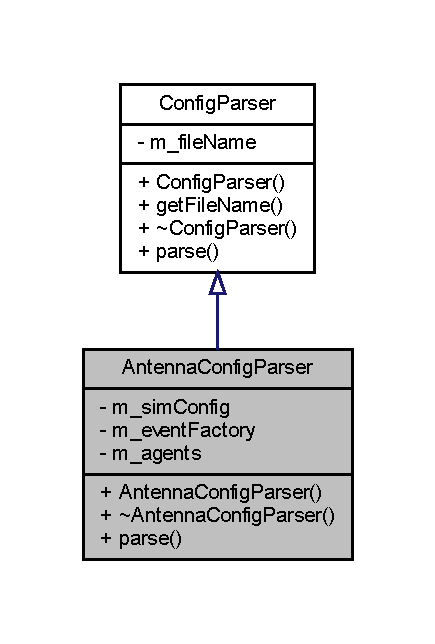
\includegraphics[width=209pt]{class_antenna_config_parser__inherit__graph}
\end{center}
\end{figure}


Collaboration diagram for Antenna\+Config\+Parser\+:
\nopagebreak
\begin{figure}[H]
\begin{center}
\leavevmode
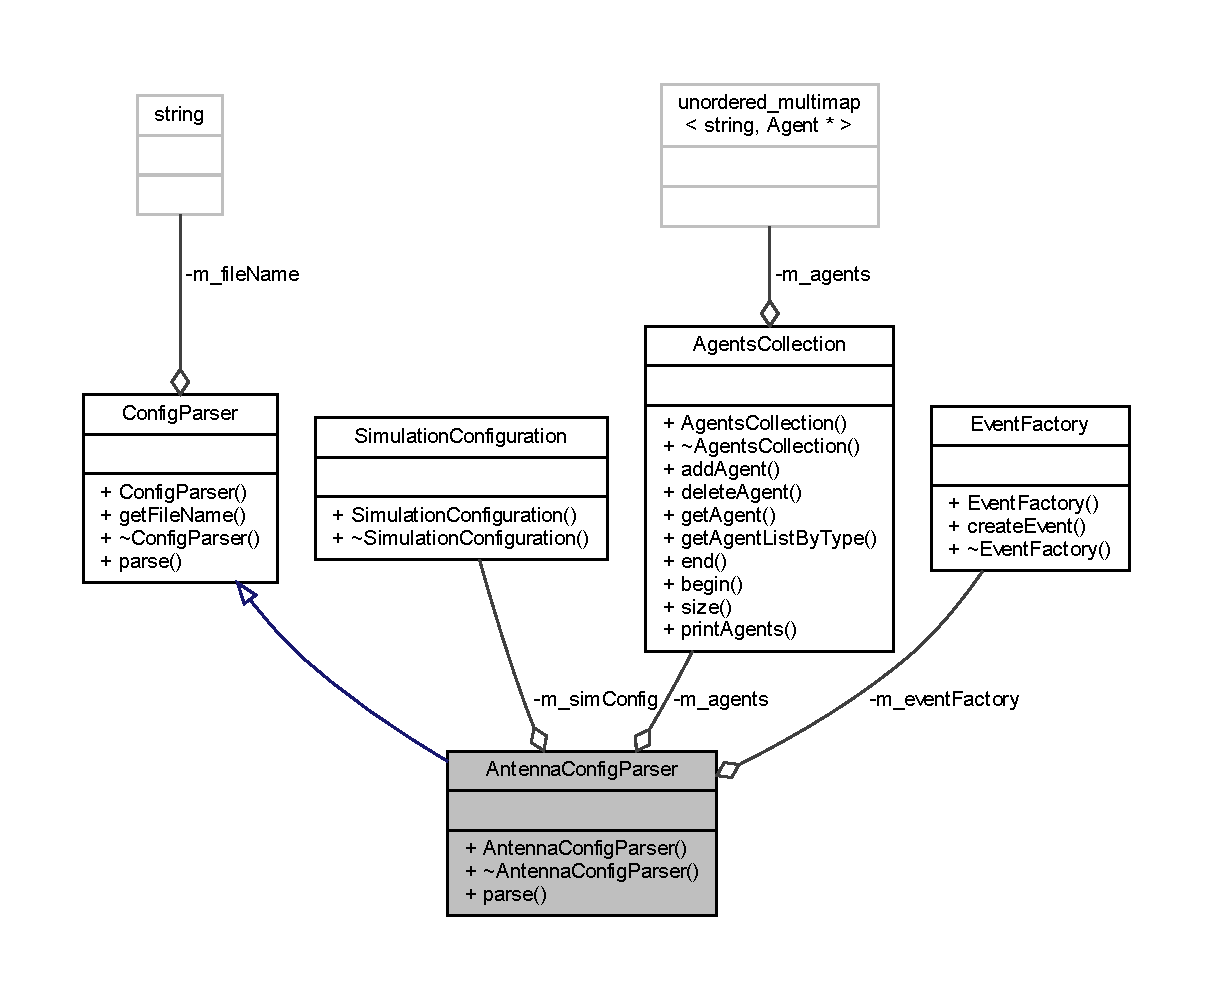
\includegraphics[width=350pt]{class_antenna_config_parser__coll__graph}
\end{center}
\end{figure}
\doxysubsection*{Public Member Functions}
\begin{DoxyCompactItemize}
\item 
\mbox{\hyperlink{class_antenna_config_parser_abaa2fda855a6f540abcac030fd8593f0}{Antenna\+Config\+Parser}} (const string \&file\+Name, \mbox{\hyperlink{class_simulation_configuration}{Simulation\+Configuration}} $\ast$sc, \mbox{\hyperlink{class_agents_collection}{Agents\+Collection}} $\ast$ag, \mbox{\hyperlink{class_event_factory}{Event\+Factory}} $\ast$ev\+Factory)
\item 
virtual \mbox{\hyperlink{class_antenna_config_parser_a8383797b060d1a52c1a255242d5047d2}{$\sim$\+Antenna\+Config\+Parser}} ()
\item 
void \mbox{\hyperlink{class_antenna_config_parser_a19b457a8adbecb36dc97b2449dae76c9}{parse}} () override
\end{DoxyCompactItemize}
\doxysubsection*{Private Attributes}
\begin{DoxyCompactItemize}
\item 
\mbox{\hyperlink{class_simulation_configuration}{Simulation\+Configuration}} $\ast$ \mbox{\hyperlink{class_antenna_config_parser_a1c17aac32514f4962711a531c7fec6be}{m\+\_\+sim\+Config}}
\item 
\mbox{\hyperlink{class_event_factory}{Event\+Factory}} $\ast$ \mbox{\hyperlink{class_antenna_config_parser_af364fc3d782f515761ba1ce630eb51be}{m\+\_\+event\+Factory}}
\item 
\mbox{\hyperlink{class_agents_collection}{Agents\+Collection}} $\ast$ \mbox{\hyperlink{class_antenna_config_parser_a3a2762b82f4d177b4754865e6292cf5b}{m\+\_\+agents}}
\end{DoxyCompactItemize}


\doxysubsection{Detailed Description}
Parses the antenna configuration file specified by \char`\"{}-\/a\char`\"{} option in the command line and builds the antenna objects. This file is named antenna.\+xml in all example configuration folders. While it parses the parameters of each antenna, it builds \mbox{\hyperlink{class_antenna}{Antenna}} objects and adds them to the \mbox{\hyperlink{class_agents_collection}{Agents\+Collection}} container. 

\doxysubsection{Constructor \& Destructor Documentation}
\mbox{\Hypertarget{class_antenna_config_parser_abaa2fda855a6f540abcac030fd8593f0}\label{class_antenna_config_parser_abaa2fda855a6f540abcac030fd8593f0}} 
\index{AntennaConfigParser@{AntennaConfigParser}!AntennaConfigParser@{AntennaConfigParser}}
\index{AntennaConfigParser@{AntennaConfigParser}!AntennaConfigParser@{AntennaConfigParser}}
\doxysubsubsection{\texorpdfstring{AntennaConfigParser()}{AntennaConfigParser()}}
{\footnotesize\ttfamily Antenna\+Config\+Parser\+::\+Antenna\+Config\+Parser (\begin{DoxyParamCaption}\item[{const string \&}]{file\+Name,  }\item[{\mbox{\hyperlink{class_simulation_configuration}{Simulation\+Configuration}} $\ast$}]{sc,  }\item[{\mbox{\hyperlink{class_agents_collection}{Agents\+Collection}} $\ast$}]{ag,  }\item[{\mbox{\hyperlink{class_event_factory}{Event\+Factory}} $\ast$}]{ev\+Factory }\end{DoxyParamCaption})}

Constructor of the class. It takes the filename of the antenna configuration files, a pointer to the \mbox{\hyperlink{class_simulation_configuration}{Simulation\+Configuration}} object, a pointer to the \mbox{\hyperlink{class_agents_collection}{Agents\+Collection}} container class and a pointer to the \mbox{\hyperlink{class_event_factory}{Event\+Factory}}. The \mbox{\hyperlink{class_agents_collection}{Agents\+Collection}} and \mbox{\hyperlink{class_event_factory}{Event\+Factory}} object are created outside, in the caller of this constructor, in this case the constructor of the \mbox{\hyperlink{class_world}{World}} object. The \mbox{\hyperlink{class_simulation_configuration}{Simulation\+Configuration}} object is also created by the constructor of the \mbox{\hyperlink{class_world}{World}} object by parsing the simulation configuration file. While this constructor parses the antenna configuration file, an \mbox{\hyperlink{class_antenna_configuration}{Antenna\+Configuration}} object is created for each antenna. This object encapsulates all required parameters to build an \mbox{\hyperlink{class_antenna}{Antenna}} object and it is passed to the constructor of the \mbox{\hyperlink{class_antenna}{Antenna}} class. 
\begin{DoxyParams}{Parameters}
{\em file\+Name} & the name of the antenna configuration file, given in the command line of the software with \char`\"{}-\/a\char`\"{} option. \\
\hline
{\em sc} & a pointer to the \mbox{\hyperlink{class_simulation_configuration}{Simulation\+Configuration}} object created by the \mbox{\hyperlink{class_simulation_configuration_parser}{Simulation\+Configuration\+Parser}}. It contains the parameters of the simulation read from the simulation configuration file, given in the command line of the software with \char`\"{}-\/s\char`\"{} option. \\
\hline
{\em ag} & a pointer to the \mbox{\hyperlink{class_agents_collection}{Agents\+Collection}} container class created by the constructor of the \mbox{\hyperlink{class_world}{World}} class. \\
\hline
{\em ev\+Factory} & a pointer to the \mbox{\hyperlink{class_event_factory}{Event\+Factory}} class created by the constructor of the \mbox{\hyperlink{class_world}{World}} class. This factory is used by each \mbox{\hyperlink{class_antenna}{Antenna}} object the generate network events. \\
\hline
\end{DoxyParams}
\mbox{\Hypertarget{class_antenna_config_parser_a8383797b060d1a52c1a255242d5047d2}\label{class_antenna_config_parser_a8383797b060d1a52c1a255242d5047d2}} 
\index{AntennaConfigParser@{AntennaConfigParser}!````~AntennaConfigParser@{$\sim$AntennaConfigParser}}
\index{````~AntennaConfigParser@{$\sim$AntennaConfigParser}!AntennaConfigParser@{AntennaConfigParser}}
\doxysubsubsection{\texorpdfstring{$\sim$AntennaConfigParser()}{~AntennaConfigParser()}}
{\footnotesize\ttfamily virtual Antenna\+Config\+Parser\+::$\sim$\+Antenna\+Config\+Parser (\begin{DoxyParamCaption}{ }\end{DoxyParamCaption})\hspace{0.3cm}{\ttfamily [virtual]}}

Default destructor. 

\doxysubsection{Member Function Documentation}
\mbox{\Hypertarget{class_antenna_config_parser_a19b457a8adbecb36dc97b2449dae76c9}\label{class_antenna_config_parser_a19b457a8adbecb36dc97b2449dae76c9}} 
\index{AntennaConfigParser@{AntennaConfigParser}!parse@{parse}}
\index{parse@{parse}!AntennaConfigParser@{AntennaConfigParser}}
\doxysubsubsection{\texorpdfstring{parse()}{parse()}}
{\footnotesize\ttfamily void Antenna\+Config\+Parser\+::parse (\begin{DoxyParamCaption}{ }\end{DoxyParamCaption})\hspace{0.3cm}{\ttfamily [override]}, {\ttfamily [virtual]}}

A method to parse the antenna configuration file. While it parses this file, it builds an \mbox{\hyperlink{class_antenna_configuration}{Antenna\+Configuration}} object for each antenna and passes it to the constructor of the \mbox{\hyperlink{class_antenna}{Antenna}} class. All \mbox{\hyperlink{class_antenna}{Antenna}} objects are added to the \mbox{\hyperlink{class_agents_collection}{Agents\+Collection}} container class. 

Implements \mbox{\hyperlink{class_config_parser_afc13df32c129e923c7aa33db7413dd2e}{Config\+Parser}}.



\doxysubsection{Member Data Documentation}
\mbox{\Hypertarget{class_antenna_config_parser_a3a2762b82f4d177b4754865e6292cf5b}\label{class_antenna_config_parser_a3a2762b82f4d177b4754865e6292cf5b}} 
\index{AntennaConfigParser@{AntennaConfigParser}!m\_agents@{m\_agents}}
\index{m\_agents@{m\_agents}!AntennaConfigParser@{AntennaConfigParser}}
\doxysubsubsection{\texorpdfstring{m\_agents}{m\_agents}}
{\footnotesize\ttfamily \mbox{\hyperlink{class_agents_collection}{Agents\+Collection}}$\ast$ Antenna\+Config\+Parser\+::m\+\_\+agents\hspace{0.3cm}{\ttfamily [private]}}

\mbox{\Hypertarget{class_antenna_config_parser_af364fc3d782f515761ba1ce630eb51be}\label{class_antenna_config_parser_af364fc3d782f515761ba1ce630eb51be}} 
\index{AntennaConfigParser@{AntennaConfigParser}!m\_eventFactory@{m\_eventFactory}}
\index{m\_eventFactory@{m\_eventFactory}!AntennaConfigParser@{AntennaConfigParser}}
\doxysubsubsection{\texorpdfstring{m\_eventFactory}{m\_eventFactory}}
{\footnotesize\ttfamily \mbox{\hyperlink{class_event_factory}{Event\+Factory}}$\ast$ Antenna\+Config\+Parser\+::m\+\_\+event\+Factory\hspace{0.3cm}{\ttfamily [private]}}

\mbox{\Hypertarget{class_antenna_config_parser_a1c17aac32514f4962711a531c7fec6be}\label{class_antenna_config_parser_a1c17aac32514f4962711a531c7fec6be}} 
\index{AntennaConfigParser@{AntennaConfigParser}!m\_simConfig@{m\_simConfig}}
\index{m\_simConfig@{m\_simConfig}!AntennaConfigParser@{AntennaConfigParser}}
\doxysubsubsection{\texorpdfstring{m\_simConfig}{m\_simConfig}}
{\footnotesize\ttfamily \mbox{\hyperlink{class_simulation_configuration}{Simulation\+Configuration}}$\ast$ Antenna\+Config\+Parser\+::m\+\_\+sim\+Config\hspace{0.3cm}{\ttfamily [private]}}



The documentation for this class was generated from the following file\+:\begin{DoxyCompactItemize}
\item 
include/parsers/\mbox{\hyperlink{_antenna_config_parser_8h}{Antenna\+Config\+Parser.\+h}}\end{DoxyCompactItemize}

\hypertarget{class_antenna_configuration}{}\doxysection{Antenna\+Configuration Class Reference}
\label{class_antenna_configuration}\index{AntennaConfiguration@{AntennaConfiguration}}


{\ttfamily \#include $<$Antenna\+Configuration.\+h$>$}



Collaboration diagram for Antenna\+Configuration\+:
\nopagebreak
\begin{figure}[H]
\begin{center}
\leavevmode
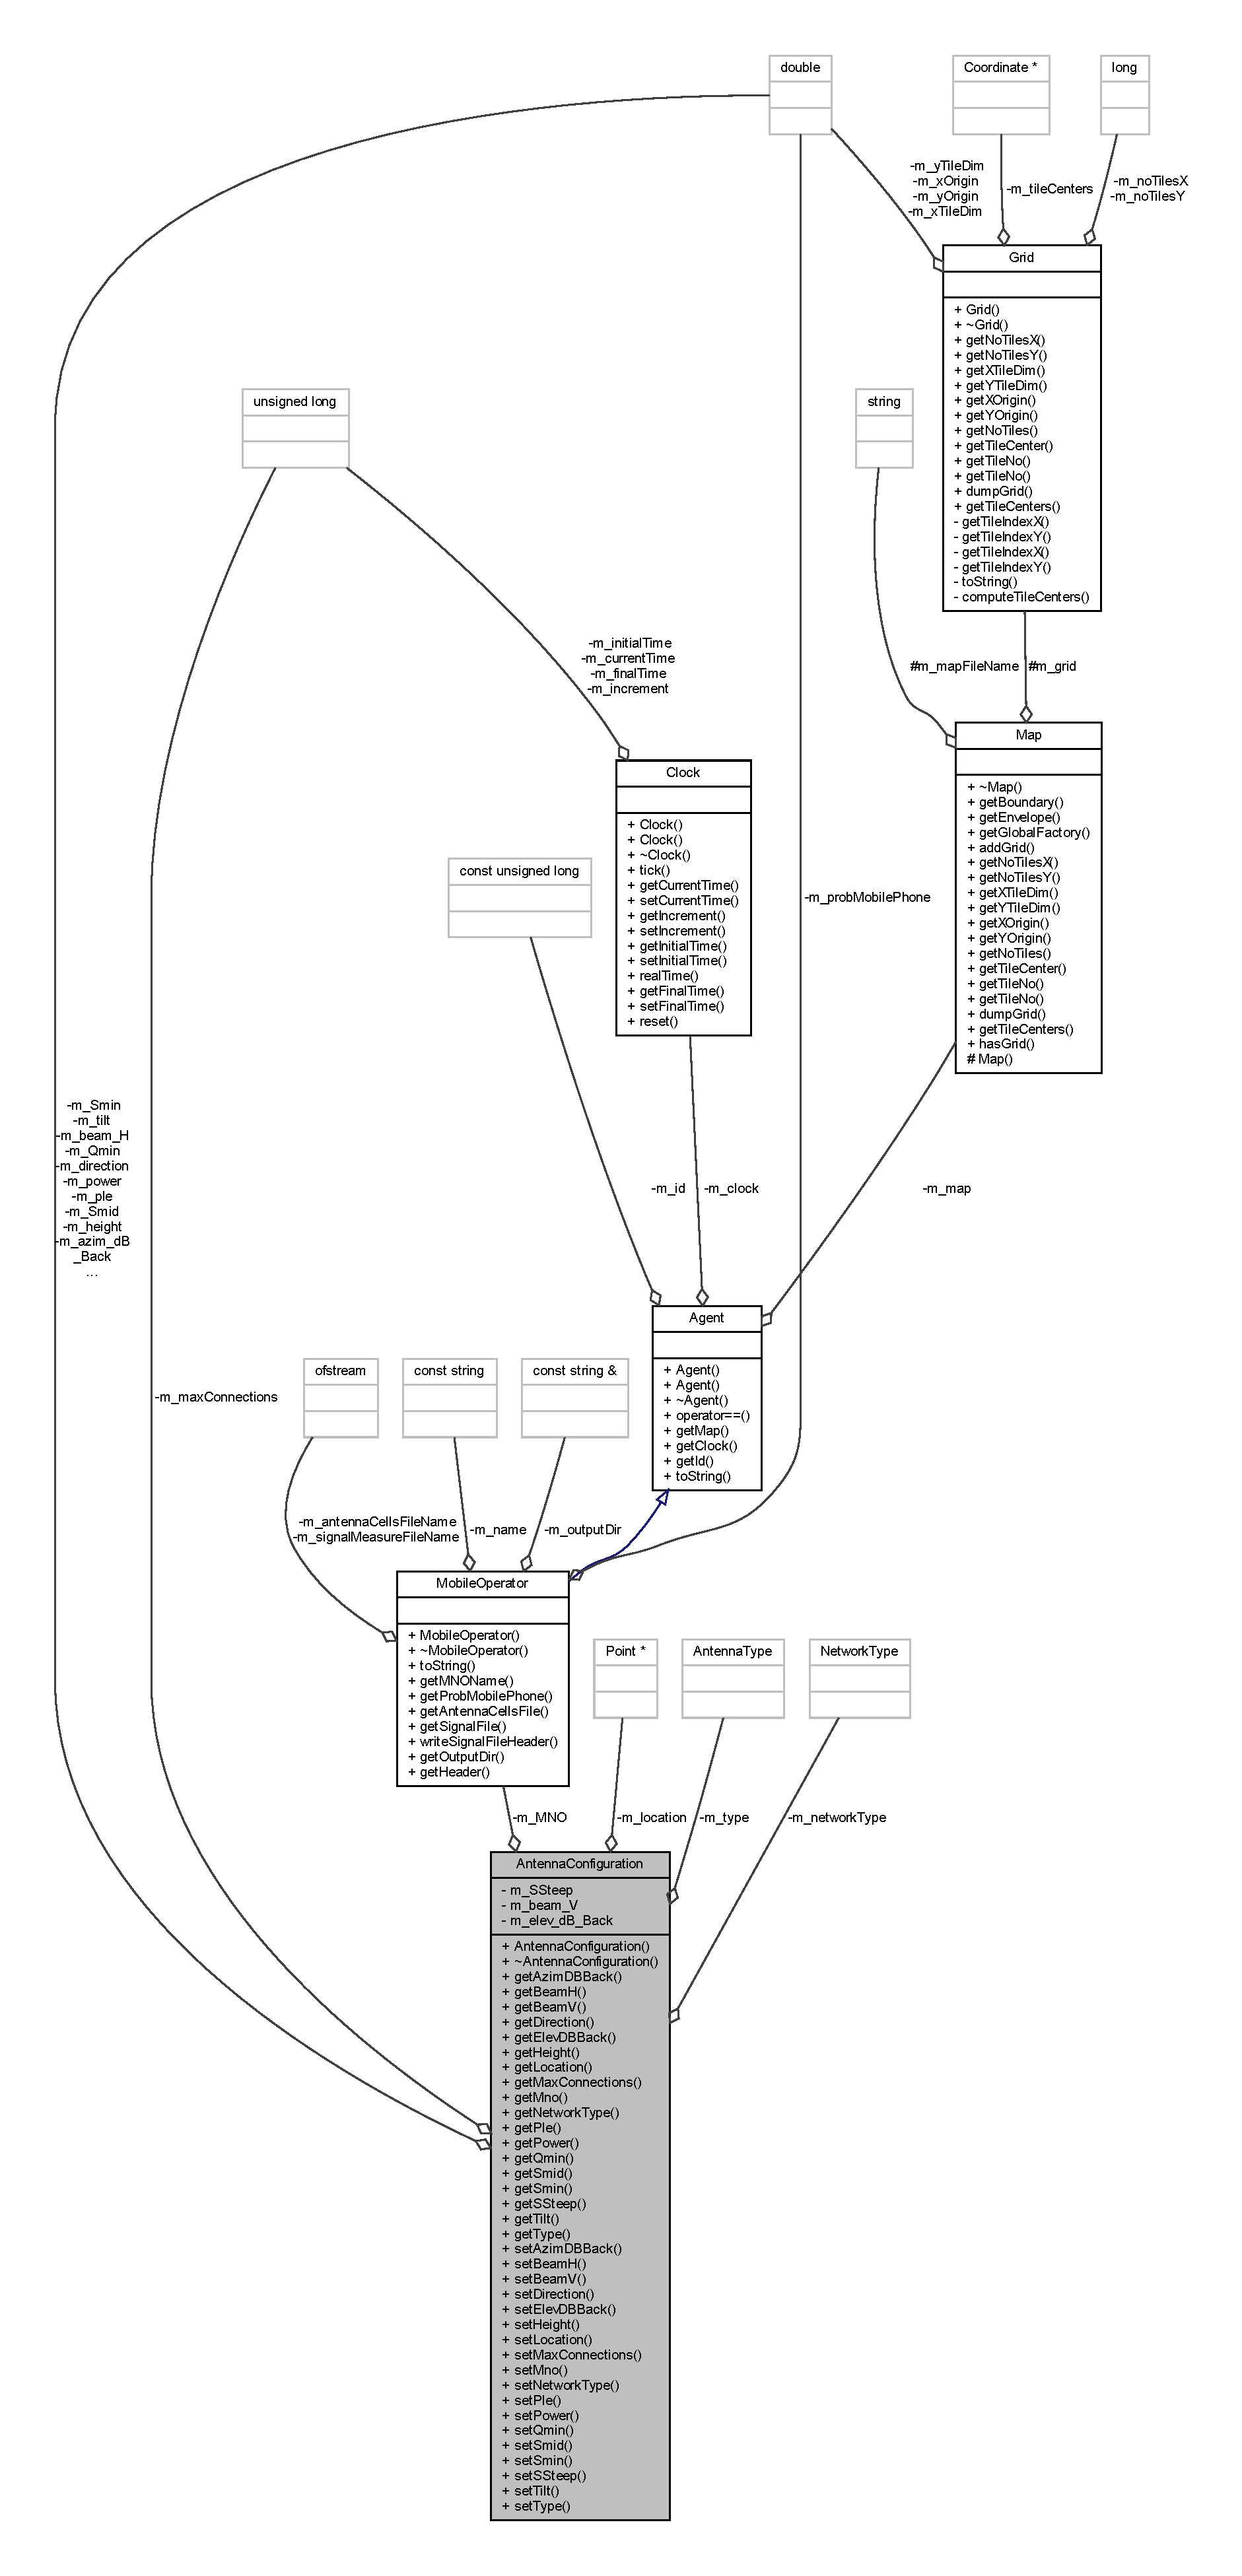
\includegraphics[height=550pt]{class_antenna_configuration__coll__graph}
\end{center}
\end{figure}
\doxysubsection*{Public Member Functions}
\begin{DoxyCompactItemize}
\item 
\mbox{\hyperlink{class_antenna_configuration_a11725cd788f01f94b5219b982ff6ada2}{Antenna\+Configuration}} ()
\item 
virtual \mbox{\hyperlink{class_antenna_configuration_a4b7e714dd62bb4c94ed29e872fca8d72}{$\sim$\+Antenna\+Configuration}} ()
\item 
double \mbox{\hyperlink{class_antenna_configuration_a5cddafc9a971b453d92489693a551650}{get\+Azim\+D\+B\+Back}} () const
\item 
double \mbox{\hyperlink{class_antenna_configuration_a0b1c9e7cc1d17fe9fb5f1ba472088f23}{get\+BeamH}} () const
\item 
double \mbox{\hyperlink{class_antenna_configuration_a6406e1b5777196a8660e8e704218e14e}{get\+BeamV}} () const
\item 
double \mbox{\hyperlink{class_antenna_configuration_ac827bf19cb01bc6a9599aa05c9041dfe}{get\+Direction}} () const
\item 
double \mbox{\hyperlink{class_antenna_configuration_a8305a9902f99d774e36d8719fc1f6873}{get\+Elev\+D\+B\+Back}} () const
\item 
double \mbox{\hyperlink{class_antenna_configuration_af35be2fa94fceab1ef7e7066195169a1}{get\+Height}} () const
\item 
Point $\ast$ \mbox{\hyperlink{class_antenna_configuration_a8ebe3060572c12f9fa7809e2128a712c}{get\+Location}} () const
\item 
unsigned long \mbox{\hyperlink{class_antenna_configuration_a451a2ff81812914d55fabea2709723a7}{get\+Max\+Connections}} () const
\item 
\mbox{\hyperlink{class_mobile_operator}{Mobile\+Operator}} $\ast$ \mbox{\hyperlink{class_antenna_configuration_a7c539badb16c9a703ceaf5b0a883c3b2}{get\+Mno}} () const
\item 
\mbox{\hyperlink{_network_type_8h_a3a159600500d5d7248be5bd1ca1f8d83}{Network\+Type}} \mbox{\hyperlink{class_antenna_configuration_a6b18bc08eca40da574ebe92463dd66e2}{get\+Network\+Type}} () const
\item 
double \mbox{\hyperlink{class_antenna_configuration_ad304fc94112a1ae77444ad809374eefa}{get\+Ple}} () const
\item 
double \mbox{\hyperlink{class_antenna_configuration_a76d2e0633d21f3584bdd5025082d0467}{get\+Power}} () const
\item 
double \mbox{\hyperlink{class_antenna_configuration_aa8ef41020e71f4ffc0c5ef206f02e681}{get\+Qmin}} () const
\item 
double \mbox{\hyperlink{class_antenna_configuration_a033716bd6fdaea822901d97efc1556ac}{get\+Smid}} () const
\item 
double \mbox{\hyperlink{class_antenna_configuration_a60cae03c199b615cc42e16ad6bdedd56}{get\+Smin}} () const
\item 
double \mbox{\hyperlink{class_antenna_configuration_ad6e8e95dc76bc0221ad44ab1289e346b}{get\+S\+Steep}} () const
\item 
double \mbox{\hyperlink{class_antenna_configuration_a95d4b3c83fe0db056066c349600e8aed}{get\+Tilt}} () const
\item 
\mbox{\hyperlink{_antenna_type_8h_a7b678b5cb9dedc607131200119d96b16}{Antenna\+Type}} \mbox{\hyperlink{class_antenna_configuration_a83a19d2008a42d81f514c4a5d1ab2b99}{get\+Type}} () const
\item 
void \mbox{\hyperlink{class_antenna_configuration_a19e4717651af21acc219a346fcd88a91}{set\+Azim\+D\+B\+Back}} (double azim\+D\+B\+Back)
\item 
void \mbox{\hyperlink{class_antenna_configuration_ae93a4c9e64b7ba3e2623d44f812c297c}{set\+BeamH}} (double beamH)
\item 
void \mbox{\hyperlink{class_antenna_configuration_aeb6d74d13ebe0210ae475dd0bbf5252e}{set\+BeamV}} (double beamV)
\item 
void \mbox{\hyperlink{class_antenna_configuration_a85eb2e0469eff599892f787ec5bc5566}{set\+Direction}} (double direction)
\item 
void \mbox{\hyperlink{class_antenna_configuration_a585bb2d4395cf9847b3d9885516c22ad}{set\+Elev\+D\+B\+Back}} (double elev\+D\+B\+Back)
\item 
void \mbox{\hyperlink{class_antenna_configuration_ac1f645965b5257a9768affe271f6580a}{set\+Height}} (double height)
\item 
void \mbox{\hyperlink{class_antenna_configuration_ab1e405e0fef94d4492cd70d9632e36e7}{set\+Location}} (Point $\ast$location)
\item 
void \mbox{\hyperlink{class_antenna_configuration_a1028e3ddfd2a0fe74c8175954cd12046}{set\+Max\+Connections}} (unsigned long max\+Connections)
\item 
void \mbox{\hyperlink{class_antenna_configuration_a6e20ae143ffddbc36340b2230627df6d}{set\+Mno}} (\mbox{\hyperlink{class_mobile_operator}{Mobile\+Operator}} $\ast$mno)
\item 
void \mbox{\hyperlink{class_antenna_configuration_ad8c11f302d4ab2de6faf5dd3435390cd}{set\+Network\+Type}} (\mbox{\hyperlink{_network_type_8h_a3a159600500d5d7248be5bd1ca1f8d83}{Network\+Type}} network\+Type)
\item 
void \mbox{\hyperlink{class_antenna_configuration_af15d4914891fbb0325132496e6818444}{set\+Ple}} (double ple)
\item 
void \mbox{\hyperlink{class_antenna_configuration_a16c17c53bf76363559ab01c620a52d24}{set\+Power}} (double power)
\item 
void \mbox{\hyperlink{class_antenna_configuration_a16919abe381a082abf7a6841aeb0f700}{set\+Qmin}} (double qmin)
\item 
void \mbox{\hyperlink{class_antenna_configuration_a89a5071e0521dcbaf972ffe017df3f91}{set\+Smid}} (double Smid)
\item 
void \mbox{\hyperlink{class_antenna_configuration_ad06bb9b4ee430250c506c70dfd95f4ea}{set\+Smin}} (double Smin)
\item 
void \mbox{\hyperlink{class_antenna_configuration_a6d85a7b51cd1bc1df0fd8b5eef353b4f}{set\+S\+Steep}} (double S\+Steep)
\item 
void \mbox{\hyperlink{class_antenna_configuration_ac37b907c7c798a0db1a65b8b2281b0d6}{set\+Tilt}} (double tilt)
\item 
void \mbox{\hyperlink{class_antenna_configuration_aa7d57c553024b6e62862075ee141eba9}{set\+Type}} (\mbox{\hyperlink{_antenna_type_8h_a7b678b5cb9dedc607131200119d96b16}{Antenna\+Type}} type)
\end{DoxyCompactItemize}
\doxysubsection*{Private Attributes}
\begin{DoxyCompactItemize}
\item 
double \mbox{\hyperlink{class_antenna_configuration_a3808b677bdcb29316250d1b087b0867d}{m\+\_\+ple}}
\item 
double \mbox{\hyperlink{class_antenna_configuration_a43aedcbf8ff7911b060af6a7502fbec3}{m\+\_\+power}}
\item 
unsigned long \mbox{\hyperlink{class_antenna_configuration_ac66231329d56b8e9a62344b84e14ffed}{m\+\_\+max\+Connections}}
\item 
double \mbox{\hyperlink{class_antenna_configuration_ac53a084ade49b15bd08edad443550728}{m\+\_\+\+Smid}}
\item 
double \mbox{\hyperlink{class_antenna_configuration_ae565a9d615d0551f6aabbbece39699c0}{m\+\_\+\+S\+Steep}}
\item 
\mbox{\hyperlink{_antenna_type_8h_a7b678b5cb9dedc607131200119d96b16}{Antenna\+Type}} \mbox{\hyperlink{class_antenna_configuration_a41fbcffdbf246e235ec9ce4e86de3c5d}{m\+\_\+type}}
\item 
double \mbox{\hyperlink{class_antenna_configuration_a4936a01295b1cabfc52df32ce31ed5b2}{m\+\_\+height}}
\item 
double \mbox{\hyperlink{class_antenna_configuration_a01a316a5bedae09e787d0de6a8fc31b0}{m\+\_\+tilt}}
\item 
double \mbox{\hyperlink{class_antenna_configuration_a02cf839b205b99b5b48408c6116ede07}{m\+\_\+beam\+\_\+V}}
\item 
double \mbox{\hyperlink{class_antenna_configuration_aba46332a8290cd61cc334f9e9bd7e08d}{m\+\_\+beam\+\_\+H}}
\item 
double \mbox{\hyperlink{class_antenna_configuration_a37087cd72d01edec5c5b683d11ee6008}{m\+\_\+azim\+\_\+d\+B\+\_\+\+Back}}
\item 
double \mbox{\hyperlink{class_antenna_configuration_a1e95c09afeb7d9714697b5ff73269fcf}{m\+\_\+elev\+\_\+d\+B\+\_\+\+Back}}
\item 
double \mbox{\hyperlink{class_antenna_configuration_a62b26935a5b14a6d3aef85e400834dd6}{m\+\_\+direction}}
\item 
double \mbox{\hyperlink{class_antenna_configuration_ab483fc115fa1b3bbe1bf9c43cd520e18}{m\+\_\+\+Smin}}
\item 
double \mbox{\hyperlink{class_antenna_configuration_a34abf6a84e270ecacf7fe1e4655f2dfa}{m\+\_\+\+Qmin}}
\item 
\mbox{\hyperlink{_network_type_8h_a3a159600500d5d7248be5bd1ca1f8d83}{Network\+Type}} \mbox{\hyperlink{class_antenna_configuration_ae41f480fa0cd6588a9b6c46770e7a880}{m\+\_\+network\+Type}}
\item 
Point $\ast$ \mbox{\hyperlink{class_antenna_configuration_a623c485b88938677890d08e67175331c}{m\+\_\+location}}
\item 
\mbox{\hyperlink{class_mobile_operator}{Mobile\+Operator}} $\ast$ \mbox{\hyperlink{class_antenna_configuration_a0e850470e8e2a56c9d95fd80bdac54f4}{m\+\_\+\+M\+NO}}
\end{DoxyCompactItemize}


\doxysubsection{Detailed Description}
A class that contains all the technical parameters needed to build an \mbox{\hyperlink{class_antenna}{Antenna}} object. This object is build during the parsing of the antenna configuration file and it is passed to the constructor of the \mbox{\hyperlink{class_antenna}{Antenna}} object. 

\doxysubsection{Constructor \& Destructor Documentation}
\mbox{\Hypertarget{class_antenna_configuration_a11725cd788f01f94b5219b982ff6ada2}\label{class_antenna_configuration_a11725cd788f01f94b5219b982ff6ada2}} 
\index{AntennaConfiguration@{AntennaConfiguration}!AntennaConfiguration@{AntennaConfiguration}}
\index{AntennaConfiguration@{AntennaConfiguration}!AntennaConfiguration@{AntennaConfiguration}}
\doxysubsubsection{\texorpdfstring{AntennaConfiguration()}{AntennaConfiguration()}}
{\footnotesize\ttfamily Antenna\+Configuration\+::\+Antenna\+Configuration (\begin{DoxyParamCaption}{ }\end{DoxyParamCaption})}

The constructor of the class. It initializes all members of the class with the default values specified in the \mbox{\hyperlink{class_constants}{Constants}} class. While the configuration file is parsed, the setter methods are used to set the values of the corresponding parameter. \mbox{\Hypertarget{class_antenna_configuration_a4b7e714dd62bb4c94ed29e872fca8d72}\label{class_antenna_configuration_a4b7e714dd62bb4c94ed29e872fca8d72}} 
\index{AntennaConfiguration@{AntennaConfiguration}!````~AntennaConfiguration@{$\sim$AntennaConfiguration}}
\index{````~AntennaConfiguration@{$\sim$AntennaConfiguration}!AntennaConfiguration@{AntennaConfiguration}}
\doxysubsubsection{\texorpdfstring{$\sim$AntennaConfiguration()}{~AntennaConfiguration()}}
{\footnotesize\ttfamily virtual Antenna\+Configuration\+::$\sim$\+Antenna\+Configuration (\begin{DoxyParamCaption}{ }\end{DoxyParamCaption})\hspace{0.3cm}{\ttfamily [virtual]}}

The default destructor of the class. 

\doxysubsection{Member Function Documentation}
\mbox{\Hypertarget{class_antenna_configuration_a5cddafc9a971b453d92489693a551650}\label{class_antenna_configuration_a5cddafc9a971b453d92489693a551650}} 
\index{AntennaConfiguration@{AntennaConfiguration}!getAzimDBBack@{getAzimDBBack}}
\index{getAzimDBBack@{getAzimDBBack}!AntennaConfiguration@{AntennaConfiguration}}
\doxysubsubsection{\texorpdfstring{getAzimDBBack()}{getAzimDBBack()}}
{\footnotesize\ttfamily double Antenna\+Configuration\+::get\+Azim\+D\+B\+Back (\begin{DoxyParamCaption}{ }\end{DoxyParamCaption}) const}

Returns the difference in signal strength between front and back in the azimuth plane for directional antennas. \begin{DoxyReturn}{Returns}
the difference in signal strength between front and back in the azimuth plane for directional antennas. 
\end{DoxyReturn}
\mbox{\Hypertarget{class_antenna_configuration_a0b1c9e7cc1d17fe9fb5f1ba472088f23}\label{class_antenna_configuration_a0b1c9e7cc1d17fe9fb5f1ba472088f23}} 
\index{AntennaConfiguration@{AntennaConfiguration}!getBeamH@{getBeamH}}
\index{getBeamH@{getBeamH}!AntennaConfiguration@{AntennaConfiguration}}
\doxysubsubsection{\texorpdfstring{getBeamH()}{getBeamH()}}
{\footnotesize\ttfamily double Antenna\+Configuration\+::get\+BeamH (\begin{DoxyParamCaption}{ }\end{DoxyParamCaption}) const}

Returns the horizontal beam width for directional antennas. \begin{DoxyReturn}{Returns}
the horizontal beam width for directional antennas. 
\end{DoxyReturn}
\mbox{\Hypertarget{class_antenna_configuration_a6406e1b5777196a8660e8e704218e14e}\label{class_antenna_configuration_a6406e1b5777196a8660e8e704218e14e}} 
\index{AntennaConfiguration@{AntennaConfiguration}!getBeamV@{getBeamV}}
\index{getBeamV@{getBeamV}!AntennaConfiguration@{AntennaConfiguration}}
\doxysubsubsection{\texorpdfstring{getBeamV()}{getBeamV()}}
{\footnotesize\ttfamily double Antenna\+Configuration\+::get\+BeamV (\begin{DoxyParamCaption}{ }\end{DoxyParamCaption}) const}

Returns the vertical beam width for directional antennas. \begin{DoxyReturn}{Returns}
the vertical beam width for directional antennas. 
\end{DoxyReturn}
\mbox{\Hypertarget{class_antenna_configuration_ac827bf19cb01bc6a9599aa05c9041dfe}\label{class_antenna_configuration_ac827bf19cb01bc6a9599aa05c9041dfe}} 
\index{AntennaConfiguration@{AntennaConfiguration}!getDirection@{getDirection}}
\index{getDirection@{getDirection}!AntennaConfiguration@{AntennaConfiguration}}
\doxysubsubsection{\texorpdfstring{getDirection()}{getDirection()}}
{\footnotesize\ttfamily double Antenna\+Configuration\+::get\+Direction (\begin{DoxyParamCaption}{ }\end{DoxyParamCaption}) const}

Returns the direction angle for directional antennas. \begin{DoxyReturn}{Returns}
the direction angle for directional antennas. 
\end{DoxyReturn}
\mbox{\Hypertarget{class_antenna_configuration_a8305a9902f99d774e36d8719fc1f6873}\label{class_antenna_configuration_a8305a9902f99d774e36d8719fc1f6873}} 
\index{AntennaConfiguration@{AntennaConfiguration}!getElevDBBack@{getElevDBBack}}
\index{getElevDBBack@{getElevDBBack}!AntennaConfiguration@{AntennaConfiguration}}
\doxysubsubsection{\texorpdfstring{getElevDBBack()}{getElevDBBack()}}
{\footnotesize\ttfamily double Antenna\+Configuration\+::get\+Elev\+D\+B\+Back (\begin{DoxyParamCaption}{ }\end{DoxyParamCaption}) const}


\begin{DoxyItemize}
\item Returns the difference in signal strength between front and back in the elevation plane for directional antennas. \begin{DoxyReturn}{Returns}
the difference in signal strength between front and back in the elevation plane for directional antennas. 
\end{DoxyReturn}

\end{DoxyItemize}\mbox{\Hypertarget{class_antenna_configuration_af35be2fa94fceab1ef7e7066195169a1}\label{class_antenna_configuration_af35be2fa94fceab1ef7e7066195169a1}} 
\index{AntennaConfiguration@{AntennaConfiguration}!getHeight@{getHeight}}
\index{getHeight@{getHeight}!AntennaConfiguration@{AntennaConfiguration}}
\doxysubsubsection{\texorpdfstring{getHeight()}{getHeight()}}
{\footnotesize\ttfamily double Antenna\+Configuration\+::get\+Height (\begin{DoxyParamCaption}{ }\end{DoxyParamCaption}) const}

Returns the height of the antenna (the z coordinate of location of the antenna). \begin{DoxyReturn}{Returns}
the height of the antenna (the z coordinate of location of the antenna). 
\end{DoxyReturn}
\mbox{\Hypertarget{class_antenna_configuration_a8ebe3060572c12f9fa7809e2128a712c}\label{class_antenna_configuration_a8ebe3060572c12f9fa7809e2128a712c}} 
\index{AntennaConfiguration@{AntennaConfiguration}!getLocation@{getLocation}}
\index{getLocation@{getLocation}!AntennaConfiguration@{AntennaConfiguration}}
\doxysubsubsection{\texorpdfstring{getLocation()}{getLocation()}}
{\footnotesize\ttfamily Point$\ast$ Antenna\+Configuration\+::get\+Location (\begin{DoxyParamCaption}{ }\end{DoxyParamCaption}) const}

Returns the location of the antenna on the map. \begin{DoxyReturn}{Returns}
the location of the antenna on the map. 
\end{DoxyReturn}
\mbox{\Hypertarget{class_antenna_configuration_a451a2ff81812914d55fabea2709723a7}\label{class_antenna_configuration_a451a2ff81812914d55fabea2709723a7}} 
\index{AntennaConfiguration@{AntennaConfiguration}!getMaxConnections@{getMaxConnections}}
\index{getMaxConnections@{getMaxConnections}!AntennaConfiguration@{AntennaConfiguration}}
\doxysubsubsection{\texorpdfstring{getMaxConnections()}{getMaxConnections()}}
{\footnotesize\ttfamily unsigned long Antenna\+Configuration\+::get\+Max\+Connections (\begin{DoxyParamCaption}{ }\end{DoxyParamCaption}) const}

Returns the maximum number of simultaneous connections an antenna can accept. \begin{DoxyReturn}{Returns}
the maximum number of simultaneous connections an antenna can accept. 
\end{DoxyReturn}
\mbox{\Hypertarget{class_antenna_configuration_a7c539badb16c9a703ceaf5b0a883c3b2}\label{class_antenna_configuration_a7c539badb16c9a703ceaf5b0a883c3b2}} 
\index{AntennaConfiguration@{AntennaConfiguration}!getMno@{getMno}}
\index{getMno@{getMno}!AntennaConfiguration@{AntennaConfiguration}}
\doxysubsubsection{\texorpdfstring{getMno()}{getMno()}}
{\footnotesize\ttfamily \mbox{\hyperlink{class_mobile_operator}{Mobile\+Operator}}$\ast$ Antenna\+Configuration\+::get\+Mno (\begin{DoxyParamCaption}{ }\end{DoxyParamCaption}) const}

Returns a pointer to the \mbox{\hyperlink{class_mobile_operator}{Mobile\+Operator}} object that owns this antenna. \begin{DoxyReturn}{Returns}
a pointer to the \mbox{\hyperlink{class_mobile_operator}{Mobile\+Operator}} object that owns this antenna. 
\end{DoxyReturn}
\mbox{\Hypertarget{class_antenna_configuration_a6b18bc08eca40da574ebe92463dd66e2}\label{class_antenna_configuration_a6b18bc08eca40da574ebe92463dd66e2}} 
\index{AntennaConfiguration@{AntennaConfiguration}!getNetworkType@{getNetworkType}}
\index{getNetworkType@{getNetworkType}!AntennaConfiguration@{AntennaConfiguration}}
\doxysubsubsection{\texorpdfstring{getNetworkType()}{getNetworkType()}}
{\footnotesize\ttfamily \mbox{\hyperlink{_network_type_8h_a3a159600500d5d7248be5bd1ca1f8d83}{Network\+Type}} Antenna\+Configuration\+::get\+Network\+Type (\begin{DoxyParamCaption}{ }\end{DoxyParamCaption}) const}

Returns the network type of the antenna \+: \mbox{\hyperlink{_network_type_8h_a3a159600500d5d7248be5bd1ca1f8d83ac88ee8f01394dbabf5c4487986d04971}{Network\+Type\+::\+\_\+3G}} or \mbox{\hyperlink{_network_type_8h_a3a159600500d5d7248be5bd1ca1f8d83ae5ee9782bb207b843ba97eaa2d0fe26b}{Network\+Type\+::\+\_\+4G}} \begin{DoxyReturn}{Returns}
the network type of the antenna \+: \mbox{\hyperlink{_network_type_8h_a3a159600500d5d7248be5bd1ca1f8d83ac88ee8f01394dbabf5c4487986d04971}{Network\+Type\+::\+\_\+3G}} or \mbox{\hyperlink{_network_type_8h_a3a159600500d5d7248be5bd1ca1f8d83ae5ee9782bb207b843ba97eaa2d0fe26b}{Network\+Type\+::\+\_\+4G}} 
\end{DoxyReturn}
\mbox{\Hypertarget{class_antenna_configuration_ad304fc94112a1ae77444ad809374eefa}\label{class_antenna_configuration_ad304fc94112a1ae77444ad809374eefa}} 
\index{AntennaConfiguration@{AntennaConfiguration}!getPle@{getPle}}
\index{getPle@{getPle}!AntennaConfiguration@{AntennaConfiguration}}
\doxysubsubsection{\texorpdfstring{getPle()}{getPle()}}
{\footnotesize\ttfamily double Antenna\+Configuration\+::get\+Ple (\begin{DoxyParamCaption}{ }\end{DoxyParamCaption}) const}

Returns the path loss exponent (the attenuation factor of the signal). This is a feature of the surrounding environment of the antenna. \begin{DoxyReturn}{Returns}
the path loss exponent (the attenuation factor of the signal). This is a feature of the surrounding environment of the antenna. 
\end{DoxyReturn}
\mbox{\Hypertarget{class_antenna_configuration_a76d2e0633d21f3584bdd5025082d0467}\label{class_antenna_configuration_a76d2e0633d21f3584bdd5025082d0467}} 
\index{AntennaConfiguration@{AntennaConfiguration}!getPower@{getPower}}
\index{getPower@{getPower}!AntennaConfiguration@{AntennaConfiguration}}
\doxysubsubsection{\texorpdfstring{getPower()}{getPower()}}
{\footnotesize\ttfamily double Antenna\+Configuration\+::get\+Power (\begin{DoxyParamCaption}{ }\end{DoxyParamCaption}) const}

Returns the power of the antenna measured in Watts. \begin{DoxyReturn}{Returns}
the power of the antenna in measured Watts. 
\end{DoxyReturn}
\mbox{\Hypertarget{class_antenna_configuration_aa8ef41020e71f4ffc0c5ef206f02e681}\label{class_antenna_configuration_aa8ef41020e71f4ffc0c5ef206f02e681}} 
\index{AntennaConfiguration@{AntennaConfiguration}!getQmin@{getQmin}}
\index{getQmin@{getQmin}!AntennaConfiguration@{AntennaConfiguration}}
\doxysubsubsection{\texorpdfstring{getQmin()}{getQmin()}}
{\footnotesize\ttfamily double Antenna\+Configuration\+::get\+Qmin (\begin{DoxyParamCaption}{ }\end{DoxyParamCaption}) const}

Returns the minimum value of the signal dominance that can be used to connect a mobile device. \begin{DoxyReturn}{Returns}
the minimum value of the signal dominance that can be used to connect a mobile device. 
\end{DoxyReturn}
\mbox{\Hypertarget{class_antenna_configuration_a033716bd6fdaea822901d97efc1556ac}\label{class_antenna_configuration_a033716bd6fdaea822901d97efc1556ac}} 
\index{AntennaConfiguration@{AntennaConfiguration}!getSmid@{getSmid}}
\index{getSmid@{getSmid}!AntennaConfiguration@{AntennaConfiguration}}
\doxysubsubsection{\texorpdfstring{getSmid()}{getSmid()}}
{\footnotesize\ttfamily double Antenna\+Configuration\+::get\+Smid (\begin{DoxyParamCaption}{ }\end{DoxyParamCaption}) const}

Returns the Smid parameter of the signal propagation model. For details see

Salgado, D., Sanguiao, L., Oancea, B. et al. An end-\/to-\/end statistical process with mobile network data for official statistics. E\+PJ Data Science, 10, 20 (2021). \href{https://doi.org/10.1140/epjds/s13688-021-00275-w}{\texttt{ https\+://doi.\+org/10.\+1140/epjds/s13688-\/021-\/00275-\/w}}. \begin{DoxyReturn}{Returns}
the Smid parameter of the signal propagation model. 
\end{DoxyReturn}
\mbox{\Hypertarget{class_antenna_configuration_a60cae03c199b615cc42e16ad6bdedd56}\label{class_antenna_configuration_a60cae03c199b615cc42e16ad6bdedd56}} 
\index{AntennaConfiguration@{AntennaConfiguration}!getSmin@{getSmin}}
\index{getSmin@{getSmin}!AntennaConfiguration@{AntennaConfiguration}}
\doxysubsubsection{\texorpdfstring{getSmin()}{getSmin()}}
{\footnotesize\ttfamily double Antenna\+Configuration\+::get\+Smin (\begin{DoxyParamCaption}{ }\end{DoxyParamCaption}) const}

Returns the minimum value of the signal strength that can be used to connect a mobile device. \begin{DoxyReturn}{Returns}
the minimum value of the signal strength that can be used to connect a mobile device. 
\end{DoxyReturn}
\mbox{\Hypertarget{class_antenna_configuration_ad6e8e95dc76bc0221ad44ab1289e346b}\label{class_antenna_configuration_ad6e8e95dc76bc0221ad44ab1289e346b}} 
\index{AntennaConfiguration@{AntennaConfiguration}!getSSteep@{getSSteep}}
\index{getSSteep@{getSSteep}!AntennaConfiguration@{AntennaConfiguration}}
\doxysubsubsection{\texorpdfstring{getSSteep()}{getSSteep()}}
{\footnotesize\ttfamily double Antenna\+Configuration\+::get\+S\+Steep (\begin{DoxyParamCaption}{ }\end{DoxyParamCaption}) const}

Returns the S\+Steep parameter of the signal propagation model. For details see

Salgado, D., Sanguiao, L., Oancea, B. et al. An end-\/to-\/end statistical process with mobile network data for official statistics. E\+PJ Data Science, 10, 20 (2021). \href{https://doi.org/10.1140/epjds/s13688-021-00275-w}{\texttt{ https\+://doi.\+org/10.\+1140/epjds/s13688-\/021-\/00275-\/w}}. \begin{DoxyReturn}{Returns}
the S\+Steep parameter of the signal propagation model. 
\end{DoxyReturn}
\mbox{\Hypertarget{class_antenna_configuration_a95d4b3c83fe0db056066c349600e8aed}\label{class_antenna_configuration_a95d4b3c83fe0db056066c349600e8aed}} 
\index{AntennaConfiguration@{AntennaConfiguration}!getTilt@{getTilt}}
\index{getTilt@{getTilt}!AntennaConfiguration@{AntennaConfiguration}}
\doxysubsubsection{\texorpdfstring{getTilt()}{getTilt()}}
{\footnotesize\ttfamily double Antenna\+Configuration\+::get\+Tilt (\begin{DoxyParamCaption}{ }\end{DoxyParamCaption}) const}

Returns the tilt of the antenna. \begin{DoxyReturn}{Returns}
the tilt of the antenna. 
\end{DoxyReturn}
\mbox{\Hypertarget{class_antenna_configuration_a83a19d2008a42d81f514c4a5d1ab2b99}\label{class_antenna_configuration_a83a19d2008a42d81f514c4a5d1ab2b99}} 
\index{AntennaConfiguration@{AntennaConfiguration}!getType@{getType}}
\index{getType@{getType}!AntennaConfiguration@{AntennaConfiguration}}
\doxysubsubsection{\texorpdfstring{getType()}{getType()}}
{\footnotesize\ttfamily \mbox{\hyperlink{_antenna_type_8h_a7b678b5cb9dedc607131200119d96b16}{Antenna\+Type}} Antenna\+Configuration\+::get\+Type (\begin{DoxyParamCaption}{ }\end{DoxyParamCaption}) const}

Returns the antenna type\+: \mbox{\hyperlink{_antenna_type_8h_a7b678b5cb9dedc607131200119d96b16ab6f2249394a4def60a78b342dcc925b9}{Antenna\+Type\+::\+D\+I\+R\+E\+C\+T\+I\+O\+N\+AL}} or \mbox{\hyperlink{_antenna_type_8h_a7b678b5cb9dedc607131200119d96b16a8ff57fa72952e98025e600a041b8b8de}{Antenna\+Type\+::\+O\+M\+N\+I\+D\+I\+R\+E\+C\+T\+I\+O\+N\+AL}}. \begin{DoxyReturn}{Returns}
the antenna type\+: \mbox{\hyperlink{_antenna_type_8h_a7b678b5cb9dedc607131200119d96b16ab6f2249394a4def60a78b342dcc925b9}{Antenna\+Type\+::\+D\+I\+R\+E\+C\+T\+I\+O\+N\+AL}} or \mbox{\hyperlink{_antenna_type_8h_a7b678b5cb9dedc607131200119d96b16a8ff57fa72952e98025e600a041b8b8de}{Antenna\+Type\+::\+O\+M\+N\+I\+D\+I\+R\+E\+C\+T\+I\+O\+N\+AL}}. 
\end{DoxyReturn}
\mbox{\Hypertarget{class_antenna_configuration_a19e4717651af21acc219a346fcd88a91}\label{class_antenna_configuration_a19e4717651af21acc219a346fcd88a91}} 
\index{AntennaConfiguration@{AntennaConfiguration}!setAzimDBBack@{setAzimDBBack}}
\index{setAzimDBBack@{setAzimDBBack}!AntennaConfiguration@{AntennaConfiguration}}
\doxysubsubsection{\texorpdfstring{setAzimDBBack()}{setAzimDBBack()}}
{\footnotesize\ttfamily void Antenna\+Configuration\+::set\+Azim\+D\+B\+Back (\begin{DoxyParamCaption}\item[{double}]{azim\+D\+B\+Back }\end{DoxyParamCaption})}

Sets the difference in signal strength between front and back in the azimuth plane for directional antennas. 
\begin{DoxyParams}{Parameters}
{\em azim\+D\+B\+Back} & the difference in signal strength between front and back in the azimuth plane for directional antennas. \\
\hline
\end{DoxyParams}
\mbox{\Hypertarget{class_antenna_configuration_ae93a4c9e64b7ba3e2623d44f812c297c}\label{class_antenna_configuration_ae93a4c9e64b7ba3e2623d44f812c297c}} 
\index{AntennaConfiguration@{AntennaConfiguration}!setBeamH@{setBeamH}}
\index{setBeamH@{setBeamH}!AntennaConfiguration@{AntennaConfiguration}}
\doxysubsubsection{\texorpdfstring{setBeamH()}{setBeamH()}}
{\footnotesize\ttfamily void Antenna\+Configuration\+::set\+BeamH (\begin{DoxyParamCaption}\item[{double}]{beamH }\end{DoxyParamCaption})}

Sets the horizontal beam width for a directional antenna. 
\begin{DoxyParams}{Parameters}
{\em beamH} & the horizontal beam width for a directional antenna. \\
\hline
\end{DoxyParams}
\mbox{\Hypertarget{class_antenna_configuration_aeb6d74d13ebe0210ae475dd0bbf5252e}\label{class_antenna_configuration_aeb6d74d13ebe0210ae475dd0bbf5252e}} 
\index{AntennaConfiguration@{AntennaConfiguration}!setBeamV@{setBeamV}}
\index{setBeamV@{setBeamV}!AntennaConfiguration@{AntennaConfiguration}}
\doxysubsubsection{\texorpdfstring{setBeamV()}{setBeamV()}}
{\footnotesize\ttfamily void Antenna\+Configuration\+::set\+BeamV (\begin{DoxyParamCaption}\item[{double}]{beamV }\end{DoxyParamCaption})}

Sets the vertical beam width for a directional antenna. 
\begin{DoxyParams}{Parameters}
{\em beamV} & the vertical beam width for a directional antenna. \\
\hline
\end{DoxyParams}
\mbox{\Hypertarget{class_antenna_configuration_a85eb2e0469eff599892f787ec5bc5566}\label{class_antenna_configuration_a85eb2e0469eff599892f787ec5bc5566}} 
\index{AntennaConfiguration@{AntennaConfiguration}!setDirection@{setDirection}}
\index{setDirection@{setDirection}!AntennaConfiguration@{AntennaConfiguration}}
\doxysubsubsection{\texorpdfstring{setDirection()}{setDirection()}}
{\footnotesize\ttfamily void Antenna\+Configuration\+::set\+Direction (\begin{DoxyParamCaption}\item[{double}]{direction }\end{DoxyParamCaption})}

Sets the direction angle of a directional antenna. It is a number between 0 and 360. 
\begin{DoxyParams}{Parameters}
{\em direction} & the direction angle of a directional antenna. \\
\hline
\end{DoxyParams}
\mbox{\Hypertarget{class_antenna_configuration_a585bb2d4395cf9847b3d9885516c22ad}\label{class_antenna_configuration_a585bb2d4395cf9847b3d9885516c22ad}} 
\index{AntennaConfiguration@{AntennaConfiguration}!setElevDBBack@{setElevDBBack}}
\index{setElevDBBack@{setElevDBBack}!AntennaConfiguration@{AntennaConfiguration}}
\doxysubsubsection{\texorpdfstring{setElevDBBack()}{setElevDBBack()}}
{\footnotesize\ttfamily void Antenna\+Configuration\+::set\+Elev\+D\+B\+Back (\begin{DoxyParamCaption}\item[{double}]{elev\+D\+B\+Back }\end{DoxyParamCaption})}

Sets the difference in signal strength between front and back in the elevation plane for directional antennas. 
\begin{DoxyParams}{Parameters}
{\em elev\+D\+B\+Back} & the difference in signal strength between front and back in the elevation plane for directional antennas. \\
\hline
\end{DoxyParams}
\mbox{\Hypertarget{class_antenna_configuration_ac1f645965b5257a9768affe271f6580a}\label{class_antenna_configuration_ac1f645965b5257a9768affe271f6580a}} 
\index{AntennaConfiguration@{AntennaConfiguration}!setHeight@{setHeight}}
\index{setHeight@{setHeight}!AntennaConfiguration@{AntennaConfiguration}}
\doxysubsubsection{\texorpdfstring{setHeight()}{setHeight()}}
{\footnotesize\ttfamily void Antenna\+Configuration\+::set\+Height (\begin{DoxyParamCaption}\item[{double}]{height }\end{DoxyParamCaption})}

Sets the height of the antenna (the z coordinate of location of the antenna). 
\begin{DoxyParams}{Parameters}
{\em height} & the height of the antenna (the z coordinate of location of the antenna). \\
\hline
\end{DoxyParams}
\mbox{\Hypertarget{class_antenna_configuration_ab1e405e0fef94d4492cd70d9632e36e7}\label{class_antenna_configuration_ab1e405e0fef94d4492cd70d9632e36e7}} 
\index{AntennaConfiguration@{AntennaConfiguration}!setLocation@{setLocation}}
\index{setLocation@{setLocation}!AntennaConfiguration@{AntennaConfiguration}}
\doxysubsubsection{\texorpdfstring{setLocation()}{setLocation()}}
{\footnotesize\ttfamily void Antenna\+Configuration\+::set\+Location (\begin{DoxyParamCaption}\item[{Point $\ast$}]{location }\end{DoxyParamCaption})}

Sets the location of the antenna on the map. 
\begin{DoxyParams}{Parameters}
{\em location} & the location of the antenna on the map. \\
\hline
\end{DoxyParams}
\mbox{\Hypertarget{class_antenna_configuration_a1028e3ddfd2a0fe74c8175954cd12046}\label{class_antenna_configuration_a1028e3ddfd2a0fe74c8175954cd12046}} 
\index{AntennaConfiguration@{AntennaConfiguration}!setMaxConnections@{setMaxConnections}}
\index{setMaxConnections@{setMaxConnections}!AntennaConfiguration@{AntennaConfiguration}}
\doxysubsubsection{\texorpdfstring{setMaxConnections()}{setMaxConnections()}}
{\footnotesize\ttfamily void Antenna\+Configuration\+::set\+Max\+Connections (\begin{DoxyParamCaption}\item[{unsigned long}]{max\+Connections }\end{DoxyParamCaption})}

Sets the maximum number of simultaneous connections an antenna could handle. 
\begin{DoxyParams}{Parameters}
{\em max\+Connections} & the maximum number of simultaneous connections an antenna could handle. \\
\hline
\end{DoxyParams}
\mbox{\Hypertarget{class_antenna_configuration_a6e20ae143ffddbc36340b2230627df6d}\label{class_antenna_configuration_a6e20ae143ffddbc36340b2230627df6d}} 
\index{AntennaConfiguration@{AntennaConfiguration}!setMno@{setMno}}
\index{setMno@{setMno}!AntennaConfiguration@{AntennaConfiguration}}
\doxysubsubsection{\texorpdfstring{setMno()}{setMno()}}
{\footnotesize\ttfamily void Antenna\+Configuration\+::set\+Mno (\begin{DoxyParamCaption}\item[{\mbox{\hyperlink{class_mobile_operator}{Mobile\+Operator}} $\ast$}]{mno }\end{DoxyParamCaption})}

Sets the \mbox{\hyperlink{class_mobile_operator}{Mobile\+Operator}} object that owns this antenna. 
\begin{DoxyParams}{Parameters}
{\em mno} & a pointer to a \mbox{\hyperlink{class_mobile_operator}{Mobile\+Operator}} object that owns this antenna. \\
\hline
\end{DoxyParams}
\mbox{\Hypertarget{class_antenna_configuration_ad8c11f302d4ab2de6faf5dd3435390cd}\label{class_antenna_configuration_ad8c11f302d4ab2de6faf5dd3435390cd}} 
\index{AntennaConfiguration@{AntennaConfiguration}!setNetworkType@{setNetworkType}}
\index{setNetworkType@{setNetworkType}!AntennaConfiguration@{AntennaConfiguration}}
\doxysubsubsection{\texorpdfstring{setNetworkType()}{setNetworkType()}}
{\footnotesize\ttfamily void Antenna\+Configuration\+::set\+Network\+Type (\begin{DoxyParamCaption}\item[{\mbox{\hyperlink{_network_type_8h_a3a159600500d5d7248be5bd1ca1f8d83}{Network\+Type}}}]{network\+Type }\end{DoxyParamCaption})}

Sets the network type of the antenna\+: \mbox{\hyperlink{_network_type_8h_a3a159600500d5d7248be5bd1ca1f8d83ac88ee8f01394dbabf5c4487986d04971}{Network\+Type\+::\+\_\+3G}} or \mbox{\hyperlink{_network_type_8h_a3a159600500d5d7248be5bd1ca1f8d83ae5ee9782bb207b843ba97eaa2d0fe26b}{Network\+Type\+::\+\_\+4G}}. 
\begin{DoxyParams}{Parameters}
{\em network\+Type} & the network type of the antenna\+: \mbox{\hyperlink{_network_type_8h_a3a159600500d5d7248be5bd1ca1f8d83ac88ee8f01394dbabf5c4487986d04971}{Network\+Type\+::\+\_\+3G}} or \mbox{\hyperlink{_network_type_8h_a3a159600500d5d7248be5bd1ca1f8d83ae5ee9782bb207b843ba97eaa2d0fe26b}{Network\+Type\+::\+\_\+4G}}. \\
\hline
\end{DoxyParams}
\mbox{\Hypertarget{class_antenna_configuration_af15d4914891fbb0325132496e6818444}\label{class_antenna_configuration_af15d4914891fbb0325132496e6818444}} 
\index{AntennaConfiguration@{AntennaConfiguration}!setPle@{setPle}}
\index{setPle@{setPle}!AntennaConfiguration@{AntennaConfiguration}}
\doxysubsubsection{\texorpdfstring{setPle()}{setPle()}}
{\footnotesize\ttfamily void Antenna\+Configuration\+::set\+Ple (\begin{DoxyParamCaption}\item[{double}]{ple }\end{DoxyParamCaption})}

Sets the path loss exponent (the attenuation factor of the signal). This is a feature of the surrounding environment of the antenna. 
\begin{DoxyParams}{Parameters}
{\em ple} & the path loss exponent (the attenuation factor of the signal). This is a feature of the surrounding environment of the antenna. \\
\hline
\end{DoxyParams}
\mbox{\Hypertarget{class_antenna_configuration_a16c17c53bf76363559ab01c620a52d24}\label{class_antenna_configuration_a16c17c53bf76363559ab01c620a52d24}} 
\index{AntennaConfiguration@{AntennaConfiguration}!setPower@{setPower}}
\index{setPower@{setPower}!AntennaConfiguration@{AntennaConfiguration}}
\doxysubsubsection{\texorpdfstring{setPower()}{setPower()}}
{\footnotesize\ttfamily void Antenna\+Configuration\+::set\+Power (\begin{DoxyParamCaption}\item[{double}]{power }\end{DoxyParamCaption})}

Sets the power of the antenna measured in Watts. 
\begin{DoxyParams}{Parameters}
{\em power} & the power of the antenna measured in Watts. \\
\hline
\end{DoxyParams}
\mbox{\Hypertarget{class_antenna_configuration_a16919abe381a082abf7a6841aeb0f700}\label{class_antenna_configuration_a16919abe381a082abf7a6841aeb0f700}} 
\index{AntennaConfiguration@{AntennaConfiguration}!setQmin@{setQmin}}
\index{setQmin@{setQmin}!AntennaConfiguration@{AntennaConfiguration}}
\doxysubsubsection{\texorpdfstring{setQmin()}{setQmin()}}
{\footnotesize\ttfamily void Antenna\+Configuration\+::set\+Qmin (\begin{DoxyParamCaption}\item[{double}]{qmin }\end{DoxyParamCaption})}

Sets the minimum value of the signal dominance that can be used to connect a mobile device. 
\begin{DoxyParams}{Parameters}
{\em qmin} & the minimum value of the signal dominance that can be used to connect a mobile device. \\
\hline
\end{DoxyParams}
\mbox{\Hypertarget{class_antenna_configuration_a89a5071e0521dcbaf972ffe017df3f91}\label{class_antenna_configuration_a89a5071e0521dcbaf972ffe017df3f91}} 
\index{AntennaConfiguration@{AntennaConfiguration}!setSmid@{setSmid}}
\index{setSmid@{setSmid}!AntennaConfiguration@{AntennaConfiguration}}
\doxysubsubsection{\texorpdfstring{setSmid()}{setSmid()}}
{\footnotesize\ttfamily void Antenna\+Configuration\+::set\+Smid (\begin{DoxyParamCaption}\item[{double}]{Smid }\end{DoxyParamCaption})}

sets the Smid parameter of the signal propagation model. For details see

Salgado, D., Sanguiao, L., Oancea, B. et al. An end-\/to-\/end statistical process with mobile network data for official statistics. E\+PJ Data Science, 10, 20 (2021). \href{https://doi.org/10.1140/epjds/s13688-021-00275-w}{\texttt{ https\+://doi.\+org/10.\+1140/epjds/s13688-\/021-\/00275-\/w}}.


\begin{DoxyParams}{Parameters}
{\em Smid} & the Smid parameter of the signal propagation model. \\
\hline
\end{DoxyParams}
\mbox{\Hypertarget{class_antenna_configuration_ad06bb9b4ee430250c506c70dfd95f4ea}\label{class_antenna_configuration_ad06bb9b4ee430250c506c70dfd95f4ea}} 
\index{AntennaConfiguration@{AntennaConfiguration}!setSmin@{setSmin}}
\index{setSmin@{setSmin}!AntennaConfiguration@{AntennaConfiguration}}
\doxysubsubsection{\texorpdfstring{setSmin()}{setSmin()}}
{\footnotesize\ttfamily void Antenna\+Configuration\+::set\+Smin (\begin{DoxyParamCaption}\item[{double}]{Smin }\end{DoxyParamCaption})}

Sets the minimum value of the signal strength that can be used to connect a mobile device. 
\begin{DoxyParams}{Parameters}
{\em Smin} & the minimum value of the signal strength that can be used to connect a mobile device. \\
\hline
\end{DoxyParams}
\mbox{\Hypertarget{class_antenna_configuration_a6d85a7b51cd1bc1df0fd8b5eef353b4f}\label{class_antenna_configuration_a6d85a7b51cd1bc1df0fd8b5eef353b4f}} 
\index{AntennaConfiguration@{AntennaConfiguration}!setSSteep@{setSSteep}}
\index{setSSteep@{setSSteep}!AntennaConfiguration@{AntennaConfiguration}}
\doxysubsubsection{\texorpdfstring{setSSteep()}{setSSteep()}}
{\footnotesize\ttfamily void Antenna\+Configuration\+::set\+S\+Steep (\begin{DoxyParamCaption}\item[{double}]{S\+Steep }\end{DoxyParamCaption})}

sets the S\+Steep parameter of the signal propagation model. For details see

Salgado, D., Sanguiao, L., Oancea, B. et al. An end-\/to-\/end statistical process with mobile network data for official statistics. E\+PJ Data Science, 10, 20 (2021). \href{https://doi.org/10.1140/epjds/s13688-021-00275-w}{\texttt{ https\+://doi.\+org/10.\+1140/epjds/s13688-\/021-\/00275-\/w}}.


\begin{DoxyParams}{Parameters}
{\em S\+Steep} & the S\+Steep parameter of the signal propagation model. \\
\hline
\end{DoxyParams}
\mbox{\Hypertarget{class_antenna_configuration_ac37b907c7c798a0db1a65b8b2281b0d6}\label{class_antenna_configuration_ac37b907c7c798a0db1a65b8b2281b0d6}} 
\index{AntennaConfiguration@{AntennaConfiguration}!setTilt@{setTilt}}
\index{setTilt@{setTilt}!AntennaConfiguration@{AntennaConfiguration}}
\doxysubsubsection{\texorpdfstring{setTilt()}{setTilt()}}
{\footnotesize\ttfamily void Antenna\+Configuration\+::set\+Tilt (\begin{DoxyParamCaption}\item[{double}]{tilt }\end{DoxyParamCaption})}

Sets the tilt angle of the antenna. 
\begin{DoxyParams}{Parameters}
{\em tilt} & the tilt angle of the antenna. \\
\hline
\end{DoxyParams}
\mbox{\Hypertarget{class_antenna_configuration_aa7d57c553024b6e62862075ee141eba9}\label{class_antenna_configuration_aa7d57c553024b6e62862075ee141eba9}} 
\index{AntennaConfiguration@{AntennaConfiguration}!setType@{setType}}
\index{setType@{setType}!AntennaConfiguration@{AntennaConfiguration}}
\doxysubsubsection{\texorpdfstring{setType()}{setType()}}
{\footnotesize\ttfamily void Antenna\+Configuration\+::set\+Type (\begin{DoxyParamCaption}\item[{\mbox{\hyperlink{_antenna_type_8h_a7b678b5cb9dedc607131200119d96b16}{Antenna\+Type}}}]{type }\end{DoxyParamCaption})}

Sets the type of the antenna\+: \mbox{\hyperlink{_antenna_type_8h_a7b678b5cb9dedc607131200119d96b16ab6f2249394a4def60a78b342dcc925b9}{Antenna\+Type\+::\+D\+I\+R\+E\+C\+T\+I\+O\+N\+AL}} or \mbox{\hyperlink{_antenna_type_8h_a7b678b5cb9dedc607131200119d96b16a8ff57fa72952e98025e600a041b8b8de}{Antenna\+Type\+::\+O\+M\+N\+I\+D\+I\+R\+E\+C\+T\+I\+O\+N\+AL}}. 
\begin{DoxyParams}{Parameters}
{\em type} & the type of the antenna\+: \mbox{\hyperlink{_antenna_type_8h_a7b678b5cb9dedc607131200119d96b16ab6f2249394a4def60a78b342dcc925b9}{Antenna\+Type\+::\+D\+I\+R\+E\+C\+T\+I\+O\+N\+AL}} or \mbox{\hyperlink{_antenna_type_8h_a7b678b5cb9dedc607131200119d96b16a8ff57fa72952e98025e600a041b8b8de}{Antenna\+Type\+::\+O\+M\+N\+I\+D\+I\+R\+E\+C\+T\+I\+O\+N\+AL}}. \\
\hline
\end{DoxyParams}


\doxysubsection{Member Data Documentation}
\mbox{\Hypertarget{class_antenna_configuration_a37087cd72d01edec5c5b683d11ee6008}\label{class_antenna_configuration_a37087cd72d01edec5c5b683d11ee6008}} 
\index{AntennaConfiguration@{AntennaConfiguration}!m\_azim\_dB\_Back@{m\_azim\_dB\_Back}}
\index{m\_azim\_dB\_Back@{m\_azim\_dB\_Back}!AntennaConfiguration@{AntennaConfiguration}}
\doxysubsubsection{\texorpdfstring{m\_azim\_dB\_Back}{m\_azim\_dB\_Back}}
{\footnotesize\ttfamily double Antenna\+Configuration\+::m\+\_\+azim\+\_\+d\+B\+\_\+\+Back\hspace{0.3cm}{\ttfamily [private]}}

\mbox{\Hypertarget{class_antenna_configuration_aba46332a8290cd61cc334f9e9bd7e08d}\label{class_antenna_configuration_aba46332a8290cd61cc334f9e9bd7e08d}} 
\index{AntennaConfiguration@{AntennaConfiguration}!m\_beam\_H@{m\_beam\_H}}
\index{m\_beam\_H@{m\_beam\_H}!AntennaConfiguration@{AntennaConfiguration}}
\doxysubsubsection{\texorpdfstring{m\_beam\_H}{m\_beam\_H}}
{\footnotesize\ttfamily double Antenna\+Configuration\+::m\+\_\+beam\+\_\+H\hspace{0.3cm}{\ttfamily [private]}}

\mbox{\Hypertarget{class_antenna_configuration_a02cf839b205b99b5b48408c6116ede07}\label{class_antenna_configuration_a02cf839b205b99b5b48408c6116ede07}} 
\index{AntennaConfiguration@{AntennaConfiguration}!m\_beam\_V@{m\_beam\_V}}
\index{m\_beam\_V@{m\_beam\_V}!AntennaConfiguration@{AntennaConfiguration}}
\doxysubsubsection{\texorpdfstring{m\_beam\_V}{m\_beam\_V}}
{\footnotesize\ttfamily double Antenna\+Configuration\+::m\+\_\+beam\+\_\+V\hspace{0.3cm}{\ttfamily [private]}}

\mbox{\Hypertarget{class_antenna_configuration_a62b26935a5b14a6d3aef85e400834dd6}\label{class_antenna_configuration_a62b26935a5b14a6d3aef85e400834dd6}} 
\index{AntennaConfiguration@{AntennaConfiguration}!m\_direction@{m\_direction}}
\index{m\_direction@{m\_direction}!AntennaConfiguration@{AntennaConfiguration}}
\doxysubsubsection{\texorpdfstring{m\_direction}{m\_direction}}
{\footnotesize\ttfamily double Antenna\+Configuration\+::m\+\_\+direction\hspace{0.3cm}{\ttfamily [private]}}

\mbox{\Hypertarget{class_antenna_configuration_a1e95c09afeb7d9714697b5ff73269fcf}\label{class_antenna_configuration_a1e95c09afeb7d9714697b5ff73269fcf}} 
\index{AntennaConfiguration@{AntennaConfiguration}!m\_elev\_dB\_Back@{m\_elev\_dB\_Back}}
\index{m\_elev\_dB\_Back@{m\_elev\_dB\_Back}!AntennaConfiguration@{AntennaConfiguration}}
\doxysubsubsection{\texorpdfstring{m\_elev\_dB\_Back}{m\_elev\_dB\_Back}}
{\footnotesize\ttfamily double Antenna\+Configuration\+::m\+\_\+elev\+\_\+d\+B\+\_\+\+Back\hspace{0.3cm}{\ttfamily [private]}}

\mbox{\Hypertarget{class_antenna_configuration_a4936a01295b1cabfc52df32ce31ed5b2}\label{class_antenna_configuration_a4936a01295b1cabfc52df32ce31ed5b2}} 
\index{AntennaConfiguration@{AntennaConfiguration}!m\_height@{m\_height}}
\index{m\_height@{m\_height}!AntennaConfiguration@{AntennaConfiguration}}
\doxysubsubsection{\texorpdfstring{m\_height}{m\_height}}
{\footnotesize\ttfamily double Antenna\+Configuration\+::m\+\_\+height\hspace{0.3cm}{\ttfamily [private]}}

\mbox{\Hypertarget{class_antenna_configuration_a623c485b88938677890d08e67175331c}\label{class_antenna_configuration_a623c485b88938677890d08e67175331c}} 
\index{AntennaConfiguration@{AntennaConfiguration}!m\_location@{m\_location}}
\index{m\_location@{m\_location}!AntennaConfiguration@{AntennaConfiguration}}
\doxysubsubsection{\texorpdfstring{m\_location}{m\_location}}
{\footnotesize\ttfamily Point$\ast$ Antenna\+Configuration\+::m\+\_\+location\hspace{0.3cm}{\ttfamily [private]}}

\mbox{\Hypertarget{class_antenna_configuration_ac66231329d56b8e9a62344b84e14ffed}\label{class_antenna_configuration_ac66231329d56b8e9a62344b84e14ffed}} 
\index{AntennaConfiguration@{AntennaConfiguration}!m\_maxConnections@{m\_maxConnections}}
\index{m\_maxConnections@{m\_maxConnections}!AntennaConfiguration@{AntennaConfiguration}}
\doxysubsubsection{\texorpdfstring{m\_maxConnections}{m\_maxConnections}}
{\footnotesize\ttfamily unsigned long Antenna\+Configuration\+::m\+\_\+max\+Connections\hspace{0.3cm}{\ttfamily [private]}}

\mbox{\Hypertarget{class_antenna_configuration_a0e850470e8e2a56c9d95fd80bdac54f4}\label{class_antenna_configuration_a0e850470e8e2a56c9d95fd80bdac54f4}} 
\index{AntennaConfiguration@{AntennaConfiguration}!m\_MNO@{m\_MNO}}
\index{m\_MNO@{m\_MNO}!AntennaConfiguration@{AntennaConfiguration}}
\doxysubsubsection{\texorpdfstring{m\_MNO}{m\_MNO}}
{\footnotesize\ttfamily \mbox{\hyperlink{class_mobile_operator}{Mobile\+Operator}}$\ast$ Antenna\+Configuration\+::m\+\_\+\+M\+NO\hspace{0.3cm}{\ttfamily [private]}}

\mbox{\Hypertarget{class_antenna_configuration_ae41f480fa0cd6588a9b6c46770e7a880}\label{class_antenna_configuration_ae41f480fa0cd6588a9b6c46770e7a880}} 
\index{AntennaConfiguration@{AntennaConfiguration}!m\_networkType@{m\_networkType}}
\index{m\_networkType@{m\_networkType}!AntennaConfiguration@{AntennaConfiguration}}
\doxysubsubsection{\texorpdfstring{m\_networkType}{m\_networkType}}
{\footnotesize\ttfamily \mbox{\hyperlink{_network_type_8h_a3a159600500d5d7248be5bd1ca1f8d83}{Network\+Type}} Antenna\+Configuration\+::m\+\_\+network\+Type\hspace{0.3cm}{\ttfamily [private]}}

\mbox{\Hypertarget{class_antenna_configuration_a3808b677bdcb29316250d1b087b0867d}\label{class_antenna_configuration_a3808b677bdcb29316250d1b087b0867d}} 
\index{AntennaConfiguration@{AntennaConfiguration}!m\_ple@{m\_ple}}
\index{m\_ple@{m\_ple}!AntennaConfiguration@{AntennaConfiguration}}
\doxysubsubsection{\texorpdfstring{m\_ple}{m\_ple}}
{\footnotesize\ttfamily double Antenna\+Configuration\+::m\+\_\+ple\hspace{0.3cm}{\ttfamily [private]}}

\mbox{\Hypertarget{class_antenna_configuration_a43aedcbf8ff7911b060af6a7502fbec3}\label{class_antenna_configuration_a43aedcbf8ff7911b060af6a7502fbec3}} 
\index{AntennaConfiguration@{AntennaConfiguration}!m\_power@{m\_power}}
\index{m\_power@{m\_power}!AntennaConfiguration@{AntennaConfiguration}}
\doxysubsubsection{\texorpdfstring{m\_power}{m\_power}}
{\footnotesize\ttfamily double Antenna\+Configuration\+::m\+\_\+power\hspace{0.3cm}{\ttfamily [private]}}

\mbox{\Hypertarget{class_antenna_configuration_a34abf6a84e270ecacf7fe1e4655f2dfa}\label{class_antenna_configuration_a34abf6a84e270ecacf7fe1e4655f2dfa}} 
\index{AntennaConfiguration@{AntennaConfiguration}!m\_Qmin@{m\_Qmin}}
\index{m\_Qmin@{m\_Qmin}!AntennaConfiguration@{AntennaConfiguration}}
\doxysubsubsection{\texorpdfstring{m\_Qmin}{m\_Qmin}}
{\footnotesize\ttfamily double Antenna\+Configuration\+::m\+\_\+\+Qmin\hspace{0.3cm}{\ttfamily [private]}}

\mbox{\Hypertarget{class_antenna_configuration_ac53a084ade49b15bd08edad443550728}\label{class_antenna_configuration_ac53a084ade49b15bd08edad443550728}} 
\index{AntennaConfiguration@{AntennaConfiguration}!m\_Smid@{m\_Smid}}
\index{m\_Smid@{m\_Smid}!AntennaConfiguration@{AntennaConfiguration}}
\doxysubsubsection{\texorpdfstring{m\_Smid}{m\_Smid}}
{\footnotesize\ttfamily double Antenna\+Configuration\+::m\+\_\+\+Smid\hspace{0.3cm}{\ttfamily [private]}}

\mbox{\Hypertarget{class_antenna_configuration_ab483fc115fa1b3bbe1bf9c43cd520e18}\label{class_antenna_configuration_ab483fc115fa1b3bbe1bf9c43cd520e18}} 
\index{AntennaConfiguration@{AntennaConfiguration}!m\_Smin@{m\_Smin}}
\index{m\_Smin@{m\_Smin}!AntennaConfiguration@{AntennaConfiguration}}
\doxysubsubsection{\texorpdfstring{m\_Smin}{m\_Smin}}
{\footnotesize\ttfamily double Antenna\+Configuration\+::m\+\_\+\+Smin\hspace{0.3cm}{\ttfamily [private]}}

\mbox{\Hypertarget{class_antenna_configuration_ae565a9d615d0551f6aabbbece39699c0}\label{class_antenna_configuration_ae565a9d615d0551f6aabbbece39699c0}} 
\index{AntennaConfiguration@{AntennaConfiguration}!m\_SSteep@{m\_SSteep}}
\index{m\_SSteep@{m\_SSteep}!AntennaConfiguration@{AntennaConfiguration}}
\doxysubsubsection{\texorpdfstring{m\_SSteep}{m\_SSteep}}
{\footnotesize\ttfamily double Antenna\+Configuration\+::m\+\_\+\+S\+Steep\hspace{0.3cm}{\ttfamily [private]}}

\mbox{\Hypertarget{class_antenna_configuration_a01a316a5bedae09e787d0de6a8fc31b0}\label{class_antenna_configuration_a01a316a5bedae09e787d0de6a8fc31b0}} 
\index{AntennaConfiguration@{AntennaConfiguration}!m\_tilt@{m\_tilt}}
\index{m\_tilt@{m\_tilt}!AntennaConfiguration@{AntennaConfiguration}}
\doxysubsubsection{\texorpdfstring{m\_tilt}{m\_tilt}}
{\footnotesize\ttfamily double Antenna\+Configuration\+::m\+\_\+tilt\hspace{0.3cm}{\ttfamily [private]}}

\mbox{\Hypertarget{class_antenna_configuration_a41fbcffdbf246e235ec9ce4e86de3c5d}\label{class_antenna_configuration_a41fbcffdbf246e235ec9ce4e86de3c5d}} 
\index{AntennaConfiguration@{AntennaConfiguration}!m\_type@{m\_type}}
\index{m\_type@{m\_type}!AntennaConfiguration@{AntennaConfiguration}}
\doxysubsubsection{\texorpdfstring{m\_type}{m\_type}}
{\footnotesize\ttfamily \mbox{\hyperlink{_antenna_type_8h_a7b678b5cb9dedc607131200119d96b16}{Antenna\+Type}} Antenna\+Configuration\+::m\+\_\+type\hspace{0.3cm}{\ttfamily [private]}}



The documentation for this class was generated from the following file\+:\begin{DoxyCompactItemize}
\item 
include/parsers/\mbox{\hyperlink{_antenna_configuration_8h}{Antenna\+Configuration.\+h}}\end{DoxyCompactItemize}

\hypertarget{class_antenna_info}{}\doxysection{Antenna\+Info Class Reference}
\label{class_antenna_info}\index{AntennaInfo@{AntennaInfo}}


{\ttfamily \#include $<$Antenna\+Info.\+h$>$}



Collaboration diagram for Antenna\+Info\+:\nopagebreak
\begin{figure}[H]
\begin{center}
\leavevmode
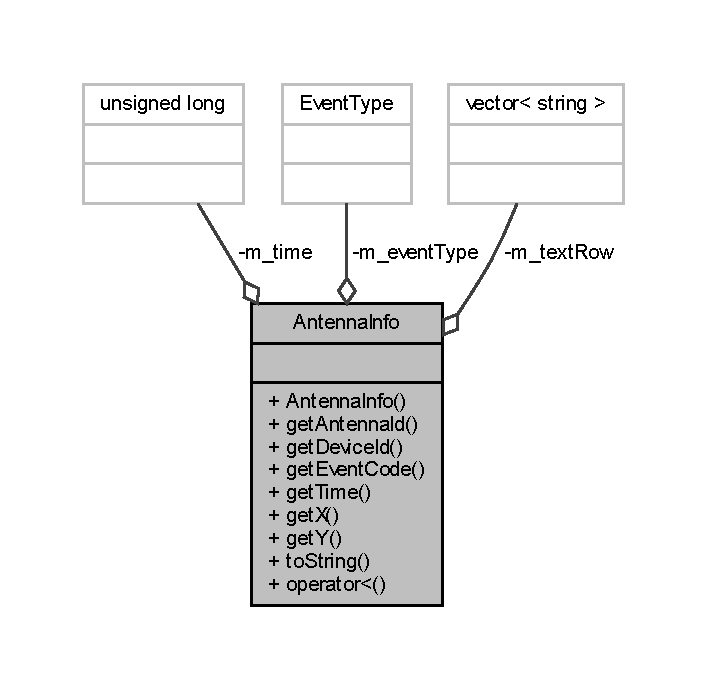
\includegraphics[width=340pt]{class_antenna_info__coll__graph}
\end{center}
\end{figure}
\doxysubsection*{Public Member Functions}
\begin{DoxyCompactItemize}
\item 
\mbox{\hyperlink{class_antenna_info_a4cbcbed39618d71c76ab72b777b4d849}{Antenna\+Info}} (\mbox{\hyperlink{_event_type_8h_a2628ea8d12e8b2563c32f05dc7fff6fa}{Event\+Type}} evt\+Type, \mbox{\hyperlink{class_row}{Row}} r)
\item 
const unsigned long \mbox{\hyperlink{class_antenna_info_a551235c9dca1231beedda388a36280a5}{get\+Antenna\+Id}} () const
\item 
const unsigned long \mbox{\hyperlink{class_antenna_info_ae59a012bda35bb1ccfe1ff2c4038ac18}{get\+Device\+Id}} () const
\item 
const unsigned long \mbox{\hyperlink{class_antenna_info_a300f601af4e815890b385e661f43c335}{get\+Event\+Code}} () const
\item 
unsigned long \mbox{\hyperlink{class_antenna_info_aaae1e1105ba4a724c0061e3f7904b1e5}{get\+Time}} () const
\item 
double \mbox{\hyperlink{class_antenna_info_a3817cba0231888dc5977105ace0faddb}{getX}} () const
\item 
double \mbox{\hyperlink{class_antenna_info_aa385e3e85d783b81d69014a64b5fc94f}{getY}} () const
\item 
const string \mbox{\hyperlink{class_antenna_info_ae1ba7432ca7aef9a4f79a422ee195a58}{to\+String}} () const
\item 
bool \mbox{\hyperlink{class_antenna_info_a74156652eb5ad9a62f41fea726e33b40}{operator$<$}} (const \mbox{\hyperlink{class_antenna_info}{Antenna\+Info}} \&ai) const
\end{DoxyCompactItemize}
\doxysubsection*{Private Attributes}
\begin{DoxyCompactItemize}
\item 
\mbox{\hyperlink{_event_type_8h_a2628ea8d12e8b2563c32f05dc7fff6fa}{Event\+Type}} \mbox{\hyperlink{class_antenna_info_aae043083f5d58b4d7264be468b45541a}{m\+\_\+event\+Type}}
\item 
unsigned long \mbox{\hyperlink{class_antenna_info_a355d929c83040e154f635ce149286b05}{m\+\_\+time}}
\item 
vector$<$ string $>$ \mbox{\hyperlink{class_antenna_info_a46f54626284418436f65f03718e8d38e}{m\+\_\+text\+Row}}
\end{DoxyCompactItemize}


\doxysubsection{Detailed Description}
This class is used to encapsulate all the information about an event generated by an antenna\+: the timestamp, antenna\+Id, event code, the device id, the exact location of the event. 

\doxysubsection{Constructor \& Destructor Documentation}
\mbox{\Hypertarget{class_antenna_info_a4cbcbed39618d71c76ab72b777b4d849}\label{class_antenna_info_a4cbcbed39618d71c76ab72b777b4d849}} 
\index{AntennaInfo@{AntennaInfo}!AntennaInfo@{AntennaInfo}}
\index{AntennaInfo@{AntennaInfo}!AntennaInfo@{AntennaInfo}}
\doxysubsubsection{\texorpdfstring{AntennaInfo()}{AntennaInfo()}}
{\footnotesize\ttfamily Antenna\+Info\+::\+Antenna\+Info (\begin{DoxyParamCaption}\item[{\mbox{\hyperlink{_event_type_8h_a2628ea8d12e8b2563c32f05dc7fff6fa}{Event\+Type}}}]{evt\+Type,  }\item[{\mbox{\hyperlink{class_row}{Row}}}]{r }\end{DoxyParamCaption})}



\doxysubsection{Member Function Documentation}
\mbox{\Hypertarget{class_antenna_info_a551235c9dca1231beedda388a36280a5}\label{class_antenna_info_a551235c9dca1231beedda388a36280a5}} 
\index{AntennaInfo@{AntennaInfo}!getAntennaId@{getAntennaId}}
\index{getAntennaId@{getAntennaId}!AntennaInfo@{AntennaInfo}}
\doxysubsubsection{\texorpdfstring{getAntennaId()}{getAntennaId()}}
{\footnotesize\ttfamily const unsigned long Antenna\+Info\+::get\+Antenna\+Id (\begin{DoxyParamCaption}{ }\end{DoxyParamCaption}) const}

Constructor of the class, builds an object with the values of the fields provided as arguments. 
\begin{DoxyParams}{Parameters}
{\em time} & the timestamp of the event. \\
\hline
{\em antenna\+Id} & the id of the antenna that registered an event. \\
\hline
{\em event} & the event code. \\
\hline
{\em device\+Id} & the id of the device that generated the event. \\
\hline
{\em x} & x coordinate of the device when the event was generated. \\
\hline
{\em y} & y coordinate of the device when the event was generated. \\
\hline
\end{DoxyParams}
\begin{DoxyReturn}{Returns}
the id of the antenna that registered the event. 
\end{DoxyReturn}
\mbox{\Hypertarget{class_antenna_info_ae59a012bda35bb1ccfe1ff2c4038ac18}\label{class_antenna_info_ae59a012bda35bb1ccfe1ff2c4038ac18}} 
\index{AntennaInfo@{AntennaInfo}!getDeviceId@{getDeviceId}}
\index{getDeviceId@{getDeviceId}!AntennaInfo@{AntennaInfo}}
\doxysubsubsection{\texorpdfstring{getDeviceId()}{getDeviceId()}}
{\footnotesize\ttfamily const unsigned long Antenna\+Info\+::get\+Device\+Id (\begin{DoxyParamCaption}{ }\end{DoxyParamCaption}) const}

\begin{DoxyReturn}{Returns}
the id of the device that generated the event. 
\end{DoxyReturn}
\mbox{\Hypertarget{class_antenna_info_a300f601af4e815890b385e661f43c335}\label{class_antenna_info_a300f601af4e815890b385e661f43c335}} 
\index{AntennaInfo@{AntennaInfo}!getEventCode@{getEventCode}}
\index{getEventCode@{getEventCode}!AntennaInfo@{AntennaInfo}}
\doxysubsubsection{\texorpdfstring{getEventCode()}{getEventCode()}}
{\footnotesize\ttfamily const unsigned long Antenna\+Info\+::get\+Event\+Code (\begin{DoxyParamCaption}{ }\end{DoxyParamCaption}) const}

\begin{DoxyReturn}{Returns}
the event code. It could take the following values\+: 0 -\/ a device is connected to an antenna, 1 -\/ a devices is disconnected from an antenna, 2 -\/ a device is already connected to the antenna that registered the event, 3 -\/ a device was detected in the coverage area of an antenna but the connection to the antenna failed (from different reasons). 
\end{DoxyReturn}
\mbox{\Hypertarget{class_antenna_info_aaae1e1105ba4a724c0061e3f7904b1e5}\label{class_antenna_info_aaae1e1105ba4a724c0061e3f7904b1e5}} 
\index{AntennaInfo@{AntennaInfo}!getTime@{getTime}}
\index{getTime@{getTime}!AntennaInfo@{AntennaInfo}}
\doxysubsubsection{\texorpdfstring{getTime()}{getTime()}}
{\footnotesize\ttfamily unsigned long Antenna\+Info\+::get\+Time (\begin{DoxyParamCaption}{ }\end{DoxyParamCaption}) const}

\begin{DoxyReturn}{Returns}
the timestamp of the event. 
\end{DoxyReturn}
\mbox{\Hypertarget{class_antenna_info_a3817cba0231888dc5977105ace0faddb}\label{class_antenna_info_a3817cba0231888dc5977105ace0faddb}} 
\index{AntennaInfo@{AntennaInfo}!getX@{getX}}
\index{getX@{getX}!AntennaInfo@{AntennaInfo}}
\doxysubsubsection{\texorpdfstring{getX()}{getX()}}
{\footnotesize\ttfamily double Antenna\+Info\+::getX (\begin{DoxyParamCaption}{ }\end{DoxyParamCaption}) const}

\begin{DoxyReturn}{Returns}
x coordinate of the device that generated the event. 
\end{DoxyReturn}
\mbox{\Hypertarget{class_antenna_info_aa385e3e85d783b81d69014a64b5fc94f}\label{class_antenna_info_aa385e3e85d783b81d69014a64b5fc94f}} 
\index{AntennaInfo@{AntennaInfo}!getY@{getY}}
\index{getY@{getY}!AntennaInfo@{AntennaInfo}}
\doxysubsubsection{\texorpdfstring{getY()}{getY()}}
{\footnotesize\ttfamily double Antenna\+Info\+::getY (\begin{DoxyParamCaption}{ }\end{DoxyParamCaption}) const}

\begin{DoxyReturn}{Returns}
y coordinate of the device that generated the event. 
\end{DoxyReturn}
\mbox{\Hypertarget{class_antenna_info_a74156652eb5ad9a62f41fea726e33b40}\label{class_antenna_info_a74156652eb5ad9a62f41fea726e33b40}} 
\index{AntennaInfo@{AntennaInfo}!operator$<$@{operator$<$}}
\index{operator$<$@{operator$<$}!AntennaInfo@{AntennaInfo}}
\doxysubsubsection{\texorpdfstring{operator$<$()}{operator<()}}
{\footnotesize\ttfamily bool Antenna\+Info\+::operator$<$ (\begin{DoxyParamCaption}\item[{const \mbox{\hyperlink{class_antenna_info}{Antenna\+Info}} \&}]{ai }\end{DoxyParamCaption}) const}

Overloaded operator to compare to objects 
\begin{DoxyParams}{Parameters}
{\em ai} & the other object to compare to. \\
\hline
\end{DoxyParams}
\begin{DoxyReturn}{Returns}
true if this object is less than ai, false otherwise. An object is less than another object if the timestamp value of the first object is lees than the timestamp of the second one. 
\end{DoxyReturn}
\mbox{\Hypertarget{class_antenna_info_ae1ba7432ca7aef9a4f79a422ee195a58}\label{class_antenna_info_ae1ba7432ca7aef9a4f79a422ee195a58}} 
\index{AntennaInfo@{AntennaInfo}!toString@{toString}}
\index{toString@{toString}!AntennaInfo@{AntennaInfo}}
\doxysubsubsection{\texorpdfstring{toString()}{toString()}}
{\footnotesize\ttfamily const string Antenna\+Info\+::to\+String (\begin{DoxyParamCaption}{ }\end{DoxyParamCaption}) const}

\begin{DoxyReturn}{Returns}
a string representation of on object of this class. 
\end{DoxyReturn}


\doxysubsection{Member Data Documentation}
\mbox{\Hypertarget{class_antenna_info_aae043083f5d58b4d7264be468b45541a}\label{class_antenna_info_aae043083f5d58b4d7264be468b45541a}} 
\index{AntennaInfo@{AntennaInfo}!m\_eventType@{m\_eventType}}
\index{m\_eventType@{m\_eventType}!AntennaInfo@{AntennaInfo}}
\doxysubsubsection{\texorpdfstring{m\_eventType}{m\_eventType}}
{\footnotesize\ttfamily \mbox{\hyperlink{_event_type_8h_a2628ea8d12e8b2563c32f05dc7fff6fa}{Event\+Type}} Antenna\+Info\+::m\+\_\+event\+Type\hspace{0.3cm}{\ttfamily [private]}}

\mbox{\Hypertarget{class_antenna_info_a46f54626284418436f65f03718e8d38e}\label{class_antenna_info_a46f54626284418436f65f03718e8d38e}} 
\index{AntennaInfo@{AntennaInfo}!m\_textRow@{m\_textRow}}
\index{m\_textRow@{m\_textRow}!AntennaInfo@{AntennaInfo}}
\doxysubsubsection{\texorpdfstring{m\_textRow}{m\_textRow}}
{\footnotesize\ttfamily vector$<$string$>$ Antenna\+Info\+::m\+\_\+text\+Row\hspace{0.3cm}{\ttfamily [private]}}

\mbox{\Hypertarget{class_antenna_info_a355d929c83040e154f635ce149286b05}\label{class_antenna_info_a355d929c83040e154f635ce149286b05}} 
\index{AntennaInfo@{AntennaInfo}!m\_time@{m\_time}}
\index{m\_time@{m\_time}!AntennaInfo@{AntennaInfo}}
\doxysubsubsection{\texorpdfstring{m\_time}{m\_time}}
{\footnotesize\ttfamily unsigned long Antenna\+Info\+::m\+\_\+time\hspace{0.3cm}{\ttfamily [private]}}



The documentation for this class was generated from the following file\+:\begin{DoxyCompactItemize}
\item 
include/\mbox{\hyperlink{_antenna_info_8h}{Antenna\+Info.\+h}}\end{DoxyCompactItemize}

\hypertarget{class_clock}{}\section{Clock Class Reference}
\label{class_clock}\index{Clock@{Clock}}


{\ttfamily \#include $<$Clock.\+h$>$}



Collaboration diagram for Clock\+:\nopagebreak
\begin{figure}[H]
\begin{center}
\leavevmode
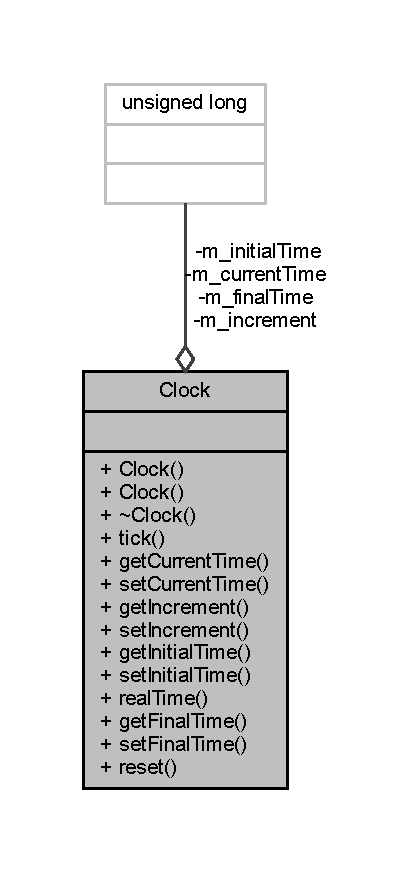
\includegraphics[width=197pt]{class_clock__coll__graph}
\end{center}
\end{figure}
\subsection*{Public Member Functions}
\begin{DoxyCompactItemize}
\item 
\hyperlink{class_clock_adbc370eb6b5f8d01645cf440188160a8}{Clock} ()
\item 
\hyperlink{class_clock_a89a798e152f8eba2f6eb80ec92b26ece}{Clock} (unsigned long start, unsigned long end, unsigned long incr)
\item 
virtual \hyperlink{class_clock_ac1ddbca9092c61e98668473209f36b19}{$\sim$\+Clock} ()
\item 
unsigned long \hyperlink{class_clock_ab7c857c5b43cf98d991435ba9ce46b2c}{tick} ()
\item 
unsigned long \hyperlink{class_clock_a17b19c062d1f0344f37b57cc2dfdaa14}{get\+Current\+Time} () const
\item 
void \hyperlink{class_clock_a7046e8733ab749d3c24b3c61bd108d6c}{set\+Current\+Time} (unsigned long current\+Time)
\item 
unsigned long \hyperlink{class_clock_a804626d5455f4a2a73321f84ed7a9819}{get\+Increment} () const
\item 
void \hyperlink{class_clock_a1ae60dca4e41f6e27d6104ec618c02f1}{set\+Increment} (unsigned long increment)
\item 
unsigned long \hyperlink{class_clock_a9792f62fed3c320abecc5c455b13a804}{get\+Initial\+Time} () const
\item 
void \hyperlink{class_clock_abe7fb8f715d0dcae08e52b2b7aed7db2}{set\+Initial\+Time} (unsigned long initial\+Time)
\item 
time\+\_\+t \hyperlink{class_clock_a29512d39298cafed334d0c01da70ea7b}{real\+Time} ()
\item 
unsigned long \hyperlink{class_clock_a0b9ef0b9272d6555bb0fdca4978c705d}{get\+Final\+Time} () const
\item 
void \hyperlink{class_clock_a4780f83b55bc2539cd7069cfc4f06d99}{set\+Final\+Time} (unsigned long final\+Time)
\item 
void \hyperlink{class_clock_a0ab5423b0a997aa13d7b6131c46d1358}{reset} ()
\end{DoxyCompactItemize}
\subsection*{Private Attributes}
\begin{DoxyCompactItemize}
\item 
unsigned long \hyperlink{class_clock_a71afbea0f41f612e36d45ee2bb79ff0e}{m\+\_\+initial\+Time}
\item 
unsigned long \hyperlink{class_clock_a73bf4edfc8f0fe2548ef6956f68b678e}{m\+\_\+current\+Time}
\item 
unsigned long \hyperlink{class_clock_a2f940f0a30d58d1f7f36d0296463b9aa}{m\+\_\+increment}
\item 
unsigned long \hyperlink{class_clock_a5c473d84c1051d946ab5565060902840}{m\+\_\+final\+Time}
\end{DoxyCompactItemize}


\subsection{Detailed Description}
This is the clock used to synchronize the simulation. All the agents and all other objects involved in a simulation use the same \hyperlink{class_clock}{Clock} object. The \hyperlink{class_clock}{Clock} will be initialized with the value of the starting and ending time of the simulation and will keep a current time during the simulation. At each step of the simulation the current time will be increased by an increment. Starting time, ending time, current time and the time increment are only conventional units and they do not depend in any way on the real clock of the computer. 

\subsection{Constructor \& Destructor Documentation}
\mbox{\Hypertarget{class_clock_adbc370eb6b5f8d01645cf440188160a8}\label{class_clock_adbc370eb6b5f8d01645cf440188160a8}} 
\index{Clock@{Clock}!Clock@{Clock}}
\index{Clock@{Clock}!Clock@{Clock}}
\subsubsection{\texorpdfstring{Clock()}{Clock()}\hspace{0.1cm}{\footnotesize\ttfamily [1/2]}}
{\footnotesize\ttfamily Clock\+::\+Clock (\begin{DoxyParamCaption}{ }\end{DoxyParamCaption})}

Default constructor \mbox{\Hypertarget{class_clock_a89a798e152f8eba2f6eb80ec92b26ece}\label{class_clock_a89a798e152f8eba2f6eb80ec92b26ece}} 
\index{Clock@{Clock}!Clock@{Clock}}
\index{Clock@{Clock}!Clock@{Clock}}
\subsubsection{\texorpdfstring{Clock()}{Clock()}\hspace{0.1cm}{\footnotesize\ttfamily [2/2]}}
{\footnotesize\ttfamily Clock\+::\+Clock (\begin{DoxyParamCaption}\item[{unsigned long}]{start,  }\item[{unsigned long}]{end,  }\item[{unsigned long}]{incr }\end{DoxyParamCaption})}

Constructor of the class. It takes the starting and ending time of the simulation as parameters as well as the time increment. 
\begin{DoxyParams}{Parameters}
{\em start} & the initial moment when the simulation starts. \\
\hline
{\em end} & the time when simulation ends. \\
\hline
{\em incr} & the time increment. At each step of the simulation the current time is incremented by this quantity. \\
\hline
\end{DoxyParams}
\mbox{\Hypertarget{class_clock_ac1ddbca9092c61e98668473209f36b19}\label{class_clock_ac1ddbca9092c61e98668473209f36b19}} 
\index{Clock@{Clock}!````~Clock@{$\sim$\+Clock}}
\index{````~Clock@{$\sim$\+Clock}!Clock@{Clock}}
\subsubsection{\texorpdfstring{$\sim$\+Clock()}{~Clock()}}
{\footnotesize\ttfamily virtual Clock\+::$\sim$\+Clock (\begin{DoxyParamCaption}{ }\end{DoxyParamCaption})\hspace{0.3cm}{\ttfamily [virtual]}}

Default destructor 

\subsection{Member Function Documentation}
\mbox{\Hypertarget{class_clock_a17b19c062d1f0344f37b57cc2dfdaa14}\label{class_clock_a17b19c062d1f0344f37b57cc2dfdaa14}} 
\index{Clock@{Clock}!get\+Current\+Time@{get\+Current\+Time}}
\index{get\+Current\+Time@{get\+Current\+Time}!Clock@{Clock}}
\subsubsection{\texorpdfstring{get\+Current\+Time()}{getCurrentTime()}}
{\footnotesize\ttfamily unsigned long Clock\+::get\+Current\+Time (\begin{DoxyParamCaption}{ }\end{DoxyParamCaption}) const}

\begin{DoxyReturn}{Returns}
the current time of the simulator. 
\end{DoxyReturn}
\mbox{\Hypertarget{class_clock_a0b9ef0b9272d6555bb0fdca4978c705d}\label{class_clock_a0b9ef0b9272d6555bb0fdca4978c705d}} 
\index{Clock@{Clock}!get\+Final\+Time@{get\+Final\+Time}}
\index{get\+Final\+Time@{get\+Final\+Time}!Clock@{Clock}}
\subsubsection{\texorpdfstring{get\+Final\+Time()}{getFinalTime()}}
{\footnotesize\ttfamily unsigned long Clock\+::get\+Final\+Time (\begin{DoxyParamCaption}{ }\end{DoxyParamCaption}) const}

\begin{DoxyReturn}{Returns}
the ending time of the simulation. 
\end{DoxyReturn}
\mbox{\Hypertarget{class_clock_a804626d5455f4a2a73321f84ed7a9819}\label{class_clock_a804626d5455f4a2a73321f84ed7a9819}} 
\index{Clock@{Clock}!get\+Increment@{get\+Increment}}
\index{get\+Increment@{get\+Increment}!Clock@{Clock}}
\subsubsection{\texorpdfstring{get\+Increment()}{getIncrement()}}
{\footnotesize\ttfamily unsigned long Clock\+::get\+Increment (\begin{DoxyParamCaption}{ }\end{DoxyParamCaption}) const}

\begin{DoxyReturn}{Returns}
the time increment used in simulation. 
\end{DoxyReturn}
\mbox{\Hypertarget{class_clock_a9792f62fed3c320abecc5c455b13a804}\label{class_clock_a9792f62fed3c320abecc5c455b13a804}} 
\index{Clock@{Clock}!get\+Initial\+Time@{get\+Initial\+Time}}
\index{get\+Initial\+Time@{get\+Initial\+Time}!Clock@{Clock}}
\subsubsection{\texorpdfstring{get\+Initial\+Time()}{getInitialTime()}}
{\footnotesize\ttfamily unsigned long Clock\+::get\+Initial\+Time (\begin{DoxyParamCaption}{ }\end{DoxyParamCaption}) const}

\begin{DoxyReturn}{Returns}
the starting time of the simulation. 
\end{DoxyReturn}
\mbox{\Hypertarget{class_clock_a29512d39298cafed334d0c01da70ea7b}\label{class_clock_a29512d39298cafed334d0c01da70ea7b}} 
\index{Clock@{Clock}!real\+Time@{real\+Time}}
\index{real\+Time@{real\+Time}!Clock@{Clock}}
\subsubsection{\texorpdfstring{real\+Time()}{realTime()}}
{\footnotesize\ttfamily time\+\_\+t Clock\+::real\+Time (\begin{DoxyParamCaption}{ }\end{DoxyParamCaption})}

\begin{DoxyReturn}{Returns}
the real time read from the computer clock. It is used only to register the exact date and time of a simulation. 
\end{DoxyReturn}
\mbox{\Hypertarget{class_clock_a0ab5423b0a997aa13d7b6131c46d1358}\label{class_clock_a0ab5423b0a997aa13d7b6131c46d1358}} 
\index{Clock@{Clock}!reset@{reset}}
\index{reset@{reset}!Clock@{Clock}}
\subsubsection{\texorpdfstring{reset()}{reset()}}
{\footnotesize\ttfamily void Clock\+::reset (\begin{DoxyParamCaption}{ }\end{DoxyParamCaption})}

Resets the current time and makes it equal to the starting time such that a new simulation can begin. \mbox{\Hypertarget{class_clock_a7046e8733ab749d3c24b3c61bd108d6c}\label{class_clock_a7046e8733ab749d3c24b3c61bd108d6c}} 
\index{Clock@{Clock}!set\+Current\+Time@{set\+Current\+Time}}
\index{set\+Current\+Time@{set\+Current\+Time}!Clock@{Clock}}
\subsubsection{\texorpdfstring{set\+Current\+Time()}{setCurrentTime()}}
{\footnotesize\ttfamily void Clock\+::set\+Current\+Time (\begin{DoxyParamCaption}\item[{unsigned long}]{current\+Time }\end{DoxyParamCaption})}

Sets the current time of the simulator. 
\begin{DoxyParams}{Parameters}
{\em current\+Time} & the value of the current time to be set. \\
\hline
\end{DoxyParams}
\mbox{\Hypertarget{class_clock_a4780f83b55bc2539cd7069cfc4f06d99}\label{class_clock_a4780f83b55bc2539cd7069cfc4f06d99}} 
\index{Clock@{Clock}!set\+Final\+Time@{set\+Final\+Time}}
\index{set\+Final\+Time@{set\+Final\+Time}!Clock@{Clock}}
\subsubsection{\texorpdfstring{set\+Final\+Time()}{setFinalTime()}}
{\footnotesize\ttfamily void Clock\+::set\+Final\+Time (\begin{DoxyParamCaption}\item[{unsigned long}]{final\+Time }\end{DoxyParamCaption})}

Sets the ending time of a simulation. 
\begin{DoxyParams}{Parameters}
{\em final\+Time} & the value of the ending time of a simulation. \\
\hline
\end{DoxyParams}
\mbox{\Hypertarget{class_clock_a1ae60dca4e41f6e27d6104ec618c02f1}\label{class_clock_a1ae60dca4e41f6e27d6104ec618c02f1}} 
\index{Clock@{Clock}!set\+Increment@{set\+Increment}}
\index{set\+Increment@{set\+Increment}!Clock@{Clock}}
\subsubsection{\texorpdfstring{set\+Increment()}{setIncrement()}}
{\footnotesize\ttfamily void Clock\+::set\+Increment (\begin{DoxyParamCaption}\item[{unsigned long}]{increment }\end{DoxyParamCaption})}

Sets the time increment to be used in a simulation. 
\begin{DoxyParams}{Parameters}
{\em increment} & the value of the time increment. \\
\hline
\end{DoxyParams}
\mbox{\Hypertarget{class_clock_abe7fb8f715d0dcae08e52b2b7aed7db2}\label{class_clock_abe7fb8f715d0dcae08e52b2b7aed7db2}} 
\index{Clock@{Clock}!set\+Initial\+Time@{set\+Initial\+Time}}
\index{set\+Initial\+Time@{set\+Initial\+Time}!Clock@{Clock}}
\subsubsection{\texorpdfstring{set\+Initial\+Time()}{setInitialTime()}}
{\footnotesize\ttfamily void Clock\+::set\+Initial\+Time (\begin{DoxyParamCaption}\item[{unsigned long}]{initial\+Time }\end{DoxyParamCaption})}

Sets the starting time of the simulation. 
\begin{DoxyParams}{Parameters}
{\em initial\+Time} & the value of the starting time of the simulation. \\
\hline
\end{DoxyParams}
\mbox{\Hypertarget{class_clock_ab7c857c5b43cf98d991435ba9ce46b2c}\label{class_clock_ab7c857c5b43cf98d991435ba9ce46b2c}} 
\index{Clock@{Clock}!tick@{tick}}
\index{tick@{tick}!Clock@{Clock}}
\subsubsection{\texorpdfstring{tick()}{tick()}}
{\footnotesize\ttfamily unsigned long Clock\+::tick (\begin{DoxyParamCaption}{ }\end{DoxyParamCaption})}

increments the current time. \begin{DoxyReturn}{Returns}
the current time after incrementation. 
\end{DoxyReturn}


\subsection{Member Data Documentation}
\mbox{\Hypertarget{class_clock_a73bf4edfc8f0fe2548ef6956f68b678e}\label{class_clock_a73bf4edfc8f0fe2548ef6956f68b678e}} 
\index{Clock@{Clock}!m\+\_\+current\+Time@{m\+\_\+current\+Time}}
\index{m\+\_\+current\+Time@{m\+\_\+current\+Time}!Clock@{Clock}}
\subsubsection{\texorpdfstring{m\+\_\+current\+Time}{m\_currentTime}}
{\footnotesize\ttfamily unsigned long Clock\+::m\+\_\+current\+Time\hspace{0.3cm}{\ttfamily [private]}}

\mbox{\Hypertarget{class_clock_a5c473d84c1051d946ab5565060902840}\label{class_clock_a5c473d84c1051d946ab5565060902840}} 
\index{Clock@{Clock}!m\+\_\+final\+Time@{m\+\_\+final\+Time}}
\index{m\+\_\+final\+Time@{m\+\_\+final\+Time}!Clock@{Clock}}
\subsubsection{\texorpdfstring{m\+\_\+final\+Time}{m\_finalTime}}
{\footnotesize\ttfamily unsigned long Clock\+::m\+\_\+final\+Time\hspace{0.3cm}{\ttfamily [private]}}

\mbox{\Hypertarget{class_clock_a2f940f0a30d58d1f7f36d0296463b9aa}\label{class_clock_a2f940f0a30d58d1f7f36d0296463b9aa}} 
\index{Clock@{Clock}!m\+\_\+increment@{m\+\_\+increment}}
\index{m\+\_\+increment@{m\+\_\+increment}!Clock@{Clock}}
\subsubsection{\texorpdfstring{m\+\_\+increment}{m\_increment}}
{\footnotesize\ttfamily unsigned long Clock\+::m\+\_\+increment\hspace{0.3cm}{\ttfamily [private]}}

\mbox{\Hypertarget{class_clock_a71afbea0f41f612e36d45ee2bb79ff0e}\label{class_clock_a71afbea0f41f612e36d45ee2bb79ff0e}} 
\index{Clock@{Clock}!m\+\_\+initial\+Time@{m\+\_\+initial\+Time}}
\index{m\+\_\+initial\+Time@{m\+\_\+initial\+Time}!Clock@{Clock}}
\subsubsection{\texorpdfstring{m\+\_\+initial\+Time}{m\_initialTime}}
{\footnotesize\ttfamily unsigned long Clock\+::m\+\_\+initial\+Time\hspace{0.3cm}{\ttfamily [private]}}



The documentation for this class was generated from the following file\+:\begin{DoxyCompactItemize}
\item 
include/\hyperlink{_clock_8h}{Clock.\+h}\end{DoxyCompactItemize}

\hypertarget{class_config_parser}{}\doxysection{Config\+Parser Class Reference}
\label{class_config_parser}\index{ConfigParser@{ConfigParser}}


{\ttfamily \#include $<$Config\+Parser.\+h$>$}



Inheritance diagram for Config\+Parser\+:
\nopagebreak
\begin{figure}[H]
\begin{center}
\leavevmode
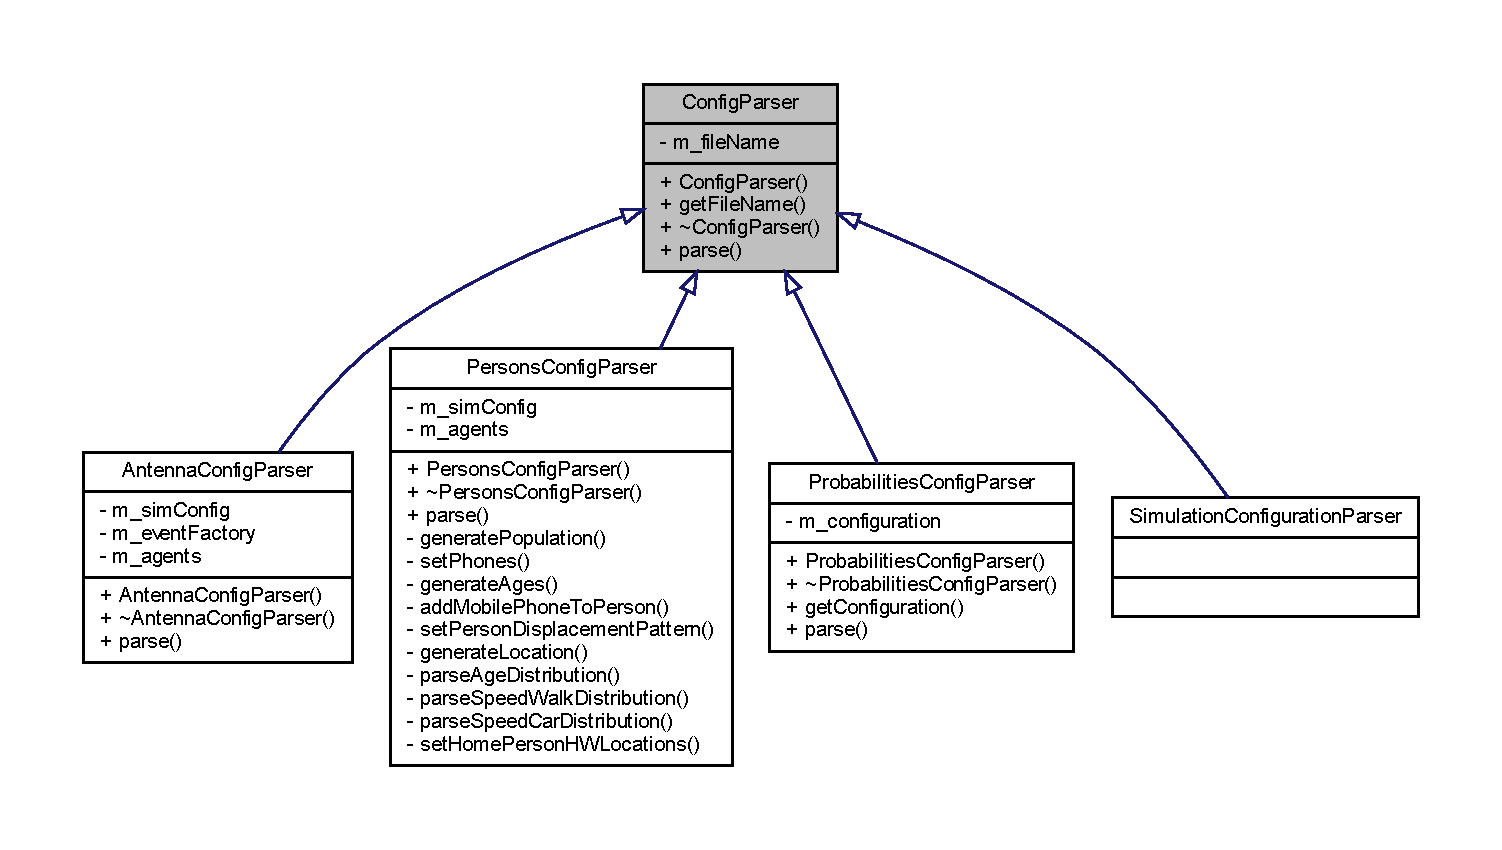
\includegraphics[width=350pt]{class_config_parser__inherit__graph}
\end{center}
\end{figure}


Collaboration diagram for Config\+Parser\+:
\nopagebreak
\begin{figure}[H]
\begin{center}
\leavevmode
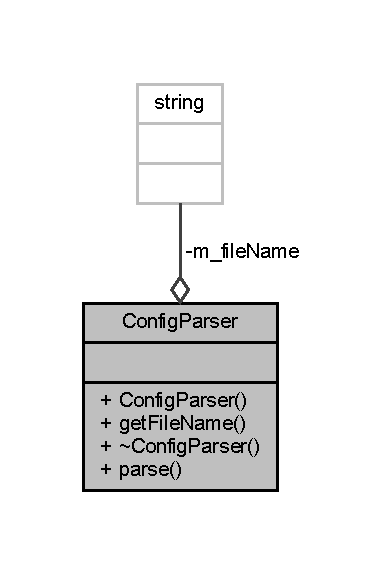
\includegraphics[width=185pt]{class_config_parser__coll__graph}
\end{center}
\end{figure}
\doxysubsection*{Public Member Functions}
\begin{DoxyCompactItemize}
\item 
\mbox{\hyperlink{class_config_parser_a1fab78cfa555b0ae67a6255923bbc0d9}{Config\+Parser}} (string file\+Name)
\item 
string \mbox{\hyperlink{class_config_parser_a51c01f04f57685d476a6b1d64809eeaa}{get\+File\+Name}} () const
\item 
virtual \mbox{\hyperlink{class_config_parser_a610d3e5316be803c8f1bb7eebe32504b}{$\sim$\+Config\+Parser}} ()
\item 
virtual void \mbox{\hyperlink{class_config_parser_afc13df32c129e923c7aa33db7413dd2e}{parse}} ()=0
\end{DoxyCompactItemize}
\doxysubsection*{Private Attributes}
\begin{DoxyCompactItemize}
\item 
string \mbox{\hyperlink{class_config_parser_a9fe6ed9463012eeb23b3fb62b1a51f84}{m\+\_\+file\+Name}}
\end{DoxyCompactItemize}


\doxysubsection{Detailed Description}
The base class for the configuration file parsers. All derived classes handle a specific type of configuration file\+: simulation, persons, antennas, probabilities. These derived classes parse the corresponding configuration file, build the corresponding objects (\mbox{\hyperlink{class_antenna}{Antenna}}, \mbox{\hyperlink{class_person}{Person}}, \mbox{\hyperlink{class_mobile_phone}{Mobile\+Phone}}, \mbox{\hyperlink{class_mobile_operator}{Mobile\+Operator}}) and add them to the \mbox{\hyperlink{class_agents_collection}{Agents\+Collection}} container. This is an abstract class, it contains one pure virtual function, \mbox{\hyperlink{class_config_parser_afc13df32c129e923c7aa33db7413dd2e}{parse()}} that has to be implemented by subclasses. 

\doxysubsection{Constructor \& Destructor Documentation}
\mbox{\Hypertarget{class_config_parser_a1fab78cfa555b0ae67a6255923bbc0d9}\label{class_config_parser_a1fab78cfa555b0ae67a6255923bbc0d9}} 
\index{ConfigParser@{ConfigParser}!ConfigParser@{ConfigParser}}
\index{ConfigParser@{ConfigParser}!ConfigParser@{ConfigParser}}
\doxysubsubsection{\texorpdfstring{ConfigParser()}{ConfigParser()}}
{\footnotesize\ttfamily Config\+Parser\+::\+Config\+Parser (\begin{DoxyParamCaption}\item[{string}]{file\+Name }\end{DoxyParamCaption})}

Constructor of the class. It takes the filename of the configuration file as a parameter and stores it internally. 
\begin{DoxyParams}{Parameters}
{\em file\+Name} & the name of configuration file to be parsed. \\
\hline
\end{DoxyParams}
\mbox{\Hypertarget{class_config_parser_a610d3e5316be803c8f1bb7eebe32504b}\label{class_config_parser_a610d3e5316be803c8f1bb7eebe32504b}} 
\index{ConfigParser@{ConfigParser}!````~ConfigParser@{$\sim$ConfigParser}}
\index{````~ConfigParser@{$\sim$ConfigParser}!ConfigParser@{ConfigParser}}
\doxysubsubsection{\texorpdfstring{$\sim$ConfigParser()}{~ConfigParser()}}
{\footnotesize\ttfamily virtual Config\+Parser\+::$\sim$\+Config\+Parser (\begin{DoxyParamCaption}{ }\end{DoxyParamCaption})\hspace{0.3cm}{\ttfamily [virtual]}}

Virtual destructor of the class. 

\doxysubsection{Member Function Documentation}
\mbox{\Hypertarget{class_config_parser_a51c01f04f57685d476a6b1d64809eeaa}\label{class_config_parser_a51c01f04f57685d476a6b1d64809eeaa}} 
\index{ConfigParser@{ConfigParser}!getFileName@{getFileName}}
\index{getFileName@{getFileName}!ConfigParser@{ConfigParser}}
\doxysubsubsection{\texorpdfstring{getFileName()}{getFileName()}}
{\footnotesize\ttfamily string Config\+Parser\+::get\+File\+Name (\begin{DoxyParamCaption}{ }\end{DoxyParamCaption}) const}

Returns the name of the configuration file. \begin{DoxyReturn}{Returns}
the name of the configuration file. 
\end{DoxyReturn}
\mbox{\Hypertarget{class_config_parser_afc13df32c129e923c7aa33db7413dd2e}\label{class_config_parser_afc13df32c129e923c7aa33db7413dd2e}} 
\index{ConfigParser@{ConfigParser}!parse@{parse}}
\index{parse@{parse}!ConfigParser@{ConfigParser}}
\doxysubsubsection{\texorpdfstring{parse()}{parse()}}
{\footnotesize\ttfamily virtual void Config\+Parser\+::parse (\begin{DoxyParamCaption}{ }\end{DoxyParamCaption})\hspace{0.3cm}{\ttfamily [pure virtual]}}

This pure virtual function has to be implemented by specific subclasses. Each subclass will be specialized to parse one of the configuration file used by the simulation software\+: simulation, persons, antennas, probabilities. They are passed in the command line of the software using the \char`\"{}-\/s\char`\"{}, \char`\"{}-\/p\char`\"{}, \char`\"{}-\/a\char`\"{}, \char`\"{}-\/pb\char`\"{} options. 

Implemented in \mbox{\hyperlink{class_antenna_config_parser_a19b457a8adbecb36dc97b2449dae76c9}{Antenna\+Config\+Parser}}, \mbox{\hyperlink{class_probabilities_config_parser_ad330952ebf080070f9407d829ca99dcd}{Probabilities\+Config\+Parser}}, and \mbox{\hyperlink{class_persons_config_parser_a4141c4d5506894a98dd0c05810c987a4}{Persons\+Config\+Parser}}.



\doxysubsection{Member Data Documentation}
\mbox{\Hypertarget{class_config_parser_a9fe6ed9463012eeb23b3fb62b1a51f84}\label{class_config_parser_a9fe6ed9463012eeb23b3fb62b1a51f84}} 
\index{ConfigParser@{ConfigParser}!m\_fileName@{m\_fileName}}
\index{m\_fileName@{m\_fileName}!ConfigParser@{ConfigParser}}
\doxysubsubsection{\texorpdfstring{m\_fileName}{m\_fileName}}
{\footnotesize\ttfamily string Config\+Parser\+::m\+\_\+file\+Name\hspace{0.3cm}{\ttfamily [private]}}



The documentation for this class was generated from the following file\+:\begin{DoxyCompactItemize}
\item 
include/parsers/\mbox{\hyperlink{_config_parser_8h}{Config\+Parser.\+h}}\end{DoxyCompactItemize}

\hypertarget{class_constants}{}\doxysection{Constants Class Reference}
\label{class_constants}\index{Constants@{Constants}}


{\ttfamily \#include $<$Constants.\+h$>$}



Collaboration diagram for Constants\+:\nopagebreak
\begin{figure}[H]
\begin{center}
\leavevmode
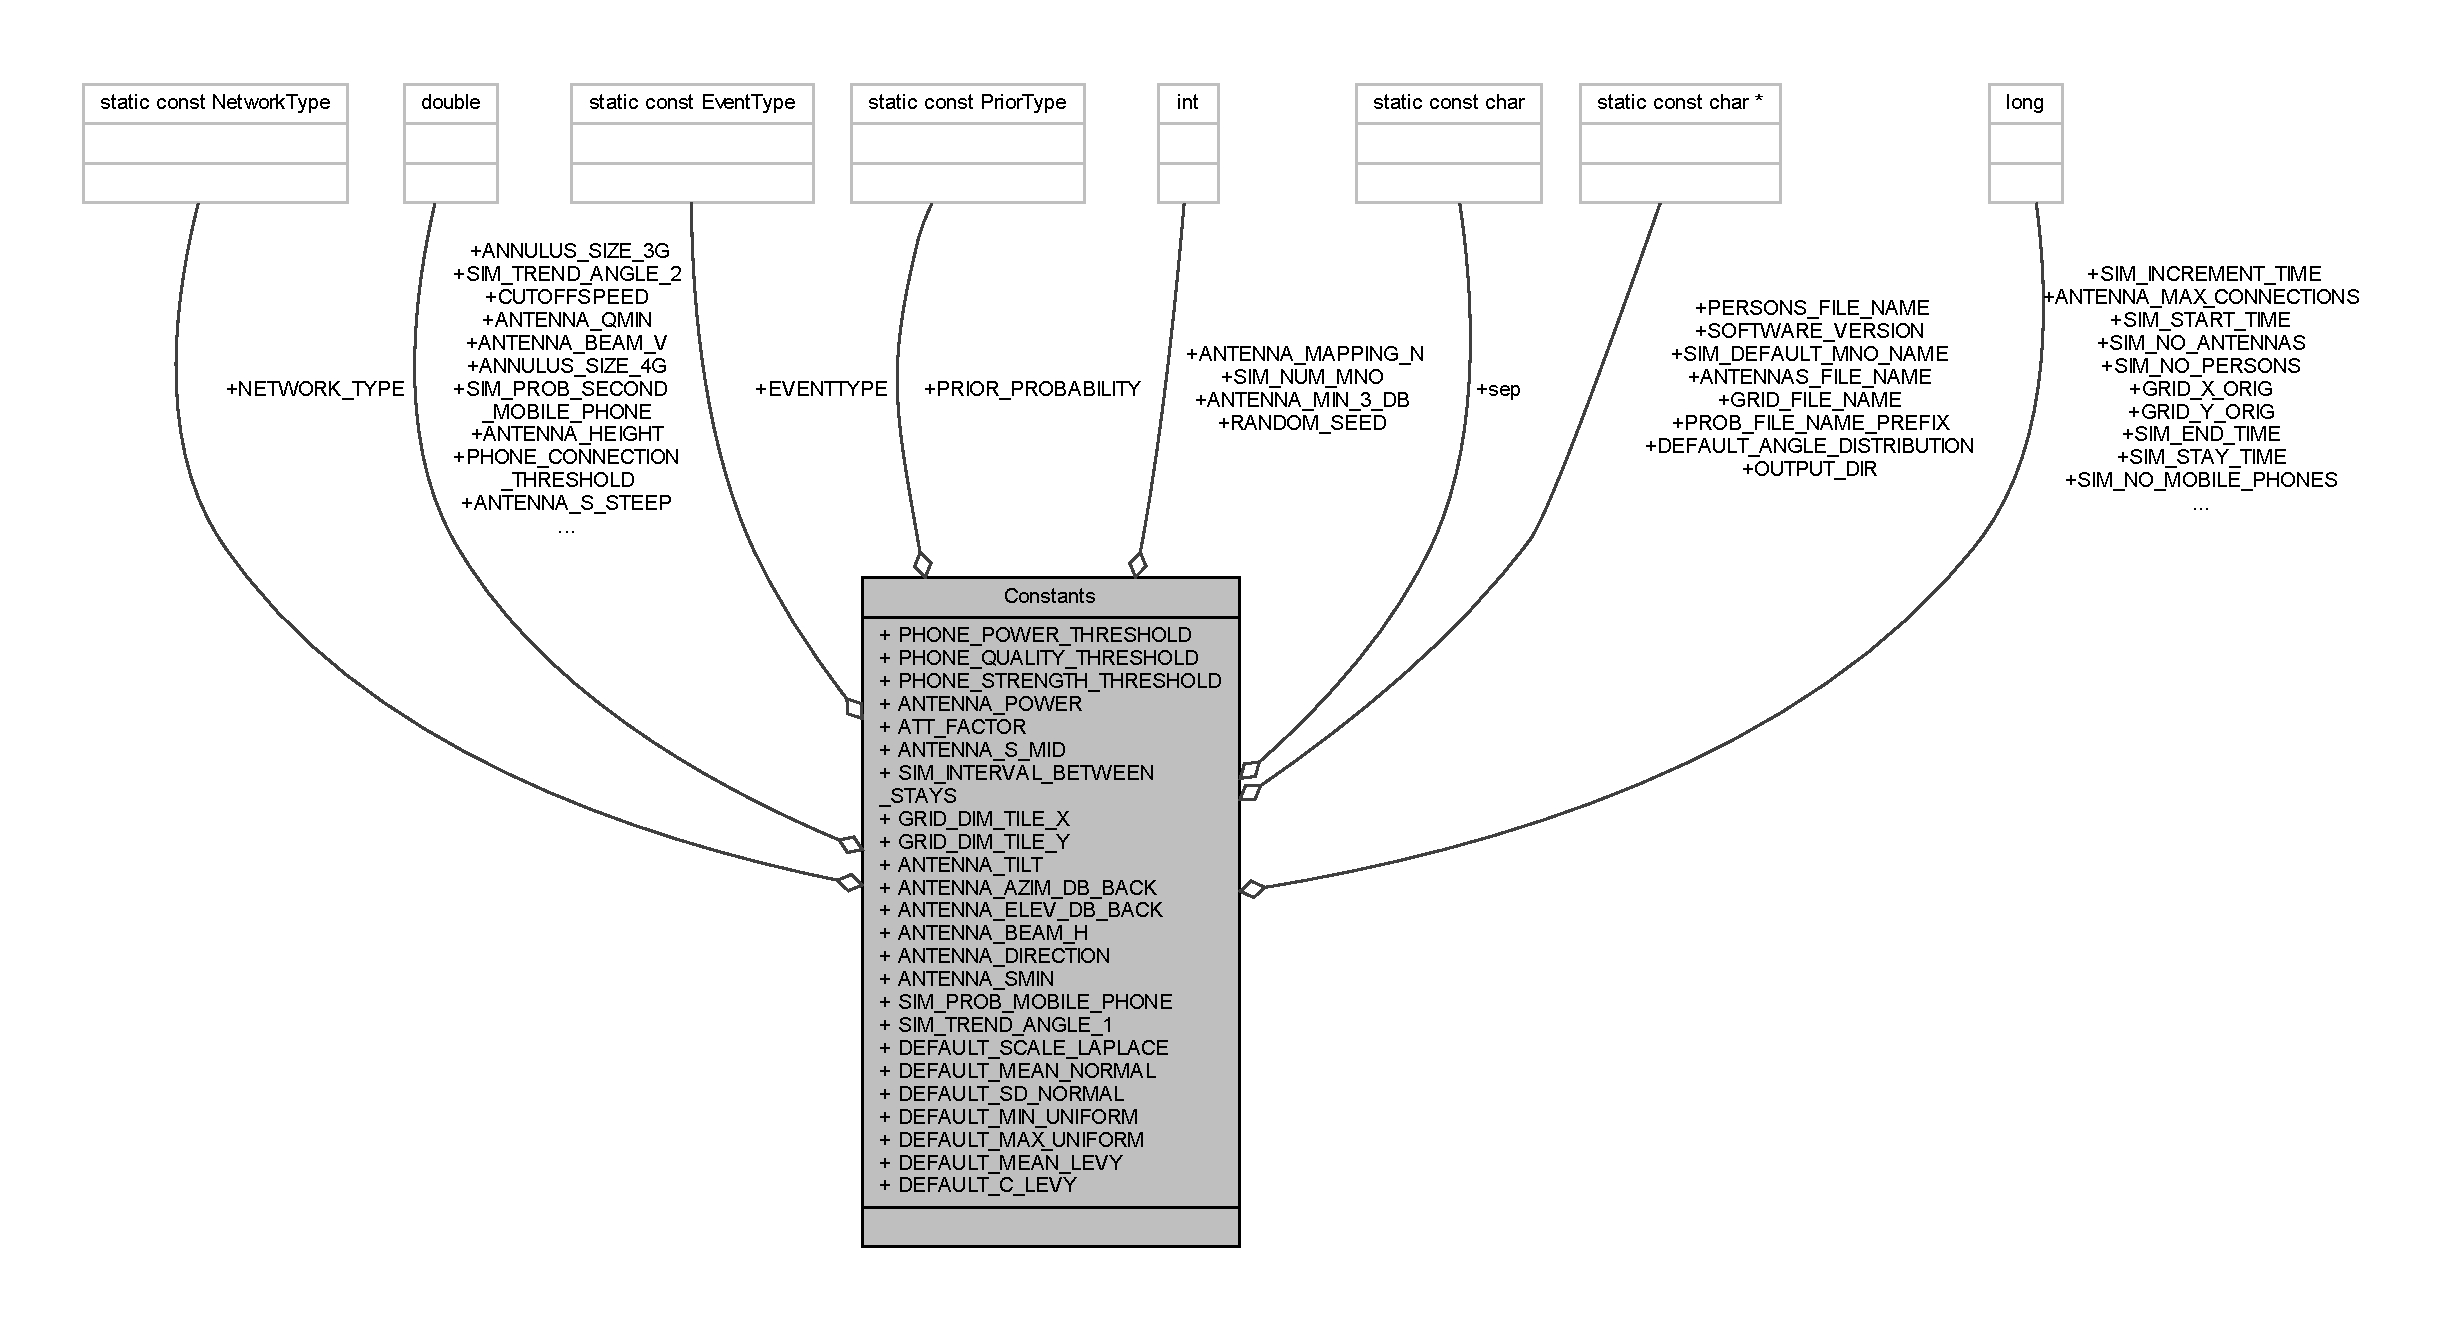
\includegraphics[width=350pt]{class_constants__coll__graph}
\end{center}
\end{figure}
\doxysubsection*{Static Public Attributes}
\begin{DoxyCompactItemize}
\item 
static const double \mbox{\hyperlink{class_constants_a1e95cbdc2db02f6147ddf8ac61a428ab}{P\+H\+O\+N\+E\+\_\+\+P\+O\+W\+E\+R\+\_\+\+T\+H\+R\+E\+S\+H\+O\+LD}}
\item 
static const double \mbox{\hyperlink{class_constants_a2c8a9d965bae29c19ff18c8b80260982}{P\+H\+O\+N\+E\+\_\+\+Q\+U\+A\+L\+I\+T\+Y\+\_\+\+T\+H\+R\+E\+S\+H\+O\+LD}}
\item 
static const double \mbox{\hyperlink{class_constants_a24b6069c3365fb95c4b853129e4d4a3e}{P\+H\+O\+N\+E\+\_\+\+S\+T\+R\+E\+N\+G\+T\+H\+\_\+\+T\+H\+R\+E\+S\+H\+O\+LD}}
\item 
static const double \mbox{\hyperlink{class_constants_a1cbf0a4e111b9d2e13b33e771a342b4f}{P\+H\+O\+N\+E\+\_\+\+C\+O\+N\+N\+E\+C\+T\+I\+O\+N\+\_\+\+T\+H\+R\+E\+S\+H\+O\+LD}}
\item 
static const double \mbox{\hyperlink{class_constants_a3f6f3825098d8eb1dc8081158c46c48a}{A\+N\+T\+E\+N\+N\+A\+\_\+\+P\+O\+W\+ER}}
\item 
static const double \mbox{\hyperlink{class_constants_a3738ccd4e7931b93885bdedf98528293}{A\+T\+T\+\_\+\+F\+A\+C\+T\+OR}}
\item 
static const unsigned long \mbox{\hyperlink{class_constants_af89a10a7d59ac020b1fa06cf673ef01f}{A\+N\+T\+E\+N\+N\+A\+\_\+\+M\+A\+X\+\_\+\+C\+O\+N\+N\+E\+C\+T\+I\+O\+NS}}
\item 
static const double \mbox{\hyperlink{class_constants_aea09e28749c0da58a4c831f9eabea773}{A\+N\+T\+E\+N\+N\+A\+\_\+\+S\+\_\+\+M\+ID}}
\item 
static const double \mbox{\hyperlink{class_constants_ae4b1b2c15d1e5bbb76464c03036c6baa}{A\+N\+T\+E\+N\+N\+A\+\_\+\+S\+\_\+\+S\+T\+E\+EP}}
\item 
static const unsigned long \mbox{\hyperlink{class_constants_a627fe53a717da1ca017b2467fb1dd4df}{S\+I\+M\+\_\+\+N\+O\+\_\+\+P\+E\+R\+S\+O\+NS}}
\item 
static const unsigned long \mbox{\hyperlink{class_constants_a0f6bc08399ad62727732e08a65c3bd0f}{S\+I\+M\+\_\+\+N\+O\+\_\+\+A\+N\+T\+E\+N\+N\+AS}}
\item 
static const unsigned long \mbox{\hyperlink{class_constants_a7da9e25a998c58c4388cbd45411f4232}{S\+I\+M\+\_\+\+N\+O\+\_\+\+M\+O\+B\+I\+L\+E\+\_\+\+P\+H\+O\+N\+ES}}
\item 
static const unsigned long \mbox{\hyperlink{class_constants_ad8a2d4817d599fd4f608e474bf1052ba}{S\+I\+M\+\_\+\+S\+T\+A\+R\+T\+\_\+\+T\+I\+ME}}
\item 
static const unsigned long \mbox{\hyperlink{class_constants_affb253c69b40f5979cd07383245331b7}{S\+I\+M\+\_\+\+E\+N\+D\+\_\+\+T\+I\+ME}}
\item 
static const unsigned long \mbox{\hyperlink{class_constants_ae689749614ecdd38b50a014400138bc2}{S\+I\+M\+\_\+\+I\+N\+C\+R\+E\+M\+E\+N\+T\+\_\+\+T\+I\+ME}}
\item 
static const unsigned long \mbox{\hyperlink{class_constants_a885a54aa8b2d13632ae3e8ff8e7664fb}{S\+I\+M\+\_\+\+S\+T\+A\+Y\+\_\+\+T\+I\+ME}}
\item 
static const unsigned long \mbox{\hyperlink{class_constants_a396cc1e9abbdf0a536886ebfd6b28045}{S\+I\+M\+\_\+\+I\+N\+T\+E\+R\+V\+A\+L\+\_\+\+B\+E\+T\+W\+E\+E\+N\+\_\+\+S\+T\+A\+YS}}
\item 
static const char \mbox{\hyperlink{class_constants_afc927f63cc5fbb912114d6b0f28b8b4f}{sep}}
\item 
static const char $\ast$ \mbox{\hyperlink{class_constants_aa2fd1c5551c8dab10dc1bd4c0cd0db8f}{G\+R\+I\+D\+\_\+\+F\+I\+L\+E\+\_\+\+N\+A\+ME}}
\item 
static const unsigned long \mbox{\hyperlink{class_constants_ac09062322e1ab9b6e1ca3a568b11c376}{G\+R\+I\+D\+\_\+\+X\+\_\+\+O\+R\+IG}}
\item 
static const unsigned long \mbox{\hyperlink{class_constants_ace48b30468931aaf452ab7a6daf573e0}{G\+R\+I\+D\+\_\+\+Y\+\_\+\+O\+R\+IG}}
\item 
static const double \mbox{\hyperlink{class_constants_a4400d3f97fa2e2be6091a8005efedd7f}{G\+R\+I\+D\+\_\+\+D\+I\+M\+\_\+\+T\+I\+L\+E\+\_\+X}}
\item 
static const double \mbox{\hyperlink{class_constants_a08f9273d844b68a74fd979d5a46d4918}{G\+R\+I\+D\+\_\+\+D\+I\+M\+\_\+\+T\+I\+L\+E\+\_\+Y}}
\item 
static const char $\ast$ \mbox{\hyperlink{class_constants_a3b2d3fc0ccc4636a51190bf5b297d72d}{P\+R\+O\+B\+\_\+\+F\+I\+L\+E\+\_\+\+N\+A\+M\+E\+\_\+\+P\+R\+E\+F\+IX}}
\item 
static const char $\ast$ \mbox{\hyperlink{class_constants_a2388516c40960223c0aef1610fd72312}{P\+E\+R\+S\+O\+N\+S\+\_\+\+F\+I\+L\+E\+\_\+\+N\+A\+ME}}
\item 
static const char $\ast$ \mbox{\hyperlink{class_constants_a23f758b23b88c7cfe23b278647671acb}{A\+N\+T\+E\+N\+N\+A\+S\+\_\+\+F\+I\+L\+E\+\_\+\+N\+A\+ME}}
\item 
static const char $\ast$ \mbox{\hyperlink{class_constants_a91fc37386abce571a0c7cd3f1b4b47c3}{O\+U\+T\+P\+U\+T\+\_\+\+D\+IR}}
\item 
static const \mbox{\hyperlink{_prior_type_8h_a61286c562e68de246982fc393a7c23a5}{Prior\+Type}} \mbox{\hyperlink{class_constants_a7b31976adc7ad0f3dbed86b205e1773d}{P\+R\+I\+O\+R\+\_\+\+P\+R\+O\+B\+A\+B\+I\+L\+I\+TY}}
\item 
static const \mbox{\hyperlink{_network_type_8h_a3a159600500d5d7248be5bd1ca1f8d83}{Network\+Type}} \mbox{\hyperlink{class_constants_acdce90461fcc403b55fcbd846b32c3b8}{N\+E\+T\+W\+O\+R\+K\+\_\+\+T\+Y\+PE}}
\item 
static const double \mbox{\hyperlink{class_constants_adfe27efa61ae50b73c74b3f19c292625}{A\+N\+T\+E\+N\+N\+A\+\_\+\+H\+E\+I\+G\+HT}}
\item 
static const double \mbox{\hyperlink{class_constants_ad92a5c99071f0d843ee555e74c5f909a}{A\+N\+T\+E\+N\+N\+A\+\_\+\+T\+I\+LT}}
\item 
static const double \mbox{\hyperlink{class_constants_aa2030f2c0ec89fb7cc06b31bbb50793d}{A\+N\+T\+E\+N\+N\+A\+\_\+\+A\+Z\+I\+M\+\_\+\+D\+B\+\_\+\+B\+A\+CK}}
\item 
static const double \mbox{\hyperlink{class_constants_a8efdd6e1f2a25c24cb6dbff363e2d61a}{A\+N\+T\+E\+N\+N\+A\+\_\+\+E\+L\+E\+V\+\_\+\+D\+B\+\_\+\+B\+A\+CK}}
\item 
static const double \mbox{\hyperlink{class_constants_a4e4a0a48ad06c458ae4f3e6d0e4e6608}{A\+N\+T\+E\+N\+N\+A\+\_\+\+B\+E\+A\+M\+\_\+H}}
\item 
static const double \mbox{\hyperlink{class_constants_a2389355f6184d3b7903e154b46d069f5}{A\+N\+T\+E\+N\+N\+A\+\_\+\+B\+E\+A\+M\+\_\+V}}
\item 
static const double \mbox{\hyperlink{class_constants_ad82a10e13ae9e1cbce1cef616e47df31}{A\+N\+T\+E\+N\+N\+A\+\_\+\+D\+I\+R\+E\+C\+T\+I\+ON}}
\item 
static const unsigned int \mbox{\hyperlink{class_constants_a5db3a5bad9c514c994e71063dee2a798}{A\+N\+T\+E\+N\+N\+A\+\_\+\+M\+A\+P\+P\+I\+N\+G\+\_\+N}}
\item 
static const unsigned int \mbox{\hyperlink{class_constants_a2bda61c04e204f4a1279338fb790e1f4}{A\+N\+T\+E\+N\+N\+A\+\_\+\+M\+I\+N\+\_\+3\+\_\+\+DB}}
\item 
static const double \mbox{\hyperlink{class_constants_af58b693e1ab4cdb1e83399eb0f2af647}{A\+N\+T\+E\+N\+N\+A\+\_\+\+S\+M\+IN}}
\item 
static const double \mbox{\hyperlink{class_constants_a9149aaac071422191e4417885fd42b07}{A\+N\+T\+E\+N\+N\+A\+\_\+\+Q\+M\+IN}}
\item 
static const unsigned int \mbox{\hyperlink{class_constants_a763bdd9401295d6b691c93cf580e562a}{S\+I\+M\+\_\+\+N\+U\+M\+\_\+\+M\+NO}}
\item 
static const char $\ast$ \mbox{\hyperlink{class_constants_a186cf83e20074a889823a7f36e50ad8c}{S\+I\+M\+\_\+\+D\+E\+F\+A\+U\+L\+T\+\_\+\+M\+N\+O\+\_\+\+N\+A\+ME}}
\item 
static const double \mbox{\hyperlink{class_constants_a8af75c6e731c2f425cce792b33786db7}{S\+I\+M\+\_\+\+P\+R\+O\+B\+\_\+\+M\+O\+B\+I\+L\+E\+\_\+\+P\+H\+O\+NE}}
\item 
static const double \mbox{\hyperlink{class_constants_aafd39df52173dca1074d8c92aa5f9649}{S\+I\+M\+\_\+\+P\+R\+O\+B\+\_\+\+S\+E\+C\+O\+N\+D\+\_\+\+M\+O\+B\+I\+L\+E\+\_\+\+P\+H\+O\+NE}}
\item 
static const double \mbox{\hyperlink{class_constants_a97968377c9a3cf2995c37aa63d3dd505}{S\+I\+M\+\_\+\+T\+R\+E\+N\+D\+\_\+\+A\+N\+G\+L\+E\+\_\+1}}
\item 
static const double \mbox{\hyperlink{class_constants_a1ec9cdffb9c58a2ff1cb60f64b056835}{S\+I\+M\+\_\+\+T\+R\+E\+N\+D\+\_\+\+A\+N\+G\+L\+E\+\_\+2}}
\item 
static const int \mbox{\hyperlink{class_constants_ac80eccfaa8e498ad3fc6ea0a2c3d38a0}{R\+A\+N\+D\+O\+M\+\_\+\+S\+E\+ED}}
\item 
static const double \mbox{\hyperlink{class_constants_a66de7fc72fc30ccf2599816cf607c14c}{A\+N\+N\+U\+L\+U\+S\+\_\+\+S\+I\+Z\+E\+\_\+3G}}
\item 
static const double \mbox{\hyperlink{class_constants_a8ff3d2e927af8b78332fcf1d72891fc7}{A\+N\+N\+U\+L\+U\+S\+\_\+\+S\+I\+Z\+E\+\_\+4G}}
\item 
static const char $\ast$ \mbox{\hyperlink{class_constants_a6049bf9f7258073e70696221b0fc5b3a}{S\+O\+F\+T\+W\+A\+R\+E\+\_\+\+V\+E\+R\+S\+I\+ON}}
\item 
static const \mbox{\hyperlink{_event_type_8h_a2628ea8d12e8b2563c32f05dc7fff6fa}{Event\+Type}} \mbox{\hyperlink{class_constants_a10eced3c79b838621f744eb1ca0b1195}{E\+V\+E\+N\+T\+T\+Y\+PE}}
\item 
static const char $\ast$ \mbox{\hyperlink{class_constants_a5c160562a1c7a4b6fb42be9c8ab51fa2}{D\+E\+F\+A\+U\+L\+T\+\_\+\+A\+N\+G\+L\+E\+\_\+\+D\+I\+S\+T\+R\+I\+B\+U\+T\+I\+ON}}
\item 
static const double \mbox{\hyperlink{class_constants_a8b08b468ea38caf46e4f1f4ef27065ce}{D\+E\+F\+A\+U\+L\+T\+\_\+\+S\+C\+A\+L\+E\+\_\+\+L\+A\+P\+L\+A\+CE}}
\item 
static const double \mbox{\hyperlink{class_constants_ac1dc5a89a1de331d8dabd10bc88f1a79}{D\+E\+F\+A\+U\+L\+T\+\_\+\+M\+E\+A\+N\+\_\+\+N\+O\+R\+M\+AL}}
\item 
static const double \mbox{\hyperlink{class_constants_ac950a1666ca87477d83b2ca5efdbbf66}{D\+E\+F\+A\+U\+L\+T\+\_\+\+S\+D\+\_\+\+N\+O\+R\+M\+AL}}
\item 
static const double \mbox{\hyperlink{class_constants_ac795990b722ff47dd0fdf06638c57dd6}{D\+E\+F\+A\+U\+L\+T\+\_\+\+M\+I\+N\+\_\+\+U\+N\+I\+F\+O\+RM}}
\item 
static const double \mbox{\hyperlink{class_constants_a8a4671c81f16a6952a2533e983befc93}{D\+E\+F\+A\+U\+L\+T\+\_\+\+M\+A\+X\+\_\+\+U\+N\+I\+F\+O\+RM}}
\item 
static const double \mbox{\hyperlink{class_constants_a62ab8ab582731606c42f264b53fc3e69}{C\+U\+T\+O\+F\+F\+S\+P\+E\+ED}}
\item 
static const double \mbox{\hyperlink{class_constants_a375dbd64a60179f9fcaf1c7b7606bad6}{D\+E\+F\+A\+U\+L\+T\+\_\+\+M\+E\+A\+N\+\_\+\+L\+E\+VY}}
\item 
static const double \mbox{\hyperlink{class_constants_a942c5242af9de9d6545e690268450c03}{D\+E\+F\+A\+U\+L\+T\+\_\+\+C\+\_\+\+L\+E\+VY}}
\end{DoxyCompactItemize}


\doxysubsection{Detailed Description}
These are some constants used in the process of the simulation, most of them are only used for testing and rapid development of some methods, the real values of the parameters being read from the configuration files. 

\doxysubsection{Member Data Documentation}
\mbox{\Hypertarget{class_constants_a66de7fc72fc30ccf2599816cf607c14c}\label{class_constants_a66de7fc72fc30ccf2599816cf607c14c}} 
\index{Constants@{Constants}!ANNULUS\_SIZE\_3G@{ANNULUS\_SIZE\_3G}}
\index{ANNULUS\_SIZE\_3G@{ANNULUS\_SIZE\_3G}!Constants@{Constants}}
\doxysubsubsection{\texorpdfstring{ANNULUS\_SIZE\_3G}{ANNULUS\_SIZE\_3G}}
{\footnotesize\ttfamily const double Constants\+::\+A\+N\+N\+U\+L\+U\+S\+\_\+\+S\+I\+Z\+E\+\_\+3G\hspace{0.3cm}{\ttfamily [static]}}

\mbox{\Hypertarget{class_constants_a8ff3d2e927af8b78332fcf1d72891fc7}\label{class_constants_a8ff3d2e927af8b78332fcf1d72891fc7}} 
\index{Constants@{Constants}!ANNULUS\_SIZE\_4G@{ANNULUS\_SIZE\_4G}}
\index{ANNULUS\_SIZE\_4G@{ANNULUS\_SIZE\_4G}!Constants@{Constants}}
\doxysubsubsection{\texorpdfstring{ANNULUS\_SIZE\_4G}{ANNULUS\_SIZE\_4G}}
{\footnotesize\ttfamily const double Constants\+::\+A\+N\+N\+U\+L\+U\+S\+\_\+\+S\+I\+Z\+E\+\_\+4G\hspace{0.3cm}{\ttfamily [static]}}

\mbox{\Hypertarget{class_constants_aa2030f2c0ec89fb7cc06b31bbb50793d}\label{class_constants_aa2030f2c0ec89fb7cc06b31bbb50793d}} 
\index{Constants@{Constants}!ANTENNA\_AZIM\_DB\_BACK@{ANTENNA\_AZIM\_DB\_BACK}}
\index{ANTENNA\_AZIM\_DB\_BACK@{ANTENNA\_AZIM\_DB\_BACK}!Constants@{Constants}}
\doxysubsubsection{\texorpdfstring{ANTENNA\_AZIM\_DB\_BACK}{ANTENNA\_AZIM\_DB\_BACK}}
{\footnotesize\ttfamily const double Constants\+::\+A\+N\+T\+E\+N\+N\+A\+\_\+\+A\+Z\+I\+M\+\_\+\+D\+B\+\_\+\+B\+A\+CK\hspace{0.3cm}{\ttfamily [static]}}

\mbox{\Hypertarget{class_constants_a4e4a0a48ad06c458ae4f3e6d0e4e6608}\label{class_constants_a4e4a0a48ad06c458ae4f3e6d0e4e6608}} 
\index{Constants@{Constants}!ANTENNA\_BEAM\_H@{ANTENNA\_BEAM\_H}}
\index{ANTENNA\_BEAM\_H@{ANTENNA\_BEAM\_H}!Constants@{Constants}}
\doxysubsubsection{\texorpdfstring{ANTENNA\_BEAM\_H}{ANTENNA\_BEAM\_H}}
{\footnotesize\ttfamily const double Constants\+::\+A\+N\+T\+E\+N\+N\+A\+\_\+\+B\+E\+A\+M\+\_\+H\hspace{0.3cm}{\ttfamily [static]}}

\mbox{\Hypertarget{class_constants_a2389355f6184d3b7903e154b46d069f5}\label{class_constants_a2389355f6184d3b7903e154b46d069f5}} 
\index{Constants@{Constants}!ANTENNA\_BEAM\_V@{ANTENNA\_BEAM\_V}}
\index{ANTENNA\_BEAM\_V@{ANTENNA\_BEAM\_V}!Constants@{Constants}}
\doxysubsubsection{\texorpdfstring{ANTENNA\_BEAM\_V}{ANTENNA\_BEAM\_V}}
{\footnotesize\ttfamily const double Constants\+::\+A\+N\+T\+E\+N\+N\+A\+\_\+\+B\+E\+A\+M\+\_\+V\hspace{0.3cm}{\ttfamily [static]}}

\mbox{\Hypertarget{class_constants_ad82a10e13ae9e1cbce1cef616e47df31}\label{class_constants_ad82a10e13ae9e1cbce1cef616e47df31}} 
\index{Constants@{Constants}!ANTENNA\_DIRECTION@{ANTENNA\_DIRECTION}}
\index{ANTENNA\_DIRECTION@{ANTENNA\_DIRECTION}!Constants@{Constants}}
\doxysubsubsection{\texorpdfstring{ANTENNA\_DIRECTION}{ANTENNA\_DIRECTION}}
{\footnotesize\ttfamily const double Constants\+::\+A\+N\+T\+E\+N\+N\+A\+\_\+\+D\+I\+R\+E\+C\+T\+I\+ON\hspace{0.3cm}{\ttfamily [static]}}

\mbox{\Hypertarget{class_constants_a8efdd6e1f2a25c24cb6dbff363e2d61a}\label{class_constants_a8efdd6e1f2a25c24cb6dbff363e2d61a}} 
\index{Constants@{Constants}!ANTENNA\_ELEV\_DB\_BACK@{ANTENNA\_ELEV\_DB\_BACK}}
\index{ANTENNA\_ELEV\_DB\_BACK@{ANTENNA\_ELEV\_DB\_BACK}!Constants@{Constants}}
\doxysubsubsection{\texorpdfstring{ANTENNA\_ELEV\_DB\_BACK}{ANTENNA\_ELEV\_DB\_BACK}}
{\footnotesize\ttfamily const double Constants\+::\+A\+N\+T\+E\+N\+N\+A\+\_\+\+E\+L\+E\+V\+\_\+\+D\+B\+\_\+\+B\+A\+CK\hspace{0.3cm}{\ttfamily [static]}}

\mbox{\Hypertarget{class_constants_adfe27efa61ae50b73c74b3f19c292625}\label{class_constants_adfe27efa61ae50b73c74b3f19c292625}} 
\index{Constants@{Constants}!ANTENNA\_HEIGHT@{ANTENNA\_HEIGHT}}
\index{ANTENNA\_HEIGHT@{ANTENNA\_HEIGHT}!Constants@{Constants}}
\doxysubsubsection{\texorpdfstring{ANTENNA\_HEIGHT}{ANTENNA\_HEIGHT}}
{\footnotesize\ttfamily const double Constants\+::\+A\+N\+T\+E\+N\+N\+A\+\_\+\+H\+E\+I\+G\+HT\hspace{0.3cm}{\ttfamily [static]}}

the antenna height \mbox{\Hypertarget{class_constants_a5db3a5bad9c514c994e71063dee2a798}\label{class_constants_a5db3a5bad9c514c994e71063dee2a798}} 
\index{Constants@{Constants}!ANTENNA\_MAPPING\_N@{ANTENNA\_MAPPING\_N}}
\index{ANTENNA\_MAPPING\_N@{ANTENNA\_MAPPING\_N}!Constants@{Constants}}
\doxysubsubsection{\texorpdfstring{ANTENNA\_MAPPING\_N}{ANTENNA\_MAPPING\_N}}
{\footnotesize\ttfamily const unsigned int Constants\+::\+A\+N\+T\+E\+N\+N\+A\+\_\+\+M\+A\+P\+P\+I\+N\+G\+\_\+N\hspace{0.3cm}{\ttfamily [static]}}

\mbox{\Hypertarget{class_constants_af89a10a7d59ac020b1fa06cf673ef01f}\label{class_constants_af89a10a7d59ac020b1fa06cf673ef01f}} 
\index{Constants@{Constants}!ANTENNA\_MAX\_CONNECTIONS@{ANTENNA\_MAX\_CONNECTIONS}}
\index{ANTENNA\_MAX\_CONNECTIONS@{ANTENNA\_MAX\_CONNECTIONS}!Constants@{Constants}}
\doxysubsubsection{\texorpdfstring{ANTENNA\_MAX\_CONNECTIONS}{ANTENNA\_MAX\_CONNECTIONS}}
{\footnotesize\ttfamily const unsigned long Constants\+::\+A\+N\+T\+E\+N\+N\+A\+\_\+\+M\+A\+X\+\_\+\+C\+O\+N\+N\+E\+C\+T\+I\+O\+NS\hspace{0.3cm}{\ttfamily [static]}}

The maximum number of devices an antenna can connect. \mbox{\Hypertarget{class_constants_a2bda61c04e204f4a1279338fb790e1f4}\label{class_constants_a2bda61c04e204f4a1279338fb790e1f4}} 
\index{Constants@{Constants}!ANTENNA\_MIN\_3\_DB@{ANTENNA\_MIN\_3\_DB}}
\index{ANTENNA\_MIN\_3\_DB@{ANTENNA\_MIN\_3\_DB}!Constants@{Constants}}
\doxysubsubsection{\texorpdfstring{ANTENNA\_MIN\_3\_DB}{ANTENNA\_MIN\_3\_DB}}
{\footnotesize\ttfamily const unsigned int Constants\+::\+A\+N\+T\+E\+N\+N\+A\+\_\+\+M\+I\+N\+\_\+3\+\_\+\+DB\hspace{0.3cm}{\ttfamily [static]}}

\mbox{\Hypertarget{class_constants_a3f6f3825098d8eb1dc8081158c46c48a}\label{class_constants_a3f6f3825098d8eb1dc8081158c46c48a}} 
\index{Constants@{Constants}!ANTENNA\_POWER@{ANTENNA\_POWER}}
\index{ANTENNA\_POWER@{ANTENNA\_POWER}!Constants@{Constants}}
\doxysubsubsection{\texorpdfstring{ANTENNA\_POWER}{ANTENNA\_POWER}}
{\footnotesize\ttfamily const double Constants\+::\+A\+N\+T\+E\+N\+N\+A\+\_\+\+P\+O\+W\+ER\hspace{0.3cm}{\ttfamily [static]}}

\mbox{\hyperlink{class_antenna}{Antenna}} power in Watts. \mbox{\Hypertarget{class_constants_a9149aaac071422191e4417885fd42b07}\label{class_constants_a9149aaac071422191e4417885fd42b07}} 
\index{Constants@{Constants}!ANTENNA\_QMIN@{ANTENNA\_QMIN}}
\index{ANTENNA\_QMIN@{ANTENNA\_QMIN}!Constants@{Constants}}
\doxysubsubsection{\texorpdfstring{ANTENNA\_QMIN}{ANTENNA\_QMIN}}
{\footnotesize\ttfamily const double Constants\+::\+A\+N\+T\+E\+N\+N\+A\+\_\+\+Q\+M\+IN\hspace{0.3cm}{\ttfamily [static]}}

\mbox{\Hypertarget{class_constants_aea09e28749c0da58a4c831f9eabea773}\label{class_constants_aea09e28749c0da58a4c831f9eabea773}} 
\index{Constants@{Constants}!ANTENNA\_S\_MID@{ANTENNA\_S\_MID}}
\index{ANTENNA\_S\_MID@{ANTENNA\_S\_MID}!Constants@{Constants}}
\doxysubsubsection{\texorpdfstring{ANTENNA\_S\_MID}{ANTENNA\_S\_MID}}
{\footnotesize\ttfamily const double Constants\+::\+A\+N\+T\+E\+N\+N\+A\+\_\+\+S\+\_\+\+M\+ID\hspace{0.3cm}{\ttfamily [static]}}

The Smid parameter of an antenna \mbox{\Hypertarget{class_constants_ae4b1b2c15d1e5bbb76464c03036c6baa}\label{class_constants_ae4b1b2c15d1e5bbb76464c03036c6baa}} 
\index{Constants@{Constants}!ANTENNA\_S\_STEEP@{ANTENNA\_S\_STEEP}}
\index{ANTENNA\_S\_STEEP@{ANTENNA\_S\_STEEP}!Constants@{Constants}}
\doxysubsubsection{\texorpdfstring{ANTENNA\_S\_STEEP}{ANTENNA\_S\_STEEP}}
{\footnotesize\ttfamily const double Constants\+::\+A\+N\+T\+E\+N\+N\+A\+\_\+\+S\+\_\+\+S\+T\+E\+EP\hspace{0.3cm}{\ttfamily [static]}}

The Sstepp parameter of an antenna \mbox{\Hypertarget{class_constants_af58b693e1ab4cdb1e83399eb0f2af647}\label{class_constants_af58b693e1ab4cdb1e83399eb0f2af647}} 
\index{Constants@{Constants}!ANTENNA\_SMIN@{ANTENNA\_SMIN}}
\index{ANTENNA\_SMIN@{ANTENNA\_SMIN}!Constants@{Constants}}
\doxysubsubsection{\texorpdfstring{ANTENNA\_SMIN}{ANTENNA\_SMIN}}
{\footnotesize\ttfamily const double Constants\+::\+A\+N\+T\+E\+N\+N\+A\+\_\+\+S\+M\+IN\hspace{0.3cm}{\ttfamily [static]}}

\mbox{\Hypertarget{class_constants_ad92a5c99071f0d843ee555e74c5f909a}\label{class_constants_ad92a5c99071f0d843ee555e74c5f909a}} 
\index{Constants@{Constants}!ANTENNA\_TILT@{ANTENNA\_TILT}}
\index{ANTENNA\_TILT@{ANTENNA\_TILT}!Constants@{Constants}}
\doxysubsubsection{\texorpdfstring{ANTENNA\_TILT}{ANTENNA\_TILT}}
{\footnotesize\ttfamily const double Constants\+::\+A\+N\+T\+E\+N\+N\+A\+\_\+\+T\+I\+LT\hspace{0.3cm}{\ttfamily [static]}}

\mbox{\Hypertarget{class_constants_a23f758b23b88c7cfe23b278647671acb}\label{class_constants_a23f758b23b88c7cfe23b278647671acb}} 
\index{Constants@{Constants}!ANTENNAS\_FILE\_NAME@{ANTENNAS\_FILE\_NAME}}
\index{ANTENNAS\_FILE\_NAME@{ANTENNAS\_FILE\_NAME}!Constants@{Constants}}
\doxysubsubsection{\texorpdfstring{ANTENNAS\_FILE\_NAME}{ANTENNAS\_FILE\_NAME}}
{\footnotesize\ttfamily const char$\ast$ Constants\+::\+A\+N\+T\+E\+N\+N\+A\+S\+\_\+\+F\+I\+L\+E\+\_\+\+N\+A\+ME\hspace{0.3cm}{\ttfamily [static]}}

The name of the file where the exact positions of the antennas are saved during simulation. They are needed for later analysis. \mbox{\Hypertarget{class_constants_a3738ccd4e7931b93885bdedf98528293}\label{class_constants_a3738ccd4e7931b93885bdedf98528293}} 
\index{Constants@{Constants}!ATT\_FACTOR@{ATT\_FACTOR}}
\index{ATT\_FACTOR@{ATT\_FACTOR}!Constants@{Constants}}
\doxysubsubsection{\texorpdfstring{ATT\_FACTOR}{ATT\_FACTOR}}
{\footnotesize\ttfamily const double Constants\+::\+A\+T\+T\+\_\+\+F\+A\+C\+T\+OR\hspace{0.3cm}{\ttfamily [static]}}

Attenuation factor of the signal. It usually takes values between 2 in open field and 6 inside buildings \mbox{\Hypertarget{class_constants_a62ab8ab582731606c42f264b53fc3e69}\label{class_constants_a62ab8ab582731606c42f264b53fc3e69}} 
\index{Constants@{Constants}!CUTOFFSPEED@{CUTOFFSPEED}}
\index{CUTOFFSPEED@{CUTOFFSPEED}!Constants@{Constants}}
\doxysubsubsection{\texorpdfstring{CUTOFFSPEED}{CUTOFFSPEED}}
{\footnotesize\ttfamily const double Constants\+::\+C\+U\+T\+O\+F\+F\+S\+P\+E\+ED\hspace{0.3cm}{\ttfamily [static]}}

\mbox{\Hypertarget{class_constants_a5c160562a1c7a4b6fb42be9c8ab51fa2}\label{class_constants_a5c160562a1c7a4b6fb42be9c8ab51fa2}} 
\index{Constants@{Constants}!DEFAULT\_ANGLE\_DISTRIBUTION@{DEFAULT\_ANGLE\_DISTRIBUTION}}
\index{DEFAULT\_ANGLE\_DISTRIBUTION@{DEFAULT\_ANGLE\_DISTRIBUTION}!Constants@{Constants}}
\doxysubsubsection{\texorpdfstring{DEFAULT\_ANGLE\_DISTRIBUTION}{DEFAULT\_ANGLE\_DISTRIBUTION}}
{\footnotesize\ttfamily const char$\ast$ Constants\+::\+D\+E\+F\+A\+U\+L\+T\+\_\+\+A\+N\+G\+L\+E\+\_\+\+D\+I\+S\+T\+R\+I\+B\+U\+T\+I\+ON\hspace{0.3cm}{\ttfamily [static]}}

\mbox{\Hypertarget{class_constants_a942c5242af9de9d6545e690268450c03}\label{class_constants_a942c5242af9de9d6545e690268450c03}} 
\index{Constants@{Constants}!DEFAULT\_C\_LEVY@{DEFAULT\_C\_LEVY}}
\index{DEFAULT\_C\_LEVY@{DEFAULT\_C\_LEVY}!Constants@{Constants}}
\doxysubsubsection{\texorpdfstring{DEFAULT\_C\_LEVY}{DEFAULT\_C\_LEVY}}
{\footnotesize\ttfamily const double Constants\+::\+D\+E\+F\+A\+U\+L\+T\+\_\+\+C\+\_\+\+L\+E\+VY\hspace{0.3cm}{\ttfamily [static]}}

\mbox{\Hypertarget{class_constants_a8a4671c81f16a6952a2533e983befc93}\label{class_constants_a8a4671c81f16a6952a2533e983befc93}} 
\index{Constants@{Constants}!DEFAULT\_MAX\_UNIFORM@{DEFAULT\_MAX\_UNIFORM}}
\index{DEFAULT\_MAX\_UNIFORM@{DEFAULT\_MAX\_UNIFORM}!Constants@{Constants}}
\doxysubsubsection{\texorpdfstring{DEFAULT\_MAX\_UNIFORM}{DEFAULT\_MAX\_UNIFORM}}
{\footnotesize\ttfamily const double Constants\+::\+D\+E\+F\+A\+U\+L\+T\+\_\+\+M\+A\+X\+\_\+\+U\+N\+I\+F\+O\+RM\hspace{0.3cm}{\ttfamily [static]}}

\mbox{\Hypertarget{class_constants_a375dbd64a60179f9fcaf1c7b7606bad6}\label{class_constants_a375dbd64a60179f9fcaf1c7b7606bad6}} 
\index{Constants@{Constants}!DEFAULT\_MEAN\_LEVY@{DEFAULT\_MEAN\_LEVY}}
\index{DEFAULT\_MEAN\_LEVY@{DEFAULT\_MEAN\_LEVY}!Constants@{Constants}}
\doxysubsubsection{\texorpdfstring{DEFAULT\_MEAN\_LEVY}{DEFAULT\_MEAN\_LEVY}}
{\footnotesize\ttfamily const double Constants\+::\+D\+E\+F\+A\+U\+L\+T\+\_\+\+M\+E\+A\+N\+\_\+\+L\+E\+VY\hspace{0.3cm}{\ttfamily [static]}}

\mbox{\Hypertarget{class_constants_ac1dc5a89a1de331d8dabd10bc88f1a79}\label{class_constants_ac1dc5a89a1de331d8dabd10bc88f1a79}} 
\index{Constants@{Constants}!DEFAULT\_MEAN\_NORMAL@{DEFAULT\_MEAN\_NORMAL}}
\index{DEFAULT\_MEAN\_NORMAL@{DEFAULT\_MEAN\_NORMAL}!Constants@{Constants}}
\doxysubsubsection{\texorpdfstring{DEFAULT\_MEAN\_NORMAL}{DEFAULT\_MEAN\_NORMAL}}
{\footnotesize\ttfamily const double Constants\+::\+D\+E\+F\+A\+U\+L\+T\+\_\+\+M\+E\+A\+N\+\_\+\+N\+O\+R\+M\+AL\hspace{0.3cm}{\ttfamily [static]}}

\mbox{\Hypertarget{class_constants_ac795990b722ff47dd0fdf06638c57dd6}\label{class_constants_ac795990b722ff47dd0fdf06638c57dd6}} 
\index{Constants@{Constants}!DEFAULT\_MIN\_UNIFORM@{DEFAULT\_MIN\_UNIFORM}}
\index{DEFAULT\_MIN\_UNIFORM@{DEFAULT\_MIN\_UNIFORM}!Constants@{Constants}}
\doxysubsubsection{\texorpdfstring{DEFAULT\_MIN\_UNIFORM}{DEFAULT\_MIN\_UNIFORM}}
{\footnotesize\ttfamily const double Constants\+::\+D\+E\+F\+A\+U\+L\+T\+\_\+\+M\+I\+N\+\_\+\+U\+N\+I\+F\+O\+RM\hspace{0.3cm}{\ttfamily [static]}}

\mbox{\Hypertarget{class_constants_a8b08b468ea38caf46e4f1f4ef27065ce}\label{class_constants_a8b08b468ea38caf46e4f1f4ef27065ce}} 
\index{Constants@{Constants}!DEFAULT\_SCALE\_LAPLACE@{DEFAULT\_SCALE\_LAPLACE}}
\index{DEFAULT\_SCALE\_LAPLACE@{DEFAULT\_SCALE\_LAPLACE}!Constants@{Constants}}
\doxysubsubsection{\texorpdfstring{DEFAULT\_SCALE\_LAPLACE}{DEFAULT\_SCALE\_LAPLACE}}
{\footnotesize\ttfamily const double Constants\+::\+D\+E\+F\+A\+U\+L\+T\+\_\+\+S\+C\+A\+L\+E\+\_\+\+L\+A\+P\+L\+A\+CE\hspace{0.3cm}{\ttfamily [static]}}

\mbox{\Hypertarget{class_constants_ac950a1666ca87477d83b2ca5efdbbf66}\label{class_constants_ac950a1666ca87477d83b2ca5efdbbf66}} 
\index{Constants@{Constants}!DEFAULT\_SD\_NORMAL@{DEFAULT\_SD\_NORMAL}}
\index{DEFAULT\_SD\_NORMAL@{DEFAULT\_SD\_NORMAL}!Constants@{Constants}}
\doxysubsubsection{\texorpdfstring{DEFAULT\_SD\_NORMAL}{DEFAULT\_SD\_NORMAL}}
{\footnotesize\ttfamily const double Constants\+::\+D\+E\+F\+A\+U\+L\+T\+\_\+\+S\+D\+\_\+\+N\+O\+R\+M\+AL\hspace{0.3cm}{\ttfamily [static]}}

\mbox{\Hypertarget{class_constants_a10eced3c79b838621f744eb1ca0b1195}\label{class_constants_a10eced3c79b838621f744eb1ca0b1195}} 
\index{Constants@{Constants}!EVENTTYPE@{EVENTTYPE}}
\index{EVENTTYPE@{EVENTTYPE}!Constants@{Constants}}
\doxysubsubsection{\texorpdfstring{EVENTTYPE}{EVENTTYPE}}
{\footnotesize\ttfamily const \mbox{\hyperlink{_event_type_8h_a2628ea8d12e8b2563c32f05dc7fff6fa}{Event\+Type}} Constants\+::\+E\+V\+E\+N\+T\+T\+Y\+PE\hspace{0.3cm}{\ttfamily [static]}}

\mbox{\Hypertarget{class_constants_a4400d3f97fa2e2be6091a8005efedd7f}\label{class_constants_a4400d3f97fa2e2be6091a8005efedd7f}} 
\index{Constants@{Constants}!GRID\_DIM\_TILE\_X@{GRID\_DIM\_TILE\_X}}
\index{GRID\_DIM\_TILE\_X@{GRID\_DIM\_TILE\_X}!Constants@{Constants}}
\doxysubsubsection{\texorpdfstring{GRID\_DIM\_TILE\_X}{GRID\_DIM\_TILE\_X}}
{\footnotesize\ttfamily const double Constants\+::\+G\+R\+I\+D\+\_\+\+D\+I\+M\+\_\+\+T\+I\+L\+E\+\_\+X\hspace{0.3cm}{\ttfamily [static]}}

\mbox{\Hypertarget{class_constants_a08f9273d844b68a74fd979d5a46d4918}\label{class_constants_a08f9273d844b68a74fd979d5a46d4918}} 
\index{Constants@{Constants}!GRID\_DIM\_TILE\_Y@{GRID\_DIM\_TILE\_Y}}
\index{GRID\_DIM\_TILE\_Y@{GRID\_DIM\_TILE\_Y}!Constants@{Constants}}
\doxysubsubsection{\texorpdfstring{GRID\_DIM\_TILE\_Y}{GRID\_DIM\_TILE\_Y}}
{\footnotesize\ttfamily const double Constants\+::\+G\+R\+I\+D\+\_\+\+D\+I\+M\+\_\+\+T\+I\+L\+E\+\_\+Y\hspace{0.3cm}{\ttfamily [static]}}

\mbox{\Hypertarget{class_constants_aa2fd1c5551c8dab10dc1bd4c0cd0db8f}\label{class_constants_aa2fd1c5551c8dab10dc1bd4c0cd0db8f}} 
\index{Constants@{Constants}!GRID\_FILE\_NAME@{GRID\_FILE\_NAME}}
\index{GRID\_FILE\_NAME@{GRID\_FILE\_NAME}!Constants@{Constants}}
\doxysubsubsection{\texorpdfstring{GRID\_FILE\_NAME}{GRID\_FILE\_NAME}}
{\footnotesize\ttfamily const char$\ast$ Constants\+::\+G\+R\+I\+D\+\_\+\+F\+I\+L\+E\+\_\+\+N\+A\+ME\hspace{0.3cm}{\ttfamily [static]}}

The name of the file where the description of the grid is saved \mbox{\Hypertarget{class_constants_ac09062322e1ab9b6e1ca3a568b11c376}\label{class_constants_ac09062322e1ab9b6e1ca3a568b11c376}} 
\index{Constants@{Constants}!GRID\_X\_ORIG@{GRID\_X\_ORIG}}
\index{GRID\_X\_ORIG@{GRID\_X\_ORIG}!Constants@{Constants}}
\doxysubsubsection{\texorpdfstring{GRID\_X\_ORIG}{GRID\_X\_ORIG}}
{\footnotesize\ttfamily const unsigned long Constants\+::\+G\+R\+I\+D\+\_\+\+X\+\_\+\+O\+R\+IG\hspace{0.3cm}{\ttfamily [static]}}

\mbox{\Hypertarget{class_constants_ace48b30468931aaf452ab7a6daf573e0}\label{class_constants_ace48b30468931aaf452ab7a6daf573e0}} 
\index{Constants@{Constants}!GRID\_Y\_ORIG@{GRID\_Y\_ORIG}}
\index{GRID\_Y\_ORIG@{GRID\_Y\_ORIG}!Constants@{Constants}}
\doxysubsubsection{\texorpdfstring{GRID\_Y\_ORIG}{GRID\_Y\_ORIG}}
{\footnotesize\ttfamily const unsigned long Constants\+::\+G\+R\+I\+D\+\_\+\+Y\+\_\+\+O\+R\+IG\hspace{0.3cm}{\ttfamily [static]}}

\mbox{\Hypertarget{class_constants_acdce90461fcc403b55fcbd846b32c3b8}\label{class_constants_acdce90461fcc403b55fcbd846b32c3b8}} 
\index{Constants@{Constants}!NETWORK\_TYPE@{NETWORK\_TYPE}}
\index{NETWORK\_TYPE@{NETWORK\_TYPE}!Constants@{Constants}}
\doxysubsubsection{\texorpdfstring{NETWORK\_TYPE}{NETWORK\_TYPE}}
{\footnotesize\ttfamily const \mbox{\hyperlink{_network_type_8h_a3a159600500d5d7248be5bd1ca1f8d83}{Network\+Type}} Constants\+::\+N\+E\+T\+W\+O\+R\+K\+\_\+\+T\+Y\+PE\hspace{0.3cm}{\ttfamily [static]}}

Indicates the type of network 3G or 4G \mbox{\Hypertarget{class_constants_a91fc37386abce571a0c7cd3f1b4b47c3}\label{class_constants_a91fc37386abce571a0c7cd3f1b4b47c3}} 
\index{Constants@{Constants}!OUTPUT\_DIR@{OUTPUT\_DIR}}
\index{OUTPUT\_DIR@{OUTPUT\_DIR}!Constants@{Constants}}
\doxysubsubsection{\texorpdfstring{OUTPUT\_DIR}{OUTPUT\_DIR}}
{\footnotesize\ttfamily const char$\ast$ Constants\+::\+O\+U\+T\+P\+U\+T\+\_\+\+D\+IR\hspace{0.3cm}{\ttfamily [static]}}

The name of the folder where the output fle will be saved \mbox{\Hypertarget{class_constants_a2388516c40960223c0aef1610fd72312}\label{class_constants_a2388516c40960223c0aef1610fd72312}} 
\index{Constants@{Constants}!PERSONS\_FILE\_NAME@{PERSONS\_FILE\_NAME}}
\index{PERSONS\_FILE\_NAME@{PERSONS\_FILE\_NAME}!Constants@{Constants}}
\doxysubsubsection{\texorpdfstring{PERSONS\_FILE\_NAME}{PERSONS\_FILE\_NAME}}
{\footnotesize\ttfamily const char$\ast$ Constants\+::\+P\+E\+R\+S\+O\+N\+S\+\_\+\+F\+I\+L\+E\+\_\+\+N\+A\+ME\hspace{0.3cm}{\ttfamily [static]}}

The name of the file where the exact positions of the persons are saved during simulation. They are needed for later analysis. \mbox{\Hypertarget{class_constants_a1cbf0a4e111b9d2e13b33e771a342b4f}\label{class_constants_a1cbf0a4e111b9d2e13b33e771a342b4f}} 
\index{Constants@{Constants}!PHONE\_CONNECTION\_THRESHOLD@{PHONE\_CONNECTION\_THRESHOLD}}
\index{PHONE\_CONNECTION\_THRESHOLD@{PHONE\_CONNECTION\_THRESHOLD}!Constants@{Constants}}
\doxysubsubsection{\texorpdfstring{PHONE\_CONNECTION\_THRESHOLD}{PHONE\_CONNECTION\_THRESHOLD}}
{\footnotesize\ttfamily const double Constants\+::\+P\+H\+O\+N\+E\+\_\+\+C\+O\+N\+N\+E\+C\+T\+I\+O\+N\+\_\+\+T\+H\+R\+E\+S\+H\+O\+LD\hspace{0.3cm}{\ttfamily [static]}}

This value is interpreted according to the connection type\+:
\begin{DoxyItemize}
\item if the connection uses power it is the minimum value of the signal power received by a phone not considered as noise. Below this value the signal is unusable and the connection between a mobile phone and an antenna is not possible.
\item if the connection uses signal quality it is the minimum value of the signal quality received by a phone not considered as noise. Below this value the signal is unusable and the connection between a mobile phone and an antenna is not possible.
\item if the connection uses signal strength it is the minimum value of the signal strength received by a phone not considered as noise. Below this value the signal is unusable and the connection between a mobile phone and an antenna is not possible. 
\end{DoxyItemize}\mbox{\Hypertarget{class_constants_a1e95cbdc2db02f6147ddf8ac61a428ab}\label{class_constants_a1e95cbdc2db02f6147ddf8ac61a428ab}} 
\index{Constants@{Constants}!PHONE\_POWER\_THRESHOLD@{PHONE\_POWER\_THRESHOLD}}
\index{PHONE\_POWER\_THRESHOLD@{PHONE\_POWER\_THRESHOLD}!Constants@{Constants}}
\doxysubsubsection{\texorpdfstring{PHONE\_POWER\_THRESHOLD}{PHONE\_POWER\_THRESHOLD}}
{\footnotesize\ttfamily const double Constants\+::\+P\+H\+O\+N\+E\+\_\+\+P\+O\+W\+E\+R\+\_\+\+T\+H\+R\+E\+S\+H\+O\+LD\hspace{0.3cm}{\ttfamily [static]}}

If the signal received by a mobile device has a power below this level, the signal is considered only noise and unusable. \mbox{\Hypertarget{class_constants_a2c8a9d965bae29c19ff18c8b80260982}\label{class_constants_a2c8a9d965bae29c19ff18c8b80260982}} 
\index{Constants@{Constants}!PHONE\_QUALITY\_THRESHOLD@{PHONE\_QUALITY\_THRESHOLD}}
\index{PHONE\_QUALITY\_THRESHOLD@{PHONE\_QUALITY\_THRESHOLD}!Constants@{Constants}}
\doxysubsubsection{\texorpdfstring{PHONE\_QUALITY\_THRESHOLD}{PHONE\_QUALITY\_THRESHOLD}}
{\footnotesize\ttfamily const double Constants\+::\+P\+H\+O\+N\+E\+\_\+\+Q\+U\+A\+L\+I\+T\+Y\+\_\+\+T\+H\+R\+E\+S\+H\+O\+LD\hspace{0.3cm}{\ttfamily [static]}}

If the signal received by a mobile device has a quality below this level, the signal is considered only noise and unusable. \mbox{\Hypertarget{class_constants_a24b6069c3365fb95c4b853129e4d4a3e}\label{class_constants_a24b6069c3365fb95c4b853129e4d4a3e}} 
\index{Constants@{Constants}!PHONE\_STRENGTH\_THRESHOLD@{PHONE\_STRENGTH\_THRESHOLD}}
\index{PHONE\_STRENGTH\_THRESHOLD@{PHONE\_STRENGTH\_THRESHOLD}!Constants@{Constants}}
\doxysubsubsection{\texorpdfstring{PHONE\_STRENGTH\_THRESHOLD}{PHONE\_STRENGTH\_THRESHOLD}}
{\footnotesize\ttfamily const double Constants\+::\+P\+H\+O\+N\+E\+\_\+\+S\+T\+R\+E\+N\+G\+T\+H\+\_\+\+T\+H\+R\+E\+S\+H\+O\+LD\hspace{0.3cm}{\ttfamily [static]}}

If the signal received by a mobile device has a quality below this level, the signal is considered only noise and unusable. \mbox{\Hypertarget{class_constants_a7b31976adc7ad0f3dbed86b205e1773d}\label{class_constants_a7b31976adc7ad0f3dbed86b205e1773d}} 
\index{Constants@{Constants}!PRIOR\_PROBABILITY@{PRIOR\_PROBABILITY}}
\index{PRIOR\_PROBABILITY@{PRIOR\_PROBABILITY}!Constants@{Constants}}
\doxysubsubsection{\texorpdfstring{PRIOR\_PROBABILITY}{PRIOR\_PROBABILITY}}
{\footnotesize\ttfamily const \mbox{\hyperlink{_prior_type_8h_a61286c562e68de246982fc393a7c23a5}{Prior\+Type}} Constants\+::\+P\+R\+I\+O\+R\+\_\+\+P\+R\+O\+B\+A\+B\+I\+L\+I\+TY\hspace{0.3cm}{\ttfamily [static]}}

Indicates how the prior probability is computed\+: uniform, register, network \mbox{\Hypertarget{class_constants_a3b2d3fc0ccc4636a51190bf5b297d72d}\label{class_constants_a3b2d3fc0ccc4636a51190bf5b297d72d}} 
\index{Constants@{Constants}!PROB\_FILE\_NAME\_PREFIX@{PROB\_FILE\_NAME\_PREFIX}}
\index{PROB\_FILE\_NAME\_PREFIX@{PROB\_FILE\_NAME\_PREFIX}!Constants@{Constants}}
\doxysubsubsection{\texorpdfstring{PROB\_FILE\_NAME\_PREFIX}{PROB\_FILE\_NAME\_PREFIX}}
{\footnotesize\ttfamily const char$\ast$ Constants\+::\+P\+R\+O\+B\+\_\+\+F\+I\+L\+E\+\_\+\+N\+A\+M\+E\+\_\+\+P\+R\+E\+F\+IX\hspace{0.3cm}{\ttfamily [static]}}

The name of the file where the probabilities of mobile phones locations are saved \mbox{\Hypertarget{class_constants_ac80eccfaa8e498ad3fc6ea0a2c3d38a0}\label{class_constants_ac80eccfaa8e498ad3fc6ea0a2c3d38a0}} 
\index{Constants@{Constants}!RANDOM\_SEED@{RANDOM\_SEED}}
\index{RANDOM\_SEED@{RANDOM\_SEED}!Constants@{Constants}}
\doxysubsubsection{\texorpdfstring{RANDOM\_SEED}{RANDOM\_SEED}}
{\footnotesize\ttfamily const int Constants\+::\+R\+A\+N\+D\+O\+M\+\_\+\+S\+E\+ED\hspace{0.3cm}{\ttfamily [static]}}

\mbox{\Hypertarget{class_constants_afc927f63cc5fbb912114d6b0f28b8b4f}\label{class_constants_afc927f63cc5fbb912114d6b0f28b8b4f}} 
\index{Constants@{Constants}!sep@{sep}}
\index{sep@{sep}!Constants@{Constants}}
\doxysubsubsection{\texorpdfstring{sep}{sep}}
{\footnotesize\ttfamily const char Constants\+::sep\hspace{0.3cm}{\ttfamily [static]}}

The separator used when information is saved in output files \mbox{\Hypertarget{class_constants_a186cf83e20074a889823a7f36e50ad8c}\label{class_constants_a186cf83e20074a889823a7f36e50ad8c}} 
\index{Constants@{Constants}!SIM\_DEFAULT\_MNO\_NAME@{SIM\_DEFAULT\_MNO\_NAME}}
\index{SIM\_DEFAULT\_MNO\_NAME@{SIM\_DEFAULT\_MNO\_NAME}!Constants@{Constants}}
\doxysubsubsection{\texorpdfstring{SIM\_DEFAULT\_MNO\_NAME}{SIM\_DEFAULT\_MNO\_NAME}}
{\footnotesize\ttfamily const char$\ast$ Constants\+::\+S\+I\+M\+\_\+\+D\+E\+F\+A\+U\+L\+T\+\_\+\+M\+N\+O\+\_\+\+N\+A\+ME\hspace{0.3cm}{\ttfamily [static]}}

\mbox{\Hypertarget{class_constants_affb253c69b40f5979cd07383245331b7}\label{class_constants_affb253c69b40f5979cd07383245331b7}} 
\index{Constants@{Constants}!SIM\_END\_TIME@{SIM\_END\_TIME}}
\index{SIM\_END\_TIME@{SIM\_END\_TIME}!Constants@{Constants}}
\doxysubsubsection{\texorpdfstring{SIM\_END\_TIME}{SIM\_END\_TIME}}
{\footnotesize\ttfamily const unsigned long Constants\+::\+S\+I\+M\+\_\+\+E\+N\+D\+\_\+\+T\+I\+ME\hspace{0.3cm}{\ttfamily [static]}}

Default ending time of a simulation \mbox{\Hypertarget{class_constants_ae689749614ecdd38b50a014400138bc2}\label{class_constants_ae689749614ecdd38b50a014400138bc2}} 
\index{Constants@{Constants}!SIM\_INCREMENT\_TIME@{SIM\_INCREMENT\_TIME}}
\index{SIM\_INCREMENT\_TIME@{SIM\_INCREMENT\_TIME}!Constants@{Constants}}
\doxysubsubsection{\texorpdfstring{SIM\_INCREMENT\_TIME}{SIM\_INCREMENT\_TIME}}
{\footnotesize\ttfamily const unsigned long Constants\+::\+S\+I\+M\+\_\+\+I\+N\+C\+R\+E\+M\+E\+N\+T\+\_\+\+T\+I\+ME\hspace{0.3cm}{\ttfamily [static]}}

Default time increment for a simulation \mbox{\Hypertarget{class_constants_a396cc1e9abbdf0a536886ebfd6b28045}\label{class_constants_a396cc1e9abbdf0a536886ebfd6b28045}} 
\index{Constants@{Constants}!SIM\_INTERVAL\_BETWEEN\_STAYS@{SIM\_INTERVAL\_BETWEEN\_STAYS}}
\index{SIM\_INTERVAL\_BETWEEN\_STAYS@{SIM\_INTERVAL\_BETWEEN\_STAYS}!Constants@{Constants}}
\doxysubsubsection{\texorpdfstring{SIM\_INTERVAL\_BETWEEN\_STAYS}{SIM\_INTERVAL\_BETWEEN\_STAYS}}
{\footnotesize\ttfamily const unsigned long Constants\+::\+S\+I\+M\+\_\+\+I\+N\+T\+E\+R\+V\+A\+L\+\_\+\+B\+E\+T\+W\+E\+E\+N\+\_\+\+S\+T\+A\+YS\hspace{0.3cm}{\ttfamily [static]}}

\mbox{\Hypertarget{class_constants_a0f6bc08399ad62727732e08a65c3bd0f}\label{class_constants_a0f6bc08399ad62727732e08a65c3bd0f}} 
\index{Constants@{Constants}!SIM\_NO\_ANTENNAS@{SIM\_NO\_ANTENNAS}}
\index{SIM\_NO\_ANTENNAS@{SIM\_NO\_ANTENNAS}!Constants@{Constants}}
\doxysubsubsection{\texorpdfstring{SIM\_NO\_ANTENNAS}{SIM\_NO\_ANTENNAS}}
{\footnotesize\ttfamily const unsigned long Constants\+::\+S\+I\+M\+\_\+\+N\+O\+\_\+\+A\+N\+T\+E\+N\+N\+AS\hspace{0.3cm}{\ttfamily [static]}}

The number of antenna used for a simulation \mbox{\Hypertarget{class_constants_a7da9e25a998c58c4388cbd45411f4232}\label{class_constants_a7da9e25a998c58c4388cbd45411f4232}} 
\index{Constants@{Constants}!SIM\_NO\_MOBILE\_PHONES@{SIM\_NO\_MOBILE\_PHONES}}
\index{SIM\_NO\_MOBILE\_PHONES@{SIM\_NO\_MOBILE\_PHONES}!Constants@{Constants}}
\doxysubsubsection{\texorpdfstring{SIM\_NO\_MOBILE\_PHONES}{SIM\_NO\_MOBILE\_PHONES}}
{\footnotesize\ttfamily const unsigned long Constants\+::\+S\+I\+M\+\_\+\+N\+O\+\_\+\+M\+O\+B\+I\+L\+E\+\_\+\+P\+H\+O\+N\+ES\hspace{0.3cm}{\ttfamily [static]}}

The number of the mobile devices used for a simulation \mbox{\Hypertarget{class_constants_a627fe53a717da1ca017b2467fb1dd4df}\label{class_constants_a627fe53a717da1ca017b2467fb1dd4df}} 
\index{Constants@{Constants}!SIM\_NO\_PERSONS@{SIM\_NO\_PERSONS}}
\index{SIM\_NO\_PERSONS@{SIM\_NO\_PERSONS}!Constants@{Constants}}
\doxysubsubsection{\texorpdfstring{SIM\_NO\_PERSONS}{SIM\_NO\_PERSONS}}
{\footnotesize\ttfamily const unsigned long Constants\+::\+S\+I\+M\+\_\+\+N\+O\+\_\+\+P\+E\+R\+S\+O\+NS\hspace{0.3cm}{\ttfamily [static]}}

The number of persons used for a simulation \mbox{\Hypertarget{class_constants_a763bdd9401295d6b691c93cf580e562a}\label{class_constants_a763bdd9401295d6b691c93cf580e562a}} 
\index{Constants@{Constants}!SIM\_NUM\_MNO@{SIM\_NUM\_MNO}}
\index{SIM\_NUM\_MNO@{SIM\_NUM\_MNO}!Constants@{Constants}}
\doxysubsubsection{\texorpdfstring{SIM\_NUM\_MNO}{SIM\_NUM\_MNO}}
{\footnotesize\ttfamily const unsigned int Constants\+::\+S\+I\+M\+\_\+\+N\+U\+M\+\_\+\+M\+NO\hspace{0.3cm}{\ttfamily [static]}}

\mbox{\Hypertarget{class_constants_a8af75c6e731c2f425cce792b33786db7}\label{class_constants_a8af75c6e731c2f425cce792b33786db7}} 
\index{Constants@{Constants}!SIM\_PROB\_MOBILE\_PHONE@{SIM\_PROB\_MOBILE\_PHONE}}
\index{SIM\_PROB\_MOBILE\_PHONE@{SIM\_PROB\_MOBILE\_PHONE}!Constants@{Constants}}
\doxysubsubsection{\texorpdfstring{SIM\_PROB\_MOBILE\_PHONE}{SIM\_PROB\_MOBILE\_PHONE}}
{\footnotesize\ttfamily const double Constants\+::\+S\+I\+M\+\_\+\+P\+R\+O\+B\+\_\+\+M\+O\+B\+I\+L\+E\+\_\+\+P\+H\+O\+NE\hspace{0.3cm}{\ttfamily [static]}}

\mbox{\Hypertarget{class_constants_aafd39df52173dca1074d8c92aa5f9649}\label{class_constants_aafd39df52173dca1074d8c92aa5f9649}} 
\index{Constants@{Constants}!SIM\_PROB\_SECOND\_MOBILE\_PHONE@{SIM\_PROB\_SECOND\_MOBILE\_PHONE}}
\index{SIM\_PROB\_SECOND\_MOBILE\_PHONE@{SIM\_PROB\_SECOND\_MOBILE\_PHONE}!Constants@{Constants}}
\doxysubsubsection{\texorpdfstring{SIM\_PROB\_SECOND\_MOBILE\_PHONE}{SIM\_PROB\_SECOND\_MOBILE\_PHONE}}
{\footnotesize\ttfamily const double Constants\+::\+S\+I\+M\+\_\+\+P\+R\+O\+B\+\_\+\+S\+E\+C\+O\+N\+D\+\_\+\+M\+O\+B\+I\+L\+E\+\_\+\+P\+H\+O\+NE\hspace{0.3cm}{\ttfamily [static]}}

\mbox{\Hypertarget{class_constants_ad8a2d4817d599fd4f608e474bf1052ba}\label{class_constants_ad8a2d4817d599fd4f608e474bf1052ba}} 
\index{Constants@{Constants}!SIM\_START\_TIME@{SIM\_START\_TIME}}
\index{SIM\_START\_TIME@{SIM\_START\_TIME}!Constants@{Constants}}
\doxysubsubsection{\texorpdfstring{SIM\_START\_TIME}{SIM\_START\_TIME}}
{\footnotesize\ttfamily const unsigned long Constants\+::\+S\+I\+M\+\_\+\+S\+T\+A\+R\+T\+\_\+\+T\+I\+ME\hspace{0.3cm}{\ttfamily [static]}}

Default starting time of a simulation \mbox{\Hypertarget{class_constants_a885a54aa8b2d13632ae3e8ff8e7664fb}\label{class_constants_a885a54aa8b2d13632ae3e8ff8e7664fb}} 
\index{Constants@{Constants}!SIM\_STAY\_TIME@{SIM\_STAY\_TIME}}
\index{SIM\_STAY\_TIME@{SIM\_STAY\_TIME}!Constants@{Constants}}
\doxysubsubsection{\texorpdfstring{SIM\_STAY\_TIME}{SIM\_STAY\_TIME}}
{\footnotesize\ttfamily const unsigned long Constants\+::\+S\+I\+M\+\_\+\+S\+T\+A\+Y\+\_\+\+T\+I\+ME\hspace{0.3cm}{\ttfamily [static]}}

\mbox{\Hypertarget{class_constants_a97968377c9a3cf2995c37aa63d3dd505}\label{class_constants_a97968377c9a3cf2995c37aa63d3dd505}} 
\index{Constants@{Constants}!SIM\_TREND\_ANGLE\_1@{SIM\_TREND\_ANGLE\_1}}
\index{SIM\_TREND\_ANGLE\_1@{SIM\_TREND\_ANGLE\_1}!Constants@{Constants}}
\doxysubsubsection{\texorpdfstring{SIM\_TREND\_ANGLE\_1}{SIM\_TREND\_ANGLE\_1}}
{\footnotesize\ttfamily const double Constants\+::\+S\+I\+M\+\_\+\+T\+R\+E\+N\+D\+\_\+\+A\+N\+G\+L\+E\+\_\+1\hspace{0.3cm}{\ttfamily [static]}}

\mbox{\Hypertarget{class_constants_a1ec9cdffb9c58a2ff1cb60f64b056835}\label{class_constants_a1ec9cdffb9c58a2ff1cb60f64b056835}} 
\index{Constants@{Constants}!SIM\_TREND\_ANGLE\_2@{SIM\_TREND\_ANGLE\_2}}
\index{SIM\_TREND\_ANGLE\_2@{SIM\_TREND\_ANGLE\_2}!Constants@{Constants}}
\doxysubsubsection{\texorpdfstring{SIM\_TREND\_ANGLE\_2}{SIM\_TREND\_ANGLE\_2}}
{\footnotesize\ttfamily const double Constants\+::\+S\+I\+M\+\_\+\+T\+R\+E\+N\+D\+\_\+\+A\+N\+G\+L\+E\+\_\+2\hspace{0.3cm}{\ttfamily [static]}}

\mbox{\Hypertarget{class_constants_a6049bf9f7258073e70696221b0fc5b3a}\label{class_constants_a6049bf9f7258073e70696221b0fc5b3a}} 
\index{Constants@{Constants}!SOFTWARE\_VERSION@{SOFTWARE\_VERSION}}
\index{SOFTWARE\_VERSION@{SOFTWARE\_VERSION}!Constants@{Constants}}
\doxysubsubsection{\texorpdfstring{SOFTWARE\_VERSION}{SOFTWARE\_VERSION}}
{\footnotesize\ttfamily const char$\ast$ Constants\+::\+S\+O\+F\+T\+W\+A\+R\+E\+\_\+\+V\+E\+R\+S\+I\+ON\hspace{0.3cm}{\ttfamily [static]}}



The documentation for this class was generated from the following file\+:\begin{DoxyCompactItemize}
\item 
include/\mbox{\hyperlink{_constants_8h}{Constants.\+h}}\end{DoxyCompactItemize}

\hypertarget{class_c_s_v_parser}{}\doxysection{C\+S\+V\+Parser Class Reference}
\label{class_c_s_v_parser}\index{CSVParser@{CSVParser}}


{\ttfamily \#include $<$C\+S\+Vparser.\+hpp$>$}



Collaboration diagram for C\+S\+V\+Parser\+:\nopagebreak
\begin{figure}[H]
\begin{center}
\leavevmode
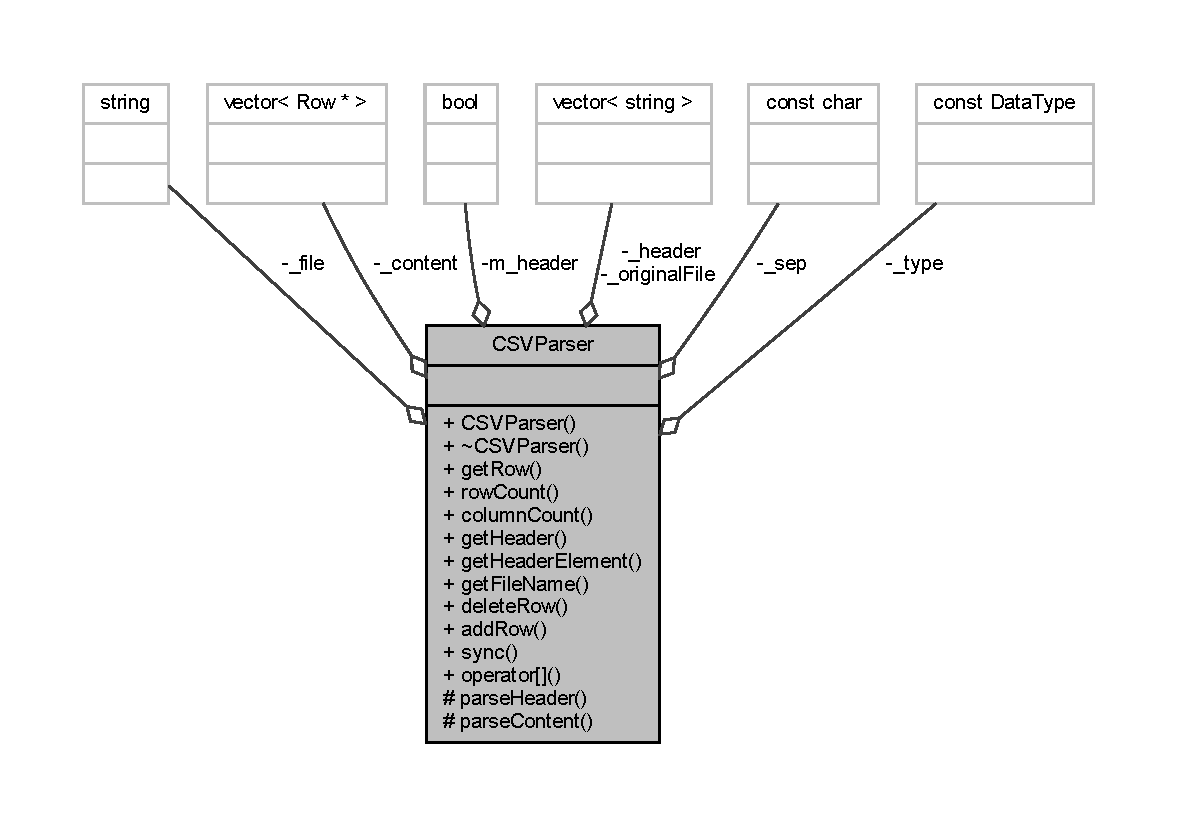
\includegraphics[width=350pt]{class_c_s_v_parser__coll__graph}
\end{center}
\end{figure}
\doxysubsection*{Public Member Functions}
\begin{DoxyCompactItemize}
\item 
\mbox{\hyperlink{class_c_s_v_parser_aba4d9ee88285f39766e7cc810f46d9d9}{C\+S\+V\+Parser}} (const string \&data, const \mbox{\hyperlink{_c_s_vparser_8hpp_ad8ed01ff3ff33333d8e19db4d2818bb6}{Data\+Type}} \&type=\mbox{\hyperlink{_c_s_vparser_8hpp_ad8ed01ff3ff33333d8e19db4d2818bb6a99e2aefa5a03705fd10b8b72e081349f}{e\+F\+I\+LE}}, char sep=\textquotesingle{},\textquotesingle{}, bool has\+Header=true)
\item 
\mbox{\hyperlink{class_c_s_v_parser_a43f06e2e24a260b80e83821c70f91f56}{$\sim$\+C\+S\+V\+Parser}} (void)
\item 
\mbox{\hyperlink{class_row}{Row}} \& \mbox{\hyperlink{class_c_s_v_parser_a93789f318f0abd972860c507b89d4587}{get\+Row}} (unsigned int row) const
\item 
unsigned int \mbox{\hyperlink{class_c_s_v_parser_ab7596d8458539a585908d41638672f4c}{row\+Count}} (void) const
\item 
unsigned int \mbox{\hyperlink{class_c_s_v_parser_a1e30268d574a0c1911de002a893d7a7e}{column\+Count}} (void) const
\item 
vector$<$ string $>$ \mbox{\hyperlink{class_c_s_v_parser_a95b7d4b188facfec7ebab65413f0130b}{get\+Header}} (void) const
\item 
const string \mbox{\hyperlink{class_c_s_v_parser_ad58dc7b467216ecb75f3bea681af3051}{get\+Header\+Element}} (unsigned int pos) const
\item 
const string \& \mbox{\hyperlink{class_c_s_v_parser_ad9a559d1c8de2a7d88a18170c9e11b80}{get\+File\+Name}} (void) const
\item 
bool \mbox{\hyperlink{class_c_s_v_parser_a1bc14d9edecb802c19ad25bd5cab23b3}{delete\+Row}} (unsigned int row)
\item 
bool \mbox{\hyperlink{class_c_s_v_parser_a7e742c5123efa0a49d576776f8832ddb}{add\+Row}} (unsigned int pos, const vector$<$ string $>$ \&r)
\item 
void \mbox{\hyperlink{class_c_s_v_parser_aa0b2494094eb2ce657787ae830b3cc52}{sync}} (void) const
\item 
\mbox{\hyperlink{class_row}{Row}} \& \mbox{\hyperlink{class_c_s_v_parser_a7d3d0c3f994b825aaba25625f0b01612}{operator\mbox{[}$\,$\mbox{]}}} (unsigned int row) const
\end{DoxyCompactItemize}
\doxysubsection*{Protected Member Functions}
\begin{DoxyCompactItemize}
\item 
void \mbox{\hyperlink{class_c_s_v_parser_a8b556e47ecfea188d4c6c630616f5667}{parse\+Header}} (void)
\item 
void \mbox{\hyperlink{class_c_s_v_parser_aa403f7d8238903aa0e046a9a091ab968}{parse\+Content}} (void)
\end{DoxyCompactItemize}
\doxysubsection*{Private Attributes}
\begin{DoxyCompactItemize}
\item 
string \mbox{\hyperlink{class_c_s_v_parser_a1db17c9285f8fdcaed2499747582e4a9}{\+\_\+file}}
\item 
const \mbox{\hyperlink{_c_s_vparser_8hpp_ad8ed01ff3ff33333d8e19db4d2818bb6}{Data\+Type}} \mbox{\hyperlink{class_c_s_v_parser_a27cff8e618160b2685f1e05b8a7da9cf}{\+\_\+type}}
\item 
const char \mbox{\hyperlink{class_c_s_v_parser_a9d778da8bd668d2393d4402ce7eae9cd}{\+\_\+sep}}
\item 
vector$<$ string $>$ \mbox{\hyperlink{class_c_s_v_parser_afa0c154dd897b5ddcbf8364a9df28eeb}{\+\_\+original\+File}}
\item 
vector$<$ string $>$ \mbox{\hyperlink{class_c_s_v_parser_a9b35b0a143febb8fb388769417fa0777}{\+\_\+header}}
\item 
vector$<$ \mbox{\hyperlink{class_row}{Row}} $\ast$ $>$ \mbox{\hyperlink{class_c_s_v_parser_adff6872f7e93cbc10797bac6173671d4}{\+\_\+content}}
\item 
bool \mbox{\hyperlink{class_c_s_v_parser_a4dcb7bb113b65d0abf816dd899395545}{m\+\_\+header}}
\end{DoxyCompactItemize}


\doxysubsection{Detailed Description}
This class is used to read and parse a csv file or to write some values as a csv file. 

\doxysubsection{Constructor \& Destructor Documentation}
\mbox{\Hypertarget{class_c_s_v_parser_aba4d9ee88285f39766e7cc810f46d9d9}\label{class_c_s_v_parser_aba4d9ee88285f39766e7cc810f46d9d9}} 
\index{CSVParser@{CSVParser}!CSVParser@{CSVParser}}
\index{CSVParser@{CSVParser}!CSVParser@{CSVParser}}
\doxysubsubsection{\texorpdfstring{CSVParser()}{CSVParser()}}
{\footnotesize\ttfamily C\+S\+V\+Parser\+::\+C\+S\+V\+Parser (\begin{DoxyParamCaption}\item[{const string \&}]{data,  }\item[{const \mbox{\hyperlink{_c_s_vparser_8hpp_ad8ed01ff3ff33333d8e19db4d2818bb6}{Data\+Type}} \&}]{type = {\ttfamily \mbox{\hyperlink{_c_s_vparser_8hpp_ad8ed01ff3ff33333d8e19db4d2818bb6a99e2aefa5a03705fd10b8b72e081349f}{e\+F\+I\+LE}}},  }\item[{char}]{sep = {\ttfamily \textquotesingle{},\textquotesingle{}},  }\item[{bool}]{has\+Header = {\ttfamily true} }\end{DoxyParamCaption})}

Constructor of the class. It need the name of the csv file, the file type, the separator and a boolean that indicates if the file has header or not. 
\begin{DoxyParams}{Parameters}
{\em data} & the name of the file \\
\hline
{\em type} & the file type\+: could be e\+F\+I\+LE for normal text files or e\+P\+U\+RE if the input is a string \\
\hline
{\em sep} & the separator of the individula values in a line of the csv file \\
\hline
{\em has\+Header} & true means that the csv file has a header line, false that it doesn\textquotesingle{}t have a header \\
\hline
\end{DoxyParams}
\mbox{\Hypertarget{class_c_s_v_parser_a43f06e2e24a260b80e83821c70f91f56}\label{class_c_s_v_parser_a43f06e2e24a260b80e83821c70f91f56}} 
\index{CSVParser@{CSVParser}!````~CSVParser@{$\sim$CSVParser}}
\index{````~CSVParser@{$\sim$CSVParser}!CSVParser@{CSVParser}}
\doxysubsubsection{\texorpdfstring{$\sim$CSVParser()}{~CSVParser()}}
{\footnotesize\ttfamily C\+S\+V\+Parser\+::$\sim$\+C\+S\+V\+Parser (\begin{DoxyParamCaption}\item[{void}]{ }\end{DoxyParamCaption})}

Destructor 

\doxysubsection{Member Function Documentation}
\mbox{\Hypertarget{class_c_s_v_parser_a7e742c5123efa0a49d576776f8832ddb}\label{class_c_s_v_parser_a7e742c5123efa0a49d576776f8832ddb}} 
\index{CSVParser@{CSVParser}!addRow@{addRow}}
\index{addRow@{addRow}!CSVParser@{CSVParser}}
\doxysubsubsection{\texorpdfstring{addRow()}{addRow()}}
{\footnotesize\ttfamily bool C\+S\+V\+Parser\+::add\+Row (\begin{DoxyParamCaption}\item[{unsigned int}]{pos,  }\item[{const vector$<$ string $>$ \&}]{r }\end{DoxyParamCaption})}

Inserts a \mbox{\hyperlink{class_row}{Row}} object at a given position 
\begin{DoxyParams}{Parameters}
{\em pos} & the position where we want to insert the \mbox{\hyperlink{class_row}{Row}} object \\
\hline
{\em r} & a vector containing the values in the \mbox{\hyperlink{class_row}{Row}}. \\
\hline
\end{DoxyParams}
\begin{DoxyReturn}{Returns}
true if the insertion is successful, false otherwise (i.\+e. the pos parameter is outside the limits of the container that stores the Rows of the csv file. 
\end{DoxyReturn}
\mbox{\Hypertarget{class_c_s_v_parser_a1e30268d574a0c1911de002a893d7a7e}\label{class_c_s_v_parser_a1e30268d574a0c1911de002a893d7a7e}} 
\index{CSVParser@{CSVParser}!columnCount@{columnCount}}
\index{columnCount@{columnCount}!CSVParser@{CSVParser}}
\doxysubsubsection{\texorpdfstring{columnCount()}{columnCount()}}
{\footnotesize\ttfamily unsigned int C\+S\+V\+Parser\+::column\+Count (\begin{DoxyParamCaption}\item[{void}]{ }\end{DoxyParamCaption}) const}

Returns the number of the columns of the csv file. \begin{DoxyReturn}{Returns}
the number of the columns of the csv file. 
\end{DoxyReturn}
\mbox{\Hypertarget{class_c_s_v_parser_a1bc14d9edecb802c19ad25bd5cab23b3}\label{class_c_s_v_parser_a1bc14d9edecb802c19ad25bd5cab23b3}} 
\index{CSVParser@{CSVParser}!deleteRow@{deleteRow}}
\index{deleteRow@{deleteRow}!CSVParser@{CSVParser}}
\doxysubsubsection{\texorpdfstring{deleteRow()}{deleteRow()}}
{\footnotesize\ttfamily bool C\+S\+V\+Parser\+::delete\+Row (\begin{DoxyParamCaption}\item[{unsigned int}]{row }\end{DoxyParamCaption})}

Removes a row specified by its number 
\begin{DoxyParams}{Parameters}
{\em row} & the number of the row to be deleted \\
\hline
\end{DoxyParams}
\begin{DoxyReturn}{Returns}
true if the removal succeeded, false otherwise 
\end{DoxyReturn}
\mbox{\Hypertarget{class_c_s_v_parser_ad9a559d1c8de2a7d88a18170c9e11b80}\label{class_c_s_v_parser_ad9a559d1c8de2a7d88a18170c9e11b80}} 
\index{CSVParser@{CSVParser}!getFileName@{getFileName}}
\index{getFileName@{getFileName}!CSVParser@{CSVParser}}
\doxysubsubsection{\texorpdfstring{getFileName()}{getFileName()}}
{\footnotesize\ttfamily const string\& C\+S\+V\+Parser\+::get\+File\+Name (\begin{DoxyParamCaption}\item[{void}]{ }\end{DoxyParamCaption}) const}

Returns the name of the csv file \begin{DoxyReturn}{Returns}
the name of the csv file 
\end{DoxyReturn}
\mbox{\Hypertarget{class_c_s_v_parser_a95b7d4b188facfec7ebab65413f0130b}\label{class_c_s_v_parser_a95b7d4b188facfec7ebab65413f0130b}} 
\index{CSVParser@{CSVParser}!getHeader@{getHeader}}
\index{getHeader@{getHeader}!CSVParser@{CSVParser}}
\doxysubsubsection{\texorpdfstring{getHeader()}{getHeader()}}
{\footnotesize\ttfamily vector$<$string$>$ C\+S\+V\+Parser\+::get\+Header (\begin{DoxyParamCaption}\item[{void}]{ }\end{DoxyParamCaption}) const}

Returns a vector containing the names of the columns as they are specified in the header line of the csv file. \begin{DoxyReturn}{Returns}
a vector containing the names of the columns as they are specified in the header line of the csv file. 
\end{DoxyReturn}
\mbox{\Hypertarget{class_c_s_v_parser_ad58dc7b467216ecb75f3bea681af3051}\label{class_c_s_v_parser_ad58dc7b467216ecb75f3bea681af3051}} 
\index{CSVParser@{CSVParser}!getHeaderElement@{getHeaderElement}}
\index{getHeaderElement@{getHeaderElement}!CSVParser@{CSVParser}}
\doxysubsubsection{\texorpdfstring{getHeaderElement()}{getHeaderElement()}}
{\footnotesize\ttfamily const string C\+S\+V\+Parser\+::get\+Header\+Element (\begin{DoxyParamCaption}\item[{unsigned int}]{pos }\end{DoxyParamCaption}) const}

Returns the name of a specific column given by its position in the header line 
\begin{DoxyParams}{Parameters}
{\em pos} & the number of the column \\
\hline
\end{DoxyParams}
\begin{DoxyReturn}{Returns}
the name of a specific column given by its position in the header line 
\end{DoxyReturn}
\mbox{\Hypertarget{class_c_s_v_parser_a93789f318f0abd972860c507b89d4587}\label{class_c_s_v_parser_a93789f318f0abd972860c507b89d4587}} 
\index{CSVParser@{CSVParser}!getRow@{getRow}}
\index{getRow@{getRow}!CSVParser@{CSVParser}}
\doxysubsubsection{\texorpdfstring{getRow()}{getRow()}}
{\footnotesize\ttfamily \mbox{\hyperlink{class_row}{Row}}\& C\+S\+V\+Parser\+::get\+Row (\begin{DoxyParamCaption}\item[{unsigned int}]{row }\end{DoxyParamCaption}) const}

Returns a \mbox{\hyperlink{class_row}{Row}} object specified by its number in the file 
\begin{DoxyParams}{Parameters}
{\em row} & the number of the line that was used to build the \mbox{\hyperlink{class_row}{Row}} object \\
\hline
\end{DoxyParams}
\begin{DoxyReturn}{Returns}
a \mbox{\hyperlink{class_row}{Row}} object specified by its number in the file 
\end{DoxyReturn}
\mbox{\Hypertarget{class_c_s_v_parser_a7d3d0c3f994b825aaba25625f0b01612}\label{class_c_s_v_parser_a7d3d0c3f994b825aaba25625f0b01612}} 
\index{CSVParser@{CSVParser}!operator\mbox{[}\mbox{]}@{operator[]}}
\index{operator\mbox{[}\mbox{]}@{operator[]}!CSVParser@{CSVParser}}
\doxysubsubsection{\texorpdfstring{operator[]()}{operator[]()}}
{\footnotesize\ttfamily \mbox{\hyperlink{class_row}{Row}}\& C\+S\+V\+Parser\+::operator\mbox{[}$\,$\mbox{]} (\begin{DoxyParamCaption}\item[{unsigned int}]{row }\end{DoxyParamCaption}) const}

Overloaded operator 
\begin{DoxyParams}{Parameters}
{\em row} & the number of the row to be retrieved \\
\hline
\end{DoxyParams}
\begin{DoxyReturn}{Returns}
the \mbox{\hyperlink{class_row}{Row}} object at the position specified by row 
\end{DoxyReturn}
\mbox{\Hypertarget{class_c_s_v_parser_aa403f7d8238903aa0e046a9a091ab968}\label{class_c_s_v_parser_aa403f7d8238903aa0e046a9a091ab968}} 
\index{CSVParser@{CSVParser}!parseContent@{parseContent}}
\index{parseContent@{parseContent}!CSVParser@{CSVParser}}
\doxysubsubsection{\texorpdfstring{parseContent()}{parseContent()}}
{\footnotesize\ttfamily void C\+S\+V\+Parser\+::parse\+Content (\begin{DoxyParamCaption}\item[{void}]{ }\end{DoxyParamCaption})\hspace{0.3cm}{\ttfamily [protected]}}

\mbox{\Hypertarget{class_c_s_v_parser_a8b556e47ecfea188d4c6c630616f5667}\label{class_c_s_v_parser_a8b556e47ecfea188d4c6c630616f5667}} 
\index{CSVParser@{CSVParser}!parseHeader@{parseHeader}}
\index{parseHeader@{parseHeader}!CSVParser@{CSVParser}}
\doxysubsubsection{\texorpdfstring{parseHeader()}{parseHeader()}}
{\footnotesize\ttfamily void C\+S\+V\+Parser\+::parse\+Header (\begin{DoxyParamCaption}\item[{void}]{ }\end{DoxyParamCaption})\hspace{0.3cm}{\ttfamily [protected]}}

\mbox{\Hypertarget{class_c_s_v_parser_ab7596d8458539a585908d41638672f4c}\label{class_c_s_v_parser_ab7596d8458539a585908d41638672f4c}} 
\index{CSVParser@{CSVParser}!rowCount@{rowCount}}
\index{rowCount@{rowCount}!CSVParser@{CSVParser}}
\doxysubsubsection{\texorpdfstring{rowCount()}{rowCount()}}
{\footnotesize\ttfamily unsigned int C\+S\+V\+Parser\+::row\+Count (\begin{DoxyParamCaption}\item[{void}]{ }\end{DoxyParamCaption}) const}

Returns the number of lines in the csv file without counting the header line, if it exists \begin{DoxyReturn}{Returns}
the number of lines in the csv file without counting the header line, if it exists 
\end{DoxyReturn}
\mbox{\Hypertarget{class_c_s_v_parser_aa0b2494094eb2ce657787ae830b3cc52}\label{class_c_s_v_parser_aa0b2494094eb2ce657787ae830b3cc52}} 
\index{CSVParser@{CSVParser}!sync@{sync}}
\index{sync@{sync}!CSVParser@{CSVParser}}
\doxysubsubsection{\texorpdfstring{sync()}{sync()}}
{\footnotesize\ttfamily void C\+S\+V\+Parser\+::sync (\begin{DoxyParamCaption}\item[{void}]{ }\end{DoxyParamCaption}) const}

Flushes the content to a file on disk and then closes the file. 

\doxysubsection{Member Data Documentation}
\mbox{\Hypertarget{class_c_s_v_parser_adff6872f7e93cbc10797bac6173671d4}\label{class_c_s_v_parser_adff6872f7e93cbc10797bac6173671d4}} 
\index{CSVParser@{CSVParser}!\_content@{\_content}}
\index{\_content@{\_content}!CSVParser@{CSVParser}}
\doxysubsubsection{\texorpdfstring{\_content}{\_content}}
{\footnotesize\ttfamily vector$<$\mbox{\hyperlink{class_row}{Row}} $\ast$$>$ C\+S\+V\+Parser\+::\+\_\+content\hspace{0.3cm}{\ttfamily [private]}}

\mbox{\Hypertarget{class_c_s_v_parser_a1db17c9285f8fdcaed2499747582e4a9}\label{class_c_s_v_parser_a1db17c9285f8fdcaed2499747582e4a9}} 
\index{CSVParser@{CSVParser}!\_file@{\_file}}
\index{\_file@{\_file}!CSVParser@{CSVParser}}
\doxysubsubsection{\texorpdfstring{\_file}{\_file}}
{\footnotesize\ttfamily string C\+S\+V\+Parser\+::\+\_\+file\hspace{0.3cm}{\ttfamily [private]}}

\mbox{\Hypertarget{class_c_s_v_parser_a9b35b0a143febb8fb388769417fa0777}\label{class_c_s_v_parser_a9b35b0a143febb8fb388769417fa0777}} 
\index{CSVParser@{CSVParser}!\_header@{\_header}}
\index{\_header@{\_header}!CSVParser@{CSVParser}}
\doxysubsubsection{\texorpdfstring{\_header}{\_header}}
{\footnotesize\ttfamily vector$<$string$>$ C\+S\+V\+Parser\+::\+\_\+header\hspace{0.3cm}{\ttfamily [private]}}

\mbox{\Hypertarget{class_c_s_v_parser_afa0c154dd897b5ddcbf8364a9df28eeb}\label{class_c_s_v_parser_afa0c154dd897b5ddcbf8364a9df28eeb}} 
\index{CSVParser@{CSVParser}!\_originalFile@{\_originalFile}}
\index{\_originalFile@{\_originalFile}!CSVParser@{CSVParser}}
\doxysubsubsection{\texorpdfstring{\_originalFile}{\_originalFile}}
{\footnotesize\ttfamily vector$<$string$>$ C\+S\+V\+Parser\+::\+\_\+original\+File\hspace{0.3cm}{\ttfamily [private]}}

\mbox{\Hypertarget{class_c_s_v_parser_a9d778da8bd668d2393d4402ce7eae9cd}\label{class_c_s_v_parser_a9d778da8bd668d2393d4402ce7eae9cd}} 
\index{CSVParser@{CSVParser}!\_sep@{\_sep}}
\index{\_sep@{\_sep}!CSVParser@{CSVParser}}
\doxysubsubsection{\texorpdfstring{\_sep}{\_sep}}
{\footnotesize\ttfamily const char C\+S\+V\+Parser\+::\+\_\+sep\hspace{0.3cm}{\ttfamily [private]}}

\mbox{\Hypertarget{class_c_s_v_parser_a27cff8e618160b2685f1e05b8a7da9cf}\label{class_c_s_v_parser_a27cff8e618160b2685f1e05b8a7da9cf}} 
\index{CSVParser@{CSVParser}!\_type@{\_type}}
\index{\_type@{\_type}!CSVParser@{CSVParser}}
\doxysubsubsection{\texorpdfstring{\_type}{\_type}}
{\footnotesize\ttfamily const \mbox{\hyperlink{_c_s_vparser_8hpp_ad8ed01ff3ff33333d8e19db4d2818bb6}{Data\+Type}} C\+S\+V\+Parser\+::\+\_\+type\hspace{0.3cm}{\ttfamily [private]}}

\mbox{\Hypertarget{class_c_s_v_parser_a4dcb7bb113b65d0abf816dd899395545}\label{class_c_s_v_parser_a4dcb7bb113b65d0abf816dd899395545}} 
\index{CSVParser@{CSVParser}!m\_header@{m\_header}}
\index{m\_header@{m\_header}!CSVParser@{CSVParser}}
\doxysubsubsection{\texorpdfstring{m\_header}{m\_header}}
{\footnotesize\ttfamily bool C\+S\+V\+Parser\+::m\+\_\+header\hspace{0.3cm}{\ttfamily [private]}}



The documentation for this class was generated from the following file\+:\begin{DoxyCompactItemize}
\item 
include/\mbox{\hyperlink{_c_s_vparser_8hpp}{C\+S\+Vparser.\+hpp}}\end{DoxyCompactItemize}

\hypertarget{class_displace}{}\doxysection{Displace Class Reference}
\label{class_displace}\index{Displace@{Displace}}


{\ttfamily \#include $<$Displace.\+h$>$}



Inheritance diagram for Displace\+:\nopagebreak
\begin{figure}[H]
\begin{center}
\leavevmode
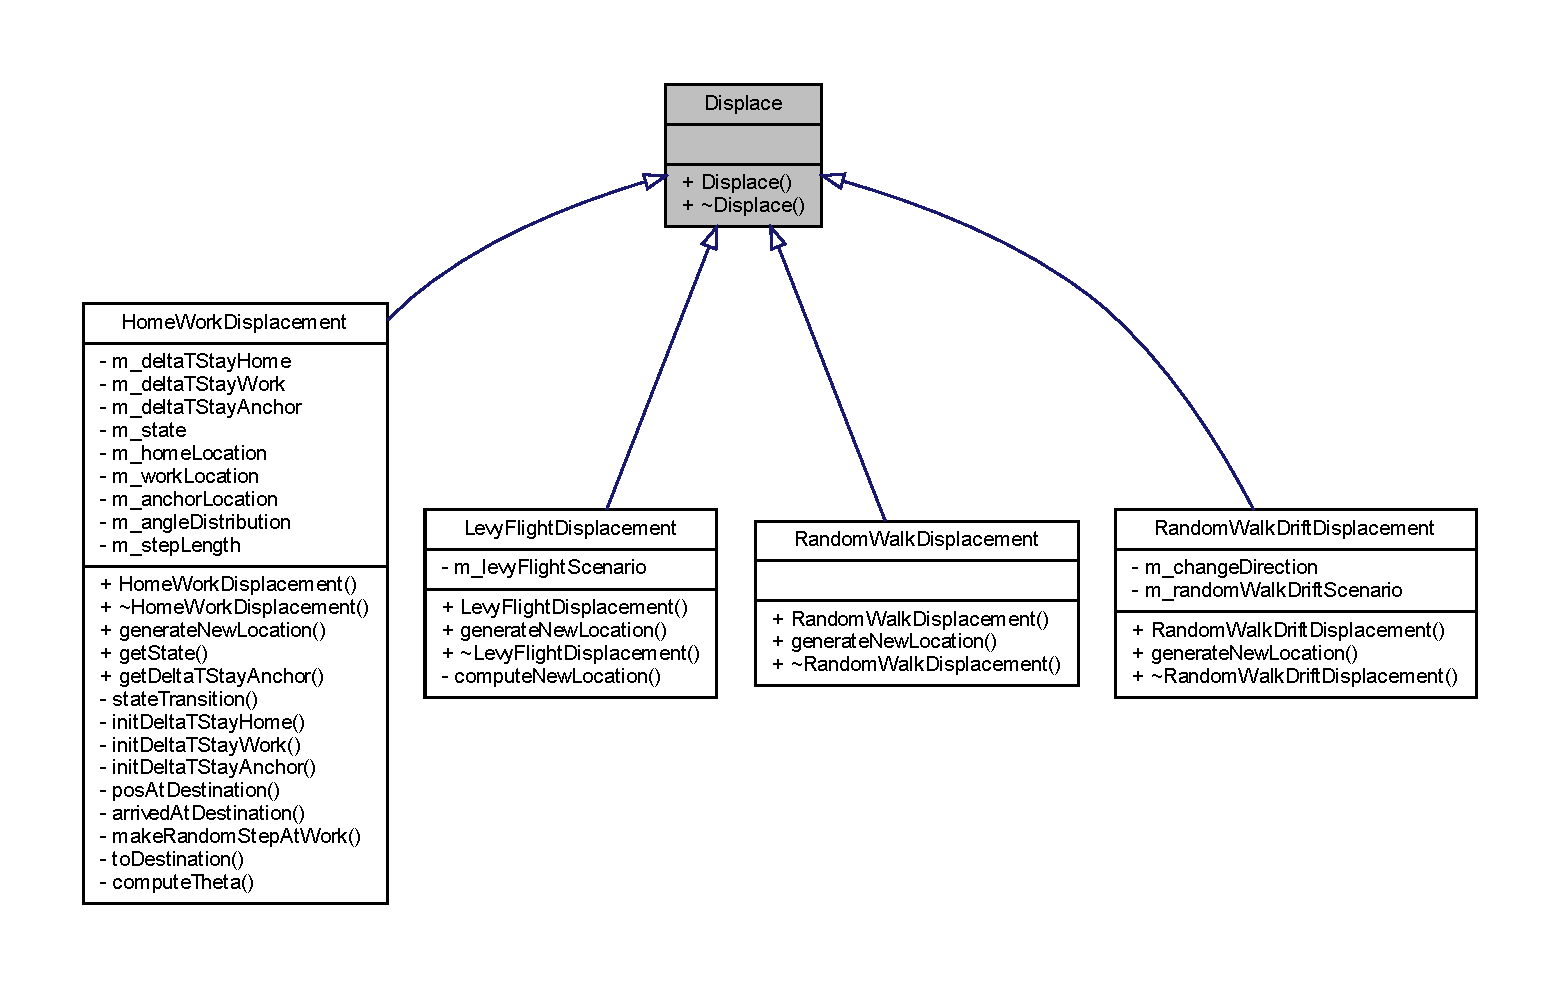
\includegraphics[width=350pt]{class_displace__inherit__graph}
\end{center}
\end{figure}


Collaboration diagram for Displace\+:\nopagebreak
\begin{figure}[H]
\begin{center}
\leavevmode
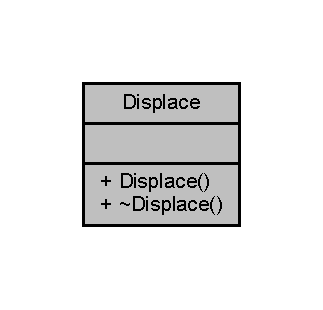
\includegraphics[width=155pt]{class_displace__coll__graph}
\end{center}
\end{figure}
\doxysubsection*{Public Member Functions}
\begin{DoxyCompactItemize}
\item 
\mbox{\hyperlink{class_displace_a7a5e8789c200aac40ce08272e5488af0}{Displace}} (\mbox{\hyperlink{class_simulation_configuration}{Simulation\+Configuration}} $\ast$simconfig, double speed)
\item 
virtual \mbox{\hyperlink{class_displace_a8d3969cda060cd7419e337a3f232be97}{$\sim$\+Displace}} ()
\end{DoxyCompactItemize}


\doxysubsection{Detailed Description}
This class implements a Strategy design pattern. It acts as an interface to different displacement algorithms. 

\doxysubsection{Constructor \& Destructor Documentation}
\mbox{\Hypertarget{class_displace_a7a5e8789c200aac40ce08272e5488af0}\label{class_displace_a7a5e8789c200aac40ce08272e5488af0}} 
\index{Displace@{Displace}!Displace@{Displace}}
\index{Displace@{Displace}!Displace@{Displace}}
\doxysubsubsection{\texorpdfstring{Displace()}{Displace()}}
{\footnotesize\ttfamily Displace\+::\+Displace (\begin{DoxyParamCaption}\item[{\mbox{\hyperlink{class_simulation_configuration}{Simulation\+Configuration}} $\ast$}]{simconfig,  }\item[{double}]{speed }\end{DoxyParamCaption})}

Constructor of the class. Initializes members. 
\begin{DoxyParams}{Parameters}
{\em speed} & the speed of displacement. \\
\hline
\end{DoxyParams}
\mbox{\Hypertarget{class_displace_a8d3969cda060cd7419e337a3f232be97}\label{class_displace_a8d3969cda060cd7419e337a3f232be97}} 
\index{Displace@{Displace}!````~Displace@{$\sim$Displace}}
\index{````~Displace@{$\sim$Displace}!Displace@{Displace}}
\doxysubsubsection{\texorpdfstring{$\sim$Displace()}{~Displace()}}
{\footnotesize\ttfamily virtual Displace\+::$\sim$\+Displace (\begin{DoxyParamCaption}{ }\end{DoxyParamCaption})\hspace{0.3cm}{\ttfamily [virtual]}}

Default destructor. 

The documentation for this class was generated from the following file\+:\begin{DoxyCompactItemize}
\item 
include/\mbox{\hyperlink{_displace_8h}{Displace.\+h}}\end{DoxyCompactItemize}

\hypertarget{class_distribution}{}\doxysection{Distribution Class Reference}
\label{class_distribution}\index{Distribution@{Distribution}}


{\ttfamily \#include $<$Distribution.\+h$>$}



Collaboration diagram for Distribution\+:\nopagebreak
\begin{figure}[H]
\begin{center}
\leavevmode
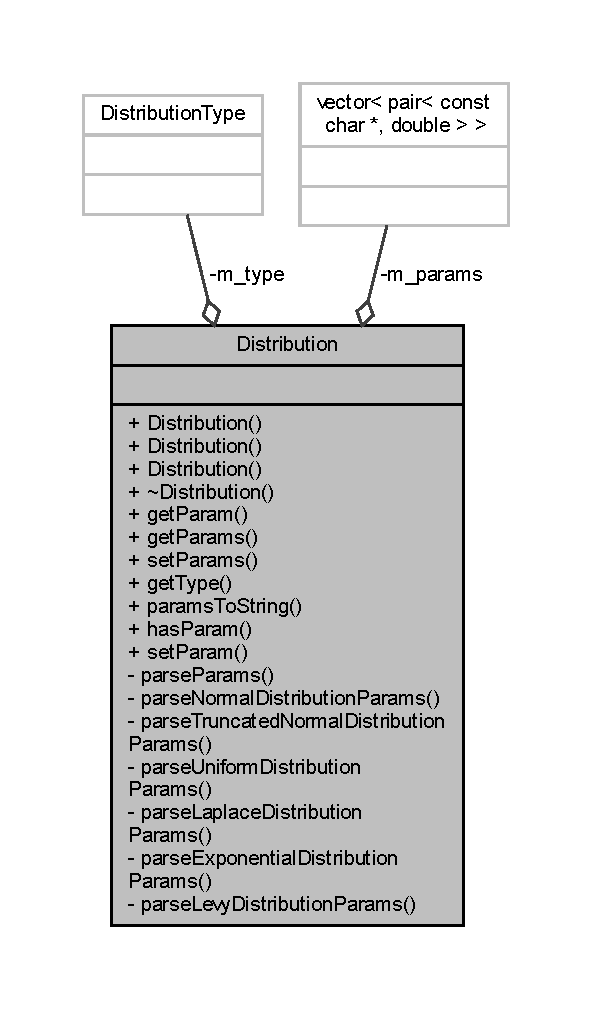
\includegraphics[width=284pt]{class_distribution__coll__graph}
\end{center}
\end{figure}
\doxysubsection*{Public Member Functions}
\begin{DoxyCompactItemize}
\item 
\mbox{\hyperlink{class_distribution_a8a0b2be74f8a370c4fee8a34de41642a}{Distribution}} ()=delete
\item 
\mbox{\hyperlink{class_distribution_a87a40f253be841f7b90fb3f0b3a76e79}{Distribution}} (\mbox{\hyperlink{_distribution_type_8h_a379a030cc5c116910d8ac63ada868a62}{Distribution\+Type}} type, vector$<$ pair$<$ const char $\ast$, double $>$$>$ params)
\item 
\mbox{\hyperlink{class_distribution_add160cb1d3377d93612d439841546c57}{Distribution}} (\mbox{\hyperlink{_distribution_type_8h_a379a030cc5c116910d8ac63ada868a62}{Distribution\+Type}} type, X\+M\+L\+Element $\ast$element)
\item 
virtual \mbox{\hyperlink{class_distribution_a0b585e4cc1a10cf3628e27e8a81c9c72}{$\sim$\+Distribution}} ()
\item 
double \mbox{\hyperlink{class_distribution_ab77dc824578e18acfb0de381ee612bb9}{get\+Param}} (const char $\ast$name)
\item 
vector$<$ pair$<$ const char $\ast$, double $>$ $>$ \& \mbox{\hyperlink{class_distribution_ac2991bcf0f9f99ebad6ba48e490b2da6}{get\+Params}} ()
\item 
void \mbox{\hyperlink{class_distribution_a51420bfbe3ca31af8d9bfaa6a5df6e34}{set\+Params}} (vector$<$ pair$<$ const char $\ast$, double $>$$>$ params)
\item 
\mbox{\hyperlink{_distribution_type_8h_a379a030cc5c116910d8ac63ada868a62}{Distribution\+Type}} \mbox{\hyperlink{class_distribution_a66e558c60a81b732ce174db8c873b09e}{get\+Type}} ()
\item 
string \mbox{\hyperlink{class_distribution_a0f76f314a1f0fbd6024b0ee74022d7b4}{params\+To\+String}} ()
\item 
bool \mbox{\hyperlink{class_distribution_aed03103bd77adc278e6e34824f4390a2}{has\+Param}} (const char $\ast$name) const
\item 
void \mbox{\hyperlink{class_distribution_a8c76d815d553dd75e15b2d249531085d}{set\+Param}} (const char $\ast$name, double value)
\end{DoxyCompactItemize}
\doxysubsection*{Private Member Functions}
\begin{DoxyCompactItemize}
\item 
void \mbox{\hyperlink{class_distribution_aa3ddf2f8e4edd64062e4378c07d9b1c1}{parse\+Params}} (\mbox{\hyperlink{_distribution_type_8h_a379a030cc5c116910d8ac63ada868a62}{Distribution\+Type}} type, X\+M\+L\+Element $\ast$element)
\item 
void \mbox{\hyperlink{class_distribution_a1837b0276c7f5dc43a458fb6f2178166}{parse\+Normal\+Distribution\+Params}} (X\+M\+L\+Element $\ast$el)
\item 
void \mbox{\hyperlink{class_distribution_a899eae918b09d795cd31e46aac276241}{parse\+Truncated\+Normal\+Distribution\+Params}} (X\+M\+L\+Element $\ast$el)
\item 
void \mbox{\hyperlink{class_distribution_a5f0d5da3398ea484bdaed2918d1b419e}{parse\+Uniform\+Distribution\+Params}} (X\+M\+L\+Element $\ast$el)
\item 
void \mbox{\hyperlink{class_distribution_ad177ead4f076c7aebd5703ed24a09d1e}{parse\+Laplace\+Distribution\+Params}} (X\+M\+L\+Element $\ast$el)
\item 
void \mbox{\hyperlink{class_distribution_a7c60f66779b215693a8bc072013d784f}{parse\+Exponential\+Distribution\+Params}} (X\+M\+L\+Element $\ast$el)
\item 
void \mbox{\hyperlink{class_distribution_a446d54f3ca7377f4046687b101267534}{parse\+Levy\+Distribution\+Params}} (X\+M\+L\+Element $\ast$el)
\end{DoxyCompactItemize}
\doxysubsection*{Private Attributes}
\begin{DoxyCompactItemize}
\item 
\mbox{\hyperlink{_distribution_type_8h_a379a030cc5c116910d8ac63ada868a62}{Distribution\+Type}} \mbox{\hyperlink{class_distribution_aaabe7a3c22bf6c0a0d24a80454764133}{m\+\_\+type}}
\item 
vector$<$ pair$<$ const char $\ast$, double $>$ $>$ \mbox{\hyperlink{class_distribution_a29c3699182136f52c91abd7d42efa823}{m\+\_\+params}}
\end{DoxyCompactItemize}


\doxysubsection{Constructor \& Destructor Documentation}
\mbox{\Hypertarget{class_distribution_a8a0b2be74f8a370c4fee8a34de41642a}\label{class_distribution_a8a0b2be74f8a370c4fee8a34de41642a}} 
\index{Distribution@{Distribution}!Distribution@{Distribution}}
\index{Distribution@{Distribution}!Distribution@{Distribution}}
\doxysubsubsection{\texorpdfstring{Distribution()}{Distribution()}\hspace{0.1cm}{\footnotesize\ttfamily [1/3]}}
{\footnotesize\ttfamily Distribution\+::\+Distribution (\begin{DoxyParamCaption}{ }\end{DoxyParamCaption})\hspace{0.3cm}{\ttfamily [delete]}}

\mbox{\Hypertarget{class_distribution_a87a40f253be841f7b90fb3f0b3a76e79}\label{class_distribution_a87a40f253be841f7b90fb3f0b3a76e79}} 
\index{Distribution@{Distribution}!Distribution@{Distribution}}
\index{Distribution@{Distribution}!Distribution@{Distribution}}
\doxysubsubsection{\texorpdfstring{Distribution()}{Distribution()}\hspace{0.1cm}{\footnotesize\ttfamily [2/3]}}
{\footnotesize\ttfamily Distribution\+::\+Distribution (\begin{DoxyParamCaption}\item[{\mbox{\hyperlink{_distribution_type_8h_a379a030cc5c116910d8ac63ada868a62}{Distribution\+Type}}}]{type,  }\item[{vector$<$ pair$<$ const char $\ast$, double $>$$>$}]{params }\end{DoxyParamCaption})}

\mbox{\Hypertarget{class_distribution_add160cb1d3377d93612d439841546c57}\label{class_distribution_add160cb1d3377d93612d439841546c57}} 
\index{Distribution@{Distribution}!Distribution@{Distribution}}
\index{Distribution@{Distribution}!Distribution@{Distribution}}
\doxysubsubsection{\texorpdfstring{Distribution()}{Distribution()}\hspace{0.1cm}{\footnotesize\ttfamily [3/3]}}
{\footnotesize\ttfamily Distribution\+::\+Distribution (\begin{DoxyParamCaption}\item[{\mbox{\hyperlink{_distribution_type_8h_a379a030cc5c116910d8ac63ada868a62}{Distribution\+Type}}}]{type,  }\item[{X\+M\+L\+Element $\ast$}]{element }\end{DoxyParamCaption})}

\mbox{\Hypertarget{class_distribution_a0b585e4cc1a10cf3628e27e8a81c9c72}\label{class_distribution_a0b585e4cc1a10cf3628e27e8a81c9c72}} 
\index{Distribution@{Distribution}!````~Distribution@{$\sim$Distribution}}
\index{````~Distribution@{$\sim$Distribution}!Distribution@{Distribution}}
\doxysubsubsection{\texorpdfstring{$\sim$Distribution()}{~Distribution()}}
{\footnotesize\ttfamily virtual Distribution\+::$\sim$\+Distribution (\begin{DoxyParamCaption}{ }\end{DoxyParamCaption})\hspace{0.3cm}{\ttfamily [virtual]}}



\doxysubsection{Member Function Documentation}
\mbox{\Hypertarget{class_distribution_ab77dc824578e18acfb0de381ee612bb9}\label{class_distribution_ab77dc824578e18acfb0de381ee612bb9}} 
\index{Distribution@{Distribution}!getParam@{getParam}}
\index{getParam@{getParam}!Distribution@{Distribution}}
\doxysubsubsection{\texorpdfstring{getParam()}{getParam()}}
{\footnotesize\ttfamily double Distribution\+::get\+Param (\begin{DoxyParamCaption}\item[{const char $\ast$}]{name }\end{DoxyParamCaption})}

\mbox{\Hypertarget{class_distribution_ac2991bcf0f9f99ebad6ba48e490b2da6}\label{class_distribution_ac2991bcf0f9f99ebad6ba48e490b2da6}} 
\index{Distribution@{Distribution}!getParams@{getParams}}
\index{getParams@{getParams}!Distribution@{Distribution}}
\doxysubsubsection{\texorpdfstring{getParams()}{getParams()}}
{\footnotesize\ttfamily vector$<$pair$<$const char$\ast$, double$>$ $>$\& Distribution\+::get\+Params (\begin{DoxyParamCaption}{ }\end{DoxyParamCaption})}

\mbox{\Hypertarget{class_distribution_a66e558c60a81b732ce174db8c873b09e}\label{class_distribution_a66e558c60a81b732ce174db8c873b09e}} 
\index{Distribution@{Distribution}!getType@{getType}}
\index{getType@{getType}!Distribution@{Distribution}}
\doxysubsubsection{\texorpdfstring{getType()}{getType()}}
{\footnotesize\ttfamily \mbox{\hyperlink{_distribution_type_8h_a379a030cc5c116910d8ac63ada868a62}{Distribution\+Type}} Distribution\+::get\+Type (\begin{DoxyParamCaption}{ }\end{DoxyParamCaption})}

\mbox{\Hypertarget{class_distribution_aed03103bd77adc278e6e34824f4390a2}\label{class_distribution_aed03103bd77adc278e6e34824f4390a2}} 
\index{Distribution@{Distribution}!hasParam@{hasParam}}
\index{hasParam@{hasParam}!Distribution@{Distribution}}
\doxysubsubsection{\texorpdfstring{hasParam()}{hasParam()}}
{\footnotesize\ttfamily bool Distribution\+::has\+Param (\begin{DoxyParamCaption}\item[{const char $\ast$}]{name }\end{DoxyParamCaption}) const}

\mbox{\Hypertarget{class_distribution_a0f76f314a1f0fbd6024b0ee74022d7b4}\label{class_distribution_a0f76f314a1f0fbd6024b0ee74022d7b4}} 
\index{Distribution@{Distribution}!paramsToString@{paramsToString}}
\index{paramsToString@{paramsToString}!Distribution@{Distribution}}
\doxysubsubsection{\texorpdfstring{paramsToString()}{paramsToString()}}
{\footnotesize\ttfamily string Distribution\+::params\+To\+String (\begin{DoxyParamCaption}{ }\end{DoxyParamCaption})}

\mbox{\Hypertarget{class_distribution_a7c60f66779b215693a8bc072013d784f}\label{class_distribution_a7c60f66779b215693a8bc072013d784f}} 
\index{Distribution@{Distribution}!parseExponentialDistributionParams@{parseExponentialDistributionParams}}
\index{parseExponentialDistributionParams@{parseExponentialDistributionParams}!Distribution@{Distribution}}
\doxysubsubsection{\texorpdfstring{parseExponentialDistributionParams()}{parseExponentialDistributionParams()}}
{\footnotesize\ttfamily void Distribution\+::parse\+Exponential\+Distribution\+Params (\begin{DoxyParamCaption}\item[{X\+M\+L\+Element $\ast$}]{el }\end{DoxyParamCaption})\hspace{0.3cm}{\ttfamily [private]}}

\mbox{\Hypertarget{class_distribution_ad177ead4f076c7aebd5703ed24a09d1e}\label{class_distribution_ad177ead4f076c7aebd5703ed24a09d1e}} 
\index{Distribution@{Distribution}!parseLaplaceDistributionParams@{parseLaplaceDistributionParams}}
\index{parseLaplaceDistributionParams@{parseLaplaceDistributionParams}!Distribution@{Distribution}}
\doxysubsubsection{\texorpdfstring{parseLaplaceDistributionParams()}{parseLaplaceDistributionParams()}}
{\footnotesize\ttfamily void Distribution\+::parse\+Laplace\+Distribution\+Params (\begin{DoxyParamCaption}\item[{X\+M\+L\+Element $\ast$}]{el }\end{DoxyParamCaption})\hspace{0.3cm}{\ttfamily [private]}}

\mbox{\Hypertarget{class_distribution_a446d54f3ca7377f4046687b101267534}\label{class_distribution_a446d54f3ca7377f4046687b101267534}} 
\index{Distribution@{Distribution}!parseLevyDistributionParams@{parseLevyDistributionParams}}
\index{parseLevyDistributionParams@{parseLevyDistributionParams}!Distribution@{Distribution}}
\doxysubsubsection{\texorpdfstring{parseLevyDistributionParams()}{parseLevyDistributionParams()}}
{\footnotesize\ttfamily void Distribution\+::parse\+Levy\+Distribution\+Params (\begin{DoxyParamCaption}\item[{X\+M\+L\+Element $\ast$}]{el }\end{DoxyParamCaption})\hspace{0.3cm}{\ttfamily [private]}}

\mbox{\Hypertarget{class_distribution_a1837b0276c7f5dc43a458fb6f2178166}\label{class_distribution_a1837b0276c7f5dc43a458fb6f2178166}} 
\index{Distribution@{Distribution}!parseNormalDistributionParams@{parseNormalDistributionParams}}
\index{parseNormalDistributionParams@{parseNormalDistributionParams}!Distribution@{Distribution}}
\doxysubsubsection{\texorpdfstring{parseNormalDistributionParams()}{parseNormalDistributionParams()}}
{\footnotesize\ttfamily void Distribution\+::parse\+Normal\+Distribution\+Params (\begin{DoxyParamCaption}\item[{X\+M\+L\+Element $\ast$}]{el }\end{DoxyParamCaption})\hspace{0.3cm}{\ttfamily [private]}}

\mbox{\Hypertarget{class_distribution_aa3ddf2f8e4edd64062e4378c07d9b1c1}\label{class_distribution_aa3ddf2f8e4edd64062e4378c07d9b1c1}} 
\index{Distribution@{Distribution}!parseParams@{parseParams}}
\index{parseParams@{parseParams}!Distribution@{Distribution}}
\doxysubsubsection{\texorpdfstring{parseParams()}{parseParams()}}
{\footnotesize\ttfamily void Distribution\+::parse\+Params (\begin{DoxyParamCaption}\item[{\mbox{\hyperlink{_distribution_type_8h_a379a030cc5c116910d8ac63ada868a62}{Distribution\+Type}}}]{type,  }\item[{X\+M\+L\+Element $\ast$}]{element }\end{DoxyParamCaption})\hspace{0.3cm}{\ttfamily [private]}}

\mbox{\Hypertarget{class_distribution_a899eae918b09d795cd31e46aac276241}\label{class_distribution_a899eae918b09d795cd31e46aac276241}} 
\index{Distribution@{Distribution}!parseTruncatedNormalDistributionParams@{parseTruncatedNormalDistributionParams}}
\index{parseTruncatedNormalDistributionParams@{parseTruncatedNormalDistributionParams}!Distribution@{Distribution}}
\doxysubsubsection{\texorpdfstring{parseTruncatedNormalDistributionParams()}{parseTruncatedNormalDistributionParams()}}
{\footnotesize\ttfamily void Distribution\+::parse\+Truncated\+Normal\+Distribution\+Params (\begin{DoxyParamCaption}\item[{X\+M\+L\+Element $\ast$}]{el }\end{DoxyParamCaption})\hspace{0.3cm}{\ttfamily [private]}}

\mbox{\Hypertarget{class_distribution_a5f0d5da3398ea484bdaed2918d1b419e}\label{class_distribution_a5f0d5da3398ea484bdaed2918d1b419e}} 
\index{Distribution@{Distribution}!parseUniformDistributionParams@{parseUniformDistributionParams}}
\index{parseUniformDistributionParams@{parseUniformDistributionParams}!Distribution@{Distribution}}
\doxysubsubsection{\texorpdfstring{parseUniformDistributionParams()}{parseUniformDistributionParams()}}
{\footnotesize\ttfamily void Distribution\+::parse\+Uniform\+Distribution\+Params (\begin{DoxyParamCaption}\item[{X\+M\+L\+Element $\ast$}]{el }\end{DoxyParamCaption})\hspace{0.3cm}{\ttfamily [private]}}

\mbox{\Hypertarget{class_distribution_a8c76d815d553dd75e15b2d249531085d}\label{class_distribution_a8c76d815d553dd75e15b2d249531085d}} 
\index{Distribution@{Distribution}!setParam@{setParam}}
\index{setParam@{setParam}!Distribution@{Distribution}}
\doxysubsubsection{\texorpdfstring{setParam()}{setParam()}}
{\footnotesize\ttfamily void Distribution\+::set\+Param (\begin{DoxyParamCaption}\item[{const char $\ast$}]{name,  }\item[{double}]{value }\end{DoxyParamCaption})}

\mbox{\Hypertarget{class_distribution_a51420bfbe3ca31af8d9bfaa6a5df6e34}\label{class_distribution_a51420bfbe3ca31af8d9bfaa6a5df6e34}} 
\index{Distribution@{Distribution}!setParams@{setParams}}
\index{setParams@{setParams}!Distribution@{Distribution}}
\doxysubsubsection{\texorpdfstring{setParams()}{setParams()}}
{\footnotesize\ttfamily void Distribution\+::set\+Params (\begin{DoxyParamCaption}\item[{vector$<$ pair$<$ const char $\ast$, double $>$$>$}]{params }\end{DoxyParamCaption})}



\doxysubsection{Member Data Documentation}
\mbox{\Hypertarget{class_distribution_a29c3699182136f52c91abd7d42efa823}\label{class_distribution_a29c3699182136f52c91abd7d42efa823}} 
\index{Distribution@{Distribution}!m\_params@{m\_params}}
\index{m\_params@{m\_params}!Distribution@{Distribution}}
\doxysubsubsection{\texorpdfstring{m\_params}{m\_params}}
{\footnotesize\ttfamily vector$<$pair$<$const char$\ast$, double$>$ $>$ Distribution\+::m\+\_\+params\hspace{0.3cm}{\ttfamily [private]}}

\mbox{\Hypertarget{class_distribution_aaabe7a3c22bf6c0a0d24a80454764133}\label{class_distribution_aaabe7a3c22bf6c0a0d24a80454764133}} 
\index{Distribution@{Distribution}!m\_type@{m\_type}}
\index{m\_type@{m\_type}!Distribution@{Distribution}}
\doxysubsubsection{\texorpdfstring{m\_type}{m\_type}}
{\footnotesize\ttfamily \mbox{\hyperlink{_distribution_type_8h_a379a030cc5c116910d8ac63ada868a62}{Distribution\+Type}} Distribution\+::m\+\_\+type\hspace{0.3cm}{\ttfamily [private]}}



The documentation for this class was generated from the following file\+:\begin{DoxyCompactItemize}
\item 
include/\mbox{\hyperlink{_distribution_8h}{Distribution.\+h}}\end{DoxyCompactItemize}

\hypertarget{class_e_m_field}{}\doxysection{E\+M\+Field Class Reference}
\label{class_e_m_field}\index{EMField@{EMField}}


{\ttfamily \#include $<$E\+M\+Field.\+h$>$}



Collaboration diagram for E\+M\+Field\+:\nopagebreak
\begin{figure}[H]
\begin{center}
\leavevmode
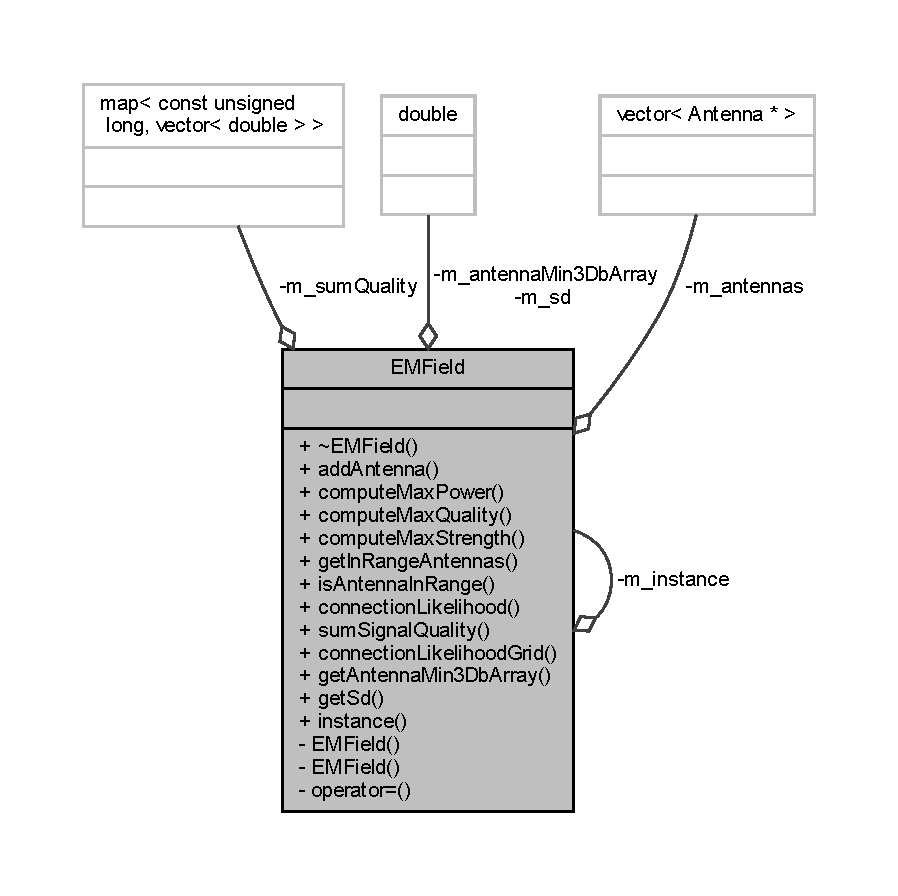
\includegraphics[width=350pt]{class_e_m_field__coll__graph}
\end{center}
\end{figure}
\doxysubsection*{Public Member Functions}
\begin{DoxyCompactItemize}
\item 
virtual \mbox{\hyperlink{class_e_m_field_abe7db07a27a120858107d5efa5f14edb}{$\sim$\+E\+M\+Field}} ()
\item 
void \mbox{\hyperlink{class_e_m_field_ac531ecbce4c81aa5da19fe3c734a585c}{add\+Antenna}} (\mbox{\hyperlink{class_antenna}{Antenna}} $\ast$a)
\item 
pair$<$ \mbox{\hyperlink{class_antenna}{Antenna}} $\ast$, double $>$ \mbox{\hyperlink{class_e_m_field_a01cfb9fea3dadfcfe5d6f00551193acd}{compute\+Max\+Power}} (const Point $\ast$p, const unsigned long mno\+Id)
\item 
pair$<$ \mbox{\hyperlink{class_antenna}{Antenna}} $\ast$, double $>$ \mbox{\hyperlink{class_e_m_field_ac866f6224e34895a0ee085c4baf43a01}{compute\+Max\+Quality}} (const Point $\ast$p, const unsigned long mno\+Id)
\item 
pair$<$ \mbox{\hyperlink{class_antenna}{Antenna}} $\ast$, double $>$ \mbox{\hyperlink{class_e_m_field_a9a3cdbca4fcf408ce58a30fb98de1bbb}{compute\+Max\+Strength}} (const Point $\ast$p, const unsigned long mno\+Id)
\item 
vector$<$ pair$<$ \mbox{\hyperlink{class_antenna}{Antenna}} $\ast$, double $>$ $>$ \mbox{\hyperlink{class_e_m_field_a2ad800417b06a62e68edd1fccb5c4b93}{get\+In\+Range\+Antennas}} (const Point $\ast$p, const double threshold, const \mbox{\hyperlink{class_holdable_agent_ae2c334b004d7b9c5a999cf2618e4e518}{Holdable\+Agent\+::\+C\+O\+N\+N\+E\+C\+T\+I\+O\+N\+\_\+\+T\+Y\+PE}} conn\+Type, unsigned long mno\+Id)
\item 
bool \mbox{\hyperlink{class_e_m_field_a5cd43aded41779d2d24de3f3e5c717d0}{is\+Antenna\+In\+Range}} (const Point $\ast$p, \mbox{\hyperlink{class_antenna}{Antenna}} $\ast$a, const double threshold, const \mbox{\hyperlink{class_holdable_agent_ae2c334b004d7b9c5a999cf2618e4e518}{Holdable\+Agent\+::\+C\+O\+N\+N\+E\+C\+T\+I\+O\+N\+\_\+\+T\+Y\+PE}} conn\+Type)
\item 
double \mbox{\hyperlink{class_e_m_field_a710da64db53718cdeed7b8c8dc11bba3}{connection\+Likelihood}} (\mbox{\hyperlink{class_antenna}{Antenna}} $\ast$a, const Point $\ast$p)
\item 
vector$<$ double $>$ \mbox{\hyperlink{class_e_m_field_acef16c598b62605a691f75f99d364447}{sum\+Signal\+Quality}} (const \mbox{\hyperlink{class_map}{Map}} $\ast$map, const unsigned long mno\+ID)
\item 
double \mbox{\hyperlink{class_e_m_field_a6a4a10f9a013ab994eccb1ec10c0a180}{connection\+Likelihood\+Grid}} (\mbox{\hyperlink{class_antenna}{Antenna}} $\ast$a, const \mbox{\hyperlink{class_map}{Map}} $\ast$map, unsigned long tile\+Index)
\item 
const double $\ast$ \mbox{\hyperlink{class_e_m_field_ab2132484b9c52f2224bc81f354b24df6}{get\+Antenna\+Min3\+Db\+Array}} () const
\item 
double $\ast$ \mbox{\hyperlink{class_e_m_field_a0fea003948a67df01174480480376169}{get\+Sd}} () const
\end{DoxyCompactItemize}
\doxysubsection*{Static Public Member Functions}
\begin{DoxyCompactItemize}
\item 
static \mbox{\hyperlink{class_e_m_field}{E\+M\+Field}} $\ast$ \mbox{\hyperlink{class_e_m_field_acbadbede116ac320398cbfcd19e90ec7}{instance}} ()
\end{DoxyCompactItemize}
\doxysubsection*{Private Member Functions}
\begin{DoxyCompactItemize}
\item 
\mbox{\hyperlink{class_e_m_field_a054f389cfa853008f32c02d874aa4d58}{E\+M\+Field}} ()
\item 
\mbox{\hyperlink{class_e_m_field_a7760631ded36ba2c5a918c97a1cc93e9}{E\+M\+Field}} (const \mbox{\hyperlink{class_e_m_field}{E\+M\+Field}} \&)
\item 
\mbox{\hyperlink{class_e_m_field}{E\+M\+Field}} \& \mbox{\hyperlink{class_e_m_field_ad35e4754cad2016d7df1b8ac45540b35}{operator=}} (const \mbox{\hyperlink{class_e_m_field}{E\+M\+Field}} \&)
\end{DoxyCompactItemize}
\doxysubsection*{Private Attributes}
\begin{DoxyCompactItemize}
\item 
vector$<$ \mbox{\hyperlink{class_antenna}{Antenna}} $\ast$ $>$ \mbox{\hyperlink{class_e_m_field_ab74a3bde70b66fd033bde6c25345a755}{m\+\_\+antennas}}
\item 
map$<$ const unsigned long, vector$<$ double $>$ $>$ \mbox{\hyperlink{class_e_m_field_a18e5a4d972d888c5da458e30e426c7ae}{m\+\_\+sum\+Quality}}
\item 
double $\ast$ \mbox{\hyperlink{class_e_m_field_a96c4c7bc39c2f8afea0dca3280fe145c}{m\+\_\+antenna\+Min3\+Db\+Array}}
\item 
double $\ast$ \mbox{\hyperlink{class_e_m_field_ac2142eafd5b82e43437a8047565f619c}{m\+\_\+sd}}
\end{DoxyCompactItemize}
\doxysubsection*{Static Private Attributes}
\begin{DoxyCompactItemize}
\item 
static \mbox{\hyperlink{class_e_m_field}{E\+M\+Field}} $\ast$ \mbox{\hyperlink{class_e_m_field_a3a75e412fa15cfab78ce64dfbb8af52d}{m\+\_\+instance}}
\end{DoxyCompactItemize}


\doxysubsection{Detailed Description}
This utility singleton class is used to compute different measures of the electromagnetic field radiated by an antenna (power, signal strength etc) and it also provides methods needed to decide to which antenna a mobile device connects. 

\doxysubsection{Constructor \& Destructor Documentation}
\mbox{\Hypertarget{class_e_m_field_abe7db07a27a120858107d5efa5f14edb}\label{class_e_m_field_abe7db07a27a120858107d5efa5f14edb}} 
\index{EMField@{EMField}!````~EMField@{$\sim$EMField}}
\index{````~EMField@{$\sim$EMField}!EMField@{EMField}}
\doxysubsubsection{\texorpdfstring{$\sim$EMField()}{~EMField()}}
{\footnotesize\ttfamily virtual E\+M\+Field\+::$\sim$\+E\+M\+Field (\begin{DoxyParamCaption}{ }\end{DoxyParamCaption})\hspace{0.3cm}{\ttfamily [virtual]}}

Default destructor. \mbox{\Hypertarget{class_e_m_field_a054f389cfa853008f32c02d874aa4d58}\label{class_e_m_field_a054f389cfa853008f32c02d874aa4d58}} 
\index{EMField@{EMField}!EMField@{EMField}}
\index{EMField@{EMField}!EMField@{EMField}}
\doxysubsubsection{\texorpdfstring{EMField()}{EMField()}\hspace{0.1cm}{\footnotesize\ttfamily [1/2]}}
{\footnotesize\ttfamily E\+M\+Field\+::\+E\+M\+Field (\begin{DoxyParamCaption}{ }\end{DoxyParamCaption})\hspace{0.3cm}{\ttfamily [private]}}

\mbox{\Hypertarget{class_e_m_field_a7760631ded36ba2c5a918c97a1cc93e9}\label{class_e_m_field_a7760631ded36ba2c5a918c97a1cc93e9}} 
\index{EMField@{EMField}!EMField@{EMField}}
\index{EMField@{EMField}!EMField@{EMField}}
\doxysubsubsection{\texorpdfstring{EMField()}{EMField()}\hspace{0.1cm}{\footnotesize\ttfamily [2/2]}}
{\footnotesize\ttfamily E\+M\+Field\+::\+E\+M\+Field (\begin{DoxyParamCaption}\item[{const \mbox{\hyperlink{class_e_m_field}{E\+M\+Field}} \&}]{ }\end{DoxyParamCaption})\hspace{0.3cm}{\ttfamily [private]}}



\doxysubsection{Member Function Documentation}
\mbox{\Hypertarget{class_e_m_field_ac531ecbce4c81aa5da19fe3c734a585c}\label{class_e_m_field_ac531ecbce4c81aa5da19fe3c734a585c}} 
\index{EMField@{EMField}!addAntenna@{addAntenna}}
\index{addAntenna@{addAntenna}!EMField@{EMField}}
\doxysubsubsection{\texorpdfstring{addAntenna()}{addAntenna()}}
{\footnotesize\ttfamily void E\+M\+Field\+::add\+Antenna (\begin{DoxyParamCaption}\item[{\mbox{\hyperlink{class_antenna}{Antenna}} $\ast$}]{a }\end{DoxyParamCaption})}

Add a pointer to an \mbox{\hyperlink{class_antenna}{Antenna}} object to an internal collection needed for computations. Although these pointers are kept in an Agent\+Collection object they are also added to a local vector in this class for performance reasons. 
\begin{DoxyParams}{Parameters}
{\em a} & a pointer to the \mbox{\hyperlink{class_antenna}{Antenna}} object \\
\hline
\end{DoxyParams}
\mbox{\Hypertarget{class_e_m_field_a01cfb9fea3dadfcfe5d6f00551193acd}\label{class_e_m_field_a01cfb9fea3dadfcfe5d6f00551193acd}} 
\index{EMField@{EMField}!computeMaxPower@{computeMaxPower}}
\index{computeMaxPower@{computeMaxPower}!EMField@{EMField}}
\doxysubsubsection{\texorpdfstring{computeMaxPower()}{computeMaxPower()}}
{\footnotesize\ttfamily pair$<$\mbox{\hyperlink{class_antenna}{Antenna}}$\ast$, double$>$ E\+M\+Field\+::compute\+Max\+Power (\begin{DoxyParamCaption}\item[{const Point $\ast$}]{p,  }\item[{const unsigned long}]{mno\+Id }\end{DoxyParamCaption})}

Returns a pair made of a pointer to an \mbox{\hyperlink{class_antenna}{Antenna}} object and its power with the property that in the location specified by parameter p, the \mbox{\hyperlink{class_antenna}{Antenna}} returned by this method provides the highest power (the power of the field is considered to decrease according a power-\/law). 
\begin{DoxyParams}{Parameters}
{\em p} & the location where we want to find which \mbox{\hyperlink{class_antenna}{Antenna}} provides the highest power the of electromagnetic field. \\
\hline
{\em mno\+Id} & the id of the M\+NO for which we compute the power. Only antennas belonging to this M\+NO will be considered during computations. \\
\hline
\end{DoxyParams}
\begin{DoxyReturn}{Returns}
a pair$<$\+Antenna$\ast$, double$>$ containing a pointer to the \mbox{\hyperlink{class_antenna}{Antenna}} object that provides the highest power of the field in the location specified by p. 
\end{DoxyReturn}
\mbox{\Hypertarget{class_e_m_field_ac866f6224e34895a0ee085c4baf43a01}\label{class_e_m_field_ac866f6224e34895a0ee085c4baf43a01}} 
\index{EMField@{EMField}!computeMaxQuality@{computeMaxQuality}}
\index{computeMaxQuality@{computeMaxQuality}!EMField@{EMField}}
\doxysubsubsection{\texorpdfstring{computeMaxQuality()}{computeMaxQuality()}}
{\footnotesize\ttfamily pair$<$\mbox{\hyperlink{class_antenna}{Antenna}}$\ast$, double$>$ E\+M\+Field\+::compute\+Max\+Quality (\begin{DoxyParamCaption}\item[{const Point $\ast$}]{p,  }\item[{const unsigned long}]{mno\+Id }\end{DoxyParamCaption})}

Returns a pair made of a pointer to an \mbox{\hyperlink{class_antenna}{Antenna}} object and its signal quality with the property that in the location specified by p, the \mbox{\hyperlink{class_antenna}{Antenna}} returned by this method provides signal with the highest quality. The signal quality in this pair is the computed in location given by p. 
\begin{DoxyParams}{Parameters}
{\em p} & indicates the location where we want to find which \mbox{\hyperlink{class_antenna}{Antenna}} provides the highest quality of the signal. \\
\hline
{\em mno\+Id} & the id of the M\+NO for which we compute the signal quality. Only antennas belonging to this M\+NO will be considered during computations. \\
\hline
\end{DoxyParams}
\begin{DoxyReturn}{Returns}
a pair$<$\+Antenna$\ast$, double$>$ containing a pointer to the \mbox{\hyperlink{class_antenna}{Antenna}} object that provides a signal with the highest quality in location given by p. 
\end{DoxyReturn}
\mbox{\Hypertarget{class_e_m_field_a9a3cdbca4fcf408ce58a30fb98de1bbb}\label{class_e_m_field_a9a3cdbca4fcf408ce58a30fb98de1bbb}} 
\index{EMField@{EMField}!computeMaxStrength@{computeMaxStrength}}
\index{computeMaxStrength@{computeMaxStrength}!EMField@{EMField}}
\doxysubsubsection{\texorpdfstring{computeMaxStrength()}{computeMaxStrength()}}
{\footnotesize\ttfamily pair$<$\mbox{\hyperlink{class_antenna}{Antenna}}$\ast$, double$>$ E\+M\+Field\+::compute\+Max\+Strength (\begin{DoxyParamCaption}\item[{const Point $\ast$}]{p,  }\item[{const unsigned long}]{mno\+Id }\end{DoxyParamCaption})}

Returns a pair made of a pointer to an \mbox{\hyperlink{class_antenna}{Antenna}} object and its signal strength with the property that in the location specified by p, the \mbox{\hyperlink{class_antenna}{Antenna}} returned by this method provides signal with the highest strength. The signal strength in this pair is the computed in location given by p. 
\begin{DoxyParams}{Parameters}
{\em p} & indicates the location where we want to find which \mbox{\hyperlink{class_antenna}{Antenna}} provides the highest strength of the signal. \\
\hline
{\em mno\+Id} & the id of the M\+NO for which we compute the signal strength. Only antennas belonging to this M\+NO will be considered during computations. \\
\hline
\end{DoxyParams}
\begin{DoxyReturn}{Returns}
a pair$<$\+Antenna$\ast$, double$>$ containing a pointer to the \mbox{\hyperlink{class_antenna}{Antenna}} object that provides a signal with the highest strength in location given by p. 
\end{DoxyReturn}
\mbox{\Hypertarget{class_e_m_field_a710da64db53718cdeed7b8c8dc11bba3}\label{class_e_m_field_a710da64db53718cdeed7b8c8dc11bba3}} 
\index{EMField@{EMField}!connectionLikelihood@{connectionLikelihood}}
\index{connectionLikelihood@{connectionLikelihood}!EMField@{EMField}}
\doxysubsubsection{\texorpdfstring{connectionLikelihood()}{connectionLikelihood()}}
{\footnotesize\ttfamily double E\+M\+Field\+::connection\+Likelihood (\begin{DoxyParamCaption}\item[{\mbox{\hyperlink{class_antenna}{Antenna}} $\ast$}]{a,  }\item[{const Point $\ast$}]{p }\end{DoxyParamCaption})}

Computes the connection likelihood for \mbox{\hyperlink{class_antenna}{Antenna}} indicated by a in a certain location given by p. The connection likelihood is computed dividing the signal quality provided by \mbox{\hyperlink{class_antenna}{Antenna}} indicated through p by the sum of the signal quality provided by all antennas of an M\+NO. 
\begin{DoxyParams}{Parameters}
{\em a} & a pointer to an \mbox{\hyperlink{class_antenna}{Antenna}} object. \\
\hline
{\em p} & a location in space. \\
\hline
\end{DoxyParams}
\begin{DoxyReturn}{Returns}
the connection likelihood for \mbox{\hyperlink{class_antenna}{Antenna}} a in location p. 
\end{DoxyReturn}
\mbox{\Hypertarget{class_e_m_field_a6a4a10f9a013ab994eccb1ec10c0a180}\label{class_e_m_field_a6a4a10f9a013ab994eccb1ec10c0a180}} 
\index{EMField@{EMField}!connectionLikelihoodGrid@{connectionLikelihoodGrid}}
\index{connectionLikelihoodGrid@{connectionLikelihoodGrid}!EMField@{EMField}}
\doxysubsubsection{\texorpdfstring{connectionLikelihoodGrid()}{connectionLikelihoodGrid()}}
{\footnotesize\ttfamily double E\+M\+Field\+::connection\+Likelihood\+Grid (\begin{DoxyParamCaption}\item[{\mbox{\hyperlink{class_antenna}{Antenna}} $\ast$}]{a,  }\item[{const \mbox{\hyperlink{class_map}{Map}} $\ast$}]{map,  }\item[{unsigned long}]{tile\+Index }\end{DoxyParamCaption})}

Computes the connection likelihood for \mbox{\hyperlink{class_antenna}{Antenna}} indicated by a in the center of the tile indicated by tile\+Index 
\begin{DoxyParams}{Parameters}
{\em a} & a pointer to an \mbox{\hyperlink{class_antenna}{Antenna}} object. \\
\hline
{\em map} & a pointer to the map of the simulation. \\
\hline
{\em tile\+Index} & the index of the tile where we want to compute the connection likelihood. \\
\hline
\end{DoxyParams}
\begin{DoxyReturn}{Returns}
the connection likelihood for \mbox{\hyperlink{class_antenna}{Antenna}} a in the center of the tile with the index tile\+Index. 
\end{DoxyReturn}
\mbox{\Hypertarget{class_e_m_field_ab2132484b9c52f2224bc81f354b24df6}\label{class_e_m_field_ab2132484b9c52f2224bc81f354b24df6}} 
\index{EMField@{EMField}!getAntennaMin3DbArray@{getAntennaMin3DbArray}}
\index{getAntennaMin3DbArray@{getAntennaMin3DbArray}!EMField@{EMField}}
\doxysubsubsection{\texorpdfstring{getAntennaMin3DbArray()}{getAntennaMin3DbArray()}}
{\footnotesize\ttfamily const double$\ast$ E\+M\+Field\+::get\+Antenna\+Min3\+Db\+Array (\begin{DoxyParamCaption}{ }\end{DoxyParamCaption}) const}

\mbox{\Hypertarget{class_e_m_field_a2ad800417b06a62e68edd1fccb5c4b93}\label{class_e_m_field_a2ad800417b06a62e68edd1fccb5c4b93}} 
\index{EMField@{EMField}!getInRangeAntennas@{getInRangeAntennas}}
\index{getInRangeAntennas@{getInRangeAntennas}!EMField@{EMField}}
\doxysubsubsection{\texorpdfstring{getInRangeAntennas()}{getInRangeAntennas()}}
{\footnotesize\ttfamily vector$<$pair$<$\mbox{\hyperlink{class_antenna}{Antenna}}$\ast$, double$>$ $>$ E\+M\+Field\+::get\+In\+Range\+Antennas (\begin{DoxyParamCaption}\item[{const Point $\ast$}]{p,  }\item[{const double}]{threshold,  }\item[{const \mbox{\hyperlink{class_holdable_agent_ae2c334b004d7b9c5a999cf2618e4e518}{Holdable\+Agent\+::\+C\+O\+N\+N\+E\+C\+T\+I\+O\+N\+\_\+\+T\+Y\+PE}}}]{conn\+Type,  }\item[{unsigned long}]{mno\+Id }\end{DoxyParamCaption})}

Returns a vector of pairs made up of a pointer to an \mbox{\hyperlink{class_antenna}{Antenna}} object and its power, signal quality or signal strength. All the antennas in this vector provides a signal with a power or signal quality greater than the threshold provided as threshold, i.\+e. this vector contains all antennas that have in their coverage area the location given by point p. 
\begin{DoxyParams}{Parameters}
{\em p} & the location where we want to have the list with the all antennas that covers it. \\
\hline
{\em threshold} & the lowest limit of the power or signal quality below which the signal is considered to be only noise, i.\+e. it defines the limit of the coverage area. \\
\hline
{\em conn\+Type} & indicates the mechanism used to set up a connection between an antenna and a mobile phone \\
\hline
{\em mno\+Id} & the id of the M\+NO for which we build the resulting vector. Only antennas belonging to this M\+NO will be considered during computations. \\
\hline
\end{DoxyParams}
\begin{DoxyReturn}{Returns}
a vector of pairs made up of a pointer to an \mbox{\hyperlink{class_antenna}{Antenna}} object and its power, signal quality or signal strength, according to the value of the conn\+Type. All the antennas in this vector provides a signal with a power, signal quality or signal strength greater than the threshold. 
\end{DoxyReturn}
\mbox{\Hypertarget{class_e_m_field_a0fea003948a67df01174480480376169}\label{class_e_m_field_a0fea003948a67df01174480480376169}} 
\index{EMField@{EMField}!getSd@{getSd}}
\index{getSd@{getSd}!EMField@{EMField}}
\doxysubsubsection{\texorpdfstring{getSd()}{getSd()}}
{\footnotesize\ttfamily double$\ast$ E\+M\+Field\+::get\+Sd (\begin{DoxyParamCaption}{ }\end{DoxyParamCaption}) const}

\mbox{\Hypertarget{class_e_m_field_acbadbede116ac320398cbfcd19e90ec7}\label{class_e_m_field_acbadbede116ac320398cbfcd19e90ec7}} 
\index{EMField@{EMField}!instance@{instance}}
\index{instance@{instance}!EMField@{EMField}}
\doxysubsubsection{\texorpdfstring{instance()}{instance()}}
{\footnotesize\ttfamily static \mbox{\hyperlink{class_e_m_field}{E\+M\+Field}}$\ast$ E\+M\+Field\+::instance (\begin{DoxyParamCaption}{ }\end{DoxyParamCaption})\hspace{0.3cm}{\ttfamily [inline]}, {\ttfamily [static]}}

Returns an instance of this class. This class is a singleton. \begin{DoxyReturn}{Returns}
an instance of this class. 
\end{DoxyReturn}
\mbox{\Hypertarget{class_e_m_field_a5cd43aded41779d2d24de3f3e5c717d0}\label{class_e_m_field_a5cd43aded41779d2d24de3f3e5c717d0}} 
\index{EMField@{EMField}!isAntennaInRange@{isAntennaInRange}}
\index{isAntennaInRange@{isAntennaInRange}!EMField@{EMField}}
\doxysubsubsection{\texorpdfstring{isAntennaInRange()}{isAntennaInRange()}}
{\footnotesize\ttfamily bool E\+M\+Field\+::is\+Antenna\+In\+Range (\begin{DoxyParamCaption}\item[{const Point $\ast$}]{p,  }\item[{\mbox{\hyperlink{class_antenna}{Antenna}} $\ast$}]{a,  }\item[{const double}]{threshold,  }\item[{const \mbox{\hyperlink{class_holdable_agent_ae2c334b004d7b9c5a999cf2618e4e518}{Holdable\+Agent\+::\+C\+O\+N\+N\+E\+C\+T\+I\+O\+N\+\_\+\+T\+Y\+PE}}}]{conn\+Type }\end{DoxyParamCaption})}

Checks if p is in the coverage area of \mbox{\hyperlink{class_antenna}{Antenna}} pointed out by a. The coverage area is considered the area where the signal quality or the power of the field is greater than the value of threshold. 
\begin{DoxyParams}{Parameters}
{\em p} & the location that we want to check the power or the quality of the signal \\
\hline
{\em a} & pointer to an \mbox{\hyperlink{class_antenna}{Antenna}} object for which we want to check if it covers the point p. \\
\hline
{\em threshold} & the lower limit of the power or signal quality below which the signal is considered only noise. \\
\hline
{\em conn\+Type} & indicates the mechanism used to set up a connection between an antenna and a mobile phone. \\
\hline
\end{DoxyParams}
\begin{DoxyReturn}{Returns}
true is the \mbox{\hyperlink{class_antenna}{Antenna}} object provide enough power or signal quality in the location given as p. 
\end{DoxyReturn}
\mbox{\Hypertarget{class_e_m_field_ad35e4754cad2016d7df1b8ac45540b35}\label{class_e_m_field_ad35e4754cad2016d7df1b8ac45540b35}} 
\index{EMField@{EMField}!operator=@{operator=}}
\index{operator=@{operator=}!EMField@{EMField}}
\doxysubsubsection{\texorpdfstring{operator=()}{operator=()}}
{\footnotesize\ttfamily \mbox{\hyperlink{class_e_m_field}{E\+M\+Field}}\& E\+M\+Field\+::operator= (\begin{DoxyParamCaption}\item[{const \mbox{\hyperlink{class_e_m_field}{E\+M\+Field}} \&}]{ }\end{DoxyParamCaption})\hspace{0.3cm}{\ttfamily [private]}}

\mbox{\Hypertarget{class_e_m_field_acef16c598b62605a691f75f99d364447}\label{class_e_m_field_acef16c598b62605a691f75f99d364447}} 
\index{EMField@{EMField}!sumSignalQuality@{sumSignalQuality}}
\index{sumSignalQuality@{sumSignalQuality}!EMField@{EMField}}
\doxysubsubsection{\texorpdfstring{sumSignalQuality()}{sumSignalQuality()}}
{\footnotesize\ttfamily vector$<$double$>$ E\+M\+Field\+::sum\+Signal\+Quality (\begin{DoxyParamCaption}\item[{const \mbox{\hyperlink{class_map}{Map}} $\ast$}]{map,  }\item[{const unsigned long}]{mno\+ID }\end{DoxyParamCaption})}

Computes the sum of the signal quality given by all antennas belonging to an M\+NO for all tiles in the reference grid. The signal quality is computed in the center of each tile. 
\begin{DoxyParams}{Parameters}
{\em map} & the of the simulation. It is needed to extract the grid of tiles where this method computes the sum of the signal quality. This grid is set at the beginning of the simulation and it overlaps the \mbox{\hyperlink{class_map}{Map}}. \\
\hline
{\em mno\+ID} & the id of the M\+NO for which we want to compute this sum. \\
\hline
\end{DoxyParams}
\begin{DoxyReturn}{Returns}
a vector containing the sum of the signal quality given by all antennas of an M\+NO, for all tiles in the reference grid. An element of the vector corresponds to a tile in the grid. The tiles are linearized in a row-\/major order starting with the bottom-\/left corner. 
\end{DoxyReturn}


\doxysubsection{Member Data Documentation}
\mbox{\Hypertarget{class_e_m_field_a96c4c7bc39c2f8afea0dca3280fe145c}\label{class_e_m_field_a96c4c7bc39c2f8afea0dca3280fe145c}} 
\index{EMField@{EMField}!m\_antennaMin3DbArray@{m\_antennaMin3DbArray}}
\index{m\_antennaMin3DbArray@{m\_antennaMin3DbArray}!EMField@{EMField}}
\doxysubsubsection{\texorpdfstring{m\_antennaMin3DbArray}{m\_antennaMin3DbArray}}
{\footnotesize\ttfamily double$\ast$ E\+M\+Field\+::m\+\_\+antenna\+Min3\+Db\+Array\hspace{0.3cm}{\ttfamily [private]}}

\mbox{\Hypertarget{class_e_m_field_ab74a3bde70b66fd033bde6c25345a755}\label{class_e_m_field_ab74a3bde70b66fd033bde6c25345a755}} 
\index{EMField@{EMField}!m\_antennas@{m\_antennas}}
\index{m\_antennas@{m\_antennas}!EMField@{EMField}}
\doxysubsubsection{\texorpdfstring{m\_antennas}{m\_antennas}}
{\footnotesize\ttfamily vector$<$\mbox{\hyperlink{class_antenna}{Antenna}}$\ast$$>$ E\+M\+Field\+::m\+\_\+antennas\hspace{0.3cm}{\ttfamily [private]}}

\mbox{\Hypertarget{class_e_m_field_a3a75e412fa15cfab78ce64dfbb8af52d}\label{class_e_m_field_a3a75e412fa15cfab78ce64dfbb8af52d}} 
\index{EMField@{EMField}!m\_instance@{m\_instance}}
\index{m\_instance@{m\_instance}!EMField@{EMField}}
\doxysubsubsection{\texorpdfstring{m\_instance}{m\_instance}}
{\footnotesize\ttfamily \mbox{\hyperlink{class_e_m_field}{E\+M\+Field}}$\ast$ E\+M\+Field\+::m\+\_\+instance\hspace{0.3cm}{\ttfamily [static]}, {\ttfamily [private]}}

\mbox{\Hypertarget{class_e_m_field_ac2142eafd5b82e43437a8047565f619c}\label{class_e_m_field_ac2142eafd5b82e43437a8047565f619c}} 
\index{EMField@{EMField}!m\_sd@{m\_sd}}
\index{m\_sd@{m\_sd}!EMField@{EMField}}
\doxysubsubsection{\texorpdfstring{m\_sd}{m\_sd}}
{\footnotesize\ttfamily double$\ast$ E\+M\+Field\+::m\+\_\+sd\hspace{0.3cm}{\ttfamily [private]}}

\mbox{\Hypertarget{class_e_m_field_a18e5a4d972d888c5da458e30e426c7ae}\label{class_e_m_field_a18e5a4d972d888c5da458e30e426c7ae}} 
\index{EMField@{EMField}!m\_sumQuality@{m\_sumQuality}}
\index{m\_sumQuality@{m\_sumQuality}!EMField@{EMField}}
\doxysubsubsection{\texorpdfstring{m\_sumQuality}{m\_sumQuality}}
{\footnotesize\ttfamily map$<$const unsigned long, vector$<$double$>$ $>$ E\+M\+Field\+::m\+\_\+sum\+Quality\hspace{0.3cm}{\ttfamily [private]}}



The documentation for this class was generated from the following file\+:\begin{DoxyCompactItemize}
\item 
include/\mbox{\hyperlink{_e_m_field_8h}{E\+M\+Field.\+h}}\end{DoxyCompactItemize}

\hypertarget{class_event_factory}{}\doxysection{Event\+Factory Class Reference}
\label{class_event_factory}\index{EventFactory@{EventFactory}}


{\ttfamily \#include $<$Event\+Factory.\+h$>$}



Collaboration diagram for Event\+Factory\+:\nopagebreak
\begin{figure}[H]
\begin{center}
\leavevmode
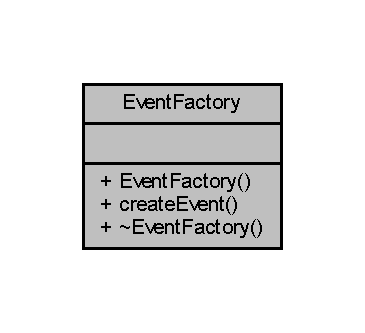
\includegraphics[width=175pt]{class_event_factory__coll__graph}
\end{center}
\end{figure}
\doxysubsection*{Public Member Functions}
\begin{DoxyCompactItemize}
\item 
\mbox{\hyperlink{class_event_factory_a67f3a225f757c461fef45f0141a37f61}{Event\+Factory}} ()
\item 
\mbox{\hyperlink{class_event}{Event}} $\ast$ \mbox{\hyperlink{class_event_factory_ad1e99b5e55dede758da8e09cc976ae01}{create\+Event}} (\mbox{\hyperlink{class_event_config}{Event\+Config}} $\ast$config)
\item 
virtual \mbox{\hyperlink{class_event_factory_a94604de7384acdb8c5aafc0d31e41e28}{$\sim$\+Event\+Factory}} ()
\end{DoxyCompactItemize}


\doxysubsection{Detailed Description}
This is the factory class that builds different types of network events according to the configuration of the simulator. 

\doxysubsection{Constructor \& Destructor Documentation}
\mbox{\Hypertarget{class_event_factory_a67f3a225f757c461fef45f0141a37f61}\label{class_event_factory_a67f3a225f757c461fef45f0141a37f61}} 
\index{EventFactory@{EventFactory}!EventFactory@{EventFactory}}
\index{EventFactory@{EventFactory}!EventFactory@{EventFactory}}
\doxysubsubsection{\texorpdfstring{EventFactory()}{EventFactory()}}
{\footnotesize\ttfamily Event\+Factory\+::\+Event\+Factory (\begin{DoxyParamCaption}{ }\end{DoxyParamCaption})}

Default constructor \mbox{\Hypertarget{class_event_factory_a94604de7384acdb8c5aafc0d31e41e28}\label{class_event_factory_a94604de7384acdb8c5aafc0d31e41e28}} 
\index{EventFactory@{EventFactory}!````~EventFactory@{$\sim$EventFactory}}
\index{````~EventFactory@{$\sim$EventFactory}!EventFactory@{EventFactory}}
\doxysubsubsection{\texorpdfstring{$\sim$EventFactory()}{~EventFactory()}}
{\footnotesize\ttfamily virtual Event\+Factory\+::$\sim$\+Event\+Factory (\begin{DoxyParamCaption}{ }\end{DoxyParamCaption})\hspace{0.3cm}{\ttfamily [virtual]}}

Default destructor. 

\doxysubsection{Member Function Documentation}
\mbox{\Hypertarget{class_event_factory_ad1e99b5e55dede758da8e09cc976ae01}\label{class_event_factory_ad1e99b5e55dede758da8e09cc976ae01}} 
\index{EventFactory@{EventFactory}!createEvent@{createEvent}}
\index{createEvent@{createEvent}!EventFactory@{EventFactory}}
\doxysubsubsection{\texorpdfstring{createEvent()}{createEvent()}}
{\footnotesize\ttfamily \mbox{\hyperlink{class_event}{Event}}$\ast$ Event\+Factory\+::create\+Event (\begin{DoxyParamCaption}\item[{\mbox{\hyperlink{class_event_config}{Event\+Config}} $\ast$}]{config }\end{DoxyParamCaption})}

Creates a concrete \mbox{\hyperlink{class_event}{Event}} object according to the actual type of the {\ttfamily config} argument. Two types of events are implemented\+: \mbox{\hyperlink{class_cell_i_d_event}{Cell\+I\+D\+Event}} and \mbox{\hyperlink{class_cell_i_d_t_a_event}{Cell\+I\+D\+T\+A\+Event}}. \mbox{\hyperlink{class_cell_i_d_event}{Cell\+I\+D\+Event}} contains the ID of the cell where a mobile device was detected at a time instant, the network type and the timestamp of the event and the \mbox{\hyperlink{class_cell_i_d_t_a_event}{Cell\+I\+D\+T\+A\+Event}} additionally contains the timing advance value of the event. \begin{DoxyReturn}{Returns}
a pointer to a concrete \mbox{\hyperlink{class_event}{Event}} object created according to the actual type of the of the {\ttfamily config} argument. The two types of event objects supported are\+: \begin{DoxyItemize}
\item \mbox{\hyperlink{class_cell_i_d_event}{Cell\+I\+D\+Event}} and in this case the {\ttfamily config} parameter should point to a Cell\+I\+D\+Eventconfig object \item \mbox{\hyperlink{class_cell_i_d_t_a_event}{Cell\+I\+D\+T\+A\+Event}} and in this case the {\ttfamily config} parameter should point to a Cell\+I\+D\+T\+A\+Eventconfig object. \end{DoxyItemize}

\end{DoxyReturn}


The documentation for this class was generated from the following file\+:\begin{DoxyCompactItemize}
\item 
include/events/\mbox{\hyperlink{_event_factory_8h}{Event\+Factory.\+h}}\end{DoxyCompactItemize}

\hypertarget{classexception}{}\doxysection{exception Class Reference}
\label{classexception}\index{exception@{exception}}


Inheritance diagram for exception\+:\nopagebreak
\begin{figure}[H]
\begin{center}
\leavevmode
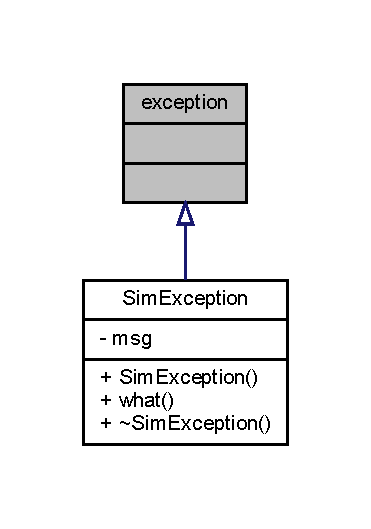
\includegraphics[width=178pt]{classexception__inherit__graph}
\end{center}
\end{figure}


Collaboration diagram for exception\+:\nopagebreak
\begin{figure}[H]
\begin{center}
\leavevmode
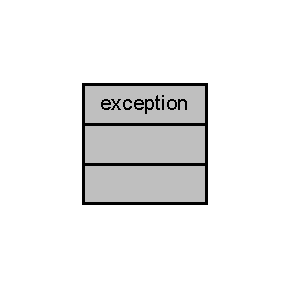
\includegraphics[width=139pt]{classexception__coll__graph}
\end{center}
\end{figure}


The documentation for this class was generated from the following file\+:\begin{DoxyCompactItemize}
\item 
include/\mbox{\hyperlink{_sim_exception_8h}{Sim\+Exception.\+h}}\end{DoxyCompactItemize}

\hypertarget{class_grid}{}\section{Grid Class Reference}
\label{class_grid}\index{Grid@{Grid}}


{\ttfamily \#include $<$Grid.\+h$>$}



Collaboration diagram for Grid\+:\nopagebreak
\begin{figure}[H]
\begin{center}
\leavevmode
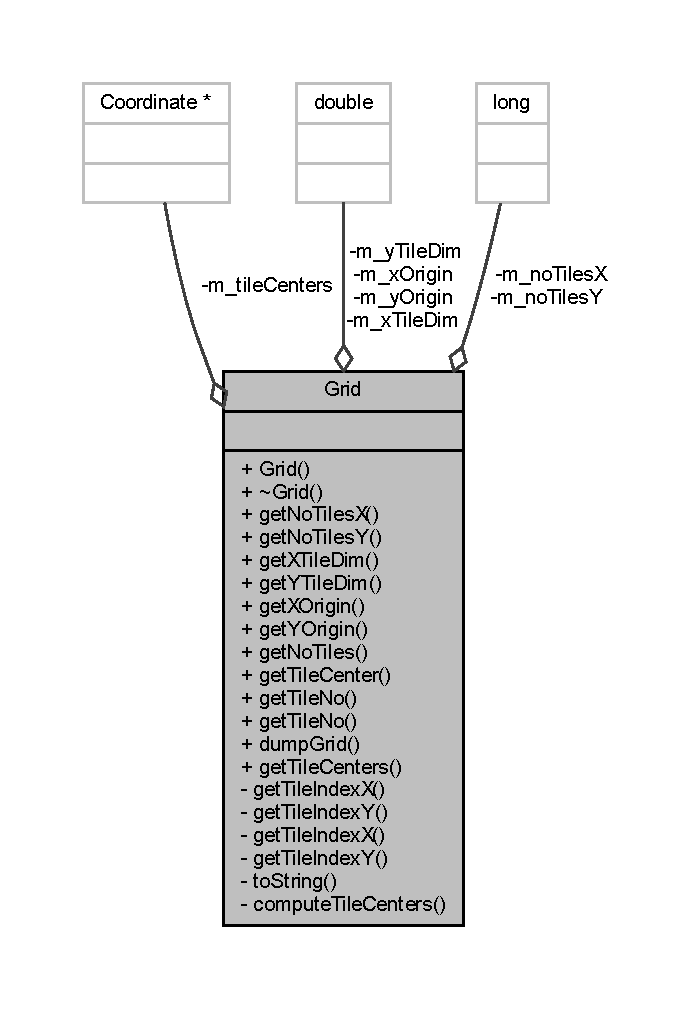
\includegraphics[width=331pt]{class_grid__coll__graph}
\end{center}
\end{figure}
\subsection*{Public Member Functions}
\begin{DoxyCompactItemize}
\item 
\hyperlink{class_grid_a84b0dc169028f21175a4549afde86153}{Grid} (double x\+Orig, double y\+Orig, double x\+Tiledim, double y\+Tiledim, unsigned long no\+TilesX, unsigned long no\+TilesY)
\item 
virtual \hyperlink{class_grid_a241c623291936ddbf4f670a796523a91}{$\sim$\+Grid} ()
\item 
unsigned long \hyperlink{class_grid_af29c0c404a908aa46f83afb17d7609a6}{get\+No\+TilesX} () const
\item 
unsigned long \hyperlink{class_grid_a783a3153d03154cfd33e6a418bb8d390}{get\+No\+TilesY} () const
\item 
double \hyperlink{class_grid_a1c5b9ad91fac264bcdd67f99bc93f663}{get\+X\+Tile\+Dim} () const
\item 
double \hyperlink{class_grid_aedfe477f5be79a375bd64a4d21765918}{get\+Y\+Tile\+Dim} () const
\item 
double \hyperlink{class_grid_a08b534c7f8e1099a6903bf08d9727842}{get\+X\+Origin} () const
\item 
double \hyperlink{class_grid_a53141770920cf261579cf164a8909af9}{get\+Y\+Origin} () const
\item 
const unsigned long \hyperlink{class_grid_ab0a71c762b6c33e6fa2fd49dde38228b}{get\+No\+Tiles} () const
\item 
Coordinate \hyperlink{class_grid_aa8d3de015a2b22d0cd0d72b3e7c29088}{get\+Tile\+Center} (unsigned long tile\+Index) const
\item 
unsigned long \hyperlink{class_grid_a93e42713b7af1f188ce90f92a5e202ab}{get\+Tile\+No} (const Point $\ast$p) const
\item 
unsigned long \hyperlink{class_grid_a02dee9ad3ee575623916c0041f72eb5e}{get\+Tile\+No} (double x, double y) const
\item 
void \hyperlink{class_grid_a0024d8d3cdd7b95f9fd61205ce8b9dea}{dump\+Grid} (const string \&grid\+File\+Name) const
\item 
Coordinate $\ast$ \hyperlink{class_grid_aa1b1f4c938207b16694a27cb9beb66eb}{get\+Tile\+Centers} () const
\end{DoxyCompactItemize}
\subsection*{Private Member Functions}
\begin{DoxyCompactItemize}
\item 
unsigned long \hyperlink{class_grid_a5ab67c336ac08c690a0e8b03c12f02e5}{get\+Tile\+IndexX} (double x) const
\item 
unsigned long \hyperlink{class_grid_ad745f856bb2b27382118ac03fafc06b4}{get\+Tile\+IndexY} (double y) const
\item 
unsigned long \hyperlink{class_grid_af4094832e2adedbbd47889973f5a40da}{get\+Tile\+IndexX} (const Point $\ast$p) const
\item 
unsigned long \hyperlink{class_grid_ae1eeb3b42007ae1cf19cfaf0d846fb9a}{get\+Tile\+IndexY} (const Point $\ast$p) const
\end{DoxyCompactItemize}
\subsection*{Private Attributes}
\begin{DoxyCompactItemize}
\item 
double \hyperlink{class_grid_ae109d428ac5489815748e92fdde1b91f}{m\+\_\+x\+Origin}
\item 
double \hyperlink{class_grid_a16b2fc5a6e96ad2d59d59b52db83f4aa}{m\+\_\+y\+Origin}
\item 
double \hyperlink{class_grid_a48c3d1fc34a14bff8b9176558a8b6f4e}{m\+\_\+x\+Tile\+Dim}
\item 
double \hyperlink{class_grid_a497eeffc4a16a021e15ecbc130f4f644}{m\+\_\+y\+Tile\+Dim}
\item 
unsigned long \hyperlink{class_grid_a177bfdc70436c25a1510d1abe19e34c1}{m\+\_\+no\+TilesX}
\item 
unsigned long \hyperlink{class_grid_a8fe14c4781dfd5623922fcc1f9c10130}{m\+\_\+no\+TilesY}
\item 
Coordinate $\ast$ \hyperlink{class_grid_a27b99b13ac7e5bec81f7b8704bc3405a}{m\+\_\+tile\+Centers}
\end{DoxyCompactItemize}


\subsection{Detailed Description}
This class implements a grid of rectangular tiles overlapped on the map of the simulation. This grid is used to compute the \char`\"{}observed\char`\"{} location of a mobile phone. This means that we compute the probability of a mobile device to be in a specific tile of the grid using the data recorded by each antenna during the simulation. A finer grid will give a more accurate location but the computational cost increase when the size of the tiles decrease. The tiles of the grid are indexed starting with 0 for the tile in the bottom left corner of the grid in a row-\/major ordering. The last tile, with the biggest index, is the tile in the upper-\/right corner of the grid. 

\subsection{Constructor \& Destructor Documentation}
\mbox{\Hypertarget{class_grid_a84b0dc169028f21175a4549afde86153}\label{class_grid_a84b0dc169028f21175a4549afde86153}} 
\index{Grid@{Grid}!Grid@{Grid}}
\index{Grid@{Grid}!Grid@{Grid}}
\subsubsection{\texorpdfstring{Grid()}{Grid()}}
{\footnotesize\ttfamily Grid\+::\+Grid (\begin{DoxyParamCaption}\item[{double}]{x\+Orig,  }\item[{double}]{y\+Orig,  }\item[{double}]{x\+Tiledim,  }\item[{double}]{y\+Tiledim,  }\item[{unsigned long}]{no\+TilesX,  }\item[{unsigned long}]{no\+TilesY }\end{DoxyParamCaption})}

Constructor of the class. Build a \hyperlink{class_grid}{Grid} object with the specified parameters. 
\begin{DoxyParams}{Parameters}
{\em x\+Orig} & the x coordinate of the origin of the grid (i.\+e. the x coordinate of the bottom left corner of the grid). \\
\hline
{\em y\+Orig} & the y coordinate of the origin of the grid (i.\+e. the y coordinate of the bottom left corner of the grid). \\
\hline
{\em x\+Tiledim} & the dimension of a tile on X axis. \\
\hline
{\em y\+Tiledim} & the dimension of a tile on Y axis. \\
\hline
{\em no\+TilesX} & the number of tiles on X axis. \\
\hline
{\em no\+TilesY} & the number of tiles on Y axis. \\
\hline
\end{DoxyParams}
\mbox{\Hypertarget{class_grid_a241c623291936ddbf4f670a796523a91}\label{class_grid_a241c623291936ddbf4f670a796523a91}} 
\index{Grid@{Grid}!````~Grid@{$\sim$\+Grid}}
\index{````~Grid@{$\sim$\+Grid}!Grid@{Grid}}
\subsubsection{\texorpdfstring{$\sim$\+Grid()}{~Grid()}}
{\footnotesize\ttfamily virtual Grid\+::$\sim$\+Grid (\begin{DoxyParamCaption}{ }\end{DoxyParamCaption})\hspace{0.3cm}{\ttfamily [virtual]}}

Default destructor. 

\subsection{Member Function Documentation}
\mbox{\Hypertarget{class_grid_a0024d8d3cdd7b95f9fd61205ce8b9dea}\label{class_grid_a0024d8d3cdd7b95f9fd61205ce8b9dea}} 
\index{Grid@{Grid}!dump\+Grid@{dump\+Grid}}
\index{dump\+Grid@{dump\+Grid}!Grid@{Grid}}
\subsubsection{\texorpdfstring{dump\+Grid()}{dumpGrid()}}
{\footnotesize\ttfamily void Grid\+::dump\+Grid (\begin{DoxyParamCaption}\item[{const string \&}]{grid\+File\+Name }\end{DoxyParamCaption}) const}

Writes the grid description in a .csv file for later processing. 
\begin{DoxyParams}{Parameters}
{\em grid\+File\+Name} & the name of the output file. \\
\hline
\end{DoxyParams}
\mbox{\Hypertarget{class_grid_ab0a71c762b6c33e6fa2fd49dde38228b}\label{class_grid_ab0a71c762b6c33e6fa2fd49dde38228b}} 
\index{Grid@{Grid}!get\+No\+Tiles@{get\+No\+Tiles}}
\index{get\+No\+Tiles@{get\+No\+Tiles}!Grid@{Grid}}
\subsubsection{\texorpdfstring{get\+No\+Tiles()}{getNoTiles()}}
{\footnotesize\ttfamily const unsigned long Grid\+::get\+No\+Tiles (\begin{DoxyParamCaption}{ }\end{DoxyParamCaption}) const}

Computes the total number of tiles in the grid. \begin{DoxyReturn}{Returns}
the total number of tiles in the grid. 
\end{DoxyReturn}
\mbox{\Hypertarget{class_grid_af29c0c404a908aa46f83afb17d7609a6}\label{class_grid_af29c0c404a908aa46f83afb17d7609a6}} 
\index{Grid@{Grid}!get\+No\+TilesX@{get\+No\+TilesX}}
\index{get\+No\+TilesX@{get\+No\+TilesX}!Grid@{Grid}}
\subsubsection{\texorpdfstring{get\+No\+Tiles\+X()}{getNoTilesX()}}
{\footnotesize\ttfamily unsigned long Grid\+::get\+No\+TilesX (\begin{DoxyParamCaption}{ }\end{DoxyParamCaption}) const}

\begin{DoxyReturn}{Returns}
the number of tiles of the grid on X axis direction. 
\end{DoxyReturn}
\mbox{\Hypertarget{class_grid_a783a3153d03154cfd33e6a418bb8d390}\label{class_grid_a783a3153d03154cfd33e6a418bb8d390}} 
\index{Grid@{Grid}!get\+No\+TilesY@{get\+No\+TilesY}}
\index{get\+No\+TilesY@{get\+No\+TilesY}!Grid@{Grid}}
\subsubsection{\texorpdfstring{get\+No\+Tiles\+Y()}{getNoTilesY()}}
{\footnotesize\ttfamily unsigned long Grid\+::get\+No\+TilesY (\begin{DoxyParamCaption}{ }\end{DoxyParamCaption}) const}

\begin{DoxyReturn}{Returns}
the number of tiles of the grid on Y axis direction. 
\end{DoxyReturn}
\mbox{\Hypertarget{class_grid_aa8d3de015a2b22d0cd0d72b3e7c29088}\label{class_grid_aa8d3de015a2b22d0cd0d72b3e7c29088}} 
\index{Grid@{Grid}!get\+Tile\+Center@{get\+Tile\+Center}}
\index{get\+Tile\+Center@{get\+Tile\+Center}!Grid@{Grid}}
\subsubsection{\texorpdfstring{get\+Tile\+Center()}{getTileCenter()}}
{\footnotesize\ttfamily Coordinate Grid\+::get\+Tile\+Center (\begin{DoxyParamCaption}\item[{unsigned long}]{tile\+Index }\end{DoxyParamCaption}) const}

Computes the coordinates of the tile center given by its index in the grid. 
\begin{DoxyParams}{Parameters}
{\em tile\+Index} & the tile index. \\
\hline
\end{DoxyParams}
\begin{DoxyReturn}{Returns}
the coordinates of the center of the tile. 
\end{DoxyReturn}
\mbox{\Hypertarget{class_grid_aa1b1f4c938207b16694a27cb9beb66eb}\label{class_grid_aa1b1f4c938207b16694a27cb9beb66eb}} 
\index{Grid@{Grid}!get\+Tile\+Centers@{get\+Tile\+Centers}}
\index{get\+Tile\+Centers@{get\+Tile\+Centers}!Grid@{Grid}}
\subsubsection{\texorpdfstring{get\+Tile\+Centers()}{getTileCenters()}}
{\footnotesize\ttfamily Coordinate$\ast$ Grid\+::get\+Tile\+Centers (\begin{DoxyParamCaption}{ }\end{DoxyParamCaption}) const}

Returns a vector containing the coordinates of the tile centers. \begin{DoxyReturn}{Returns}
a vector containing the coordinates of the tile centers. 
\end{DoxyReturn}
\mbox{\Hypertarget{class_grid_a5ab67c336ac08c690a0e8b03c12f02e5}\label{class_grid_a5ab67c336ac08c690a0e8b03c12f02e5}} 
\index{Grid@{Grid}!get\+Tile\+IndexX@{get\+Tile\+IndexX}}
\index{get\+Tile\+IndexX@{get\+Tile\+IndexX}!Grid@{Grid}}
\subsubsection{\texorpdfstring{get\+Tile\+Index\+X()}{getTileIndexX()}\hspace{0.1cm}{\footnotesize\ttfamily [1/2]}}
{\footnotesize\ttfamily unsigned long Grid\+::get\+Tile\+IndexX (\begin{DoxyParamCaption}\item[{double}]{x }\end{DoxyParamCaption}) const\hspace{0.3cm}{\ttfamily [private]}}

\mbox{\Hypertarget{class_grid_af4094832e2adedbbd47889973f5a40da}\label{class_grid_af4094832e2adedbbd47889973f5a40da}} 
\index{Grid@{Grid}!get\+Tile\+IndexX@{get\+Tile\+IndexX}}
\index{get\+Tile\+IndexX@{get\+Tile\+IndexX}!Grid@{Grid}}
\subsubsection{\texorpdfstring{get\+Tile\+Index\+X()}{getTileIndexX()}\hspace{0.1cm}{\footnotesize\ttfamily [2/2]}}
{\footnotesize\ttfamily unsigned long Grid\+::get\+Tile\+IndexX (\begin{DoxyParamCaption}\item[{const Point $\ast$}]{p }\end{DoxyParamCaption}) const\hspace{0.3cm}{\ttfamily [private]}}

Returns the tile index on X axis that contains a given point in space, specified by p. 
\begin{DoxyParams}{Parameters}
{\em p} & a pointer to the point for which we need the tile index. \\
\hline
\end{DoxyParams}
\begin{DoxyReturn}{Returns}
the tile index on X axis that contains the point specified by p, i.\+e. a number between 0 and \hyperlink{class_grid_af29c0c404a908aa46f83afb17d7609a6}{get\+No\+Tiles\+X()} -\/ 1. 
\end{DoxyReturn}
\mbox{\Hypertarget{class_grid_ad745f856bb2b27382118ac03fafc06b4}\label{class_grid_ad745f856bb2b27382118ac03fafc06b4}} 
\index{Grid@{Grid}!get\+Tile\+IndexY@{get\+Tile\+IndexY}}
\index{get\+Tile\+IndexY@{get\+Tile\+IndexY}!Grid@{Grid}}
\subsubsection{\texorpdfstring{get\+Tile\+Index\+Y()}{getTileIndexY()}\hspace{0.1cm}{\footnotesize\ttfamily [1/2]}}
{\footnotesize\ttfamily unsigned long Grid\+::get\+Tile\+IndexY (\begin{DoxyParamCaption}\item[{double}]{y }\end{DoxyParamCaption}) const\hspace{0.3cm}{\ttfamily [private]}}

\mbox{\Hypertarget{class_grid_ae1eeb3b42007ae1cf19cfaf0d846fb9a}\label{class_grid_ae1eeb3b42007ae1cf19cfaf0d846fb9a}} 
\index{Grid@{Grid}!get\+Tile\+IndexY@{get\+Tile\+IndexY}}
\index{get\+Tile\+IndexY@{get\+Tile\+IndexY}!Grid@{Grid}}
\subsubsection{\texorpdfstring{get\+Tile\+Index\+Y()}{getTileIndexY()}\hspace{0.1cm}{\footnotesize\ttfamily [2/2]}}
{\footnotesize\ttfamily unsigned long Grid\+::get\+Tile\+IndexY (\begin{DoxyParamCaption}\item[{const Point $\ast$}]{p }\end{DoxyParamCaption}) const\hspace{0.3cm}{\ttfamily [private]}}

Returns the tile index on Y axis that contains a given point in space, specified by p. 
\begin{DoxyParams}{Parameters}
{\em p} & the point in space for which we need the tile index. \\
\hline
\end{DoxyParams}
\begin{DoxyReturn}{Returns}
the tile index on Y axis that contains the point specified by p, i.\+e. a number between 0 and \hyperlink{class_grid_a783a3153d03154cfd33e6a418bb8d390}{get\+No\+Tiles\+Y()} -\/ 1. 
\end{DoxyReturn}
\mbox{\Hypertarget{class_grid_a93e42713b7af1f188ce90f92a5e202ab}\label{class_grid_a93e42713b7af1f188ce90f92a5e202ab}} 
\index{Grid@{Grid}!get\+Tile\+No@{get\+Tile\+No}}
\index{get\+Tile\+No@{get\+Tile\+No}!Grid@{Grid}}
\subsubsection{\texorpdfstring{get\+Tile\+No()}{getTileNo()}\hspace{0.1cm}{\footnotesize\ttfamily [1/2]}}
{\footnotesize\ttfamily unsigned long Grid\+::get\+Tile\+No (\begin{DoxyParamCaption}\item[{const Point $\ast$}]{p }\end{DoxyParamCaption}) const}

Computes the tile index of the tile that contains the Point indicated by p. 
\begin{DoxyParams}{Parameters}
{\em p} & a pointer to a Point object. \\
\hline
\end{DoxyParams}
\begin{DoxyReturn}{Returns}
the tile index of the tile that contains the Point indicated by p. 
\end{DoxyReturn}
\mbox{\Hypertarget{class_grid_a02dee9ad3ee575623916c0041f72eb5e}\label{class_grid_a02dee9ad3ee575623916c0041f72eb5e}} 
\index{Grid@{Grid}!get\+Tile\+No@{get\+Tile\+No}}
\index{get\+Tile\+No@{get\+Tile\+No}!Grid@{Grid}}
\subsubsection{\texorpdfstring{get\+Tile\+No()}{getTileNo()}\hspace{0.1cm}{\footnotesize\ttfamily [2/2]}}
{\footnotesize\ttfamily unsigned long Grid\+::get\+Tile\+No (\begin{DoxyParamCaption}\item[{double}]{x,  }\item[{double}]{y }\end{DoxyParamCaption}) const}

Computes the tile index of the tile that contains a point with coordinates indicated by x and y. 
\begin{DoxyParams}{Parameters}
{\em x} & x coordinate of a location. \\
\hline
{\em y} & y coordinate of a location. \\
\hline
\end{DoxyParams}
\begin{DoxyReturn}{Returns}
the tile index of the tile that contains a point with coordinates indicated by x and y. 
\end{DoxyReturn}
\mbox{\Hypertarget{class_grid_a08b534c7f8e1099a6903bf08d9727842}\label{class_grid_a08b534c7f8e1099a6903bf08d9727842}} 
\index{Grid@{Grid}!get\+X\+Origin@{get\+X\+Origin}}
\index{get\+X\+Origin@{get\+X\+Origin}!Grid@{Grid}}
\subsubsection{\texorpdfstring{get\+X\+Origin()}{getXOrigin()}}
{\footnotesize\ttfamily double Grid\+::get\+X\+Origin (\begin{DoxyParamCaption}{ }\end{DoxyParamCaption}) const}

\begin{DoxyReturn}{Returns}
the x coordinate of the origin of the grid (i.\+e. the x coordinate of the bottom left corner of the grid). 
\end{DoxyReturn}
\mbox{\Hypertarget{class_grid_a1c5b9ad91fac264bcdd67f99bc93f663}\label{class_grid_a1c5b9ad91fac264bcdd67f99bc93f663}} 
\index{Grid@{Grid}!get\+X\+Tile\+Dim@{get\+X\+Tile\+Dim}}
\index{get\+X\+Tile\+Dim@{get\+X\+Tile\+Dim}!Grid@{Grid}}
\subsubsection{\texorpdfstring{get\+X\+Tile\+Dim()}{getXTileDim()}}
{\footnotesize\ttfamily double Grid\+::get\+X\+Tile\+Dim (\begin{DoxyParamCaption}{ }\end{DoxyParamCaption}) const}

\begin{DoxyReturn}{Returns}
the dimension of a tile on X axis direction. 
\end{DoxyReturn}
\mbox{\Hypertarget{class_grid_a53141770920cf261579cf164a8909af9}\label{class_grid_a53141770920cf261579cf164a8909af9}} 
\index{Grid@{Grid}!get\+Y\+Origin@{get\+Y\+Origin}}
\index{get\+Y\+Origin@{get\+Y\+Origin}!Grid@{Grid}}
\subsubsection{\texorpdfstring{get\+Y\+Origin()}{getYOrigin()}}
{\footnotesize\ttfamily double Grid\+::get\+Y\+Origin (\begin{DoxyParamCaption}{ }\end{DoxyParamCaption}) const}

\begin{DoxyReturn}{Returns}
the y coordinate of the origin of the grid (i.\+e. the y coordinate of the bottom left corner of the grid). 
\end{DoxyReturn}
\mbox{\Hypertarget{class_grid_aedfe477f5be79a375bd64a4d21765918}\label{class_grid_aedfe477f5be79a375bd64a4d21765918}} 
\index{Grid@{Grid}!get\+Y\+Tile\+Dim@{get\+Y\+Tile\+Dim}}
\index{get\+Y\+Tile\+Dim@{get\+Y\+Tile\+Dim}!Grid@{Grid}}
\subsubsection{\texorpdfstring{get\+Y\+Tile\+Dim()}{getYTileDim()}}
{\footnotesize\ttfamily double Grid\+::get\+Y\+Tile\+Dim (\begin{DoxyParamCaption}{ }\end{DoxyParamCaption}) const}

\begin{DoxyReturn}{Returns}
the dimension of a tile on Y axis direction. 
\end{DoxyReturn}


\subsection{Member Data Documentation}
\mbox{\Hypertarget{class_grid_a177bfdc70436c25a1510d1abe19e34c1}\label{class_grid_a177bfdc70436c25a1510d1abe19e34c1}} 
\index{Grid@{Grid}!m\+\_\+no\+TilesX@{m\+\_\+no\+TilesX}}
\index{m\+\_\+no\+TilesX@{m\+\_\+no\+TilesX}!Grid@{Grid}}
\subsubsection{\texorpdfstring{m\+\_\+no\+TilesX}{m\_noTilesX}}
{\footnotesize\ttfamily unsigned long Grid\+::m\+\_\+no\+TilesX\hspace{0.3cm}{\ttfamily [private]}}

\mbox{\Hypertarget{class_grid_a8fe14c4781dfd5623922fcc1f9c10130}\label{class_grid_a8fe14c4781dfd5623922fcc1f9c10130}} 
\index{Grid@{Grid}!m\+\_\+no\+TilesY@{m\+\_\+no\+TilesY}}
\index{m\+\_\+no\+TilesY@{m\+\_\+no\+TilesY}!Grid@{Grid}}
\subsubsection{\texorpdfstring{m\+\_\+no\+TilesY}{m\_noTilesY}}
{\footnotesize\ttfamily unsigned long Grid\+::m\+\_\+no\+TilesY\hspace{0.3cm}{\ttfamily [private]}}

\mbox{\Hypertarget{class_grid_a27b99b13ac7e5bec81f7b8704bc3405a}\label{class_grid_a27b99b13ac7e5bec81f7b8704bc3405a}} 
\index{Grid@{Grid}!m\+\_\+tile\+Centers@{m\+\_\+tile\+Centers}}
\index{m\+\_\+tile\+Centers@{m\+\_\+tile\+Centers}!Grid@{Grid}}
\subsubsection{\texorpdfstring{m\+\_\+tile\+Centers}{m\_tileCenters}}
{\footnotesize\ttfamily Coordinate$\ast$ Grid\+::m\+\_\+tile\+Centers\hspace{0.3cm}{\ttfamily [private]}}

\mbox{\Hypertarget{class_grid_ae109d428ac5489815748e92fdde1b91f}\label{class_grid_ae109d428ac5489815748e92fdde1b91f}} 
\index{Grid@{Grid}!m\+\_\+x\+Origin@{m\+\_\+x\+Origin}}
\index{m\+\_\+x\+Origin@{m\+\_\+x\+Origin}!Grid@{Grid}}
\subsubsection{\texorpdfstring{m\+\_\+x\+Origin}{m\_xOrigin}}
{\footnotesize\ttfamily double Grid\+::m\+\_\+x\+Origin\hspace{0.3cm}{\ttfamily [private]}}

\mbox{\Hypertarget{class_grid_a48c3d1fc34a14bff8b9176558a8b6f4e}\label{class_grid_a48c3d1fc34a14bff8b9176558a8b6f4e}} 
\index{Grid@{Grid}!m\+\_\+x\+Tile\+Dim@{m\+\_\+x\+Tile\+Dim}}
\index{m\+\_\+x\+Tile\+Dim@{m\+\_\+x\+Tile\+Dim}!Grid@{Grid}}
\subsubsection{\texorpdfstring{m\+\_\+x\+Tile\+Dim}{m\_xTileDim}}
{\footnotesize\ttfamily double Grid\+::m\+\_\+x\+Tile\+Dim\hspace{0.3cm}{\ttfamily [private]}}

\mbox{\Hypertarget{class_grid_a16b2fc5a6e96ad2d59d59b52db83f4aa}\label{class_grid_a16b2fc5a6e96ad2d59d59b52db83f4aa}} 
\index{Grid@{Grid}!m\+\_\+y\+Origin@{m\+\_\+y\+Origin}}
\index{m\+\_\+y\+Origin@{m\+\_\+y\+Origin}!Grid@{Grid}}
\subsubsection{\texorpdfstring{m\+\_\+y\+Origin}{m\_yOrigin}}
{\footnotesize\ttfamily double Grid\+::m\+\_\+y\+Origin\hspace{0.3cm}{\ttfamily [private]}}

\mbox{\Hypertarget{class_grid_a497eeffc4a16a021e15ecbc130f4f644}\label{class_grid_a497eeffc4a16a021e15ecbc130f4f644}} 
\index{Grid@{Grid}!m\+\_\+y\+Tile\+Dim@{m\+\_\+y\+Tile\+Dim}}
\index{m\+\_\+y\+Tile\+Dim@{m\+\_\+y\+Tile\+Dim}!Grid@{Grid}}
\subsubsection{\texorpdfstring{m\+\_\+y\+Tile\+Dim}{m\_yTileDim}}
{\footnotesize\ttfamily double Grid\+::m\+\_\+y\+Tile\+Dim\hspace{0.3cm}{\ttfamily [private]}}



The documentation for this class was generated from the following file\+:\begin{DoxyCompactItemize}
\item 
include/map/\hyperlink{_grid_8h}{Grid.\+h}\end{DoxyCompactItemize}

\hypertarget{class_home_work_displacement}{}\doxysection{Home\+Work\+Displacement Class Reference}
\label{class_home_work_displacement}\index{HomeWorkDisplacement@{HomeWorkDisplacement}}


{\ttfamily \#include $<$Home\+Work\+Displacement.\+h$>$}



Inheritance diagram for Home\+Work\+Displacement\+:\nopagebreak
\begin{figure}[H]
\begin{center}
\leavevmode
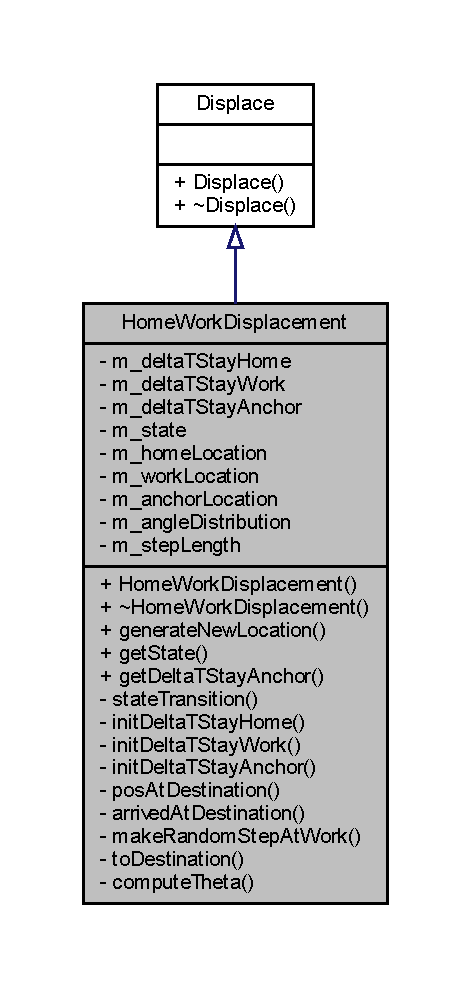
\includegraphics[width=226pt]{class_home_work_displacement__inherit__graph}
\end{center}
\end{figure}


Collaboration diagram for Home\+Work\+Displacement\+:\nopagebreak
\begin{figure}[H]
\begin{center}
\leavevmode
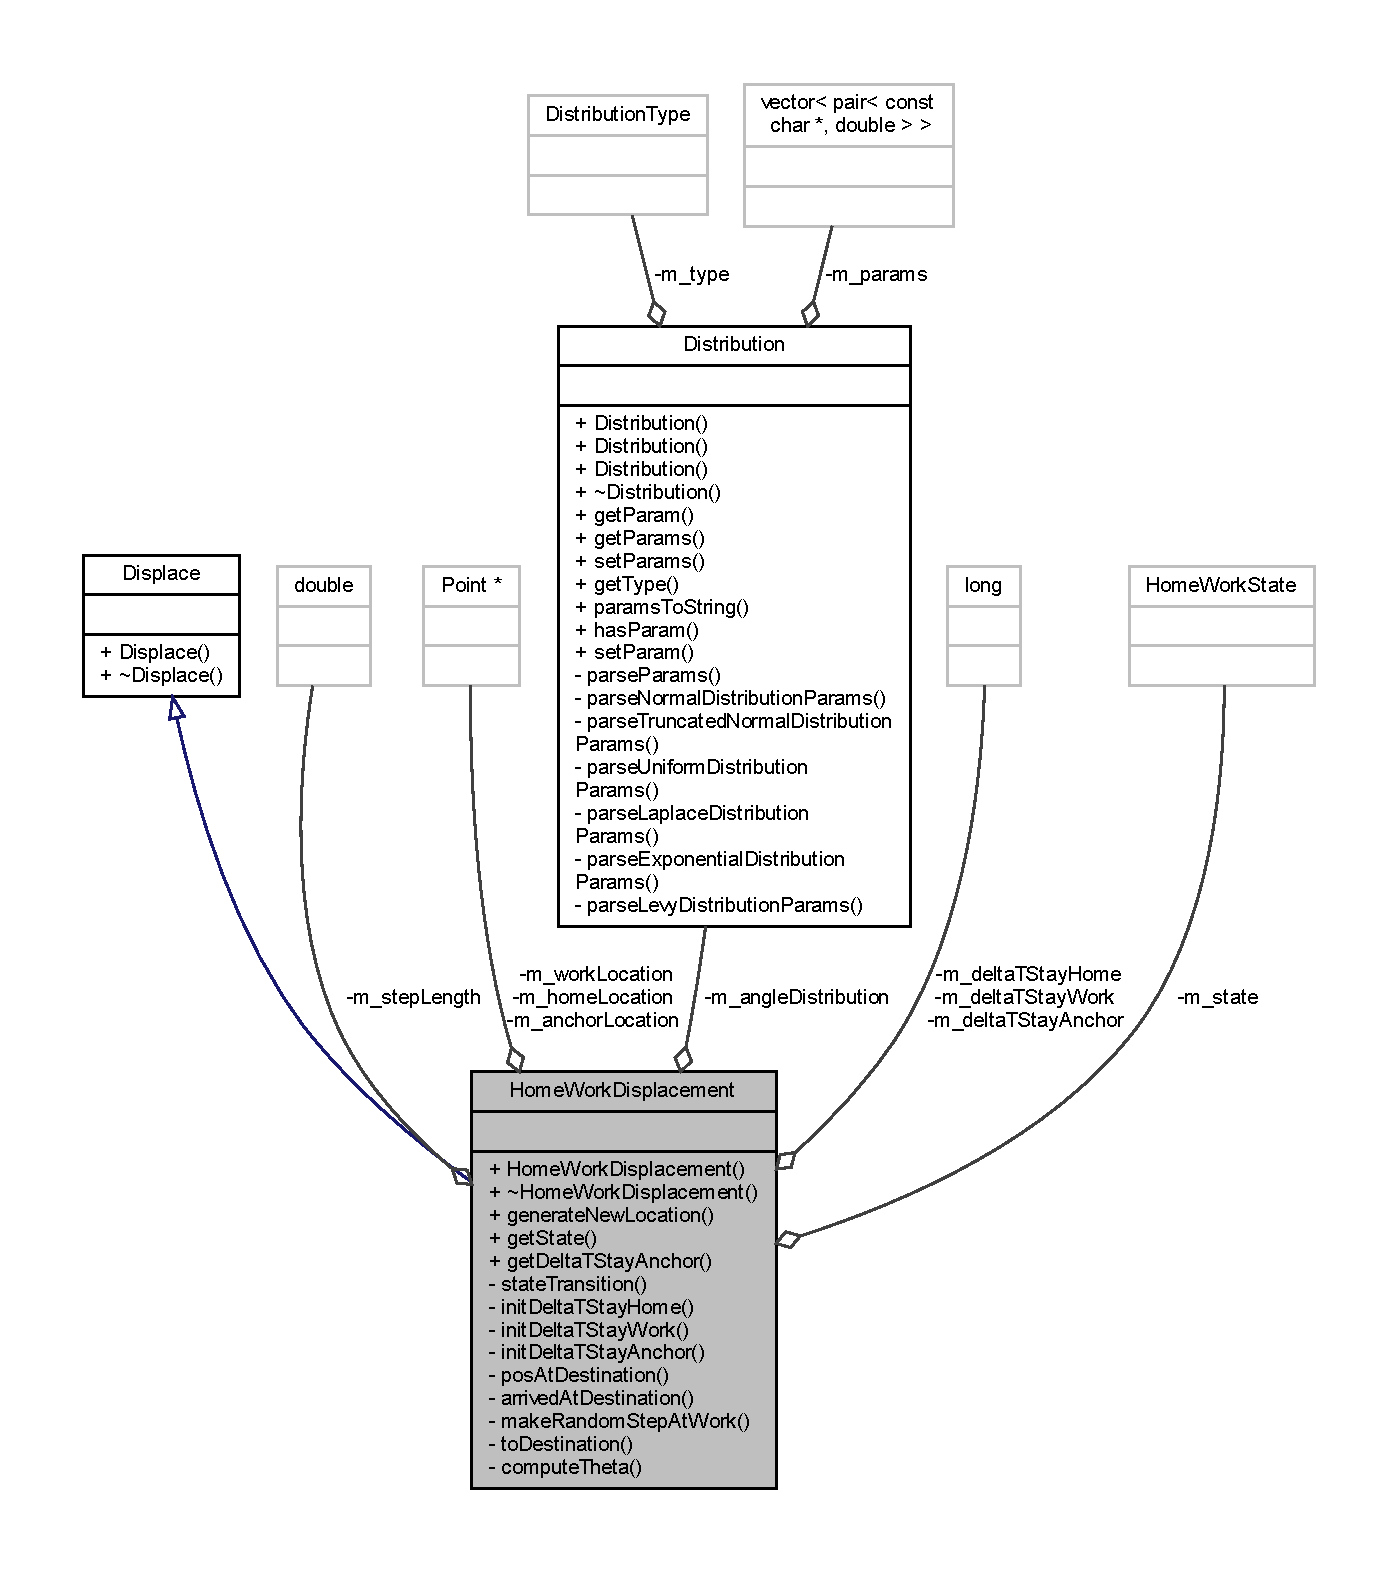
\includegraphics[width=350pt]{class_home_work_displacement__coll__graph}
\end{center}
\end{figure}
\doxysubsection*{Public Member Functions}
\begin{DoxyCompactItemize}
\item 
\mbox{\hyperlink{class_home_work_displacement_ab3ef91491bb9c4663de2b3e4735d3714}{Home\+Work\+Displacement}} (\mbox{\hyperlink{class_simulation_configuration}{Simulation\+Configuration}} $\ast$sim\+Config, double speed, Point $\ast$home\+Location, Point $\ast$work\+Location, Point $\ast$anchor\+Location)
\item 
virtual \mbox{\hyperlink{class_home_work_displacement_af47a955c24033e193c478c4271e2dbec}{$\sim$\+Home\+Work\+Displacement}} ()
\item 
virtual Point $\ast$ \mbox{\hyperlink{class_home_work_displacement_a5379a2d3450654a73104e8b0a0695a4c}{generate\+New\+Location}} (Point $\ast$p) override
\item 
\mbox{\hyperlink{_home_work_state_8h_a79c3624425f2ecf87bbc751b0194a5fe}{Home\+Work\+State}} \mbox{\hyperlink{class_home_work_displacement_a7104ff2e0ffca587c41b6995094a8e9d}{get\+State}} () const
\item 
unsigned long \mbox{\hyperlink{class_home_work_displacement_ab43675d71bcc2676c0e3522282fb82be}{get\+Delta\+T\+Stay\+Anchor}} () const
\end{DoxyCompactItemize}
\doxysubsection*{Private Member Functions}
\begin{DoxyCompactItemize}
\item 
\mbox{\hyperlink{_home_work_state_8h_a79c3624425f2ecf87bbc751b0194a5fe}{Home\+Work\+State}} \mbox{\hyperlink{class_home_work_displacement_aa1890fd829a803ec09f831e5107d5dc0}{state\+Transition}} (Point $\ast$position)
\item 
long \mbox{\hyperlink{class_home_work_displacement_a74f427c0bb25790be490e896fc245cf9}{init\+Delta\+T\+Stay\+Home}} () const
\item 
long \mbox{\hyperlink{class_home_work_displacement_a39144ce504871bcf7e9692af07c633ab}{init\+Delta\+T\+Stay\+Work}} () const
\item 
long \mbox{\hyperlink{class_home_work_displacement_a2aeacd3f9f30c5d5c4790d9db8f95fcc}{init\+Delta\+T\+Stay\+Anchor}} () const
\item 
const bool \mbox{\hyperlink{class_home_work_displacement_a6ff9dc0862bd1671241de38b23dd275a}{pos\+At\+Destination}} (Point $\ast$position, Point $\ast$destination) const
\item 
const bool \mbox{\hyperlink{class_home_work_displacement_afdaadf769b146c0c8a5be908cc1606d7}{arrived\+At\+Destination}} (Point $\ast$position, Point $\ast$destination) const
\item 
Point $\ast$ \mbox{\hyperlink{class_home_work_displacement_a8f004b1c7b587fbe80c92a3554ea20e4}{make\+Random\+Step\+At\+Work}} (Point $\ast$init\+Location)
\item 
Point $\ast$ \mbox{\hyperlink{class_home_work_displacement_a88335e3c66951079c690afe0df1e64a0}{to\+Destination}} (Point $\ast$init\+Location, Point $\ast$destination)
\item 
double \mbox{\hyperlink{class_home_work_displacement_a92e2b356a691c04368e553e780ec4672}{compute\+Theta}} (Point $\ast$p1, Point $\ast$p2) const
\end{DoxyCompactItemize}
\doxysubsection*{Private Attributes}
\begin{DoxyCompactItemize}
\item 
long \mbox{\hyperlink{class_home_work_displacement_ac8ce5bd605e720932b0b8d22e68eb690}{m\+\_\+delta\+T\+Stay\+Home}}
\item 
long \mbox{\hyperlink{class_home_work_displacement_a9924c54bac8a6fbb55c29e08c609ce43}{m\+\_\+delta\+T\+Stay\+Work}}
\item 
long \mbox{\hyperlink{class_home_work_displacement_a1fa8110be32d8a229f40f9f2228e8173}{m\+\_\+delta\+T\+Stay\+Anchor}}
\item 
\mbox{\hyperlink{_home_work_state_8h_a79c3624425f2ecf87bbc751b0194a5fe}{Home\+Work\+State}} \mbox{\hyperlink{class_home_work_displacement_a8ad94bb03504523cea98e1393d742e88}{m\+\_\+state}}
\item 
Point $\ast$ \mbox{\hyperlink{class_home_work_displacement_a57b11a4d9fef87b48105fc575ba28e42}{m\+\_\+home\+Location}}
\item 
Point $\ast$ \mbox{\hyperlink{class_home_work_displacement_aa3e7cb21c7f436f8c3f66cc4fbe565ab}{m\+\_\+work\+Location}}
\item 
Point $\ast$ \mbox{\hyperlink{class_home_work_displacement_acbd2ebba8551f709d8cb0bf28f7376a8}{m\+\_\+anchor\+Location}}
\item 
\mbox{\hyperlink{class_distribution}{Distribution}} $\ast$ \mbox{\hyperlink{class_home_work_displacement_ac3345fc1cb1b2e19eb9bc2c5df55eb06}{m\+\_\+angle\+Distribution}}
\item 
double \mbox{\hyperlink{class_home_work_displacement_ad8b747521ec921a026040fd3b6655cb8}{m\+\_\+step\+Length}}
\end{DoxyCompactItemize}


\doxysubsection{Detailed Description}
This class is part of the Strategy design pattern used to implement the displacement of persons on the map. It implements the home-\/work scenario, overriding the \mbox{\hyperlink{class_home_work_displacement_a5379a2d3450654a73104e8b0a0695a4c}{generate\+New\+Location()}} method from its superclass, \mbox{\hyperlink{class_displace}{Displace}}. 

\doxysubsection{Constructor \& Destructor Documentation}
\mbox{\Hypertarget{class_home_work_displacement_ab3ef91491bb9c4663de2b3e4735d3714}\label{class_home_work_displacement_ab3ef91491bb9c4663de2b3e4735d3714}} 
\index{HomeWorkDisplacement@{HomeWorkDisplacement}!HomeWorkDisplacement@{HomeWorkDisplacement}}
\index{HomeWorkDisplacement@{HomeWorkDisplacement}!HomeWorkDisplacement@{HomeWorkDisplacement}}
\doxysubsubsection{\texorpdfstring{HomeWorkDisplacement()}{HomeWorkDisplacement()}}
{\footnotesize\ttfamily Home\+Work\+Displacement\+::\+Home\+Work\+Displacement (\begin{DoxyParamCaption}\item[{\mbox{\hyperlink{class_simulation_configuration}{Simulation\+Configuration}} $\ast$}]{sim\+Config,  }\item[{double}]{speed,  }\item[{Point $\ast$}]{home\+Location,  }\item[{Point $\ast$}]{work\+Location,  }\item[{Point $\ast$}]{anchor\+Location }\end{DoxyParamCaption})}

This is the constructor of the class. 
\begin{DoxyParams}{Parameters}
{\em sim\+Config} & the Sim\+Config object containing the simulation configuration options read from the simulation configuration file. \\
\hline
{\em speed} & the speed of the person. This value is read from persons configuration file. \\
\hline
{\em home\+Location} & the home location. This value is set at the creation of the \mbox{\hyperlink{class_person}{Person}} object and it is a point whose coordinates are generated from a normal distribution with the parameters read from the simulation configuration file. The persons involved in a simulation are equally distributed among the home locations. \\
\hline
{\em work\+Location} & the work location the work location. This value is set at the creation of the \mbox{\hyperlink{class_person}{Person}} object and it is a point whose coordinates are generated from a normal distribution with the parameters read from the simulation configuration file. If there are several work locations in this file, a work location is assigned for each person using a uniform distribution. \\
\hline
\end{DoxyParams}
\mbox{\Hypertarget{class_home_work_displacement_af47a955c24033e193c478c4271e2dbec}\label{class_home_work_displacement_af47a955c24033e193c478c4271e2dbec}} 
\index{HomeWorkDisplacement@{HomeWorkDisplacement}!````~HomeWorkDisplacement@{$\sim$HomeWorkDisplacement}}
\index{````~HomeWorkDisplacement@{$\sim$HomeWorkDisplacement}!HomeWorkDisplacement@{HomeWorkDisplacement}}
\doxysubsubsection{\texorpdfstring{$\sim$HomeWorkDisplacement()}{~HomeWorkDisplacement()}}
{\footnotesize\ttfamily virtual Home\+Work\+Displacement\+::$\sim$\+Home\+Work\+Displacement (\begin{DoxyParamCaption}{ }\end{DoxyParamCaption})\hspace{0.3cm}{\ttfamily [virtual]}}

This is the destructor of the class. It does nothing. 

\doxysubsection{Member Function Documentation}
\mbox{\Hypertarget{class_home_work_displacement_afdaadf769b146c0c8a5be908cc1606d7}\label{class_home_work_displacement_afdaadf769b146c0c8a5be908cc1606d7}} 
\index{HomeWorkDisplacement@{HomeWorkDisplacement}!arrivedAtDestination@{arrivedAtDestination}}
\index{arrivedAtDestination@{arrivedAtDestination}!HomeWorkDisplacement@{HomeWorkDisplacement}}
\doxysubsubsection{\texorpdfstring{arrivedAtDestination()}{arrivedAtDestination()}}
{\footnotesize\ttfamily const bool Home\+Work\+Displacement\+::arrived\+At\+Destination (\begin{DoxyParamCaption}\item[{Point $\ast$}]{position,  }\item[{Point $\ast$}]{destination }\end{DoxyParamCaption}) const\hspace{0.3cm}{\ttfamily [private]}}

\mbox{\Hypertarget{class_home_work_displacement_a92e2b356a691c04368e553e780ec4672}\label{class_home_work_displacement_a92e2b356a691c04368e553e780ec4672}} 
\index{HomeWorkDisplacement@{HomeWorkDisplacement}!computeTheta@{computeTheta}}
\index{computeTheta@{computeTheta}!HomeWorkDisplacement@{HomeWorkDisplacement}}
\doxysubsubsection{\texorpdfstring{computeTheta()}{computeTheta()}}
{\footnotesize\ttfamily double Home\+Work\+Displacement\+::compute\+Theta (\begin{DoxyParamCaption}\item[{Point $\ast$}]{p1,  }\item[{Point $\ast$}]{p2 }\end{DoxyParamCaption}) const\hspace{0.3cm}{\ttfamily [private]}}

\mbox{\Hypertarget{class_home_work_displacement_a5379a2d3450654a73104e8b0a0695a4c}\label{class_home_work_displacement_a5379a2d3450654a73104e8b0a0695a4c}} 
\index{HomeWorkDisplacement@{HomeWorkDisplacement}!generateNewLocation@{generateNewLocation}}
\index{generateNewLocation@{generateNewLocation}!HomeWorkDisplacement@{HomeWorkDisplacement}}
\doxysubsubsection{\texorpdfstring{generateNewLocation()}{generateNewLocation()}}
{\footnotesize\ttfamily virtual Point$\ast$ Home\+Work\+Displacement\+::generate\+New\+Location (\begin{DoxyParamCaption}\item[{Point $\ast$}]{p }\end{DoxyParamCaption})\hspace{0.3cm}{\ttfamily [override]}, {\ttfamily [virtual]}}

Implements the home -\/ work behavior. It takes a pointer to the current location, and generates a new location according to the current status of the person. 
\begin{DoxyParams}{Parameters}
{\em p} & a pointer to the current location. \\
\hline
\end{DoxyParams}
\begin{DoxyReturn}{Returns}
the new location. 
\end{DoxyReturn}
\mbox{\Hypertarget{class_home_work_displacement_ab43675d71bcc2676c0e3522282fb82be}\label{class_home_work_displacement_ab43675d71bcc2676c0e3522282fb82be}} 
\index{HomeWorkDisplacement@{HomeWorkDisplacement}!getDeltaTStayAnchor@{getDeltaTStayAnchor}}
\index{getDeltaTStayAnchor@{getDeltaTStayAnchor}!HomeWorkDisplacement@{HomeWorkDisplacement}}
\doxysubsubsection{\texorpdfstring{getDeltaTStayAnchor()}{getDeltaTStayAnchor()}}
{\footnotesize\ttfamily unsigned long Home\+Work\+Displacement\+::get\+Delta\+T\+Stay\+Anchor (\begin{DoxyParamCaption}{ }\end{DoxyParamCaption}) const\hspace{0.3cm}{\ttfamily [inline]}}

\mbox{\Hypertarget{class_home_work_displacement_a7104ff2e0ffca587c41b6995094a8e9d}\label{class_home_work_displacement_a7104ff2e0ffca587c41b6995094a8e9d}} 
\index{HomeWorkDisplacement@{HomeWorkDisplacement}!getState@{getState}}
\index{getState@{getState}!HomeWorkDisplacement@{HomeWorkDisplacement}}
\doxysubsubsection{\texorpdfstring{getState()}{getState()}}
{\footnotesize\ttfamily \mbox{\hyperlink{_home_work_state_8h_a79c3624425f2ecf87bbc751b0194a5fe}{Home\+Work\+State}} Home\+Work\+Displacement\+::get\+State (\begin{DoxyParamCaption}{ }\end{DoxyParamCaption}) const}

\mbox{\Hypertarget{class_home_work_displacement_a2aeacd3f9f30c5d5c4790d9db8f95fcc}\label{class_home_work_displacement_a2aeacd3f9f30c5d5c4790d9db8f95fcc}} 
\index{HomeWorkDisplacement@{HomeWorkDisplacement}!initDeltaTStayAnchor@{initDeltaTStayAnchor}}
\index{initDeltaTStayAnchor@{initDeltaTStayAnchor}!HomeWorkDisplacement@{HomeWorkDisplacement}}
\doxysubsubsection{\texorpdfstring{initDeltaTStayAnchor()}{initDeltaTStayAnchor()}}
{\footnotesize\ttfamily long Home\+Work\+Displacement\+::init\+Delta\+T\+Stay\+Anchor (\begin{DoxyParamCaption}{ }\end{DoxyParamCaption}) const\hspace{0.3cm}{\ttfamily [private]}}

\mbox{\Hypertarget{class_home_work_displacement_a74f427c0bb25790be490e896fc245cf9}\label{class_home_work_displacement_a74f427c0bb25790be490e896fc245cf9}} 
\index{HomeWorkDisplacement@{HomeWorkDisplacement}!initDeltaTStayHome@{initDeltaTStayHome}}
\index{initDeltaTStayHome@{initDeltaTStayHome}!HomeWorkDisplacement@{HomeWorkDisplacement}}
\doxysubsubsection{\texorpdfstring{initDeltaTStayHome()}{initDeltaTStayHome()}}
{\footnotesize\ttfamily long Home\+Work\+Displacement\+::init\+Delta\+T\+Stay\+Home (\begin{DoxyParamCaption}{ }\end{DoxyParamCaption}) const\hspace{0.3cm}{\ttfamily [private]}}

\mbox{\Hypertarget{class_home_work_displacement_a39144ce504871bcf7e9692af07c633ab}\label{class_home_work_displacement_a39144ce504871bcf7e9692af07c633ab}} 
\index{HomeWorkDisplacement@{HomeWorkDisplacement}!initDeltaTStayWork@{initDeltaTStayWork}}
\index{initDeltaTStayWork@{initDeltaTStayWork}!HomeWorkDisplacement@{HomeWorkDisplacement}}
\doxysubsubsection{\texorpdfstring{initDeltaTStayWork()}{initDeltaTStayWork()}}
{\footnotesize\ttfamily long Home\+Work\+Displacement\+::init\+Delta\+T\+Stay\+Work (\begin{DoxyParamCaption}{ }\end{DoxyParamCaption}) const\hspace{0.3cm}{\ttfamily [private]}}

\mbox{\Hypertarget{class_home_work_displacement_a8f004b1c7b587fbe80c92a3554ea20e4}\label{class_home_work_displacement_a8f004b1c7b587fbe80c92a3554ea20e4}} 
\index{HomeWorkDisplacement@{HomeWorkDisplacement}!makeRandomStepAtWork@{makeRandomStepAtWork}}
\index{makeRandomStepAtWork@{makeRandomStepAtWork}!HomeWorkDisplacement@{HomeWorkDisplacement}}
\doxysubsubsection{\texorpdfstring{makeRandomStepAtWork()}{makeRandomStepAtWork()}}
{\footnotesize\ttfamily Point$\ast$ Home\+Work\+Displacement\+::make\+Random\+Step\+At\+Work (\begin{DoxyParamCaption}\item[{Point $\ast$}]{init\+Location }\end{DoxyParamCaption})\hspace{0.3cm}{\ttfamily [private]}}

\mbox{\Hypertarget{class_home_work_displacement_a6ff9dc0862bd1671241de38b23dd275a}\label{class_home_work_displacement_a6ff9dc0862bd1671241de38b23dd275a}} 
\index{HomeWorkDisplacement@{HomeWorkDisplacement}!posAtDestination@{posAtDestination}}
\index{posAtDestination@{posAtDestination}!HomeWorkDisplacement@{HomeWorkDisplacement}}
\doxysubsubsection{\texorpdfstring{posAtDestination()}{posAtDestination()}}
{\footnotesize\ttfamily const bool Home\+Work\+Displacement\+::pos\+At\+Destination (\begin{DoxyParamCaption}\item[{Point $\ast$}]{position,  }\item[{Point $\ast$}]{destination }\end{DoxyParamCaption}) const\hspace{0.3cm}{\ttfamily [private]}}

\mbox{\Hypertarget{class_home_work_displacement_aa1890fd829a803ec09f831e5107d5dc0}\label{class_home_work_displacement_aa1890fd829a803ec09f831e5107d5dc0}} 
\index{HomeWorkDisplacement@{HomeWorkDisplacement}!stateTransition@{stateTransition}}
\index{stateTransition@{stateTransition}!HomeWorkDisplacement@{HomeWorkDisplacement}}
\doxysubsubsection{\texorpdfstring{stateTransition()}{stateTransition()}}
{\footnotesize\ttfamily \mbox{\hyperlink{_home_work_state_8h_a79c3624425f2ecf87bbc751b0194a5fe}{Home\+Work\+State}} Home\+Work\+Displacement\+::state\+Transition (\begin{DoxyParamCaption}\item[{Point $\ast$}]{position }\end{DoxyParamCaption})\hspace{0.3cm}{\ttfamily [private]}}

\mbox{\Hypertarget{class_home_work_displacement_a88335e3c66951079c690afe0df1e64a0}\label{class_home_work_displacement_a88335e3c66951079c690afe0df1e64a0}} 
\index{HomeWorkDisplacement@{HomeWorkDisplacement}!toDestination@{toDestination}}
\index{toDestination@{toDestination}!HomeWorkDisplacement@{HomeWorkDisplacement}}
\doxysubsubsection{\texorpdfstring{toDestination()}{toDestination()}}
{\footnotesize\ttfamily Point$\ast$ Home\+Work\+Displacement\+::to\+Destination (\begin{DoxyParamCaption}\item[{Point $\ast$}]{init\+Location,  }\item[{Point $\ast$}]{destination }\end{DoxyParamCaption})\hspace{0.3cm}{\ttfamily [private]}}



\doxysubsection{Member Data Documentation}
\mbox{\Hypertarget{class_home_work_displacement_acbd2ebba8551f709d8cb0bf28f7376a8}\label{class_home_work_displacement_acbd2ebba8551f709d8cb0bf28f7376a8}} 
\index{HomeWorkDisplacement@{HomeWorkDisplacement}!m\_anchorLocation@{m\_anchorLocation}}
\index{m\_anchorLocation@{m\_anchorLocation}!HomeWorkDisplacement@{HomeWorkDisplacement}}
\doxysubsubsection{\texorpdfstring{m\_anchorLocation}{m\_anchorLocation}}
{\footnotesize\ttfamily Point$\ast$ Home\+Work\+Displacement\+::m\+\_\+anchor\+Location\hspace{0.3cm}{\ttfamily [private]}}

\mbox{\Hypertarget{class_home_work_displacement_ac3345fc1cb1b2e19eb9bc2c5df55eb06}\label{class_home_work_displacement_ac3345fc1cb1b2e19eb9bc2c5df55eb06}} 
\index{HomeWorkDisplacement@{HomeWorkDisplacement}!m\_angleDistribution@{m\_angleDistribution}}
\index{m\_angleDistribution@{m\_angleDistribution}!HomeWorkDisplacement@{HomeWorkDisplacement}}
\doxysubsubsection{\texorpdfstring{m\_angleDistribution}{m\_angleDistribution}}
{\footnotesize\ttfamily \mbox{\hyperlink{class_distribution}{Distribution}}$\ast$ Home\+Work\+Displacement\+::m\+\_\+angle\+Distribution\hspace{0.3cm}{\ttfamily [private]}}

\mbox{\Hypertarget{class_home_work_displacement_a1fa8110be32d8a229f40f9f2228e8173}\label{class_home_work_displacement_a1fa8110be32d8a229f40f9f2228e8173}} 
\index{HomeWorkDisplacement@{HomeWorkDisplacement}!m\_deltaTStayAnchor@{m\_deltaTStayAnchor}}
\index{m\_deltaTStayAnchor@{m\_deltaTStayAnchor}!HomeWorkDisplacement@{HomeWorkDisplacement}}
\doxysubsubsection{\texorpdfstring{m\_deltaTStayAnchor}{m\_deltaTStayAnchor}}
{\footnotesize\ttfamily long Home\+Work\+Displacement\+::m\+\_\+delta\+T\+Stay\+Anchor\hspace{0.3cm}{\ttfamily [private]}}

\mbox{\Hypertarget{class_home_work_displacement_ac8ce5bd605e720932b0b8d22e68eb690}\label{class_home_work_displacement_ac8ce5bd605e720932b0b8d22e68eb690}} 
\index{HomeWorkDisplacement@{HomeWorkDisplacement}!m\_deltaTStayHome@{m\_deltaTStayHome}}
\index{m\_deltaTStayHome@{m\_deltaTStayHome}!HomeWorkDisplacement@{HomeWorkDisplacement}}
\doxysubsubsection{\texorpdfstring{m\_deltaTStayHome}{m\_deltaTStayHome}}
{\footnotesize\ttfamily long Home\+Work\+Displacement\+::m\+\_\+delta\+T\+Stay\+Home\hspace{0.3cm}{\ttfamily [private]}}

\mbox{\Hypertarget{class_home_work_displacement_a9924c54bac8a6fbb55c29e08c609ce43}\label{class_home_work_displacement_a9924c54bac8a6fbb55c29e08c609ce43}} 
\index{HomeWorkDisplacement@{HomeWorkDisplacement}!m\_deltaTStayWork@{m\_deltaTStayWork}}
\index{m\_deltaTStayWork@{m\_deltaTStayWork}!HomeWorkDisplacement@{HomeWorkDisplacement}}
\doxysubsubsection{\texorpdfstring{m\_deltaTStayWork}{m\_deltaTStayWork}}
{\footnotesize\ttfamily long Home\+Work\+Displacement\+::m\+\_\+delta\+T\+Stay\+Work\hspace{0.3cm}{\ttfamily [private]}}

\mbox{\Hypertarget{class_home_work_displacement_a57b11a4d9fef87b48105fc575ba28e42}\label{class_home_work_displacement_a57b11a4d9fef87b48105fc575ba28e42}} 
\index{HomeWorkDisplacement@{HomeWorkDisplacement}!m\_homeLocation@{m\_homeLocation}}
\index{m\_homeLocation@{m\_homeLocation}!HomeWorkDisplacement@{HomeWorkDisplacement}}
\doxysubsubsection{\texorpdfstring{m\_homeLocation}{m\_homeLocation}}
{\footnotesize\ttfamily Point$\ast$ Home\+Work\+Displacement\+::m\+\_\+home\+Location\hspace{0.3cm}{\ttfamily [private]}}

\mbox{\Hypertarget{class_home_work_displacement_a8ad94bb03504523cea98e1393d742e88}\label{class_home_work_displacement_a8ad94bb03504523cea98e1393d742e88}} 
\index{HomeWorkDisplacement@{HomeWorkDisplacement}!m\_state@{m\_state}}
\index{m\_state@{m\_state}!HomeWorkDisplacement@{HomeWorkDisplacement}}
\doxysubsubsection{\texorpdfstring{m\_state}{m\_state}}
{\footnotesize\ttfamily \mbox{\hyperlink{_home_work_state_8h_a79c3624425f2ecf87bbc751b0194a5fe}{Home\+Work\+State}} Home\+Work\+Displacement\+::m\+\_\+state\hspace{0.3cm}{\ttfamily [private]}}

\mbox{\Hypertarget{class_home_work_displacement_ad8b747521ec921a026040fd3b6655cb8}\label{class_home_work_displacement_ad8b747521ec921a026040fd3b6655cb8}} 
\index{HomeWorkDisplacement@{HomeWorkDisplacement}!m\_stepLength@{m\_stepLength}}
\index{m\_stepLength@{m\_stepLength}!HomeWorkDisplacement@{HomeWorkDisplacement}}
\doxysubsubsection{\texorpdfstring{m\_stepLength}{m\_stepLength}}
{\footnotesize\ttfamily double Home\+Work\+Displacement\+::m\+\_\+step\+Length\hspace{0.3cm}{\ttfamily [private]}}

\mbox{\Hypertarget{class_home_work_displacement_aa3e7cb21c7f436f8c3f66cc4fbe565ab}\label{class_home_work_displacement_aa3e7cb21c7f436f8c3f66cc4fbe565ab}} 
\index{HomeWorkDisplacement@{HomeWorkDisplacement}!m\_workLocation@{m\_workLocation}}
\index{m\_workLocation@{m\_workLocation}!HomeWorkDisplacement@{HomeWorkDisplacement}}
\doxysubsubsection{\texorpdfstring{m\_workLocation}{m\_workLocation}}
{\footnotesize\ttfamily Point$\ast$ Home\+Work\+Displacement\+::m\+\_\+work\+Location\hspace{0.3cm}{\ttfamily [private]}}



The documentation for this class was generated from the following file\+:\begin{DoxyCompactItemize}
\item 
include/\mbox{\hyperlink{_home_work_displacement_8h}{Home\+Work\+Displacement.\+h}}\end{DoxyCompactItemize}

\hypertarget{class_home_work_location}{}\doxysection{Home\+Work\+Location Class Reference}
\label{class_home_work_location}\index{HomeWorkLocation@{HomeWorkLocation}}


{\ttfamily \#include $<$Home\+Work\+Location.\+h$>$}



Collaboration diagram for Home\+Work\+Location\+:
\nopagebreak
\begin{figure}[H]
\begin{center}
\leavevmode
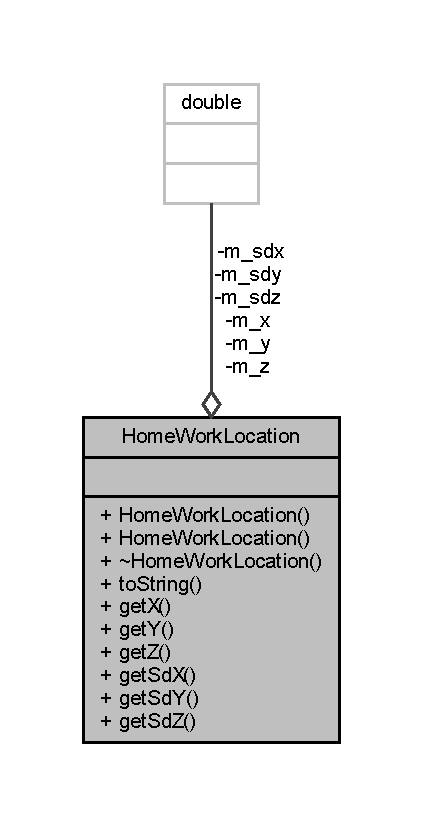
\includegraphics[width=203pt]{class_home_work_location__coll__graph}
\end{center}
\end{figure}
\doxysubsection*{Public Member Functions}
\begin{DoxyCompactItemize}
\item 
\mbox{\hyperlink{class_home_work_location_abff2c557275699910b05916c2bd884f1}{Home\+Work\+Location}} (double x, double y, double z, double sdx, double sdy, double sdz)
\item 
\mbox{\hyperlink{class_home_work_location_ae36dd03f79b906e81e2fe3b6405244d2}{Home\+Work\+Location}} ()=delete
\item 
virtual \mbox{\hyperlink{class_home_work_location_a7f8e6fa3eb2e0121fba9a35f8d665689}{$\sim$\+Home\+Work\+Location}} ()
\item 
string \mbox{\hyperlink{class_home_work_location_aa70985fa1a1601cc15be60d8762de586}{to\+String}} ()
\item 
double \mbox{\hyperlink{class_home_work_location_aea0942381f0295dc3ac1f5472311921d}{getX}} ()
\item 
double \mbox{\hyperlink{class_home_work_location_a123e4961db162c9dc176e6dfcaee760a}{getY}} ()
\item 
double \mbox{\hyperlink{class_home_work_location_a47bfccf79e9e624576f10587585d630d}{getZ}} ()
\item 
double \mbox{\hyperlink{class_home_work_location_a6461159bc4510d11886ec8405bada4b6}{get\+SdX}} ()
\item 
double \mbox{\hyperlink{class_home_work_location_adce1b4baabdaeb3a5c360a433547a162}{get\+SdY}} ()
\item 
double \mbox{\hyperlink{class_home_work_location_a51dffafd30a47607b2101567f9af71a3}{get\+SdZ}} ()
\end{DoxyCompactItemize}
\doxysubsection*{Private Attributes}
\begin{DoxyCompactItemize}
\item 
double \mbox{\hyperlink{class_home_work_location_a174434e751725e45a3b504399d02a86a}{m\+\_\+x}}
\item 
double \mbox{\hyperlink{class_home_work_location_aff6ad4ce0e02e5cbc04df0b569c70628}{m\+\_\+y}}
\item 
double \mbox{\hyperlink{class_home_work_location_aaa9a349f69741eb2a7acacbcbe99d234}{m\+\_\+z}}
\item 
double \mbox{\hyperlink{class_home_work_location_abffab0815318cb942ca957481777bae9}{m\+\_\+sdx}}
\item 
double \mbox{\hyperlink{class_home_work_location_aeb2723b99f348b9d3c208da8e48547ba}{m\+\_\+sdy}}
\item 
double \mbox{\hyperlink{class_home_work_location_ad1bf94d5b6415f4d598dfbd92eb00d82}{m\+\_\+sdz}}
\end{DoxyCompactItemize}


\doxysubsection{Detailed Description}
This class encapsulates the information needed to generate the home or work location on the map. All the information need to build a \mbox{\hyperlink{class_home_work_location}{Home\+Work\+Location}} object are read from the simulation configuration file. 

\doxysubsection{Constructor \& Destructor Documentation}
\mbox{\Hypertarget{class_home_work_location_abff2c557275699910b05916c2bd884f1}\label{class_home_work_location_abff2c557275699910b05916c2bd884f1}} 
\index{HomeWorkLocation@{HomeWorkLocation}!HomeWorkLocation@{HomeWorkLocation}}
\index{HomeWorkLocation@{HomeWorkLocation}!HomeWorkLocation@{HomeWorkLocation}}
\doxysubsubsection{\texorpdfstring{HomeWorkLocation()}{HomeWorkLocation()}\hspace{0.1cm}{\footnotesize\ttfamily [1/2]}}
{\footnotesize\ttfamily Home\+Work\+Location\+::\+Home\+Work\+Location (\begin{DoxyParamCaption}\item[{double}]{x,  }\item[{double}]{y,  }\item[{double}]{z,  }\item[{double}]{sdx,  }\item[{double}]{sdy,  }\item[{double}]{sdz }\end{DoxyParamCaption})}

Constructor of the class. It builds a \mbox{\hyperlink{class_home_work_location}{Home\+Work\+Location}} object by setting its members using the values passed as parameters. 
\begin{DoxyParams}{Parameters}
{\em x} & the x coordinate of a Home -\/ Work location. \\
\hline
{\em y} & the y coordinate of a Home -\/ Work location. \\
\hline
{\em z} & the z coordinate of a Home -\/ Work location. \\
\hline
{\em sdx} & the standard deviation / radius of the x coordinate of a Home -\/ Work location. \\
\hline
{\em sdy} & the standard deviation / radius of the y coordinate of a Home -\/ Work location. \\
\hline
{\em sdz} & the standard deviation / radius of the z coordinate of a Home -\/ Work location. \\
\hline
\end{DoxyParams}
\mbox{\Hypertarget{class_home_work_location_ae36dd03f79b906e81e2fe3b6405244d2}\label{class_home_work_location_ae36dd03f79b906e81e2fe3b6405244d2}} 
\index{HomeWorkLocation@{HomeWorkLocation}!HomeWorkLocation@{HomeWorkLocation}}
\index{HomeWorkLocation@{HomeWorkLocation}!HomeWorkLocation@{HomeWorkLocation}}
\doxysubsubsection{\texorpdfstring{HomeWorkLocation()}{HomeWorkLocation()}\hspace{0.1cm}{\footnotesize\ttfamily [2/2]}}
{\footnotesize\ttfamily Home\+Work\+Location\+::\+Home\+Work\+Location (\begin{DoxyParamCaption}{ }\end{DoxyParamCaption})\hspace{0.3cm}{\ttfamily [delete]}}

The default constructor is deleted. A \mbox{\hyperlink{class_home_work_location}{Home\+Work\+Location}} object without the values for the members makes no sense. \mbox{\Hypertarget{class_home_work_location_a7f8e6fa3eb2e0121fba9a35f8d665689}\label{class_home_work_location_a7f8e6fa3eb2e0121fba9a35f8d665689}} 
\index{HomeWorkLocation@{HomeWorkLocation}!````~HomeWorkLocation@{$\sim$HomeWorkLocation}}
\index{````~HomeWorkLocation@{$\sim$HomeWorkLocation}!HomeWorkLocation@{HomeWorkLocation}}
\doxysubsubsection{\texorpdfstring{$\sim$HomeWorkLocation()}{~HomeWorkLocation()}}
{\footnotesize\ttfamily virtual Home\+Work\+Location\+::$\sim$\+Home\+Work\+Location (\begin{DoxyParamCaption}{ }\end{DoxyParamCaption})\hspace{0.3cm}{\ttfamily [virtual]}}

Default destructor. 

\doxysubsection{Member Function Documentation}
\mbox{\Hypertarget{class_home_work_location_a6461159bc4510d11886ec8405bada4b6}\label{class_home_work_location_a6461159bc4510d11886ec8405bada4b6}} 
\index{HomeWorkLocation@{HomeWorkLocation}!getSdX@{getSdX}}
\index{getSdX@{getSdX}!HomeWorkLocation@{HomeWorkLocation}}
\doxysubsubsection{\texorpdfstring{getSdX()}{getSdX()}}
{\footnotesize\ttfamily double Home\+Work\+Location\+::get\+SdX (\begin{DoxyParamCaption}{ }\end{DoxyParamCaption})\hspace{0.3cm}{\ttfamily [inline]}}

\begin{DoxyReturn}{Returns}

\end{DoxyReturn}
\mbox{\Hypertarget{class_home_work_location_adce1b4baabdaeb3a5c360a433547a162}\label{class_home_work_location_adce1b4baabdaeb3a5c360a433547a162}} 
\index{HomeWorkLocation@{HomeWorkLocation}!getSdY@{getSdY}}
\index{getSdY@{getSdY}!HomeWorkLocation@{HomeWorkLocation}}
\doxysubsubsection{\texorpdfstring{getSdY()}{getSdY()}}
{\footnotesize\ttfamily double Home\+Work\+Location\+::get\+SdY (\begin{DoxyParamCaption}{ }\end{DoxyParamCaption})\hspace{0.3cm}{\ttfamily [inline]}}

\begin{DoxyReturn}{Returns}

\end{DoxyReturn}
\mbox{\Hypertarget{class_home_work_location_a51dffafd30a47607b2101567f9af71a3}\label{class_home_work_location_a51dffafd30a47607b2101567f9af71a3}} 
\index{HomeWorkLocation@{HomeWorkLocation}!getSdZ@{getSdZ}}
\index{getSdZ@{getSdZ}!HomeWorkLocation@{HomeWorkLocation}}
\doxysubsubsection{\texorpdfstring{getSdZ()}{getSdZ()}}
{\footnotesize\ttfamily double Home\+Work\+Location\+::get\+SdZ (\begin{DoxyParamCaption}{ }\end{DoxyParamCaption})\hspace{0.3cm}{\ttfamily [inline]}}

\begin{DoxyReturn}{Returns}

\end{DoxyReturn}
\mbox{\Hypertarget{class_home_work_location_aea0942381f0295dc3ac1f5472311921d}\label{class_home_work_location_aea0942381f0295dc3ac1f5472311921d}} 
\index{HomeWorkLocation@{HomeWorkLocation}!getX@{getX}}
\index{getX@{getX}!HomeWorkLocation@{HomeWorkLocation}}
\doxysubsubsection{\texorpdfstring{getX()}{getX()}}
{\footnotesize\ttfamily double Home\+Work\+Location\+::getX (\begin{DoxyParamCaption}{ }\end{DoxyParamCaption})\hspace{0.3cm}{\ttfamily [inline]}}

\begin{DoxyReturn}{Returns}

\end{DoxyReturn}
\mbox{\Hypertarget{class_home_work_location_a123e4961db162c9dc176e6dfcaee760a}\label{class_home_work_location_a123e4961db162c9dc176e6dfcaee760a}} 
\index{HomeWorkLocation@{HomeWorkLocation}!getY@{getY}}
\index{getY@{getY}!HomeWorkLocation@{HomeWorkLocation}}
\doxysubsubsection{\texorpdfstring{getY()}{getY()}}
{\footnotesize\ttfamily double Home\+Work\+Location\+::getY (\begin{DoxyParamCaption}{ }\end{DoxyParamCaption})\hspace{0.3cm}{\ttfamily [inline]}}

\begin{DoxyReturn}{Returns}

\end{DoxyReturn}
\mbox{\Hypertarget{class_home_work_location_a47bfccf79e9e624576f10587585d630d}\label{class_home_work_location_a47bfccf79e9e624576f10587585d630d}} 
\index{HomeWorkLocation@{HomeWorkLocation}!getZ@{getZ}}
\index{getZ@{getZ}!HomeWorkLocation@{HomeWorkLocation}}
\doxysubsubsection{\texorpdfstring{getZ()}{getZ()}}
{\footnotesize\ttfamily double Home\+Work\+Location\+::getZ (\begin{DoxyParamCaption}{ }\end{DoxyParamCaption})\hspace{0.3cm}{\ttfamily [inline]}}

\begin{DoxyReturn}{Returns}

\end{DoxyReturn}
\mbox{\Hypertarget{class_home_work_location_aa70985fa1a1601cc15be60d8762de586}\label{class_home_work_location_aa70985fa1a1601cc15be60d8762de586}} 
\index{HomeWorkLocation@{HomeWorkLocation}!toString@{toString}}
\index{toString@{toString}!HomeWorkLocation@{HomeWorkLocation}}
\doxysubsubsection{\texorpdfstring{toString()}{toString()}}
{\footnotesize\ttfamily string Home\+Work\+Location\+::to\+String (\begin{DoxyParamCaption}{ }\end{DoxyParamCaption})}

Return a string representation of the class, containing the values of all members, comma separated. It is useful for debugging or for printing these information. An example of such a string\+:


\begin{DoxyCode}{0}
\DoxyCodeLine{X:2000 Y:7500 Z:0 Sd\_x:1000 Sd\_y:1000 Sd\_z:0}
\end{DoxyCode}


\begin{DoxyReturn}{Returns}
a string representation of the class, containing the values of all members, comma separated. 
\end{DoxyReturn}


\doxysubsection{Member Data Documentation}
\mbox{\Hypertarget{class_home_work_location_abffab0815318cb942ca957481777bae9}\label{class_home_work_location_abffab0815318cb942ca957481777bae9}} 
\index{HomeWorkLocation@{HomeWorkLocation}!m\_sdx@{m\_sdx}}
\index{m\_sdx@{m\_sdx}!HomeWorkLocation@{HomeWorkLocation}}
\doxysubsubsection{\texorpdfstring{m\_sdx}{m\_sdx}}
{\footnotesize\ttfamily double Home\+Work\+Location\+::m\+\_\+sdx\hspace{0.3cm}{\ttfamily [private]}}

\mbox{\Hypertarget{class_home_work_location_aeb2723b99f348b9d3c208da8e48547ba}\label{class_home_work_location_aeb2723b99f348b9d3c208da8e48547ba}} 
\index{HomeWorkLocation@{HomeWorkLocation}!m\_sdy@{m\_sdy}}
\index{m\_sdy@{m\_sdy}!HomeWorkLocation@{HomeWorkLocation}}
\doxysubsubsection{\texorpdfstring{m\_sdy}{m\_sdy}}
{\footnotesize\ttfamily double Home\+Work\+Location\+::m\+\_\+sdy\hspace{0.3cm}{\ttfamily [private]}}

\mbox{\Hypertarget{class_home_work_location_ad1bf94d5b6415f4d598dfbd92eb00d82}\label{class_home_work_location_ad1bf94d5b6415f4d598dfbd92eb00d82}} 
\index{HomeWorkLocation@{HomeWorkLocation}!m\_sdz@{m\_sdz}}
\index{m\_sdz@{m\_sdz}!HomeWorkLocation@{HomeWorkLocation}}
\doxysubsubsection{\texorpdfstring{m\_sdz}{m\_sdz}}
{\footnotesize\ttfamily double Home\+Work\+Location\+::m\+\_\+sdz\hspace{0.3cm}{\ttfamily [private]}}

\mbox{\Hypertarget{class_home_work_location_a174434e751725e45a3b504399d02a86a}\label{class_home_work_location_a174434e751725e45a3b504399d02a86a}} 
\index{HomeWorkLocation@{HomeWorkLocation}!m\_x@{m\_x}}
\index{m\_x@{m\_x}!HomeWorkLocation@{HomeWorkLocation}}
\doxysubsubsection{\texorpdfstring{m\_x}{m\_x}}
{\footnotesize\ttfamily double Home\+Work\+Location\+::m\+\_\+x\hspace{0.3cm}{\ttfamily [private]}}

\mbox{\Hypertarget{class_home_work_location_aff6ad4ce0e02e5cbc04df0b569c70628}\label{class_home_work_location_aff6ad4ce0e02e5cbc04df0b569c70628}} 
\index{HomeWorkLocation@{HomeWorkLocation}!m\_y@{m\_y}}
\index{m\_y@{m\_y}!HomeWorkLocation@{HomeWorkLocation}}
\doxysubsubsection{\texorpdfstring{m\_y}{m\_y}}
{\footnotesize\ttfamily double Home\+Work\+Location\+::m\+\_\+y\hspace{0.3cm}{\ttfamily [private]}}

\mbox{\Hypertarget{class_home_work_location_aaa9a349f69741eb2a7acacbcbe99d234}\label{class_home_work_location_aaa9a349f69741eb2a7acacbcbe99d234}} 
\index{HomeWorkLocation@{HomeWorkLocation}!m\_z@{m\_z}}
\index{m\_z@{m\_z}!HomeWorkLocation@{HomeWorkLocation}}
\doxysubsubsection{\texorpdfstring{m\_z}{m\_z}}
{\footnotesize\ttfamily double Home\+Work\+Location\+::m\+\_\+z\hspace{0.3cm}{\ttfamily [private]}}



The documentation for this class was generated from the following file\+:\begin{DoxyCompactItemize}
\item 
include/parsers/\mbox{\hyperlink{_home_work_location_8h}{Home\+Work\+Location.\+h}}\end{DoxyCompactItemize}

\hypertarget{class_home_work_scenario}{}\doxysection{Home\+Work\+Scenario Class Reference}
\label{class_home_work_scenario}\index{HomeWorkScenario@{HomeWorkScenario}}


{\ttfamily \#include $<$Home\+Work\+Scenario.\+h$>$}



Collaboration diagram for Home\+Work\+Scenario\+:\nopagebreak
\begin{figure}[H]
\begin{center}
\leavevmode
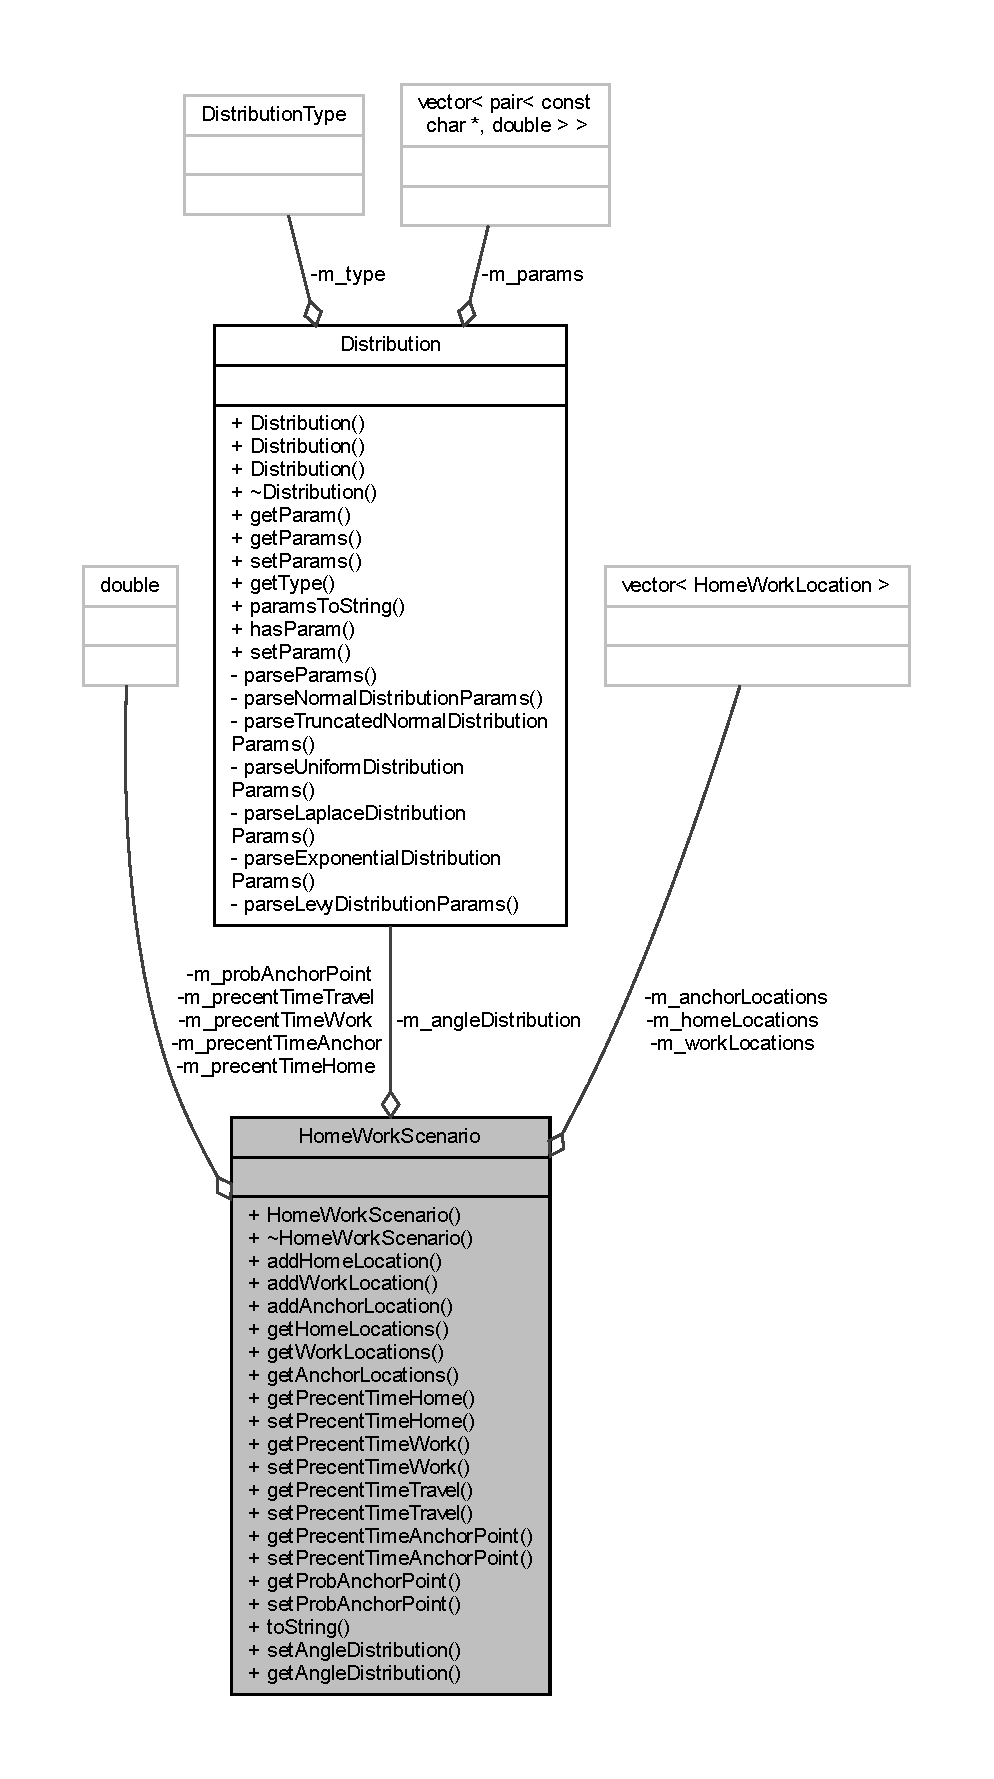
\includegraphics[height=550pt]{class_home_work_scenario__coll__graph}
\end{center}
\end{figure}
\doxysubsection*{Public Member Functions}
\begin{DoxyCompactItemize}
\item 
\mbox{\hyperlink{class_home_work_scenario_a9401be1318be8a3cc2484e4f47dd8937}{Home\+Work\+Scenario}} ()
\item 
virtual \mbox{\hyperlink{class_home_work_scenario_ada2d075a585e9e258642d486b1087cc1}{$\sim$\+Home\+Work\+Scenario}} ()
\item 
void \mbox{\hyperlink{class_home_work_scenario_a161ff2fc62e20284bd74260b0e55508b}{add\+Home\+Location}} (\mbox{\hyperlink{class_home_work_location}{Home\+Work\+Location}} h)
\item 
void \mbox{\hyperlink{class_home_work_scenario_a4dac1088a1702823cdfd210f262f09da}{add\+Work\+Location}} (\mbox{\hyperlink{class_home_work_location}{Home\+Work\+Location}} h)
\item 
void \mbox{\hyperlink{class_home_work_scenario_ae4bc8100869e3ff8ded3c1404c38b678}{add\+Anchor\+Location}} (\mbox{\hyperlink{class_home_work_location}{Home\+Work\+Location}} h)
\item 
vector$<$ \mbox{\hyperlink{class_home_work_location}{Home\+Work\+Location}} $>$ \mbox{\hyperlink{class_home_work_scenario_acfeaf7a6e25c64cac62a9776cf8bb341}{get\+Home\+Locations}} () const
\item 
vector$<$ \mbox{\hyperlink{class_home_work_location}{Home\+Work\+Location}} $>$ \mbox{\hyperlink{class_home_work_scenario_abc93a27b7d5e438ad377e6380889094e}{get\+Work\+Locations}} () const
\item 
vector$<$ \mbox{\hyperlink{class_home_work_location}{Home\+Work\+Location}} $>$ \mbox{\hyperlink{class_home_work_scenario_a3a7f3011fa1f5ed0ff5b5056faab8115}{get\+Anchor\+Locations}} () const
\item 
double \mbox{\hyperlink{class_home_work_scenario_a6e99d6ec212721d6b542e06aca768c97}{get\+Precent\+Time\+Home}} () const
\item 
void \mbox{\hyperlink{class_home_work_scenario_add355d82806b3c32c1da9ae5360937d4}{set\+Precent\+Time\+Home}} (double precent\+Time\+Home)
\item 
double \mbox{\hyperlink{class_home_work_scenario_adfa68f72b123bf36f8aa97a986f08565}{get\+Precent\+Time\+Work}} () const
\item 
void \mbox{\hyperlink{class_home_work_scenario_ac287b0faaae42cd917a06e1dd9b49f69}{set\+Precent\+Time\+Work}} (double precent\+Time\+Work)
\item 
double \mbox{\hyperlink{class_home_work_scenario_aa4c6f4ce09a2f38a62e787c60e1dec6b}{get\+Precent\+Time\+Travel}} () const
\item 
void \mbox{\hyperlink{class_home_work_scenario_a7d7fc398d7748e915370dc08417d2d85}{set\+Precent\+Time\+Travel}} (double precent\+Timetravel)
\item 
double \mbox{\hyperlink{class_home_work_scenario_a420d76c8e88f762833744680407d3265}{get\+Precent\+Time\+Anchor\+Point}} () const
\item 
void \mbox{\hyperlink{class_home_work_scenario_a0acbf37eb6ab3c09c4092ccc481f1497}{set\+Precent\+Time\+Anchor\+Point}} (double precent\+Time\+Anchor)
\item 
double \mbox{\hyperlink{class_home_work_scenario_aa3ecc23cfe53510130073d8abe96b434}{get\+Prob\+Anchor\+Point}} () const
\item 
void \mbox{\hyperlink{class_home_work_scenario_afb2d2cfcdd225c95da44e642f907f8bc}{set\+Prob\+Anchor\+Point}} (double precent\+Time\+Anchor)
\item 
const string \mbox{\hyperlink{class_home_work_scenario_a099fe2cf41a05087752efb96a3c8f068}{to\+String}} ()
\item 
void \mbox{\hyperlink{class_home_work_scenario_a900316b0eebefa3d1190190627593c35}{set\+Angle\+Distribution}} (\mbox{\hyperlink{class_distribution}{Distribution}} $\ast$distr)
\item 
\mbox{\hyperlink{class_distribution}{Distribution}} $\ast$ \mbox{\hyperlink{class_home_work_scenario_a45fe6d50574b00a8ea6d895d667d275b}{get\+Angle\+Distribution}} ()
\end{DoxyCompactItemize}
\doxysubsection*{Private Attributes}
\begin{DoxyCompactItemize}
\item 
vector$<$ \mbox{\hyperlink{class_home_work_location}{Home\+Work\+Location}} $>$ \mbox{\hyperlink{class_home_work_scenario_a9996ae2074dcce49ed9ee8d8a90c8dc6}{m\+\_\+home\+Locations}}
\item 
vector$<$ \mbox{\hyperlink{class_home_work_location}{Home\+Work\+Location}} $>$ \mbox{\hyperlink{class_home_work_scenario_a0a04c40ac3f3a4723499d275b415fbf0}{m\+\_\+work\+Locations}}
\item 
vector$<$ \mbox{\hyperlink{class_home_work_location}{Home\+Work\+Location}} $>$ \mbox{\hyperlink{class_home_work_scenario_a6efe837def2eb5a74f536bdf42eedfd9}{m\+\_\+anchor\+Locations}}
\item 
double \mbox{\hyperlink{class_home_work_scenario_adb5d68236b7b8719b82170a02ee257e2}{m\+\_\+precent\+Time\+Home}}
\item 
double \mbox{\hyperlink{class_home_work_scenario_a5ac962b01265541ac5dea2b622e52caf}{m\+\_\+precent\+Time\+Work}}
\item 
double \mbox{\hyperlink{class_home_work_scenario_a9806633ba24978407f8e7d248e49cee6}{m\+\_\+precent\+Time\+Anchor}}
\item 
double \mbox{\hyperlink{class_home_work_scenario_aa051d3cbf714fdeba83982c1cb0b6962}{m\+\_\+precent\+Time\+Travel}}
\item 
double \mbox{\hyperlink{class_home_work_scenario_a34a02f9267f5006190cedd251bb4b00f}{m\+\_\+prob\+Anchor\+Point}}
\item 
\mbox{\hyperlink{class_distribution}{Distribution}} $\ast$ \mbox{\hyperlink{class_home_work_scenario_a8181bf6ba705970683baa6d57151fa39}{m\+\_\+angle\+Distribution}}
\end{DoxyCompactItemize}


\doxysubsection{Constructor \& Destructor Documentation}
\mbox{\Hypertarget{class_home_work_scenario_a9401be1318be8a3cc2484e4f47dd8937}\label{class_home_work_scenario_a9401be1318be8a3cc2484e4f47dd8937}} 
\index{HomeWorkScenario@{HomeWorkScenario}!HomeWorkScenario@{HomeWorkScenario}}
\index{HomeWorkScenario@{HomeWorkScenario}!HomeWorkScenario@{HomeWorkScenario}}
\doxysubsubsection{\texorpdfstring{HomeWorkScenario()}{HomeWorkScenario()}}
{\footnotesize\ttfamily Home\+Work\+Scenario\+::\+Home\+Work\+Scenario (\begin{DoxyParamCaption}{ }\end{DoxyParamCaption})}

\mbox{\Hypertarget{class_home_work_scenario_ada2d075a585e9e258642d486b1087cc1}\label{class_home_work_scenario_ada2d075a585e9e258642d486b1087cc1}} 
\index{HomeWorkScenario@{HomeWorkScenario}!````~HomeWorkScenario@{$\sim$HomeWorkScenario}}
\index{````~HomeWorkScenario@{$\sim$HomeWorkScenario}!HomeWorkScenario@{HomeWorkScenario}}
\doxysubsubsection{\texorpdfstring{$\sim$HomeWorkScenario()}{~HomeWorkScenario()}}
{\footnotesize\ttfamily virtual Home\+Work\+Scenario\+::$\sim$\+Home\+Work\+Scenario (\begin{DoxyParamCaption}{ }\end{DoxyParamCaption})\hspace{0.3cm}{\ttfamily [virtual]}}



\doxysubsection{Member Function Documentation}
\mbox{\Hypertarget{class_home_work_scenario_ae4bc8100869e3ff8ded3c1404c38b678}\label{class_home_work_scenario_ae4bc8100869e3ff8ded3c1404c38b678}} 
\index{HomeWorkScenario@{HomeWorkScenario}!addAnchorLocation@{addAnchorLocation}}
\index{addAnchorLocation@{addAnchorLocation}!HomeWorkScenario@{HomeWorkScenario}}
\doxysubsubsection{\texorpdfstring{addAnchorLocation()}{addAnchorLocation()}}
{\footnotesize\ttfamily void Home\+Work\+Scenario\+::add\+Anchor\+Location (\begin{DoxyParamCaption}\item[{\mbox{\hyperlink{class_home_work_location}{Home\+Work\+Location}}}]{h }\end{DoxyParamCaption})}

\mbox{\Hypertarget{class_home_work_scenario_a161ff2fc62e20284bd74260b0e55508b}\label{class_home_work_scenario_a161ff2fc62e20284bd74260b0e55508b}} 
\index{HomeWorkScenario@{HomeWorkScenario}!addHomeLocation@{addHomeLocation}}
\index{addHomeLocation@{addHomeLocation}!HomeWorkScenario@{HomeWorkScenario}}
\doxysubsubsection{\texorpdfstring{addHomeLocation()}{addHomeLocation()}}
{\footnotesize\ttfamily void Home\+Work\+Scenario\+::add\+Home\+Location (\begin{DoxyParamCaption}\item[{\mbox{\hyperlink{class_home_work_location}{Home\+Work\+Location}}}]{h }\end{DoxyParamCaption})}

\mbox{\Hypertarget{class_home_work_scenario_a4dac1088a1702823cdfd210f262f09da}\label{class_home_work_scenario_a4dac1088a1702823cdfd210f262f09da}} 
\index{HomeWorkScenario@{HomeWorkScenario}!addWorkLocation@{addWorkLocation}}
\index{addWorkLocation@{addWorkLocation}!HomeWorkScenario@{HomeWorkScenario}}
\doxysubsubsection{\texorpdfstring{addWorkLocation()}{addWorkLocation()}}
{\footnotesize\ttfamily void Home\+Work\+Scenario\+::add\+Work\+Location (\begin{DoxyParamCaption}\item[{\mbox{\hyperlink{class_home_work_location}{Home\+Work\+Location}}}]{h }\end{DoxyParamCaption})}

\mbox{\Hypertarget{class_home_work_scenario_a3a7f3011fa1f5ed0ff5b5056faab8115}\label{class_home_work_scenario_a3a7f3011fa1f5ed0ff5b5056faab8115}} 
\index{HomeWorkScenario@{HomeWorkScenario}!getAnchorLocations@{getAnchorLocations}}
\index{getAnchorLocations@{getAnchorLocations}!HomeWorkScenario@{HomeWorkScenario}}
\doxysubsubsection{\texorpdfstring{getAnchorLocations()}{getAnchorLocations()}}
{\footnotesize\ttfamily vector$<$\mbox{\hyperlink{class_home_work_location}{Home\+Work\+Location}}$>$ Home\+Work\+Scenario\+::get\+Anchor\+Locations (\begin{DoxyParamCaption}{ }\end{DoxyParamCaption}) const}

\mbox{\Hypertarget{class_home_work_scenario_a45fe6d50574b00a8ea6d895d667d275b}\label{class_home_work_scenario_a45fe6d50574b00a8ea6d895d667d275b}} 
\index{HomeWorkScenario@{HomeWorkScenario}!getAngleDistribution@{getAngleDistribution}}
\index{getAngleDistribution@{getAngleDistribution}!HomeWorkScenario@{HomeWorkScenario}}
\doxysubsubsection{\texorpdfstring{getAngleDistribution()}{getAngleDistribution()}}
{\footnotesize\ttfamily \mbox{\hyperlink{class_distribution}{Distribution}}$\ast$ Home\+Work\+Scenario\+::get\+Angle\+Distribution (\begin{DoxyParamCaption}{ }\end{DoxyParamCaption})}

\mbox{\Hypertarget{class_home_work_scenario_acfeaf7a6e25c64cac62a9776cf8bb341}\label{class_home_work_scenario_acfeaf7a6e25c64cac62a9776cf8bb341}} 
\index{HomeWorkScenario@{HomeWorkScenario}!getHomeLocations@{getHomeLocations}}
\index{getHomeLocations@{getHomeLocations}!HomeWorkScenario@{HomeWorkScenario}}
\doxysubsubsection{\texorpdfstring{getHomeLocations()}{getHomeLocations()}}
{\footnotesize\ttfamily vector$<$\mbox{\hyperlink{class_home_work_location}{Home\+Work\+Location}}$>$ Home\+Work\+Scenario\+::get\+Home\+Locations (\begin{DoxyParamCaption}{ }\end{DoxyParamCaption}) const}

\mbox{\Hypertarget{class_home_work_scenario_a420d76c8e88f762833744680407d3265}\label{class_home_work_scenario_a420d76c8e88f762833744680407d3265}} 
\index{HomeWorkScenario@{HomeWorkScenario}!getPrecentTimeAnchorPoint@{getPrecentTimeAnchorPoint}}
\index{getPrecentTimeAnchorPoint@{getPrecentTimeAnchorPoint}!HomeWorkScenario@{HomeWorkScenario}}
\doxysubsubsection{\texorpdfstring{getPrecentTimeAnchorPoint()}{getPrecentTimeAnchorPoint()}}
{\footnotesize\ttfamily double Home\+Work\+Scenario\+::get\+Precent\+Time\+Anchor\+Point (\begin{DoxyParamCaption}{ }\end{DoxyParamCaption}) const}

\mbox{\Hypertarget{class_home_work_scenario_a6e99d6ec212721d6b542e06aca768c97}\label{class_home_work_scenario_a6e99d6ec212721d6b542e06aca768c97}} 
\index{HomeWorkScenario@{HomeWorkScenario}!getPrecentTimeHome@{getPrecentTimeHome}}
\index{getPrecentTimeHome@{getPrecentTimeHome}!HomeWorkScenario@{HomeWorkScenario}}
\doxysubsubsection{\texorpdfstring{getPrecentTimeHome()}{getPrecentTimeHome()}}
{\footnotesize\ttfamily double Home\+Work\+Scenario\+::get\+Precent\+Time\+Home (\begin{DoxyParamCaption}{ }\end{DoxyParamCaption}) const}

\mbox{\Hypertarget{class_home_work_scenario_aa4c6f4ce09a2f38a62e787c60e1dec6b}\label{class_home_work_scenario_aa4c6f4ce09a2f38a62e787c60e1dec6b}} 
\index{HomeWorkScenario@{HomeWorkScenario}!getPrecentTimeTravel@{getPrecentTimeTravel}}
\index{getPrecentTimeTravel@{getPrecentTimeTravel}!HomeWorkScenario@{HomeWorkScenario}}
\doxysubsubsection{\texorpdfstring{getPrecentTimeTravel()}{getPrecentTimeTravel()}}
{\footnotesize\ttfamily double Home\+Work\+Scenario\+::get\+Precent\+Time\+Travel (\begin{DoxyParamCaption}{ }\end{DoxyParamCaption}) const}

\mbox{\Hypertarget{class_home_work_scenario_adfa68f72b123bf36f8aa97a986f08565}\label{class_home_work_scenario_adfa68f72b123bf36f8aa97a986f08565}} 
\index{HomeWorkScenario@{HomeWorkScenario}!getPrecentTimeWork@{getPrecentTimeWork}}
\index{getPrecentTimeWork@{getPrecentTimeWork}!HomeWorkScenario@{HomeWorkScenario}}
\doxysubsubsection{\texorpdfstring{getPrecentTimeWork()}{getPrecentTimeWork()}}
{\footnotesize\ttfamily double Home\+Work\+Scenario\+::get\+Precent\+Time\+Work (\begin{DoxyParamCaption}{ }\end{DoxyParamCaption}) const}

\mbox{\Hypertarget{class_home_work_scenario_aa3ecc23cfe53510130073d8abe96b434}\label{class_home_work_scenario_aa3ecc23cfe53510130073d8abe96b434}} 
\index{HomeWorkScenario@{HomeWorkScenario}!getProbAnchorPoint@{getProbAnchorPoint}}
\index{getProbAnchorPoint@{getProbAnchorPoint}!HomeWorkScenario@{HomeWorkScenario}}
\doxysubsubsection{\texorpdfstring{getProbAnchorPoint()}{getProbAnchorPoint()}}
{\footnotesize\ttfamily double Home\+Work\+Scenario\+::get\+Prob\+Anchor\+Point (\begin{DoxyParamCaption}{ }\end{DoxyParamCaption}) const}

\mbox{\Hypertarget{class_home_work_scenario_abc93a27b7d5e438ad377e6380889094e}\label{class_home_work_scenario_abc93a27b7d5e438ad377e6380889094e}} 
\index{HomeWorkScenario@{HomeWorkScenario}!getWorkLocations@{getWorkLocations}}
\index{getWorkLocations@{getWorkLocations}!HomeWorkScenario@{HomeWorkScenario}}
\doxysubsubsection{\texorpdfstring{getWorkLocations()}{getWorkLocations()}}
{\footnotesize\ttfamily vector$<$\mbox{\hyperlink{class_home_work_location}{Home\+Work\+Location}}$>$ Home\+Work\+Scenario\+::get\+Work\+Locations (\begin{DoxyParamCaption}{ }\end{DoxyParamCaption}) const}

\mbox{\Hypertarget{class_home_work_scenario_a900316b0eebefa3d1190190627593c35}\label{class_home_work_scenario_a900316b0eebefa3d1190190627593c35}} 
\index{HomeWorkScenario@{HomeWorkScenario}!setAngleDistribution@{setAngleDistribution}}
\index{setAngleDistribution@{setAngleDistribution}!HomeWorkScenario@{HomeWorkScenario}}
\doxysubsubsection{\texorpdfstring{setAngleDistribution()}{setAngleDistribution()}}
{\footnotesize\ttfamily void Home\+Work\+Scenario\+::set\+Angle\+Distribution (\begin{DoxyParamCaption}\item[{\mbox{\hyperlink{class_distribution}{Distribution}} $\ast$}]{distr }\end{DoxyParamCaption})}

\mbox{\Hypertarget{class_home_work_scenario_a0acbf37eb6ab3c09c4092ccc481f1497}\label{class_home_work_scenario_a0acbf37eb6ab3c09c4092ccc481f1497}} 
\index{HomeWorkScenario@{HomeWorkScenario}!setPrecentTimeAnchorPoint@{setPrecentTimeAnchorPoint}}
\index{setPrecentTimeAnchorPoint@{setPrecentTimeAnchorPoint}!HomeWorkScenario@{HomeWorkScenario}}
\doxysubsubsection{\texorpdfstring{setPrecentTimeAnchorPoint()}{setPrecentTimeAnchorPoint()}}
{\footnotesize\ttfamily void Home\+Work\+Scenario\+::set\+Precent\+Time\+Anchor\+Point (\begin{DoxyParamCaption}\item[{double}]{precent\+Time\+Anchor }\end{DoxyParamCaption})}

\mbox{\Hypertarget{class_home_work_scenario_add355d82806b3c32c1da9ae5360937d4}\label{class_home_work_scenario_add355d82806b3c32c1da9ae5360937d4}} 
\index{HomeWorkScenario@{HomeWorkScenario}!setPrecentTimeHome@{setPrecentTimeHome}}
\index{setPrecentTimeHome@{setPrecentTimeHome}!HomeWorkScenario@{HomeWorkScenario}}
\doxysubsubsection{\texorpdfstring{setPrecentTimeHome()}{setPrecentTimeHome()}}
{\footnotesize\ttfamily void Home\+Work\+Scenario\+::set\+Precent\+Time\+Home (\begin{DoxyParamCaption}\item[{double}]{precent\+Time\+Home }\end{DoxyParamCaption})}

\mbox{\Hypertarget{class_home_work_scenario_a7d7fc398d7748e915370dc08417d2d85}\label{class_home_work_scenario_a7d7fc398d7748e915370dc08417d2d85}} 
\index{HomeWorkScenario@{HomeWorkScenario}!setPrecentTimeTravel@{setPrecentTimeTravel}}
\index{setPrecentTimeTravel@{setPrecentTimeTravel}!HomeWorkScenario@{HomeWorkScenario}}
\doxysubsubsection{\texorpdfstring{setPrecentTimeTravel()}{setPrecentTimeTravel()}}
{\footnotesize\ttfamily void Home\+Work\+Scenario\+::set\+Precent\+Time\+Travel (\begin{DoxyParamCaption}\item[{double}]{precent\+Timetravel }\end{DoxyParamCaption})}

\mbox{\Hypertarget{class_home_work_scenario_ac287b0faaae42cd917a06e1dd9b49f69}\label{class_home_work_scenario_ac287b0faaae42cd917a06e1dd9b49f69}} 
\index{HomeWorkScenario@{HomeWorkScenario}!setPrecentTimeWork@{setPrecentTimeWork}}
\index{setPrecentTimeWork@{setPrecentTimeWork}!HomeWorkScenario@{HomeWorkScenario}}
\doxysubsubsection{\texorpdfstring{setPrecentTimeWork()}{setPrecentTimeWork()}}
{\footnotesize\ttfamily void Home\+Work\+Scenario\+::set\+Precent\+Time\+Work (\begin{DoxyParamCaption}\item[{double}]{precent\+Time\+Work }\end{DoxyParamCaption})}

\mbox{\Hypertarget{class_home_work_scenario_afb2d2cfcdd225c95da44e642f907f8bc}\label{class_home_work_scenario_afb2d2cfcdd225c95da44e642f907f8bc}} 
\index{HomeWorkScenario@{HomeWorkScenario}!setProbAnchorPoint@{setProbAnchorPoint}}
\index{setProbAnchorPoint@{setProbAnchorPoint}!HomeWorkScenario@{HomeWorkScenario}}
\doxysubsubsection{\texorpdfstring{setProbAnchorPoint()}{setProbAnchorPoint()}}
{\footnotesize\ttfamily void Home\+Work\+Scenario\+::set\+Prob\+Anchor\+Point (\begin{DoxyParamCaption}\item[{double}]{precent\+Time\+Anchor }\end{DoxyParamCaption})}

\mbox{\Hypertarget{class_home_work_scenario_a099fe2cf41a05087752efb96a3c8f068}\label{class_home_work_scenario_a099fe2cf41a05087752efb96a3c8f068}} 
\index{HomeWorkScenario@{HomeWorkScenario}!toString@{toString}}
\index{toString@{toString}!HomeWorkScenario@{HomeWorkScenario}}
\doxysubsubsection{\texorpdfstring{toString()}{toString()}}
{\footnotesize\ttfamily const string Home\+Work\+Scenario\+::to\+String (\begin{DoxyParamCaption}{ }\end{DoxyParamCaption})}



\doxysubsection{Member Data Documentation}
\mbox{\Hypertarget{class_home_work_scenario_a6efe837def2eb5a74f536bdf42eedfd9}\label{class_home_work_scenario_a6efe837def2eb5a74f536bdf42eedfd9}} 
\index{HomeWorkScenario@{HomeWorkScenario}!m\_anchorLocations@{m\_anchorLocations}}
\index{m\_anchorLocations@{m\_anchorLocations}!HomeWorkScenario@{HomeWorkScenario}}
\doxysubsubsection{\texorpdfstring{m\_anchorLocations}{m\_anchorLocations}}
{\footnotesize\ttfamily vector$<$\mbox{\hyperlink{class_home_work_location}{Home\+Work\+Location}}$>$ Home\+Work\+Scenario\+::m\+\_\+anchor\+Locations\hspace{0.3cm}{\ttfamily [private]}}

\mbox{\Hypertarget{class_home_work_scenario_a8181bf6ba705970683baa6d57151fa39}\label{class_home_work_scenario_a8181bf6ba705970683baa6d57151fa39}} 
\index{HomeWorkScenario@{HomeWorkScenario}!m\_angleDistribution@{m\_angleDistribution}}
\index{m\_angleDistribution@{m\_angleDistribution}!HomeWorkScenario@{HomeWorkScenario}}
\doxysubsubsection{\texorpdfstring{m\_angleDistribution}{m\_angleDistribution}}
{\footnotesize\ttfamily \mbox{\hyperlink{class_distribution}{Distribution}}$\ast$ Home\+Work\+Scenario\+::m\+\_\+angle\+Distribution\hspace{0.3cm}{\ttfamily [private]}}

\mbox{\Hypertarget{class_home_work_scenario_a9996ae2074dcce49ed9ee8d8a90c8dc6}\label{class_home_work_scenario_a9996ae2074dcce49ed9ee8d8a90c8dc6}} 
\index{HomeWorkScenario@{HomeWorkScenario}!m\_homeLocations@{m\_homeLocations}}
\index{m\_homeLocations@{m\_homeLocations}!HomeWorkScenario@{HomeWorkScenario}}
\doxysubsubsection{\texorpdfstring{m\_homeLocations}{m\_homeLocations}}
{\footnotesize\ttfamily vector$<$\mbox{\hyperlink{class_home_work_location}{Home\+Work\+Location}}$>$ Home\+Work\+Scenario\+::m\+\_\+home\+Locations\hspace{0.3cm}{\ttfamily [private]}}

\mbox{\Hypertarget{class_home_work_scenario_a9806633ba24978407f8e7d248e49cee6}\label{class_home_work_scenario_a9806633ba24978407f8e7d248e49cee6}} 
\index{HomeWorkScenario@{HomeWorkScenario}!m\_precentTimeAnchor@{m\_precentTimeAnchor}}
\index{m\_precentTimeAnchor@{m\_precentTimeAnchor}!HomeWorkScenario@{HomeWorkScenario}}
\doxysubsubsection{\texorpdfstring{m\_precentTimeAnchor}{m\_precentTimeAnchor}}
{\footnotesize\ttfamily double Home\+Work\+Scenario\+::m\+\_\+precent\+Time\+Anchor\hspace{0.3cm}{\ttfamily [private]}}

\mbox{\Hypertarget{class_home_work_scenario_adb5d68236b7b8719b82170a02ee257e2}\label{class_home_work_scenario_adb5d68236b7b8719b82170a02ee257e2}} 
\index{HomeWorkScenario@{HomeWorkScenario}!m\_precentTimeHome@{m\_precentTimeHome}}
\index{m\_precentTimeHome@{m\_precentTimeHome}!HomeWorkScenario@{HomeWorkScenario}}
\doxysubsubsection{\texorpdfstring{m\_precentTimeHome}{m\_precentTimeHome}}
{\footnotesize\ttfamily double Home\+Work\+Scenario\+::m\+\_\+precent\+Time\+Home\hspace{0.3cm}{\ttfamily [private]}}

\mbox{\Hypertarget{class_home_work_scenario_aa051d3cbf714fdeba83982c1cb0b6962}\label{class_home_work_scenario_aa051d3cbf714fdeba83982c1cb0b6962}} 
\index{HomeWorkScenario@{HomeWorkScenario}!m\_precentTimeTravel@{m\_precentTimeTravel}}
\index{m\_precentTimeTravel@{m\_precentTimeTravel}!HomeWorkScenario@{HomeWorkScenario}}
\doxysubsubsection{\texorpdfstring{m\_precentTimeTravel}{m\_precentTimeTravel}}
{\footnotesize\ttfamily double Home\+Work\+Scenario\+::m\+\_\+precent\+Time\+Travel\hspace{0.3cm}{\ttfamily [private]}}

\mbox{\Hypertarget{class_home_work_scenario_a5ac962b01265541ac5dea2b622e52caf}\label{class_home_work_scenario_a5ac962b01265541ac5dea2b622e52caf}} 
\index{HomeWorkScenario@{HomeWorkScenario}!m\_precentTimeWork@{m\_precentTimeWork}}
\index{m\_precentTimeWork@{m\_precentTimeWork}!HomeWorkScenario@{HomeWorkScenario}}
\doxysubsubsection{\texorpdfstring{m\_precentTimeWork}{m\_precentTimeWork}}
{\footnotesize\ttfamily double Home\+Work\+Scenario\+::m\+\_\+precent\+Time\+Work\hspace{0.3cm}{\ttfamily [private]}}

\mbox{\Hypertarget{class_home_work_scenario_a34a02f9267f5006190cedd251bb4b00f}\label{class_home_work_scenario_a34a02f9267f5006190cedd251bb4b00f}} 
\index{HomeWorkScenario@{HomeWorkScenario}!m\_probAnchorPoint@{m\_probAnchorPoint}}
\index{m\_probAnchorPoint@{m\_probAnchorPoint}!HomeWorkScenario@{HomeWorkScenario}}
\doxysubsubsection{\texorpdfstring{m\_probAnchorPoint}{m\_probAnchorPoint}}
{\footnotesize\ttfamily double Home\+Work\+Scenario\+::m\+\_\+prob\+Anchor\+Point\hspace{0.3cm}{\ttfamily [private]}}

\mbox{\Hypertarget{class_home_work_scenario_a0a04c40ac3f3a4723499d275b415fbf0}\label{class_home_work_scenario_a0a04c40ac3f3a4723499d275b415fbf0}} 
\index{HomeWorkScenario@{HomeWorkScenario}!m\_workLocations@{m\_workLocations}}
\index{m\_workLocations@{m\_workLocations}!HomeWorkScenario@{HomeWorkScenario}}
\doxysubsubsection{\texorpdfstring{m\_workLocations}{m\_workLocations}}
{\footnotesize\ttfamily vector$<$\mbox{\hyperlink{class_home_work_location}{Home\+Work\+Location}}$>$ Home\+Work\+Scenario\+::m\+\_\+work\+Locations\hspace{0.3cm}{\ttfamily [private]}}



The documentation for this class was generated from the following file\+:\begin{DoxyCompactItemize}
\item 
include/parsers/\mbox{\hyperlink{_home_work_scenario_8h}{Home\+Work\+Scenario.\+h}}\end{DoxyCompactItemize}

\hypertarget{class_i_d_generator}{}\doxysection{I\+D\+Generator Class Reference}
\label{class_i_d_generator}\index{IDGenerator@{IDGenerator}}


{\ttfamily \#include $<$I\+D\+Generator.\+h$>$}



Collaboration diagram for I\+D\+Generator\+:\nopagebreak
\begin{figure}[H]
\begin{center}
\leavevmode
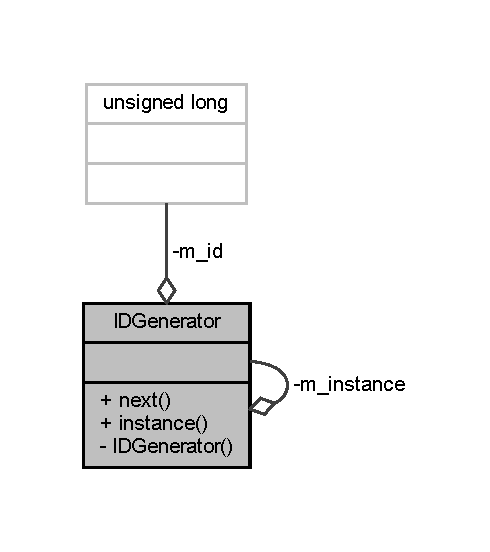
\includegraphics[width=235pt]{class_i_d_generator__coll__graph}
\end{center}
\end{figure}
\doxysubsection*{Public Member Functions}
\begin{DoxyCompactItemize}
\item 
unsigned long \mbox{\hyperlink{class_i_d_generator_a99d8cabb2ec6a17888a8ccbe9c85fee0}{next}} ()
\end{DoxyCompactItemize}
\doxysubsection*{Static Public Member Functions}
\begin{DoxyCompactItemize}
\item 
static \mbox{\hyperlink{class_i_d_generator}{I\+D\+Generator}} $\ast$ \mbox{\hyperlink{class_i_d_generator_ad852c6dadc89e1020e4b3932f5a97bb3}{instance}} ()
\end{DoxyCompactItemize}
\doxysubsection*{Private Member Functions}
\begin{DoxyCompactItemize}
\item 
\mbox{\hyperlink{class_i_d_generator_a8209b55f50b469c47f977660a769b1da}{I\+D\+Generator}} ()
\end{DoxyCompactItemize}
\doxysubsection*{Private Attributes}
\begin{DoxyCompactItemize}
\item 
unsigned long \mbox{\hyperlink{class_i_d_generator_ad0400380525f694b23ff675f4f170893}{m\+\_\+id}}
\end{DoxyCompactItemize}
\doxysubsection*{Static Private Attributes}
\begin{DoxyCompactItemize}
\item 
static \mbox{\hyperlink{class_i_d_generator}{I\+D\+Generator}} $\ast$ \mbox{\hyperlink{class_i_d_generator_a316bacdda67f4cf9bf73fcbd9bf94245}{m\+\_\+instance}}
\end{DoxyCompactItemize}


\doxysubsection{Detailed Description}
This singleton class is used to generate unique identifiers for all agents in the simulation. The identifiers are unsigned long integers. 

\doxysubsection{Constructor \& Destructor Documentation}
\mbox{\Hypertarget{class_i_d_generator_a8209b55f50b469c47f977660a769b1da}\label{class_i_d_generator_a8209b55f50b469c47f977660a769b1da}} 
\index{IDGenerator@{IDGenerator}!IDGenerator@{IDGenerator}}
\index{IDGenerator@{IDGenerator}!IDGenerator@{IDGenerator}}
\doxysubsubsection{\texorpdfstring{IDGenerator()}{IDGenerator()}}
{\footnotesize\ttfamily I\+D\+Generator\+::\+I\+D\+Generator (\begin{DoxyParamCaption}{ }\end{DoxyParamCaption})\hspace{0.3cm}{\ttfamily [inline]}, {\ttfamily [private]}}

Here is the caller graph for this function\+:\nopagebreak
\begin{figure}[H]
\begin{center}
\leavevmode
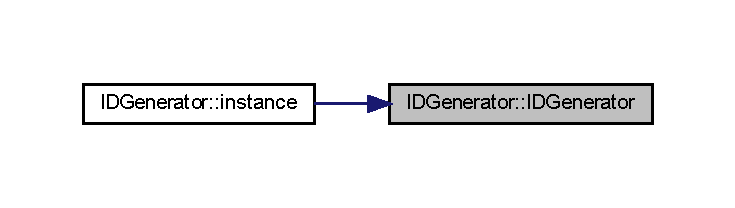
\includegraphics[width=350pt]{class_i_d_generator_a8209b55f50b469c47f977660a769b1da_icgraph}
\end{center}
\end{figure}


\doxysubsection{Member Function Documentation}
\mbox{\Hypertarget{class_i_d_generator_ad852c6dadc89e1020e4b3932f5a97bb3}\label{class_i_d_generator_ad852c6dadc89e1020e4b3932f5a97bb3}} 
\index{IDGenerator@{IDGenerator}!instance@{instance}}
\index{instance@{instance}!IDGenerator@{IDGenerator}}
\doxysubsubsection{\texorpdfstring{instance()}{instance()}}
{\footnotesize\ttfamily static \mbox{\hyperlink{class_i_d_generator}{I\+D\+Generator}}$\ast$ I\+D\+Generator\+::instance (\begin{DoxyParamCaption}{ }\end{DoxyParamCaption})\hspace{0.3cm}{\ttfamily [inline]}, {\ttfamily [static]}}

Returns an instance of this class. \begin{DoxyReturn}{Returns}
an instance of this class. 
\end{DoxyReturn}
Here is the call graph for this function\+:\nopagebreak
\begin{figure}[H]
\begin{center}
\leavevmode
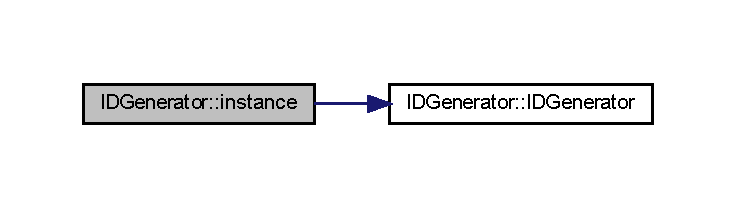
\includegraphics[width=350pt]{class_i_d_generator_ad852c6dadc89e1020e4b3932f5a97bb3_cgraph}
\end{center}
\end{figure}
\mbox{\Hypertarget{class_i_d_generator_a99d8cabb2ec6a17888a8ccbe9c85fee0}\label{class_i_d_generator_a99d8cabb2ec6a17888a8ccbe9c85fee0}} 
\index{IDGenerator@{IDGenerator}!next@{next}}
\index{next@{next}!IDGenerator@{IDGenerator}}
\doxysubsubsection{\texorpdfstring{next()}{next()}}
{\footnotesize\ttfamily unsigned long I\+D\+Generator\+::next (\begin{DoxyParamCaption}{ }\end{DoxyParamCaption})\hspace{0.3cm}{\ttfamily [inline]}}

Generates the next unique identifier. \begin{DoxyReturn}{Returns}
a unique identifier. 
\end{DoxyReturn}


\doxysubsection{Member Data Documentation}
\mbox{\Hypertarget{class_i_d_generator_ad0400380525f694b23ff675f4f170893}\label{class_i_d_generator_ad0400380525f694b23ff675f4f170893}} 
\index{IDGenerator@{IDGenerator}!m\_id@{m\_id}}
\index{m\_id@{m\_id}!IDGenerator@{IDGenerator}}
\doxysubsubsection{\texorpdfstring{m\_id}{m\_id}}
{\footnotesize\ttfamily unsigned long I\+D\+Generator\+::m\+\_\+id\hspace{0.3cm}{\ttfamily [private]}}

\mbox{\Hypertarget{class_i_d_generator_a316bacdda67f4cf9bf73fcbd9bf94245}\label{class_i_d_generator_a316bacdda67f4cf9bf73fcbd9bf94245}} 
\index{IDGenerator@{IDGenerator}!m\_instance@{m\_instance}}
\index{m\_instance@{m\_instance}!IDGenerator@{IDGenerator}}
\doxysubsubsection{\texorpdfstring{m\_instance}{m\_instance}}
{\footnotesize\ttfamily \mbox{\hyperlink{class_i_d_generator}{I\+D\+Generator}}$\ast$ I\+D\+Generator\+::m\+\_\+instance\hspace{0.3cm}{\ttfamily [static]}, {\ttfamily [private]}}



The documentation for this class was generated from the following file\+:\begin{DoxyCompactItemize}
\item 
include/\mbox{\hyperlink{_i_d_generator_8h}{I\+D\+Generator.\+h}}\end{DoxyCompactItemize}

\hypertarget{class_immovable_agent}{}\section{Immovable\+Agent Class Reference}
\label{class_immovable_agent}\index{Immovable\+Agent@{Immovable\+Agent}}


Inheritance diagram for Immovable\+Agent\+:\nopagebreak
\begin{figure}[H]
\begin{center}
\leavevmode
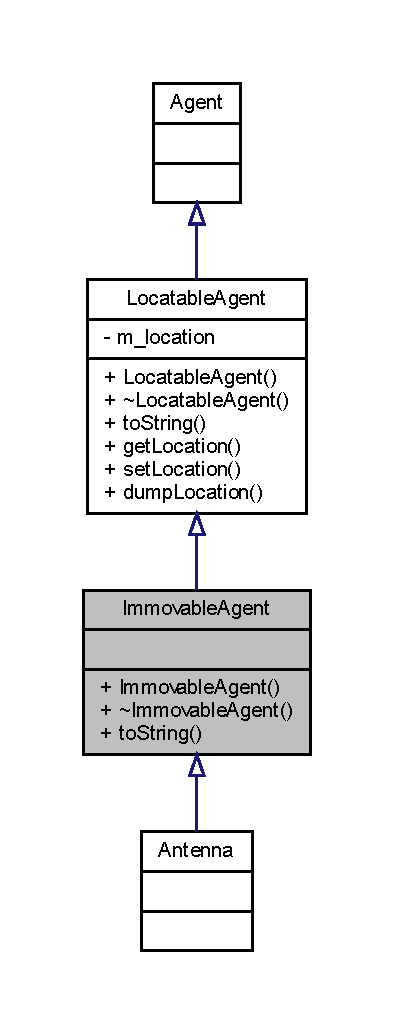
\includegraphics[width=189pt]{class_immovable_agent__inherit__graph}
\end{center}
\end{figure}


Collaboration diagram for Immovable\+Agent\+:\nopagebreak
\begin{figure}[H]
\begin{center}
\leavevmode
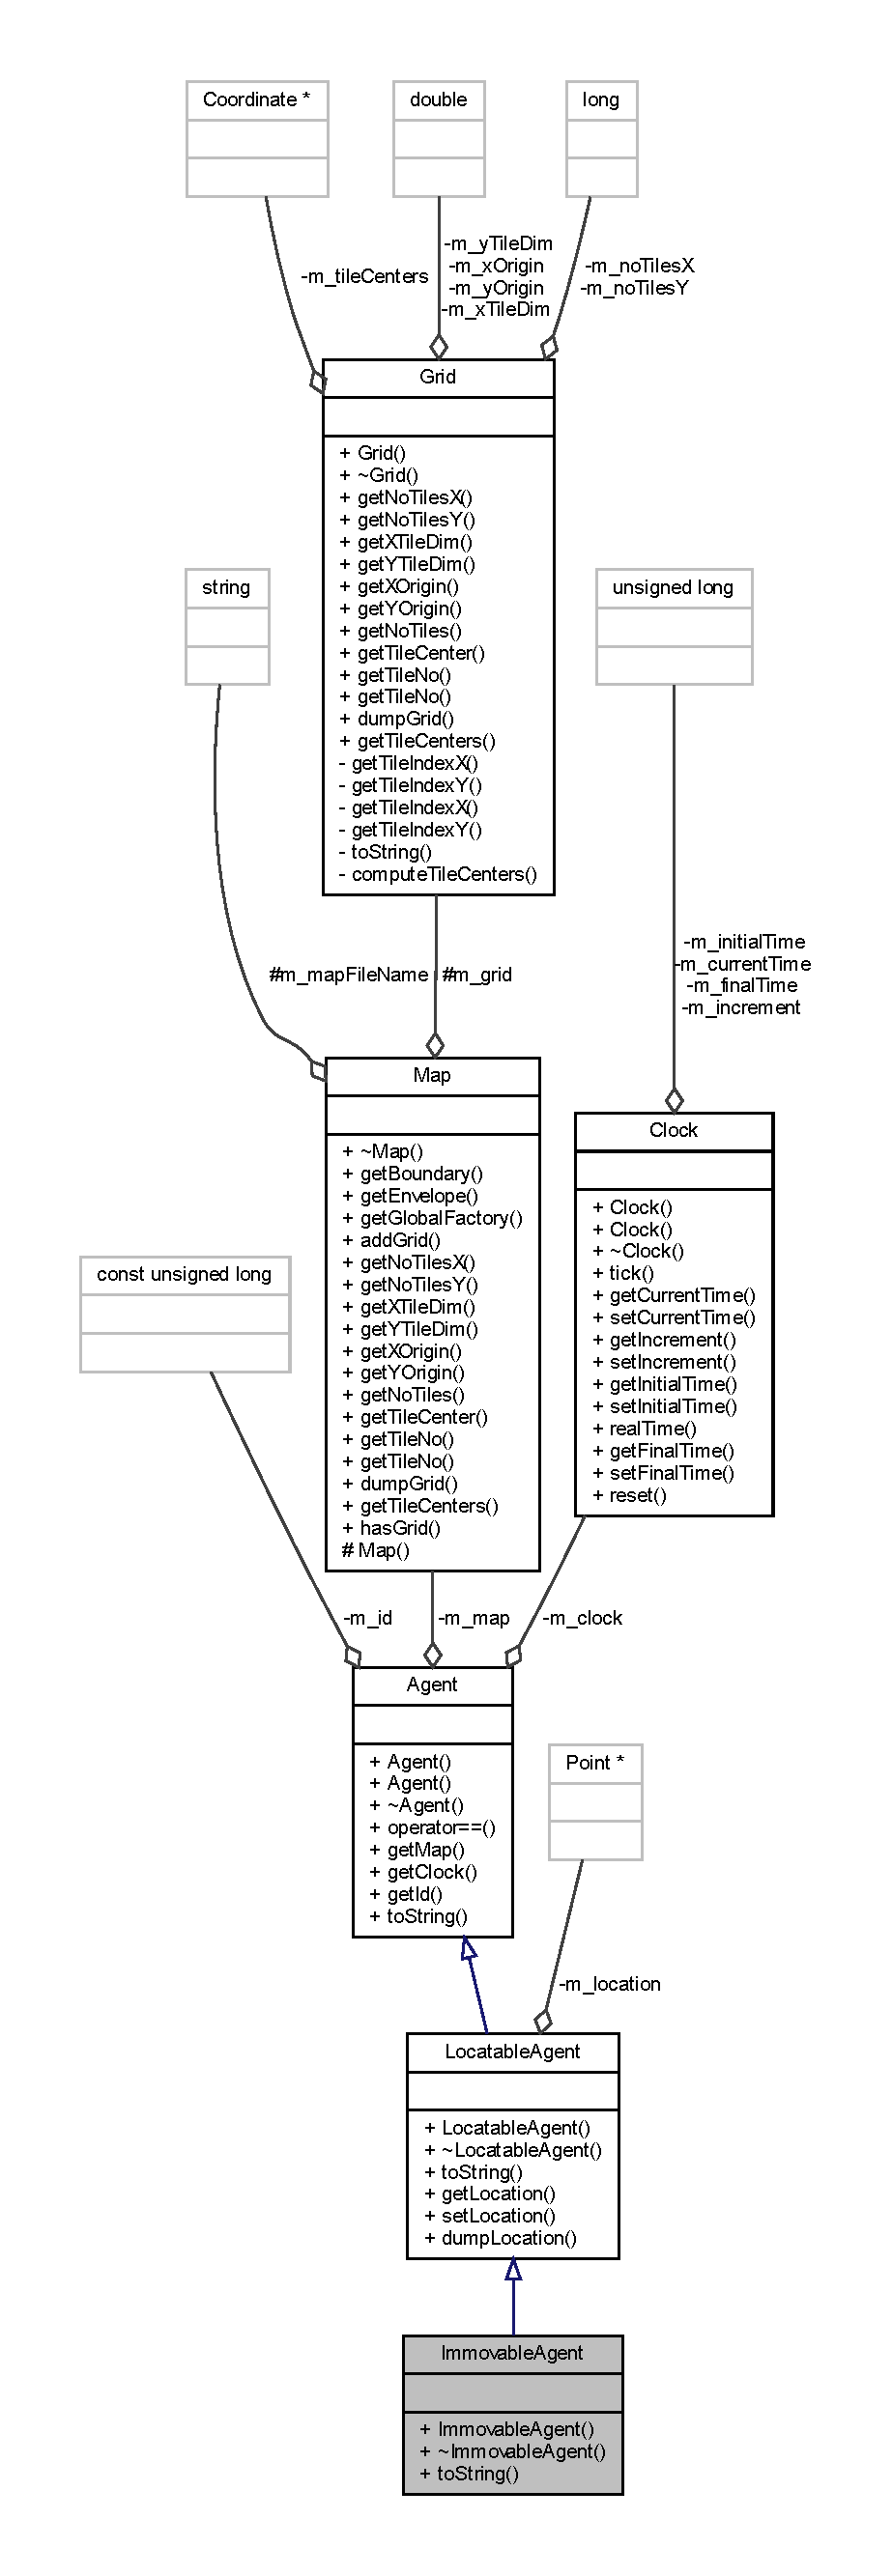
\includegraphics[width=208pt]{class_immovable_agent__coll__graph}
\end{center}
\end{figure}


The documentation for this class was generated from the following file\+:\begin{DoxyCompactItemize}
\item 
include/agent/\hyperlink{_antenna_8h}{Antenna.\+h}\end{DoxyCompactItemize}

\hypertarget{class_input_parser}{}\section{Input\+Parser Class Reference}
\label{class_input_parser}\index{Input\+Parser@{Input\+Parser}}


{\ttfamily \#include $<$Input\+Parser.\+h$>$}



Collaboration diagram for Input\+Parser\+:\nopagebreak
\begin{figure}[H]
\begin{center}
\leavevmode
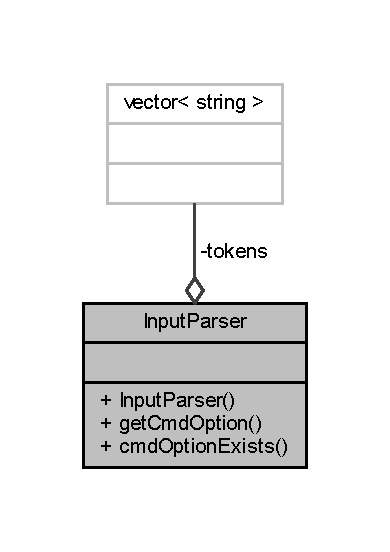
\includegraphics[width=187pt]{class_input_parser__coll__graph}
\end{center}
\end{figure}
\subsection*{Public Member Functions}
\begin{DoxyCompactItemize}
\item 
\hyperlink{class_input_parser_af9fa5ead1f28b5294a713410df5b9531}{Input\+Parser} (int \&argc, char $\ast$$\ast$argv)
\item 
const string \& \hyperlink{class_input_parser_aac05d7ad7794084907a0b57ab3e7d607}{get\+Cmd\+Option} (const string \&option) const
\item 
bool \hyperlink{class_input_parser_ad3d06a9c59e91f425295bdc8408e0544}{cmd\+Option\+Exists} (const string \&option) const
\end{DoxyCompactItemize}
\subsection*{Private Attributes}
\begin{DoxyCompactItemize}
\item 
vector$<$ string $>$ \hyperlink{class_input_parser_a4bd1105d6fc64bd0e825dc2e34515d75}{tokens}
\end{DoxyCompactItemize}


\subsection{Detailed Description}
Utility class used to parse the command line and extract the parameters and their values. An option is passed with a \char`\"{}-\/\char`\"{} sign in front of it. Example\+: \$simulator -\/s simulation.\+xml -\/p persons Here -\/s and -\/p are options and simulation.\+xml and persons.\+xml are their corresponding values. 

\subsection{Constructor \& Destructor Documentation}
\mbox{\Hypertarget{class_input_parser_af9fa5ead1f28b5294a713410df5b9531}\label{class_input_parser_af9fa5ead1f28b5294a713410df5b9531}} 
\index{Input\+Parser@{Input\+Parser}!Input\+Parser@{Input\+Parser}}
\index{Input\+Parser@{Input\+Parser}!Input\+Parser@{Input\+Parser}}
\subsubsection{\texorpdfstring{Input\+Parser()}{InputParser()}}
{\footnotesize\ttfamily Input\+Parser\+::\+Input\+Parser (\begin{DoxyParamCaption}\item[{int \&}]{argc,  }\item[{char $\ast$$\ast$}]{argv }\end{DoxyParamCaption})}

Constructor of the class. 
\begin{DoxyParams}{Parameters}
{\em argc} & the number of the arguments from the command line. \\
\hline
{\em argv} & an array with the parameters passed in the command line. \\
\hline
\end{DoxyParams}


\subsection{Member Function Documentation}
\mbox{\Hypertarget{class_input_parser_ad3d06a9c59e91f425295bdc8408e0544}\label{class_input_parser_ad3d06a9c59e91f425295bdc8408e0544}} 
\index{Input\+Parser@{Input\+Parser}!cmd\+Option\+Exists@{cmd\+Option\+Exists}}
\index{cmd\+Option\+Exists@{cmd\+Option\+Exists}!Input\+Parser@{Input\+Parser}}
\subsubsection{\texorpdfstring{cmd\+Option\+Exists()}{cmdOptionExists()}}
{\footnotesize\ttfamily bool Input\+Parser\+::cmd\+Option\+Exists (\begin{DoxyParamCaption}\item[{const string \&}]{option }\end{DoxyParamCaption}) const}

Checks if an option was passed as a command line parameter. 
\begin{DoxyParams}{Parameters}
{\em option} & the option that we are checking. \\
\hline
\end{DoxyParams}
\begin{DoxyReturn}{Returns}
true if the option is present in the command line, false otherwise. 
\end{DoxyReturn}
\mbox{\Hypertarget{class_input_parser_aac05d7ad7794084907a0b57ab3e7d607}\label{class_input_parser_aac05d7ad7794084907a0b57ab3e7d607}} 
\index{Input\+Parser@{Input\+Parser}!get\+Cmd\+Option@{get\+Cmd\+Option}}
\index{get\+Cmd\+Option@{get\+Cmd\+Option}!Input\+Parser@{Input\+Parser}}
\subsubsection{\texorpdfstring{get\+Cmd\+Option()}{getCmdOption()}}
{\footnotesize\ttfamily const string\& Input\+Parser\+::get\+Cmd\+Option (\begin{DoxyParamCaption}\item[{const string \&}]{option }\end{DoxyParamCaption}) const}

Returns the value of an option passed as a command line parameter. 
\begin{DoxyParams}{Parameters}
{\em option} & an option from the command line. \\
\hline
\end{DoxyParams}
\begin{DoxyReturn}{Returns}
the value of the option passed as a command line parameter. 
\end{DoxyReturn}


\subsection{Member Data Documentation}
\mbox{\Hypertarget{class_input_parser_a4bd1105d6fc64bd0e825dc2e34515d75}\label{class_input_parser_a4bd1105d6fc64bd0e825dc2e34515d75}} 
\index{Input\+Parser@{Input\+Parser}!tokens@{tokens}}
\index{tokens@{tokens}!Input\+Parser@{Input\+Parser}}
\subsubsection{\texorpdfstring{tokens}{tokens}}
{\footnotesize\ttfamily vector$<$string$>$ Input\+Parser\+::tokens\hspace{0.3cm}{\ttfamily [private]}}



The documentation for this class was generated from the following file\+:\begin{DoxyCompactItemize}
\item 
include/\hyperlink{_input_parser_8h}{Input\+Parser.\+h}\end{DoxyCompactItemize}

\hypertarget{class_age_distribution_1_1_it}{}\doxysection{It Class Reference}
\label{class_age_distribution_1_1_it}\index{It@{It}}


Collaboration diagram for It\+:\nopagebreak
\begin{figure}[H]
\begin{center}
\leavevmode
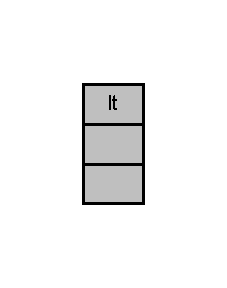
\includegraphics[width=109pt]{class_age_distribution_1_1_it__coll__graph}
\end{center}
\end{figure}


\doxysubsection{Detailed Description}
Subclass of the truncated normal distribution.

Subclass of the uniform distribution. 

The documentation for this class was generated from the following file\+:\begin{DoxyCompactItemize}
\item 
include/\mbox{\hyperlink{_truncated_normal_age_distribution_8h}{Truncated\+Normal\+Age\+Distribution.\+h}}\end{DoxyCompactItemize}

\hypertarget{class_levy_flight_displacement}{}\doxysection{Levy\+Flight\+Displacement Class Reference}
\label{class_levy_flight_displacement}\index{LevyFlightDisplacement@{LevyFlightDisplacement}}


{\ttfamily \#include $<$Levy\+Flight\+Displacement.\+h$>$}



Inheritance diagram for Levy\+Flight\+Displacement\+:\nopagebreak
\begin{figure}[H]
\begin{center}
\leavevmode
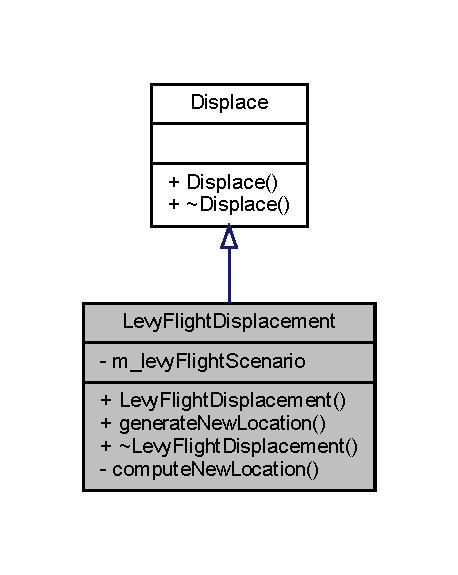
\includegraphics[width=220pt]{class_levy_flight_displacement__inherit__graph}
\end{center}
\end{figure}


Collaboration diagram for Levy\+Flight\+Displacement\+:\nopagebreak
\begin{figure}[H]
\begin{center}
\leavevmode
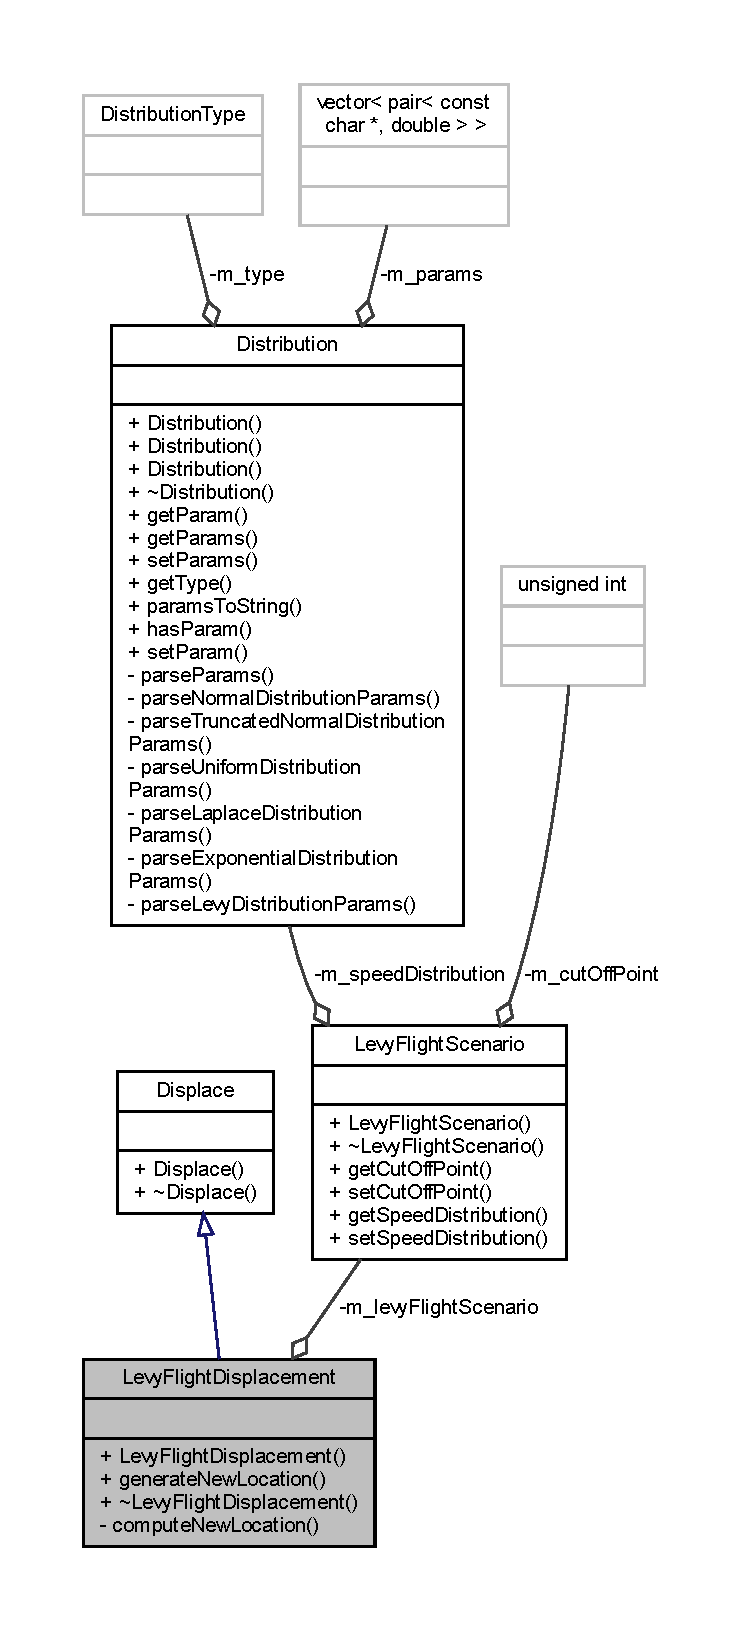
\includegraphics[height=550pt]{class_levy_flight_displacement__coll__graph}
\end{center}
\end{figure}
\doxysubsection*{Public Member Functions}
\begin{DoxyCompactItemize}
\item 
\mbox{\hyperlink{class_levy_flight_displacement_ae807b06a0d81cf1f703c41c480a5a02f}{Levy\+Flight\+Displacement}} (\mbox{\hyperlink{class_simulation_configuration}{Simulation\+Configuration}} $\ast$sim\+Config, double speed)
\item 
virtual Point $\ast$ \mbox{\hyperlink{class_levy_flight_displacement_ae9b877b962cfbab65ba538da0e10b0f7}{generate\+New\+Location}} (Point $\ast$p) override
\item 
virtual \mbox{\hyperlink{class_levy_flight_displacement_ac5a53d10d6b3e30b96e1ccc91a1b448e}{$\sim$\+Levy\+Flight\+Displacement}} ()
\end{DoxyCompactItemize}
\doxysubsection*{Private Member Functions}
\begin{DoxyCompactItemize}
\item 
virtual Point $\ast$ \mbox{\hyperlink{class_levy_flight_displacement_af95a25afc1f0f29a0e0e01e144925183}{compute\+New\+Location}} (Point $\ast$init\+Location, double theta) override
\end{DoxyCompactItemize}
\doxysubsection*{Private Attributes}
\begin{DoxyCompactItemize}
\item 
\mbox{\hyperlink{class_levy_flight_scenario}{Levy\+Flight\+Scenario}} $\ast$ \mbox{\hyperlink{class_levy_flight_displacement_a52c76c9dee0a2b241cf44c5c7307cd97}{m\+\_\+levy\+Flight\+Scenario}}
\end{DoxyCompactItemize}


\doxysubsection{Detailed Description}
This class is part of the Strategy design pattern used to implement the displacement of persons on the map. It implements the Levy flights, overriding the \mbox{\hyperlink{class_levy_flight_displacement_ae9b877b962cfbab65ba538da0e10b0f7}{generate\+New\+Location()}} method from its superclass, \mbox{\hyperlink{class_displace}{Displace}}. 

\doxysubsection{Constructor \& Destructor Documentation}
\mbox{\Hypertarget{class_levy_flight_displacement_ae807b06a0d81cf1f703c41c480a5a02f}\label{class_levy_flight_displacement_ae807b06a0d81cf1f703c41c480a5a02f}} 
\index{LevyFlightDisplacement@{LevyFlightDisplacement}!LevyFlightDisplacement@{LevyFlightDisplacement}}
\index{LevyFlightDisplacement@{LevyFlightDisplacement}!LevyFlightDisplacement@{LevyFlightDisplacement}}
\doxysubsubsection{\texorpdfstring{LevyFlightDisplacement()}{LevyFlightDisplacement()}}
{\footnotesize\ttfamily Levy\+Flight\+Displacement\+::\+Levy\+Flight\+Displacement (\begin{DoxyParamCaption}\item[{\mbox{\hyperlink{class_simulation_configuration}{Simulation\+Configuration}} $\ast$}]{sim\+Config,  }\item[{double}]{speed }\end{DoxyParamCaption})}

Constructor of the class. It only passes the arguments to the superclass, \mbox{\hyperlink{class_displace}{Displace}}. 
\begin{DoxyParams}{Parameters}
{\em speed} & the speed of displacement. \\
\hline
\end{DoxyParams}
\mbox{\Hypertarget{class_levy_flight_displacement_ac5a53d10d6b3e30b96e1ccc91a1b448e}\label{class_levy_flight_displacement_ac5a53d10d6b3e30b96e1ccc91a1b448e}} 
\index{LevyFlightDisplacement@{LevyFlightDisplacement}!````~LevyFlightDisplacement@{$\sim$LevyFlightDisplacement}}
\index{````~LevyFlightDisplacement@{$\sim$LevyFlightDisplacement}!LevyFlightDisplacement@{LevyFlightDisplacement}}
\doxysubsubsection{\texorpdfstring{$\sim$LevyFlightDisplacement()}{~LevyFlightDisplacement()}}
{\footnotesize\ttfamily virtual Levy\+Flight\+Displacement\+::$\sim$\+Levy\+Flight\+Displacement (\begin{DoxyParamCaption}{ }\end{DoxyParamCaption})\hspace{0.3cm}{\ttfamily [virtual]}}

Destructor. Does nothing. 

\doxysubsection{Member Function Documentation}
\mbox{\Hypertarget{class_levy_flight_displacement_af95a25afc1f0f29a0e0e01e144925183}\label{class_levy_flight_displacement_af95a25afc1f0f29a0e0e01e144925183}} 
\index{LevyFlightDisplacement@{LevyFlightDisplacement}!computeNewLocation@{computeNewLocation}}
\index{computeNewLocation@{computeNewLocation}!LevyFlightDisplacement@{LevyFlightDisplacement}}
\doxysubsubsection{\texorpdfstring{computeNewLocation()}{computeNewLocation()}}
{\footnotesize\ttfamily virtual Point$\ast$ Levy\+Flight\+Displacement\+::compute\+New\+Location (\begin{DoxyParamCaption}\item[{Point $\ast$}]{init\+Location,  }\item[{double}]{theta }\end{DoxyParamCaption})\hspace{0.3cm}{\ttfamily [override]}, {\ttfamily [private]}, {\ttfamily [virtual]}}

\mbox{\Hypertarget{class_levy_flight_displacement_ae9b877b962cfbab65ba538da0e10b0f7}\label{class_levy_flight_displacement_ae9b877b962cfbab65ba538da0e10b0f7}} 
\index{LevyFlightDisplacement@{LevyFlightDisplacement}!generateNewLocation@{generateNewLocation}}
\index{generateNewLocation@{generateNewLocation}!LevyFlightDisplacement@{LevyFlightDisplacement}}
\doxysubsubsection{\texorpdfstring{generateNewLocation()}{generateNewLocation()}}
{\footnotesize\ttfamily virtual Point$\ast$ Levy\+Flight\+Displacement\+::generate\+New\+Location (\begin{DoxyParamCaption}\item[{Point $\ast$}]{p }\end{DoxyParamCaption})\hspace{0.3cm}{\ttfamily [override]}, {\ttfamily [virtual]}}

Implements the Levy flight behavior. It takes a pointer to the current location, generates a uniformly distributed value between 0 and 2$\ast$\+PI as the angle of displacement and computes the length of the step in this direction using the speed and the time duration of a simulation step. To simulate a Levy flight, the value of the speed is generated at each time instant from a Levy distribution. If the new location is outside the map, it tries 10 times to generate another location. If after 10 trials the position is still outside the map returns the current location, i.\+e. the object will stay in the same location until the next simulation step. 
\begin{DoxyParams}{Parameters}
{\em p} & a pointer to the current location. \\
\hline
\end{DoxyParams}
\begin{DoxyReturn}{Returns}
the new location 
\end{DoxyReturn}


\doxysubsection{Member Data Documentation}
\mbox{\Hypertarget{class_levy_flight_displacement_a52c76c9dee0a2b241cf44c5c7307cd97}\label{class_levy_flight_displacement_a52c76c9dee0a2b241cf44c5c7307cd97}} 
\index{LevyFlightDisplacement@{LevyFlightDisplacement}!m\_levyFlightScenario@{m\_levyFlightScenario}}
\index{m\_levyFlightScenario@{m\_levyFlightScenario}!LevyFlightDisplacement@{LevyFlightDisplacement}}
\doxysubsubsection{\texorpdfstring{m\_levyFlightScenario}{m\_levyFlightScenario}}
{\footnotesize\ttfamily \mbox{\hyperlink{class_levy_flight_scenario}{Levy\+Flight\+Scenario}}$\ast$ Levy\+Flight\+Displacement\+::m\+\_\+levy\+Flight\+Scenario\hspace{0.3cm}{\ttfamily [private]}}



The documentation for this class was generated from the following file\+:\begin{DoxyCompactItemize}
\item 
include/\mbox{\hyperlink{_levy_flight_displacement_8h}{Levy\+Flight\+Displacement.\+h}}\end{DoxyCompactItemize}

\hypertarget{class_levy_flight_scenario}{}\doxysection{Levy\+Flight\+Scenario Class Reference}
\label{class_levy_flight_scenario}\index{LevyFlightScenario@{LevyFlightScenario}}


{\ttfamily \#include $<$Levy\+Flight\+Scenario.\+h$>$}



Collaboration diagram for Levy\+Flight\+Scenario\+:\nopagebreak
\begin{figure}[H]
\begin{center}
\leavevmode
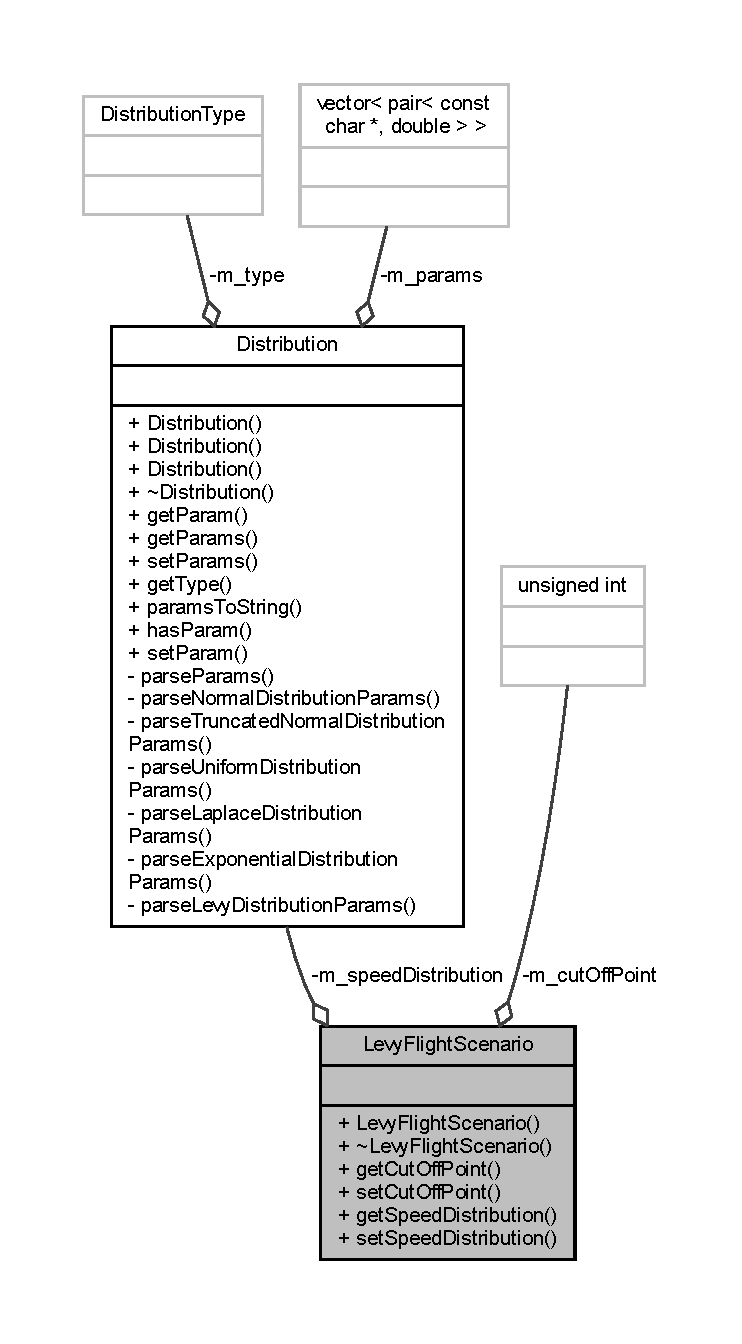
\includegraphics[height=550pt]{class_levy_flight_scenario__coll__graph}
\end{center}
\end{figure}
\doxysubsection*{Public Member Functions}
\begin{DoxyCompactItemize}
\item 
\mbox{\hyperlink{class_levy_flight_scenario_a62d4c67e6263c33820148a41b2c3e8c9}{Levy\+Flight\+Scenario}} ()
\item 
virtual \mbox{\hyperlink{class_levy_flight_scenario_adbd40b256f875fe19f35ccb57177add7}{$\sim$\+Levy\+Flight\+Scenario}} ()
\item 
unsigned int \mbox{\hyperlink{class_levy_flight_scenario_a7433446b18d145ba8a53f3ddcfcb59d2}{get\+Cut\+Off\+Point}} () const
\item 
void \mbox{\hyperlink{class_levy_flight_scenario_ad43b978b98ed9e8ff17437aff5cd7619}{set\+Cut\+Off\+Point}} (unsigned int cut\+Off\+Point)
\item 
\mbox{\hyperlink{class_distribution}{Distribution}} $\ast$ \mbox{\hyperlink{class_levy_flight_scenario_a343a976575ca830901d7e4da73aa820f}{get\+Speed\+Distribution}} () const
\item 
void \mbox{\hyperlink{class_levy_flight_scenario_a469a4d56e885e5ee929297133672c887}{set\+Speed\+Distribution}} (\mbox{\hyperlink{class_distribution}{Distribution}} $\ast$speed\+Distribution)
\end{DoxyCompactItemize}
\doxysubsection*{Private Attributes}
\begin{DoxyCompactItemize}
\item 
\mbox{\hyperlink{class_distribution}{Distribution}} $\ast$ \mbox{\hyperlink{class_levy_flight_scenario_ace30c70c8e2cea1aad5ec3f7285e1b38}{m\+\_\+speed\+Distribution}}
\item 
unsigned int \mbox{\hyperlink{class_levy_flight_scenario_aa8a42ec9a71336e18eedf2769c220448}{m\+\_\+cut\+Off\+Point}}
\end{DoxyCompactItemize}


\doxysubsection{Constructor \& Destructor Documentation}
\mbox{\Hypertarget{class_levy_flight_scenario_a62d4c67e6263c33820148a41b2c3e8c9}\label{class_levy_flight_scenario_a62d4c67e6263c33820148a41b2c3e8c9}} 
\index{LevyFlightScenario@{LevyFlightScenario}!LevyFlightScenario@{LevyFlightScenario}}
\index{LevyFlightScenario@{LevyFlightScenario}!LevyFlightScenario@{LevyFlightScenario}}
\doxysubsubsection{\texorpdfstring{LevyFlightScenario()}{LevyFlightScenario()}}
{\footnotesize\ttfamily Levy\+Flight\+Scenario\+::\+Levy\+Flight\+Scenario (\begin{DoxyParamCaption}{ }\end{DoxyParamCaption})}

\mbox{\Hypertarget{class_levy_flight_scenario_adbd40b256f875fe19f35ccb57177add7}\label{class_levy_flight_scenario_adbd40b256f875fe19f35ccb57177add7}} 
\index{LevyFlightScenario@{LevyFlightScenario}!````~LevyFlightScenario@{$\sim$LevyFlightScenario}}
\index{````~LevyFlightScenario@{$\sim$LevyFlightScenario}!LevyFlightScenario@{LevyFlightScenario}}
\doxysubsubsection{\texorpdfstring{$\sim$LevyFlightScenario()}{~LevyFlightScenario()}}
{\footnotesize\ttfamily virtual Levy\+Flight\+Scenario\+::$\sim$\+Levy\+Flight\+Scenario (\begin{DoxyParamCaption}{ }\end{DoxyParamCaption})\hspace{0.3cm}{\ttfamily [virtual]}}



\doxysubsection{Member Function Documentation}
\mbox{\Hypertarget{class_levy_flight_scenario_a7433446b18d145ba8a53f3ddcfcb59d2}\label{class_levy_flight_scenario_a7433446b18d145ba8a53f3ddcfcb59d2}} 
\index{LevyFlightScenario@{LevyFlightScenario}!getCutOffPoint@{getCutOffPoint}}
\index{getCutOffPoint@{getCutOffPoint}!LevyFlightScenario@{LevyFlightScenario}}
\doxysubsubsection{\texorpdfstring{getCutOffPoint()}{getCutOffPoint()}}
{\footnotesize\ttfamily unsigned int Levy\+Flight\+Scenario\+::get\+Cut\+Off\+Point (\begin{DoxyParamCaption}{ }\end{DoxyParamCaption}) const}

\mbox{\Hypertarget{class_levy_flight_scenario_a343a976575ca830901d7e4da73aa820f}\label{class_levy_flight_scenario_a343a976575ca830901d7e4da73aa820f}} 
\index{LevyFlightScenario@{LevyFlightScenario}!getSpeedDistribution@{getSpeedDistribution}}
\index{getSpeedDistribution@{getSpeedDistribution}!LevyFlightScenario@{LevyFlightScenario}}
\doxysubsubsection{\texorpdfstring{getSpeedDistribution()}{getSpeedDistribution()}}
{\footnotesize\ttfamily \mbox{\hyperlink{class_distribution}{Distribution}}$\ast$ Levy\+Flight\+Scenario\+::get\+Speed\+Distribution (\begin{DoxyParamCaption}{ }\end{DoxyParamCaption}) const}

\mbox{\Hypertarget{class_levy_flight_scenario_ad43b978b98ed9e8ff17437aff5cd7619}\label{class_levy_flight_scenario_ad43b978b98ed9e8ff17437aff5cd7619}} 
\index{LevyFlightScenario@{LevyFlightScenario}!setCutOffPoint@{setCutOffPoint}}
\index{setCutOffPoint@{setCutOffPoint}!LevyFlightScenario@{LevyFlightScenario}}
\doxysubsubsection{\texorpdfstring{setCutOffPoint()}{setCutOffPoint()}}
{\footnotesize\ttfamily void Levy\+Flight\+Scenario\+::set\+Cut\+Off\+Point (\begin{DoxyParamCaption}\item[{unsigned int}]{cut\+Off\+Point }\end{DoxyParamCaption})}

\mbox{\Hypertarget{class_levy_flight_scenario_a469a4d56e885e5ee929297133672c887}\label{class_levy_flight_scenario_a469a4d56e885e5ee929297133672c887}} 
\index{LevyFlightScenario@{LevyFlightScenario}!setSpeedDistribution@{setSpeedDistribution}}
\index{setSpeedDistribution@{setSpeedDistribution}!LevyFlightScenario@{LevyFlightScenario}}
\doxysubsubsection{\texorpdfstring{setSpeedDistribution()}{setSpeedDistribution()}}
{\footnotesize\ttfamily void Levy\+Flight\+Scenario\+::set\+Speed\+Distribution (\begin{DoxyParamCaption}\item[{\mbox{\hyperlink{class_distribution}{Distribution}} $\ast$}]{speed\+Distribution }\end{DoxyParamCaption})}



\doxysubsection{Member Data Documentation}
\mbox{\Hypertarget{class_levy_flight_scenario_aa8a42ec9a71336e18eedf2769c220448}\label{class_levy_flight_scenario_aa8a42ec9a71336e18eedf2769c220448}} 
\index{LevyFlightScenario@{LevyFlightScenario}!m\_cutOffPoint@{m\_cutOffPoint}}
\index{m\_cutOffPoint@{m\_cutOffPoint}!LevyFlightScenario@{LevyFlightScenario}}
\doxysubsubsection{\texorpdfstring{m\_cutOffPoint}{m\_cutOffPoint}}
{\footnotesize\ttfamily unsigned int Levy\+Flight\+Scenario\+::m\+\_\+cut\+Off\+Point\hspace{0.3cm}{\ttfamily [private]}}

\mbox{\Hypertarget{class_levy_flight_scenario_ace30c70c8e2cea1aad5ec3f7285e1b38}\label{class_levy_flight_scenario_ace30c70c8e2cea1aad5ec3f7285e1b38}} 
\index{LevyFlightScenario@{LevyFlightScenario}!m\_speedDistribution@{m\_speedDistribution}}
\index{m\_speedDistribution@{m\_speedDistribution}!LevyFlightScenario@{LevyFlightScenario}}
\doxysubsubsection{\texorpdfstring{m\_speedDistribution}{m\_speedDistribution}}
{\footnotesize\ttfamily \mbox{\hyperlink{class_distribution}{Distribution}}$\ast$ Levy\+Flight\+Scenario\+::m\+\_\+speed\+Distribution\hspace{0.3cm}{\ttfamily [private]}}



The documentation for this class was generated from the following file\+:\begin{DoxyCompactItemize}
\item 
include/parsers/\mbox{\hyperlink{_levy_flight_scenario_8h}{Levy\+Flight\+Scenario.\+h}}\end{DoxyCompactItemize}

\hypertarget{class_map}{}\doxysection{Map Class Reference}
\label{class_map}\index{Map@{Map}}


{\ttfamily \#include $<$Map.\+h$>$}



Inheritance diagram for Map\+:\nopagebreak
\begin{figure}[H]
\begin{center}
\leavevmode
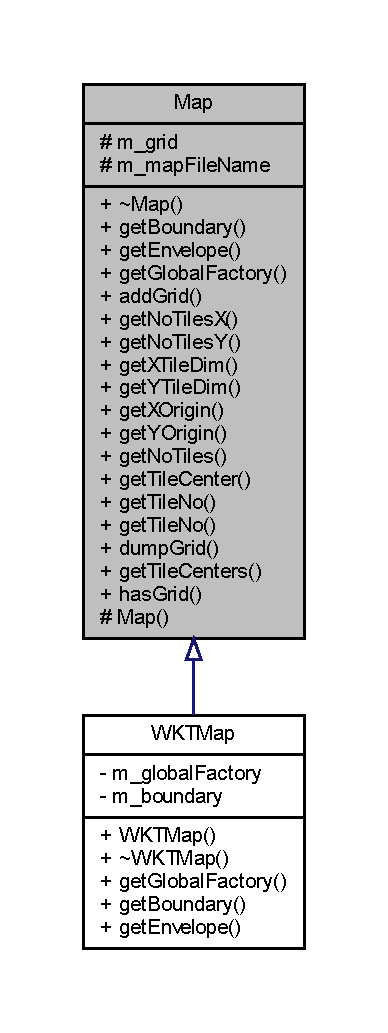
\includegraphics[width=186pt]{class_map__inherit__graph}
\end{center}
\end{figure}


Collaboration diagram for Map\+:\nopagebreak
\begin{figure}[H]
\begin{center}
\leavevmode
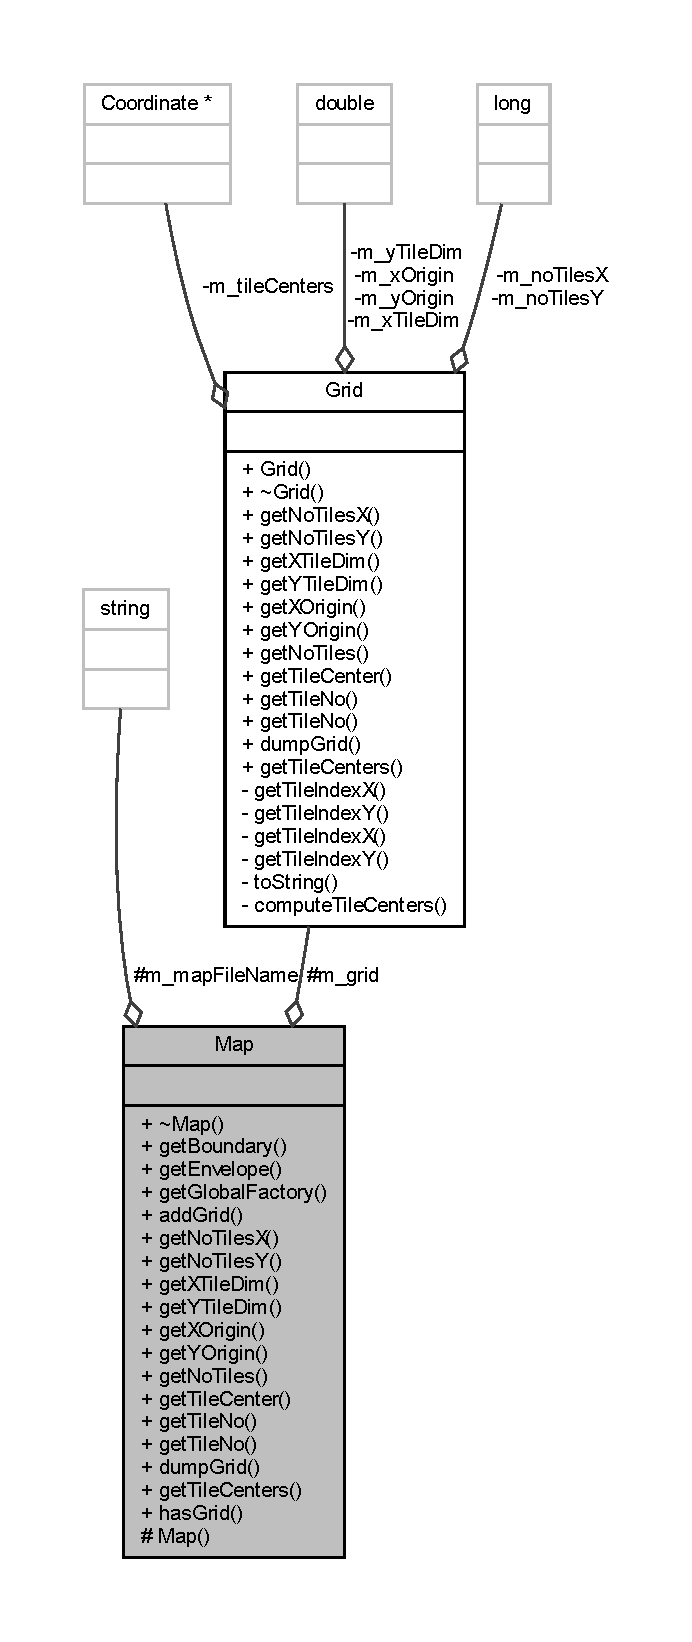
\includegraphics[height=550pt]{class_map__coll__graph}
\end{center}
\end{figure}
\doxysubsection*{Public Member Functions}
\begin{DoxyCompactItemize}
\item 
virtual \mbox{\hyperlink{class_map_ac1ab46138aa61acd0a58b1fd21e0df37}{$\sim$\+Map}} ()
\item 
virtual Geometry $\ast$ \mbox{\hyperlink{class_map_aa6b66dc80060a42151228f3764db539f}{get\+Boundary}} () const =0
\item 
virtual Geometry $\ast$ \mbox{\hyperlink{class_map_a40854af632e83500ca5b44180eae8e87}{get\+Envelope}} () const =0
\item 
const virtual Geometry\+Factory\+::\+Ptr \& \mbox{\hyperlink{class_map_aec5e1dc5a24940811b659f6e22f8b0a0}{get\+Global\+Factory}} () const =0
\item 
virtual void \mbox{\hyperlink{class_map_a24246583fbf3bbed56bfb5cd595f941f}{add\+Grid}} (double dim\+TileX, double dim\+TileY)
\item 
virtual unsigned long \mbox{\hyperlink{class_map_aace69b7294f0da0e2ca000dfa2a29606}{get\+No\+TilesX}} () const
\item 
virtual unsigned long \mbox{\hyperlink{class_map_a13ff108a9b56c432665d36ba1cbad1d0}{get\+No\+TilesY}} () const
\item 
virtual double \mbox{\hyperlink{class_map_a0a7326f8167effc1b6c0329de3c29d60}{get\+X\+Tile\+Dim}} () const
\item 
virtual double \mbox{\hyperlink{class_map_af36385173af71e8e0cd989dceb8f8aea}{get\+Y\+Tile\+Dim}} () const
\item 
virtual double \mbox{\hyperlink{class_map_af3e4dc640ee38ff6e77ab41435fcc42d}{get\+X\+Origin}} () const
\item 
virtual double \mbox{\hyperlink{class_map_a5bf4ef0a81f82df90465136c61a440bc}{get\+Y\+Origin}} () const
\item 
const virtual unsigned long \mbox{\hyperlink{class_map_ac10538e70070d20f09ac90b8cfcef554}{get\+No\+Tiles}} () const
\item 
virtual Coordinate \mbox{\hyperlink{class_map_a3ade598881798896b554f2ba34d8b499}{get\+Tile\+Center}} (unsigned long tile\+Index) const
\item 
virtual unsigned long \mbox{\hyperlink{class_map_af9727bc4d5a77cb35b60d92d0e176171}{get\+Tile\+No}} (const Point $\ast$p) const
\item 
virtual unsigned long \mbox{\hyperlink{class_map_ab68490803824fc485652757d992af18e}{get\+Tile\+No}} (double x, double y) const
\item 
virtual void \mbox{\hyperlink{class_map_afb74aa56fb64f4ab4857269c7924ec5a}{dump\+Grid}} (const string \&grid\+File\+Name) const
\item 
virtual Coordinate $\ast$ \mbox{\hyperlink{class_map_a6ff5cb95191b3a749f9a14b72eba2584}{get\+Tile\+Centers}} () const
\item 
virtual bool \mbox{\hyperlink{class_map_aca471e63e8f9f9a892a5491aee94eada}{has\+Grid}} () const
\end{DoxyCompactItemize}
\doxysubsection*{Protected Member Functions}
\begin{DoxyCompactItemize}
\item 
\mbox{\hyperlink{class_map_aa9b06672216e01d51b96cc4f70d3206d}{Map}} (string map\+File\+Name)
\end{DoxyCompactItemize}
\doxysubsection*{Protected Attributes}
\begin{DoxyCompactItemize}
\item 
\mbox{\hyperlink{class_grid}{Grid}} $\ast$ \mbox{\hyperlink{class_map_a0fc16621dbe307d36170c3a96b24b7d9}{m\+\_\+grid}}
\item 
string \mbox{\hyperlink{class_map_a54e527b86ef517e67b299ef06233addc}{m\+\_\+map\+File\+Name}}
\end{DoxyCompactItemize}


\doxysubsection{Constructor \& Destructor Documentation}
\mbox{\Hypertarget{class_map_ac1ab46138aa61acd0a58b1fd21e0df37}\label{class_map_ac1ab46138aa61acd0a58b1fd21e0df37}} 
\index{Map@{Map}!````~Map@{$\sim$Map}}
\index{````~Map@{$\sim$Map}!Map@{Map}}
\doxysubsubsection{\texorpdfstring{$\sim$Map()}{~Map()}}
{\footnotesize\ttfamily virtual Map\+::$\sim$\+Map (\begin{DoxyParamCaption}{ }\end{DoxyParamCaption})\hspace{0.3cm}{\ttfamily [virtual]}}

\mbox{\Hypertarget{class_map_aa9b06672216e01d51b96cc4f70d3206d}\label{class_map_aa9b06672216e01d51b96cc4f70d3206d}} 
\index{Map@{Map}!Map@{Map}}
\index{Map@{Map}!Map@{Map}}
\doxysubsubsection{\texorpdfstring{Map()}{Map()}}
{\footnotesize\ttfamily Map\+::\+Map (\begin{DoxyParamCaption}\item[{string}]{map\+File\+Name }\end{DoxyParamCaption})\hspace{0.3cm}{\ttfamily [protected]}}



\doxysubsection{Member Function Documentation}
\mbox{\Hypertarget{class_map_a24246583fbf3bbed56bfb5cd595f941f}\label{class_map_a24246583fbf3bbed56bfb5cd595f941f}} 
\index{Map@{Map}!addGrid@{addGrid}}
\index{addGrid@{addGrid}!Map@{Map}}
\doxysubsubsection{\texorpdfstring{addGrid()}{addGrid()}}
{\footnotesize\ttfamily virtual void Map\+::add\+Grid (\begin{DoxyParamCaption}\item[{double}]{dim\+TileX,  }\item[{double}]{dim\+TileY }\end{DoxyParamCaption})\hspace{0.3cm}{\ttfamily [virtual]}}

\mbox{\Hypertarget{class_map_afb74aa56fb64f4ab4857269c7924ec5a}\label{class_map_afb74aa56fb64f4ab4857269c7924ec5a}} 
\index{Map@{Map}!dumpGrid@{dumpGrid}}
\index{dumpGrid@{dumpGrid}!Map@{Map}}
\doxysubsubsection{\texorpdfstring{dumpGrid()}{dumpGrid()}}
{\footnotesize\ttfamily virtual void Map\+::dump\+Grid (\begin{DoxyParamCaption}\item[{const string \&}]{grid\+File\+Name }\end{DoxyParamCaption}) const\hspace{0.3cm}{\ttfamily [virtual]}}

\mbox{\Hypertarget{class_map_aa6b66dc80060a42151228f3764db539f}\label{class_map_aa6b66dc80060a42151228f3764db539f}} 
\index{Map@{Map}!getBoundary@{getBoundary}}
\index{getBoundary@{getBoundary}!Map@{Map}}
\doxysubsubsection{\texorpdfstring{getBoundary()}{getBoundary()}}
{\footnotesize\ttfamily virtual Geometry$\ast$ Map\+::get\+Boundary (\begin{DoxyParamCaption}{ }\end{DoxyParamCaption}) const\hspace{0.3cm}{\ttfamily [pure virtual]}}



Implemented in \mbox{\hyperlink{class_w_k_t_map_a0b326822ab1bcfc0765e97f3acb545b0}{W\+K\+T\+Map}}.

\mbox{\Hypertarget{class_map_a40854af632e83500ca5b44180eae8e87}\label{class_map_a40854af632e83500ca5b44180eae8e87}} 
\index{Map@{Map}!getEnvelope@{getEnvelope}}
\index{getEnvelope@{getEnvelope}!Map@{Map}}
\doxysubsubsection{\texorpdfstring{getEnvelope()}{getEnvelope()}}
{\footnotesize\ttfamily virtual Geometry$\ast$ Map\+::get\+Envelope (\begin{DoxyParamCaption}{ }\end{DoxyParamCaption}) const\hspace{0.3cm}{\ttfamily [pure virtual]}}



Implemented in \mbox{\hyperlink{class_w_k_t_map_af117af8392fc33f1e603f10ea57ac6b0}{W\+K\+T\+Map}}.

\mbox{\Hypertarget{class_map_aec5e1dc5a24940811b659f6e22f8b0a0}\label{class_map_aec5e1dc5a24940811b659f6e22f8b0a0}} 
\index{Map@{Map}!getGlobalFactory@{getGlobalFactory}}
\index{getGlobalFactory@{getGlobalFactory}!Map@{Map}}
\doxysubsubsection{\texorpdfstring{getGlobalFactory()}{getGlobalFactory()}}
{\footnotesize\ttfamily const virtual Geometry\+Factory\+::\+Ptr\& Map\+::get\+Global\+Factory (\begin{DoxyParamCaption}{ }\end{DoxyParamCaption}) const\hspace{0.3cm}{\ttfamily [pure virtual]}}



Implemented in \mbox{\hyperlink{class_w_k_t_map_a566b85bafc53e2013e0a21d4a387ce91}{W\+K\+T\+Map}}.

\mbox{\Hypertarget{class_map_ac10538e70070d20f09ac90b8cfcef554}\label{class_map_ac10538e70070d20f09ac90b8cfcef554}} 
\index{Map@{Map}!getNoTiles@{getNoTiles}}
\index{getNoTiles@{getNoTiles}!Map@{Map}}
\doxysubsubsection{\texorpdfstring{getNoTiles()}{getNoTiles()}}
{\footnotesize\ttfamily const virtual unsigned long Map\+::get\+No\+Tiles (\begin{DoxyParamCaption}{ }\end{DoxyParamCaption}) const\hspace{0.3cm}{\ttfamily [virtual]}}

\mbox{\Hypertarget{class_map_aace69b7294f0da0e2ca000dfa2a29606}\label{class_map_aace69b7294f0da0e2ca000dfa2a29606}} 
\index{Map@{Map}!getNoTilesX@{getNoTilesX}}
\index{getNoTilesX@{getNoTilesX}!Map@{Map}}
\doxysubsubsection{\texorpdfstring{getNoTilesX()}{getNoTilesX()}}
{\footnotesize\ttfamily virtual unsigned long Map\+::get\+No\+TilesX (\begin{DoxyParamCaption}{ }\end{DoxyParamCaption}) const\hspace{0.3cm}{\ttfamily [virtual]}}

\mbox{\Hypertarget{class_map_a13ff108a9b56c432665d36ba1cbad1d0}\label{class_map_a13ff108a9b56c432665d36ba1cbad1d0}} 
\index{Map@{Map}!getNoTilesY@{getNoTilesY}}
\index{getNoTilesY@{getNoTilesY}!Map@{Map}}
\doxysubsubsection{\texorpdfstring{getNoTilesY()}{getNoTilesY()}}
{\footnotesize\ttfamily virtual unsigned long Map\+::get\+No\+TilesY (\begin{DoxyParamCaption}{ }\end{DoxyParamCaption}) const\hspace{0.3cm}{\ttfamily [virtual]}}

\mbox{\Hypertarget{class_map_a3ade598881798896b554f2ba34d8b499}\label{class_map_a3ade598881798896b554f2ba34d8b499}} 
\index{Map@{Map}!getTileCenter@{getTileCenter}}
\index{getTileCenter@{getTileCenter}!Map@{Map}}
\doxysubsubsection{\texorpdfstring{getTileCenter()}{getTileCenter()}}
{\footnotesize\ttfamily virtual Coordinate Map\+::get\+Tile\+Center (\begin{DoxyParamCaption}\item[{unsigned long}]{tile\+Index }\end{DoxyParamCaption}) const\hspace{0.3cm}{\ttfamily [virtual]}}

\mbox{\Hypertarget{class_map_a6ff5cb95191b3a749f9a14b72eba2584}\label{class_map_a6ff5cb95191b3a749f9a14b72eba2584}} 
\index{Map@{Map}!getTileCenters@{getTileCenters}}
\index{getTileCenters@{getTileCenters}!Map@{Map}}
\doxysubsubsection{\texorpdfstring{getTileCenters()}{getTileCenters()}}
{\footnotesize\ttfamily virtual Coordinate$\ast$ Map\+::get\+Tile\+Centers (\begin{DoxyParamCaption}{ }\end{DoxyParamCaption}) const\hspace{0.3cm}{\ttfamily [virtual]}}

\mbox{\Hypertarget{class_map_af9727bc4d5a77cb35b60d92d0e176171}\label{class_map_af9727bc4d5a77cb35b60d92d0e176171}} 
\index{Map@{Map}!getTileNo@{getTileNo}}
\index{getTileNo@{getTileNo}!Map@{Map}}
\doxysubsubsection{\texorpdfstring{getTileNo()}{getTileNo()}\hspace{0.1cm}{\footnotesize\ttfamily [1/2]}}
{\footnotesize\ttfamily virtual unsigned long Map\+::get\+Tile\+No (\begin{DoxyParamCaption}\item[{const Point $\ast$}]{p }\end{DoxyParamCaption}) const\hspace{0.3cm}{\ttfamily [virtual]}}

\mbox{\Hypertarget{class_map_ab68490803824fc485652757d992af18e}\label{class_map_ab68490803824fc485652757d992af18e}} 
\index{Map@{Map}!getTileNo@{getTileNo}}
\index{getTileNo@{getTileNo}!Map@{Map}}
\doxysubsubsection{\texorpdfstring{getTileNo()}{getTileNo()}\hspace{0.1cm}{\footnotesize\ttfamily [2/2]}}
{\footnotesize\ttfamily virtual unsigned long Map\+::get\+Tile\+No (\begin{DoxyParamCaption}\item[{double}]{x,  }\item[{double}]{y }\end{DoxyParamCaption}) const\hspace{0.3cm}{\ttfamily [virtual]}}

\mbox{\Hypertarget{class_map_af3e4dc640ee38ff6e77ab41435fcc42d}\label{class_map_af3e4dc640ee38ff6e77ab41435fcc42d}} 
\index{Map@{Map}!getXOrigin@{getXOrigin}}
\index{getXOrigin@{getXOrigin}!Map@{Map}}
\doxysubsubsection{\texorpdfstring{getXOrigin()}{getXOrigin()}}
{\footnotesize\ttfamily virtual double Map\+::get\+X\+Origin (\begin{DoxyParamCaption}{ }\end{DoxyParamCaption}) const\hspace{0.3cm}{\ttfamily [virtual]}}

\mbox{\Hypertarget{class_map_a0a7326f8167effc1b6c0329de3c29d60}\label{class_map_a0a7326f8167effc1b6c0329de3c29d60}} 
\index{Map@{Map}!getXTileDim@{getXTileDim}}
\index{getXTileDim@{getXTileDim}!Map@{Map}}
\doxysubsubsection{\texorpdfstring{getXTileDim()}{getXTileDim()}}
{\footnotesize\ttfamily virtual double Map\+::get\+X\+Tile\+Dim (\begin{DoxyParamCaption}{ }\end{DoxyParamCaption}) const\hspace{0.3cm}{\ttfamily [virtual]}}

\mbox{\Hypertarget{class_map_a5bf4ef0a81f82df90465136c61a440bc}\label{class_map_a5bf4ef0a81f82df90465136c61a440bc}} 
\index{Map@{Map}!getYOrigin@{getYOrigin}}
\index{getYOrigin@{getYOrigin}!Map@{Map}}
\doxysubsubsection{\texorpdfstring{getYOrigin()}{getYOrigin()}}
{\footnotesize\ttfamily virtual double Map\+::get\+Y\+Origin (\begin{DoxyParamCaption}{ }\end{DoxyParamCaption}) const\hspace{0.3cm}{\ttfamily [virtual]}}

\mbox{\Hypertarget{class_map_af36385173af71e8e0cd989dceb8f8aea}\label{class_map_af36385173af71e8e0cd989dceb8f8aea}} 
\index{Map@{Map}!getYTileDim@{getYTileDim}}
\index{getYTileDim@{getYTileDim}!Map@{Map}}
\doxysubsubsection{\texorpdfstring{getYTileDim()}{getYTileDim()}}
{\footnotesize\ttfamily virtual double Map\+::get\+Y\+Tile\+Dim (\begin{DoxyParamCaption}{ }\end{DoxyParamCaption}) const\hspace{0.3cm}{\ttfamily [virtual]}}

\mbox{\Hypertarget{class_map_aca471e63e8f9f9a892a5491aee94eada}\label{class_map_aca471e63e8f9f9a892a5491aee94eada}} 
\index{Map@{Map}!hasGrid@{hasGrid}}
\index{hasGrid@{hasGrid}!Map@{Map}}
\doxysubsubsection{\texorpdfstring{hasGrid()}{hasGrid()}}
{\footnotesize\ttfamily virtual bool Map\+::has\+Grid (\begin{DoxyParamCaption}{ }\end{DoxyParamCaption}) const\hspace{0.3cm}{\ttfamily [virtual]}}



\doxysubsection{Member Data Documentation}
\mbox{\Hypertarget{class_map_a0fc16621dbe307d36170c3a96b24b7d9}\label{class_map_a0fc16621dbe307d36170c3a96b24b7d9}} 
\index{Map@{Map}!m\_grid@{m\_grid}}
\index{m\_grid@{m\_grid}!Map@{Map}}
\doxysubsubsection{\texorpdfstring{m\_grid}{m\_grid}}
{\footnotesize\ttfamily \mbox{\hyperlink{class_grid}{Grid}}$\ast$ Map\+::m\+\_\+grid\hspace{0.3cm}{\ttfamily [protected]}}

\mbox{\Hypertarget{class_map_a54e527b86ef517e67b299ef06233addc}\label{class_map_a54e527b86ef517e67b299ef06233addc}} 
\index{Map@{Map}!m\_mapFileName@{m\_mapFileName}}
\index{m\_mapFileName@{m\_mapFileName}!Map@{Map}}
\doxysubsubsection{\texorpdfstring{m\_mapFileName}{m\_mapFileName}}
{\footnotesize\ttfamily string Map\+::m\+\_\+map\+File\+Name\hspace{0.3cm}{\ttfamily [protected]}}



The documentation for this class was generated from the following file\+:\begin{DoxyCompactItemize}
\item 
include/map/\mbox{\hyperlink{_map_8h}{Map.\+h}}\end{DoxyCompactItemize}

\hypertarget{class_movable_agent}{}\doxysection{Movable\+Agent Class Reference}
\label{class_movable_agent}\index{MovableAgent@{MovableAgent}}


{\ttfamily \#include $<$Movable\+Agent.\+h$>$}



Inheritance diagram for Movable\+Agent\+:\nopagebreak
\begin{figure}[H]
\begin{center}
\leavevmode
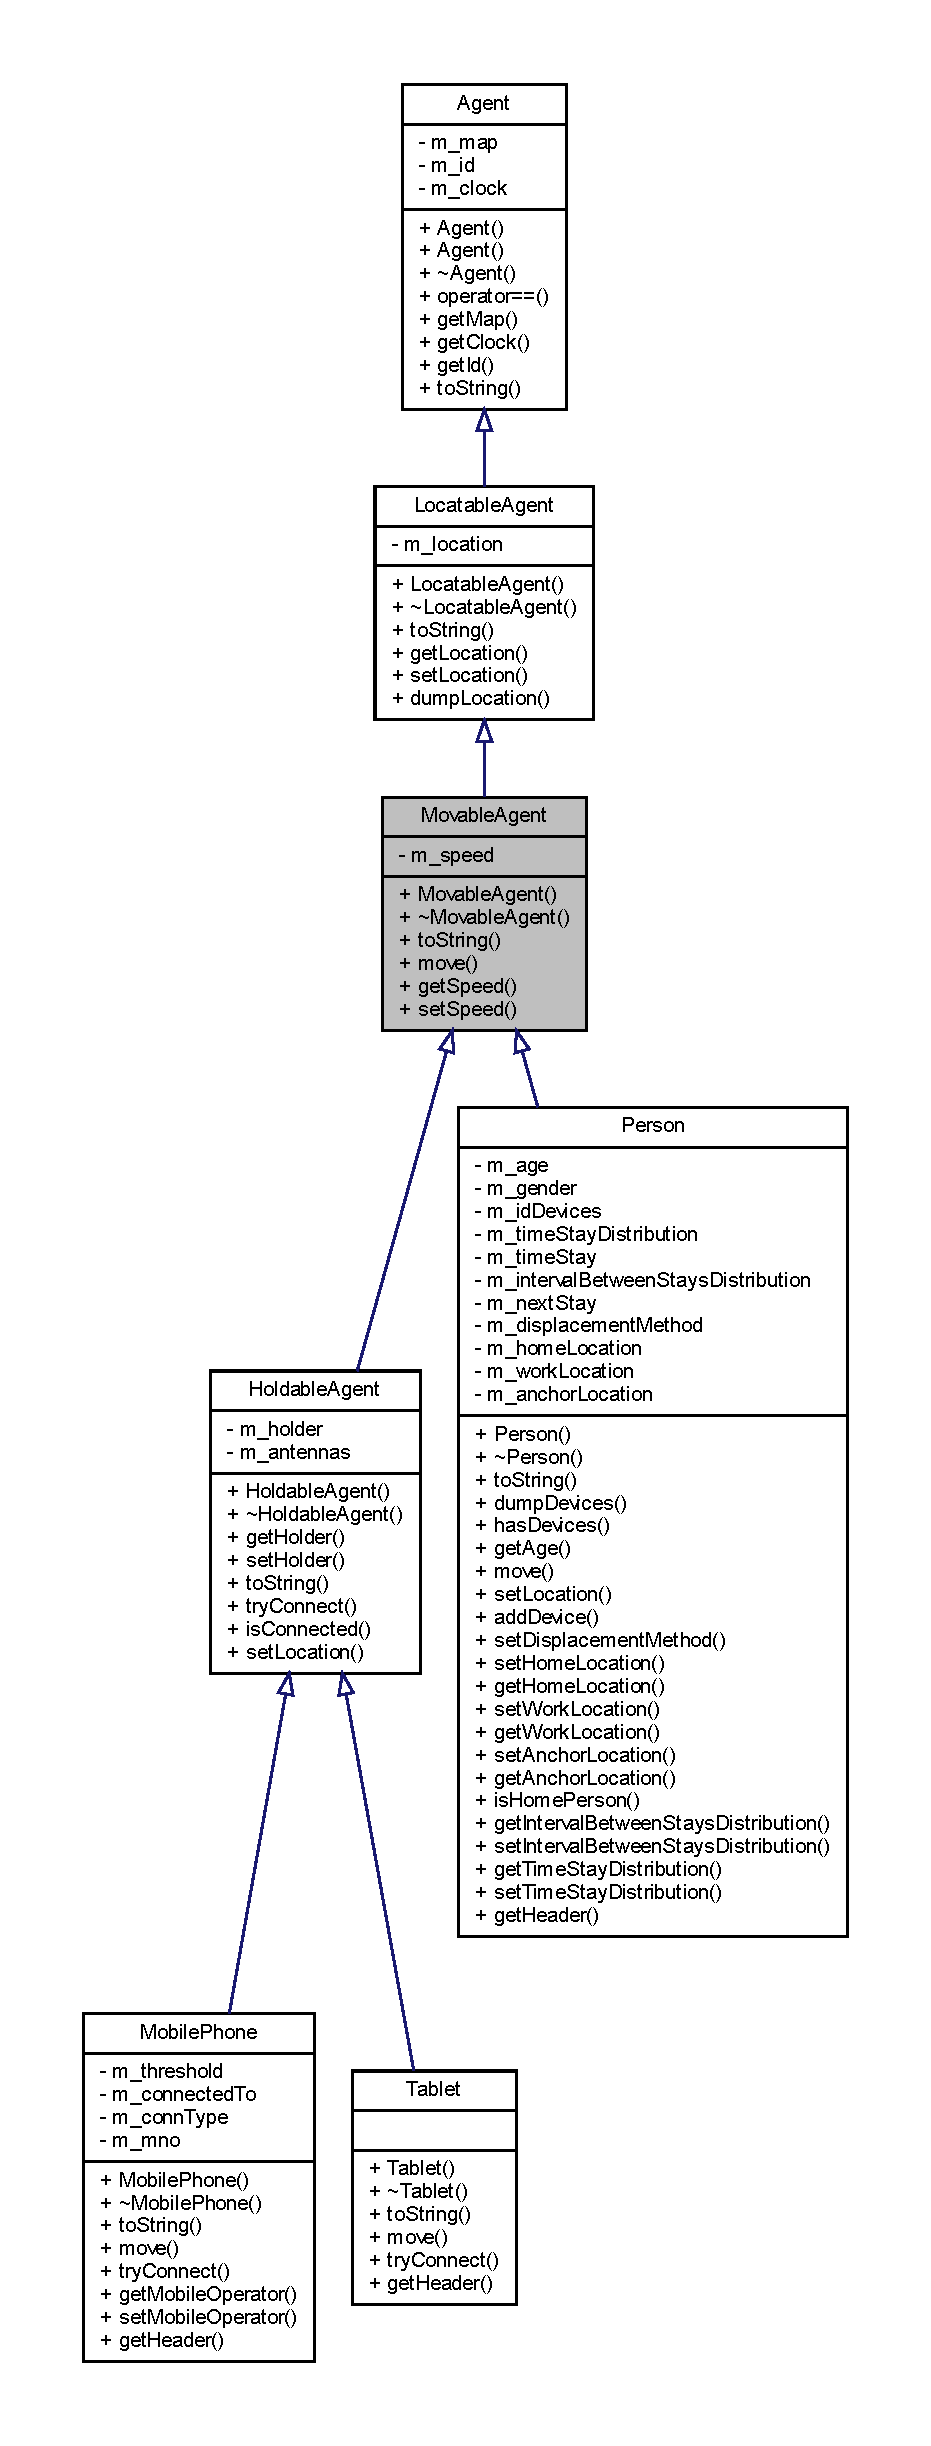
\includegraphics[height=550pt]{class_movable_agent__inherit__graph}
\end{center}
\end{figure}


Collaboration diagram for Movable\+Agent\+:\nopagebreak
\begin{figure}[H]
\begin{center}
\leavevmode
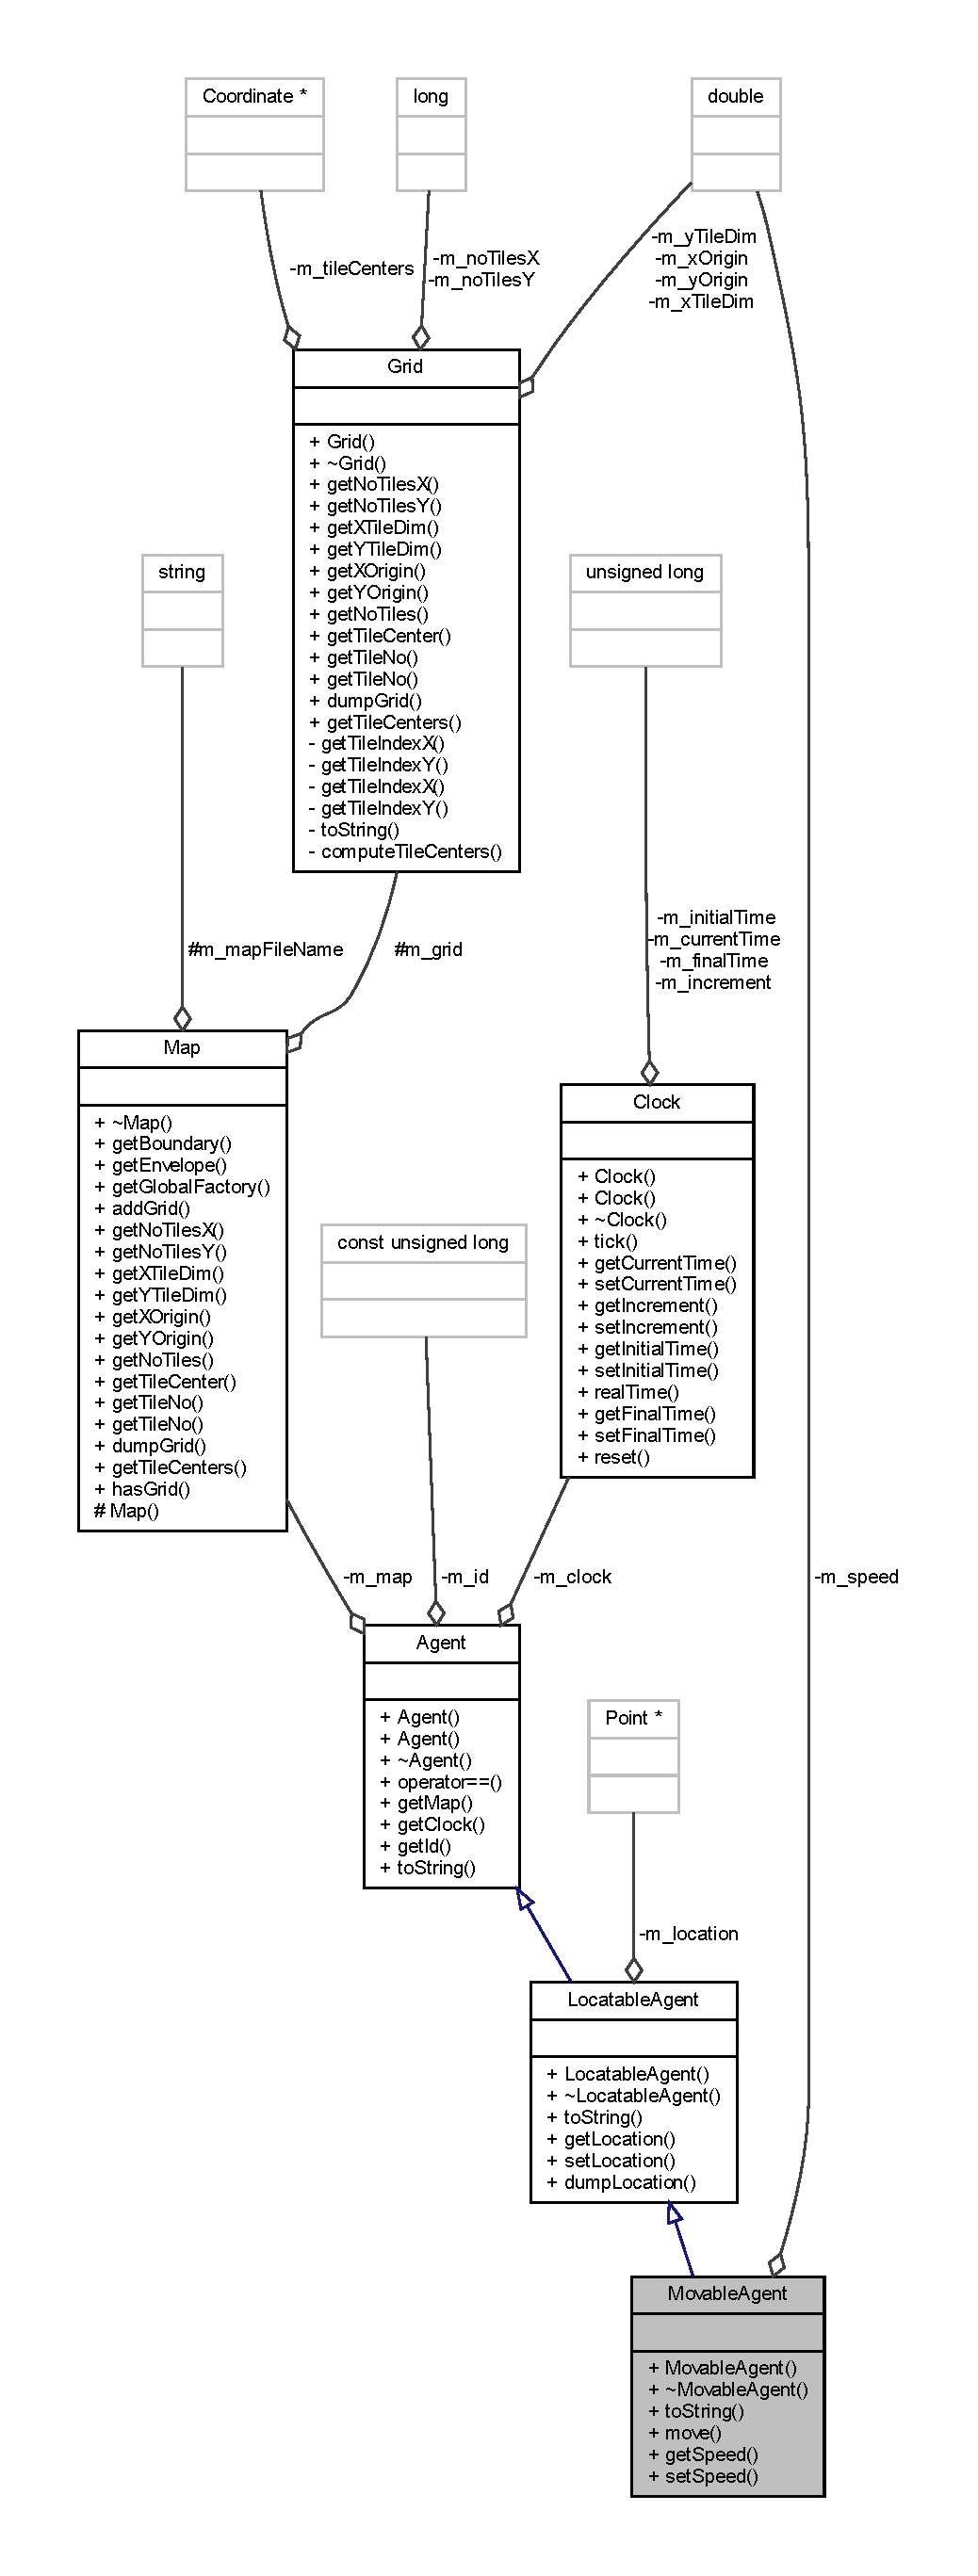
\includegraphics[height=550pt]{class_movable_agent__coll__graph}
\end{center}
\end{figure}
\doxysubsection*{Public Member Functions}
\begin{DoxyCompactItemize}
\item 
\mbox{\hyperlink{class_movable_agent_ad76b14a044181a57ade71f1267a2ccbd}{Movable\+Agent}} (const \mbox{\hyperlink{class_map}{Map}} $\ast$m, const unsigned long id, Point $\ast$init\+Position, const \mbox{\hyperlink{class_clock}{Clock}} $\ast$clock, double init\+Speed)
\item 
virtual \mbox{\hyperlink{class_movable_agent_a20eb9ddcc953137e63e035837918206c}{$\sim$\+Movable\+Agent}} ()
\item 
const string \mbox{\hyperlink{class_movable_agent_a6cd9a1dc9104b5703f74785a87d2c320}{to\+String}} (bool detailed=false) const override
\item 
virtual Point $\ast$ \mbox{\hyperlink{class_movable_agent_a88b617f0e78c817634e5b587da045ab0}{move}} ()=0
\item 
double \mbox{\hyperlink{class_movable_agent_a12fcdaee60f5bb29f15fe113a7dacaac}{get\+Speed}} () const
\item 
void \mbox{\hyperlink{class_movable_agent_ae2ef452e81789a4370e7dee32a9cc67e}{set\+Speed}} (double speed)
\end{DoxyCompactItemize}
\doxysubsection*{Private Attributes}
\begin{DoxyCompactItemize}
\item 
double \mbox{\hyperlink{class_movable_agent_ac725b42e7b968740a59c3e1033d69ac5}{m\+\_\+speed}}
\end{DoxyCompactItemize}


\doxysubsection{Detailed Description}
This class represents an \mbox{\hyperlink{class_agent}{Agent}} that can move on the map. This is an abstract class. It is used as a base class for all agents that can move. Currently only the \mbox{\hyperlink{class_person}{Person}}, \mbox{\hyperlink{class_mobile_phone}{Mobile\+Phone}}, and \mbox{\hyperlink{class_tablet}{Tablet}} classes inherits it and are already implemented. 

\doxysubsection{Constructor \& Destructor Documentation}
\mbox{\Hypertarget{class_movable_agent_ad76b14a044181a57ade71f1267a2ccbd}\label{class_movable_agent_ad76b14a044181a57ade71f1267a2ccbd}} 
\index{MovableAgent@{MovableAgent}!MovableAgent@{MovableAgent}}
\index{MovableAgent@{MovableAgent}!MovableAgent@{MovableAgent}}
\doxysubsubsection{\texorpdfstring{MovableAgent()}{MovableAgent()}}
{\footnotesize\ttfamily Movable\+Agent\+::\+Movable\+Agent (\begin{DoxyParamCaption}\item[{const \mbox{\hyperlink{class_map}{Map}} $\ast$}]{m,  }\item[{const unsigned long}]{id,  }\item[{Point $\ast$}]{init\+Position,  }\item[{const \mbox{\hyperlink{class_clock}{Clock}} $\ast$}]{clock,  }\item[{double}]{init\+Speed }\end{DoxyParamCaption})\hspace{0.3cm}{\ttfamily [explicit]}}

Constructor of the class. 
\begin{DoxyParams}{Parameters}
{\em m} & a pointer to a \mbox{\hyperlink{class_map}{Map}} object used by the simulation. \\
\hline
{\em id} & the id of the object. \\
\hline
{\em init\+Position} & the initial location on the map. \\
\hline
{\em clock} & a pointer to the \mbox{\hyperlink{class_clock}{Clock}} object used by this simulation. \\
\hline
{\em init\+Speed} & the initial speed of the agent. Depending on the derived classes, this value could be read from a configuration file. For example, for the \mbox{\hyperlink{class_person}{Person}} class, this value is specified in the persons configuration file. \\
\hline
\end{DoxyParams}
\mbox{\Hypertarget{class_movable_agent_a20eb9ddcc953137e63e035837918206c}\label{class_movable_agent_a20eb9ddcc953137e63e035837918206c}} 
\index{MovableAgent@{MovableAgent}!````~MovableAgent@{$\sim$MovableAgent}}
\index{````~MovableAgent@{$\sim$MovableAgent}!MovableAgent@{MovableAgent}}
\doxysubsubsection{\texorpdfstring{$\sim$MovableAgent()}{~MovableAgent()}}
{\footnotesize\ttfamily virtual Movable\+Agent\+::$\sim$\+Movable\+Agent (\begin{DoxyParamCaption}{ }\end{DoxyParamCaption})\hspace{0.3cm}{\ttfamily [virtual]}}

The default destructor. 

\doxysubsection{Member Function Documentation}
\mbox{\Hypertarget{class_movable_agent_a12fcdaee60f5bb29f15fe113a7dacaac}\label{class_movable_agent_a12fcdaee60f5bb29f15fe113a7dacaac}} 
\index{MovableAgent@{MovableAgent}!getSpeed@{getSpeed}}
\index{getSpeed@{getSpeed}!MovableAgent@{MovableAgent}}
\doxysubsubsection{\texorpdfstring{getSpeed()}{getSpeed()}}
{\footnotesize\ttfamily double Movable\+Agent\+::get\+Speed (\begin{DoxyParamCaption}{ }\end{DoxyParamCaption}) const}

Returns the speed of this agent. \begin{DoxyReturn}{Returns}
the speed of this agent. 
\end{DoxyReturn}
\mbox{\Hypertarget{class_movable_agent_a88b617f0e78c817634e5b587da045ab0}\label{class_movable_agent_a88b617f0e78c817634e5b587da045ab0}} 
\index{MovableAgent@{MovableAgent}!move@{move}}
\index{move@{move}!MovableAgent@{MovableAgent}}
\doxysubsubsection{\texorpdfstring{move()}{move()}}
{\footnotesize\ttfamily virtual Point$\ast$ Movable\+Agent\+::move (\begin{DoxyParamCaption}{ }\end{DoxyParamCaption})\hspace{0.3cm}{\ttfamily [pure virtual]}}

A pure virtual method used to move the agent to a new location on the map. All the classes that inherit \mbox{\hyperlink{class_movable_agent}{Movable\+Agent}} implement this function. The actual implementation is based on a Strategy design pattern. \mbox{\hyperlink{class_displace}{Displace}} class defines the displacement strategy interface and the classes that inherits it implements the interface defining concrete displacement methods. \begin{DoxyReturn}{Returns}
the final location after displacement. 
\end{DoxyReturn}


Implemented in \mbox{\hyperlink{class_person_a922e0462a1e7eac6523a9a864ce27afc}{Person}}, \mbox{\hyperlink{class_mobile_phone_a785d0cac08252386603c702ad8f38c5b}{Mobile\+Phone}}, and \mbox{\hyperlink{class_tablet_ab1b8c7591be0c6ea118c8ab1c17839bb}{Tablet}}.

\mbox{\Hypertarget{class_movable_agent_ae2ef452e81789a4370e7dee32a9cc67e}\label{class_movable_agent_ae2ef452e81789a4370e7dee32a9cc67e}} 
\index{MovableAgent@{MovableAgent}!setSpeed@{setSpeed}}
\index{setSpeed@{setSpeed}!MovableAgent@{MovableAgent}}
\doxysubsubsection{\texorpdfstring{setSpeed()}{setSpeed()}}
{\footnotesize\ttfamily void Movable\+Agent\+::set\+Speed (\begin{DoxyParamCaption}\item[{double}]{speed }\end{DoxyParamCaption})}

Sets the speed of this agent. 
\begin{DoxyParams}{Parameters}
{\em speed} & the speed of this agent. \\
\hline
\end{DoxyParams}
\mbox{\Hypertarget{class_movable_agent_a6cd9a1dc9104b5703f74785a87d2c320}\label{class_movable_agent_a6cd9a1dc9104b5703f74785a87d2c320}} 
\index{MovableAgent@{MovableAgent}!toString@{toString}}
\index{toString@{toString}!MovableAgent@{MovableAgent}}
\doxysubsubsection{\texorpdfstring{toString()}{toString()}}
{\footnotesize\ttfamily const string Movable\+Agent\+::to\+String (\begin{DoxyParamCaption}\item[{bool}]{detailed = {\ttfamily false} }\end{DoxyParamCaption}) const\hspace{0.3cm}{\ttfamily [override]}, {\ttfamily [virtual]}}

Builds a string with the most relevant information of the class. It is useful to output the description of concrete agents to the console or to a file. Currently, the value of the {\ttfamily detailed} parameter is ignored. 
\begin{DoxyParams}{Parameters}
{\em detailed} & the value of this parameter is ignored. \\
\hline
\end{DoxyParams}
\begin{DoxyReturn}{Returns}
a string object containing the id, the coordinates of the location of the agent and the initial speed of movement. 
\end{DoxyReturn}


Reimplemented from \mbox{\hyperlink{class_locatable_agent_ac3761e9b566f8ddcd1a663fcbf97eeac}{Locatable\+Agent}}.



Reimplemented in \mbox{\hyperlink{class_person_a3c38c40dab5c071d20fe3aaab51975a2}{Person}}, and \mbox{\hyperlink{class_tablet_aae4c82133cbf3e7d7e8c0cca11925159}{Tablet}}.



\doxysubsection{Member Data Documentation}
\mbox{\Hypertarget{class_movable_agent_ac725b42e7b968740a59c3e1033d69ac5}\label{class_movable_agent_ac725b42e7b968740a59c3e1033d69ac5}} 
\index{MovableAgent@{MovableAgent}!m\_speed@{m\_speed}}
\index{m\_speed@{m\_speed}!MovableAgent@{MovableAgent}}
\doxysubsubsection{\texorpdfstring{m\_speed}{m\_speed}}
{\footnotesize\ttfamily double Movable\+Agent\+::m\+\_\+speed\hspace{0.3cm}{\ttfamily [private]}}



The documentation for this class was generated from the following file\+:\begin{DoxyCompactItemize}
\item 
include/agent/\mbox{\hyperlink{_movable_agent_8h}{Movable\+Agent.\+h}}\end{DoxyCompactItemize}

\hypertarget{class_net_prior_post_loc_prob}{}\doxysection{Net\+Prior\+Post\+Loc\+Prob Class Reference}
\label{class_net_prior_post_loc_prob}\index{NetPriorPostLocProb@{NetPriorPostLocProb}}


{\ttfamily \#include $<$Net\+Prior\+Post\+Loc\+Prob.\+h$>$}



Inheritance diagram for Net\+Prior\+Post\+Loc\+Prob\+:\nopagebreak
\begin{figure}[H]
\begin{center}
\leavevmode
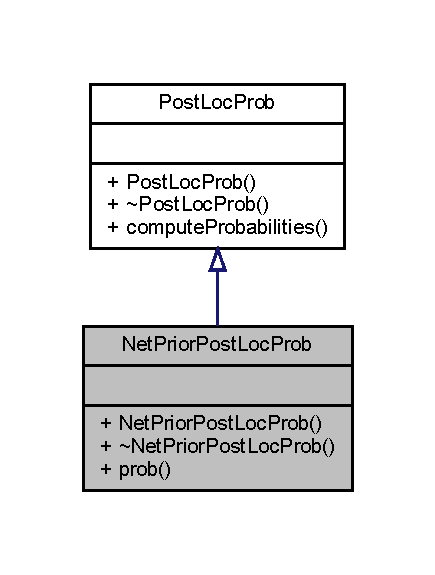
\includegraphics[width=209pt]{class_net_prior_post_loc_prob__inherit__graph}
\end{center}
\end{figure}


Collaboration diagram for Net\+Prior\+Post\+Loc\+Prob\+:\nopagebreak
\begin{figure}[H]
\begin{center}
\leavevmode
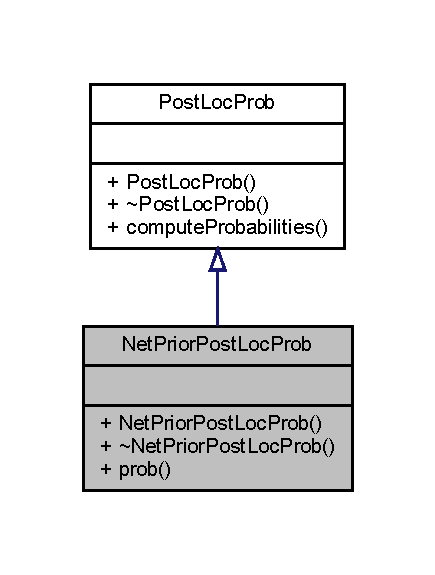
\includegraphics[width=209pt]{class_net_prior_post_loc_prob__coll__graph}
\end{center}
\end{figure}
\doxysubsection*{Public Member Functions}
\begin{DoxyCompactItemize}
\item 
\mbox{\hyperlink{class_net_prior_post_loc_prob_af004c0a058e1bfbefb96ec5d50c7c67e}{Net\+Prior\+Post\+Loc\+Prob}} (const \mbox{\hyperlink{class_map}{Map}} $\ast$m, \mbox{\hyperlink{class_clock}{Clock}} $\ast$clk, \mbox{\hyperlink{class_agents_collection}{Agents\+Collection}} $\ast$agents, map$<$ const unsigned long, const string $>$ prob\+Files)
\item 
virtual \mbox{\hyperlink{class_net_prior_post_loc_prob_a08097bd70b7d1020484971279c31acb2}{$\sim$\+Net\+Prior\+Post\+Loc\+Prob}} ()
\item 
virtual vector$<$ double $>$ \mbox{\hyperlink{class_net_prior_post_loc_prob_ae641d8868b315caa0ab26e36072f381a}{prob}} (unsigned long t, \mbox{\hyperlink{class_mobile_phone}{Mobile\+Phone}} $\ast$m, vector$<$ \mbox{\hyperlink{class_antenna_info}{Antenna\+Info}} $>$ \&data, pair$<$ \mbox{\hyperlink{_agents_collection_8h_afde47bc45d604b8b8c72755072376679}{um\+\_\+iterator}}, \mbox{\hyperlink{_agents_collection_8h_afde47bc45d604b8b8c72755072376679}{um\+\_\+iterator}} $>$ it) override
\end{DoxyCompactItemize}


\doxysubsection{Constructor \& Destructor Documentation}
\mbox{\Hypertarget{class_net_prior_post_loc_prob_af004c0a058e1bfbefb96ec5d50c7c67e}\label{class_net_prior_post_loc_prob_af004c0a058e1bfbefb96ec5d50c7c67e}} 
\index{NetPriorPostLocProb@{NetPriorPostLocProb}!NetPriorPostLocProb@{NetPriorPostLocProb}}
\index{NetPriorPostLocProb@{NetPriorPostLocProb}!NetPriorPostLocProb@{NetPriorPostLocProb}}
\doxysubsubsection{\texorpdfstring{NetPriorPostLocProb()}{NetPriorPostLocProb()}}
{\footnotesize\ttfamily Net\+Prior\+Post\+Loc\+Prob\+::\+Net\+Prior\+Post\+Loc\+Prob (\begin{DoxyParamCaption}\item[{const \mbox{\hyperlink{class_map}{Map}} $\ast$}]{m,  }\item[{\mbox{\hyperlink{class_clock}{Clock}} $\ast$}]{clk,  }\item[{\mbox{\hyperlink{class_agents_collection}{Agents\+Collection}} $\ast$}]{agents,  }\item[{map$<$ const unsigned long, const string $>$}]{prob\+Files }\end{DoxyParamCaption})}

Constructor of the class. It sets the members according to the values given as parameters. 
\begin{DoxyParams}{Parameters}
{\em m} & a pointer to the \mbox{\hyperlink{class_map}{Map}} object of the simulation. \\
\hline
{\em clk} & a pointer to the \mbox{\hyperlink{class_clock}{Clock}} object of the simulation. \\
\hline
{\em agents} & a pointer to the \mbox{\hyperlink{class_agents_collection}{Agents\+Collection}} object. \\
\hline
{\em prob\+Files} & the name of the files where the posterior probabilities are saved (one file per M\+NO). \\
\hline
\end{DoxyParams}
\mbox{\Hypertarget{class_net_prior_post_loc_prob_a08097bd70b7d1020484971279c31acb2}\label{class_net_prior_post_loc_prob_a08097bd70b7d1020484971279c31acb2}} 
\index{NetPriorPostLocProb@{NetPriorPostLocProb}!````~NetPriorPostLocProb@{$\sim$NetPriorPostLocProb}}
\index{````~NetPriorPostLocProb@{$\sim$NetPriorPostLocProb}!NetPriorPostLocProb@{NetPriorPostLocProb}}
\doxysubsubsection{\texorpdfstring{$\sim$NetPriorPostLocProb()}{~NetPriorPostLocProb()}}
{\footnotesize\ttfamily virtual Net\+Prior\+Post\+Loc\+Prob\+::$\sim$\+Net\+Prior\+Post\+Loc\+Prob (\begin{DoxyParamCaption}{ }\end{DoxyParamCaption})\hspace{0.3cm}{\ttfamily [virtual]}}

Default destructor 

\doxysubsection{Member Function Documentation}
\mbox{\Hypertarget{class_net_prior_post_loc_prob_ae641d8868b315caa0ab26e36072f381a}\label{class_net_prior_post_loc_prob_ae641d8868b315caa0ab26e36072f381a}} 
\index{NetPriorPostLocProb@{NetPriorPostLocProb}!prob@{prob}}
\index{prob@{prob}!NetPriorPostLocProb@{NetPriorPostLocProb}}
\doxysubsubsection{\texorpdfstring{prob()}{prob()}}
{\footnotesize\ttfamily virtual vector$<$double$>$ Net\+Prior\+Post\+Loc\+Prob\+::prob (\begin{DoxyParamCaption}\item[{unsigned long}]{t,  }\item[{\mbox{\hyperlink{class_mobile_phone}{Mobile\+Phone}} $\ast$}]{m,  }\item[{vector$<$ \mbox{\hyperlink{class_antenna_info}{Antenna\+Info}} $>$ \&}]{data,  }\item[{pair$<$ \mbox{\hyperlink{_agents_collection_8h_afde47bc45d604b8b8c72755072376679}{um\+\_\+iterator}}, \mbox{\hyperlink{_agents_collection_8h_afde47bc45d604b8b8c72755072376679}{um\+\_\+iterator}} $>$}]{it }\end{DoxyParamCaption})\hspace{0.3cm}{\ttfamily [override]}, {\ttfamily [virtual]}}

Implements the computation of the posterior location probabilities with the prior probabilities given by the network. 
\begin{DoxyParams}{Parameters}
{\em t} & the time instant for which the probabilities are computed. \\
\hline
{\em m} & a pointer to a \mbox{\hyperlink{class_mobile_phone}{Mobile\+Phone}} object for which the probabilities are computed. \\
\hline
{\em data} & a vector with the network events. \\
\hline
{\em it} & an iterator the the antenna\textquotesingle{}s list. \\
\hline
\end{DoxyParams}
\begin{DoxyReturn}{Returns}
a vector with the posterior location probabilities for each time instant and mobile phone. 
\end{DoxyReturn}


The documentation for this class was generated from the following file\+:\begin{DoxyCompactItemize}
\item 
include/\mbox{\hyperlink{_net_prior_post_loc_prob_8h}{Net\+Prior\+Post\+Loc\+Prob.\+h}}\end{DoxyCompactItemize}

\hypertarget{class_person}{}\doxysection{Person Class Reference}
\label{class_person}\index{Person@{Person}}


{\ttfamily \#include $<$Person.\+h$>$}



Inheritance diagram for Person\+:\nopagebreak
\begin{figure}[H]
\begin{center}
\leavevmode
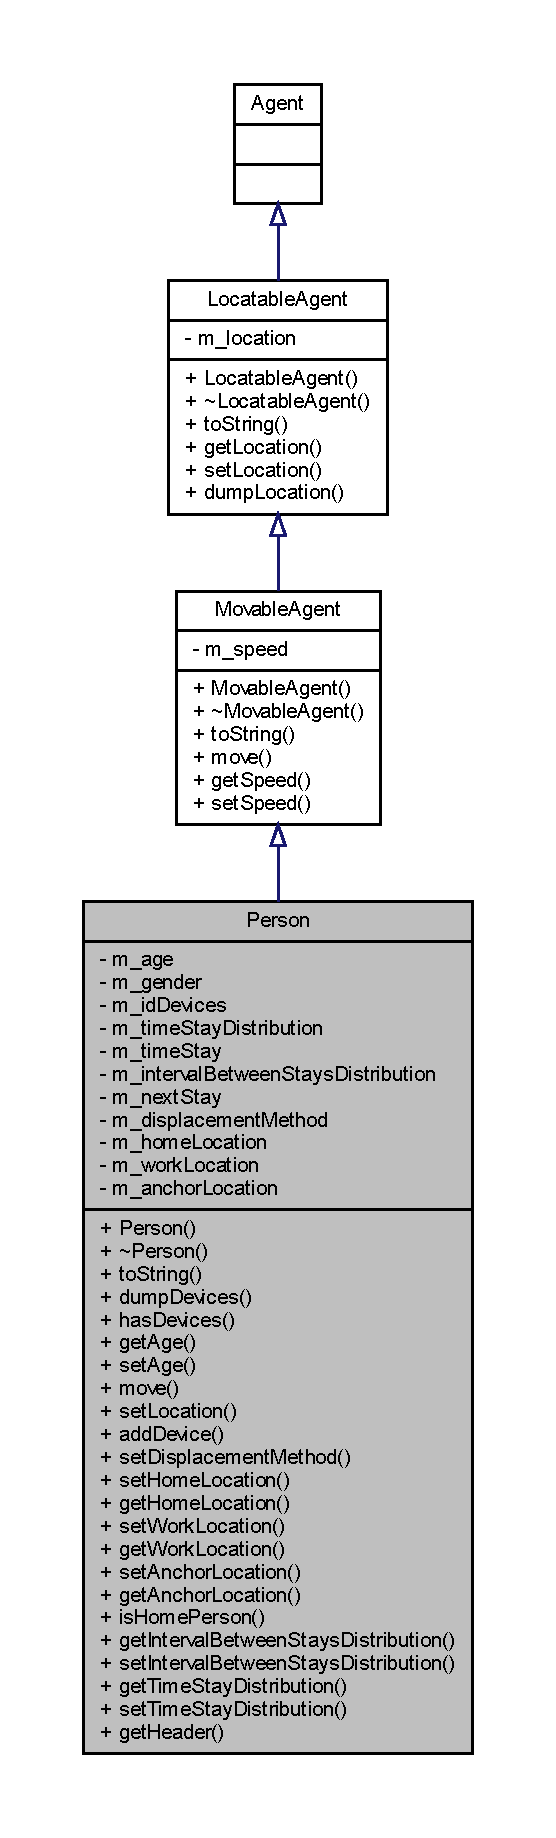
\includegraphics[height=550pt]{class_person__inherit__graph}
\end{center}
\end{figure}


Collaboration diagram for Person\+:\nopagebreak
\begin{figure}[H]
\begin{center}
\leavevmode
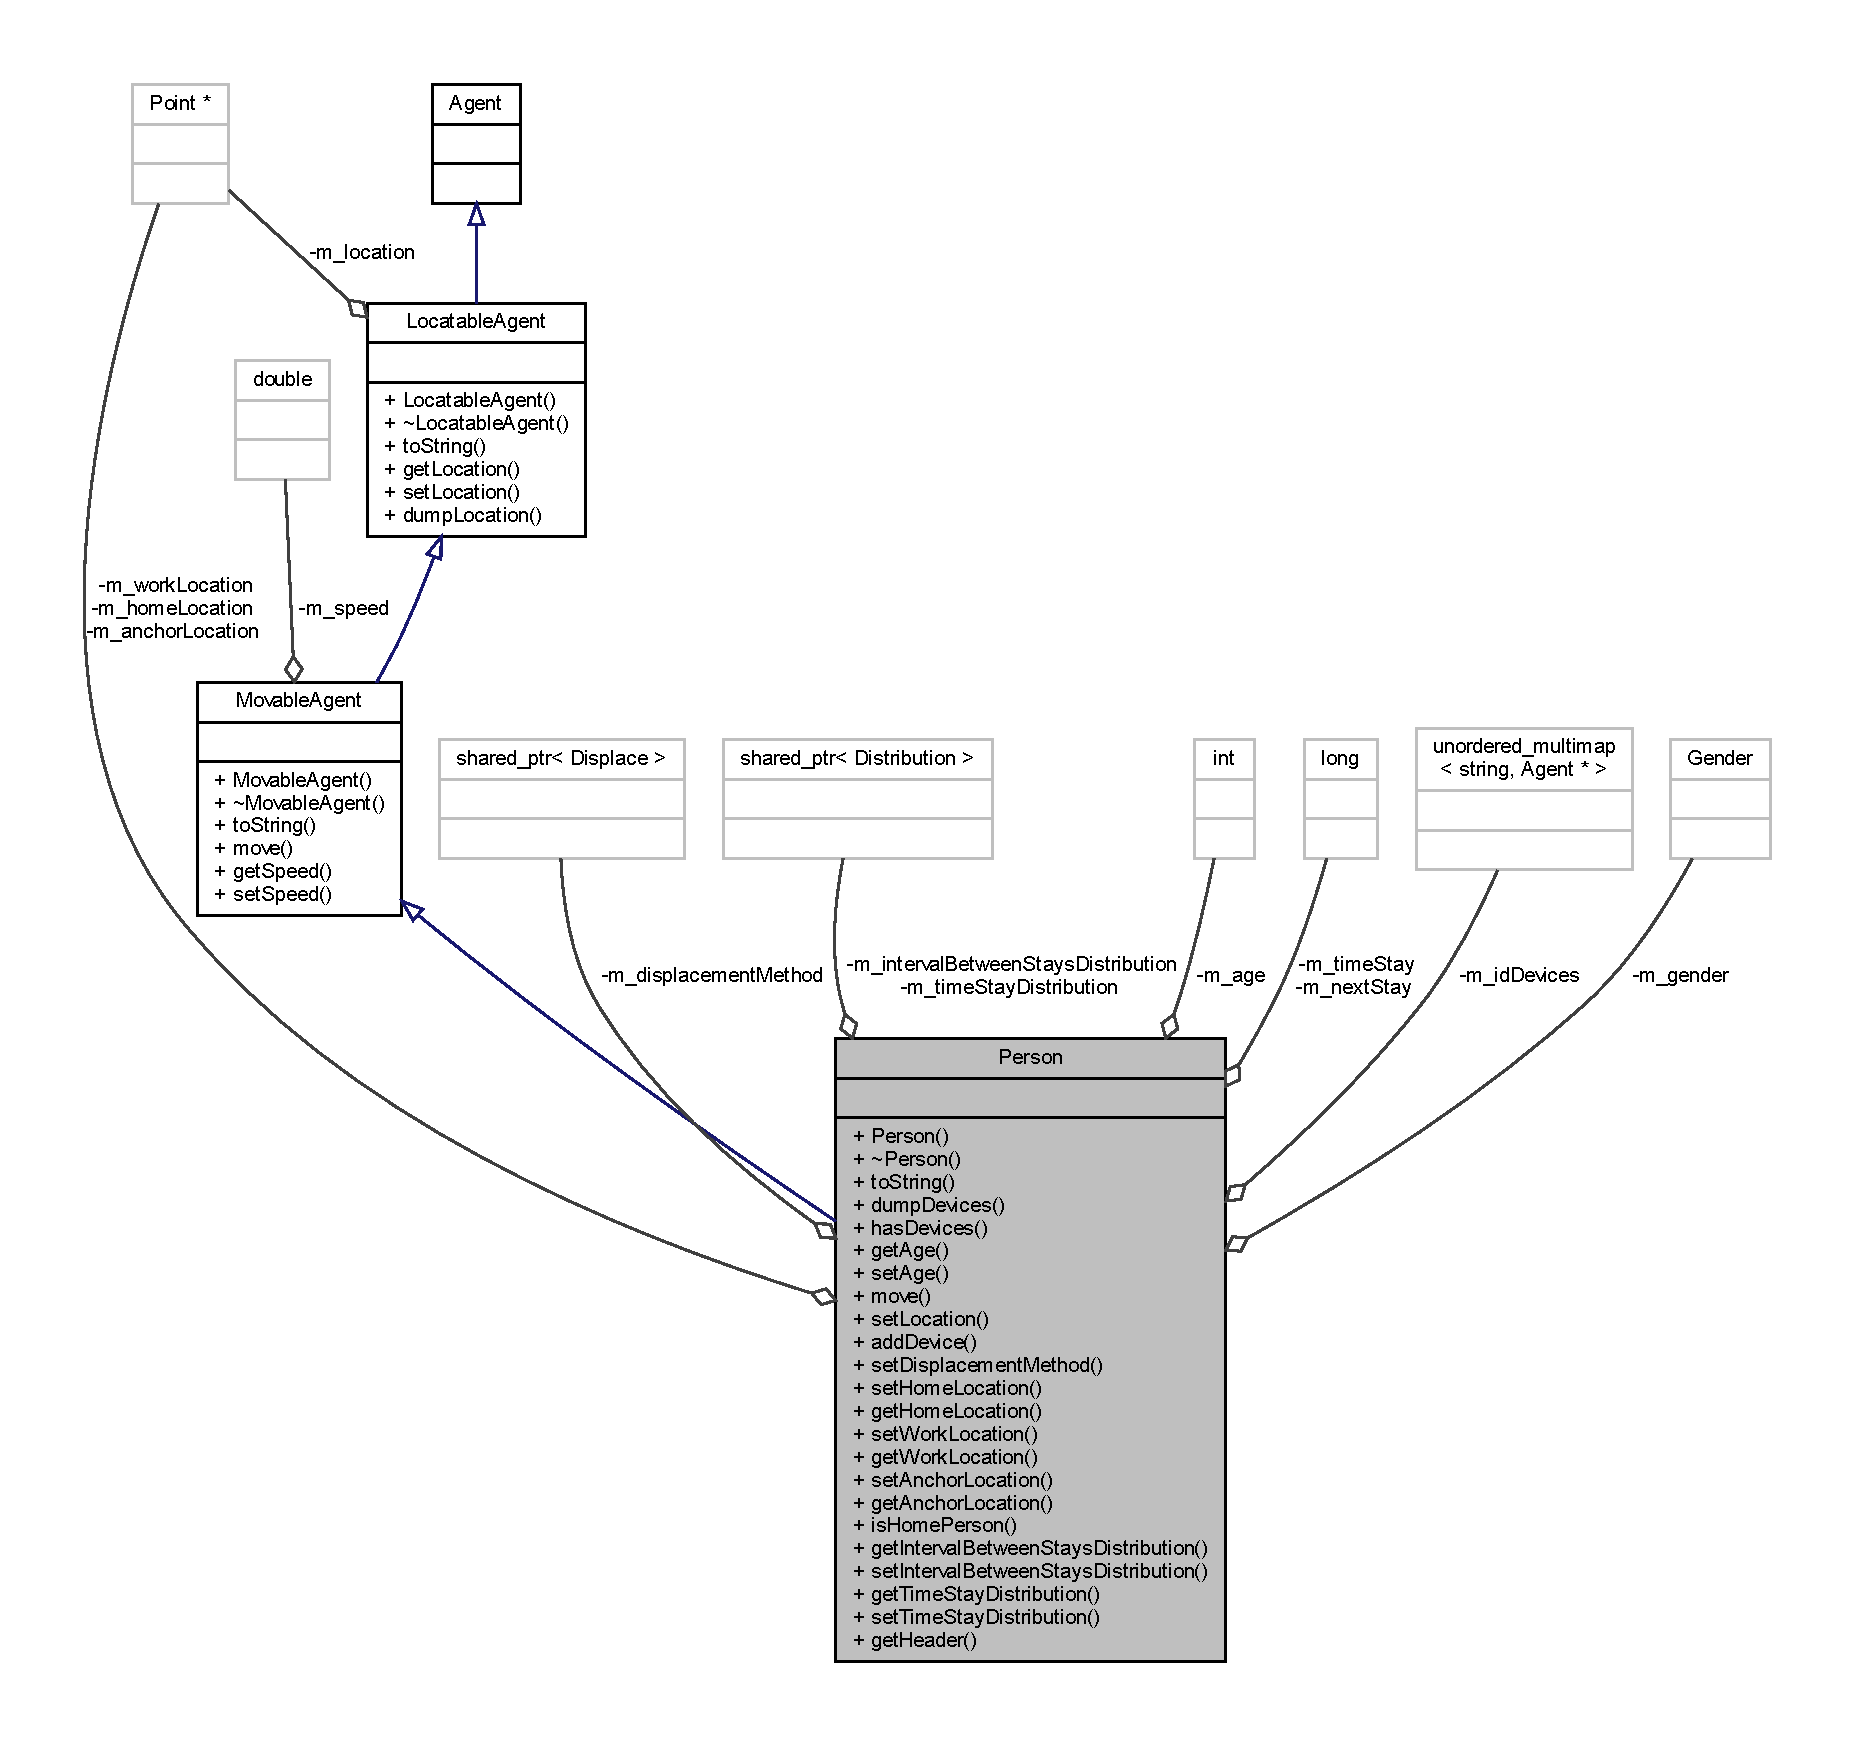
\includegraphics[width=350pt]{class_person__coll__graph}
\end{center}
\end{figure}
\doxysubsection*{Public Types}
\begin{DoxyCompactItemize}
\item 
enum \mbox{\hyperlink{class_person_aff84ca16bd4dbf364614d86f20b29dd2}{Gender}} \{ \mbox{\hyperlink{class_person_aff84ca16bd4dbf364614d86f20b29dd2a16691f7cc6595f87b71d9b43ad23fcb4}{M\+A\+LE}}, 
\mbox{\hyperlink{class_person_aff84ca16bd4dbf364614d86f20b29dd2a8ee21010fb2d8e8794ef72be368da064}{F\+E\+M\+A\+LE}}
 \}
\end{DoxyCompactItemize}
\doxysubsection*{Public Member Functions}
\begin{DoxyCompactItemize}
\item 
\mbox{\hyperlink{class_person_afe423944473e3eb5b52f30ee2a084f71}{Person}} (const \mbox{\hyperlink{class_map}{Map}} $\ast$m, const unsigned long id, Point $\ast$init\+Position, const \mbox{\hyperlink{class_clock}{Clock}} $\ast$clock, double init\+Speed, int age, \mbox{\hyperlink{class_person_aff84ca16bd4dbf364614d86f20b29dd2}{Gender}} gender, shared\+\_\+ptr$<$ \mbox{\hyperlink{class_distribution}{Distribution}} $>$ time\+Stay\+Distribution, shared\+\_\+ptr$<$ \mbox{\hyperlink{class_distribution}{Distribution}} $>$ interval\+Between\+Stays\+Distribution)
\item 
virtual \mbox{\hyperlink{class_person_a6b5729bb56531c93312b1179c8ee4b71}{$\sim$\+Person}} ()
\item 
const string \mbox{\hyperlink{class_person_a3c38c40dab5c071d20fe3aaab51975a2}{to\+String}} (bool detailed=false) const override
\item 
string \mbox{\hyperlink{class_person_a0bc06f77b3e8a151f8c5cc77459895c9}{dump\+Devices}} ()
\item 
bool \mbox{\hyperlink{class_person_a40d6f2c716dd3c9794067817a3fb9165}{has\+Devices}} ()
\item 
int \mbox{\hyperlink{class_person_a4b66dbee570398920b8fb6aacddd2559}{get\+Age}} () const
\item 
virtual Point $\ast$ \mbox{\hyperlink{class_person_a922e0462a1e7eac6523a9a864ce27afc}{move}} () override
\item 
virtual void \mbox{\hyperlink{class_person_a05f4ac2107d59e03f0f336eda08aa358}{set\+Location}} (Point $\ast$pt) override
\item 
void \mbox{\hyperlink{class_person_a3ce0a72a98c2e723e48dcd7b4d9af599}{add\+Device}} (string type, \mbox{\hyperlink{class_agent}{Agent}} $\ast$agent)
\item 
void \mbox{\hyperlink{class_person_a89ada26d3541bc82e514dae833dc959d}{set\+Displacement\+Method}} (const shared\+\_\+ptr$<$ \mbox{\hyperlink{class_displace}{Displace}} $>$ \&displace)
\item 
void \mbox{\hyperlink{class_person_adec201127069d8641b1a9c631982e2b5}{set\+Home\+Location}} (Point $\ast$hl)
\item 
Point $\ast$ \mbox{\hyperlink{class_person_aec5061097976b57412964fcfc203a0a4}{get\+Home\+Location}} () const
\item 
void \mbox{\hyperlink{class_person_a2dcf5c090e1191096497a716dde1e5b9}{set\+Work\+Location}} (Point $\ast$wl)
\item 
Point $\ast$ \mbox{\hyperlink{class_person_a52647a49c2efde4983dfb1667227cad6}{get\+Work\+Location}} () const
\item 
void \mbox{\hyperlink{class_person_a872e8a5ac7610d5b518323338d5c6e6f}{set\+Anchor\+Location}} (Point $\ast$al)
\item 
Point $\ast$ \mbox{\hyperlink{class_person_a3ead25787039169027f392f09122a33b}{get\+Anchor\+Location}} () const
\item 
bool \mbox{\hyperlink{class_person_a7c14f732bc1bf8fa981906ee505300a5}{is\+Home\+Person}} () const
\item 
const shared\+\_\+ptr$<$ \mbox{\hyperlink{class_distribution}{Distribution}} $>$ \& \mbox{\hyperlink{class_person_ad8d03204dc96ac5eb03042be33ffcac9}{get\+Interval\+Between\+Stays\+Distribution}} () const
\item 
void \mbox{\hyperlink{class_person_a0ee6d8c78f596a3dbe7ce3013772864a}{set\+Interval\+Between\+Stays\+Distribution}} (const shared\+\_\+ptr$<$ \mbox{\hyperlink{class_distribution}{Distribution}} $>$ \&interval\+Between\+Stays\+Distribution)
\item 
const shared\+\_\+ptr$<$ \mbox{\hyperlink{class_distribution}{Distribution}} $>$ \& \mbox{\hyperlink{class_person_a3d0731eb8962e17c815a3b480b6b44e1}{get\+Time\+Stay\+Distribution}} () const
\item 
void \mbox{\hyperlink{class_person_a2a920bf3a1e90355f393b5f4d0c14a7c}{set\+Time\+Stay\+Distribution}} (const shared\+\_\+ptr$<$ \mbox{\hyperlink{class_distribution}{Distribution}} $>$ \&time\+Stay\+Distribution)
\end{DoxyCompactItemize}
\doxysubsection*{Static Public Member Functions}
\begin{DoxyCompactItemize}
\item 
static const string \mbox{\hyperlink{class_person_a6bebe59c354f26f4cb983185d6084181}{get\+Header}} ()
\end{DoxyCompactItemize}
\doxysubsection*{Private Attributes}
\begin{DoxyCompactItemize}
\item 
int \mbox{\hyperlink{class_person_a743e071da10a5ac9150f61df919cfbb4}{m\+\_\+age}}
\item 
\mbox{\hyperlink{class_person_aff84ca16bd4dbf364614d86f20b29dd2}{Gender}} \mbox{\hyperlink{class_person_ade9cdf49acde95c75f19f0b0d24c8c9a}{m\+\_\+gender}}
\item 
unordered\+\_\+multimap$<$ string, \mbox{\hyperlink{class_agent}{Agent}} $\ast$ $>$ \mbox{\hyperlink{class_person_a95b2e60a54b72aea51a7600048e76291}{m\+\_\+id\+Devices}}
\item 
shared\+\_\+ptr$<$ \mbox{\hyperlink{class_distribution}{Distribution}} $>$ \mbox{\hyperlink{class_person_a20c309fb76477a0040c61e8fb1ab55d2}{m\+\_\+time\+Stay\+Distribution}}
\item 
unsigned long \mbox{\hyperlink{class_person_a5554109f1f3a7c466f02346d0061c6e7}{m\+\_\+time\+Stay}}
\item 
shared\+\_\+ptr$<$ \mbox{\hyperlink{class_distribution}{Distribution}} $>$ \mbox{\hyperlink{class_person_a7fe9a2ce5b7cbebcfcc4a2f15acecd01}{m\+\_\+interval\+Between\+Stays\+Distribution}}
\item 
unsigned long \mbox{\hyperlink{class_person_ad8809184fc32b28b1bcc115b10493b55}{m\+\_\+next\+Stay}}
\item 
shared\+\_\+ptr$<$ \mbox{\hyperlink{class_displace}{Displace}} $>$ \mbox{\hyperlink{class_person_a92ceead10a7ca858d2151391e4421843}{m\+\_\+displacement\+Method}}
\item 
Point $\ast$ \mbox{\hyperlink{class_person_a9137e6d5f054e53799c66d354d403711}{m\+\_\+home\+Location}}
\item 
Point $\ast$ \mbox{\hyperlink{class_person_aa8cf5339fd9eec3cb584d35f4faf8e5f}{m\+\_\+work\+Location}}
\item 
Point $\ast$ \mbox{\hyperlink{class_person_a6c18c99510c569a00c301447771e7388}{m\+\_\+anchor\+Location}}
\end{DoxyCompactItemize}


\doxysubsection{Detailed Description}
This class represents a person that can have 0, 1 or 2 mobile phone(s). During the simulation, the person move around the map, carrying his/her mobile device(s). At every time step, a new location is computed according to a movement strategy. 

\doxysubsection{Member Enumeration Documentation}
\mbox{\Hypertarget{class_person_aff84ca16bd4dbf364614d86f20b29dd2}\label{class_person_aff84ca16bd4dbf364614d86f20b29dd2}} 
\index{Person@{Person}!Gender@{Gender}}
\index{Gender@{Gender}!Person@{Person}}
\doxysubsubsection{\texorpdfstring{Gender}{Gender}}
{\footnotesize\ttfamily enum \mbox{\hyperlink{class_person_aff84ca16bd4dbf364614d86f20b29dd2}{Person\+::\+Gender}}}

\begin{DoxyEnumFields}{Enumerator}
\raisebox{\heightof{T}}[0pt][0pt]{\index{MALE@{MALE}!Person@{Person}}\index{Person@{Person}!MALE@{MALE}}}\mbox{\Hypertarget{class_person_aff84ca16bd4dbf364614d86f20b29dd2a16691f7cc6595f87b71d9b43ad23fcb4}\label{class_person_aff84ca16bd4dbf364614d86f20b29dd2a16691f7cc6595f87b71d9b43ad23fcb4}} 
M\+A\+LE&\\
\hline

\raisebox{\heightof{T}}[0pt][0pt]{\index{FEMALE@{FEMALE}!Person@{Person}}\index{Person@{Person}!FEMALE@{FEMALE}}}\mbox{\Hypertarget{class_person_aff84ca16bd4dbf364614d86f20b29dd2a8ee21010fb2d8e8794ef72be368da064}\label{class_person_aff84ca16bd4dbf364614d86f20b29dd2a8ee21010fb2d8e8794ef72be368da064}} 
F\+E\+M\+A\+LE&\\
\hline

\end{DoxyEnumFields}


\doxysubsection{Constructor \& Destructor Documentation}
\mbox{\Hypertarget{class_person_afe423944473e3eb5b52f30ee2a084f71}\label{class_person_afe423944473e3eb5b52f30ee2a084f71}} 
\index{Person@{Person}!Person@{Person}}
\index{Person@{Person}!Person@{Person}}
\doxysubsubsection{\texorpdfstring{Person()}{Person()}}
{\footnotesize\ttfamily Person\+::\+Person (\begin{DoxyParamCaption}\item[{const \mbox{\hyperlink{class_map}{Map}} $\ast$}]{m,  }\item[{const unsigned long}]{id,  }\item[{Point $\ast$}]{init\+Position,  }\item[{const \mbox{\hyperlink{class_clock}{Clock}} $\ast$}]{clock,  }\item[{double}]{init\+Speed,  }\item[{int}]{age,  }\item[{\mbox{\hyperlink{class_person_aff84ca16bd4dbf364614d86f20b29dd2}{Gender}}}]{gender,  }\item[{shared\+\_\+ptr$<$ \mbox{\hyperlink{class_distribution}{Distribution}} $>$}]{time\+Stay\+Distribution,  }\item[{shared\+\_\+ptr$<$ \mbox{\hyperlink{class_distribution}{Distribution}} $>$}]{interval\+Between\+Stays\+Distribution }\end{DoxyParamCaption})\hspace{0.3cm}{\ttfamily [explicit]}}

Builds a new \mbox{\hyperlink{class_person}{Person}} object with the characteristics given as parameters. 
\begin{DoxyParams}{Parameters}
{\em m} & a pointer to the \mbox{\hyperlink{class_map}{Map}} object where this \mbox{\hyperlink{class_person}{Person}} move. \\
\hline
{\em id} & the id of the \mbox{\hyperlink{class_person}{Person}} object. \\
\hline
{\em init\+Position} & the initial location of the person on the map. \\
\hline
{\em clock} & a pointer to a \mbox{\hyperlink{class_clock}{Clock}} object used for this simulation. \\
\hline
{\em init\+Speed} & the initial speed of this person. It is provided in the configuration file. \\
\hline
{\em age} & the age of the person. The age is generated using a uniform or a truncated normal distribution. The actual type of the age distribution is specified in the persons configuration file. Each person will have an age generated according to this distribution. \\
\hline
{\em gender} & the gender of the person. \\
\hline
{\em time\+Stay\+Distribution} & the \mbox{\hyperlink{class_distribution}{Distribution}} of the time interval the person stays in the same location. For certain types of movement patterns (random move, random move with drift, Levy flights the movement consists in a sequence of time intervals when the person stays in the same position and time intervals when the person move to a new position. The time interval when the person stays in the same position is a random value generated according the distribution given as parameter. \\
\hline
{\em interval\+Between\+Stays\+Distribution} & the \mbox{\hyperlink{class_distribution}{Distribution}} of the time interval between two consecutive stops of the person. \\
\hline
\end{DoxyParams}
\mbox{\Hypertarget{class_person_a6b5729bb56531c93312b1179c8ee4b71}\label{class_person_a6b5729bb56531c93312b1179c8ee4b71}} 
\index{Person@{Person}!````~Person@{$\sim$Person}}
\index{````~Person@{$\sim$Person}!Person@{Person}}
\doxysubsubsection{\texorpdfstring{$\sim$Person()}{~Person()}}
{\footnotesize\ttfamily virtual Person\+::$\sim$\+Person (\begin{DoxyParamCaption}{ }\end{DoxyParamCaption})\hspace{0.3cm}{\ttfamily [virtual]}}

The default destructor. 

\doxysubsection{Member Function Documentation}
\mbox{\Hypertarget{class_person_a3ce0a72a98c2e723e48dcd7b4d9af599}\label{class_person_a3ce0a72a98c2e723e48dcd7b4d9af599}} 
\index{Person@{Person}!addDevice@{addDevice}}
\index{addDevice@{addDevice}!Person@{Person}}
\doxysubsubsection{\texorpdfstring{addDevice()}{addDevice()}}
{\footnotesize\ttfamily void Person\+::add\+Device (\begin{DoxyParamCaption}\item[{string}]{type,  }\item[{\mbox{\hyperlink{class_agent}{Agent}} $\ast$}]{agent }\end{DoxyParamCaption})}

Adds a mobile device to this person. Internally, all mobile devices are kept in an unordered\+\_\+multimap as pairs composed by the device class name and a pointer to the device object. 
\begin{DoxyParams}{Parameters}
{\em type} & the device class name \\
\hline
{\em agent} & a pointer to the device object. \\
\hline
\end{DoxyParams}
\mbox{\Hypertarget{class_person_a0bc06f77b3e8a151f8c5cc77459895c9}\label{class_person_a0bc06f77b3e8a151f8c5cc77459895c9}} 
\index{Person@{Person}!dumpDevices@{dumpDevices}}
\index{dumpDevices@{dumpDevices}!Person@{Person}}
\doxysubsubsection{\texorpdfstring{dumpDevices()}{dumpDevices()}}
{\footnotesize\ttfamily string Person\+::dump\+Devices (\begin{DoxyParamCaption}{ }\end{DoxyParamCaption})}

Builds a string containing a list with the ids of the mobile devices that this person owns. \begin{DoxyReturn}{Returns}
a string containing a list with the ids of the mobile devices that this person owns. 
\end{DoxyReturn}
\mbox{\Hypertarget{class_person_a4b66dbee570398920b8fb6aacddd2559}\label{class_person_a4b66dbee570398920b8fb6aacddd2559}} 
\index{Person@{Person}!getAge@{getAge}}
\index{getAge@{getAge}!Person@{Person}}
\doxysubsubsection{\texorpdfstring{getAge()}{getAge()}}
{\footnotesize\ttfamily int Person\+::get\+Age (\begin{DoxyParamCaption}{ }\end{DoxyParamCaption}) const}

Returns the age of the person. \begin{DoxyReturn}{Returns}
the age of the person. 
\end{DoxyReturn}
\mbox{\Hypertarget{class_person_a3ead25787039169027f392f09122a33b}\label{class_person_a3ead25787039169027f392f09122a33b}} 
\index{Person@{Person}!getAnchorLocation@{getAnchorLocation}}
\index{getAnchorLocation@{getAnchorLocation}!Person@{Person}}
\doxysubsubsection{\texorpdfstring{getAnchorLocation()}{getAnchorLocation()}}
{\footnotesize\ttfamily Point$\ast$ Person\+::get\+Anchor\+Location (\begin{DoxyParamCaption}{ }\end{DoxyParamCaption}) const}

Returns the anchor location of the person when a home-\/work displacement pattern is used for simulation. For other displacement patterns this method return nullptr. An anchor point is optional in the home-\/work displacement pattern and is a place visited by a person in his/her trip from the work location to the home location. Once reached this point, the person will stay here for a period of time and then goes toward the home location. Information about the anchor points are read from the simulation configuration file. The details about how to anchor point locations are generated, the trajectory work location -\/ anchor location -\/ home location can be found in the documentation of the \mbox{\hyperlink{class_home_work_scenario}{Home\+Work\+Scenario}}.

\begin{DoxyReturn}{Returns}
a pointer to a Point object representing the anchor location of the person. 
\end{DoxyReturn}
\mbox{\Hypertarget{class_person_a6bebe59c354f26f4cb983185d6084181}\label{class_person_a6bebe59c354f26f4cb983185d6084181}} 
\index{Person@{Person}!getHeader@{getHeader}}
\index{getHeader@{getHeader}!Person@{Person}}
\doxysubsubsection{\texorpdfstring{getHeader()}{getHeader()}}
{\footnotesize\ttfamily static const string Person\+::get\+Header (\begin{DoxyParamCaption}{ }\end{DoxyParamCaption})\hspace{0.3cm}{\ttfamily [static]}}

Builds a string with the column names of the values included in the result of the \mbox{\hyperlink{class_person_a3c38c40dab5c071d20fe3aaab51975a2}{to\+String()}} method. \begin{DoxyReturn}{Returns}
a string with the column names of the values included in the result of the \mbox{\hyperlink{class_person_a3c38c40dab5c071d20fe3aaab51975a2}{to\+String()}} method. 
\end{DoxyReturn}
\mbox{\Hypertarget{class_person_aec5061097976b57412964fcfc203a0a4}\label{class_person_aec5061097976b57412964fcfc203a0a4}} 
\index{Person@{Person}!getHomeLocation@{getHomeLocation}}
\index{getHomeLocation@{getHomeLocation}!Person@{Person}}
\doxysubsubsection{\texorpdfstring{getHomeLocation()}{getHomeLocation()}}
{\footnotesize\ttfamily Point$\ast$ Person\+::get\+Home\+Location (\begin{DoxyParamCaption}{ }\end{DoxyParamCaption}) const}

Returns the home location of the person in case a home-\/work displacement pattern is used for simulation and nullptr otherwise. \begin{DoxyReturn}{Returns}
the home location of the person in case a home-\/work displacement pattern is used for simulation and nullptr otherwise. 
\end{DoxyReturn}
\mbox{\Hypertarget{class_person_ad8d03204dc96ac5eb03042be33ffcac9}\label{class_person_ad8d03204dc96ac5eb03042be33ffcac9}} 
\index{Person@{Person}!getIntervalBetweenStaysDistribution@{getIntervalBetweenStaysDistribution}}
\index{getIntervalBetweenStaysDistribution@{getIntervalBetweenStaysDistribution}!Person@{Person}}
\doxysubsubsection{\texorpdfstring{getIntervalBetweenStaysDistribution()}{getIntervalBetweenStaysDistribution()}}
{\footnotesize\ttfamily const shared\+\_\+ptr$<$\mbox{\hyperlink{class_distribution}{Distribution}}$>$\& Person\+::get\+Interval\+Between\+Stays\+Distribution (\begin{DoxyParamCaption}{ }\end{DoxyParamCaption}) const}

Returns a shared pointer to a \mbox{\hyperlink{class_distribution}{Distribution}} object representing the probability distribution of the time interval between two consecutive stops of a person. This time interval is generated as a random value using a distribution specified by the user in the simulation configuration file. Currently, only the exponential distribution is accepted. \begin{DoxyReturn}{Returns}
a reference to a shared\+\_\+ptr$<$\+Distribution$>$ object representing the probability distribution of the time interval between two consecutive stops of a person. 
\end{DoxyReturn}
\mbox{\Hypertarget{class_person_a3d0731eb8962e17c815a3b480b6b44e1}\label{class_person_a3d0731eb8962e17c815a3b480b6b44e1}} 
\index{Person@{Person}!getTimeStayDistribution@{getTimeStayDistribution}}
\index{getTimeStayDistribution@{getTimeStayDistribution}!Person@{Person}}
\doxysubsubsection{\texorpdfstring{getTimeStayDistribution()}{getTimeStayDistribution()}}
{\footnotesize\ttfamily const shared\+\_\+ptr$<$\mbox{\hyperlink{class_distribution}{Distribution}}$>$\& Person\+::get\+Time\+Stay\+Distribution (\begin{DoxyParamCaption}{ }\end{DoxyParamCaption}) const}

Returns a shared pointer to a \mbox{\hyperlink{class_distribution}{Distribution}} object representing the probability distribution of the time interval a person stays in the same location. This time interval is generated as a random value using a distribution specified by the user in the simulation configuration file. Currently, only the normal and uniform distributions are accepted. \begin{DoxyReturn}{Returns}
a reference to ashared\+\_\+ptr$<$\+Distribution$>$ object representing the probability distribution of the time interval a person stops in the same location. 
\end{DoxyReturn}
\mbox{\Hypertarget{class_person_a52647a49c2efde4983dfb1667227cad6}\label{class_person_a52647a49c2efde4983dfb1667227cad6}} 
\index{Person@{Person}!getWorkLocation@{getWorkLocation}}
\index{getWorkLocation@{getWorkLocation}!Person@{Person}}
\doxysubsubsection{\texorpdfstring{getWorkLocation()}{getWorkLocation()}}
{\footnotesize\ttfamily Point$\ast$ Person\+::get\+Work\+Location (\begin{DoxyParamCaption}{ }\end{DoxyParamCaption}) const}

Returns the work location of the person in case a home-\/work displacement pattern is used for simulation and nullptr otherwise. \begin{DoxyReturn}{Returns}
the work location of the person in case a home-\/work displacement pattern is used for simulation and nullptr otherwise. 
\end{DoxyReturn}
\mbox{\Hypertarget{class_person_a40d6f2c716dd3c9794067817a3fb9165}\label{class_person_a40d6f2c716dd3c9794067817a3fb9165}} 
\index{Person@{Person}!hasDevices@{hasDevices}}
\index{hasDevices@{hasDevices}!Person@{Person}}
\doxysubsubsection{\texorpdfstring{hasDevices()}{hasDevices()}}
{\footnotesize\ttfamily bool Person\+::has\+Devices (\begin{DoxyParamCaption}{ }\end{DoxyParamCaption})}

Returns true if this person has at least one mobile device, false otherwise. \begin{DoxyReturn}{Returns}
true if this person has at least one mobile device, false otherwise. 
\end{DoxyReturn}
\mbox{\Hypertarget{class_person_a7c14f732bc1bf8fa981906ee505300a5}\label{class_person_a7c14f732bc1bf8fa981906ee505300a5}} 
\index{Person@{Person}!isHomePerson@{isHomePerson}}
\index{isHomePerson@{isHomePerson}!Person@{Person}}
\doxysubsubsection{\texorpdfstring{isHomePerson()}{isHomePerson()}}
{\footnotesize\ttfamily bool Person\+::is\+Home\+Person (\begin{DoxyParamCaption}{ }\end{DoxyParamCaption}) const}

Returns true if this person is a person who follows a home-\/work trajectory. Even for the home-\/work simulation scenario, a number of persons will move randomly on the map. For there persons, the method will return false. The number of such persons who move randomly is given (as a proportion) in the simulation configuration file. \begin{DoxyReturn}{Returns}
true if the person follow a home-\/work trajectory, false otherwise. 
\end{DoxyReturn}
\mbox{\Hypertarget{class_person_a922e0462a1e7eac6523a9a864ce27afc}\label{class_person_a922e0462a1e7eac6523a9a864ce27afc}} 
\index{Person@{Person}!move@{move}}
\index{move@{move}!Person@{Person}}
\doxysubsubsection{\texorpdfstring{move()}{move()}}
{\footnotesize\ttfamily virtual Point$\ast$ Person\+::move (\begin{DoxyParamCaption}{ }\end{DoxyParamCaption})\hspace{0.3cm}{\ttfamily [override]}, {\ttfamily [virtual]}}

This method is called at every time step. It computes a new location on the map, according to a movement pattern. The direction and the length of the step is determined by the displacement strategy set at the \mbox{\hyperlink{class_person}{Person}} creation and currently four strategies are supported \mbox{\hyperlink{class_random_walk_displacement}{Random\+Walk\+Displacement}}, \mbox{\hyperlink{class_random_walk_drift_displacement}{Random\+Walk\+Drift\+Displacement}}, \mbox{\hyperlink{class_levy_flight_displacement}{Levy\+Flight\+Displacement}} and \mbox{\hyperlink{class_home_work_displacement}{Home\+Work\+Displacement}}. \begin{DoxyReturn}{Returns}
the final location after the displacement. 
\end{DoxyReturn}


Implements \mbox{\hyperlink{class_movable_agent_a88b617f0e78c817634e5b587da045ab0}{Movable\+Agent}}.

\mbox{\Hypertarget{class_person_a872e8a5ac7610d5b518323338d5c6e6f}\label{class_person_a872e8a5ac7610d5b518323338d5c6e6f}} 
\index{Person@{Person}!setAnchorLocation@{setAnchorLocation}}
\index{setAnchorLocation@{setAnchorLocation}!Person@{Person}}
\doxysubsubsection{\texorpdfstring{setAnchorLocation()}{setAnchorLocation()}}
{\footnotesize\ttfamily void Person\+::set\+Anchor\+Location (\begin{DoxyParamCaption}\item[{Point $\ast$}]{al }\end{DoxyParamCaption})}

Sets the anchor location of the person when a home-\/work displacement pattern is used for simulation. For other displacement patterns this method is not used. An anchor point is optional in the home-\/work displacement pattern and is a place visited by a person in his/her trip from the work location to the home location. Once reached this point, the person will stay here for a period of time and then goes toward the home location. Information about the anchor points are read from the simulation configuration file. The details about how to anchor point locations are generated, the trajectory work location -\/ anchor location -\/ home location can be found in the documentation of the \mbox{\hyperlink{class_home_work_scenario}{Home\+Work\+Scenario}}. 
\begin{DoxyParams}{Parameters}
{\em al} & a pointer to a Point object representing the anchor location of the person. \\
\hline
\end{DoxyParams}
\mbox{\Hypertarget{class_person_a89ada26d3541bc82e514dae833dc959d}\label{class_person_a89ada26d3541bc82e514dae833dc959d}} 
\index{Person@{Person}!setDisplacementMethod@{setDisplacementMethod}}
\index{setDisplacementMethod@{setDisplacementMethod}!Person@{Person}}
\doxysubsubsection{\texorpdfstring{setDisplacementMethod()}{setDisplacementMethod()}}
{\footnotesize\ttfamily void Person\+::set\+Displacement\+Method (\begin{DoxyParamCaption}\item[{const shared\+\_\+ptr$<$ \mbox{\hyperlink{class_displace}{Displace}} $>$ \&}]{displace }\end{DoxyParamCaption})}

Sets the displacement pattern of the person. 
\begin{DoxyParams}{Parameters}
{\em displace} & a reference to a shared\+\_\+ptr$<$\+Displace$>$ pointer to the displacement pattern object. \mbox{\hyperlink{class_displace}{Displace}} is an abstract class, and this method is actually called with a concrete implementation of it. \\
\hline
\end{DoxyParams}
\mbox{\Hypertarget{class_person_adec201127069d8641b1a9c631982e2b5}\label{class_person_adec201127069d8641b1a9c631982e2b5}} 
\index{Person@{Person}!setHomeLocation@{setHomeLocation}}
\index{setHomeLocation@{setHomeLocation}!Person@{Person}}
\doxysubsubsection{\texorpdfstring{setHomeLocation()}{setHomeLocation()}}
{\footnotesize\ttfamily void Person\+::set\+Home\+Location (\begin{DoxyParamCaption}\item[{Point $\ast$}]{hl }\end{DoxyParamCaption})}

Sets the home location of the person when a home-\/work displacement pattern is used for simulation. For other displacement patterns this method is not used. 
\begin{DoxyParams}{Parameters}
{\em hl} & a pointer to a Point object representing the home location of the person. \\
\hline
\end{DoxyParams}
\mbox{\Hypertarget{class_person_a0ee6d8c78f596a3dbe7ce3013772864a}\label{class_person_a0ee6d8c78f596a3dbe7ce3013772864a}} 
\index{Person@{Person}!setIntervalBetweenStaysDistribution@{setIntervalBetweenStaysDistribution}}
\index{setIntervalBetweenStaysDistribution@{setIntervalBetweenStaysDistribution}!Person@{Person}}
\doxysubsubsection{\texorpdfstring{setIntervalBetweenStaysDistribution()}{setIntervalBetweenStaysDistribution()}}
{\footnotesize\ttfamily void Person\+::set\+Interval\+Between\+Stays\+Distribution (\begin{DoxyParamCaption}\item[{const shared\+\_\+ptr$<$ \mbox{\hyperlink{class_distribution}{Distribution}} $>$ \&}]{interval\+Between\+Stays\+Distribution }\end{DoxyParamCaption})}

Sets the probability distribution of the time interval between two consecutive stops of a person. 
\begin{DoxyParams}{Parameters}
{\em interval\+Between\+Stays\+Distribution} & a reference to a shared pointer to a \mbox{\hyperlink{class_distribution}{Distribution}} object representing the probability distribution of the time interval between two consecutive stops of a person. This time interval is generated as a random value using a distribution specified by the user in the simulation configuration file. Currently, only the exponential distribution is accepted. This method is currently used to set this pointer to nullptr for a home-\/work displacement scenario, for the persons that move randomly on the map. For the other displacement patterns this distribution is set by the constructor of the \mbox{\hyperlink{class_person}{Person}} class. \\
\hline
\end{DoxyParams}
\mbox{\Hypertarget{class_person_a05f4ac2107d59e03f0f336eda08aa358}\label{class_person_a05f4ac2107d59e03f0f336eda08aa358}} 
\index{Person@{Person}!setLocation@{setLocation}}
\index{setLocation@{setLocation}!Person@{Person}}
\doxysubsubsection{\texorpdfstring{setLocation()}{setLocation()}}
{\footnotesize\ttfamily virtual void Person\+::set\+Location (\begin{DoxyParamCaption}\item[{Point $\ast$}]{pt }\end{DoxyParamCaption})\hspace{0.3cm}{\ttfamily [override]}, {\ttfamily [virtual]}}

Sets the location of the person on the map. 
\begin{DoxyParams}{Parameters}
{\em pt} & a pointer to a Point object that represent the location of the person on the map. If the person has mobile devices (phones, tablets) this function calls \mbox{\hyperlink{class_person_a05f4ac2107d59e03f0f336eda08aa358}{set\+Location()}} for all mobile devices too. \\
\hline
\end{DoxyParams}


Reimplemented from \mbox{\hyperlink{class_locatable_agent_a754b237c404b77714fedd397f214bc02}{Locatable\+Agent}}.

\mbox{\Hypertarget{class_person_a2a920bf3a1e90355f393b5f4d0c14a7c}\label{class_person_a2a920bf3a1e90355f393b5f4d0c14a7c}} 
\index{Person@{Person}!setTimeStayDistribution@{setTimeStayDistribution}}
\index{setTimeStayDistribution@{setTimeStayDistribution}!Person@{Person}}
\doxysubsubsection{\texorpdfstring{setTimeStayDistribution()}{setTimeStayDistribution()}}
{\footnotesize\ttfamily void Person\+::set\+Time\+Stay\+Distribution (\begin{DoxyParamCaption}\item[{const shared\+\_\+ptr$<$ \mbox{\hyperlink{class_distribution}{Distribution}} $>$ \&}]{time\+Stay\+Distribution }\end{DoxyParamCaption})}

Sets the probability distribution of the time interval a person stops in the same location. 
\begin{DoxyParams}{Parameters}
{\em time\+Stay\+Distribution} & a shared pointer to a \mbox{\hyperlink{class_distribution}{Distribution}} object representing the probability distribution of the time interval a person stops in the same location. This time interval is generated as a random value using a distribution specified by the user in the simulation configuration file. Currently, only the normal and uniform distributions are accepted. This method is currently used to set this pointer to nullptr for a home-\/work displacement scenario, for the persons that move randomly on the map. For the other displacement patterns this distribution is set by the constructor of the \mbox{\hyperlink{class_person}{Person}} class. \\
\hline
\end{DoxyParams}
\mbox{\Hypertarget{class_person_a2dcf5c090e1191096497a716dde1e5b9}\label{class_person_a2dcf5c090e1191096497a716dde1e5b9}} 
\index{Person@{Person}!setWorkLocation@{setWorkLocation}}
\index{setWorkLocation@{setWorkLocation}!Person@{Person}}
\doxysubsubsection{\texorpdfstring{setWorkLocation()}{setWorkLocation()}}
{\footnotesize\ttfamily void Person\+::set\+Work\+Location (\begin{DoxyParamCaption}\item[{Point $\ast$}]{wl }\end{DoxyParamCaption})}

Sets the work location of the person when a home-\/work displacement pattern is used for simulation. For other displacement patterns this method is not used. 
\begin{DoxyParams}{Parameters}
{\em wl} & a pointer to a Point object representing the work location of the person. \\
\hline
\end{DoxyParams}
\mbox{\Hypertarget{class_person_a3c38c40dab5c071d20fe3aaab51975a2}\label{class_person_a3c38c40dab5c071d20fe3aaab51975a2}} 
\index{Person@{Person}!toString@{toString}}
\index{toString@{toString}!Person@{Person}}
\doxysubsubsection{\texorpdfstring{toString()}{toString()}}
{\footnotesize\ttfamily const string Person\+::to\+String (\begin{DoxyParamCaption}\item[{bool}]{detailed = {\ttfamily false} }\end{DoxyParamCaption}) const\hspace{0.3cm}{\ttfamily [override]}, {\ttfamily [virtual]}}

Builds a string with the most relevant information of the class. It is useful to output the description of a person to the console or to a file. Currently, the value of the {\ttfamily detailed} parameter is ignored. 
\begin{DoxyParams}{Parameters}
{\em detailed} & the value of this parameter is ignored. \\
\hline
\end{DoxyParams}
\begin{DoxyReturn}{Returns}
a string object containing the id, coordinates of the location of the person, speed of movement, age, gender, and the ids of the devices held by this person. 
\end{DoxyReturn}


Reimplemented from \mbox{\hyperlink{class_movable_agent_a6cd9a1dc9104b5703f74785a87d2c320}{Movable\+Agent}}.



\doxysubsection{Member Data Documentation}
\mbox{\Hypertarget{class_person_a743e071da10a5ac9150f61df919cfbb4}\label{class_person_a743e071da10a5ac9150f61df919cfbb4}} 
\index{Person@{Person}!m\_age@{m\_age}}
\index{m\_age@{m\_age}!Person@{Person}}
\doxysubsubsection{\texorpdfstring{m\_age}{m\_age}}
{\footnotesize\ttfamily int Person\+::m\+\_\+age\hspace{0.3cm}{\ttfamily [private]}}

\mbox{\Hypertarget{class_person_a6c18c99510c569a00c301447771e7388}\label{class_person_a6c18c99510c569a00c301447771e7388}} 
\index{Person@{Person}!m\_anchorLocation@{m\_anchorLocation}}
\index{m\_anchorLocation@{m\_anchorLocation}!Person@{Person}}
\doxysubsubsection{\texorpdfstring{m\_anchorLocation}{m\_anchorLocation}}
{\footnotesize\ttfamily Point$\ast$ Person\+::m\+\_\+anchor\+Location\hspace{0.3cm}{\ttfamily [private]}}

\mbox{\Hypertarget{class_person_a92ceead10a7ca858d2151391e4421843}\label{class_person_a92ceead10a7ca858d2151391e4421843}} 
\index{Person@{Person}!m\_displacementMethod@{m\_displacementMethod}}
\index{m\_displacementMethod@{m\_displacementMethod}!Person@{Person}}
\doxysubsubsection{\texorpdfstring{m\_displacementMethod}{m\_displacementMethod}}
{\footnotesize\ttfamily shared\+\_\+ptr$<$\mbox{\hyperlink{class_displace}{Displace}}$>$ Person\+::m\+\_\+displacement\+Method\hspace{0.3cm}{\ttfamily [private]}}

\mbox{\Hypertarget{class_person_ade9cdf49acde95c75f19f0b0d24c8c9a}\label{class_person_ade9cdf49acde95c75f19f0b0d24c8c9a}} 
\index{Person@{Person}!m\_gender@{m\_gender}}
\index{m\_gender@{m\_gender}!Person@{Person}}
\doxysubsubsection{\texorpdfstring{m\_gender}{m\_gender}}
{\footnotesize\ttfamily \mbox{\hyperlink{class_person_aff84ca16bd4dbf364614d86f20b29dd2}{Gender}} Person\+::m\+\_\+gender\hspace{0.3cm}{\ttfamily [private]}}

\mbox{\Hypertarget{class_person_a9137e6d5f054e53799c66d354d403711}\label{class_person_a9137e6d5f054e53799c66d354d403711}} 
\index{Person@{Person}!m\_homeLocation@{m\_homeLocation}}
\index{m\_homeLocation@{m\_homeLocation}!Person@{Person}}
\doxysubsubsection{\texorpdfstring{m\_homeLocation}{m\_homeLocation}}
{\footnotesize\ttfamily Point$\ast$ Person\+::m\+\_\+home\+Location\hspace{0.3cm}{\ttfamily [private]}}

\mbox{\Hypertarget{class_person_a95b2e60a54b72aea51a7600048e76291}\label{class_person_a95b2e60a54b72aea51a7600048e76291}} 
\index{Person@{Person}!m\_idDevices@{m\_idDevices}}
\index{m\_idDevices@{m\_idDevices}!Person@{Person}}
\doxysubsubsection{\texorpdfstring{m\_idDevices}{m\_idDevices}}
{\footnotesize\ttfamily unordered\+\_\+multimap$<$string, \mbox{\hyperlink{class_agent}{Agent}}$\ast$$>$ Person\+::m\+\_\+id\+Devices\hspace{0.3cm}{\ttfamily [private]}}

\mbox{\Hypertarget{class_person_a7fe9a2ce5b7cbebcfcc4a2f15acecd01}\label{class_person_a7fe9a2ce5b7cbebcfcc4a2f15acecd01}} 
\index{Person@{Person}!m\_intervalBetweenStaysDistribution@{m\_intervalBetweenStaysDistribution}}
\index{m\_intervalBetweenStaysDistribution@{m\_intervalBetweenStaysDistribution}!Person@{Person}}
\doxysubsubsection{\texorpdfstring{m\_intervalBetweenStaysDistribution}{m\_intervalBetweenStaysDistribution}}
{\footnotesize\ttfamily shared\+\_\+ptr$<$\mbox{\hyperlink{class_distribution}{Distribution}}$>$ Person\+::m\+\_\+interval\+Between\+Stays\+Distribution\hspace{0.3cm}{\ttfamily [private]}}

\mbox{\Hypertarget{class_person_ad8809184fc32b28b1bcc115b10493b55}\label{class_person_ad8809184fc32b28b1bcc115b10493b55}} 
\index{Person@{Person}!m\_nextStay@{m\_nextStay}}
\index{m\_nextStay@{m\_nextStay}!Person@{Person}}
\doxysubsubsection{\texorpdfstring{m\_nextStay}{m\_nextStay}}
{\footnotesize\ttfamily unsigned long Person\+::m\+\_\+next\+Stay\hspace{0.3cm}{\ttfamily [private]}}

\mbox{\Hypertarget{class_person_a5554109f1f3a7c466f02346d0061c6e7}\label{class_person_a5554109f1f3a7c466f02346d0061c6e7}} 
\index{Person@{Person}!m\_timeStay@{m\_timeStay}}
\index{m\_timeStay@{m\_timeStay}!Person@{Person}}
\doxysubsubsection{\texorpdfstring{m\_timeStay}{m\_timeStay}}
{\footnotesize\ttfamily unsigned long Person\+::m\+\_\+time\+Stay\hspace{0.3cm}{\ttfamily [private]}}

\mbox{\Hypertarget{class_person_a20c309fb76477a0040c61e8fb1ab55d2}\label{class_person_a20c309fb76477a0040c61e8fb1ab55d2}} 
\index{Person@{Person}!m\_timeStayDistribution@{m\_timeStayDistribution}}
\index{m\_timeStayDistribution@{m\_timeStayDistribution}!Person@{Person}}
\doxysubsubsection{\texorpdfstring{m\_timeStayDistribution}{m\_timeStayDistribution}}
{\footnotesize\ttfamily shared\+\_\+ptr$<$\mbox{\hyperlink{class_distribution}{Distribution}}$>$ Person\+::m\+\_\+time\+Stay\+Distribution\hspace{0.3cm}{\ttfamily [private]}}

\mbox{\Hypertarget{class_person_aa8cf5339fd9eec3cb584d35f4faf8e5f}\label{class_person_aa8cf5339fd9eec3cb584d35f4faf8e5f}} 
\index{Person@{Person}!m\_workLocation@{m\_workLocation}}
\index{m\_workLocation@{m\_workLocation}!Person@{Person}}
\doxysubsubsection{\texorpdfstring{m\_workLocation}{m\_workLocation}}
{\footnotesize\ttfamily Point$\ast$ Person\+::m\+\_\+work\+Location\hspace{0.3cm}{\ttfamily [private]}}



The documentation for this class was generated from the following file\+:\begin{DoxyCompactItemize}
\item 
include/agent/\mbox{\hyperlink{_person_8h}{Person.\+h}}\end{DoxyCompactItemize}

\hypertarget{class_person_configuration}{}\doxysection{Person\+Configuration Class Reference}
\label{class_person_configuration}\index{PersonConfiguration@{PersonConfiguration}}


{\ttfamily \#include $<$Person\+Configuration.\+h$>$}



Collaboration diagram for Person\+Configuration\+:\nopagebreak
\begin{figure}[H]
\begin{center}
\leavevmode
\includegraphics[width=350pt]{class_person_configuration__coll__graph}
\end{center}
\end{figure}
\doxysubsection*{Public Member Functions}
\begin{DoxyCompactItemize}
\item 
\mbox{\hyperlink{class_person_configuration_a3675d22987dc406e0350ddabf27f8bc1}{Person\+Configuration}} ()
\item 
virtual \mbox{\hyperlink{class_person_configuration_a3bb15a99e68770aaaef9248fd1183c3f}{$\sim$\+Person\+Configuration}} ()
\item 
int \mbox{\hyperlink{class_person_configuration_a202c35a6c3c64e5e833f04d591e3c5a2}{get\+Age}} () const
\item 
void \mbox{\hyperlink{class_person_configuration_af1e2e40fea23ff6534e4d1fab11b6b52}{set\+Age}} (int age)
\item 
\mbox{\hyperlink{class_person_aff84ca16bd4dbf364614d86f20b29dd2}{Person\+::\+Gender}} \mbox{\hyperlink{class_person_configuration_acbf9a3547119cd3e72a83375c0cf889b}{get\+Gender}} () const
\item 
void \mbox{\hyperlink{class_person_configuration_ae15f39d1e21894d5c3c5b8bd85d75a38}{set\+Gender}} (\mbox{\hyperlink{class_person_aff84ca16bd4dbf364614d86f20b29dd2}{Person\+::\+Gender}} gender)
\item 
shared\+\_\+ptr$<$ \mbox{\hyperlink{class_distribution}{Distribution}} $>$ \mbox{\hyperlink{class_person_configuration_abf7f09a46e840d3ed967676e25acd02e}{get\+Interval\+Between\+Stays\+Distribution}} () const
\item 
void \mbox{\hyperlink{class_person_configuration_a5106c4577233890636ddabc76c722af7}{set\+Interval\+Between\+Stays\+Distribution}} (shared\+\_\+ptr$<$ \mbox{\hyperlink{class_distribution}{Distribution}} $>$ interval\+Between\+Stays\+Distribution)
\item 
double \mbox{\hyperlink{class_person_configuration_af03b2b5db2838363b62360399af7f050}{get\+Speed}} () const
\item 
void \mbox{\hyperlink{class_person_configuration_abb9cc48ac56581700c941be6b8cc42c8}{set\+Speed}} (double speed)
\item 
shared\+\_\+ptr$<$ \mbox{\hyperlink{class_distribution}{Distribution}} $>$ \mbox{\hyperlink{class_person_configuration_a2d2c885fb0739b3ff512103d3b1c55d2}{get\+Time\+Stay\+Distribution}} () const
\item 
void \mbox{\hyperlink{class_person_configuration_af5b2715ee3cb54c7054cdc5cfceb8b9b}{set\+Time\+Stay\+Distribution}} (shared\+\_\+ptr$<$ \mbox{\hyperlink{class_distribution}{Distribution}} $>$ time\+Stay\+Distribution)
\end{DoxyCompactItemize}
\doxysubsection*{Private Attributes}
\begin{DoxyCompactItemize}
\item 
double \mbox{\hyperlink{class_person_configuration_add168584f64800c2978038f60d3458fa}{m\+\_\+speed}}
\item 
int \mbox{\hyperlink{class_person_configuration_a0ce32786ae6036cc27ec3609fd5719b9}{m\+\_\+age}}
\item 
\mbox{\hyperlink{class_person_aff84ca16bd4dbf364614d86f20b29dd2}{Person\+::\+Gender}} \mbox{\hyperlink{class_person_configuration_acc19972f3476761edcba77ad93919ed8}{m\+\_\+gender}}
\item 
shared\+\_\+ptr$<$ \mbox{\hyperlink{class_distribution}{Distribution}} $>$ \mbox{\hyperlink{class_person_configuration_add6df51b62d204373cfa82c6c19d2420}{m\+\_\+time\+Stay\+Distribution}}
\item 
shared\+\_\+ptr$<$ \mbox{\hyperlink{class_distribution}{Distribution}} $>$ \mbox{\hyperlink{class_person_configuration_a8ee8ce474ff86c569e86e0a491f455c8}{m\+\_\+interval\+Between\+Stays\+Distribution}}
\end{DoxyCompactItemize}


\doxysubsection{Constructor \& Destructor Documentation}
\mbox{\Hypertarget{class_person_configuration_a3675d22987dc406e0350ddabf27f8bc1}\label{class_person_configuration_a3675d22987dc406e0350ddabf27f8bc1}} 
\index{PersonConfiguration@{PersonConfiguration}!PersonConfiguration@{PersonConfiguration}}
\index{PersonConfiguration@{PersonConfiguration}!PersonConfiguration@{PersonConfiguration}}
\doxysubsubsection{\texorpdfstring{PersonConfiguration()}{PersonConfiguration()}}
{\footnotesize\ttfamily Person\+Configuration\+::\+Person\+Configuration (\begin{DoxyParamCaption}{ }\end{DoxyParamCaption})}

\mbox{\Hypertarget{class_person_configuration_a3bb15a99e68770aaaef9248fd1183c3f}\label{class_person_configuration_a3bb15a99e68770aaaef9248fd1183c3f}} 
\index{PersonConfiguration@{PersonConfiguration}!````~PersonConfiguration@{$\sim$PersonConfiguration}}
\index{````~PersonConfiguration@{$\sim$PersonConfiguration}!PersonConfiguration@{PersonConfiguration}}
\doxysubsubsection{\texorpdfstring{$\sim$PersonConfiguration()}{~PersonConfiguration()}}
{\footnotesize\ttfamily virtual Person\+Configuration\+::$\sim$\+Person\+Configuration (\begin{DoxyParamCaption}{ }\end{DoxyParamCaption})\hspace{0.3cm}{\ttfamily [virtual]}}



\doxysubsection{Member Function Documentation}
\mbox{\Hypertarget{class_person_configuration_a202c35a6c3c64e5e833f04d591e3c5a2}\label{class_person_configuration_a202c35a6c3c64e5e833f04d591e3c5a2}} 
\index{PersonConfiguration@{PersonConfiguration}!getAge@{getAge}}
\index{getAge@{getAge}!PersonConfiguration@{PersonConfiguration}}
\doxysubsubsection{\texorpdfstring{getAge()}{getAge()}}
{\footnotesize\ttfamily int Person\+Configuration\+::get\+Age (\begin{DoxyParamCaption}{ }\end{DoxyParamCaption}) const}

\mbox{\Hypertarget{class_person_configuration_acbf9a3547119cd3e72a83375c0cf889b}\label{class_person_configuration_acbf9a3547119cd3e72a83375c0cf889b}} 
\index{PersonConfiguration@{PersonConfiguration}!getGender@{getGender}}
\index{getGender@{getGender}!PersonConfiguration@{PersonConfiguration}}
\doxysubsubsection{\texorpdfstring{getGender()}{getGender()}}
{\footnotesize\ttfamily \mbox{\hyperlink{class_person_aff84ca16bd4dbf364614d86f20b29dd2}{Person\+::\+Gender}} Person\+Configuration\+::get\+Gender (\begin{DoxyParamCaption}{ }\end{DoxyParamCaption}) const}

\mbox{\Hypertarget{class_person_configuration_abf7f09a46e840d3ed967676e25acd02e}\label{class_person_configuration_abf7f09a46e840d3ed967676e25acd02e}} 
\index{PersonConfiguration@{PersonConfiguration}!getIntervalBetweenStaysDistribution@{getIntervalBetweenStaysDistribution}}
\index{getIntervalBetweenStaysDistribution@{getIntervalBetweenStaysDistribution}!PersonConfiguration@{PersonConfiguration}}
\doxysubsubsection{\texorpdfstring{getIntervalBetweenStaysDistribution()}{getIntervalBetweenStaysDistribution()}}
{\footnotesize\ttfamily shared\+\_\+ptr$<$\mbox{\hyperlink{class_distribution}{Distribution}}$>$ Person\+Configuration\+::get\+Interval\+Between\+Stays\+Distribution (\begin{DoxyParamCaption}{ }\end{DoxyParamCaption}) const}

\mbox{\Hypertarget{class_person_configuration_af03b2b5db2838363b62360399af7f050}\label{class_person_configuration_af03b2b5db2838363b62360399af7f050}} 
\index{PersonConfiguration@{PersonConfiguration}!getSpeed@{getSpeed}}
\index{getSpeed@{getSpeed}!PersonConfiguration@{PersonConfiguration}}
\doxysubsubsection{\texorpdfstring{getSpeed()}{getSpeed()}}
{\footnotesize\ttfamily double Person\+Configuration\+::get\+Speed (\begin{DoxyParamCaption}{ }\end{DoxyParamCaption}) const}

\mbox{\Hypertarget{class_person_configuration_a2d2c885fb0739b3ff512103d3b1c55d2}\label{class_person_configuration_a2d2c885fb0739b3ff512103d3b1c55d2}} 
\index{PersonConfiguration@{PersonConfiguration}!getTimeStayDistribution@{getTimeStayDistribution}}
\index{getTimeStayDistribution@{getTimeStayDistribution}!PersonConfiguration@{PersonConfiguration}}
\doxysubsubsection{\texorpdfstring{getTimeStayDistribution()}{getTimeStayDistribution()}}
{\footnotesize\ttfamily shared\+\_\+ptr$<$\mbox{\hyperlink{class_distribution}{Distribution}}$>$ Person\+Configuration\+::get\+Time\+Stay\+Distribution (\begin{DoxyParamCaption}{ }\end{DoxyParamCaption}) const}

\mbox{\Hypertarget{class_person_configuration_af1e2e40fea23ff6534e4d1fab11b6b52}\label{class_person_configuration_af1e2e40fea23ff6534e4d1fab11b6b52}} 
\index{PersonConfiguration@{PersonConfiguration}!setAge@{setAge}}
\index{setAge@{setAge}!PersonConfiguration@{PersonConfiguration}}
\doxysubsubsection{\texorpdfstring{setAge()}{setAge()}}
{\footnotesize\ttfamily void Person\+Configuration\+::set\+Age (\begin{DoxyParamCaption}\item[{int}]{age }\end{DoxyParamCaption})}

\mbox{\Hypertarget{class_person_configuration_ae15f39d1e21894d5c3c5b8bd85d75a38}\label{class_person_configuration_ae15f39d1e21894d5c3c5b8bd85d75a38}} 
\index{PersonConfiguration@{PersonConfiguration}!setGender@{setGender}}
\index{setGender@{setGender}!PersonConfiguration@{PersonConfiguration}}
\doxysubsubsection{\texorpdfstring{setGender()}{setGender()}}
{\footnotesize\ttfamily void Person\+Configuration\+::set\+Gender (\begin{DoxyParamCaption}\item[{\mbox{\hyperlink{class_person_aff84ca16bd4dbf364614d86f20b29dd2}{Person\+::\+Gender}}}]{gender }\end{DoxyParamCaption})}

\mbox{\Hypertarget{class_person_configuration_a5106c4577233890636ddabc76c722af7}\label{class_person_configuration_a5106c4577233890636ddabc76c722af7}} 
\index{PersonConfiguration@{PersonConfiguration}!setIntervalBetweenStaysDistribution@{setIntervalBetweenStaysDistribution}}
\index{setIntervalBetweenStaysDistribution@{setIntervalBetweenStaysDistribution}!PersonConfiguration@{PersonConfiguration}}
\doxysubsubsection{\texorpdfstring{setIntervalBetweenStaysDistribution()}{setIntervalBetweenStaysDistribution()}}
{\footnotesize\ttfamily void Person\+Configuration\+::set\+Interval\+Between\+Stays\+Distribution (\begin{DoxyParamCaption}\item[{shared\+\_\+ptr$<$ \mbox{\hyperlink{class_distribution}{Distribution}} $>$}]{interval\+Between\+Stays\+Distribution }\end{DoxyParamCaption})}

\mbox{\Hypertarget{class_person_configuration_abb9cc48ac56581700c941be6b8cc42c8}\label{class_person_configuration_abb9cc48ac56581700c941be6b8cc42c8}} 
\index{PersonConfiguration@{PersonConfiguration}!setSpeed@{setSpeed}}
\index{setSpeed@{setSpeed}!PersonConfiguration@{PersonConfiguration}}
\doxysubsubsection{\texorpdfstring{setSpeed()}{setSpeed()}}
{\footnotesize\ttfamily void Person\+Configuration\+::set\+Speed (\begin{DoxyParamCaption}\item[{double}]{speed }\end{DoxyParamCaption})}

\mbox{\Hypertarget{class_person_configuration_af5b2715ee3cb54c7054cdc5cfceb8b9b}\label{class_person_configuration_af5b2715ee3cb54c7054cdc5cfceb8b9b}} 
\index{PersonConfiguration@{PersonConfiguration}!setTimeStayDistribution@{setTimeStayDistribution}}
\index{setTimeStayDistribution@{setTimeStayDistribution}!PersonConfiguration@{PersonConfiguration}}
\doxysubsubsection{\texorpdfstring{setTimeStayDistribution()}{setTimeStayDistribution()}}
{\footnotesize\ttfamily void Person\+Configuration\+::set\+Time\+Stay\+Distribution (\begin{DoxyParamCaption}\item[{shared\+\_\+ptr$<$ \mbox{\hyperlink{class_distribution}{Distribution}} $>$}]{time\+Stay\+Distribution }\end{DoxyParamCaption})}



\doxysubsection{Member Data Documentation}
\mbox{\Hypertarget{class_person_configuration_a0ce32786ae6036cc27ec3609fd5719b9}\label{class_person_configuration_a0ce32786ae6036cc27ec3609fd5719b9}} 
\index{PersonConfiguration@{PersonConfiguration}!m\_age@{m\_age}}
\index{m\_age@{m\_age}!PersonConfiguration@{PersonConfiguration}}
\doxysubsubsection{\texorpdfstring{m\_age}{m\_age}}
{\footnotesize\ttfamily int Person\+Configuration\+::m\+\_\+age\hspace{0.3cm}{\ttfamily [private]}}

\mbox{\Hypertarget{class_person_configuration_acc19972f3476761edcba77ad93919ed8}\label{class_person_configuration_acc19972f3476761edcba77ad93919ed8}} 
\index{PersonConfiguration@{PersonConfiguration}!m\_gender@{m\_gender}}
\index{m\_gender@{m\_gender}!PersonConfiguration@{PersonConfiguration}}
\doxysubsubsection{\texorpdfstring{m\_gender}{m\_gender}}
{\footnotesize\ttfamily \mbox{\hyperlink{class_person_aff84ca16bd4dbf364614d86f20b29dd2}{Person\+::\+Gender}} Person\+Configuration\+::m\+\_\+gender\hspace{0.3cm}{\ttfamily [private]}}

\mbox{\Hypertarget{class_person_configuration_a8ee8ce474ff86c569e86e0a491f455c8}\label{class_person_configuration_a8ee8ce474ff86c569e86e0a491f455c8}} 
\index{PersonConfiguration@{PersonConfiguration}!m\_intervalBetweenStaysDistribution@{m\_intervalBetweenStaysDistribution}}
\index{m\_intervalBetweenStaysDistribution@{m\_intervalBetweenStaysDistribution}!PersonConfiguration@{PersonConfiguration}}
\doxysubsubsection{\texorpdfstring{m\_intervalBetweenStaysDistribution}{m\_intervalBetweenStaysDistribution}}
{\footnotesize\ttfamily shared\+\_\+ptr$<$\mbox{\hyperlink{class_distribution}{Distribution}}$>$ Person\+Configuration\+::m\+\_\+interval\+Between\+Stays\+Distribution\hspace{0.3cm}{\ttfamily [private]}}

\mbox{\Hypertarget{class_person_configuration_add168584f64800c2978038f60d3458fa}\label{class_person_configuration_add168584f64800c2978038f60d3458fa}} 
\index{PersonConfiguration@{PersonConfiguration}!m\_speed@{m\_speed}}
\index{m\_speed@{m\_speed}!PersonConfiguration@{PersonConfiguration}}
\doxysubsubsection{\texorpdfstring{m\_speed}{m\_speed}}
{\footnotesize\ttfamily double Person\+Configuration\+::m\+\_\+speed\hspace{0.3cm}{\ttfamily [private]}}

\mbox{\Hypertarget{class_person_configuration_add6df51b62d204373cfa82c6c19d2420}\label{class_person_configuration_add6df51b62d204373cfa82c6c19d2420}} 
\index{PersonConfiguration@{PersonConfiguration}!m\_timeStayDistribution@{m\_timeStayDistribution}}
\index{m\_timeStayDistribution@{m\_timeStayDistribution}!PersonConfiguration@{PersonConfiguration}}
\doxysubsubsection{\texorpdfstring{m\_timeStayDistribution}{m\_timeStayDistribution}}
{\footnotesize\ttfamily shared\+\_\+ptr$<$\mbox{\hyperlink{class_distribution}{Distribution}}$>$ Person\+Configuration\+::m\+\_\+time\+Stay\+Distribution\hspace{0.3cm}{\ttfamily [private]}}



The documentation for this class was generated from the following file\+:\begin{DoxyCompactItemize}
\item 
include/parsers/\mbox{\hyperlink{_person_configuration_8h}{Person\+Configuration.\+h}}\end{DoxyCompactItemize}

\hypertarget{class_persons_config_parser}{}\doxysection{Persons\+Config\+Parser Class Reference}
\label{class_persons_config_parser}\index{PersonsConfigParser@{PersonsConfigParser}}


{\ttfamily \#include $<$Persons\+Config\+Parser.\+h$>$}



Inheritance diagram for Persons\+Config\+Parser\+:
\nopagebreak
\begin{figure}[H]
\begin{center}
\leavevmode
\includegraphics[width=244pt]{class_persons_config_parser__inherit__graph}
\end{center}
\end{figure}


Collaboration diagram for Persons\+Config\+Parser\+:
\nopagebreak
\begin{figure}[H]
\begin{center}
\leavevmode
\includegraphics[width=350pt]{class_persons_config_parser__coll__graph}
\end{center}
\end{figure}
\doxysubsection*{Public Member Functions}
\begin{DoxyCompactItemize}
\item 
\mbox{\hyperlink{class_persons_config_parser_a8934ad5b2d4de75342a84a23b985a541}{Persons\+Config\+Parser}} (const string \&file\+Name, \mbox{\hyperlink{class_simulation_configuration}{Simulation\+Configuration}} $\ast$sc, \mbox{\hyperlink{class_agents_collection}{Agents\+Collection}} $\ast$ag)
\item 
virtual \mbox{\hyperlink{class_persons_config_parser_a58b22347488af6aa3a846e939ec827f6}{$\sim$\+Persons\+Config\+Parser}} ()
\item 
void \mbox{\hyperlink{class_persons_config_parser_a4141c4d5506894a98dd0c05810c987a4}{parse}} () override
\end{DoxyCompactItemize}
\doxysubsection*{Private Member Functions}
\begin{DoxyCompactItemize}
\item 
vector$<$ \mbox{\hyperlink{class_person}{Person}} $\ast$ $>$ \mbox{\hyperlink{class_persons_config_parser_aa3adeac7cf8ebfd18beb5d6e5027c025}{generate\+Population}} (const unsigned long num\+Persons, shared\+\_\+ptr$<$ \mbox{\hyperlink{class_distribution}{Distribution}} $>$ age\+\_\+distribution, double male\+\_\+share, shared\+\_\+ptr$<$ \mbox{\hyperlink{class_distribution}{Distribution}} $>$ speed\+\_\+walk, shared\+\_\+ptr$<$ \mbox{\hyperlink{class_distribution}{Distribution}} $>$ speed\+\_\+car, double percent\+Home)
\item 
void \mbox{\hyperlink{class_persons_config_parser_a4d83516dee6a15d56c15a8204cff0305}{set\+Phones}} (int $\ast$\&ph1, int $\ast$\&ph2, double prob\+Sec\+Mobile\+Phone, double num\+Persons, \mbox{\hyperlink{class_random_number_generator}{Random\+Number\+Generator}} $\ast$rng)
\item 
int $\ast$ \mbox{\hyperlink{class_persons_config_parser_a62a15bd05846bbe42b8f9f7a79bb242c}{generate\+Ages}} (int n, shared\+\_\+ptr$<$ \mbox{\hyperlink{class_distribution}{Distribution}} $>$ distr, \mbox{\hyperlink{class_random_number_generator}{Random\+Number\+Generator}} $\ast$rng)
\item 
void \mbox{\hyperlink{class_persons_config_parser_a2095d196bb1a79b4f560d40f8184692b}{add\+Mobile\+Phone\+To\+Person}} (\mbox{\hyperlink{class_person}{Person}} $\ast$p, \mbox{\hyperlink{class_mobile_operator}{Mobile\+Operator}} $\ast$mno, \mbox{\hyperlink{class_agents_collection}{Agents\+Collection}} $\ast$ag)
\item 
void \mbox{\hyperlink{class_persons_config_parser_a6da2a985e90bc01eee10083e2081275b}{set\+Person\+Displacement\+Pattern}} (\mbox{\hyperlink{class_person}{Person}} $\ast$p)
\item 
Point $\ast$ \mbox{\hyperlink{class_persons_config_parser_ae35f3d9c71e0de256563280a1f908f9f}{generate\+Location}} (unsigned int index, vector$<$ \mbox{\hyperlink{class_home_work_location}{Home\+Work\+Location}} $>$ locations)
\item 
shared\+\_\+ptr$<$ \mbox{\hyperlink{class_distribution}{Distribution}} $>$ \mbox{\hyperlink{class_persons_config_parser_a2dd6aa9554c3271e0dffe0a47b68ad9a}{parse\+Age\+Distribution}} (X\+M\+L\+Element $\ast$parent)
\item 
shared\+\_\+ptr$<$ \mbox{\hyperlink{class_distribution}{Distribution}} $>$ \mbox{\hyperlink{class_persons_config_parser_af4107a1e923979e627bc24dfa366e4b7}{parse\+Speed\+Walk\+Distribution}} (X\+M\+L\+Element $\ast$parent)
\item 
shared\+\_\+ptr$<$ \mbox{\hyperlink{class_distribution}{Distribution}} $>$ \mbox{\hyperlink{class_persons_config_parser_ae762e5a1a03cbdbd87651e1f2214e72c}{parse\+Speed\+Car\+Distribution}} (X\+M\+L\+Element $\ast$parent)
\item 
void \mbox{\hyperlink{class_persons_config_parser_adb9bc246efa8ca9c2d7e569c71728082}{set\+Home\+Person\+H\+W\+Locations}} (\mbox{\hyperlink{class_person}{Person}} $\ast$p, Point $\ast$pt)
\end{DoxyCompactItemize}
\doxysubsection*{Private Attributes}
\begin{DoxyCompactItemize}
\item 
\mbox{\hyperlink{class_simulation_configuration}{Simulation\+Configuration}} $\ast$ \mbox{\hyperlink{class_persons_config_parser_ac475b96a5243c81b84971b69a3662a7e}{m\+\_\+sim\+Config}}
\item 
\mbox{\hyperlink{class_agents_collection}{Agents\+Collection}} $\ast$ \mbox{\hyperlink{class_persons_config_parser_a35897f003fa9300724dfba0053238e16}{m\+\_\+agents}}
\end{DoxyCompactItemize}


\doxysubsection{Constructor \& Destructor Documentation}
\mbox{\Hypertarget{class_persons_config_parser_a8934ad5b2d4de75342a84a23b985a541}\label{class_persons_config_parser_a8934ad5b2d4de75342a84a23b985a541}} 
\index{PersonsConfigParser@{PersonsConfigParser}!PersonsConfigParser@{PersonsConfigParser}}
\index{PersonsConfigParser@{PersonsConfigParser}!PersonsConfigParser@{PersonsConfigParser}}
\doxysubsubsection{\texorpdfstring{PersonsConfigParser()}{PersonsConfigParser()}}
{\footnotesize\ttfamily Persons\+Config\+Parser\+::\+Persons\+Config\+Parser (\begin{DoxyParamCaption}\item[{const string \&}]{file\+Name,  }\item[{\mbox{\hyperlink{class_simulation_configuration}{Simulation\+Configuration}} $\ast$}]{sc,  }\item[{\mbox{\hyperlink{class_agents_collection}{Agents\+Collection}} $\ast$}]{ag }\end{DoxyParamCaption})}

\mbox{\Hypertarget{class_persons_config_parser_a58b22347488af6aa3a846e939ec827f6}\label{class_persons_config_parser_a58b22347488af6aa3a846e939ec827f6}} 
\index{PersonsConfigParser@{PersonsConfigParser}!````~PersonsConfigParser@{$\sim$PersonsConfigParser}}
\index{````~PersonsConfigParser@{$\sim$PersonsConfigParser}!PersonsConfigParser@{PersonsConfigParser}}
\doxysubsubsection{\texorpdfstring{$\sim$PersonsConfigParser()}{~PersonsConfigParser()}}
{\footnotesize\ttfamily virtual Persons\+Config\+Parser\+::$\sim$\+Persons\+Config\+Parser (\begin{DoxyParamCaption}{ }\end{DoxyParamCaption})\hspace{0.3cm}{\ttfamily [virtual]}}



\doxysubsection{Member Function Documentation}
\mbox{\Hypertarget{class_persons_config_parser_a2095d196bb1a79b4f560d40f8184692b}\label{class_persons_config_parser_a2095d196bb1a79b4f560d40f8184692b}} 
\index{PersonsConfigParser@{PersonsConfigParser}!addMobilePhoneToPerson@{addMobilePhoneToPerson}}
\index{addMobilePhoneToPerson@{addMobilePhoneToPerson}!PersonsConfigParser@{PersonsConfigParser}}
\doxysubsubsection{\texorpdfstring{addMobilePhoneToPerson()}{addMobilePhoneToPerson()}}
{\footnotesize\ttfamily void Persons\+Config\+Parser\+::add\+Mobile\+Phone\+To\+Person (\begin{DoxyParamCaption}\item[{\mbox{\hyperlink{class_person}{Person}} $\ast$}]{p,  }\item[{\mbox{\hyperlink{class_mobile_operator}{Mobile\+Operator}} $\ast$}]{mno,  }\item[{\mbox{\hyperlink{class_agents_collection}{Agents\+Collection}} $\ast$}]{ag }\end{DoxyParamCaption})\hspace{0.3cm}{\ttfamily [private]}}

\mbox{\Hypertarget{class_persons_config_parser_a62a15bd05846bbe42b8f9f7a79bb242c}\label{class_persons_config_parser_a62a15bd05846bbe42b8f9f7a79bb242c}} 
\index{PersonsConfigParser@{PersonsConfigParser}!generateAges@{generateAges}}
\index{generateAges@{generateAges}!PersonsConfigParser@{PersonsConfigParser}}
\doxysubsubsection{\texorpdfstring{generateAges()}{generateAges()}}
{\footnotesize\ttfamily int$\ast$ Persons\+Config\+Parser\+::generate\+Ages (\begin{DoxyParamCaption}\item[{int}]{n,  }\item[{shared\+\_\+ptr$<$ \mbox{\hyperlink{class_distribution}{Distribution}} $>$}]{distr,  }\item[{\mbox{\hyperlink{class_random_number_generator}{Random\+Number\+Generator}} $\ast$}]{rng }\end{DoxyParamCaption})\hspace{0.3cm}{\ttfamily [private]}}

\mbox{\Hypertarget{class_persons_config_parser_ae35f3d9c71e0de256563280a1f908f9f}\label{class_persons_config_parser_ae35f3d9c71e0de256563280a1f908f9f}} 
\index{PersonsConfigParser@{PersonsConfigParser}!generateLocation@{generateLocation}}
\index{generateLocation@{generateLocation}!PersonsConfigParser@{PersonsConfigParser}}
\doxysubsubsection{\texorpdfstring{generateLocation()}{generateLocation()}}
{\footnotesize\ttfamily Point$\ast$ Persons\+Config\+Parser\+::generate\+Location (\begin{DoxyParamCaption}\item[{unsigned int}]{index,  }\item[{vector$<$ \mbox{\hyperlink{class_home_work_location}{Home\+Work\+Location}} $>$}]{locations }\end{DoxyParamCaption})\hspace{0.3cm}{\ttfamily [private]}}

\mbox{\Hypertarget{class_persons_config_parser_aa3adeac7cf8ebfd18beb5d6e5027c025}\label{class_persons_config_parser_aa3adeac7cf8ebfd18beb5d6e5027c025}} 
\index{PersonsConfigParser@{PersonsConfigParser}!generatePopulation@{generatePopulation}}
\index{generatePopulation@{generatePopulation}!PersonsConfigParser@{PersonsConfigParser}}
\doxysubsubsection{\texorpdfstring{generatePopulation()}{generatePopulation()}}
{\footnotesize\ttfamily vector$<$\mbox{\hyperlink{class_person}{Person}}$\ast$$>$ Persons\+Config\+Parser\+::generate\+Population (\begin{DoxyParamCaption}\item[{const unsigned long}]{num\+Persons,  }\item[{shared\+\_\+ptr$<$ \mbox{\hyperlink{class_distribution}{Distribution}} $>$}]{age\+\_\+distribution,  }\item[{double}]{male\+\_\+share,  }\item[{shared\+\_\+ptr$<$ \mbox{\hyperlink{class_distribution}{Distribution}} $>$}]{speed\+\_\+walk,  }\item[{shared\+\_\+ptr$<$ \mbox{\hyperlink{class_distribution}{Distribution}} $>$}]{speed\+\_\+car,  }\item[{double}]{percent\+Home }\end{DoxyParamCaption})\hspace{0.3cm}{\ttfamily [private]}}

\mbox{\Hypertarget{class_persons_config_parser_a4141c4d5506894a98dd0c05810c987a4}\label{class_persons_config_parser_a4141c4d5506894a98dd0c05810c987a4}} 
\index{PersonsConfigParser@{PersonsConfigParser}!parse@{parse}}
\index{parse@{parse}!PersonsConfigParser@{PersonsConfigParser}}
\doxysubsubsection{\texorpdfstring{parse()}{parse()}}
{\footnotesize\ttfamily void Persons\+Config\+Parser\+::parse (\begin{DoxyParamCaption}{ }\end{DoxyParamCaption})\hspace{0.3cm}{\ttfamily [override]}, {\ttfamily [virtual]}}

This pure virtual function has to be implemented by specific subclasses. Each subclass will be specialized to parse one of the configuration file used by the simulation software\+: simulation, persons, antennas, probabilities. They are passed in the command line of the software using the \char`\"{}-\/s\char`\"{}, \char`\"{}-\/p\char`\"{}, \char`\"{}-\/a\char`\"{}, \char`\"{}-\/pb\char`\"{} options. 

Implements \mbox{\hyperlink{class_config_parser_afc13df32c129e923c7aa33db7413dd2e}{Config\+Parser}}.

\mbox{\Hypertarget{class_persons_config_parser_a2dd6aa9554c3271e0dffe0a47b68ad9a}\label{class_persons_config_parser_a2dd6aa9554c3271e0dffe0a47b68ad9a}} 
\index{PersonsConfigParser@{PersonsConfigParser}!parseAgeDistribution@{parseAgeDistribution}}
\index{parseAgeDistribution@{parseAgeDistribution}!PersonsConfigParser@{PersonsConfigParser}}
\doxysubsubsection{\texorpdfstring{parseAgeDistribution()}{parseAgeDistribution()}}
{\footnotesize\ttfamily shared\+\_\+ptr$<$\mbox{\hyperlink{class_distribution}{Distribution}}$>$ Persons\+Config\+Parser\+::parse\+Age\+Distribution (\begin{DoxyParamCaption}\item[{X\+M\+L\+Element $\ast$}]{parent }\end{DoxyParamCaption})\hspace{0.3cm}{\ttfamily [private]}}

\mbox{\Hypertarget{class_persons_config_parser_ae762e5a1a03cbdbd87651e1f2214e72c}\label{class_persons_config_parser_ae762e5a1a03cbdbd87651e1f2214e72c}} 
\index{PersonsConfigParser@{PersonsConfigParser}!parseSpeedCarDistribution@{parseSpeedCarDistribution}}
\index{parseSpeedCarDistribution@{parseSpeedCarDistribution}!PersonsConfigParser@{PersonsConfigParser}}
\doxysubsubsection{\texorpdfstring{parseSpeedCarDistribution()}{parseSpeedCarDistribution()}}
{\footnotesize\ttfamily shared\+\_\+ptr$<$\mbox{\hyperlink{class_distribution}{Distribution}}$>$ Persons\+Config\+Parser\+::parse\+Speed\+Car\+Distribution (\begin{DoxyParamCaption}\item[{X\+M\+L\+Element $\ast$}]{parent }\end{DoxyParamCaption})\hspace{0.3cm}{\ttfamily [private]}}

\mbox{\Hypertarget{class_persons_config_parser_af4107a1e923979e627bc24dfa366e4b7}\label{class_persons_config_parser_af4107a1e923979e627bc24dfa366e4b7}} 
\index{PersonsConfigParser@{PersonsConfigParser}!parseSpeedWalkDistribution@{parseSpeedWalkDistribution}}
\index{parseSpeedWalkDistribution@{parseSpeedWalkDistribution}!PersonsConfigParser@{PersonsConfigParser}}
\doxysubsubsection{\texorpdfstring{parseSpeedWalkDistribution()}{parseSpeedWalkDistribution()}}
{\footnotesize\ttfamily shared\+\_\+ptr$<$\mbox{\hyperlink{class_distribution}{Distribution}}$>$ Persons\+Config\+Parser\+::parse\+Speed\+Walk\+Distribution (\begin{DoxyParamCaption}\item[{X\+M\+L\+Element $\ast$}]{parent }\end{DoxyParamCaption})\hspace{0.3cm}{\ttfamily [private]}}

\mbox{\Hypertarget{class_persons_config_parser_adb9bc246efa8ca9c2d7e569c71728082}\label{class_persons_config_parser_adb9bc246efa8ca9c2d7e569c71728082}} 
\index{PersonsConfigParser@{PersonsConfigParser}!setHomePersonHWLocations@{setHomePersonHWLocations}}
\index{setHomePersonHWLocations@{setHomePersonHWLocations}!PersonsConfigParser@{PersonsConfigParser}}
\doxysubsubsection{\texorpdfstring{setHomePersonHWLocations()}{setHomePersonHWLocations()}}
{\footnotesize\ttfamily void Persons\+Config\+Parser\+::set\+Home\+Person\+H\+W\+Locations (\begin{DoxyParamCaption}\item[{\mbox{\hyperlink{class_person}{Person}} $\ast$}]{p,  }\item[{Point $\ast$}]{pt }\end{DoxyParamCaption})\hspace{0.3cm}{\ttfamily [private]}}

\mbox{\Hypertarget{class_persons_config_parser_a6da2a985e90bc01eee10083e2081275b}\label{class_persons_config_parser_a6da2a985e90bc01eee10083e2081275b}} 
\index{PersonsConfigParser@{PersonsConfigParser}!setPersonDisplacementPattern@{setPersonDisplacementPattern}}
\index{setPersonDisplacementPattern@{setPersonDisplacementPattern}!PersonsConfigParser@{PersonsConfigParser}}
\doxysubsubsection{\texorpdfstring{setPersonDisplacementPattern()}{setPersonDisplacementPattern()}}
{\footnotesize\ttfamily void Persons\+Config\+Parser\+::set\+Person\+Displacement\+Pattern (\begin{DoxyParamCaption}\item[{\mbox{\hyperlink{class_person}{Person}} $\ast$}]{p }\end{DoxyParamCaption})\hspace{0.3cm}{\ttfamily [private]}}

\mbox{\Hypertarget{class_persons_config_parser_a4d83516dee6a15d56c15a8204cff0305}\label{class_persons_config_parser_a4d83516dee6a15d56c15a8204cff0305}} 
\index{PersonsConfigParser@{PersonsConfigParser}!setPhones@{setPhones}}
\index{setPhones@{setPhones}!PersonsConfigParser@{PersonsConfigParser}}
\doxysubsubsection{\texorpdfstring{setPhones()}{setPhones()}}
{\footnotesize\ttfamily void Persons\+Config\+Parser\+::set\+Phones (\begin{DoxyParamCaption}\item[{int $\ast$\&}]{ph1,  }\item[{int $\ast$\&}]{ph2,  }\item[{double}]{prob\+Sec\+Mobile\+Phone,  }\item[{double}]{num\+Persons,  }\item[{\mbox{\hyperlink{class_random_number_generator}{Random\+Number\+Generator}} $\ast$}]{rng }\end{DoxyParamCaption})\hspace{0.3cm}{\ttfamily [private]}}



\doxysubsection{Member Data Documentation}
\mbox{\Hypertarget{class_persons_config_parser_a35897f003fa9300724dfba0053238e16}\label{class_persons_config_parser_a35897f003fa9300724dfba0053238e16}} 
\index{PersonsConfigParser@{PersonsConfigParser}!m\_agents@{m\_agents}}
\index{m\_agents@{m\_agents}!PersonsConfigParser@{PersonsConfigParser}}
\doxysubsubsection{\texorpdfstring{m\_agents}{m\_agents}}
{\footnotesize\ttfamily \mbox{\hyperlink{class_agents_collection}{Agents\+Collection}}$\ast$ Persons\+Config\+Parser\+::m\+\_\+agents\hspace{0.3cm}{\ttfamily [private]}}

\mbox{\Hypertarget{class_persons_config_parser_ac475b96a5243c81b84971b69a3662a7e}\label{class_persons_config_parser_ac475b96a5243c81b84971b69a3662a7e}} 
\index{PersonsConfigParser@{PersonsConfigParser}!m\_simConfig@{m\_simConfig}}
\index{m\_simConfig@{m\_simConfig}!PersonsConfigParser@{PersonsConfigParser}}
\doxysubsubsection{\texorpdfstring{m\_simConfig}{m\_simConfig}}
{\footnotesize\ttfamily \mbox{\hyperlink{class_simulation_configuration}{Simulation\+Configuration}}$\ast$ Persons\+Config\+Parser\+::m\+\_\+sim\+Config\hspace{0.3cm}{\ttfamily [private]}}



The documentation for this class was generated from the following file\+:\begin{DoxyCompactItemize}
\item 
include/parsers/\mbox{\hyperlink{_persons_config_parser_8h}{Persons\+Config\+Parser.\+h}}\end{DoxyCompactItemize}

\hypertarget{class_post_loc_prob}{}\doxysection{Post\+Loc\+Prob Class Reference}
\label{class_post_loc_prob}\index{PostLocProb@{PostLocProb}}


{\ttfamily \#include $<$Unif\+Prior\+Post\+Loc\+Prob.\+h$>$}



Inheritance diagram for Post\+Loc\+Prob\+:\nopagebreak
\begin{figure}[H]
\begin{center}
\leavevmode
\includegraphics[width=350pt]{class_post_loc_prob__inherit__graph}
\end{center}
\end{figure}


Collaboration diagram for Post\+Loc\+Prob\+:\nopagebreak
\begin{figure}[H]
\begin{center}
\leavevmode
\includegraphics[width=202pt]{class_post_loc_prob__coll__graph}
\end{center}
\end{figure}
\doxysubsection*{Public Member Functions}
\begin{DoxyCompactItemize}
\item 
\mbox{\hyperlink{class_post_loc_prob_a39ab5febb285ce080a63dc6ca22a469e}{Post\+Loc\+Prob}} (const \mbox{\hyperlink{class_map}{Map}} $\ast$m, \mbox{\hyperlink{class_clock}{Clock}} $\ast$clk, \mbox{\hyperlink{class_agents_collection}{Agents\+Collection}} $\ast$agents, map$<$ const unsigned long, const string $>$ prob\+Files)
\item 
virtual \mbox{\hyperlink{class_post_loc_prob_a73f8382a010f05c6420bc3f834ba0406}{$\sim$\+Post\+Loc\+Prob}} ()
\item 
virtual void \mbox{\hyperlink{class_post_loc_prob_afb088584bf019b228463fa9191652f55}{compute\+Probabilities}} (std\+::map$<$ unsigned long, vector$<$ \mbox{\hyperlink{class_antenna_info}{Antenna\+Info}} $>$$>$ data)
\end{DoxyCompactItemize}


\doxysubsection{Detailed Description}
This class implements a Strategy design pattern. It acts as an interface to different algorithms for posterior location probabilities computation.

This class is part of the Strategy design pattern used to compute the posterior location probabilities. It implements the computation of the posterior location probabilities starting from the prior probabilities given by the network, overriding the prob() method from its superclass,

This class is part of the Strategy design pattern used to compute the posterior location probabilities. It implements the computation of the posterior location probabilities starting from the uniform prior probabilities, overriding the prob() method from its superclass, 

\doxysubsection{Constructor \& Destructor Documentation}
\mbox{\Hypertarget{class_post_loc_prob_a39ab5febb285ce080a63dc6ca22a469e}\label{class_post_loc_prob_a39ab5febb285ce080a63dc6ca22a469e}} 
\index{PostLocProb@{PostLocProb}!PostLocProb@{PostLocProb}}
\index{PostLocProb@{PostLocProb}!PostLocProb@{PostLocProb}}
\doxysubsubsection{\texorpdfstring{PostLocProb()}{PostLocProb()}}
{\footnotesize\ttfamily Post\+Loc\+Prob\+::\+Post\+Loc\+Prob (\begin{DoxyParamCaption}\item[{const \mbox{\hyperlink{class_map}{Map}} $\ast$}]{m,  }\item[{\mbox{\hyperlink{class_clock}{Clock}} $\ast$}]{clk,  }\item[{\mbox{\hyperlink{class_agents_collection}{Agents\+Collection}} $\ast$}]{agents,  }\item[{map$<$ const unsigned long, const string $>$}]{prob\+Files }\end{DoxyParamCaption})}

Constructor of the class. It initializes the members according to the values given as parameters. 
\begin{DoxyParams}{Parameters}
{\em m} & a pointer to the \mbox{\hyperlink{class_map}{Map}} object of the simulation. \\
\hline
{\em clk} & a pointer to the \mbox{\hyperlink{class_clock}{Clock}} object of the simulation. \\
\hline
{\em agents} & a pointer to the \mbox{\hyperlink{class_agents_collection}{Agents\+Collection}} object (it contains all the agents in a simulation). \\
\hline
{\em prob\+Files} & a map object containing the name of the files where the probabilities are saved, one file per M\+NO. \\
\hline
\end{DoxyParams}
\mbox{\Hypertarget{class_post_loc_prob_a73f8382a010f05c6420bc3f834ba0406}\label{class_post_loc_prob_a73f8382a010f05c6420bc3f834ba0406}} 
\index{PostLocProb@{PostLocProb}!````~PostLocProb@{$\sim$PostLocProb}}
\index{````~PostLocProb@{$\sim$PostLocProb}!PostLocProb@{PostLocProb}}
\doxysubsubsection{\texorpdfstring{$\sim$PostLocProb()}{~PostLocProb()}}
{\footnotesize\ttfamily virtual Post\+Loc\+Prob\+::$\sim$\+Post\+Loc\+Prob (\begin{DoxyParamCaption}{ }\end{DoxyParamCaption})\hspace{0.3cm}{\ttfamily [virtual]}}

Default destructor. 

\doxysubsection{Member Function Documentation}
\mbox{\Hypertarget{class_post_loc_prob_afb088584bf019b228463fa9191652f55}\label{class_post_loc_prob_afb088584bf019b228463fa9191652f55}} 
\index{PostLocProb@{PostLocProb}!computeProbabilities@{computeProbabilities}}
\index{computeProbabilities@{computeProbabilities}!PostLocProb@{PostLocProb}}
\doxysubsubsection{\texorpdfstring{computeProbabilities()}{computeProbabilities()}}
{\footnotesize\ttfamily virtual void Post\+Loc\+Prob\+::compute\+Probabilities (\begin{DoxyParamCaption}\item[{std\+::map$<$ unsigned long, vector$<$ \mbox{\hyperlink{class_antenna_info}{Antenna\+Info}} $>$$>$}]{data }\end{DoxyParamCaption})\hspace{0.3cm}{\ttfamily [virtual]}}

Computes the posterior location probabilities. It iterates over all time instants and mobile phone and calls the prob() pure virtual function which implements the actual algorithm for the location probabilities. 
\begin{DoxyParams}{Parameters}
{\em data} & a vector with the network events. \\
\hline
\end{DoxyParams}


The documentation for this class was generated from the following file\+:\begin{DoxyCompactItemize}
\item 
include/\mbox{\hyperlink{_post_loc_prob_8h}{Post\+Loc\+Prob.\+h}}\end{DoxyCompactItemize}

\hypertarget{class_probabilities_config_parser}{}\doxysection{Probabilities\+Config\+Parser Class Reference}
\label{class_probabilities_config_parser}\index{ProbabilitiesConfigParser@{ProbabilitiesConfigParser}}


{\ttfamily \#include $<$Probabilities\+Config\+Parser.\+h$>$}



Inheritance diagram for Probabilities\+Config\+Parser\+:
\nopagebreak
\begin{figure}[H]
\begin{center}
\leavevmode
\includegraphics[width=226pt]{class_probabilities_config_parser__inherit__graph}
\end{center}
\end{figure}


Collaboration diagram for Probabilities\+Config\+Parser\+:
\nopagebreak
\begin{figure}[H]
\begin{center}
\leavevmode
\includegraphics[width=350pt]{class_probabilities_config_parser__coll__graph}
\end{center}
\end{figure}
\doxysubsection*{Public Member Functions}
\begin{DoxyCompactItemize}
\item 
\mbox{\hyperlink{class_probabilities_config_parser_a59a20d66530237bce7a7ef1d1129a731}{Probabilities\+Config\+Parser}} (const string \&file\+Name)
\item 
virtual \mbox{\hyperlink{class_probabilities_config_parser_aa729df9e442af82f42ff64e092afa487}{$\sim$\+Probabilities\+Config\+Parser}} ()
\item 
\mbox{\hyperlink{class_probabilities_configuration}{Probabilities\+Configuration}} \mbox{\hyperlink{class_probabilities_config_parser_ab0428d9b58e58b2483ba0b81aa434256}{get\+Configuration}} () const
\item 
void \mbox{\hyperlink{class_probabilities_config_parser_ad330952ebf080070f9407d829ca99dcd}{parse}} () override
\end{DoxyCompactItemize}
\doxysubsection*{Private Attributes}
\begin{DoxyCompactItemize}
\item 
\mbox{\hyperlink{class_probabilities_configuration}{Probabilities\+Configuration}} \mbox{\hyperlink{class_probabilities_config_parser_a4cc47f22aa31bc3f1550e1d215006bac}{m\+\_\+configuration}}
\end{DoxyCompactItemize}


\doxysubsection{Constructor \& Destructor Documentation}
\mbox{\Hypertarget{class_probabilities_config_parser_a59a20d66530237bce7a7ef1d1129a731}\label{class_probabilities_config_parser_a59a20d66530237bce7a7ef1d1129a731}} 
\index{ProbabilitiesConfigParser@{ProbabilitiesConfigParser}!ProbabilitiesConfigParser@{ProbabilitiesConfigParser}}
\index{ProbabilitiesConfigParser@{ProbabilitiesConfigParser}!ProbabilitiesConfigParser@{ProbabilitiesConfigParser}}
\doxysubsubsection{\texorpdfstring{ProbabilitiesConfigParser()}{ProbabilitiesConfigParser()}}
{\footnotesize\ttfamily Probabilities\+Config\+Parser\+::\+Probabilities\+Config\+Parser (\begin{DoxyParamCaption}\item[{const string \&}]{file\+Name }\end{DoxyParamCaption})}

\mbox{\Hypertarget{class_probabilities_config_parser_aa729df9e442af82f42ff64e092afa487}\label{class_probabilities_config_parser_aa729df9e442af82f42ff64e092afa487}} 
\index{ProbabilitiesConfigParser@{ProbabilitiesConfigParser}!````~ProbabilitiesConfigParser@{$\sim$ProbabilitiesConfigParser}}
\index{````~ProbabilitiesConfigParser@{$\sim$ProbabilitiesConfigParser}!ProbabilitiesConfigParser@{ProbabilitiesConfigParser}}
\doxysubsubsection{\texorpdfstring{$\sim$ProbabilitiesConfigParser()}{~ProbabilitiesConfigParser()}}
{\footnotesize\ttfamily virtual Probabilities\+Config\+Parser\+::$\sim$\+Probabilities\+Config\+Parser (\begin{DoxyParamCaption}{ }\end{DoxyParamCaption})\hspace{0.3cm}{\ttfamily [virtual]}}



\doxysubsection{Member Function Documentation}
\mbox{\Hypertarget{class_probabilities_config_parser_ab0428d9b58e58b2483ba0b81aa434256}\label{class_probabilities_config_parser_ab0428d9b58e58b2483ba0b81aa434256}} 
\index{ProbabilitiesConfigParser@{ProbabilitiesConfigParser}!getConfiguration@{getConfiguration}}
\index{getConfiguration@{getConfiguration}!ProbabilitiesConfigParser@{ProbabilitiesConfigParser}}
\doxysubsubsection{\texorpdfstring{getConfiguration()}{getConfiguration()}}
{\footnotesize\ttfamily \mbox{\hyperlink{class_probabilities_configuration}{Probabilities\+Configuration}} Probabilities\+Config\+Parser\+::get\+Configuration (\begin{DoxyParamCaption}{ }\end{DoxyParamCaption}) const}

\mbox{\Hypertarget{class_probabilities_config_parser_ad330952ebf080070f9407d829ca99dcd}\label{class_probabilities_config_parser_ad330952ebf080070f9407d829ca99dcd}} 
\index{ProbabilitiesConfigParser@{ProbabilitiesConfigParser}!parse@{parse}}
\index{parse@{parse}!ProbabilitiesConfigParser@{ProbabilitiesConfigParser}}
\doxysubsubsection{\texorpdfstring{parse()}{parse()}}
{\footnotesize\ttfamily void Probabilities\+Config\+Parser\+::parse (\begin{DoxyParamCaption}{ }\end{DoxyParamCaption})\hspace{0.3cm}{\ttfamily [override]}, {\ttfamily [virtual]}}

This pure virtual function has to be implemented by specific subclasses. Each subclass will be specialized to parse one of the configuration file used by the simulation software\+: simulation, persons, antennas, probabilities. They are passed in the command line of the software using the \char`\"{}-\/s\char`\"{}, \char`\"{}-\/p\char`\"{}, \char`\"{}-\/a\char`\"{}, \char`\"{}-\/pb\char`\"{} options. 

Implements \mbox{\hyperlink{class_config_parser_afc13df32c129e923c7aa33db7413dd2e}{Config\+Parser}}.



\doxysubsection{Member Data Documentation}
\mbox{\Hypertarget{class_probabilities_config_parser_a4cc47f22aa31bc3f1550e1d215006bac}\label{class_probabilities_config_parser_a4cc47f22aa31bc3f1550e1d215006bac}} 
\index{ProbabilitiesConfigParser@{ProbabilitiesConfigParser}!m\_configuration@{m\_configuration}}
\index{m\_configuration@{m\_configuration}!ProbabilitiesConfigParser@{ProbabilitiesConfigParser}}
\doxysubsubsection{\texorpdfstring{m\_configuration}{m\_configuration}}
{\footnotesize\ttfamily \mbox{\hyperlink{class_probabilities_configuration}{Probabilities\+Configuration}} Probabilities\+Config\+Parser\+::m\+\_\+configuration\hspace{0.3cm}{\ttfamily [private]}}



The documentation for this class was generated from the following file\+:\begin{DoxyCompactItemize}
\item 
include/parsers/\mbox{\hyperlink{_probabilities_config_parser_8h}{Probabilities\+Config\+Parser.\+h}}\end{DoxyCompactItemize}

\hypertarget{class_probabilities_configuration}{}\doxysection{Probabilities\+Configuration Class Reference}
\label{class_probabilities_configuration}\index{ProbabilitiesConfiguration@{ProbabilitiesConfiguration}}


{\ttfamily \#include $<$Probabilities\+Configuration.\+h$>$}



Collaboration diagram for Probabilities\+Configuration\+:\nopagebreak
\begin{figure}[H]
\begin{center}
\leavevmode
\includegraphics[width=285pt]{class_probabilities_configuration__coll__graph}
\end{center}
\end{figure}
\doxysubsection*{Public Member Functions}
\begin{DoxyCompactItemize}
\item 
\mbox{\hyperlink{class_probabilities_configuration_a7d9659092aed5580dea96052c9bc0660}{Probabilities\+Configuration}} ()
\item 
virtual \mbox{\hyperlink{class_probabilities_configuration_aa8ff5e5a859a0b7506fcbe37ab77eda2}{$\sim$\+Probabilities\+Configuration}} ()
\item 
\mbox{\hyperlink{_prior_type_8h_a61286c562e68de246982fc393a7c23a5}{Prior\+Type}} \mbox{\hyperlink{class_probabilities_configuration_a1e5789178693f8b5726becd5f9271b94}{get\+Prior\+Type}} () const
\item 
void \mbox{\hyperlink{class_probabilities_configuration_abe6b56b57e76df7a90c21834c9551302}{set\+Prior}} (\mbox{\hyperlink{_prior_type_8h_a61286c562e68de246982fc393a7c23a5}{Prior\+Type}} prior)
\item 
string \mbox{\hyperlink{class_probabilities_configuration_aafab6f8c09708e916bc09f32bf12afb9}{get\+Probs\+Filename\+Prefix}} () const
\item 
void \mbox{\hyperlink{class_probabilities_configuration_a1bab4dabc7fe0e474dadd54d1978bce4}{set\+Prefix}} (std\+::string prefix)
\end{DoxyCompactItemize}
\doxysubsection*{Private Attributes}
\begin{DoxyCompactItemize}
\item 
\mbox{\hyperlink{_prior_type_8h_a61286c562e68de246982fc393a7c23a5}{Prior\+Type}} \mbox{\hyperlink{class_probabilities_configuration_a561959678363546e73d149aece22237d}{m\+\_\+prior}}
\item 
string \mbox{\hyperlink{class_probabilities_configuration_a018f0978ea63825773c744c00ce6dbdd}{m\+\_\+probs\+File\+Name\+Prefix}}
\end{DoxyCompactItemize}


\doxysubsection{Constructor \& Destructor Documentation}
\mbox{\Hypertarget{class_probabilities_configuration_a7d9659092aed5580dea96052c9bc0660}\label{class_probabilities_configuration_a7d9659092aed5580dea96052c9bc0660}} 
\index{ProbabilitiesConfiguration@{ProbabilitiesConfiguration}!ProbabilitiesConfiguration@{ProbabilitiesConfiguration}}
\index{ProbabilitiesConfiguration@{ProbabilitiesConfiguration}!ProbabilitiesConfiguration@{ProbabilitiesConfiguration}}
\doxysubsubsection{\texorpdfstring{ProbabilitiesConfiguration()}{ProbabilitiesConfiguration()}}
{\footnotesize\ttfamily Probabilities\+Configuration\+::\+Probabilities\+Configuration (\begin{DoxyParamCaption}{ }\end{DoxyParamCaption})}

\mbox{\Hypertarget{class_probabilities_configuration_aa8ff5e5a859a0b7506fcbe37ab77eda2}\label{class_probabilities_configuration_aa8ff5e5a859a0b7506fcbe37ab77eda2}} 
\index{ProbabilitiesConfiguration@{ProbabilitiesConfiguration}!````~ProbabilitiesConfiguration@{$\sim$ProbabilitiesConfiguration}}
\index{````~ProbabilitiesConfiguration@{$\sim$ProbabilitiesConfiguration}!ProbabilitiesConfiguration@{ProbabilitiesConfiguration}}
\doxysubsubsection{\texorpdfstring{$\sim$ProbabilitiesConfiguration()}{~ProbabilitiesConfiguration()}}
{\footnotesize\ttfamily virtual Probabilities\+Configuration\+::$\sim$\+Probabilities\+Configuration (\begin{DoxyParamCaption}{ }\end{DoxyParamCaption})\hspace{0.3cm}{\ttfamily [virtual]}}



\doxysubsection{Member Function Documentation}
\mbox{\Hypertarget{class_probabilities_configuration_a1e5789178693f8b5726becd5f9271b94}\label{class_probabilities_configuration_a1e5789178693f8b5726becd5f9271b94}} 
\index{ProbabilitiesConfiguration@{ProbabilitiesConfiguration}!getPriorType@{getPriorType}}
\index{getPriorType@{getPriorType}!ProbabilitiesConfiguration@{ProbabilitiesConfiguration}}
\doxysubsubsection{\texorpdfstring{getPriorType()}{getPriorType()}}
{\footnotesize\ttfamily \mbox{\hyperlink{_prior_type_8h_a61286c562e68de246982fc393a7c23a5}{Prior\+Type}} Probabilities\+Configuration\+::get\+Prior\+Type (\begin{DoxyParamCaption}{ }\end{DoxyParamCaption}) const}

\mbox{\Hypertarget{class_probabilities_configuration_aafab6f8c09708e916bc09f32bf12afb9}\label{class_probabilities_configuration_aafab6f8c09708e916bc09f32bf12afb9}} 
\index{ProbabilitiesConfiguration@{ProbabilitiesConfiguration}!getProbsFilenamePrefix@{getProbsFilenamePrefix}}
\index{getProbsFilenamePrefix@{getProbsFilenamePrefix}!ProbabilitiesConfiguration@{ProbabilitiesConfiguration}}
\doxysubsubsection{\texorpdfstring{getProbsFilenamePrefix()}{getProbsFilenamePrefix()}}
{\footnotesize\ttfamily string Probabilities\+Configuration\+::get\+Probs\+Filename\+Prefix (\begin{DoxyParamCaption}{ }\end{DoxyParamCaption}) const}

\mbox{\Hypertarget{class_probabilities_configuration_a1bab4dabc7fe0e474dadd54d1978bce4}\label{class_probabilities_configuration_a1bab4dabc7fe0e474dadd54d1978bce4}} 
\index{ProbabilitiesConfiguration@{ProbabilitiesConfiguration}!setPrefix@{setPrefix}}
\index{setPrefix@{setPrefix}!ProbabilitiesConfiguration@{ProbabilitiesConfiguration}}
\doxysubsubsection{\texorpdfstring{setPrefix()}{setPrefix()}}
{\footnotesize\ttfamily void Probabilities\+Configuration\+::set\+Prefix (\begin{DoxyParamCaption}\item[{std\+::string}]{prefix }\end{DoxyParamCaption})}

\mbox{\Hypertarget{class_probabilities_configuration_abe6b56b57e76df7a90c21834c9551302}\label{class_probabilities_configuration_abe6b56b57e76df7a90c21834c9551302}} 
\index{ProbabilitiesConfiguration@{ProbabilitiesConfiguration}!setPrior@{setPrior}}
\index{setPrior@{setPrior}!ProbabilitiesConfiguration@{ProbabilitiesConfiguration}}
\doxysubsubsection{\texorpdfstring{setPrior()}{setPrior()}}
{\footnotesize\ttfamily void Probabilities\+Configuration\+::set\+Prior (\begin{DoxyParamCaption}\item[{\mbox{\hyperlink{_prior_type_8h_a61286c562e68de246982fc393a7c23a5}{Prior\+Type}}}]{prior }\end{DoxyParamCaption})}



\doxysubsection{Member Data Documentation}
\mbox{\Hypertarget{class_probabilities_configuration_a561959678363546e73d149aece22237d}\label{class_probabilities_configuration_a561959678363546e73d149aece22237d}} 
\index{ProbabilitiesConfiguration@{ProbabilitiesConfiguration}!m\_prior@{m\_prior}}
\index{m\_prior@{m\_prior}!ProbabilitiesConfiguration@{ProbabilitiesConfiguration}}
\doxysubsubsection{\texorpdfstring{m\_prior}{m\_prior}}
{\footnotesize\ttfamily \mbox{\hyperlink{_prior_type_8h_a61286c562e68de246982fc393a7c23a5}{Prior\+Type}} Probabilities\+Configuration\+::m\+\_\+prior\hspace{0.3cm}{\ttfamily [private]}}

\mbox{\Hypertarget{class_probabilities_configuration_a018f0978ea63825773c744c00ce6dbdd}\label{class_probabilities_configuration_a018f0978ea63825773c744c00ce6dbdd}} 
\index{ProbabilitiesConfiguration@{ProbabilitiesConfiguration}!m\_probsFileNamePrefix@{m\_probsFileNamePrefix}}
\index{m\_probsFileNamePrefix@{m\_probsFileNamePrefix}!ProbabilitiesConfiguration@{ProbabilitiesConfiguration}}
\doxysubsubsection{\texorpdfstring{m\_probsFileNamePrefix}{m\_probsFileNamePrefix}}
{\footnotesize\ttfamily string Probabilities\+Configuration\+::m\+\_\+probs\+File\+Name\+Prefix\hspace{0.3cm}{\ttfamily [private]}}



The documentation for this class was generated from the following file\+:\begin{DoxyCompactItemize}
\item 
include/parsers/\mbox{\hyperlink{_probabilities_configuration_8h}{Probabilities\+Configuration.\+h}}\end{DoxyCompactItemize}

\hypertarget{class_random_number_generator}{}\doxysection{Random\+Number\+Generator Class Reference}
\label{class_random_number_generator}\index{RandomNumberGenerator@{RandomNumberGenerator}}


{\ttfamily \#include $<$Random\+Number\+Generator.\+h$>$}



Collaboration diagram for Random\+Number\+Generator\+:\nopagebreak
\begin{figure}[H]
\begin{center}
\leavevmode
\includegraphics[width=350pt]{class_random_number_generator__coll__graph}
\end{center}
\end{figure}
\doxysubsection*{Public Member Functions}
\begin{DoxyCompactItemize}
\item 
void \mbox{\hyperlink{class_random_number_generator_a20e812772b0544720b32256911e372e2}{set\+Seed}} (unsigned seed)
\item 
double \mbox{\hyperlink{class_random_number_generator_a8d08427ba246ec354a7acacde8690df8}{generate\+Double}} (\mbox{\hyperlink{class_distribution}{Distribution}} $\ast$distr)
\item 
double $\ast$ \mbox{\hyperlink{class_random_number_generator_abccfd1a04f5a1f802f4b3479b5fbc1e8}{generate\+Double}} (int n, \mbox{\hyperlink{class_distribution}{Distribution}} $\ast$distr)
\item 
int \mbox{\hyperlink{class_random_number_generator_af172029ab4a467cf9c88d5fcdf23a248}{generate\+Int}} (\mbox{\hyperlink{class_distribution}{Distribution}} $\ast$distr)
\item 
int $\ast$ \mbox{\hyperlink{class_random_number_generator_af390d4dc616cd8ebd856e8e1214a5943}{generate\+Int}} (int n, \mbox{\hyperlink{class_distribution}{Distribution}} $\ast$distr)
\item 
double \mbox{\hyperlink{class_random_number_generator_a4e661a49e8dd66e13c313c99adefddb0}{normal\+\_\+pdf}} (double x, double m, double s)
\item 
double $\ast$ \mbox{\hyperlink{class_random_number_generator_a6a8cdbfdb3343a10aab18b83fc6ce0dc}{generate\+Normal2\+Double}} (const double m1, const double sd1, const double m2, const double sd2, int n)
\item 
double \mbox{\hyperlink{class_random_number_generator_a2598d9959bf595c3703c1d8e24f6e2f1}{generate\+Normal\+Double}} (const double m, const double sd)
\item 
int \mbox{\hyperlink{class_random_number_generator_ab021970135b4a6227fc59b55e5b80bd6}{generate\+Normal\+Int}} (const double m, const double sd)
\item 
double $\ast$ \mbox{\hyperlink{class_random_number_generator_a8a08591104b4fd1943eade351aa126c9}{generate\+Normal\+Double}} (const double m, const double sd, const int n)
\item 
int $\ast$ \mbox{\hyperlink{class_random_number_generator_a64114a9bde5a61ef8eb7d99d36d7787a}{generate\+Normal\+Int}} (const double m, const double sd, const int n)
\item 
double $\ast$ \mbox{\hyperlink{class_random_number_generator_a4e0cc6be3677ba52821cd4e0ae92cca9}{generate\+Truncated\+Normal\+Double}} (const double a, const double b, const double m, const double sd, const unsigned long n)
\item 
double \mbox{\hyperlink{class_random_number_generator_a4525691017d9c6dc6b84aa2f478b303a}{generate\+Truncated\+Normal\+Double}} (const double a, const double b, const double m, const double sd)
\item 
int $\ast$ \mbox{\hyperlink{class_random_number_generator_a9204cf57bae1189b576307699b07747b}{generate\+Truncated\+Normal\+Int}} (const int a, const int b, const double m, const double sd, const unsigned long n)
\item 
int \mbox{\hyperlink{class_random_number_generator_a43b6d7ad4e907d9e87451c1d7ad5a651}{generate\+Truncated\+Normal\+Int}} (const int a, const int b, const double m, const double sd)
\item 
double \mbox{\hyperlink{class_random_number_generator_a0cbfb491d75d113c5bd0816576cb56ed}{generate\+Uniform\+Double}} (const double min, const double max)
\item 
double $\ast$ \mbox{\hyperlink{class_random_number_generator_a208c3dcccf6aa6a62151a98d58264d08}{generate\+Uniform\+Double}} (const double min, const double max, const int n)
\item 
double \mbox{\hyperlink{class_random_number_generator_a95d897f9265ece8d5ee18fbf2802b844}{generate\+Exponential\+Double}} (const double lambda)
\item 
double $\ast$ \mbox{\hyperlink{class_random_number_generator_ad2cb2a790be0478f58fc9eb5f01adbb7}{generate\+Exponential\+Double}} (const double lambda, const int n)
\item 
int \mbox{\hyperlink{class_random_number_generator_ab3b999e087c241671643b6c613bc0fd9}{generate\+Exponential\+Int}} (const double lambda)
\item 
int $\ast$ \mbox{\hyperlink{class_random_number_generator_ad7a58e7c0ebf74475a4980d0df30e52a}{generate\+Exponential\+Int}} (const double lambda, const int n)
\item 
int \mbox{\hyperlink{class_random_number_generator_aa2dd0dd9e4b520517cd31466c7066a0a}{generate\+Uniform\+Int}} (const int min, const int max)
\item 
int $\ast$ \mbox{\hyperlink{class_random_number_generator_a5a3645c649783d3208319a016f744c5f}{generate\+Uniform\+Int}} (const int min, const int max, const int n)
\item 
int \mbox{\hyperlink{class_random_number_generator_a417f97fb1a4362621b60107d98c3b4e7}{generate\+Binomial\+Int}} (const int max, const double p)
\item 
int \mbox{\hyperlink{class_random_number_generator_a480c13d951cbcc9dd3a3afa29145c097}{generate\+Bernoulli\+Int}} (const double p)
\item 
int $\ast$ \mbox{\hyperlink{class_random_number_generator_a5b95ab4b064f39c8bdbb14af938efc0e}{generate\+Binomial\+Int}} (const int max, const double p, const int n)
\item 
int $\ast$ \mbox{\hyperlink{class_random_number_generator_a2b52648a0de3e6da4c51a0f9b30a67f0}{generate\+Bernoulli\+Int}} (const double p, const int n)
\item 
double $\ast$ \mbox{\hyperlink{class_random_number_generator_ab107436477de3450ae40018e5b7a21a8}{generate\+Levy\+Double}} (const double mu, const double c, const int n)
\item 
int $\ast$ \mbox{\hyperlink{class_random_number_generator_a1eb331f894900bc5301dc7007cbedef5}{generate\+Levy\+Int}} (const double mu, const double c, const int n)
\item 
double \mbox{\hyperlink{class_random_number_generator_afb08ad8e6d05bcb096cc80d77225f4c5}{generate\+Levy\+Double}} (const double mu, const double c)
\item 
int \mbox{\hyperlink{class_random_number_generator_a2388c3148c1785ddba99269b730ec948}{generate\+Levy\+Int}} (const double mu, const double c)
\item 
double \mbox{\hyperlink{class_random_number_generator_a32b792dc1cc4beb79720741ae658e53f}{generate\+Laplace\+Double}} (const double lambda)
\item 
double $\ast$ \mbox{\hyperlink{class_random_number_generator_af10f48bbb1581a04bcc2c5aadf001440}{generate\+Laplace\+Double}} (const double lambda, const int n)
\item 
int \mbox{\hyperlink{class_random_number_generator_a1af6ee63a805bab7a72578652e0566fd}{generate\+Laplace\+Int}} (const double lambda)
\item 
int $\ast$ \mbox{\hyperlink{class_random_number_generator_a8d1b541a75590981533640bbc69da048}{generate\+Laplace\+Int}} (const double lambda, const int n)
\end{DoxyCompactItemize}
\doxysubsection*{Static Public Member Functions}
\begin{DoxyCompactItemize}
\item 
static \mbox{\hyperlink{class_random_number_generator}{Random\+Number\+Generator}} $\ast$ \mbox{\hyperlink{class_random_number_generator_ab20e4f6dae4e1d216357d26675488e45}{instance}} ()
\item 
static \mbox{\hyperlink{class_random_number_generator}{Random\+Number\+Generator}} $\ast$ \mbox{\hyperlink{class_random_number_generator_acb83c75147d9d2bff7b3e3f45239ecb1}{instance}} (unsigned seed)
\end{DoxyCompactItemize}
\doxysubsection*{Private Member Functions}
\begin{DoxyCompactItemize}
\item 
\mbox{\hyperlink{class_random_number_generator_a8e7e711ea58f13f3ed95becbe33684e9}{Random\+Number\+Generator}} ()
\item 
\mbox{\hyperlink{class_random_number_generator_acef4ebf02f3377b707787aa1f69aff1d}{Random\+Number\+Generator}} (unsigned seed)
\item 
\mbox{\hyperlink{class_random_number_generator_a0007ec836f6bb43c27e2082264189c4c}{Random\+Number\+Generator}} (const \mbox{\hyperlink{class_random_number_generator}{Random\+Number\+Generator}} \&)
\item 
\mbox{\hyperlink{class_random_number_generator}{Random\+Number\+Generator}} \& \mbox{\hyperlink{class_random_number_generator_a5986c38214e8c774239eee89c768f172}{operator=}} (const \mbox{\hyperlink{class_random_number_generator}{Random\+Number\+Generator}} \&)
\end{DoxyCompactItemize}
\doxysubsection*{Private Attributes}
\begin{DoxyCompactItemize}
\item 
uniform\+\_\+int\+\_\+distribution$<$ int $>$ \mbox{\hyperlink{class_random_number_generator_a7a3a5b9bfbb1306f364704bc3a9860b6}{m\+\_\+unif\+\_\+int\+\_\+distribution}}
\item 
uniform\+\_\+real\+\_\+distribution$<$ double $>$ \mbox{\hyperlink{class_random_number_generator_ab7697a4a0f3efe902aa49828bd78f1e2}{m\+\_\+unif\+\_\+double\+\_\+distribution}}
\item 
normal\+\_\+distribution$<$ double $>$ \mbox{\hyperlink{class_random_number_generator_af52b8c4de45f210754524225e97279b1}{m\+\_\+normal\+\_\+double\+\_\+distribution}}
\item 
exponential\+\_\+distribution$<$ double $>$ \mbox{\hyperlink{class_random_number_generator_ac5c29b50fc9b914fffd34d5730a62ca7}{m\+\_\+exponential\+\_\+double\+\_\+distribution}}
\item 
binomial\+\_\+distribution$<$ int $>$ \mbox{\hyperlink{class_random_number_generator_a0669afa8b2ad0fd544f140e294ce581f}{m\+\_\+binomial\+\_\+distribution}}
\item 
bernoulli\+\_\+distribution \mbox{\hyperlink{class_random_number_generator_ae0cd7e84eca4dba3ba65902ffff61e96}{m\+\_\+bernoulli\+\_\+distribution}}
\item 
std\+::mt19937 \mbox{\hyperlink{class_random_number_generator_a2fd6f5958a3c4500beee344d6af66a39}{m\+\_\+generator}}
\end{DoxyCompactItemize}
\doxysubsection*{Static Private Attributes}
\begin{DoxyCompactItemize}
\item 
static \mbox{\hyperlink{class_random_number_generator}{Random\+Number\+Generator}} $\ast$ \mbox{\hyperlink{class_random_number_generator_a4b1f72cf7dbba86ac83bff4f9f496de3}{m\+\_\+instance}}
\end{DoxyCompactItemize}


\doxysubsection{Detailed Description}
Utility singleton class to generate random numbers according to different distributions. 

\doxysubsection{Constructor \& Destructor Documentation}
\mbox{\Hypertarget{class_random_number_generator_a8e7e711ea58f13f3ed95becbe33684e9}\label{class_random_number_generator_a8e7e711ea58f13f3ed95becbe33684e9}} 
\index{RandomNumberGenerator@{RandomNumberGenerator}!RandomNumberGenerator@{RandomNumberGenerator}}
\index{RandomNumberGenerator@{RandomNumberGenerator}!RandomNumberGenerator@{RandomNumberGenerator}}
\doxysubsubsection{\texorpdfstring{RandomNumberGenerator()}{RandomNumberGenerator()}\hspace{0.1cm}{\footnotesize\ttfamily [1/3]}}
{\footnotesize\ttfamily Random\+Number\+Generator\+::\+Random\+Number\+Generator (\begin{DoxyParamCaption}{ }\end{DoxyParamCaption})\hspace{0.3cm}{\ttfamily [private]}}

\mbox{\Hypertarget{class_random_number_generator_acef4ebf02f3377b707787aa1f69aff1d}\label{class_random_number_generator_acef4ebf02f3377b707787aa1f69aff1d}} 
\index{RandomNumberGenerator@{RandomNumberGenerator}!RandomNumberGenerator@{RandomNumberGenerator}}
\index{RandomNumberGenerator@{RandomNumberGenerator}!RandomNumberGenerator@{RandomNumberGenerator}}
\doxysubsubsection{\texorpdfstring{RandomNumberGenerator()}{RandomNumberGenerator()}\hspace{0.1cm}{\footnotesize\ttfamily [2/3]}}
{\footnotesize\ttfamily Random\+Number\+Generator\+::\+Random\+Number\+Generator (\begin{DoxyParamCaption}\item[{unsigned}]{seed }\end{DoxyParamCaption})\hspace{0.3cm}{\ttfamily [private]}}

\mbox{\Hypertarget{class_random_number_generator_a0007ec836f6bb43c27e2082264189c4c}\label{class_random_number_generator_a0007ec836f6bb43c27e2082264189c4c}} 
\index{RandomNumberGenerator@{RandomNumberGenerator}!RandomNumberGenerator@{RandomNumberGenerator}}
\index{RandomNumberGenerator@{RandomNumberGenerator}!RandomNumberGenerator@{RandomNumberGenerator}}
\doxysubsubsection{\texorpdfstring{RandomNumberGenerator()}{RandomNumberGenerator()}\hspace{0.1cm}{\footnotesize\ttfamily [3/3]}}
{\footnotesize\ttfamily Random\+Number\+Generator\+::\+Random\+Number\+Generator (\begin{DoxyParamCaption}\item[{const \mbox{\hyperlink{class_random_number_generator}{Random\+Number\+Generator}} \&}]{ }\end{DoxyParamCaption})\hspace{0.3cm}{\ttfamily [private]}}



\doxysubsection{Member Function Documentation}
\mbox{\Hypertarget{class_random_number_generator_a480c13d951cbcc9dd3a3afa29145c097}\label{class_random_number_generator_a480c13d951cbcc9dd3a3afa29145c097}} 
\index{RandomNumberGenerator@{RandomNumberGenerator}!generateBernoulliInt@{generateBernoulliInt}}
\index{generateBernoulliInt@{generateBernoulliInt}!RandomNumberGenerator@{RandomNumberGenerator}}
\doxysubsubsection{\texorpdfstring{generateBernoulliInt()}{generateBernoulliInt()}\hspace{0.1cm}{\footnotesize\ttfamily [1/2]}}
{\footnotesize\ttfamily int Random\+Number\+Generator\+::generate\+Bernoulli\+Int (\begin{DoxyParamCaption}\item[{const double}]{p }\end{DoxyParamCaption})}

Generates an int random value from a Bernoulli distribution. 
\begin{DoxyParams}{Parameters}
{\em p} & the parameter of the Bernoulli distribution. \\
\hline
\end{DoxyParams}
\begin{DoxyReturn}{Returns}
an int random value from a Bernoulii distribution. 
\end{DoxyReturn}
\mbox{\Hypertarget{class_random_number_generator_a2b52648a0de3e6da4c51a0f9b30a67f0}\label{class_random_number_generator_a2b52648a0de3e6da4c51a0f9b30a67f0}} 
\index{RandomNumberGenerator@{RandomNumberGenerator}!generateBernoulliInt@{generateBernoulliInt}}
\index{generateBernoulliInt@{generateBernoulliInt}!RandomNumberGenerator@{RandomNumberGenerator}}
\doxysubsubsection{\texorpdfstring{generateBernoulliInt()}{generateBernoulliInt()}\hspace{0.1cm}{\footnotesize\ttfamily [2/2]}}
{\footnotesize\ttfamily int$\ast$ Random\+Number\+Generator\+::generate\+Bernoulli\+Int (\begin{DoxyParamCaption}\item[{const double}]{p,  }\item[{const int}]{n }\end{DoxyParamCaption})}

Generates n int random values from a Bernoulli distribution. 
\begin{DoxyParams}{Parameters}
{\em p} & the parameter of the Bernoulli distribution. \\
\hline
{\em n} & the number of values to be generated. \\
\hline
\end{DoxyParams}
\begin{DoxyReturn}{Returns}
array with n int values from a Bernoulli distribution. 
\end{DoxyReturn}
\mbox{\Hypertarget{class_random_number_generator_a417f97fb1a4362621b60107d98c3b4e7}\label{class_random_number_generator_a417f97fb1a4362621b60107d98c3b4e7}} 
\index{RandomNumberGenerator@{RandomNumberGenerator}!generateBinomialInt@{generateBinomialInt}}
\index{generateBinomialInt@{generateBinomialInt}!RandomNumberGenerator@{RandomNumberGenerator}}
\doxysubsubsection{\texorpdfstring{generateBinomialInt()}{generateBinomialInt()}\hspace{0.1cm}{\footnotesize\ttfamily [1/2]}}
{\footnotesize\ttfamily int Random\+Number\+Generator\+::generate\+Binomial\+Int (\begin{DoxyParamCaption}\item[{const int}]{max,  }\item[{const double}]{p }\end{DoxyParamCaption})}

Generates a int random value from a binomial distribution inside the interval \mbox{[}0, max\mbox{]}. 
\begin{DoxyParams}{Parameters}
{\em max} & the upper limit of the value. \\
\hline
{\em p} & the parameter of the binomial distribution. \\
\hline
\end{DoxyParams}
\begin{DoxyReturn}{Returns}
a int random value from a binomial distribution inside the interval \mbox{[}0, max\mbox{]}. 
\end{DoxyReturn}
\mbox{\Hypertarget{class_random_number_generator_a5b95ab4b064f39c8bdbb14af938efc0e}\label{class_random_number_generator_a5b95ab4b064f39c8bdbb14af938efc0e}} 
\index{RandomNumberGenerator@{RandomNumberGenerator}!generateBinomialInt@{generateBinomialInt}}
\index{generateBinomialInt@{generateBinomialInt}!RandomNumberGenerator@{RandomNumberGenerator}}
\doxysubsubsection{\texorpdfstring{generateBinomialInt()}{generateBinomialInt()}\hspace{0.1cm}{\footnotesize\ttfamily [2/2]}}
{\footnotesize\ttfamily int$\ast$ Random\+Number\+Generator\+::generate\+Binomial\+Int (\begin{DoxyParamCaption}\item[{const int}]{max,  }\item[{const double}]{p,  }\item[{const int}]{n }\end{DoxyParamCaption})}

Generates n int random values from a binomial distribution inside the interval \mbox{[}0, max\mbox{]}. 
\begin{DoxyParams}{Parameters}
{\em max} & the upper limit of the value. \\
\hline
{\em p} & the parameter of the binomial distribution. \\
\hline
{\em n} & the number of values to be generated. \\
\hline
\end{DoxyParams}
\begin{DoxyReturn}{Returns}
array with n int values from a binomial distribution. 
\end{DoxyReturn}
\mbox{\Hypertarget{class_random_number_generator_a8d08427ba246ec354a7acacde8690df8}\label{class_random_number_generator_a8d08427ba246ec354a7acacde8690df8}} 
\index{RandomNumberGenerator@{RandomNumberGenerator}!generateDouble@{generateDouble}}
\index{generateDouble@{generateDouble}!RandomNumberGenerator@{RandomNumberGenerator}}
\doxysubsubsection{\texorpdfstring{generateDouble()}{generateDouble()}\hspace{0.1cm}{\footnotesize\ttfamily [1/2]}}
{\footnotesize\ttfamily double Random\+Number\+Generator\+::generate\+Double (\begin{DoxyParamCaption}\item[{\mbox{\hyperlink{class_distribution}{Distribution}} $\ast$}]{distr }\end{DoxyParamCaption})}

\mbox{\Hypertarget{class_random_number_generator_abccfd1a04f5a1f802f4b3479b5fbc1e8}\label{class_random_number_generator_abccfd1a04f5a1f802f4b3479b5fbc1e8}} 
\index{RandomNumberGenerator@{RandomNumberGenerator}!generateDouble@{generateDouble}}
\index{generateDouble@{generateDouble}!RandomNumberGenerator@{RandomNumberGenerator}}
\doxysubsubsection{\texorpdfstring{generateDouble()}{generateDouble()}\hspace{0.1cm}{\footnotesize\ttfamily [2/2]}}
{\footnotesize\ttfamily double$\ast$ Random\+Number\+Generator\+::generate\+Double (\begin{DoxyParamCaption}\item[{int}]{n,  }\item[{\mbox{\hyperlink{class_distribution}{Distribution}} $\ast$}]{distr }\end{DoxyParamCaption})}

\mbox{\Hypertarget{class_random_number_generator_a95d897f9265ece8d5ee18fbf2802b844}\label{class_random_number_generator_a95d897f9265ece8d5ee18fbf2802b844}} 
\index{RandomNumberGenerator@{RandomNumberGenerator}!generateExponentialDouble@{generateExponentialDouble}}
\index{generateExponentialDouble@{generateExponentialDouble}!RandomNumberGenerator@{RandomNumberGenerator}}
\doxysubsubsection{\texorpdfstring{generateExponentialDouble()}{generateExponentialDouble()}\hspace{0.1cm}{\footnotesize\ttfamily [1/2]}}
{\footnotesize\ttfamily double Random\+Number\+Generator\+::generate\+Exponential\+Double (\begin{DoxyParamCaption}\item[{const double}]{lambda }\end{DoxyParamCaption})}

Generates a random value distributed according to an exponential distribution with parameter lambda. 
\begin{DoxyParams}{Parameters}
{\em lambda} & the parameter of the exponential distribution. \\
\hline
\end{DoxyParams}
\begin{DoxyReturn}{Returns}
a random value distributed according to an exponential distribution with parameter lambda. 
\end{DoxyReturn}
\mbox{\Hypertarget{class_random_number_generator_ad2cb2a790be0478f58fc9eb5f01adbb7}\label{class_random_number_generator_ad2cb2a790be0478f58fc9eb5f01adbb7}} 
\index{RandomNumberGenerator@{RandomNumberGenerator}!generateExponentialDouble@{generateExponentialDouble}}
\index{generateExponentialDouble@{generateExponentialDouble}!RandomNumberGenerator@{RandomNumberGenerator}}
\doxysubsubsection{\texorpdfstring{generateExponentialDouble()}{generateExponentialDouble()}\hspace{0.1cm}{\footnotesize\ttfamily [2/2]}}
{\footnotesize\ttfamily double$\ast$ Random\+Number\+Generator\+::generate\+Exponential\+Double (\begin{DoxyParamCaption}\item[{const double}]{lambda,  }\item[{const int}]{n }\end{DoxyParamCaption})}

\mbox{\Hypertarget{class_random_number_generator_ab3b999e087c241671643b6c613bc0fd9}\label{class_random_number_generator_ab3b999e087c241671643b6c613bc0fd9}} 
\index{RandomNumberGenerator@{RandomNumberGenerator}!generateExponentialInt@{generateExponentialInt}}
\index{generateExponentialInt@{generateExponentialInt}!RandomNumberGenerator@{RandomNumberGenerator}}
\doxysubsubsection{\texorpdfstring{generateExponentialInt()}{generateExponentialInt()}\hspace{0.1cm}{\footnotesize\ttfamily [1/2]}}
{\footnotesize\ttfamily int Random\+Number\+Generator\+::generate\+Exponential\+Int (\begin{DoxyParamCaption}\item[{const double}]{lambda }\end{DoxyParamCaption})}

\mbox{\Hypertarget{class_random_number_generator_ad7a58e7c0ebf74475a4980d0df30e52a}\label{class_random_number_generator_ad7a58e7c0ebf74475a4980d0df30e52a}} 
\index{RandomNumberGenerator@{RandomNumberGenerator}!generateExponentialInt@{generateExponentialInt}}
\index{generateExponentialInt@{generateExponentialInt}!RandomNumberGenerator@{RandomNumberGenerator}}
\doxysubsubsection{\texorpdfstring{generateExponentialInt()}{generateExponentialInt()}\hspace{0.1cm}{\footnotesize\ttfamily [2/2]}}
{\footnotesize\ttfamily int$\ast$ Random\+Number\+Generator\+::generate\+Exponential\+Int (\begin{DoxyParamCaption}\item[{const double}]{lambda,  }\item[{const int}]{n }\end{DoxyParamCaption})}

\mbox{\Hypertarget{class_random_number_generator_af172029ab4a467cf9c88d5fcdf23a248}\label{class_random_number_generator_af172029ab4a467cf9c88d5fcdf23a248}} 
\index{RandomNumberGenerator@{RandomNumberGenerator}!generateInt@{generateInt}}
\index{generateInt@{generateInt}!RandomNumberGenerator@{RandomNumberGenerator}}
\doxysubsubsection{\texorpdfstring{generateInt()}{generateInt()}\hspace{0.1cm}{\footnotesize\ttfamily [1/2]}}
{\footnotesize\ttfamily int Random\+Number\+Generator\+::generate\+Int (\begin{DoxyParamCaption}\item[{\mbox{\hyperlink{class_distribution}{Distribution}} $\ast$}]{distr }\end{DoxyParamCaption})}

\mbox{\Hypertarget{class_random_number_generator_af390d4dc616cd8ebd856e8e1214a5943}\label{class_random_number_generator_af390d4dc616cd8ebd856e8e1214a5943}} 
\index{RandomNumberGenerator@{RandomNumberGenerator}!generateInt@{generateInt}}
\index{generateInt@{generateInt}!RandomNumberGenerator@{RandomNumberGenerator}}
\doxysubsubsection{\texorpdfstring{generateInt()}{generateInt()}\hspace{0.1cm}{\footnotesize\ttfamily [2/2]}}
{\footnotesize\ttfamily int$\ast$ Random\+Number\+Generator\+::generate\+Int (\begin{DoxyParamCaption}\item[{int}]{n,  }\item[{\mbox{\hyperlink{class_distribution}{Distribution}} $\ast$}]{distr }\end{DoxyParamCaption})}

\mbox{\Hypertarget{class_random_number_generator_a32b792dc1cc4beb79720741ae658e53f}\label{class_random_number_generator_a32b792dc1cc4beb79720741ae658e53f}} 
\index{RandomNumberGenerator@{RandomNumberGenerator}!generateLaplaceDouble@{generateLaplaceDouble}}
\index{generateLaplaceDouble@{generateLaplaceDouble}!RandomNumberGenerator@{RandomNumberGenerator}}
\doxysubsubsection{\texorpdfstring{generateLaplaceDouble()}{generateLaplaceDouble()}\hspace{0.1cm}{\footnotesize\ttfamily [1/2]}}
{\footnotesize\ttfamily double Random\+Number\+Generator\+::generate\+Laplace\+Double (\begin{DoxyParamCaption}\item[{const double}]{lambda }\end{DoxyParamCaption})}

\mbox{\Hypertarget{class_random_number_generator_af10f48bbb1581a04bcc2c5aadf001440}\label{class_random_number_generator_af10f48bbb1581a04bcc2c5aadf001440}} 
\index{RandomNumberGenerator@{RandomNumberGenerator}!generateLaplaceDouble@{generateLaplaceDouble}}
\index{generateLaplaceDouble@{generateLaplaceDouble}!RandomNumberGenerator@{RandomNumberGenerator}}
\doxysubsubsection{\texorpdfstring{generateLaplaceDouble()}{generateLaplaceDouble()}\hspace{0.1cm}{\footnotesize\ttfamily [2/2]}}
{\footnotesize\ttfamily double$\ast$ Random\+Number\+Generator\+::generate\+Laplace\+Double (\begin{DoxyParamCaption}\item[{const double}]{lambda,  }\item[{const int}]{n }\end{DoxyParamCaption})}

\mbox{\Hypertarget{class_random_number_generator_a1af6ee63a805bab7a72578652e0566fd}\label{class_random_number_generator_a1af6ee63a805bab7a72578652e0566fd}} 
\index{RandomNumberGenerator@{RandomNumberGenerator}!generateLaplaceInt@{generateLaplaceInt}}
\index{generateLaplaceInt@{generateLaplaceInt}!RandomNumberGenerator@{RandomNumberGenerator}}
\doxysubsubsection{\texorpdfstring{generateLaplaceInt()}{generateLaplaceInt()}\hspace{0.1cm}{\footnotesize\ttfamily [1/2]}}
{\footnotesize\ttfamily int Random\+Number\+Generator\+::generate\+Laplace\+Int (\begin{DoxyParamCaption}\item[{const double}]{lambda }\end{DoxyParamCaption})}

\mbox{\Hypertarget{class_random_number_generator_a8d1b541a75590981533640bbc69da048}\label{class_random_number_generator_a8d1b541a75590981533640bbc69da048}} 
\index{RandomNumberGenerator@{RandomNumberGenerator}!generateLaplaceInt@{generateLaplaceInt}}
\index{generateLaplaceInt@{generateLaplaceInt}!RandomNumberGenerator@{RandomNumberGenerator}}
\doxysubsubsection{\texorpdfstring{generateLaplaceInt()}{generateLaplaceInt()}\hspace{0.1cm}{\footnotesize\ttfamily [2/2]}}
{\footnotesize\ttfamily int$\ast$ Random\+Number\+Generator\+::generate\+Laplace\+Int (\begin{DoxyParamCaption}\item[{const double}]{lambda,  }\item[{const int}]{n }\end{DoxyParamCaption})}

\mbox{\Hypertarget{class_random_number_generator_afb08ad8e6d05bcb096cc80d77225f4c5}\label{class_random_number_generator_afb08ad8e6d05bcb096cc80d77225f4c5}} 
\index{RandomNumberGenerator@{RandomNumberGenerator}!generateLevyDouble@{generateLevyDouble}}
\index{generateLevyDouble@{generateLevyDouble}!RandomNumberGenerator@{RandomNumberGenerator}}
\doxysubsubsection{\texorpdfstring{generateLevyDouble()}{generateLevyDouble()}\hspace{0.1cm}{\footnotesize\ttfamily [1/2]}}
{\footnotesize\ttfamily double Random\+Number\+Generator\+::generate\+Levy\+Double (\begin{DoxyParamCaption}\item[{const double}]{mu,  }\item[{const double}]{c }\end{DoxyParamCaption})}

Generates a double random value from a Levy distribution 
\begin{DoxyParams}{Parameters}
{\em mu} & the displacement of the Levy distribution \\
\hline
{\em c} & the scale parameter of the Levy distribution \\
\hline
\end{DoxyParams}
\begin{DoxyReturn}{Returns}
an array with n double values from a Levy distribution 
\end{DoxyReturn}
\mbox{\Hypertarget{class_random_number_generator_ab107436477de3450ae40018e5b7a21a8}\label{class_random_number_generator_ab107436477de3450ae40018e5b7a21a8}} 
\index{RandomNumberGenerator@{RandomNumberGenerator}!generateLevyDouble@{generateLevyDouble}}
\index{generateLevyDouble@{generateLevyDouble}!RandomNumberGenerator@{RandomNumberGenerator}}
\doxysubsubsection{\texorpdfstring{generateLevyDouble()}{generateLevyDouble()}\hspace{0.1cm}{\footnotesize\ttfamily [2/2]}}
{\footnotesize\ttfamily double$\ast$ Random\+Number\+Generator\+::generate\+Levy\+Double (\begin{DoxyParamCaption}\item[{const double}]{mu,  }\item[{const double}]{c,  }\item[{const int}]{n }\end{DoxyParamCaption})}

Generates n double random values from a Levy distribution 
\begin{DoxyParams}{Parameters}
{\em mu} & the displacement of the Levy distribution \\
\hline
{\em c} & the scale parameter of the Levy distribution \\
\hline
{\em n} & the number of values to be generated \\
\hline
\end{DoxyParams}
\begin{DoxyReturn}{Returns}
an array with n double values from a Levy distribution 
\end{DoxyReturn}
\mbox{\Hypertarget{class_random_number_generator_a2388c3148c1785ddba99269b730ec948}\label{class_random_number_generator_a2388c3148c1785ddba99269b730ec948}} 
\index{RandomNumberGenerator@{RandomNumberGenerator}!generateLevyInt@{generateLevyInt}}
\index{generateLevyInt@{generateLevyInt}!RandomNumberGenerator@{RandomNumberGenerator}}
\doxysubsubsection{\texorpdfstring{generateLevyInt()}{generateLevyInt()}\hspace{0.1cm}{\footnotesize\ttfamily [1/2]}}
{\footnotesize\ttfamily int Random\+Number\+Generator\+::generate\+Levy\+Int (\begin{DoxyParamCaption}\item[{const double}]{mu,  }\item[{const double}]{c }\end{DoxyParamCaption})}

\mbox{\Hypertarget{class_random_number_generator_a1eb331f894900bc5301dc7007cbedef5}\label{class_random_number_generator_a1eb331f894900bc5301dc7007cbedef5}} 
\index{RandomNumberGenerator@{RandomNumberGenerator}!generateLevyInt@{generateLevyInt}}
\index{generateLevyInt@{generateLevyInt}!RandomNumberGenerator@{RandomNumberGenerator}}
\doxysubsubsection{\texorpdfstring{generateLevyInt()}{generateLevyInt()}\hspace{0.1cm}{\footnotesize\ttfamily [2/2]}}
{\footnotesize\ttfamily int$\ast$ Random\+Number\+Generator\+::generate\+Levy\+Int (\begin{DoxyParamCaption}\item[{const double}]{mu,  }\item[{const double}]{c,  }\item[{const int}]{n }\end{DoxyParamCaption})}

\mbox{\Hypertarget{class_random_number_generator_a6a8cdbfdb3343a10aab18b83fc6ce0dc}\label{class_random_number_generator_a6a8cdbfdb3343a10aab18b83fc6ce0dc}} 
\index{RandomNumberGenerator@{RandomNumberGenerator}!generateNormal2Double@{generateNormal2Double}}
\index{generateNormal2Double@{generateNormal2Double}!RandomNumberGenerator@{RandomNumberGenerator}}
\doxysubsubsection{\texorpdfstring{generateNormal2Double()}{generateNormal2Double()}}
{\footnotesize\ttfamily double$\ast$ Random\+Number\+Generator\+::generate\+Normal2\+Double (\begin{DoxyParamCaption}\item[{const double}]{m1,  }\item[{const double}]{sd1,  }\item[{const double}]{m2,  }\item[{const double}]{sd2,  }\item[{int}]{n }\end{DoxyParamCaption})}

Generates n random numbers with a normal distribution. Half of them are N(m1,sd1), the other half N(m2,sd2). 
\begin{DoxyParams}{Parameters}
{\em m1} & the mean of the first normal distribution. \\
\hline
{\em sd1} & the standard deviation of the first normal distribution. \\
\hline
{\em m2} & the mean of the second normal distribution. \\
\hline
{\em sd2} & the standard deviation of the second normal distribution. \\
\hline
{\em n} & the total number of values to be generated. \\
\hline
\end{DoxyParams}
\begin{DoxyReturn}{Returns}
an array with random numbers according to two normal distributions. 
\end{DoxyReturn}
\mbox{\Hypertarget{class_random_number_generator_a2598d9959bf595c3703c1d8e24f6e2f1}\label{class_random_number_generator_a2598d9959bf595c3703c1d8e24f6e2f1}} 
\index{RandomNumberGenerator@{RandomNumberGenerator}!generateNormalDouble@{generateNormalDouble}}
\index{generateNormalDouble@{generateNormalDouble}!RandomNumberGenerator@{RandomNumberGenerator}}
\doxysubsubsection{\texorpdfstring{generateNormalDouble()}{generateNormalDouble()}\hspace{0.1cm}{\footnotesize\ttfamily [1/2]}}
{\footnotesize\ttfamily double Random\+Number\+Generator\+::generate\+Normal\+Double (\begin{DoxyParamCaption}\item[{const double}]{m,  }\item[{const double}]{sd }\end{DoxyParamCaption})}

Generates a random value, normally distributed with mean m and standard distribution sd 
\begin{DoxyParams}{Parameters}
{\em m} & the mean of the normal distribution. \\
\hline
{\em sd} & the standard deviation of the normal distribution. \\
\hline
\end{DoxyParams}
\begin{DoxyReturn}{Returns}
a random value, normally distributed with mean m and standard distribution sd. 
\end{DoxyReturn}
\mbox{\Hypertarget{class_random_number_generator_a8a08591104b4fd1943eade351aa126c9}\label{class_random_number_generator_a8a08591104b4fd1943eade351aa126c9}} 
\index{RandomNumberGenerator@{RandomNumberGenerator}!generateNormalDouble@{generateNormalDouble}}
\index{generateNormalDouble@{generateNormalDouble}!RandomNumberGenerator@{RandomNumberGenerator}}
\doxysubsubsection{\texorpdfstring{generateNormalDouble()}{generateNormalDouble()}\hspace{0.1cm}{\footnotesize\ttfamily [2/2]}}
{\footnotesize\ttfamily double$\ast$ Random\+Number\+Generator\+::generate\+Normal\+Double (\begin{DoxyParamCaption}\item[{const double}]{m,  }\item[{const double}]{sd,  }\item[{const int}]{n }\end{DoxyParamCaption})}

Generates an array with n double values normally distributed with mean m and standard deviation sd. 
\begin{DoxyParams}{Parameters}
{\em m} & the mean of the normal distribution. \\
\hline
{\em sd} & the standard deviation of the normal distribution. \\
\hline
{\em n} & the number of values to be generated. \\
\hline
\end{DoxyParams}
\begin{DoxyReturn}{Returns}
an array with n double values normally distributed with mean m and standard deviation sd. 
\end{DoxyReturn}
\mbox{\Hypertarget{class_random_number_generator_ab021970135b4a6227fc59b55e5b80bd6}\label{class_random_number_generator_ab021970135b4a6227fc59b55e5b80bd6}} 
\index{RandomNumberGenerator@{RandomNumberGenerator}!generateNormalInt@{generateNormalInt}}
\index{generateNormalInt@{generateNormalInt}!RandomNumberGenerator@{RandomNumberGenerator}}
\doxysubsubsection{\texorpdfstring{generateNormalInt()}{generateNormalInt()}\hspace{0.1cm}{\footnotesize\ttfamily [1/2]}}
{\footnotesize\ttfamily int Random\+Number\+Generator\+::generate\+Normal\+Int (\begin{DoxyParamCaption}\item[{const double}]{m,  }\item[{const double}]{sd }\end{DoxyParamCaption})}

\mbox{\Hypertarget{class_random_number_generator_a64114a9bde5a61ef8eb7d99d36d7787a}\label{class_random_number_generator_a64114a9bde5a61ef8eb7d99d36d7787a}} 
\index{RandomNumberGenerator@{RandomNumberGenerator}!generateNormalInt@{generateNormalInt}}
\index{generateNormalInt@{generateNormalInt}!RandomNumberGenerator@{RandomNumberGenerator}}
\doxysubsubsection{\texorpdfstring{generateNormalInt()}{generateNormalInt()}\hspace{0.1cm}{\footnotesize\ttfamily [2/2]}}
{\footnotesize\ttfamily int$\ast$ Random\+Number\+Generator\+::generate\+Normal\+Int (\begin{DoxyParamCaption}\item[{const double}]{m,  }\item[{const double}]{sd,  }\item[{const int}]{n }\end{DoxyParamCaption})}

\mbox{\Hypertarget{class_random_number_generator_a4525691017d9c6dc6b84aa2f478b303a}\label{class_random_number_generator_a4525691017d9c6dc6b84aa2f478b303a}} 
\index{RandomNumberGenerator@{RandomNumberGenerator}!generateTruncatedNormalDouble@{generateTruncatedNormalDouble}}
\index{generateTruncatedNormalDouble@{generateTruncatedNormalDouble}!RandomNumberGenerator@{RandomNumberGenerator}}
\doxysubsubsection{\texorpdfstring{generateTruncatedNormalDouble()}{generateTruncatedNormalDouble()}\hspace{0.1cm}{\footnotesize\ttfamily [1/2]}}
{\footnotesize\ttfamily double Random\+Number\+Generator\+::generate\+Truncated\+Normal\+Double (\begin{DoxyParamCaption}\item[{const double}]{a,  }\item[{const double}]{b,  }\item[{const double}]{m,  }\item[{const double}]{sd }\end{DoxyParamCaption})}

\mbox{\Hypertarget{class_random_number_generator_a4e0cc6be3677ba52821cd4e0ae92cca9}\label{class_random_number_generator_a4e0cc6be3677ba52821cd4e0ae92cca9}} 
\index{RandomNumberGenerator@{RandomNumberGenerator}!generateTruncatedNormalDouble@{generateTruncatedNormalDouble}}
\index{generateTruncatedNormalDouble@{generateTruncatedNormalDouble}!RandomNumberGenerator@{RandomNumberGenerator}}
\doxysubsubsection{\texorpdfstring{generateTruncatedNormalDouble()}{generateTruncatedNormalDouble()}\hspace{0.1cm}{\footnotesize\ttfamily [2/2]}}
{\footnotesize\ttfamily double$\ast$ Random\+Number\+Generator\+::generate\+Truncated\+Normal\+Double (\begin{DoxyParamCaption}\item[{const double}]{a,  }\item[{const double}]{b,  }\item[{const double}]{m,  }\item[{const double}]{sd,  }\item[{const unsigned long}]{n }\end{DoxyParamCaption})}

Generates n double values from a truncated normal distribution. All values will be in \mbox{[}a, b\mbox{]}. 
\begin{DoxyParams}{Parameters}
{\em a} & the inferior limit of the truncated normal distribution. \\
\hline
{\em b} & the superior limit of the truncated normal distribution. \\
\hline
{\em m} & the mean of the normal distribution. \\
\hline
{\em sd} & the standard deviation of the normal distribution. \\
\hline
{\em n} & the number of values to be generated. \\
\hline
\end{DoxyParams}
\begin{DoxyReturn}{Returns}
an array with n double values from a truncated normal distribution. 
\end{DoxyReturn}
\mbox{\Hypertarget{class_random_number_generator_a43b6d7ad4e907d9e87451c1d7ad5a651}\label{class_random_number_generator_a43b6d7ad4e907d9e87451c1d7ad5a651}} 
\index{RandomNumberGenerator@{RandomNumberGenerator}!generateTruncatedNormalInt@{generateTruncatedNormalInt}}
\index{generateTruncatedNormalInt@{generateTruncatedNormalInt}!RandomNumberGenerator@{RandomNumberGenerator}}
\doxysubsubsection{\texorpdfstring{generateTruncatedNormalInt()}{generateTruncatedNormalInt()}\hspace{0.1cm}{\footnotesize\ttfamily [1/2]}}
{\footnotesize\ttfamily int Random\+Number\+Generator\+::generate\+Truncated\+Normal\+Int (\begin{DoxyParamCaption}\item[{const int}]{a,  }\item[{const int}]{b,  }\item[{const double}]{m,  }\item[{const double}]{sd }\end{DoxyParamCaption})}

\mbox{\Hypertarget{class_random_number_generator_a9204cf57bae1189b576307699b07747b}\label{class_random_number_generator_a9204cf57bae1189b576307699b07747b}} 
\index{RandomNumberGenerator@{RandomNumberGenerator}!generateTruncatedNormalInt@{generateTruncatedNormalInt}}
\index{generateTruncatedNormalInt@{generateTruncatedNormalInt}!RandomNumberGenerator@{RandomNumberGenerator}}
\doxysubsubsection{\texorpdfstring{generateTruncatedNormalInt()}{generateTruncatedNormalInt()}\hspace{0.1cm}{\footnotesize\ttfamily [2/2]}}
{\footnotesize\ttfamily int$\ast$ Random\+Number\+Generator\+::generate\+Truncated\+Normal\+Int (\begin{DoxyParamCaption}\item[{const int}]{a,  }\item[{const int}]{b,  }\item[{const double}]{m,  }\item[{const double}]{sd,  }\item[{const unsigned long}]{n }\end{DoxyParamCaption})}

Generates n int values from a truncated normal distribution. All values will be in \mbox{[}a, b\mbox{]}. 
\begin{DoxyParams}{Parameters}
{\em a} & the inferior limit of the truncated normal distribution. \\
\hline
{\em b} & the superior limit of the truncated normal distribution. \\
\hline
{\em m} & the mean of the normal distribution. \\
\hline
{\em sd} & the standard deviation of the normal distribution. \\
\hline
{\em n} & the number of values to be generated. \\
\hline
\end{DoxyParams}
\begin{DoxyReturn}{Returns}
an array with n double values from a truncated normal distribution. 
\end{DoxyReturn}
\mbox{\Hypertarget{class_random_number_generator_a0cbfb491d75d113c5bd0816576cb56ed}\label{class_random_number_generator_a0cbfb491d75d113c5bd0816576cb56ed}} 
\index{RandomNumberGenerator@{RandomNumberGenerator}!generateUniformDouble@{generateUniformDouble}}
\index{generateUniformDouble@{generateUniformDouble}!RandomNumberGenerator@{RandomNumberGenerator}}
\doxysubsubsection{\texorpdfstring{generateUniformDouble()}{generateUniformDouble()}\hspace{0.1cm}{\footnotesize\ttfamily [1/2]}}
{\footnotesize\ttfamily double Random\+Number\+Generator\+::generate\+Uniform\+Double (\begin{DoxyParamCaption}\item[{const double}]{min,  }\item[{const double}]{max }\end{DoxyParamCaption})}

Generates a random double value from a uniform distribution which lies inside \mbox{[}min, max\mbox{]}. 
\begin{DoxyParams}{Parameters}
{\em min} & the lower limit of the value. \\
\hline
{\em max} & the upper limit of the value. \\
\hline
\end{DoxyParams}
\begin{DoxyReturn}{Returns}
a double value, uniformly distributed in \mbox{[}min, max\mbox{]}. 
\end{DoxyReturn}
\mbox{\Hypertarget{class_random_number_generator_a208c3dcccf6aa6a62151a98d58264d08}\label{class_random_number_generator_a208c3dcccf6aa6a62151a98d58264d08}} 
\index{RandomNumberGenerator@{RandomNumberGenerator}!generateUniformDouble@{generateUniformDouble}}
\index{generateUniformDouble@{generateUniformDouble}!RandomNumberGenerator@{RandomNumberGenerator}}
\doxysubsubsection{\texorpdfstring{generateUniformDouble()}{generateUniformDouble()}\hspace{0.1cm}{\footnotesize\ttfamily [2/2]}}
{\footnotesize\ttfamily double$\ast$ Random\+Number\+Generator\+::generate\+Uniform\+Double (\begin{DoxyParamCaption}\item[{const double}]{min,  }\item[{const double}]{max,  }\item[{const int}]{n }\end{DoxyParamCaption})}

Generates n uniform distributed random values which lie inside \mbox{[}min, max\mbox{]}. 
\begin{DoxyParams}{Parameters}
{\em min} & the lower limit of the values. \\
\hline
{\em max} & the upper limit of the values. \\
\hline
{\em n} & the number of values to be generated. \\
\hline
\end{DoxyParams}
\begin{DoxyReturn}{Returns}
n array with n double values from a uniform distribution. 
\end{DoxyReturn}
\mbox{\Hypertarget{class_random_number_generator_aa2dd0dd9e4b520517cd31466c7066a0a}\label{class_random_number_generator_aa2dd0dd9e4b520517cd31466c7066a0a}} 
\index{RandomNumberGenerator@{RandomNumberGenerator}!generateUniformInt@{generateUniformInt}}
\index{generateUniformInt@{generateUniformInt}!RandomNumberGenerator@{RandomNumberGenerator}}
\doxysubsubsection{\texorpdfstring{generateUniformInt()}{generateUniformInt()}\hspace{0.1cm}{\footnotesize\ttfamily [1/2]}}
{\footnotesize\ttfamily int Random\+Number\+Generator\+::generate\+Uniform\+Int (\begin{DoxyParamCaption}\item[{const int}]{min,  }\item[{const int}]{max }\end{DoxyParamCaption})}

Generates a random int value from a uniform distribution which lies inside \mbox{[}min, max\mbox{]}. 
\begin{DoxyParams}{Parameters}
{\em min} & the lower limit of the value. \\
\hline
{\em max} & the upper limit of the value. \\
\hline
\end{DoxyParams}
\begin{DoxyReturn}{Returns}
an int value, uniformly distributed in \mbox{[}min, max\mbox{]}. 
\end{DoxyReturn}
\mbox{\Hypertarget{class_random_number_generator_a5a3645c649783d3208319a016f744c5f}\label{class_random_number_generator_a5a3645c649783d3208319a016f744c5f}} 
\index{RandomNumberGenerator@{RandomNumberGenerator}!generateUniformInt@{generateUniformInt}}
\index{generateUniformInt@{generateUniformInt}!RandomNumberGenerator@{RandomNumberGenerator}}
\doxysubsubsection{\texorpdfstring{generateUniformInt()}{generateUniformInt()}\hspace{0.1cm}{\footnotesize\ttfamily [2/2]}}
{\footnotesize\ttfamily int$\ast$ Random\+Number\+Generator\+::generate\+Uniform\+Int (\begin{DoxyParamCaption}\item[{const int}]{min,  }\item[{const int}]{max,  }\item[{const int}]{n }\end{DoxyParamCaption})}

Generates n uniform distributed random values which lie inside \mbox{[}min, max\mbox{]}. 
\begin{DoxyParams}{Parameters}
{\em min} & the lower limit of the values. \\
\hline
{\em max} & the upper limit of the values. \\
\hline
{\em n} & the number of values to be generated. \\
\hline
\end{DoxyParams}
\begin{DoxyReturn}{Returns}
an array with n int values from a uniform distribution. 
\end{DoxyReturn}
\mbox{\Hypertarget{class_random_number_generator_ab20e4f6dae4e1d216357d26675488e45}\label{class_random_number_generator_ab20e4f6dae4e1d216357d26675488e45}} 
\index{RandomNumberGenerator@{RandomNumberGenerator}!instance@{instance}}
\index{instance@{instance}!RandomNumberGenerator@{RandomNumberGenerator}}
\doxysubsubsection{\texorpdfstring{instance()}{instance()}\hspace{0.1cm}{\footnotesize\ttfamily [1/2]}}
{\footnotesize\ttfamily static \mbox{\hyperlink{class_random_number_generator}{Random\+Number\+Generator}}$\ast$ Random\+Number\+Generator\+::instance (\begin{DoxyParamCaption}{ }\end{DoxyParamCaption})\hspace{0.3cm}{\ttfamily [inline]}, {\ttfamily [static]}}

Returns an instance of this class. \begin{DoxyReturn}{Returns}
n instance of this class. 
\end{DoxyReturn}
\mbox{\Hypertarget{class_random_number_generator_acb83c75147d9d2bff7b3e3f45239ecb1}\label{class_random_number_generator_acb83c75147d9d2bff7b3e3f45239ecb1}} 
\index{RandomNumberGenerator@{RandomNumberGenerator}!instance@{instance}}
\index{instance@{instance}!RandomNumberGenerator@{RandomNumberGenerator}}
\doxysubsubsection{\texorpdfstring{instance()}{instance()}\hspace{0.1cm}{\footnotesize\ttfamily [2/2]}}
{\footnotesize\ttfamily static \mbox{\hyperlink{class_random_number_generator}{Random\+Number\+Generator}}$\ast$ Random\+Number\+Generator\+::instance (\begin{DoxyParamCaption}\item[{unsigned}]{seed }\end{DoxyParamCaption})\hspace{0.3cm}{\ttfamily [inline]}, {\ttfamily [static]}}

Returns an instance of this class and also sets the seed of the random number generator. \begin{DoxyReturn}{Returns}
n instance of this class. 
\end{DoxyReturn}
\mbox{\Hypertarget{class_random_number_generator_a4e661a49e8dd66e13c313c99adefddb0}\label{class_random_number_generator_a4e661a49e8dd66e13c313c99adefddb0}} 
\index{RandomNumberGenerator@{RandomNumberGenerator}!normal\_pdf@{normal\_pdf}}
\index{normal\_pdf@{normal\_pdf}!RandomNumberGenerator@{RandomNumberGenerator}}
\doxysubsubsection{\texorpdfstring{normal\_pdf()}{normal\_pdf()}}
{\footnotesize\ttfamily double Random\+Number\+Generator\+::normal\+\_\+pdf (\begin{DoxyParamCaption}\item[{double}]{x,  }\item[{double}]{m,  }\item[{double}]{s }\end{DoxyParamCaption})}

The value of the P\+DF of the normal distribution for x. 
\begin{DoxyParams}{Parameters}
{\em x} & the value for which we need the P\+DF. \\
\hline
{\em m} & the mean of the normal distribution. \\
\hline
{\em s} & the standard deviation of the normal distribution. \\
\hline
\end{DoxyParams}
\begin{DoxyReturn}{Returns}
The value of the P\+DF of the normal distribution for x. 
\end{DoxyReturn}
\mbox{\Hypertarget{class_random_number_generator_a5986c38214e8c774239eee89c768f172}\label{class_random_number_generator_a5986c38214e8c774239eee89c768f172}} 
\index{RandomNumberGenerator@{RandomNumberGenerator}!operator=@{operator=}}
\index{operator=@{operator=}!RandomNumberGenerator@{RandomNumberGenerator}}
\doxysubsubsection{\texorpdfstring{operator=()}{operator=()}}
{\footnotesize\ttfamily \mbox{\hyperlink{class_random_number_generator}{Random\+Number\+Generator}}\& Random\+Number\+Generator\+::operator= (\begin{DoxyParamCaption}\item[{const \mbox{\hyperlink{class_random_number_generator}{Random\+Number\+Generator}} \&}]{ }\end{DoxyParamCaption})\hspace{0.3cm}{\ttfamily [private]}}

\mbox{\Hypertarget{class_random_number_generator_a20e812772b0544720b32256911e372e2}\label{class_random_number_generator_a20e812772b0544720b32256911e372e2}} 
\index{RandomNumberGenerator@{RandomNumberGenerator}!setSeed@{setSeed}}
\index{setSeed@{setSeed}!RandomNumberGenerator@{RandomNumberGenerator}}
\doxysubsubsection{\texorpdfstring{setSeed()}{setSeed()}}
{\footnotesize\ttfamily void Random\+Number\+Generator\+::set\+Seed (\begin{DoxyParamCaption}\item[{unsigned}]{seed }\end{DoxyParamCaption})}

Sets the seed of the random number generator. 
\begin{DoxyParams}{Parameters}
{\em seed} & the value of the seed used to initialize the random number generator \\
\hline
\end{DoxyParams}


\doxysubsection{Member Data Documentation}
\mbox{\Hypertarget{class_random_number_generator_ae0cd7e84eca4dba3ba65902ffff61e96}\label{class_random_number_generator_ae0cd7e84eca4dba3ba65902ffff61e96}} 
\index{RandomNumberGenerator@{RandomNumberGenerator}!m\_bernoulli\_distribution@{m\_bernoulli\_distribution}}
\index{m\_bernoulli\_distribution@{m\_bernoulli\_distribution}!RandomNumberGenerator@{RandomNumberGenerator}}
\doxysubsubsection{\texorpdfstring{m\_bernoulli\_distribution}{m\_bernoulli\_distribution}}
{\footnotesize\ttfamily bernoulli\+\_\+distribution Random\+Number\+Generator\+::m\+\_\+bernoulli\+\_\+distribution\hspace{0.3cm}{\ttfamily [private]}}

\mbox{\Hypertarget{class_random_number_generator_a0669afa8b2ad0fd544f140e294ce581f}\label{class_random_number_generator_a0669afa8b2ad0fd544f140e294ce581f}} 
\index{RandomNumberGenerator@{RandomNumberGenerator}!m\_binomial\_distribution@{m\_binomial\_distribution}}
\index{m\_binomial\_distribution@{m\_binomial\_distribution}!RandomNumberGenerator@{RandomNumberGenerator}}
\doxysubsubsection{\texorpdfstring{m\_binomial\_distribution}{m\_binomial\_distribution}}
{\footnotesize\ttfamily binomial\+\_\+distribution$<$int$>$ Random\+Number\+Generator\+::m\+\_\+binomial\+\_\+distribution\hspace{0.3cm}{\ttfamily [private]}}

\mbox{\Hypertarget{class_random_number_generator_ac5c29b50fc9b914fffd34d5730a62ca7}\label{class_random_number_generator_ac5c29b50fc9b914fffd34d5730a62ca7}} 
\index{RandomNumberGenerator@{RandomNumberGenerator}!m\_exponential\_double\_distribution@{m\_exponential\_double\_distribution}}
\index{m\_exponential\_double\_distribution@{m\_exponential\_double\_distribution}!RandomNumberGenerator@{RandomNumberGenerator}}
\doxysubsubsection{\texorpdfstring{m\_exponential\_double\_distribution}{m\_exponential\_double\_distribution}}
{\footnotesize\ttfamily exponential\+\_\+distribution$<$double$>$ Random\+Number\+Generator\+::m\+\_\+exponential\+\_\+double\+\_\+distribution\hspace{0.3cm}{\ttfamily [private]}}

\mbox{\Hypertarget{class_random_number_generator_a2fd6f5958a3c4500beee344d6af66a39}\label{class_random_number_generator_a2fd6f5958a3c4500beee344d6af66a39}} 
\index{RandomNumberGenerator@{RandomNumberGenerator}!m\_generator@{m\_generator}}
\index{m\_generator@{m\_generator}!RandomNumberGenerator@{RandomNumberGenerator}}
\doxysubsubsection{\texorpdfstring{m\_generator}{m\_generator}}
{\footnotesize\ttfamily std\+::mt19937 Random\+Number\+Generator\+::m\+\_\+generator\hspace{0.3cm}{\ttfamily [private]}}

\mbox{\Hypertarget{class_random_number_generator_a4b1f72cf7dbba86ac83bff4f9f496de3}\label{class_random_number_generator_a4b1f72cf7dbba86ac83bff4f9f496de3}} 
\index{RandomNumberGenerator@{RandomNumberGenerator}!m\_instance@{m\_instance}}
\index{m\_instance@{m\_instance}!RandomNumberGenerator@{RandomNumberGenerator}}
\doxysubsubsection{\texorpdfstring{m\_instance}{m\_instance}}
{\footnotesize\ttfamily \mbox{\hyperlink{class_random_number_generator}{Random\+Number\+Generator}}$\ast$ Random\+Number\+Generator\+::m\+\_\+instance\hspace{0.3cm}{\ttfamily [static]}, {\ttfamily [private]}}

\mbox{\Hypertarget{class_random_number_generator_af52b8c4de45f210754524225e97279b1}\label{class_random_number_generator_af52b8c4de45f210754524225e97279b1}} 
\index{RandomNumberGenerator@{RandomNumberGenerator}!m\_normal\_double\_distribution@{m\_normal\_double\_distribution}}
\index{m\_normal\_double\_distribution@{m\_normal\_double\_distribution}!RandomNumberGenerator@{RandomNumberGenerator}}
\doxysubsubsection{\texorpdfstring{m\_normal\_double\_distribution}{m\_normal\_double\_distribution}}
{\footnotesize\ttfamily normal\+\_\+distribution$<$double$>$ Random\+Number\+Generator\+::m\+\_\+normal\+\_\+double\+\_\+distribution\hspace{0.3cm}{\ttfamily [private]}}

\mbox{\Hypertarget{class_random_number_generator_ab7697a4a0f3efe902aa49828bd78f1e2}\label{class_random_number_generator_ab7697a4a0f3efe902aa49828bd78f1e2}} 
\index{RandomNumberGenerator@{RandomNumberGenerator}!m\_unif\_double\_distribution@{m\_unif\_double\_distribution}}
\index{m\_unif\_double\_distribution@{m\_unif\_double\_distribution}!RandomNumberGenerator@{RandomNumberGenerator}}
\doxysubsubsection{\texorpdfstring{m\_unif\_double\_distribution}{m\_unif\_double\_distribution}}
{\footnotesize\ttfamily uniform\+\_\+real\+\_\+distribution$<$double$>$ Random\+Number\+Generator\+::m\+\_\+unif\+\_\+double\+\_\+distribution\hspace{0.3cm}{\ttfamily [private]}}

\mbox{\Hypertarget{class_random_number_generator_a7a3a5b9bfbb1306f364704bc3a9860b6}\label{class_random_number_generator_a7a3a5b9bfbb1306f364704bc3a9860b6}} 
\index{RandomNumberGenerator@{RandomNumberGenerator}!m\_unif\_int\_distribution@{m\_unif\_int\_distribution}}
\index{m\_unif\_int\_distribution@{m\_unif\_int\_distribution}!RandomNumberGenerator@{RandomNumberGenerator}}
\doxysubsubsection{\texorpdfstring{m\_unif\_int\_distribution}{m\_unif\_int\_distribution}}
{\footnotesize\ttfamily uniform\+\_\+int\+\_\+distribution$<$int$>$ Random\+Number\+Generator\+::m\+\_\+unif\+\_\+int\+\_\+distribution\hspace{0.3cm}{\ttfamily [private]}}



The documentation for this class was generated from the following file\+:\begin{DoxyCompactItemize}
\item 
include/\mbox{\hyperlink{_random_number_generator_8h}{Random\+Number\+Generator.\+h}}\end{DoxyCompactItemize}

\hypertarget{class_random_walk_displacement}{}\doxysection{Random\+Walk\+Displacement Class Reference}
\label{class_random_walk_displacement}\index{RandomWalkDisplacement@{RandomWalkDisplacement}}


{\ttfamily \#include $<$Random\+Walk\+Displacement.\+h$>$}



Inheritance diagram for Random\+Walk\+Displacement\+:\nopagebreak
\begin{figure}[H]
\begin{center}
\leavevmode
\includegraphics[width=235pt]{class_random_walk_displacement__inherit__graph}
\end{center}
\end{figure}


Collaboration diagram for Random\+Walk\+Displacement\+:\nopagebreak
\begin{figure}[H]
\begin{center}
\leavevmode
\includegraphics[width=235pt]{class_random_walk_displacement__coll__graph}
\end{center}
\end{figure}
\doxysubsection*{Public Member Functions}
\begin{DoxyCompactItemize}
\item 
\mbox{\hyperlink{class_random_walk_displacement_a1e2f6707c935b0460f300617b4b7262c}{Random\+Walk\+Displacement}} (\mbox{\hyperlink{class_simulation_configuration}{Simulation\+Configuration}} $\ast$sim\+Config, double speed)
\item 
virtual Point $\ast$ \mbox{\hyperlink{class_random_walk_displacement_abce6bc5d5bd68f685b8eaa7d956834c4}{generate\+New\+Location}} (Point $\ast$p) override
\item 
virtual \mbox{\hyperlink{class_random_walk_displacement_a93c0a997a41e9a820b0994436fc0bb26}{$\sim$\+Random\+Walk\+Displacement}} ()
\end{DoxyCompactItemize}


\doxysubsection{Detailed Description}
This class is part of the Strategy design pattern used to implement the displacement of persons on the map. It implements the pure random walk behaviour, overriding the \mbox{\hyperlink{class_random_walk_displacement_abce6bc5d5bd68f685b8eaa7d956834c4}{generate\+New\+Location()}} method from its superclass, \mbox{\hyperlink{class_displace}{Displace}}. 

\doxysubsection{Constructor \& Destructor Documentation}
\mbox{\Hypertarget{class_random_walk_displacement_a1e2f6707c935b0460f300617b4b7262c}\label{class_random_walk_displacement_a1e2f6707c935b0460f300617b4b7262c}} 
\index{RandomWalkDisplacement@{RandomWalkDisplacement}!RandomWalkDisplacement@{RandomWalkDisplacement}}
\index{RandomWalkDisplacement@{RandomWalkDisplacement}!RandomWalkDisplacement@{RandomWalkDisplacement}}
\doxysubsubsection{\texorpdfstring{RandomWalkDisplacement()}{RandomWalkDisplacement()}}
{\footnotesize\ttfamily Random\+Walk\+Displacement\+::\+Random\+Walk\+Displacement (\begin{DoxyParamCaption}\item[{\mbox{\hyperlink{class_simulation_configuration}{Simulation\+Configuration}} $\ast$}]{sim\+Config,  }\item[{double}]{speed }\end{DoxyParamCaption})}

Constructor of the class. It only passes the arguments to the superclass, \mbox{\hyperlink{class_displace}{Displace}}. 
\begin{DoxyParams}{Parameters}
{\em speed} & the speed of displacement. \\
\hline
\end{DoxyParams}
\mbox{\Hypertarget{class_random_walk_displacement_a93c0a997a41e9a820b0994436fc0bb26}\label{class_random_walk_displacement_a93c0a997a41e9a820b0994436fc0bb26}} 
\index{RandomWalkDisplacement@{RandomWalkDisplacement}!````~RandomWalkDisplacement@{$\sim$RandomWalkDisplacement}}
\index{````~RandomWalkDisplacement@{$\sim$RandomWalkDisplacement}!RandomWalkDisplacement@{RandomWalkDisplacement}}
\doxysubsubsection{\texorpdfstring{$\sim$RandomWalkDisplacement()}{~RandomWalkDisplacement()}}
{\footnotesize\ttfamily virtual Random\+Walk\+Displacement\+::$\sim$\+Random\+Walk\+Displacement (\begin{DoxyParamCaption}{ }\end{DoxyParamCaption})\hspace{0.3cm}{\ttfamily [virtual]}}

Destructor. It does nothing. 

\doxysubsection{Member Function Documentation}
\mbox{\Hypertarget{class_random_walk_displacement_abce6bc5d5bd68f685b8eaa7d956834c4}\label{class_random_walk_displacement_abce6bc5d5bd68f685b8eaa7d956834c4}} 
\index{RandomWalkDisplacement@{RandomWalkDisplacement}!generateNewLocation@{generateNewLocation}}
\index{generateNewLocation@{generateNewLocation}!RandomWalkDisplacement@{RandomWalkDisplacement}}
\doxysubsubsection{\texorpdfstring{generateNewLocation()}{generateNewLocation()}}
{\footnotesize\ttfamily virtual Point$\ast$ Random\+Walk\+Displacement\+::generate\+New\+Location (\begin{DoxyParamCaption}\item[{Point $\ast$}]{p }\end{DoxyParamCaption})\hspace{0.3cm}{\ttfamily [override]}, {\ttfamily [virtual]}}

Implements the random walk behaviour. It takes a pointer to the current location, generates a uniformly distributed value between 0 and 2 PI as the angle of displacement and computes the length of the step in this direction using the speed and the time duration of a simulation step. If the new location is outside the map, it returns the current location, i.\+e. the object will stay in the same location until the next simulation step. 
\begin{DoxyParams}{Parameters}
{\em p} & a pointer to the current location. \\
\hline
\end{DoxyParams}
\begin{DoxyReturn}{Returns}
the new location 
\end{DoxyReturn}


The documentation for this class was generated from the following file\+:\begin{DoxyCompactItemize}
\item 
include/\mbox{\hyperlink{_random_walk_displacement_8h}{Random\+Walk\+Displacement.\+h}}\end{DoxyCompactItemize}

\hypertarget{class_random_walk_drift_displacement}{}\doxysection{Random\+Walk\+Drift\+Displacement Class Reference}
\label{class_random_walk_drift_displacement}\index{RandomWalkDriftDisplacement@{RandomWalkDriftDisplacement}}


{\ttfamily \#include $<$Random\+Walk\+Drift\+Displacement.\+h$>$}



Inheritance diagram for Random\+Walk\+Drift\+Displacement\+:\nopagebreak
\begin{figure}[H]
\begin{center}
\leavevmode
\includegraphics[width=253pt]{class_random_walk_drift_displacement__inherit__graph}
\end{center}
\end{figure}


Collaboration diagram for Random\+Walk\+Drift\+Displacement\+:\nopagebreak
\begin{figure}[H]
\begin{center}
\leavevmode
\includegraphics[height=550pt]{class_random_walk_drift_displacement__coll__graph}
\end{center}
\end{figure}
\doxysubsection*{Public Member Functions}
\begin{DoxyCompactItemize}
\item 
\mbox{\hyperlink{class_random_walk_drift_displacement_a8fd4cfba4942218495c786299e302c8b}{Random\+Walk\+Drift\+Displacement}} (\mbox{\hyperlink{class_simulation_configuration}{Simulation\+Configuration}} $\ast$sim\+Config, double speed)
\item 
virtual Point $\ast$ \mbox{\hyperlink{class_random_walk_drift_displacement_a97f69f73694bc5d5813faed4fc704edf}{generate\+New\+Location}} (Point $\ast$p) override
\item 
virtual \mbox{\hyperlink{class_random_walk_drift_displacement_ad74cbe512acf07c12e1a404084316bb5}{$\sim$\+Random\+Walk\+Drift\+Displacement}} ()
\end{DoxyCompactItemize}
\doxysubsection*{Private Attributes}
\begin{DoxyCompactItemize}
\item 
bool \mbox{\hyperlink{class_random_walk_drift_displacement_af5c5184080ab0fe03a1a76826e42d8c8}{m\+\_\+change\+Direction}}
\item 
\mbox{\hyperlink{class_random_walk_drift_scenario}{Random\+Walk\+Drift\+Scenario}} $\ast$ \mbox{\hyperlink{class_random_walk_drift_displacement_af34e48c81fa52ea2ac862a9acc8f4ea7}{m\+\_\+random\+Walk\+Drift\+Scenario}}
\end{DoxyCompactItemize}


\doxysubsection{Detailed Description}
This class is part of the Strategy design pattern used to implement the displacement of persons on the map. It implements the random walk with drift behavior, overriding the \mbox{\hyperlink{class_random_walk_drift_displacement_a97f69f73694bc5d5813faed4fc704edf}{generate\+New\+Location()}} method from its superclass, \mbox{\hyperlink{class_displace}{Displace}}. 

\doxysubsection{Constructor \& Destructor Documentation}
\mbox{\Hypertarget{class_random_walk_drift_displacement_a8fd4cfba4942218495c786299e302c8b}\label{class_random_walk_drift_displacement_a8fd4cfba4942218495c786299e302c8b}} 
\index{RandomWalkDriftDisplacement@{RandomWalkDriftDisplacement}!RandomWalkDriftDisplacement@{RandomWalkDriftDisplacement}}
\index{RandomWalkDriftDisplacement@{RandomWalkDriftDisplacement}!RandomWalkDriftDisplacement@{RandomWalkDriftDisplacement}}
\doxysubsubsection{\texorpdfstring{RandomWalkDriftDisplacement()}{RandomWalkDriftDisplacement()}}
{\footnotesize\ttfamily Random\+Walk\+Drift\+Displacement\+::\+Random\+Walk\+Drift\+Displacement (\begin{DoxyParamCaption}\item[{\mbox{\hyperlink{class_simulation_configuration}{Simulation\+Configuration}} $\ast$}]{sim\+Config,  }\item[{double}]{speed }\end{DoxyParamCaption})}

Constructor of the class. It only passes the arguments to the superclass, \mbox{\hyperlink{class_displace}{Displace}}. 
\begin{DoxyParams}{Parameters}
{\em speed} & the speed of displacement. \\
\hline
\end{DoxyParams}
\mbox{\Hypertarget{class_random_walk_drift_displacement_ad74cbe512acf07c12e1a404084316bb5}\label{class_random_walk_drift_displacement_ad74cbe512acf07c12e1a404084316bb5}} 
\index{RandomWalkDriftDisplacement@{RandomWalkDriftDisplacement}!````~RandomWalkDriftDisplacement@{$\sim$RandomWalkDriftDisplacement}}
\index{````~RandomWalkDriftDisplacement@{$\sim$RandomWalkDriftDisplacement}!RandomWalkDriftDisplacement@{RandomWalkDriftDisplacement}}
\doxysubsubsection{\texorpdfstring{$\sim$RandomWalkDriftDisplacement()}{~RandomWalkDriftDisplacement()}}
{\footnotesize\ttfamily virtual Random\+Walk\+Drift\+Displacement\+::$\sim$\+Random\+Walk\+Drift\+Displacement (\begin{DoxyParamCaption}{ }\end{DoxyParamCaption})\hspace{0.3cm}{\ttfamily [virtual]}}

Destructor. It does nothing. 

\doxysubsection{Member Function Documentation}
\mbox{\Hypertarget{class_random_walk_drift_displacement_a97f69f73694bc5d5813faed4fc704edf}\label{class_random_walk_drift_displacement_a97f69f73694bc5d5813faed4fc704edf}} 
\index{RandomWalkDriftDisplacement@{RandomWalkDriftDisplacement}!generateNewLocation@{generateNewLocation}}
\index{generateNewLocation@{generateNewLocation}!RandomWalkDriftDisplacement@{RandomWalkDriftDisplacement}}
\doxysubsubsection{\texorpdfstring{generateNewLocation()}{generateNewLocation()}}
{\footnotesize\ttfamily virtual Point$\ast$ Random\+Walk\+Drift\+Displacement\+::generate\+New\+Location (\begin{DoxyParamCaption}\item[{Point $\ast$}]{p }\end{DoxyParamCaption})\hspace{0.3cm}{\ttfamily [override]}, {\ttfamily [virtual]}}

Implements the random walk with drift behavior. During the first half of the simulation it generates a displacement direction as a random value normally distributed with the mean equals to S\+I\+M\+\_\+\+T\+R\+E\+N\+D\+\_\+\+A\+N\+G\+L\+E\+\_\+1 (a predefined constant) and sd equals to 0.\+1 and during the second half the mean of the distribution is changed to S\+I\+M\+\_\+\+T\+R\+E\+N\+D\+\_\+\+A\+N\+G\+L\+E\+\_\+2. The step length of the displacement along this direction is computed using the speed and the time duration of a simulation step. If the new location is outside the map, it returns the current location, i.\+e. the object will stay in the same location until the next simulation step and raise a flag, so that at the simulation step the direction is changed with approximately 180 degrees (the actual value is a random value from an uniform distribution centered at PI value). 
\begin{DoxyParams}{Parameters}
{\em p} & a pointer to the current location. \\
\hline
\end{DoxyParams}
\begin{DoxyReturn}{Returns}
the new location. 
\end{DoxyReturn}


\doxysubsection{Member Data Documentation}
\mbox{\Hypertarget{class_random_walk_drift_displacement_af5c5184080ab0fe03a1a76826e42d8c8}\label{class_random_walk_drift_displacement_af5c5184080ab0fe03a1a76826e42d8c8}} 
\index{RandomWalkDriftDisplacement@{RandomWalkDriftDisplacement}!m\_changeDirection@{m\_changeDirection}}
\index{m\_changeDirection@{m\_changeDirection}!RandomWalkDriftDisplacement@{RandomWalkDriftDisplacement}}
\doxysubsubsection{\texorpdfstring{m\_changeDirection}{m\_changeDirection}}
{\footnotesize\ttfamily bool Random\+Walk\+Drift\+Displacement\+::m\+\_\+change\+Direction\hspace{0.3cm}{\ttfamily [private]}}

\mbox{\Hypertarget{class_random_walk_drift_displacement_af34e48c81fa52ea2ac862a9acc8f4ea7}\label{class_random_walk_drift_displacement_af34e48c81fa52ea2ac862a9acc8f4ea7}} 
\index{RandomWalkDriftDisplacement@{RandomWalkDriftDisplacement}!m\_randomWalkDriftScenario@{m\_randomWalkDriftScenario}}
\index{m\_randomWalkDriftScenario@{m\_randomWalkDriftScenario}!RandomWalkDriftDisplacement@{RandomWalkDriftDisplacement}}
\doxysubsubsection{\texorpdfstring{m\_randomWalkDriftScenario}{m\_randomWalkDriftScenario}}
{\footnotesize\ttfamily \mbox{\hyperlink{class_random_walk_drift_scenario}{Random\+Walk\+Drift\+Scenario}}$\ast$ Random\+Walk\+Drift\+Displacement\+::m\+\_\+random\+Walk\+Drift\+Scenario\hspace{0.3cm}{\ttfamily [private]}}



The documentation for this class was generated from the following file\+:\begin{DoxyCompactItemize}
\item 
include/\mbox{\hyperlink{_random_walk_drift_displacement_8h}{Random\+Walk\+Drift\+Displacement.\+h}}\end{DoxyCompactItemize}

\hypertarget{class_random_walk_drift_scenario}{}\doxysection{Random\+Walk\+Drift\+Scenario Class Reference}
\label{class_random_walk_drift_scenario}\index{RandomWalkDriftScenario@{RandomWalkDriftScenario}}


{\ttfamily \#include $<$Random\+Walk\+Drift\+Scenario.\+h$>$}



Collaboration diagram for Random\+Walk\+Drift\+Scenario\+:\nopagebreak
\begin{figure}[H]
\begin{center}
\leavevmode
\includegraphics[height=550pt]{class_random_walk_drift_scenario__coll__graph}
\end{center}
\end{figure}
\doxysubsection*{Public Member Functions}
\begin{DoxyCompactItemize}
\item 
\mbox{\hyperlink{class_random_walk_drift_scenario_af04b08c21fc67cbc8b29322ba9203674}{Random\+Walk\+Drift\+Scenario}} ()
\item 
virtual \mbox{\hyperlink{class_random_walk_drift_scenario_aacfa9c4a4fcfaf72f8516236474df3dd}{$\sim$\+Random\+Walk\+Drift\+Scenario}} ()
\item 
\mbox{\hyperlink{class_distribution}{Distribution}} $\ast$ \mbox{\hyperlink{class_random_walk_drift_scenario_affee8575223508ce45e314292e7d147c}{get\+Trend\+Angle1\+Distribution}} () const
\item 
void \mbox{\hyperlink{class_random_walk_drift_scenario_a73cae86cb1bb3185452a12ce1407b045}{set\+Trend\+Angle1\+Distribution}} (\mbox{\hyperlink{class_distribution}{Distribution}} $\ast$trend\+Angle1)
\item 
\mbox{\hyperlink{class_distribution}{Distribution}} $\ast$ \mbox{\hyperlink{class_random_walk_drift_scenario_ae590a0930edf863b48b6111414ed4b8f}{get\+Trend\+Angle2\+Distribution}} () const
\item 
void \mbox{\hyperlink{class_random_walk_drift_scenario_af02ce95b76b2865429e30dbda57c789d}{set\+Trend\+Angle2\+Distribution}} (\mbox{\hyperlink{class_distribution}{Distribution}} $\ast$trend\+Angle2)
\item 
\mbox{\hyperlink{class_distribution}{Distribution}} $\ast$ \mbox{\hyperlink{class_random_walk_drift_scenario_a4d77477a77486f91a5a365219ee0df78}{get\+Return\+Angle\+Distribution}} () const
\item 
void \mbox{\hyperlink{class_random_walk_drift_scenario_a76b6dedaf0222ea568653d31a610fa43}{set\+Return\+Angle\+Distribution}} (\mbox{\hyperlink{class_distribution}{Distribution}} $\ast$return\+Angle\+Distribution)
\end{DoxyCompactItemize}
\doxysubsection*{Private Attributes}
\begin{DoxyCompactItemize}
\item 
\mbox{\hyperlink{class_distribution}{Distribution}} $\ast$ \mbox{\hyperlink{class_random_walk_drift_scenario_a25f1e568c6d2f2b53aacb6535b6be4df}{m\+\_\+trend\+Angle1\+Distribution}}
\item 
\mbox{\hyperlink{class_distribution}{Distribution}} $\ast$ \mbox{\hyperlink{class_random_walk_drift_scenario_aad57f5641c6ab7c15c4190116c11b566}{m\+\_\+trend\+Angle2\+Distribution}}
\item 
\mbox{\hyperlink{class_distribution}{Distribution}} $\ast$ \mbox{\hyperlink{class_random_walk_drift_scenario_a35e432f189d158f5ff0b9ddf57ef7050}{m\+\_\+return\+Angle\+Distribution}}
\end{DoxyCompactItemize}


\doxysubsection{Constructor \& Destructor Documentation}
\mbox{\Hypertarget{class_random_walk_drift_scenario_af04b08c21fc67cbc8b29322ba9203674}\label{class_random_walk_drift_scenario_af04b08c21fc67cbc8b29322ba9203674}} 
\index{RandomWalkDriftScenario@{RandomWalkDriftScenario}!RandomWalkDriftScenario@{RandomWalkDriftScenario}}
\index{RandomWalkDriftScenario@{RandomWalkDriftScenario}!RandomWalkDriftScenario@{RandomWalkDriftScenario}}
\doxysubsubsection{\texorpdfstring{RandomWalkDriftScenario()}{RandomWalkDriftScenario()}}
{\footnotesize\ttfamily Random\+Walk\+Drift\+Scenario\+::\+Random\+Walk\+Drift\+Scenario (\begin{DoxyParamCaption}{ }\end{DoxyParamCaption})}

\mbox{\Hypertarget{class_random_walk_drift_scenario_aacfa9c4a4fcfaf72f8516236474df3dd}\label{class_random_walk_drift_scenario_aacfa9c4a4fcfaf72f8516236474df3dd}} 
\index{RandomWalkDriftScenario@{RandomWalkDriftScenario}!````~RandomWalkDriftScenario@{$\sim$RandomWalkDriftScenario}}
\index{````~RandomWalkDriftScenario@{$\sim$RandomWalkDriftScenario}!RandomWalkDriftScenario@{RandomWalkDriftScenario}}
\doxysubsubsection{\texorpdfstring{$\sim$RandomWalkDriftScenario()}{~RandomWalkDriftScenario()}}
{\footnotesize\ttfamily virtual Random\+Walk\+Drift\+Scenario\+::$\sim$\+Random\+Walk\+Drift\+Scenario (\begin{DoxyParamCaption}{ }\end{DoxyParamCaption})\hspace{0.3cm}{\ttfamily [virtual]}}



\doxysubsection{Member Function Documentation}
\mbox{\Hypertarget{class_random_walk_drift_scenario_a4d77477a77486f91a5a365219ee0df78}\label{class_random_walk_drift_scenario_a4d77477a77486f91a5a365219ee0df78}} 
\index{RandomWalkDriftScenario@{RandomWalkDriftScenario}!getReturnAngleDistribution@{getReturnAngleDistribution}}
\index{getReturnAngleDistribution@{getReturnAngleDistribution}!RandomWalkDriftScenario@{RandomWalkDriftScenario}}
\doxysubsubsection{\texorpdfstring{getReturnAngleDistribution()}{getReturnAngleDistribution()}}
{\footnotesize\ttfamily \mbox{\hyperlink{class_distribution}{Distribution}}$\ast$ Random\+Walk\+Drift\+Scenario\+::get\+Return\+Angle\+Distribution (\begin{DoxyParamCaption}{ }\end{DoxyParamCaption}) const}

\mbox{\Hypertarget{class_random_walk_drift_scenario_affee8575223508ce45e314292e7d147c}\label{class_random_walk_drift_scenario_affee8575223508ce45e314292e7d147c}} 
\index{RandomWalkDriftScenario@{RandomWalkDriftScenario}!getTrendAngle1Distribution@{getTrendAngle1Distribution}}
\index{getTrendAngle1Distribution@{getTrendAngle1Distribution}!RandomWalkDriftScenario@{RandomWalkDriftScenario}}
\doxysubsubsection{\texorpdfstring{getTrendAngle1Distribution()}{getTrendAngle1Distribution()}}
{\footnotesize\ttfamily \mbox{\hyperlink{class_distribution}{Distribution}}$\ast$ Random\+Walk\+Drift\+Scenario\+::get\+Trend\+Angle1\+Distribution (\begin{DoxyParamCaption}{ }\end{DoxyParamCaption}) const}

\mbox{\Hypertarget{class_random_walk_drift_scenario_ae590a0930edf863b48b6111414ed4b8f}\label{class_random_walk_drift_scenario_ae590a0930edf863b48b6111414ed4b8f}} 
\index{RandomWalkDriftScenario@{RandomWalkDriftScenario}!getTrendAngle2Distribution@{getTrendAngle2Distribution}}
\index{getTrendAngle2Distribution@{getTrendAngle2Distribution}!RandomWalkDriftScenario@{RandomWalkDriftScenario}}
\doxysubsubsection{\texorpdfstring{getTrendAngle2Distribution()}{getTrendAngle2Distribution()}}
{\footnotesize\ttfamily \mbox{\hyperlink{class_distribution}{Distribution}}$\ast$ Random\+Walk\+Drift\+Scenario\+::get\+Trend\+Angle2\+Distribution (\begin{DoxyParamCaption}{ }\end{DoxyParamCaption}) const}

\mbox{\Hypertarget{class_random_walk_drift_scenario_a76b6dedaf0222ea568653d31a610fa43}\label{class_random_walk_drift_scenario_a76b6dedaf0222ea568653d31a610fa43}} 
\index{RandomWalkDriftScenario@{RandomWalkDriftScenario}!setReturnAngleDistribution@{setReturnAngleDistribution}}
\index{setReturnAngleDistribution@{setReturnAngleDistribution}!RandomWalkDriftScenario@{RandomWalkDriftScenario}}
\doxysubsubsection{\texorpdfstring{setReturnAngleDistribution()}{setReturnAngleDistribution()}}
{\footnotesize\ttfamily void Random\+Walk\+Drift\+Scenario\+::set\+Return\+Angle\+Distribution (\begin{DoxyParamCaption}\item[{\mbox{\hyperlink{class_distribution}{Distribution}} $\ast$}]{return\+Angle\+Distribution }\end{DoxyParamCaption})}

\mbox{\Hypertarget{class_random_walk_drift_scenario_a73cae86cb1bb3185452a12ce1407b045}\label{class_random_walk_drift_scenario_a73cae86cb1bb3185452a12ce1407b045}} 
\index{RandomWalkDriftScenario@{RandomWalkDriftScenario}!setTrendAngle1Distribution@{setTrendAngle1Distribution}}
\index{setTrendAngle1Distribution@{setTrendAngle1Distribution}!RandomWalkDriftScenario@{RandomWalkDriftScenario}}
\doxysubsubsection{\texorpdfstring{setTrendAngle1Distribution()}{setTrendAngle1Distribution()}}
{\footnotesize\ttfamily void Random\+Walk\+Drift\+Scenario\+::set\+Trend\+Angle1\+Distribution (\begin{DoxyParamCaption}\item[{\mbox{\hyperlink{class_distribution}{Distribution}} $\ast$}]{trend\+Angle1 }\end{DoxyParamCaption})}

\mbox{\Hypertarget{class_random_walk_drift_scenario_af02ce95b76b2865429e30dbda57c789d}\label{class_random_walk_drift_scenario_af02ce95b76b2865429e30dbda57c789d}} 
\index{RandomWalkDriftScenario@{RandomWalkDriftScenario}!setTrendAngle2Distribution@{setTrendAngle2Distribution}}
\index{setTrendAngle2Distribution@{setTrendAngle2Distribution}!RandomWalkDriftScenario@{RandomWalkDriftScenario}}
\doxysubsubsection{\texorpdfstring{setTrendAngle2Distribution()}{setTrendAngle2Distribution()}}
{\footnotesize\ttfamily void Random\+Walk\+Drift\+Scenario\+::set\+Trend\+Angle2\+Distribution (\begin{DoxyParamCaption}\item[{\mbox{\hyperlink{class_distribution}{Distribution}} $\ast$}]{trend\+Angle2 }\end{DoxyParamCaption})}



\doxysubsection{Member Data Documentation}
\mbox{\Hypertarget{class_random_walk_drift_scenario_a35e432f189d158f5ff0b9ddf57ef7050}\label{class_random_walk_drift_scenario_a35e432f189d158f5ff0b9ddf57ef7050}} 
\index{RandomWalkDriftScenario@{RandomWalkDriftScenario}!m\_returnAngleDistribution@{m\_returnAngleDistribution}}
\index{m\_returnAngleDistribution@{m\_returnAngleDistribution}!RandomWalkDriftScenario@{RandomWalkDriftScenario}}
\doxysubsubsection{\texorpdfstring{m\_returnAngleDistribution}{m\_returnAngleDistribution}}
{\footnotesize\ttfamily \mbox{\hyperlink{class_distribution}{Distribution}}$\ast$ Random\+Walk\+Drift\+Scenario\+::m\+\_\+return\+Angle\+Distribution\hspace{0.3cm}{\ttfamily [private]}}

\mbox{\Hypertarget{class_random_walk_drift_scenario_a25f1e568c6d2f2b53aacb6535b6be4df}\label{class_random_walk_drift_scenario_a25f1e568c6d2f2b53aacb6535b6be4df}} 
\index{RandomWalkDriftScenario@{RandomWalkDriftScenario}!m\_trendAngle1Distribution@{m\_trendAngle1Distribution}}
\index{m\_trendAngle1Distribution@{m\_trendAngle1Distribution}!RandomWalkDriftScenario@{RandomWalkDriftScenario}}
\doxysubsubsection{\texorpdfstring{m\_trendAngle1Distribution}{m\_trendAngle1Distribution}}
{\footnotesize\ttfamily \mbox{\hyperlink{class_distribution}{Distribution}}$\ast$ Random\+Walk\+Drift\+Scenario\+::m\+\_\+trend\+Angle1\+Distribution\hspace{0.3cm}{\ttfamily [private]}}

\mbox{\Hypertarget{class_random_walk_drift_scenario_aad57f5641c6ab7c15c4190116c11b566}\label{class_random_walk_drift_scenario_aad57f5641c6ab7c15c4190116c11b566}} 
\index{RandomWalkDriftScenario@{RandomWalkDriftScenario}!m\_trendAngle2Distribution@{m\_trendAngle2Distribution}}
\index{m\_trendAngle2Distribution@{m\_trendAngle2Distribution}!RandomWalkDriftScenario@{RandomWalkDriftScenario}}
\doxysubsubsection{\texorpdfstring{m\_trendAngle2Distribution}{m\_trendAngle2Distribution}}
{\footnotesize\ttfamily \mbox{\hyperlink{class_distribution}{Distribution}}$\ast$ Random\+Walk\+Drift\+Scenario\+::m\+\_\+trend\+Angle2\+Distribution\hspace{0.3cm}{\ttfamily [private]}}



The documentation for this class was generated from the following file\+:\begin{DoxyCompactItemize}
\item 
include/parsers/\mbox{\hyperlink{_random_walk_drift_scenario_8h}{Random\+Walk\+Drift\+Scenario.\+h}}\end{DoxyCompactItemize}

\hypertarget{class_row}{}\section{Row Class Reference}
\label{class_row}\index{Row@{Row}}


{\ttfamily \#include $<$C\+S\+Vparser.\+hpp$>$}



Collaboration diagram for Row\+:\nopagebreak
\begin{figure}[H]
\begin{center}
\leavevmode
\includegraphics[width=164pt]{class_row__coll__graph}
\end{center}
\end{figure}
\subsection*{Public Member Functions}
\begin{DoxyCompactItemize}
\item 
\hyperlink{class_row_afc5afcd4b8560ddd3b7372df2bc063a8}{Row} (const vector$<$ string $>$ \&header)
\item 
\hyperlink{class_row_a671be9f718722eccb2d3121f1579733e}{$\sim$\+Row} (void)
\item 
unsigned int \hyperlink{class_row_ac3dce6d0bd64e944a932a5a26c3ebcef}{size} (void) const
\item 
void \hyperlink{class_row_ac18926c6dc8fdfb37894009a8c80fdb1}{push} (const string \&value)
\item 
bool \hyperlink{class_row_a74ab22cc8f79c7a1c87da8fefae0d834}{set} (const string \&key, const string \&value)
\item 
{\footnotesize template$<$typename T $>$ }\\const T \hyperlink{class_row_a06931bff452df5a451da2268423bb6ea}{get\+Value} (unsigned int pos) const
\item 
const string \hyperlink{class_row_a705ecee70126716fbe16337e4a2b8764}{operator\mbox{[}$\,$\mbox{]}} (unsigned int i) const
\item 
const string \hyperlink{class_row_a42f23dd69d591da253b7428647f16ff8}{operator\mbox{[}$\,$\mbox{]}} (const string \&value\+Name) const
\end{DoxyCompactItemize}
\subsection*{Private Attributes}
\begin{DoxyCompactItemize}
\item 
const vector$<$ string $>$ \hyperlink{class_row_a98603a15923aa97e15198393ef3080c0}{\+\_\+header}
\item 
vector$<$ string $>$ \hyperlink{class_row_ab064db33f941055c8d99a6f47eae733c}{\+\_\+values}
\end{DoxyCompactItemize}
\subsection*{Friends}
\begin{DoxyCompactItemize}
\item 
ostream \& \hyperlink{class_row_a8962fdc6373687757234a811e803a1da}{operator$<$$<$} (ostream \&os, const \hyperlink{class_row}{Row} \&row)
\item 
ofstream \& \hyperlink{class_row_ad4e8b6c4b0238a50bde8e99ec8a0dcb0}{operator$<$$<$} (ofstream \&os, const \hyperlink{class_row}{Row} \&row)
\end{DoxyCompactItemize}


\subsection{Detailed Description}
This class is used to represent a line from a .csv file. It is a container of the values from a line of text. 

\subsection{Constructor \& Destructor Documentation}
\mbox{\Hypertarget{class_row_afc5afcd4b8560ddd3b7372df2bc063a8}\label{class_row_afc5afcd4b8560ddd3b7372df2bc063a8}} 
\index{Row@{Row}!Row@{Row}}
\index{Row@{Row}!Row@{Row}}
\subsubsection{\texorpdfstring{Row()}{Row()}}
{\footnotesize\ttfamily Row\+::\+Row (\begin{DoxyParamCaption}\item[{const vector$<$ string $>$ \&}]{header }\end{DoxyParamCaption})}

Constructor. It takes a a line of text representing the header of the csv file. 
\begin{DoxyParams}{Parameters}
{\em header} & the header line \\
\hline
\end{DoxyParams}
\mbox{\Hypertarget{class_row_a671be9f718722eccb2d3121f1579733e}\label{class_row_a671be9f718722eccb2d3121f1579733e}} 
\index{Row@{Row}!````~Row@{$\sim$\+Row}}
\index{````~Row@{$\sim$\+Row}!Row@{Row}}
\subsubsection{\texorpdfstring{$\sim$\+Row()}{~Row()}}
{\footnotesize\ttfamily Row\+::$\sim$\+Row (\begin{DoxyParamCaption}\item[{void}]{ }\end{DoxyParamCaption})}

Destructor. 

\subsection{Member Function Documentation}
\mbox{\Hypertarget{class_row_a06931bff452df5a451da2268423bb6ea}\label{class_row_a06931bff452df5a451da2268423bb6ea}} 
\index{Row@{Row}!get\+Value@{get\+Value}}
\index{get\+Value@{get\+Value}!Row@{Row}}
\subsubsection{\texorpdfstring{get\+Value()}{getValue()}}
{\footnotesize\ttfamily template$<$typename T $>$ \\
const T Row\+::get\+Value (\begin{DoxyParamCaption}\item[{unsigned int}]{pos }\end{DoxyParamCaption}) const\hspace{0.3cm}{\ttfamily [inline]}}

Returns the value of an element from a row 
\begin{DoxyParams}{Parameters}
{\em pos} & the number of the element in row \\
\hline
\end{DoxyParams}
\begin{DoxyReturn}{Returns}
the value 
\end{DoxyReturn}
\mbox{\Hypertarget{class_row_a705ecee70126716fbe16337e4a2b8764}\label{class_row_a705ecee70126716fbe16337e4a2b8764}} 
\index{Row@{Row}!operator\mbox{[}\mbox{]}@{operator[]}}
\index{operator\mbox{[}\mbox{]}@{operator[]}!Row@{Row}}
\subsubsection{\texorpdfstring{operator[]()}{operator[]()}\hspace{0.1cm}{\footnotesize\ttfamily [1/2]}}
{\footnotesize\ttfamily const string Row\+::operator\mbox{[}$\,$\mbox{]} (\begin{DoxyParamCaption}\item[{unsigned int}]{i }\end{DoxyParamCaption}) const}

Overloaded operator 
\begin{DoxyParams}{Parameters}
{\em i} & the position of the value that we want to extract \\
\hline
\end{DoxyParams}
\begin{DoxyReturn}{Returns}
the value from position i 
\end{DoxyReturn}
\mbox{\Hypertarget{class_row_a42f23dd69d591da253b7428647f16ff8}\label{class_row_a42f23dd69d591da253b7428647f16ff8}} 
\index{Row@{Row}!operator\mbox{[}\mbox{]}@{operator[]}}
\index{operator\mbox{[}\mbox{]}@{operator[]}!Row@{Row}}
\subsubsection{\texorpdfstring{operator[]()}{operator[]()}\hspace{0.1cm}{\footnotesize\ttfamily [2/2]}}
{\footnotesize\ttfamily const string Row\+::operator\mbox{[}$\,$\mbox{]} (\begin{DoxyParamCaption}\item[{const string \&}]{value\+Name }\end{DoxyParamCaption}) const}

Overloaded operator 
\begin{DoxyParams}{Parameters}
{\em value\+Name} & the name of the column from which we want to extract a the value \\
\hline
\end{DoxyParams}
\begin{DoxyReturn}{Returns}
the value from the column specified by its name 
\end{DoxyReturn}
\mbox{\Hypertarget{class_row_ac18926c6dc8fdfb37894009a8c80fdb1}\label{class_row_ac18926c6dc8fdfb37894009a8c80fdb1}} 
\index{Row@{Row}!push@{push}}
\index{push@{push}!Row@{Row}}
\subsubsection{\texorpdfstring{push()}{push()}}
{\footnotesize\ttfamily void Row\+::push (\begin{DoxyParamCaption}\item[{const string \&}]{value }\end{DoxyParamCaption})}

Add a new value on a row 
\begin{DoxyParams}{Parameters}
{\em value} & to be added \\
\hline
\end{DoxyParams}
\mbox{\Hypertarget{class_row_a74ab22cc8f79c7a1c87da8fefae0d834}\label{class_row_a74ab22cc8f79c7a1c87da8fefae0d834}} 
\index{Row@{Row}!set@{set}}
\index{set@{set}!Row@{Row}}
\subsubsection{\texorpdfstring{set()}{set()}}
{\footnotesize\ttfamily bool Row\+::set (\begin{DoxyParamCaption}\item[{const string \&}]{key,  }\item[{const string \&}]{value }\end{DoxyParamCaption})}

Sets the value of a specific element in a row. The element is specified by the column name. 
\begin{DoxyParams}{Parameters}
{\em key} & the name of the column (given in the header of the file) \\
\hline
{\em value} & the value to be set \\
\hline
\end{DoxyParams}
\begin{DoxyReturn}{Returns}

\end{DoxyReturn}
\mbox{\Hypertarget{class_row_ac3dce6d0bd64e944a932a5a26c3ebcef}\label{class_row_ac3dce6d0bd64e944a932a5a26c3ebcef}} 
\index{Row@{Row}!size@{size}}
\index{size@{size}!Row@{Row}}
\subsubsection{\texorpdfstring{size()}{size()}}
{\footnotesize\ttfamily unsigned int Row\+::size (\begin{DoxyParamCaption}\item[{void}]{ }\end{DoxyParamCaption}) const}

Returns the number of values on a row. \begin{DoxyReturn}{Returns}
the number of values on a row. 
\end{DoxyReturn}


\subsection{Friends And Related Function Documentation}
\mbox{\Hypertarget{class_row_a8962fdc6373687757234a811e803a1da}\label{class_row_a8962fdc6373687757234a811e803a1da}} 
\index{Row@{Row}!operator$<$$<$@{operator$<$$<$}}
\index{operator$<$$<$@{operator$<$$<$}!Row@{Row}}
\subsubsection{\texorpdfstring{operator$<$$<$}{operator<<}\hspace{0.1cm}{\footnotesize\ttfamily [1/2]}}
{\footnotesize\ttfamily ostream\& operator$<$$<$ (\begin{DoxyParamCaption}\item[{ostream \&}]{os,  }\item[{const \hyperlink{class_row}{Row} \&}]{row }\end{DoxyParamCaption})\hspace{0.3cm}{\ttfamily [friend]}}

Overloaded operator outputs the content of a row in a stream 
\begin{DoxyParams}{Parameters}
{\em os} & the stream where we want to send the content of the row. \\
\hline
{\em row} & the row that we want to output \\
\hline
\end{DoxyParams}
\begin{DoxyReturn}{Returns}
the same output stream 
\end{DoxyReturn}
\mbox{\Hypertarget{class_row_ad4e8b6c4b0238a50bde8e99ec8a0dcb0}\label{class_row_ad4e8b6c4b0238a50bde8e99ec8a0dcb0}} 
\index{Row@{Row}!operator$<$$<$@{operator$<$$<$}}
\index{operator$<$$<$@{operator$<$$<$}!Row@{Row}}
\subsubsection{\texorpdfstring{operator$<$$<$}{operator<<}\hspace{0.1cm}{\footnotesize\ttfamily [2/2]}}
{\footnotesize\ttfamily ofstream\& operator$<$$<$ (\begin{DoxyParamCaption}\item[{ofstream \&}]{os,  }\item[{const \hyperlink{class_row}{Row} \&}]{row }\end{DoxyParamCaption})\hspace{0.3cm}{\ttfamily [friend]}}

Overloaded operator outputs the content of a row in a file stream 
\begin{DoxyParams}{Parameters}
{\em os} & the file stream where we want to send the content of the row. \\
\hline
{\em row} & the row that we want to output \\
\hline
\end{DoxyParams}
\begin{DoxyReturn}{Returns}
the same output file stream 
\end{DoxyReturn}


\subsection{Member Data Documentation}
\mbox{\Hypertarget{class_row_a98603a15923aa97e15198393ef3080c0}\label{class_row_a98603a15923aa97e15198393ef3080c0}} 
\index{Row@{Row}!\+\_\+header@{\+\_\+header}}
\index{\+\_\+header@{\+\_\+header}!Row@{Row}}
\subsubsection{\texorpdfstring{\+\_\+header}{\_header}}
{\footnotesize\ttfamily const vector$<$string$>$ Row\+::\+\_\+header\hspace{0.3cm}{\ttfamily [private]}}

\mbox{\Hypertarget{class_row_ab064db33f941055c8d99a6f47eae733c}\label{class_row_ab064db33f941055c8d99a6f47eae733c}} 
\index{Row@{Row}!\+\_\+values@{\+\_\+values}}
\index{\+\_\+values@{\+\_\+values}!Row@{Row}}
\subsubsection{\texorpdfstring{\+\_\+values}{\_values}}
{\footnotesize\ttfamily vector$<$string$>$ Row\+::\+\_\+values\hspace{0.3cm}{\ttfamily [private]}}



The documentation for this class was generated from the following file\+:\begin{DoxyCompactItemize}
\item 
include/\hyperlink{_c_s_vparser_8hpp}{C\+S\+Vparser.\+hpp}\end{DoxyCompactItemize}

\hypertarget{class_sim_config_parser}{}\doxysection{Sim\+Config\+Parser Class Reference}
\label{class_sim_config_parser}\index{SimConfigParser@{SimConfigParser}}


{\ttfamily \#include $<$Sim\+Config\+Parser.\+h$>$}



Inheritance diagram for Sim\+Config\+Parser\+:\nopagebreak
\begin{figure}[H]
\begin{center}
\leavevmode
\includegraphics[width=169pt]{class_sim_config_parser__inherit__graph}
\end{center}
\end{figure}


Collaboration diagram for Sim\+Config\+Parser\+:\nopagebreak
\begin{figure}[H]
\begin{center}
\leavevmode
\includegraphics[width=169pt]{class_sim_config_parser__coll__graph}
\end{center}
\end{figure}


\doxysubsection{Detailed Description}
This class parses the simulation configuration file, given in the command line with the prefix -\/s. It provides getters for all fields parsed from the xml file. 

The documentation for this class was generated from the following file\+:\begin{DoxyCompactItemize}
\item 
include/parsers/\mbox{\hyperlink{_sim_config_parser_8h}{Sim\+Config\+Parser.\+h}}\end{DoxyCompactItemize}

\hypertarget{class_sim_exception}{}\doxysection{Sim\+Exception Class Reference}
\label{class_sim_exception}\index{SimException@{SimException}}


{\ttfamily \#include $<$Sim\+Exception.\+h$>$}



Inheritance diagram for Sim\+Exception\+:\nopagebreak
\begin{figure}[H]
\begin{center}
\leavevmode
\includegraphics[width=178pt]{class_sim_exception__inherit__graph}
\end{center}
\end{figure}


Collaboration diagram for Sim\+Exception\+:\nopagebreak
\begin{figure}[H]
\begin{center}
\leavevmode
\includegraphics[width=226pt]{class_sim_exception__coll__graph}
\end{center}
\end{figure}
\doxysubsection*{Public Member Functions}
\begin{DoxyCompactItemize}
\item 
\mbox{\hyperlink{class_sim_exception_a69f32113e1b068189e85f76b0340d073}{Sim\+Exception}} (const char $\ast$\mbox{\hyperlink{class_sim_exception_a1b07ee928b1ece4a807801a14713148a}{msg}})
\item 
virtual const char $\ast$ \mbox{\hyperlink{class_sim_exception_a7b759030340d1299a2eeb40c6f67a926}{what}} () const  throw ()
\item 
virtual \mbox{\hyperlink{class_sim_exception_a116fdf6821f150a43cefffd66d2b6506}{$\sim$\+Sim\+Exception}} ()
\end{DoxyCompactItemize}
\doxysubsection*{Private Attributes}
\begin{DoxyCompactItemize}
\item 
const char $\ast$ \mbox{\hyperlink{class_sim_exception_a1b07ee928b1ece4a807801a14713148a}{msg}}
\end{DoxyCompactItemize}


\doxysubsection{Constructor \& Destructor Documentation}
\mbox{\Hypertarget{class_sim_exception_a69f32113e1b068189e85f76b0340d073}\label{class_sim_exception_a69f32113e1b068189e85f76b0340d073}} 
\index{SimException@{SimException}!SimException@{SimException}}
\index{SimException@{SimException}!SimException@{SimException}}
\doxysubsubsection{\texorpdfstring{SimException()}{SimException()}}
{\footnotesize\ttfamily Sim\+Exception\+::\+Sim\+Exception (\begin{DoxyParamCaption}\item[{const char $\ast$}]{msg }\end{DoxyParamCaption})}

\mbox{\Hypertarget{class_sim_exception_a116fdf6821f150a43cefffd66d2b6506}\label{class_sim_exception_a116fdf6821f150a43cefffd66d2b6506}} 
\index{SimException@{SimException}!````~SimException@{$\sim$SimException}}
\index{````~SimException@{$\sim$SimException}!SimException@{SimException}}
\doxysubsubsection{\texorpdfstring{$\sim$SimException()}{~SimException()}}
{\footnotesize\ttfamily virtual Sim\+Exception\+::$\sim$\+Sim\+Exception (\begin{DoxyParamCaption}{ }\end{DoxyParamCaption})\hspace{0.3cm}{\ttfamily [virtual]}}



\doxysubsection{Member Function Documentation}
\mbox{\Hypertarget{class_sim_exception_a7b759030340d1299a2eeb40c6f67a926}\label{class_sim_exception_a7b759030340d1299a2eeb40c6f67a926}} 
\index{SimException@{SimException}!what@{what}}
\index{what@{what}!SimException@{SimException}}
\doxysubsubsection{\texorpdfstring{what()}{what()}}
{\footnotesize\ttfamily virtual const char$\ast$ Sim\+Exception\+::what (\begin{DoxyParamCaption}{ }\end{DoxyParamCaption}) const throw ( ) \hspace{0.3cm}{\ttfamily [virtual]}}



\doxysubsection{Member Data Documentation}
\mbox{\Hypertarget{class_sim_exception_a1b07ee928b1ece4a807801a14713148a}\label{class_sim_exception_a1b07ee928b1ece4a807801a14713148a}} 
\index{SimException@{SimException}!msg@{msg}}
\index{msg@{msg}!SimException@{SimException}}
\doxysubsubsection{\texorpdfstring{msg}{msg}}
{\footnotesize\ttfamily const char$\ast$ Sim\+Exception\+::msg\hspace{0.3cm}{\ttfamily [private]}}



The documentation for this class was generated from the following file\+:\begin{DoxyCompactItemize}
\item 
include/\mbox{\hyperlink{_sim_exception_8h}{Sim\+Exception.\+h}}\end{DoxyCompactItemize}

\hypertarget{class_simulation_configuration}{}\doxysection{Simulation\+Configuration Class Reference}
\label{class_simulation_configuration}\index{SimulationConfiguration@{SimulationConfiguration}}


{\ttfamily \#include $<$Simulation\+Configuration.\+h$>$}



Collaboration diagram for Simulation\+Configuration\+:\nopagebreak
\begin{figure}[H]
\begin{center}
\leavevmode
\includegraphics[width=220pt]{class_simulation_configuration__coll__graph}
\end{center}
\end{figure}
\doxysubsection*{Public Member Functions}
\begin{DoxyCompactItemize}
\item 
\mbox{\hyperlink{class_simulation_configuration_ad14fb7e8fce362c43e80e4dbfc01cd0a}{Simulation\+Configuration}} ()
\item 
virtual \mbox{\hyperlink{class_simulation_configuration_a197eb8d8b7617ba3f5fde996dbcf92a2}{$\sim$\+Simulation\+Configuration}} ()
\end{DoxyCompactItemize}


\doxysubsection{Constructor \& Destructor Documentation}
\mbox{\Hypertarget{class_simulation_configuration_ad14fb7e8fce362c43e80e4dbfc01cd0a}\label{class_simulation_configuration_ad14fb7e8fce362c43e80e4dbfc01cd0a}} 
\index{SimulationConfiguration@{SimulationConfiguration}!SimulationConfiguration@{SimulationConfiguration}}
\index{SimulationConfiguration@{SimulationConfiguration}!SimulationConfiguration@{SimulationConfiguration}}
\doxysubsubsection{\texorpdfstring{SimulationConfiguration()}{SimulationConfiguration()}}
{\footnotesize\ttfamily Simulation\+Configuration\+::\+Simulation\+Configuration (\begin{DoxyParamCaption}{ }\end{DoxyParamCaption})}

\mbox{\Hypertarget{class_simulation_configuration_a197eb8d8b7617ba3f5fde996dbcf92a2}\label{class_simulation_configuration_a197eb8d8b7617ba3f5fde996dbcf92a2}} 
\index{SimulationConfiguration@{SimulationConfiguration}!````~SimulationConfiguration@{$\sim$SimulationConfiguration}}
\index{````~SimulationConfiguration@{$\sim$SimulationConfiguration}!SimulationConfiguration@{SimulationConfiguration}}
\doxysubsubsection{\texorpdfstring{$\sim$SimulationConfiguration()}{~SimulationConfiguration()}}
{\footnotesize\ttfamily virtual Simulation\+Configuration\+::$\sim$\+Simulation\+Configuration (\begin{DoxyParamCaption}{ }\end{DoxyParamCaption})\hspace{0.3cm}{\ttfamily [virtual]}}



The documentation for this class was generated from the following file\+:\begin{DoxyCompactItemize}
\item 
include/parsers/\mbox{\hyperlink{_simulation_configuration_8h}{Simulation\+Configuration.\+h}}\end{DoxyCompactItemize}

\hypertarget{class_truncated_normal_age_distribution}{}\doxysection{Truncated\+Normal\+Age\+Distribution Class Reference}
\label{class_truncated_normal_age_distribution}\index{TruncatedNormalAgeDistribution@{TruncatedNormalAgeDistribution}}


{\ttfamily \#include $<$Truncated\+Normal\+Age\+Distribution.\+h$>$}



Inheritance diagram for Truncated\+Normal\+Age\+Distribution\+:\nopagebreak
\begin{figure}[H]
\begin{center}
\leavevmode
\includegraphics[width=257pt]{class_truncated_normal_age_distribution__inherit__graph}
\end{center}
\end{figure}


Collaboration diagram for Truncated\+Normal\+Age\+Distribution\+:\nopagebreak
\begin{figure}[H]
\begin{center}
\leavevmode
\includegraphics[width=267pt]{class_truncated_normal_age_distribution__coll__graph}
\end{center}
\end{figure}
\doxysubsection*{Public Member Functions}
\begin{DoxyCompactItemize}
\item 
\mbox{\hyperlink{class_truncated_normal_age_distribution_aed2d6c65cc84d58f2bf7c673b9b76ce2}{Truncated\+Normal\+Age\+Distribution}} (int min\+Age, int max\+Age, double mean\+Age, double sd)
\item 
virtual \mbox{\hyperlink{class_truncated_normal_age_distribution_ac9df8132b3f0d02fa38c3c6dc6cc3bbb}{$\sim$\+Truncated\+Normal\+Age\+Distribution}} ()
\item 
double \mbox{\hyperlink{class_truncated_normal_age_distribution_a97b96831807a22d0d309aa71b7e6cba6}{get\+Mean}} () const
\item 
void \mbox{\hyperlink{class_truncated_normal_age_distribution_a1f5d0337f126fe72a948e38a6033f9c0}{set\+Mean}} (double mean)
\item 
double \mbox{\hyperlink{class_truncated_normal_age_distribution_afb007c645bd7c5b8fc9c0e1875da2d58}{get\+Sd}} () const
\item 
void \mbox{\hyperlink{class_truncated_normal_age_distribution_a25b7bfefa8d641650e03c77b672000c9}{set\+Sd}} (double sd)
\end{DoxyCompactItemize}
\doxysubsection*{Private Attributes}
\begin{DoxyCompactItemize}
\item 
double \mbox{\hyperlink{class_truncated_normal_age_distribution_a9e76811fee97351d20707b1f49af837a}{m\+\_\+mean}}
\item 
double \mbox{\hyperlink{class_truncated_normal_age_distribution_a971c8ef233e0d079e8c4807433b7ac22}{m\+\_\+sd}}
\end{DoxyCompactItemize}


\doxysubsection{Constructor \& Destructor Documentation}
\mbox{\Hypertarget{class_truncated_normal_age_distribution_aed2d6c65cc84d58f2bf7c673b9b76ce2}\label{class_truncated_normal_age_distribution_aed2d6c65cc84d58f2bf7c673b9b76ce2}} 
\index{TruncatedNormalAgeDistribution@{TruncatedNormalAgeDistribution}!TruncatedNormalAgeDistribution@{TruncatedNormalAgeDistribution}}
\index{TruncatedNormalAgeDistribution@{TruncatedNormalAgeDistribution}!TruncatedNormalAgeDistribution@{TruncatedNormalAgeDistribution}}
\doxysubsubsection{\texorpdfstring{TruncatedNormalAgeDistribution()}{TruncatedNormalAgeDistribution()}}
{\footnotesize\ttfamily Truncated\+Normal\+Age\+Distribution\+::\+Truncated\+Normal\+Age\+Distribution (\begin{DoxyParamCaption}\item[{int}]{min\+Age,  }\item[{int}]{max\+Age,  }\item[{double}]{mean\+Age,  }\item[{double}]{sd }\end{DoxyParamCaption})}

Constructor of the class. It sets the members according to the values given as parameters. 
\begin{DoxyParams}{Parameters}
{\em min\+Age} & the minimum value of the truncated normal age distribution. \\
\hline
{\em max\+Age} & the maximum value of the truncated normal age distribution. \\
\hline
{\em mean\+Age} & the mean value of the truncated normal age distribution. \\
\hline
{\em sd} & the standard deviation value of the standard deviation. \\
\hline
\end{DoxyParams}
\mbox{\Hypertarget{class_truncated_normal_age_distribution_ac9df8132b3f0d02fa38c3c6dc6cc3bbb}\label{class_truncated_normal_age_distribution_ac9df8132b3f0d02fa38c3c6dc6cc3bbb}} 
\index{TruncatedNormalAgeDistribution@{TruncatedNormalAgeDistribution}!````~TruncatedNormalAgeDistribution@{$\sim$TruncatedNormalAgeDistribution}}
\index{````~TruncatedNormalAgeDistribution@{$\sim$TruncatedNormalAgeDistribution}!TruncatedNormalAgeDistribution@{TruncatedNormalAgeDistribution}}
\doxysubsubsection{\texorpdfstring{$\sim$TruncatedNormalAgeDistribution()}{~TruncatedNormalAgeDistribution()}}
{\footnotesize\ttfamily virtual Truncated\+Normal\+Age\+Distribution\+::$\sim$\+Truncated\+Normal\+Age\+Distribution (\begin{DoxyParamCaption}{ }\end{DoxyParamCaption})\hspace{0.3cm}{\ttfamily [virtual]}}

Default destructor. 

\doxysubsection{Member Function Documentation}
\mbox{\Hypertarget{class_truncated_normal_age_distribution_a97b96831807a22d0d309aa71b7e6cba6}\label{class_truncated_normal_age_distribution_a97b96831807a22d0d309aa71b7e6cba6}} 
\index{TruncatedNormalAgeDistribution@{TruncatedNormalAgeDistribution}!getMean@{getMean}}
\index{getMean@{getMean}!TruncatedNormalAgeDistribution@{TruncatedNormalAgeDistribution}}
\doxysubsubsection{\texorpdfstring{getMean()}{getMean()}}
{\footnotesize\ttfamily double Truncated\+Normal\+Age\+Distribution\+::get\+Mean (\begin{DoxyParamCaption}{ }\end{DoxyParamCaption}) const}

Returns the mean of the age distribution. \begin{DoxyReturn}{Returns}
the mean value of the age distribution. 
\end{DoxyReturn}
\mbox{\Hypertarget{class_truncated_normal_age_distribution_afb007c645bd7c5b8fc9c0e1875da2d58}\label{class_truncated_normal_age_distribution_afb007c645bd7c5b8fc9c0e1875da2d58}} 
\index{TruncatedNormalAgeDistribution@{TruncatedNormalAgeDistribution}!getSd@{getSd}}
\index{getSd@{getSd}!TruncatedNormalAgeDistribution@{TruncatedNormalAgeDistribution}}
\doxysubsubsection{\texorpdfstring{getSd()}{getSd()}}
{\footnotesize\ttfamily double Truncated\+Normal\+Age\+Distribution\+::get\+Sd (\begin{DoxyParamCaption}{ }\end{DoxyParamCaption}) const}

Returns the standard deviation of the age distribution. \begin{DoxyReturn}{Returns}
the standard deviation of the age distribution. 
\end{DoxyReturn}
\mbox{\Hypertarget{class_truncated_normal_age_distribution_a1f5d0337f126fe72a948e38a6033f9c0}\label{class_truncated_normal_age_distribution_a1f5d0337f126fe72a948e38a6033f9c0}} 
\index{TruncatedNormalAgeDistribution@{TruncatedNormalAgeDistribution}!setMean@{setMean}}
\index{setMean@{setMean}!TruncatedNormalAgeDistribution@{TruncatedNormalAgeDistribution}}
\doxysubsubsection{\texorpdfstring{setMean()}{setMean()}}
{\footnotesize\ttfamily void Truncated\+Normal\+Age\+Distribution\+::set\+Mean (\begin{DoxyParamCaption}\item[{double}]{mean }\end{DoxyParamCaption})}

Sets the mean value of the age distribution. 
\begin{DoxyParams}{Parameters}
{\em mean} & the mean value of the age distribution. \\
\hline
\end{DoxyParams}
\mbox{\Hypertarget{class_truncated_normal_age_distribution_a25b7bfefa8d641650e03c77b672000c9}\label{class_truncated_normal_age_distribution_a25b7bfefa8d641650e03c77b672000c9}} 
\index{TruncatedNormalAgeDistribution@{TruncatedNormalAgeDistribution}!setSd@{setSd}}
\index{setSd@{setSd}!TruncatedNormalAgeDistribution@{TruncatedNormalAgeDistribution}}
\doxysubsubsection{\texorpdfstring{setSd()}{setSd()}}
{\footnotesize\ttfamily void Truncated\+Normal\+Age\+Distribution\+::set\+Sd (\begin{DoxyParamCaption}\item[{double}]{sd }\end{DoxyParamCaption})}

Sets the value of the standard deviation of the age distribution. 
\begin{DoxyParams}{Parameters}
{\em sd} & the standard deviation of the age distribution. \\
\hline
\end{DoxyParams}


\doxysubsection{Member Data Documentation}
\mbox{\Hypertarget{class_truncated_normal_age_distribution_a9e76811fee97351d20707b1f49af837a}\label{class_truncated_normal_age_distribution_a9e76811fee97351d20707b1f49af837a}} 
\index{TruncatedNormalAgeDistribution@{TruncatedNormalAgeDistribution}!m\_mean@{m\_mean}}
\index{m\_mean@{m\_mean}!TruncatedNormalAgeDistribution@{TruncatedNormalAgeDistribution}}
\doxysubsubsection{\texorpdfstring{m\_mean}{m\_mean}}
{\footnotesize\ttfamily double Truncated\+Normal\+Age\+Distribution\+::m\+\_\+mean\hspace{0.3cm}{\ttfamily [private]}}

\mbox{\Hypertarget{class_truncated_normal_age_distribution_a971c8ef233e0d079e8c4807433b7ac22}\label{class_truncated_normal_age_distribution_a971c8ef233e0d079e8c4807433b7ac22}} 
\index{TruncatedNormalAgeDistribution@{TruncatedNormalAgeDistribution}!m\_sd@{m\_sd}}
\index{m\_sd@{m\_sd}!TruncatedNormalAgeDistribution@{TruncatedNormalAgeDistribution}}
\doxysubsubsection{\texorpdfstring{m\_sd}{m\_sd}}
{\footnotesize\ttfamily double Truncated\+Normal\+Age\+Distribution\+::m\+\_\+sd\hspace{0.3cm}{\ttfamily [private]}}



The documentation for this class was generated from the following file\+:\begin{DoxyCompactItemize}
\item 
include/\mbox{\hyperlink{_truncated_normal_age_distribution_8h}{Truncated\+Normal\+Age\+Distribution.\+h}}\end{DoxyCompactItemize}

\hypertarget{class_uniform_age_distribution}{}\doxysection{Uniform\+Age\+Distribution Class Reference}
\label{class_uniform_age_distribution}\index{UniformAgeDistribution@{UniformAgeDistribution}}


{\ttfamily \#include $<$Uniform\+Age\+Distribution.\+h$>$}



Inheritance diagram for Uniform\+Age\+Distribution\+:\nopagebreak
\begin{figure}[H]
\begin{center}
\leavevmode
\includegraphics[width=217pt]{class_uniform_age_distribution__inherit__graph}
\end{center}
\end{figure}


Collaboration diagram for Uniform\+Age\+Distribution\+:\nopagebreak
\begin{figure}[H]
\begin{center}
\leavevmode
\includegraphics[width=217pt]{class_uniform_age_distribution__coll__graph}
\end{center}
\end{figure}
\doxysubsection*{Public Member Functions}
\begin{DoxyCompactItemize}
\item 
\mbox{\hyperlink{class_uniform_age_distribution_a23b0b34c1d939b3c4837327e6c2883b7}{Uniform\+Age\+Distribution}} (int min\+\_\+age, int max\+\_\+age)
\item 
virtual \mbox{\hyperlink{class_uniform_age_distribution_ac3491b16451108262c003be572e75f27}{$\sim$\+Uniform\+Age\+Distribution}} ()
\end{DoxyCompactItemize}


\doxysubsection{Constructor \& Destructor Documentation}
\mbox{\Hypertarget{class_uniform_age_distribution_a23b0b34c1d939b3c4837327e6c2883b7}\label{class_uniform_age_distribution_a23b0b34c1d939b3c4837327e6c2883b7}} 
\index{UniformAgeDistribution@{UniformAgeDistribution}!UniformAgeDistribution@{UniformAgeDistribution}}
\index{UniformAgeDistribution@{UniformAgeDistribution}!UniformAgeDistribution@{UniformAgeDistribution}}
\doxysubsubsection{\texorpdfstring{UniformAgeDistribution()}{UniformAgeDistribution()}}
{\footnotesize\ttfamily Uniform\+Age\+Distribution\+::\+Uniform\+Age\+Distribution (\begin{DoxyParamCaption}\item[{int}]{min\+\_\+age,  }\item[{int}]{max\+\_\+age }\end{DoxyParamCaption})}

Constructor of the class. It sets the members according to the values given as parameters. 
\begin{DoxyParams}{Parameters}
{\em min\+\_\+age} & the minimum value for the age distribution. \\
\hline
{\em max\+\_\+age} & the maximum value for the age distribution. \\
\hline
\end{DoxyParams}
\mbox{\Hypertarget{class_uniform_age_distribution_ac3491b16451108262c003be572e75f27}\label{class_uniform_age_distribution_ac3491b16451108262c003be572e75f27}} 
\index{UniformAgeDistribution@{UniformAgeDistribution}!````~UniformAgeDistribution@{$\sim$UniformAgeDistribution}}
\index{````~UniformAgeDistribution@{$\sim$UniformAgeDistribution}!UniformAgeDistribution@{UniformAgeDistribution}}
\doxysubsubsection{\texorpdfstring{$\sim$UniformAgeDistribution()}{~UniformAgeDistribution()}}
{\footnotesize\ttfamily virtual Uniform\+Age\+Distribution\+::$\sim$\+Uniform\+Age\+Distribution (\begin{DoxyParamCaption}{ }\end{DoxyParamCaption})\hspace{0.3cm}{\ttfamily [virtual]}}

Default destructor. 

The documentation for this class was generated from the following file\+:\begin{DoxyCompactItemize}
\item 
include/\mbox{\hyperlink{_uniform_age_distribution_8h}{Uniform\+Age\+Distribution.\+h}}\end{DoxyCompactItemize}

\hypertarget{class_unif_prior_post_loc_prob}{}\doxysection{Unif\+Prior\+Post\+Loc\+Prob Class Reference}
\label{class_unif_prior_post_loc_prob}\index{UnifPriorPostLocProb@{UnifPriorPostLocProb}}


{\ttfamily \#include $<$Unif\+Prior\+Post\+Loc\+Prob.\+h$>$}



Inheritance diagram for Unif\+Prior\+Post\+Loc\+Prob\+:\nopagebreak
\begin{figure}[H]
\begin{center}
\leavevmode
\includegraphics[width=211pt]{class_unif_prior_post_loc_prob__inherit__graph}
\end{center}
\end{figure}


Collaboration diagram for Unif\+Prior\+Post\+Loc\+Prob\+:\nopagebreak
\begin{figure}[H]
\begin{center}
\leavevmode
\includegraphics[width=211pt]{class_unif_prior_post_loc_prob__coll__graph}
\end{center}
\end{figure}
\doxysubsection*{Public Member Functions}
\begin{DoxyCompactItemize}
\item 
\mbox{\hyperlink{class_unif_prior_post_loc_prob_ae8c9e20d0e41710764ab8711ab6a4126}{Unif\+Prior\+Post\+Loc\+Prob}} (const \mbox{\hyperlink{class_map}{Map}} $\ast$m, \mbox{\hyperlink{class_clock}{Clock}} $\ast$clk, \mbox{\hyperlink{class_agents_collection}{Agents\+Collection}} $\ast$agents, map$<$ const unsigned long, const string $>$ prob\+Files)
\item 
virtual \mbox{\hyperlink{class_unif_prior_post_loc_prob_a7b5801d3143d916a375ac093306e8bc0}{$\sim$\+Unif\+Prior\+Post\+Loc\+Prob}} ()
\item 
virtual vector$<$ double $>$ \mbox{\hyperlink{class_unif_prior_post_loc_prob_ae4849369a719272a1a5ab5287fec5f5f}{prob}} (unsigned long t, \mbox{\hyperlink{class_mobile_phone}{Mobile\+Phone}} $\ast$m, vector$<$ \mbox{\hyperlink{class_antenna_info}{Antenna\+Info}} $>$ \&data, pair$<$ \mbox{\hyperlink{_agents_collection_8h_afde47bc45d604b8b8c72755072376679}{um\+\_\+iterator}}, \mbox{\hyperlink{_agents_collection_8h_afde47bc45d604b8b8c72755072376679}{um\+\_\+iterator}} $>$ it) override
\end{DoxyCompactItemize}


\doxysubsection{Constructor \& Destructor Documentation}
\mbox{\Hypertarget{class_unif_prior_post_loc_prob_ae8c9e20d0e41710764ab8711ab6a4126}\label{class_unif_prior_post_loc_prob_ae8c9e20d0e41710764ab8711ab6a4126}} 
\index{UnifPriorPostLocProb@{UnifPriorPostLocProb}!UnifPriorPostLocProb@{UnifPriorPostLocProb}}
\index{UnifPriorPostLocProb@{UnifPriorPostLocProb}!UnifPriorPostLocProb@{UnifPriorPostLocProb}}
\doxysubsubsection{\texorpdfstring{UnifPriorPostLocProb()}{UnifPriorPostLocProb()}}
{\footnotesize\ttfamily Unif\+Prior\+Post\+Loc\+Prob\+::\+Unif\+Prior\+Post\+Loc\+Prob (\begin{DoxyParamCaption}\item[{const \mbox{\hyperlink{class_map}{Map}} $\ast$}]{m,  }\item[{\mbox{\hyperlink{class_clock}{Clock}} $\ast$}]{clk,  }\item[{\mbox{\hyperlink{class_agents_collection}{Agents\+Collection}} $\ast$}]{agents,  }\item[{map$<$ const unsigned long, const string $>$}]{prob\+Files }\end{DoxyParamCaption})}

Constructor of the class. It sets the members according to the values given as parameters. 
\begin{DoxyParams}{Parameters}
{\em m} & a pointer to the \mbox{\hyperlink{class_map}{Map}} object of the simulation. \\
\hline
{\em clk} & a pointer to the \mbox{\hyperlink{class_clock}{Clock}} object of the simulation. \\
\hline
{\em agents} & a pointer to the \mbox{\hyperlink{class_agents_collection}{Agents\+Collection}} object. \\
\hline
{\em prob\+Files} & the name of the files where the posterior probabilities are saved (one file per M\+NO). \\
\hline
\end{DoxyParams}
\mbox{\Hypertarget{class_unif_prior_post_loc_prob_a7b5801d3143d916a375ac093306e8bc0}\label{class_unif_prior_post_loc_prob_a7b5801d3143d916a375ac093306e8bc0}} 
\index{UnifPriorPostLocProb@{UnifPriorPostLocProb}!````~UnifPriorPostLocProb@{$\sim$UnifPriorPostLocProb}}
\index{````~UnifPriorPostLocProb@{$\sim$UnifPriorPostLocProb}!UnifPriorPostLocProb@{UnifPriorPostLocProb}}
\doxysubsubsection{\texorpdfstring{$\sim$UnifPriorPostLocProb()}{~UnifPriorPostLocProb()}}
{\footnotesize\ttfamily virtual Unif\+Prior\+Post\+Loc\+Prob\+::$\sim$\+Unif\+Prior\+Post\+Loc\+Prob (\begin{DoxyParamCaption}{ }\end{DoxyParamCaption})\hspace{0.3cm}{\ttfamily [virtual]}}

Default destructor. 

\doxysubsection{Member Function Documentation}
\mbox{\Hypertarget{class_unif_prior_post_loc_prob_ae4849369a719272a1a5ab5287fec5f5f}\label{class_unif_prior_post_loc_prob_ae4849369a719272a1a5ab5287fec5f5f}} 
\index{UnifPriorPostLocProb@{UnifPriorPostLocProb}!prob@{prob}}
\index{prob@{prob}!UnifPriorPostLocProb@{UnifPriorPostLocProb}}
\doxysubsubsection{\texorpdfstring{prob()}{prob()}}
{\footnotesize\ttfamily virtual vector$<$double$>$ Unif\+Prior\+Post\+Loc\+Prob\+::prob (\begin{DoxyParamCaption}\item[{unsigned long}]{t,  }\item[{\mbox{\hyperlink{class_mobile_phone}{Mobile\+Phone}} $\ast$}]{m,  }\item[{vector$<$ \mbox{\hyperlink{class_antenna_info}{Antenna\+Info}} $>$ \&}]{data,  }\item[{pair$<$ \mbox{\hyperlink{_agents_collection_8h_afde47bc45d604b8b8c72755072376679}{um\+\_\+iterator}}, \mbox{\hyperlink{_agents_collection_8h_afde47bc45d604b8b8c72755072376679}{um\+\_\+iterator}} $>$}]{it }\end{DoxyParamCaption})\hspace{0.3cm}{\ttfamily [override]}, {\ttfamily [virtual]}}

Implements the computation of the posterior location probabilities with the uniform priors. 
\begin{DoxyParams}{Parameters}
{\em t} & the time instant for which the probabilities are computed. \\
\hline
{\em m} & a pointer to a \mbox{\hyperlink{class_mobile_phone}{Mobile\+Phone}} object for which the probabilities are computed. \\
\hline
{\em data} & a vector with the network events. \\
\hline
{\em it} & an iterator the the antenna\textquotesingle{}s list. \\
\hline
\end{DoxyParams}
\begin{DoxyReturn}{Returns}
a vector with the posterior location probabilities for each time instant and mobile phone. 
\end{DoxyReturn}


The documentation for this class was generated from the following file\+:\begin{DoxyCompactItemize}
\item 
include/\mbox{\hyperlink{_unif_prior_post_loc_prob_8h}{Unif\+Prior\+Post\+Loc\+Prob.\+h}}\end{DoxyCompactItemize}

\hypertarget{class_w_k_t_map}{}\doxysection{W\+K\+T\+Map Class Reference}
\label{class_w_k_t_map}\index{WKTMap@{WKTMap}}


{\ttfamily \#include $<$W\+K\+T\+Map.\+h$>$}



Inheritance diagram for W\+K\+T\+Map\+:\nopagebreak
\begin{figure}[H]
\begin{center}
\leavevmode
\includegraphics[width=186pt]{class_w_k_t_map__inherit__graph}
\end{center}
\end{figure}


Collaboration diagram for W\+K\+T\+Map\+:\nopagebreak
\begin{figure}[H]
\begin{center}
\leavevmode
\includegraphics[height=550pt]{class_w_k_t_map__coll__graph}
\end{center}
\end{figure}
\doxysubsection*{Public Member Functions}
\begin{DoxyCompactItemize}
\item 
\mbox{\hyperlink{class_w_k_t_map_ab13a3608dd7415e61fba63fbaad9283e}{W\+K\+T\+Map}} (string wkt\+File)
\item 
virtual \mbox{\hyperlink{class_w_k_t_map_abec69daf4d89f8201ef8e0aff55376aa}{$\sim$\+W\+K\+T\+Map}} ()
\item 
const Geometry\+Factory\+::\+Ptr \& \mbox{\hyperlink{class_w_k_t_map_a566b85bafc53e2013e0a21d4a387ce91}{get\+Global\+Factory}} () const override
\item 
virtual Geometry $\ast$ \mbox{\hyperlink{class_w_k_t_map_a0b326822ab1bcfc0765e97f3acb545b0}{get\+Boundary}} () const override
\item 
virtual Geometry $\ast$ \mbox{\hyperlink{class_w_k_t_map_af117af8392fc33f1e603f10ea57ac6b0}{get\+Envelope}} () const override
\end{DoxyCompactItemize}
\doxysubsection*{Private Attributes}
\begin{DoxyCompactItemize}
\item 
Geometry\+Factory\+::\+Ptr \mbox{\hyperlink{class_w_k_t_map_a9da405c296d8ac067d0e8d4f3ec291b6}{m\+\_\+global\+Factory}}
\item 
Geometry $\ast$ \mbox{\hyperlink{class_w_k_t_map_a592710e06228b976560c842dd7448a4d}{m\+\_\+boundary}}
\end{DoxyCompactItemize}
\doxysubsection*{Additional Inherited Members}


\doxysubsection{Detailed Description}
This is the map where the simulation takes place. It could be a simple rectangle or any kind of geometry object(s) read from a {\ttfamily W\+KT} file. The map has a boundary that is implemented as a Geometry object, a factory object of Geometry\+Factory type used to create other objects. All geometric and geographic features of the simulator uses the G\+E\+O\+S++ library. G\+E\+O\+S++ is an open source C++ library which is just a port to C++ of the well known Java Topology Suite. 

\doxysubsection{Constructor \& Destructor Documentation}
\mbox{\Hypertarget{class_w_k_t_map_ab13a3608dd7415e61fba63fbaad9283e}\label{class_w_k_t_map_ab13a3608dd7415e61fba63fbaad9283e}} 
\index{WKTMap@{WKTMap}!WKTMap@{WKTMap}}
\index{WKTMap@{WKTMap}!WKTMap@{WKTMap}}
\doxysubsubsection{\texorpdfstring{WKTMap()}{WKTMap()}}
{\footnotesize\ttfamily W\+K\+T\+Map\+::\+W\+K\+T\+Map (\begin{DoxyParamCaption}\item[{string}]{wkt\+File }\end{DoxyParamCaption})}

Builds a map, reading its external boundary from a .wkt file. 
\begin{DoxyParams}{Parameters}
{\em wkt\+File} & the name of the .wkt file that contains the description of the map. Currently, the first row of this file should contain the external boundary geometry of the map specified as a text in W\+KT (Well Known Text) format. \\
\hline
\end{DoxyParams}
\mbox{\Hypertarget{class_w_k_t_map_abec69daf4d89f8201ef8e0aff55376aa}\label{class_w_k_t_map_abec69daf4d89f8201ef8e0aff55376aa}} 
\index{WKTMap@{WKTMap}!````~WKTMap@{$\sim$WKTMap}}
\index{````~WKTMap@{$\sim$WKTMap}!WKTMap@{WKTMap}}
\doxysubsubsection{\texorpdfstring{$\sim$WKTMap()}{~WKTMap()}}
{\footnotesize\ttfamily virtual W\+K\+T\+Map\+::$\sim$\+W\+K\+T\+Map (\begin{DoxyParamCaption}{ }\end{DoxyParamCaption})\hspace{0.3cm}{\ttfamily [virtual]}}

Default destructor. 

\doxysubsection{Member Function Documentation}
\mbox{\Hypertarget{class_w_k_t_map_a0b326822ab1bcfc0765e97f3acb545b0}\label{class_w_k_t_map_a0b326822ab1bcfc0765e97f3acb545b0}} 
\index{WKTMap@{WKTMap}!getBoundary@{getBoundary}}
\index{getBoundary@{getBoundary}!WKTMap@{WKTMap}}
\doxysubsubsection{\texorpdfstring{getBoundary()}{getBoundary()}}
{\footnotesize\ttfamily virtual Geometry$\ast$ W\+K\+T\+Map\+::get\+Boundary (\begin{DoxyParamCaption}{ }\end{DoxyParamCaption}) const\hspace{0.3cm}{\ttfamily [override]}, {\ttfamily [virtual]}}

Returns a pointer to the Geometry object that represents the actual external boundary of the map. \begin{DoxyReturn}{Returns}
a pointer to the Geometry object that represents the actual external boundary of the map. 
\end{DoxyReturn}


Implements \mbox{\hyperlink{class_map_aa6b66dc80060a42151228f3764db539f}{Map}}.

\mbox{\Hypertarget{class_w_k_t_map_af117af8392fc33f1e603f10ea57ac6b0}\label{class_w_k_t_map_af117af8392fc33f1e603f10ea57ac6b0}} 
\index{WKTMap@{WKTMap}!getEnvelope@{getEnvelope}}
\index{getEnvelope@{getEnvelope}!WKTMap@{WKTMap}}
\doxysubsubsection{\texorpdfstring{getEnvelope()}{getEnvelope()}}
{\footnotesize\ttfamily virtual Geometry$\ast$ W\+K\+T\+Map\+::get\+Envelope (\begin{DoxyParamCaption}{ }\end{DoxyParamCaption}) const\hspace{0.3cm}{\ttfamily [override]}, {\ttfamily [virtual]}}

Returns the bounding box of the map. \begin{DoxyReturn}{Returns}
the bounding box of the map. 
\end{DoxyReturn}


Implements \mbox{\hyperlink{class_map_a40854af632e83500ca5b44180eae8e87}{Map}}.

\mbox{\Hypertarget{class_w_k_t_map_a566b85bafc53e2013e0a21d4a387ce91}\label{class_w_k_t_map_a566b85bafc53e2013e0a21d4a387ce91}} 
\index{WKTMap@{WKTMap}!getGlobalFactory@{getGlobalFactory}}
\index{getGlobalFactory@{getGlobalFactory}!WKTMap@{WKTMap}}
\doxysubsubsection{\texorpdfstring{getGlobalFactory()}{getGlobalFactory()}}
{\footnotesize\ttfamily const Geometry\+Factory\+::\+Ptr\& W\+K\+T\+Map\+::get\+Global\+Factory (\begin{DoxyParamCaption}{ }\end{DoxyParamCaption}) const\hspace{0.3cm}{\ttfamily [override]}, {\ttfamily [virtual]}}

Returns a pointer to the Geometry\+Factory object which is a factory object used to create other geometric objects. The G\+E\+O\+S++ library allows users to create geometric objects only using this factory, all the constructors are made private. \begin{DoxyReturn}{Returns}
a pointer to the Geometry\+Factory object used to create other geometric objects. 
\end{DoxyReturn}


Implements \mbox{\hyperlink{class_map_aec5e1dc5a24940811b659f6e22f8b0a0}{Map}}.



\doxysubsection{Member Data Documentation}
\mbox{\Hypertarget{class_w_k_t_map_a592710e06228b976560c842dd7448a4d}\label{class_w_k_t_map_a592710e06228b976560c842dd7448a4d}} 
\index{WKTMap@{WKTMap}!m\_boundary@{m\_boundary}}
\index{m\_boundary@{m\_boundary}!WKTMap@{WKTMap}}
\doxysubsubsection{\texorpdfstring{m\_boundary}{m\_boundary}}
{\footnotesize\ttfamily Geometry$\ast$ W\+K\+T\+Map\+::m\+\_\+boundary\hspace{0.3cm}{\ttfamily [private]}}

\mbox{\Hypertarget{class_w_k_t_map_a9da405c296d8ac067d0e8d4f3ec291b6}\label{class_w_k_t_map_a9da405c296d8ac067d0e8d4f3ec291b6}} 
\index{WKTMap@{WKTMap}!m\_globalFactory@{m\_globalFactory}}
\index{m\_globalFactory@{m\_globalFactory}!WKTMap@{WKTMap}}
\doxysubsubsection{\texorpdfstring{m\_globalFactory}{m\_globalFactory}}
{\footnotesize\ttfamily Geometry\+Factory\+::\+Ptr W\+K\+T\+Map\+::m\+\_\+global\+Factory\hspace{0.3cm}{\ttfamily [private]}}



The documentation for this class was generated from the following file\+:\begin{DoxyCompactItemize}
\item 
include/map/\mbox{\hyperlink{_w_k_t_map_8h}{W\+K\+T\+Map.\+h}}\end{DoxyCompactItemize}

\hypertarget{class_world}{}\doxysection{World Class Reference}
\label{class_world}\index{World@{World}}


{\ttfamily \#include $<$World.\+h$>$}



Collaboration diagram for World\+:\nopagebreak
\begin{figure}[H]
\begin{center}
\leavevmode
\includegraphics[width=350pt]{class_world__coll__graph}
\end{center}
\end{figure}
\doxysubsection*{Public Member Functions}
\begin{DoxyCompactItemize}
\item 
\mbox{\hyperlink{class_world_adeb8454b3713d9dc1d05ca1f901e7b77}{World}} (\mbox{\hyperlink{class_map}{Map}} $\ast$map, const string \&config\+Persons\+File\+Name, const string \&config\+Antennas\+File\+Name, const string \&config\+Simulation\+File\+Name, const string \&probabilities\+File\+Name) noexcept(false)
\item 
virtual \mbox{\hyperlink{class_world_a9ce9875f5e35e293661857e4a2c1d2e4}{$\sim$\+World}} ()
\item 
void \mbox{\hyperlink{class_world_aa825a43f968c8fe750c67156e64721ff}{run\+Simulation}} () noexcept(false)
\item 
Agents\+Collection $\ast$ \mbox{\hyperlink{class_world_a8cf8a54ae1f3cb61efeba2b3acebb7cc}{get\+Agents}} () const
\item 
const \mbox{\hyperlink{class_map}{Map}} $\ast$ \mbox{\hyperlink{class_world_a33b8543ee812ae4f8ff93329444da4cb}{get\+Map}} () const
\item 
const string \& \mbox{\hyperlink{class_world_a7d07b06f9884185161c5cc34034a7212}{get\+Grid\+Filename}} () const
\item 
\mbox{\hyperlink{class_clock}{Clock}} $\ast$ \mbox{\hyperlink{class_world_aa51e0799a58035305307e398a81ffeb2}{get\+Clock}} ()
\item 
void \mbox{\hyperlink{class_world_ad98b713484ef1c92ded7eec352a496a5}{compute\+Probabilities}} (std\+::map$<$ unsigned long, vector$<$ \mbox{\hyperlink{class_antenna_info}{Antenna\+Info}} $>$$>$ data)
\item 
const string \& \mbox{\hyperlink{class_world_a2830d2aea7d91f98257c1e661527289e}{get\+Output\+Dir}} () const
\item 
std\+::map$<$ unsigned long, vector$<$ \mbox{\hyperlink{class_antenna_info}{Antenna\+Info}} $>$ $>$ \mbox{\hyperlink{class_world_a65eab81f8a895b605cbc90d887d0671a}{get\+Events}} ()
\end{DoxyCompactItemize}
\doxysubsection*{Private Member Functions}
\begin{DoxyCompactItemize}
\item 
int \mbox{\hyperlink{class_world_adf473b1600b41a11c7ef1f0251abb5b7}{which\+M\+NO}} (vector$<$ pair$<$ string, double $>$$>$ probs, vector$<$ \mbox{\hyperlink{class_mobile_operator}{Mobile\+Operator}} $\ast$ $>$ mnos)
\item 
string \mbox{\hyperlink{class_world_a5675c3a896891827dd59255a9761f08e}{parse\+Probabilities}} (const string \&probabilities\+File\+Name)
\item 
void \mbox{\hyperlink{class_world_a3f069fb694d8f17b23bda291bea47446}{write\+Signal\+And\+Cells}} (ostream \&antenna\+File)
\item 
\mbox{\hyperlink{class_holdable_agent_ae2c334b004d7b9c5a999cf2618e4e518}{Holdable\+Agent\+::\+C\+O\+N\+N\+E\+C\+T\+I\+O\+N\+\_\+\+T\+Y\+PE}} \mbox{\hyperlink{class_world_a35aafc469b9146b4b6f72c6adaa3e067}{get\+Connection\+Type}} () const
\end{DoxyCompactItemize}
\doxysubsection*{Private Attributes}
\begin{DoxyCompactItemize}
\item 
Agents\+Collection $\ast$ \mbox{\hyperlink{class_world_ae1262689381f00828c0a639b7cbb52a3}{m\+\_\+agents\+Collection}}
\item 
\mbox{\hyperlink{class_simulation_configuration}{Simulation\+Configuration}} $\ast$ \mbox{\hyperlink{class_world_ac1da5b3ecad51c54f1ff0c8e8c0fb611}{m\+\_\+sp}}
\item 
shared\+\_\+ptr$<$ \mbox{\hyperlink{class_post_loc_prob}{Post\+Loc\+Prob}} $>$ \mbox{\hyperlink{class_world_a434bcb4c18cc7b3194d1ea6c09b76284}{m\+\_\+post\+Method}}
\item 
\mbox{\hyperlink{class_event_factory}{Event\+Factory}} $\ast$ \mbox{\hyperlink{class_world_a0fc6b10e0bceb90958d2bdfd04f247c7}{m\+\_\+event\+Factory}}
\end{DoxyCompactItemize}


\doxysubsection{Detailed Description}
This is the class where the simulation process takes place. A \mbox{\hyperlink{class_world}{World}} object has a \mbox{\hyperlink{class_map}{Map}}, a \mbox{\hyperlink{class_clock}{Clock}}, a set of Agents than can be persons, mobile phones, antennas, mobile operators etc. After generating all the required objects for simulation by reading the parameters from the input configuration files \mbox{\hyperlink{class_world_aa825a43f968c8fe750c67156e64721ff}{run\+Simulation()}} method is called to perform the actual simulation. The output of the simulation process is written in several files. \mbox{\hyperlink{class_antenna}{Antenna}} objects output their registered events in a .csv file and after the simulation ends, these files are merged in a single file that is used to compute the posterior localization probabilities for each mobile device. These probabilities are computed using a \mbox{\hyperlink{class_grid}{Grid}} that is overlapped on the \mbox{\hyperlink{class_map}{Map}}, i.\+e. we compute the probability of a mobile phone to be in a tile of the grid. A finer the grid means more accurate localization but this come with an important computational cost. 

\doxysubsection{Constructor \& Destructor Documentation}
\mbox{\Hypertarget{class_world_adeb8454b3713d9dc1d05ca1f901e7b77}\label{class_world_adeb8454b3713d9dc1d05ca1f901e7b77}} 
\index{World@{World}!World@{World}}
\index{World@{World}!World@{World}}
\doxysubsubsection{\texorpdfstring{World()}{World()}}
{\footnotesize\ttfamily World\+::\+World (\begin{DoxyParamCaption}\item[{\mbox{\hyperlink{class_map}{Map}} $\ast$}]{map,  }\item[{const string \&}]{config\+Persons\+File\+Name,  }\item[{const string \&}]{config\+Antennas\+File\+Name,  }\item[{const string \&}]{config\+Simulation\+File\+Name,  }\item[{const string \&}]{probabilities\+File\+Name }\end{DoxyParamCaption})\hspace{0.3cm}{\ttfamily [noexcept]}}

Builds a new \mbox{\hyperlink{class_world}{World}} object, randomly generating a set of persons, antennas and mobile devices with the default parameters. This class is used only for testing and developing new features. For a real simulation the user should build the Wolrd object using the other constructor that takes the name of the input files as params. 
\begin{DoxyParams}{Parameters}
{\em map} & a pointer to a \mbox{\hyperlink{class_map}{Map}} object where the simulation takes place. \\
\hline
{\em num\+Persons} & the number of persons to be generated. \\
\hline
{\em num\+Antennas} & the number of antennas to be generated. \\
\hline
{\em num\+Mobile\+Phones} & the number of mobile phones to be generated. These phones are randomly given to persons. Builds a new \mbox{\hyperlink{class_world}{World}} object, reading the parameters for the Persons, Antennas and Mobile Phones from configuration files. The configuration files are in X\+ML format and they should be provided as command line parameters. The general parameters of the simulation (duration, how people move around the map, how mobile phone try to connect to antennas, etc. are also read from a configuration file\+:
\begin{DoxyItemize}
\item the persons configuration file is provided through the -\/p parameter in the command line.
\item the antennas configuration file is provided through the -\/a parameter in the command line.
\item the simulation configuration file is provided through the -\/s parameter in the command line.
\item the posterior probabilities configuration file is provided through the -\/pb parameter in the command line.
\end{DoxyItemize}\\
\hline
{\em map} & a pointer to a \mbox{\hyperlink{class_map}{Map}} object where the simulation takes place \\
\hline
{\em config\+Persons\+File\+Name} & the configuration file name for the persons objects. \\
\hline
{\em config\+Antennas\+File\+Name} & the configuration file name for antenna objects. \\
\hline
{\em config\+Simulation\+File\+Name} & the general configuration file for a simulation. \\
\hline
{\em probabilities\+File\+Name} & the config file for the posterior location probabilites. \\
\hline
\end{DoxyParams}
\mbox{\Hypertarget{class_world_a9ce9875f5e35e293661857e4a2c1d2e4}\label{class_world_a9ce9875f5e35e293661857e4a2c1d2e4}} 
\index{World@{World}!````~World@{$\sim$World}}
\index{````~World@{$\sim$World}!World@{World}}
\doxysubsubsection{\texorpdfstring{$\sim$World()}{~World()}}
{\footnotesize\ttfamily virtual World\+::$\sim$\+World (\begin{DoxyParamCaption}{ }\end{DoxyParamCaption})\hspace{0.3cm}{\ttfamily [virtual]}}

Destructor It releases the memory allocated for the agents collection and the \mbox{\hyperlink{class_clock}{Clock}} object. 

\doxysubsection{Member Function Documentation}
\mbox{\Hypertarget{class_world_ad98b713484ef1c92ded7eec352a496a5}\label{class_world_ad98b713484ef1c92ded7eec352a496a5}} 
\index{World@{World}!computeProbabilities@{computeProbabilities}}
\index{computeProbabilities@{computeProbabilities}!World@{World}}
\doxysubsubsection{\texorpdfstring{computeProbabilities()}{computeProbabilities()}}
{\footnotesize\ttfamily void World\+::compute\+Probabilities (\begin{DoxyParamCaption}\item[{std\+::map$<$ unsigned long, vector$<$ \mbox{\hyperlink{class_antenna_info}{Antenna\+Info}} $>$$>$}]{data }\end{DoxyParamCaption})}

\mbox{\Hypertarget{class_world_a8cf8a54ae1f3cb61efeba2b3acebb7cc}\label{class_world_a8cf8a54ae1f3cb61efeba2b3acebb7cc}} 
\index{World@{World}!getAgents@{getAgents}}
\index{getAgents@{getAgents}!World@{World}}
\doxysubsubsection{\texorpdfstring{getAgents()}{getAgents()}}
{\footnotesize\ttfamily Agents\+Collection$\ast$ World\+::get\+Agents (\begin{DoxyParamCaption}{ }\end{DoxyParamCaption}) const}

Returns the Agents\+Collection used in simulation. \begin{DoxyReturn}{Returns}
a pointer to Agents\+Collection object. 
\end{DoxyReturn}
\mbox{\Hypertarget{class_world_aa51e0799a58035305307e398a81ffeb2}\label{class_world_aa51e0799a58035305307e398a81ffeb2}} 
\index{World@{World}!getClock@{getClock}}
\index{getClock@{getClock}!World@{World}}
\doxysubsubsection{\texorpdfstring{getClock()}{getClock()}}
{\footnotesize\ttfamily \mbox{\hyperlink{class_clock}{Clock}}$\ast$ World\+::get\+Clock (\begin{DoxyParamCaption}{ }\end{DoxyParamCaption})}

\mbox{\Hypertarget{class_world_a35aafc469b9146b4b6f72c6adaa3e067}\label{class_world_a35aafc469b9146b4b6f72c6adaa3e067}} 
\index{World@{World}!getConnectionType@{getConnectionType}}
\index{getConnectionType@{getConnectionType}!World@{World}}
\doxysubsubsection{\texorpdfstring{getConnectionType()}{getConnectionType()}}
{\footnotesize\ttfamily \mbox{\hyperlink{class_holdable_agent_ae2c334b004d7b9c5a999cf2618e4e518}{Holdable\+Agent\+::\+C\+O\+N\+N\+E\+C\+T\+I\+O\+N\+\_\+\+T\+Y\+PE}} World\+::get\+Connection\+Type (\begin{DoxyParamCaption}{ }\end{DoxyParamCaption}) const\hspace{0.3cm}{\ttfamily [private]}}

\mbox{\Hypertarget{class_world_a65eab81f8a895b605cbc90d887d0671a}\label{class_world_a65eab81f8a895b605cbc90d887d0671a}} 
\index{World@{World}!getEvents@{getEvents}}
\index{getEvents@{getEvents}!World@{World}}
\doxysubsubsection{\texorpdfstring{getEvents()}{getEvents()}}
{\footnotesize\ttfamily std\+::map$<$unsigned long, vector$<$\mbox{\hyperlink{class_antenna_info}{Antenna\+Info}}$>$ $>$ World\+::get\+Events (\begin{DoxyParamCaption}{ }\end{DoxyParamCaption})}

At the end of a simulation this method merges all the events saved by individual antennas in a single data structure. \begin{DoxyReturn}{Returns}
a map of $<$M\+N\+O\+\_\+\+ID, vector$<$\+Antenn\+Info$>$$>$ where for each M\+NO identified by its ID has vector of all events saved by all antennas belonging to that M\+NO. This map is needed for computation of location probabilities. 
\end{DoxyReturn}
\mbox{\Hypertarget{class_world_a7d07b06f9884185161c5cc34034a7212}\label{class_world_a7d07b06f9884185161c5cc34034a7212}} 
\index{World@{World}!getGridFilename@{getGridFilename}}
\index{getGridFilename@{getGridFilename}!World@{World}}
\doxysubsubsection{\texorpdfstring{getGridFilename()}{getGridFilename()}}
{\footnotesize\ttfamily const string\& World\+::get\+Grid\+Filename (\begin{DoxyParamCaption}{ }\end{DoxyParamCaption}) const}

Returns the file name where the grid parameters are saved. They are needed for the visualization software. \begin{DoxyReturn}{Returns}
the file name where the grid parameters are saved. 
\end{DoxyReturn}
\mbox{\Hypertarget{class_world_a33b8543ee812ae4f8ff93329444da4cb}\label{class_world_a33b8543ee812ae4f8ff93329444da4cb}} 
\index{World@{World}!getMap@{getMap}}
\index{getMap@{getMap}!World@{World}}
\doxysubsubsection{\texorpdfstring{getMap()}{getMap()}}
{\footnotesize\ttfamily const \mbox{\hyperlink{class_map}{Map}}$\ast$ World\+::get\+Map (\begin{DoxyParamCaption}{ }\end{DoxyParamCaption}) const}

Returns a pointer to a \mbox{\hyperlink{class_map}{Map}} object where the simulation takes place. \begin{DoxyReturn}{Returns}
a pointer to a \mbox{\hyperlink{class_map}{Map}} object where the simulation takes place. 
\end{DoxyReturn}
\mbox{\Hypertarget{class_world_a2830d2aea7d91f98257c1e661527289e}\label{class_world_a2830d2aea7d91f98257c1e661527289e}} 
\index{World@{World}!getOutputDir@{getOutputDir}}
\index{getOutputDir@{getOutputDir}!World@{World}}
\doxysubsubsection{\texorpdfstring{getOutputDir()}{getOutputDir()}}
{\footnotesize\ttfamily const string\& World\+::get\+Output\+Dir (\begin{DoxyParamCaption}{ }\end{DoxyParamCaption}) const}

Returns the name of the output folder. \begin{DoxyReturn}{Returns}
the name of the output folder. 
\end{DoxyReturn}
\mbox{\Hypertarget{class_world_a5675c3a896891827dd59255a9761f08e}\label{class_world_a5675c3a896891827dd59255a9761f08e}} 
\index{World@{World}!parseProbabilities@{parseProbabilities}}
\index{parseProbabilities@{parseProbabilities}!World@{World}}
\doxysubsubsection{\texorpdfstring{parseProbabilities()}{parseProbabilities()}}
{\footnotesize\ttfamily string World\+::parse\+Probabilities (\begin{DoxyParamCaption}\item[{const string \&}]{probabilities\+File\+Name }\end{DoxyParamCaption})\hspace{0.3cm}{\ttfamily [private]}}

\mbox{\Hypertarget{class_world_aa825a43f968c8fe750c67156e64721ff}\label{class_world_aa825a43f968c8fe750c67156e64721ff}} 
\index{World@{World}!runSimulation@{runSimulation}}
\index{runSimulation@{runSimulation}!World@{World}}
\doxysubsubsection{\texorpdfstring{runSimulation()}{runSimulation()}}
{\footnotesize\ttfamily void World\+::run\+Simulation (\begin{DoxyParamCaption}{ }\end{DoxyParamCaption})\hspace{0.3cm}{\ttfamily [noexcept]}}

This method is called to perform the actual simulation. During the simulation it outputs the exact positions of all persons in a .csv file and the positions of antennas at the starting time of the simulation. A simulation means a number of time steps, at each step every person move to another position and after arriving at their new positions the mobile phones that they carry try to connect to one of the available antennas. The antennas record these events and output them in a file. \mbox{\Hypertarget{class_world_adf473b1600b41a11c7ef1f0251abb5b7}\label{class_world_adf473b1600b41a11c7ef1f0251abb5b7}} 
\index{World@{World}!whichMNO@{whichMNO}}
\index{whichMNO@{whichMNO}!World@{World}}
\doxysubsubsection{\texorpdfstring{whichMNO()}{whichMNO()}}
{\footnotesize\ttfamily int World\+::which\+M\+NO (\begin{DoxyParamCaption}\item[{vector$<$ pair$<$ string, double $>$$>$}]{probs,  }\item[{vector$<$ \mbox{\hyperlink{class_mobile_operator}{Mobile\+Operator}} $\ast$ $>$}]{mnos }\end{DoxyParamCaption})\hspace{0.3cm}{\ttfamily [private]}}

\mbox{\Hypertarget{class_world_a3f069fb694d8f17b23bda291bea47446}\label{class_world_a3f069fb694d8f17b23bda291bea47446}} 
\index{World@{World}!writeSignalAndCells@{writeSignalAndCells}}
\index{writeSignalAndCells@{writeSignalAndCells}!World@{World}}
\doxysubsubsection{\texorpdfstring{writeSignalAndCells()}{writeSignalAndCells()}}
{\footnotesize\ttfamily void World\+::write\+Signal\+And\+Cells (\begin{DoxyParamCaption}\item[{ostream \&}]{antenna\+File }\end{DoxyParamCaption})\hspace{0.3cm}{\ttfamily [private]}}



\doxysubsection{Member Data Documentation}
\mbox{\Hypertarget{class_world_ae1262689381f00828c0a639b7cbb52a3}\label{class_world_ae1262689381f00828c0a639b7cbb52a3}} 
\index{World@{World}!m\_agentsCollection@{m\_agentsCollection}}
\index{m\_agentsCollection@{m\_agentsCollection}!World@{World}}
\doxysubsubsection{\texorpdfstring{m\_agentsCollection}{m\_agentsCollection}}
{\footnotesize\ttfamily Agents\+Collection$\ast$ World\+::m\+\_\+agents\+Collection\hspace{0.3cm}{\ttfamily [private]}}

\mbox{\Hypertarget{class_world_a0fc6b10e0bceb90958d2bdfd04f247c7}\label{class_world_a0fc6b10e0bceb90958d2bdfd04f247c7}} 
\index{World@{World}!m\_eventFactory@{m\_eventFactory}}
\index{m\_eventFactory@{m\_eventFactory}!World@{World}}
\doxysubsubsection{\texorpdfstring{m\_eventFactory}{m\_eventFactory}}
{\footnotesize\ttfamily \mbox{\hyperlink{class_event_factory}{Event\+Factory}}$\ast$ World\+::m\+\_\+event\+Factory\hspace{0.3cm}{\ttfamily [private]}}

\mbox{\Hypertarget{class_world_a434bcb4c18cc7b3194d1ea6c09b76284}\label{class_world_a434bcb4c18cc7b3194d1ea6c09b76284}} 
\index{World@{World}!m\_postMethod@{m\_postMethod}}
\index{m\_postMethod@{m\_postMethod}!World@{World}}
\doxysubsubsection{\texorpdfstring{m\_postMethod}{m\_postMethod}}
{\footnotesize\ttfamily shared\+\_\+ptr$<$\mbox{\hyperlink{class_post_loc_prob}{Post\+Loc\+Prob}}$>$ World\+::m\+\_\+post\+Method\hspace{0.3cm}{\ttfamily [private]}}

\mbox{\Hypertarget{class_world_ac1da5b3ecad51c54f1ff0c8e8c0fb611}\label{class_world_ac1da5b3ecad51c54f1ff0c8e8c0fb611}} 
\index{World@{World}!m\_sp@{m\_sp}}
\index{m\_sp@{m\_sp}!World@{World}}
\doxysubsubsection{\texorpdfstring{m\_sp}{m\_sp}}
{\footnotesize\ttfamily \mbox{\hyperlink{class_simulation_configuration}{Simulation\+Configuration}}$\ast$ World\+::m\+\_\+sp\hspace{0.3cm}{\ttfamily [private]}}



The documentation for this class was generated from the following file\+:\begin{DoxyCompactItemize}
\item 
include/\mbox{\hyperlink{_world_8h}{World.\+h}}\end{DoxyCompactItemize}

\chapter{File Documentation}
\hypertarget{_age_distribution_8h}{}\doxysection{include/\+Age\+Distribution.h File Reference}
\label{_age_distribution_8h}\index{include/AgeDistribution.h@{include/AgeDistribution.h}}
This graph shows which files directly or indirectly include this file\+:\nopagebreak
\begin{figure}[H]
\begin{center}
\leavevmode
\includegraphics[width=350pt]{_age_distribution_8h__dep__incl}
\end{center}
\end{figure}
\doxysubsection*{Classes}
\begin{DoxyCompactItemize}
\item 
class \mbox{\hyperlink{class_age_distribution}{Age\+Distribution}}
\end{DoxyCompactItemize}

\hypertarget{_agent_8h}{}\doxysection{include/agent/\+Agent.h File Reference}
\label{_agent_8h}\index{include/agent/Agent.h@{include/agent/Agent.h}}
{\ttfamily \#include $<$map/\+Map.\+h$>$}\newline
{\ttfamily \#include $<$Clock.\+h$>$}\newline
Include dependency graph for Agent.\+h\+:\nopagebreak
\begin{figure}[H]
\begin{center}
\leavevmode
\includegraphics[width=350pt]{_agent_8h__incl}
\end{center}
\end{figure}
This graph shows which files directly or indirectly include this file\+:
\nopagebreak
\begin{figure}[H]
\begin{center}
\leavevmode
\includegraphics[width=350pt]{_agent_8h__dep__incl}
\end{center}
\end{figure}
\doxysubsection*{Classes}
\begin{DoxyCompactItemize}
\item 
class \mbox{\hyperlink{class_agent}{Agent}}
\end{DoxyCompactItemize}

\hypertarget{_agents_collection_8h}{}\doxysection{include/agent/\+Agents\+Collection.h File Reference}
\label{_agents_collection_8h}\index{include/agent/AgentsCollection.h@{include/agent/AgentsCollection.h}}
{\ttfamily \#include $<$agent/\+Agent.\+h$>$}\newline
{\ttfamily \#include $<$string$>$}\newline
{\ttfamily \#include $<$unordered\+\_\+map$>$}\newline
Include dependency graph for Agents\+Collection.\+h\+:\nopagebreak
\begin{figure}[H]
\begin{center}
\leavevmode
\includegraphics[width=350pt]{_agents_collection_8h__incl}
\end{center}
\end{figure}
This graph shows which files directly or indirectly include this file\+:\nopagebreak
\begin{figure}[H]
\begin{center}
\leavevmode
\includegraphics[width=350pt]{_agents_collection_8h__dep__incl}
\end{center}
\end{figure}
\doxysubsection*{Classes}
\begin{DoxyCompactItemize}
\item 
class \mbox{\hyperlink{class_agents_collection}{Agents\+Collection}}
\end{DoxyCompactItemize}
\doxysubsection*{Typedefs}
\begin{DoxyCompactItemize}
\item 
typedef unordered\+\_\+multimap$<$ string, \mbox{\hyperlink{class_agent}{Agent}} $\ast$ $>$\+::iterator \mbox{\hyperlink{_agents_collection_8h_afde47bc45d604b8b8c72755072376679}{um\+\_\+iterator}}
\end{DoxyCompactItemize}


\doxysubsection{Typedef Documentation}
\mbox{\Hypertarget{_agents_collection_8h_afde47bc45d604b8b8c72755072376679}\label{_agents_collection_8h_afde47bc45d604b8b8c72755072376679}} 
\index{AgentsCollection.h@{AgentsCollection.h}!um\_iterator@{um\_iterator}}
\index{um\_iterator@{um\_iterator}!AgentsCollection.h@{AgentsCollection.h}}
\doxysubsubsection{\texorpdfstring{um\_iterator}{um\_iterator}}
{\footnotesize\ttfamily typedef unordered\+\_\+multimap$<$string, \mbox{\hyperlink{class_agent}{Agent}}$\ast$$>$\+::iterator \mbox{\hyperlink{_agents_collection_8h_afde47bc45d604b8b8c72755072376679}{um\+\_\+iterator}}}


\hypertarget{_antenna_8h}{}\section{include/agent/\+Antenna.h File Reference}
\label{_antenna_8h}\index{include/agent/\+Antenna.\+h@{include/agent/\+Antenna.\+h}}
{\ttfamily \#include $<$agent/\+Holdable\+Agent.\+h$>$}\newline
{\ttfamily \#include $<$agent/\+Immovable\+Agent.\+h$>$}\newline
{\ttfamily \#include $<$agent/\+Mobile\+Operator.\+h$>$}\newline
{\ttfamily \#include $<$Antenna\+Type.\+h$>$}\newline
{\ttfamily \#include $<$events/\+Event\+Factory.\+h$>$}\newline
{\ttfamily \#include $<$events/\+Event\+Type.\+h$>$}\newline
{\ttfamily \#include $<$geos/geom/\+Coordinate.\+h$>$}\newline
{\ttfamily \#include $<$Network\+Type.\+h$>$}\newline
{\ttfamily \#include $<$iostream$>$}\newline
{\ttfamily \#include $<$string$>$}\newline
{\ttfamily \#include $<$utility$>$}\newline
{\ttfamily \#include $<$vector$>$}\newline
{\ttfamily \#include $<$parsers/\+Antenna\+Configuration.\+h$>$}\newline
{\ttfamily \#include $<$parsers/\+Simulation\+Configuration.\+h$>$}\newline
Include dependency graph for Antenna.\+h\+:\nopagebreak
\begin{figure}[H]
\begin{center}
\leavevmode
\includegraphics[width=350pt]{_antenna_8h__incl}
\end{center}
\end{figure}
This graph shows which files directly or indirectly include this file\+:\nopagebreak
\begin{figure}[H]
\begin{center}
\leavevmode
\includegraphics[width=350pt]{_antenna_8h__dep__incl}
\end{center}
\end{figure}
\subsection*{Classes}
\begin{DoxyCompactItemize}
\item 
class \hyperlink{class_antenna}{Antenna}
\end{DoxyCompactItemize}

\hypertarget{_holdable_agent_8h}{}\doxysection{include/agent/\+Holdable\+Agent.h File Reference}
\label{_holdable_agent_8h}\index{include/agent/HoldableAgent.h@{include/agent/HoldableAgent.h}}
{\ttfamily \#include $<$agent/\+Movable\+Agent.\+h$>$}\newline
{\ttfamily \#include $<$string$>$}\newline
{\ttfamily \#include $<$vector$>$}\newline
Include dependency graph for Holdable\+Agent.\+h\+:\nopagebreak
\begin{figure}[H]
\begin{center}
\leavevmode
\includegraphics[width=350pt]{_holdable_agent_8h__incl}
\end{center}
\end{figure}
This graph shows which files directly or indirectly include this file\+:
\nopagebreak
\begin{figure}[H]
\begin{center}
\leavevmode
\includegraphics[width=350pt]{_holdable_agent_8h__dep__incl}
\end{center}
\end{figure}
\doxysubsection*{Classes}
\begin{DoxyCompactItemize}
\item 
class \mbox{\hyperlink{class_holdable_agent}{Holdable\+Agent}}
\end{DoxyCompactItemize}

\hypertarget{_immovable_agent_8h}{}\doxysection{include/agent/\+Immovable\+Agent.h File Reference}
\label{_immovable_agent_8h}\index{include/agent/ImmovableAgent.h@{include/agent/ImmovableAgent.h}}
{\ttfamily \#include $<$agent/\+Locatable\+Agent.\+h$>$}\newline
{\ttfamily \#include $<$string$>$}\newline
Include dependency graph for Immovable\+Agent.\+h\+:\nopagebreak
\begin{figure}[H]
\begin{center}
\leavevmode
\includegraphics[width=350pt]{_immovable_agent_8h__incl}
\end{center}
\end{figure}
This graph shows which files directly or indirectly include this file\+:\nopagebreak
\begin{figure}[H]
\begin{center}
\leavevmode
\includegraphics[width=350pt]{_immovable_agent_8h__dep__incl}
\end{center}
\end{figure}
\doxysubsection*{Classes}
\begin{DoxyCompactItemize}
\item 
class \mbox{\hyperlink{class_immovable_agent}{Immovable\+Agent}}
\end{DoxyCompactItemize}

\hypertarget{_locatable_agent_8h}{}\doxysection{include/agent/\+Locatable\+Agent.h File Reference}
\label{_locatable_agent_8h}\index{include/agent/LocatableAgent.h@{include/agent/LocatableAgent.h}}
{\ttfamily \#include $<$agent/\+Agent.\+h$>$}\newline
Include dependency graph for Locatable\+Agent.\+h\+:\nopagebreak
\begin{figure}[H]
\begin{center}
\leavevmode
\includegraphics[width=350pt]{_locatable_agent_8h__incl}
\end{center}
\end{figure}
This graph shows which files directly or indirectly include this file\+:\nopagebreak
\begin{figure}[H]
\begin{center}
\leavevmode
\includegraphics[width=350pt]{_locatable_agent_8h__dep__incl}
\end{center}
\end{figure}
\doxysubsection*{Classes}
\begin{DoxyCompactItemize}
\item 
class \mbox{\hyperlink{class_locatable_agent}{Locatable\+Agent}}
\end{DoxyCompactItemize}

\hypertarget{_mobile_operator_8h}{}\section{include/agent/\+Mobile\+Operator.h File Reference}
\label{_mobile_operator_8h}\index{include/agent/\+Mobile\+Operator.\+h@{include/agent/\+Mobile\+Operator.\+h}}
{\ttfamily \#include $<$agent/\+Agent.\+h$>$}\newline
{\ttfamily \#include $<$fstream$>$}\newline
{\ttfamily \#include $<$string$>$}\newline
Include dependency graph for Mobile\+Operator.\+h\+:\nopagebreak
\begin{figure}[H]
\begin{center}
\leavevmode
\includegraphics[width=350pt]{_mobile_operator_8h__incl}
\end{center}
\end{figure}
This graph shows which files directly or indirectly include this file\+:\nopagebreak
\begin{figure}[H]
\begin{center}
\leavevmode
\includegraphics[width=350pt]{_mobile_operator_8h__dep__incl}
\end{center}
\end{figure}

\hypertarget{_mobile_phone_8h}{}\section{include/agent/\+Mobile\+Phone.h File Reference}
\label{_mobile_phone_8h}\index{include/agent/\+Mobile\+Phone.\+h@{include/agent/\+Mobile\+Phone.\+h}}
{\ttfamily \#include $<$agent/\+Holdable\+Agent.\+h$>$}\newline
{\ttfamily \#include $<$agent/\+Mobile\+Operator.\+h$>$}\newline
{\ttfamily \#include $<$string$>$}\newline
Include dependency graph for Mobile\+Phone.\+h\+:\nopagebreak
\begin{figure}[H]
\begin{center}
\leavevmode
\includegraphics[width=350pt]{_mobile_phone_8h__incl}
\end{center}
\end{figure}
This graph shows which files directly or indirectly include this file\+:\nopagebreak
\begin{figure}[H]
\begin{center}
\leavevmode
\includegraphics[width=350pt]{_mobile_phone_8h__dep__incl}
\end{center}
\end{figure}

\hypertarget{_movable_agent_8h}{}\doxysection{include/agent/\+Movable\+Agent.h File Reference}
\label{_movable_agent_8h}\index{include/agent/MovableAgent.h@{include/agent/MovableAgent.h}}
{\ttfamily \#include $<$agent/\+Locatable\+Agent.\+h$>$}\newline
{\ttfamily \#include $<$string$>$}\newline
Include dependency graph for Movable\+Agent.\+h\+:\nopagebreak
\begin{figure}[H]
\begin{center}
\leavevmode
\includegraphics[width=350pt]{_movable_agent_8h__incl}
\end{center}
\end{figure}
This graph shows which files directly or indirectly include this file\+:\nopagebreak
\begin{figure}[H]
\begin{center}
\leavevmode
\includegraphics[width=350pt]{_movable_agent_8h__dep__incl}
\end{center}
\end{figure}
\doxysubsection*{Classes}
\begin{DoxyCompactItemize}
\item 
class \mbox{\hyperlink{class_movable_agent}{Movable\+Agent}}
\end{DoxyCompactItemize}

\hypertarget{_person_8h}{}\section{include/agent/\+Person.h File Reference}
\label{_person_8h}\index{include/agent/\+Person.\+h@{include/agent/\+Person.\+h}}
{\ttfamily \#include $<$agent/\+Movable\+Agent.\+h$>$}\newline
{\ttfamily \#include $<$Displace.\+h$>$}\newline
{\ttfamily \#include $<$memory$>$}\newline
{\ttfamily \#include $<$string$>$}\newline
{\ttfamily \#include $<$unordered\+\_\+map$>$}\newline
Include dependency graph for Person.\+h\+:\nopagebreak
\begin{figure}[H]
\begin{center}
\leavevmode
\includegraphics[width=350pt]{_person_8h__incl}
\end{center}
\end{figure}
This graph shows which files directly or indirectly include this file\+:\nopagebreak
\begin{figure}[H]
\begin{center}
\leavevmode
\includegraphics[width=350pt]{_person_8h__dep__incl}
\end{center}
\end{figure}
\subsection*{Classes}
\begin{DoxyCompactItemize}
\item 
class \hyperlink{class_person}{Person}
\end{DoxyCompactItemize}

\hypertarget{_tablet_8h}{}\doxysection{include/agent/\+Tablet.h File Reference}
\label{_tablet_8h}\index{include/agent/Tablet.h@{include/agent/Tablet.h}}
{\ttfamily \#include $<$agent/\+Holdable\+Agent.\+h$>$}\newline
{\ttfamily \#include $<$string$>$}\newline
Include dependency graph for Tablet.\+h\+:\nopagebreak
\begin{figure}[H]
\begin{center}
\leavevmode
\includegraphics[width=350pt]{_tablet_8h__incl}
\end{center}
\end{figure}
\doxysubsection*{Classes}
\begin{DoxyCompactItemize}
\item 
class \mbox{\hyperlink{class_tablet}{Tablet}}
\end{DoxyCompactItemize}

\hypertarget{_antenna_info_8h}{}\section{include/\+Antenna\+Info.h File Reference}
\label{_antenna_info_8h}\index{include/\+Antenna\+Info.\+h@{include/\+Antenna\+Info.\+h}}
{\ttfamily \#include $<$string$>$}\newline
{\ttfamily \#include $<$events/\+Event\+Type.\+h$>$}\newline
{\ttfamily \#include $<$C\+S\+Vparser.\+hpp$>$}\newline
Include dependency graph for Antenna\+Info.\+h\+:\nopagebreak
\begin{figure}[H]
\begin{center}
\leavevmode
\includegraphics[width=350pt]{_antenna_info_8h__incl}
\end{center}
\end{figure}
This graph shows which files directly or indirectly include this file\+:\nopagebreak
\begin{figure}[H]
\begin{center}
\leavevmode
\includegraphics[width=350pt]{_antenna_info_8h__dep__incl}
\end{center}
\end{figure}
\subsection*{Classes}
\begin{DoxyCompactItemize}
\item 
class \hyperlink{class_antenna_info}{Antenna\+Info}
\end{DoxyCompactItemize}

\hypertarget{_antenna_type_8h}{}\doxysection{include/\+Antenna\+Type.h File Reference}
\label{_antenna_type_8h}\index{include/AntennaType.h@{include/AntennaType.h}}
This graph shows which files directly or indirectly include this file\+:\nopagebreak
\begin{figure}[H]
\begin{center}
\leavevmode
\includegraphics[width=350pt]{_antenna_type_8h__dep__incl}
\end{center}
\end{figure}
\doxysubsection*{Enumerations}
\begin{DoxyCompactItemize}
\item 
enum \mbox{\hyperlink{_antenna_type_8h_a7b678b5cb9dedc607131200119d96b16}{Antenna\+Type}} \{ \mbox{\hyperlink{_antenna_type_8h_a7b678b5cb9dedc607131200119d96b16a8ff57fa72952e98025e600a041b8b8de}{Antenna\+Type\+::\+O\+M\+N\+I\+D\+I\+R\+E\+C\+T\+I\+O\+N\+AL}}, 
\mbox{\hyperlink{_antenna_type_8h_a7b678b5cb9dedc607131200119d96b16ab6f2249394a4def60a78b342dcc925b9}{Antenna\+Type\+::\+D\+I\+R\+E\+C\+T\+I\+O\+N\+AL}}
 \}
\end{DoxyCompactItemize}


\doxysubsection{Enumeration Type Documentation}
\mbox{\Hypertarget{_antenna_type_8h_a7b678b5cb9dedc607131200119d96b16}\label{_antenna_type_8h_a7b678b5cb9dedc607131200119d96b16}} 
\index{AntennaType.h@{AntennaType.h}!AntennaType@{AntennaType}}
\index{AntennaType@{AntennaType}!AntennaType.h@{AntennaType.h}}
\doxysubsubsection{\texorpdfstring{AntennaType}{AntennaType}}
{\footnotesize\ttfamily enum \mbox{\hyperlink{_antenna_type_8h_a7b678b5cb9dedc607131200119d96b16}{Antenna\+Type}}\hspace{0.3cm}{\ttfamily [strong]}}

An enum class that is used to represent the type of an antenna. There are two types of antennas supported\+: omnidirectional and directional. \begin{DoxyEnumFields}{Enumerator}
\raisebox{\heightof{T}}[0pt][0pt]{\index{OMNIDIRECTIONAL@{OMNIDIRECTIONAL}!AntennaType.h@{AntennaType.h}}\index{AntennaType.h@{AntennaType.h}!OMNIDIRECTIONAL@{OMNIDIRECTIONAL}}}\mbox{\Hypertarget{_antenna_type_8h_a7b678b5cb9dedc607131200119d96b16a8ff57fa72952e98025e600a041b8b8de}\label{_antenna_type_8h_a7b678b5cb9dedc607131200119d96b16a8ff57fa72952e98025e600a041b8b8de}} 
O\+M\+N\+I\+D\+I\+R\+E\+C\+T\+I\+O\+N\+AL&\\
\hline

\raisebox{\heightof{T}}[0pt][0pt]{\index{DIRECTIONAL@{DIRECTIONAL}!AntennaType.h@{AntennaType.h}}\index{AntennaType.h@{AntennaType.h}!DIRECTIONAL@{DIRECTIONAL}}}\mbox{\Hypertarget{_antenna_type_8h_a7b678b5cb9dedc607131200119d96b16ab6f2249394a4def60a78b342dcc925b9}\label{_antenna_type_8h_a7b678b5cb9dedc607131200119d96b16ab6f2249394a4def60a78b342dcc925b9}} 
D\+I\+R\+E\+C\+T\+I\+O\+N\+AL&\\
\hline

\end{DoxyEnumFields}

\hypertarget{_clock_8h}{}\doxysection{include/\+Clock.h File Reference}
\label{_clock_8h}\index{include/Clock.h@{include/Clock.h}}
{\ttfamily \#include $<$chrono$>$}\newline
{\ttfamily \#include $<$ctime$>$}\newline
{\ttfamily \#include $<$time.\+h$>$}\newline
Include dependency graph for Clock.\+h\+:\nopagebreak
\begin{figure}[H]
\begin{center}
\leavevmode
\includegraphics[width=248pt]{_clock_8h__incl}
\end{center}
\end{figure}
This graph shows which files directly or indirectly include this file\+:\nopagebreak
\begin{figure}[H]
\begin{center}
\leavevmode
\includegraphics[width=350pt]{_clock_8h__dep__incl}
\end{center}
\end{figure}
\doxysubsection*{Classes}
\begin{DoxyCompactItemize}
\item 
class \mbox{\hyperlink{class_clock}{Clock}}
\end{DoxyCompactItemize}

\hypertarget{_constants_8h}{}\doxysection{include/\+Constants.h File Reference}
\label{_constants_8h}\index{include/Constants.h@{include/Constants.h}}
{\ttfamily \#include $<$Prior\+Type.\+h$>$}\newline
{\ttfamily \#include $<$events/\+Event\+Type.\+h$>$}\newline
{\ttfamily \#include $<$Network\+Type.\+h$>$}\newline
{\ttfamily \#include $<$string$>$}\newline
Include dependency graph for Constants.\+h\+:\nopagebreak
\begin{figure}[H]
\begin{center}
\leavevmode
\includegraphics[width=350pt]{_constants_8h__incl}
\end{center}
\end{figure}
This graph shows which files directly or indirectly include this file\+:\nopagebreak
\begin{figure}[H]
\begin{center}
\leavevmode
\includegraphics[width=183pt]{_constants_8h__dep__incl}
\end{center}
\end{figure}
\doxysubsection*{Classes}
\begin{DoxyCompactItemize}
\item 
class \mbox{\hyperlink{class_constants}{Constants}}
\end{DoxyCompactItemize}

\hypertarget{_c_s_vparser_8hpp}{}\section{include/\+C\+S\+Vparser.hpp File Reference}
\label{_c_s_vparser_8hpp}\index{include/\+C\+S\+Vparser.\+hpp@{include/\+C\+S\+Vparser.\+hpp}}
{\ttfamily \#include $<$stdexcept$>$}\newline
{\ttfamily \#include $<$string$>$}\newline
{\ttfamily \#include $<$vector$>$}\newline
{\ttfamily \#include $<$list$>$}\newline
{\ttfamily \#include $<$sstream$>$}\newline
Include dependency graph for C\+S\+Vparser.\+hpp\+:\nopagebreak
\begin{figure}[H]
\begin{center}
\leavevmode
\includegraphics[width=350pt]{_c_s_vparser_8hpp__incl}
\end{center}
\end{figure}
This graph shows which files directly or indirectly include this file\+:
% FIG 0
\subsection*{Classes}
\begin{DoxyCompactItemize}
\item 
class \hyperlink{class_row}{Row}
\item 
class \hyperlink{class_c_s_v_parser}{C\+S\+V\+Parser}
\end{DoxyCompactItemize}
\subsection*{Enumerations}
\begin{DoxyCompactItemize}
\item 
enum \hyperlink{_c_s_vparser_8hpp_ad8ed01ff3ff33333d8e19db4d2818bb6}{Data\+Type} \{ \hyperlink{_c_s_vparser_8hpp_ad8ed01ff3ff33333d8e19db4d2818bb6a99e2aefa5a03705fd10b8b72e081349f}{e\+F\+I\+LE} = 0, 
\hyperlink{_c_s_vparser_8hpp_ad8ed01ff3ff33333d8e19db4d2818bb6aef7f347978c58a657566792291ec1e4b}{e\+P\+U\+RE} = 1
 \}
\end{DoxyCompactItemize}


\subsection{Enumeration Type Documentation}
\mbox{\Hypertarget{_c_s_vparser_8hpp_ad8ed01ff3ff33333d8e19db4d2818bb6}\label{_c_s_vparser_8hpp_ad8ed01ff3ff33333d8e19db4d2818bb6}} 
\index{C\+S\+Vparser.\+hpp@{C\+S\+Vparser.\+hpp}!Data\+Type@{Data\+Type}}
\index{Data\+Type@{Data\+Type}!C\+S\+Vparser.\+hpp@{C\+S\+Vparser.\+hpp}}
\subsubsection{\texorpdfstring{Data\+Type}{DataType}}
{\footnotesize\ttfamily enum \hyperlink{_c_s_vparser_8hpp_ad8ed01ff3ff33333d8e19db4d2818bb6}{Data\+Type}}

\begin{DoxyEnumFields}{Enumerator}
\raisebox{\heightof{T}}[0pt][0pt]{\index{e\+F\+I\+LE@{e\+F\+I\+LE}!C\+S\+Vparser.\+hpp@{C\+S\+Vparser.\+hpp}}\index{C\+S\+Vparser.\+hpp@{C\+S\+Vparser.\+hpp}!e\+F\+I\+LE@{e\+F\+I\+LE}}}\mbox{\Hypertarget{_c_s_vparser_8hpp_ad8ed01ff3ff33333d8e19db4d2818bb6a99e2aefa5a03705fd10b8b72e081349f}\label{_c_s_vparser_8hpp_ad8ed01ff3ff33333d8e19db4d2818bb6a99e2aefa5a03705fd10b8b72e081349f}} 
e\+F\+I\+LE&\\
\hline

\raisebox{\heightof{T}}[0pt][0pt]{\index{e\+P\+U\+RE@{e\+P\+U\+RE}!C\+S\+Vparser.\+hpp@{C\+S\+Vparser.\+hpp}}\index{C\+S\+Vparser.\+hpp@{C\+S\+Vparser.\+hpp}!e\+P\+U\+RE@{e\+P\+U\+RE}}}\mbox{\Hypertarget{_c_s_vparser_8hpp_ad8ed01ff3ff33333d8e19db4d2818bb6aef7f347978c58a657566792291ec1e4b}\label{_c_s_vparser_8hpp_ad8ed01ff3ff33333d8e19db4d2818bb6aef7f347978c58a657566792291ec1e4b}} 
e\+P\+U\+RE&\\
\hline

\end{DoxyEnumFields}

\hypertarget{_displace_8h}{}\doxysection{include/\+Displace.h File Reference}
\label{_displace_8h}\index{include/Displace.h@{include/Displace.h}}
{\ttfamily \#include $<$geos/geom/\+Point.\+h$>$}\newline
{\ttfamily \#include $<$Clock.\+h$>$}\newline
{\ttfamily \#include $<$map/\+Map.\+h$>$}\newline
{\ttfamily \#include $<$parsers/\+Simulation\+Configuration.\+h$>$}\newline
Include dependency graph for Displace.\+h\+:\nopagebreak
\begin{figure}[H]
\begin{center}
\leavevmode
\includegraphics[width=350pt]{_displace_8h__incl}
\end{center}
\end{figure}
This graph shows which files directly or indirectly include this file\+:\nopagebreak
\begin{figure}[H]
\begin{center}
\leavevmode
\includegraphics[width=350pt]{_displace_8h__dep__incl}
\end{center}
\end{figure}
\doxysubsection*{Classes}
\begin{DoxyCompactItemize}
\item 
class \mbox{\hyperlink{class_displace}{Displace}}
\end{DoxyCompactItemize}

\hypertarget{_distribution_8h}{}\doxysection{include/\+Distribution.h File Reference}
\label{_distribution_8h}\index{include/Distribution.h@{include/Distribution.h}}
{\ttfamily \#include $<$Distribution\+Type.\+h$>$}\newline
{\ttfamily \#include $<$utility$>$}\newline
{\ttfamily \#include $<$vector$>$}\newline
{\ttfamily \#include $<$Tiny\+X\+M\+L2.\+h$>$}\newline
{\ttfamily \#include $<$string$>$}\newline
Include dependency graph for Distribution.\+h\+:\nopagebreak
\begin{figure}[H]
\begin{center}
\leavevmode
\includegraphics[width=350pt]{_distribution_8h__incl}
\end{center}
\end{figure}
This graph shows which files directly or indirectly include this file\+:
\nopagebreak
\begin{figure}[H]
\begin{center}
\leavevmode
\includegraphics[width=350pt]{_distribution_8h__dep__incl}
\end{center}
\end{figure}
\doxysubsection*{Classes}
\begin{DoxyCompactItemize}
\item 
class \mbox{\hyperlink{class_distribution}{Distribution}}
\end{DoxyCompactItemize}

\hypertarget{_distribution_type_8h}{}\doxysection{include/\+Distribution\+Type.h File Reference}
\label{_distribution_type_8h}\index{include/DistributionType.h@{include/DistributionType.h}}
This graph shows which files directly or indirectly include this file\+:
\nopagebreak
\begin{figure}[H]
\begin{center}
\leavevmode
\includegraphics[width=350pt]{_distribution_type_8h__dep__incl}
\end{center}
\end{figure}
\doxysubsection*{Enumerations}
\begin{DoxyCompactItemize}
\item 
enum \mbox{\hyperlink{_distribution_type_8h_a379a030cc5c116910d8ac63ada868a62}{Distribution\+Type}} \{ \newline
\mbox{\hyperlink{_distribution_type_8h_a379a030cc5c116910d8ac63ada868a62a54cb130ad70116246b3e1a2584e80d09}{Distribution\+Type\+::\+L\+A\+P\+L\+A\+CE}}, 
\mbox{\hyperlink{_distribution_type_8h_a379a030cc5c116910d8ac63ada868a62a891f35a29c3d51d02ffd42dd6dcc69b2}{Distribution\+Type\+::\+U\+N\+I\+F\+O\+RM}}, 
\mbox{\hyperlink{_distribution_type_8h_a379a030cc5c116910d8ac63ada868a62a1e23852820b9154316c7c06e2b7ba051}{Distribution\+Type\+::\+N\+O\+R\+M\+AL}}, 
\mbox{\hyperlink{_distribution_type_8h_a379a030cc5c116910d8ac63ada868a62a5f13f530134559e55deb6a89b3d55369}{Distribution\+Type\+::\+T\+R\+U\+N\+C\+A\+T\+E\+D\+\_\+\+N\+O\+R\+M\+AL}}, 
\newline
\mbox{\hyperlink{_distribution_type_8h_a379a030cc5c116910d8ac63ada868a62a03d0b415e6621b2b5652d3ff784dd7bb}{Distribution\+Type\+::\+L\+E\+VY}}, 
\mbox{\hyperlink{_distribution_type_8h_a379a030cc5c116910d8ac63ada868a62adcd5fc33e211f31cef0cd7cb36518d31}{Distribution\+Type\+::\+E\+X\+P\+O\+N\+E\+N\+T\+I\+AL}}, 
\mbox{\hyperlink{_distribution_type_8h_a379a030cc5c116910d8ac63ada868a62a8e67f0715695d58f3102fe214b1d29a3}{Distribution\+Type\+::\+B\+I\+N\+O\+M\+I\+AL}}, 
\mbox{\hyperlink{_distribution_type_8h_a379a030cc5c116910d8ac63ada868a62aa9674699627bb066f514cd655979ad14}{Distribution\+Type\+::\+B\+E\+R\+N\+O\+U\+L\+LI}}
 \}
\end{DoxyCompactItemize}


\doxysubsection{Enumeration Type Documentation}
\mbox{\Hypertarget{_distribution_type_8h_a379a030cc5c116910d8ac63ada868a62}\label{_distribution_type_8h_a379a030cc5c116910d8ac63ada868a62}} 
\index{DistributionType.h@{DistributionType.h}!DistributionType@{DistributionType}}
\index{DistributionType@{DistributionType}!DistributionType.h@{DistributionType.h}}
\doxysubsubsection{\texorpdfstring{DistributionType}{DistributionType}}
{\footnotesize\ttfamily enum \mbox{\hyperlink{_distribution_type_8h_a379a030cc5c116910d8ac63ada868a62}{Distribution\+Type}}\hspace{0.3cm}{\ttfamily [strong]}}

\begin{DoxyEnumFields}{Enumerator}
\raisebox{\heightof{T}}[0pt][0pt]{\index{LAPLACE@{LAPLACE}!DistributionType.h@{DistributionType.h}}\index{DistributionType.h@{DistributionType.h}!LAPLACE@{LAPLACE}}}\mbox{\Hypertarget{_distribution_type_8h_a379a030cc5c116910d8ac63ada868a62a54cb130ad70116246b3e1a2584e80d09}\label{_distribution_type_8h_a379a030cc5c116910d8ac63ada868a62a54cb130ad70116246b3e1a2584e80d09}} 
L\+A\+P\+L\+A\+CE&\\
\hline

\raisebox{\heightof{T}}[0pt][0pt]{\index{UNIFORM@{UNIFORM}!DistributionType.h@{DistributionType.h}}\index{DistributionType.h@{DistributionType.h}!UNIFORM@{UNIFORM}}}\mbox{\Hypertarget{_distribution_type_8h_a379a030cc5c116910d8ac63ada868a62a891f35a29c3d51d02ffd42dd6dcc69b2}\label{_distribution_type_8h_a379a030cc5c116910d8ac63ada868a62a891f35a29c3d51d02ffd42dd6dcc69b2}} 
U\+N\+I\+F\+O\+RM&\\
\hline

\raisebox{\heightof{T}}[0pt][0pt]{\index{NORMAL@{NORMAL}!DistributionType.h@{DistributionType.h}}\index{DistributionType.h@{DistributionType.h}!NORMAL@{NORMAL}}}\mbox{\Hypertarget{_distribution_type_8h_a379a030cc5c116910d8ac63ada868a62a1e23852820b9154316c7c06e2b7ba051}\label{_distribution_type_8h_a379a030cc5c116910d8ac63ada868a62a1e23852820b9154316c7c06e2b7ba051}} 
N\+O\+R\+M\+AL&\\
\hline

\raisebox{\heightof{T}}[0pt][0pt]{\index{TRUNCATED\_NORMAL@{TRUNCATED\_NORMAL}!DistributionType.h@{DistributionType.h}}\index{DistributionType.h@{DistributionType.h}!TRUNCATED\_NORMAL@{TRUNCATED\_NORMAL}}}\mbox{\Hypertarget{_distribution_type_8h_a379a030cc5c116910d8ac63ada868a62a5f13f530134559e55deb6a89b3d55369}\label{_distribution_type_8h_a379a030cc5c116910d8ac63ada868a62a5f13f530134559e55deb6a89b3d55369}} 
T\+R\+U\+N\+C\+A\+T\+E\+D\+\_\+\+N\+O\+R\+M\+AL&\\
\hline

\raisebox{\heightof{T}}[0pt][0pt]{\index{LEVY@{LEVY}!DistributionType.h@{DistributionType.h}}\index{DistributionType.h@{DistributionType.h}!LEVY@{LEVY}}}\mbox{\Hypertarget{_distribution_type_8h_a379a030cc5c116910d8ac63ada868a62a03d0b415e6621b2b5652d3ff784dd7bb}\label{_distribution_type_8h_a379a030cc5c116910d8ac63ada868a62a03d0b415e6621b2b5652d3ff784dd7bb}} 
L\+E\+VY&\\
\hline

\raisebox{\heightof{T}}[0pt][0pt]{\index{EXPONENTIAL@{EXPONENTIAL}!DistributionType.h@{DistributionType.h}}\index{DistributionType.h@{DistributionType.h}!EXPONENTIAL@{EXPONENTIAL}}}\mbox{\Hypertarget{_distribution_type_8h_a379a030cc5c116910d8ac63ada868a62adcd5fc33e211f31cef0cd7cb36518d31}\label{_distribution_type_8h_a379a030cc5c116910d8ac63ada868a62adcd5fc33e211f31cef0cd7cb36518d31}} 
E\+X\+P\+O\+N\+E\+N\+T\+I\+AL&\\
\hline

\raisebox{\heightof{T}}[0pt][0pt]{\index{BINOMIAL@{BINOMIAL}!DistributionType.h@{DistributionType.h}}\index{DistributionType.h@{DistributionType.h}!BINOMIAL@{BINOMIAL}}}\mbox{\Hypertarget{_distribution_type_8h_a379a030cc5c116910d8ac63ada868a62a8e67f0715695d58f3102fe214b1d29a3}\label{_distribution_type_8h_a379a030cc5c116910d8ac63ada868a62a8e67f0715695d58f3102fe214b1d29a3}} 
B\+I\+N\+O\+M\+I\+AL&\\
\hline

\raisebox{\heightof{T}}[0pt][0pt]{\index{BERNOULLI@{BERNOULLI}!DistributionType.h@{DistributionType.h}}\index{DistributionType.h@{DistributionType.h}!BERNOULLI@{BERNOULLI}}}\mbox{\Hypertarget{_distribution_type_8h_a379a030cc5c116910d8ac63ada868a62aa9674699627bb066f514cd655979ad14}\label{_distribution_type_8h_a379a030cc5c116910d8ac63ada868a62aa9674699627bb066f514cd655979ad14}} 
B\+E\+R\+N\+O\+U\+L\+LI&\\
\hline

\end{DoxyEnumFields}

\hypertarget{_e_m_field_8h}{}\doxysection{include/\+E\+M\+Field.h File Reference}
\label{_e_m_field_8h}\index{include/EMField.h@{include/EMField.h}}
{\ttfamily \#include $<$agent/\+Antenna.\+h$>$}\newline
{\ttfamily \#include $<$Constants.\+h$>$}\newline
{\ttfamily \#include $<$map/\+Map.\+h$>$}\newline
{\ttfamily \#include $<$utility$>$}\newline
{\ttfamily \#include $<$vector$>$}\newline
{\ttfamily \#include $<$map$>$}\newline
Include dependency graph for E\+M\+Field.\+h\+:\nopagebreak
\begin{figure}[H]
\begin{center}
\leavevmode
\includegraphics[width=350pt]{_e_m_field_8h__incl}
\end{center}
\end{figure}
\doxysubsection*{Classes}
\begin{DoxyCompactItemize}
\item 
class \mbox{\hyperlink{class_e_m_field}{E\+M\+Field}}
\end{DoxyCompactItemize}

\hypertarget{_cell_i_d_event_8h}{}\doxysection{include/events/\+Cell\+I\+D\+Event.h File Reference}
\label{_cell_i_d_event_8h}\index{include/events/CellIDEvent.h@{include/events/CellIDEvent.h}}
{\ttfamily \#include $<$events/\+Event.\+h$>$}\newline
{\ttfamily \#include $<$events/\+Event\+Config.\+h$>$}\newline
Include dependency graph for Cell\+I\+D\+Event.\+h\+:\nopagebreak
\begin{figure}[H]
\begin{center}
\leavevmode
\includegraphics[width=350pt]{_cell_i_d_event_8h__incl}
\end{center}
\end{figure}
\doxysubsection*{Classes}
\begin{DoxyCompactItemize}
\item 
class \mbox{\hyperlink{class_cell_i_d_event}{Cell\+I\+D\+Event}}
\end{DoxyCompactItemize}

\hypertarget{_cell_i_d_event_config_8h}{}\doxysection{include/events/\+Cell\+I\+D\+Event\+Config.h File Reference}
\label{_cell_i_d_event_config_8h}\index{include/events/CellIDEventConfig.h@{include/events/CellIDEventConfig.h}}
{\ttfamily \#include $<$events/\+Event\+Config.\+h$>$}\newline
{\ttfamily \#include $<$Network\+Type.\+h$>$}\newline
Include dependency graph for Cell\+I\+D\+Event\+Config.\+h\+:\nopagebreak
\begin{figure}[H]
\begin{center}
\leavevmode
\includegraphics[width=350pt]{_cell_i_d_event_config_8h__incl}
\end{center}
\end{figure}
This graph shows which files directly or indirectly include this file\+:\nopagebreak
\begin{figure}[H]
\begin{center}
\leavevmode
\includegraphics[width=231pt]{_cell_i_d_event_config_8h__dep__incl}
\end{center}
\end{figure}
\doxysubsection*{Classes}
\begin{DoxyCompactItemize}
\item 
class \mbox{\hyperlink{class_cell_i_d_event_config}{Cell\+I\+D\+Event\+Config}}
\end{DoxyCompactItemize}

\hypertarget{_cell_i_d_t_a_event_8h}{}\doxysection{include/events/\+Cell\+I\+D\+T\+A\+Event.h File Reference}
\label{_cell_i_d_t_a_event_8h}\index{include/events/CellIDTAEvent.h@{include/events/CellIDTAEvent.h}}
{\ttfamily \#include $<$events/\+Event.\+h$>$}\newline
{\ttfamily \#include $<$events/\+Cell\+I\+D\+T\+A\+Event\+Config.\+h$>$}\newline
{\ttfamily \#include $<$string$>$}\newline
Include dependency graph for Cell\+I\+D\+T\+A\+Event.\+h\+:\nopagebreak
\begin{figure}[H]
\begin{center}
\leavevmode
\includegraphics[width=350pt]{_cell_i_d_t_a_event_8h__incl}
\end{center}
\end{figure}
\doxysubsection*{Classes}
\begin{DoxyCompactItemize}
\item 
class \mbox{\hyperlink{class_cell_i_d_t_a_event}{Cell\+I\+D\+T\+A\+Event}}
\end{DoxyCompactItemize}

\hypertarget{_cell_i_d_t_a_event_config_8h}{}\doxysection{include/events/\+Cell\+I\+D\+T\+A\+Event\+Config.h File Reference}
\label{_cell_i_d_t_a_event_config_8h}\index{include/events/CellIDTAEventConfig.h@{include/events/CellIDTAEventConfig.h}}
{\ttfamily \#include $<$events/\+Cell\+I\+D\+Event\+Config.\+h$>$}\newline
Include dependency graph for Cell\+I\+D\+T\+A\+Event\+Config.\+h\+:\nopagebreak
\begin{figure}[H]
\begin{center}
\leavevmode
\includegraphics[width=350pt]{_cell_i_d_t_a_event_config_8h__incl}
\end{center}
\end{figure}
This graph shows which files directly or indirectly include this file\+:\nopagebreak
\begin{figure}[H]
\begin{center}
\leavevmode
\includegraphics[width=231pt]{_cell_i_d_t_a_event_config_8h__dep__incl}
\end{center}
\end{figure}
\doxysubsection*{Classes}
\begin{DoxyCompactItemize}
\item 
class \mbox{\hyperlink{class_cell_i_d_t_a_event_config}{Cell\+I\+D\+T\+A\+Event\+Config}}
\end{DoxyCompactItemize}

\hypertarget{_event_8h}{}\doxysection{include/events/\+Event.h File Reference}
\label{_event_8h}\index{include/events/Event.h@{include/events/Event.h}}
{\ttfamily \#include $<$events/\+Event\+Code.\+h$>$}\newline
{\ttfamily \#include $<$events/\+Event\+Config.\+h$>$}\newline
{\ttfamily \#include $<$Network\+Type.\+h$>$}\newline
{\ttfamily \#include $<$string$>$}\newline
Include dependency graph for Event.\+h\+:\nopagebreak
\begin{figure}[H]
\begin{center}
\leavevmode
\includegraphics[width=350pt]{_event_8h__incl}
\end{center}
\end{figure}
This graph shows which files directly or indirectly include this file\+:\nopagebreak
\begin{figure}[H]
\begin{center}
\leavevmode
\includegraphics[width=350pt]{_event_8h__dep__incl}
\end{center}
\end{figure}
\doxysubsection*{Classes}
\begin{DoxyCompactItemize}
\item 
class \mbox{\hyperlink{class_event}{Event}}
\end{DoxyCompactItemize}

\hypertarget{_event_code_8h}{}\doxysection{include/events/\+Event\+Code.h File Reference}
\label{_event_code_8h}\index{include/events/EventCode.h@{include/events/EventCode.h}}
This graph shows which files directly or indirectly include this file\+:\nopagebreak
\begin{figure}[H]
\begin{center}
\leavevmode
\includegraphics[width=350pt]{_event_code_8h__dep__incl}
\end{center}
\end{figure}
\doxysubsection*{Enumerations}
\begin{DoxyCompactItemize}
\item 
enum \mbox{\hyperlink{_event_code_8h_a080ee5c80bcb8b9f3fda41b5e4eb0ef8}{Event\+Code}} \{ \mbox{\hyperlink{_event_code_8h_a080ee5c80bcb8b9f3fda41b5e4eb0ef8a9893a3a649e7100d87b1560bd8202ec2}{Event\+Code\+::\+A\+T\+T\+A\+C\+H\+\_\+\+D\+E\+V\+I\+CE}}, 
\mbox{\hyperlink{_event_code_8h_a080ee5c80bcb8b9f3fda41b5e4eb0ef8ad4d5a45ac3a7a538879a9525fed18ddf}{Event\+Code\+::\+D\+E\+T\+A\+C\+H\+\_\+\+D\+E\+V\+I\+CE}}, 
\mbox{\hyperlink{_event_code_8h_a080ee5c80bcb8b9f3fda41b5e4eb0ef8aea76d50440d9cdc0ad1cac6ab9ac4f27}{Event\+Code\+::\+A\+L\+R\+E\+A\+D\+Y\+\_\+\+A\+T\+T\+A\+C\+H\+E\+D\+\_\+\+D\+E\+V\+I\+CE}}, 
\mbox{\hyperlink{_event_code_8h_a080ee5c80bcb8b9f3fda41b5e4eb0ef8a6ac0995df1d7ce888368dccf7af3e737}{Event\+Code\+::\+I\+N\+\_\+\+R\+A\+N\+G\+E\+\_\+\+N\+O\+T\+\_\+\+A\+T\+T\+A\+C\+H\+E\+D\+\_\+\+D\+E\+V\+I\+CE}}
 \}
\end{DoxyCompactItemize}


\doxysubsection{Enumeration Type Documentation}
\mbox{\Hypertarget{_event_code_8h_a080ee5c80bcb8b9f3fda41b5e4eb0ef8}\label{_event_code_8h_a080ee5c80bcb8b9f3fda41b5e4eb0ef8}} 
\index{EventCode.h@{EventCode.h}!EventCode@{EventCode}}
\index{EventCode@{EventCode}!EventCode.h@{EventCode.h}}
\doxysubsubsection{\texorpdfstring{EventCode}{EventCode}}
{\footnotesize\ttfamily enum \mbox{\hyperlink{_event_code_8h_a080ee5c80bcb8b9f3fda41b5e4eb0ef8}{Event\+Code}}\hspace{0.3cm}{\ttfamily [strong]}}

This class is an enumeration of network events currently registered\+: A\+T\+T\+A\+C\+H\+\_\+\+D\+E\+V\+I\+CE -\/ means that an antenna (base station) connects a new mobile device. D\+E\+T\+A\+C\+H\+\_\+\+D\+E\+V\+I\+CE -\/ means that an antenna (base station) disconnects a mobile device, i.\+e. this mobile device is no longer connected to that antenna. A\+L\+R\+E\+A\+D\+Y\+\_\+\+A\+T\+T\+A\+C\+H\+E\+D\+\_\+\+D\+E\+V\+I\+CE -\/ means that an antenna (base station) is connected with a mobile device and that mobile was connected to the same antenna in the previous time step too. I\+N\+\_\+\+R\+A\+N\+G\+E\+\_\+\+N\+O\+T\+\_\+\+A\+T\+T\+A\+C\+H\+E\+D\+\_\+\+D\+E\+V\+I\+CE -\/ means that a mobile device tried to connect to an antenna (base station), the antenna provided enough signal strength/quality but the connection was not successful (for example antenna is at its maximum capacity and cannot connect any new devices). \begin{DoxyEnumFields}{Enumerator}
\raisebox{\heightof{T}}[0pt][0pt]{\index{ATTACH\_DEVICE@{ATTACH\_DEVICE}!EventCode.h@{EventCode.h}}\index{EventCode.h@{EventCode.h}!ATTACH\_DEVICE@{ATTACH\_DEVICE}}}\mbox{\Hypertarget{_event_code_8h_a080ee5c80bcb8b9f3fda41b5e4eb0ef8a9893a3a649e7100d87b1560bd8202ec2}\label{_event_code_8h_a080ee5c80bcb8b9f3fda41b5e4eb0ef8a9893a3a649e7100d87b1560bd8202ec2}} 
A\+T\+T\+A\+C\+H\+\_\+\+D\+E\+V\+I\+CE&\\
\hline

\raisebox{\heightof{T}}[0pt][0pt]{\index{DETACH\_DEVICE@{DETACH\_DEVICE}!EventCode.h@{EventCode.h}}\index{EventCode.h@{EventCode.h}!DETACH\_DEVICE@{DETACH\_DEVICE}}}\mbox{\Hypertarget{_event_code_8h_a080ee5c80bcb8b9f3fda41b5e4eb0ef8ad4d5a45ac3a7a538879a9525fed18ddf}\label{_event_code_8h_a080ee5c80bcb8b9f3fda41b5e4eb0ef8ad4d5a45ac3a7a538879a9525fed18ddf}} 
D\+E\+T\+A\+C\+H\+\_\+\+D\+E\+V\+I\+CE&\\
\hline

\raisebox{\heightof{T}}[0pt][0pt]{\index{ALREADY\_ATTACHED\_DEVICE@{ALREADY\_ATTACHED\_DEVICE}!EventCode.h@{EventCode.h}}\index{EventCode.h@{EventCode.h}!ALREADY\_ATTACHED\_DEVICE@{ALREADY\_ATTACHED\_DEVICE}}}\mbox{\Hypertarget{_event_code_8h_a080ee5c80bcb8b9f3fda41b5e4eb0ef8aea76d50440d9cdc0ad1cac6ab9ac4f27}\label{_event_code_8h_a080ee5c80bcb8b9f3fda41b5e4eb0ef8aea76d50440d9cdc0ad1cac6ab9ac4f27}} 
A\+L\+R\+E\+A\+D\+Y\+\_\+\+A\+T\+T\+A\+C\+H\+E\+D\+\_\+\+D\+E\+V\+I\+CE&\\
\hline

\raisebox{\heightof{T}}[0pt][0pt]{\index{IN\_RANGE\_NOT\_ATTACHED\_DEVICE@{IN\_RANGE\_NOT\_ATTACHED\_DEVICE}!EventCode.h@{EventCode.h}}\index{EventCode.h@{EventCode.h}!IN\_RANGE\_NOT\_ATTACHED\_DEVICE@{IN\_RANGE\_NOT\_ATTACHED\_DEVICE}}}\mbox{\Hypertarget{_event_code_8h_a080ee5c80bcb8b9f3fda41b5e4eb0ef8a6ac0995df1d7ce888368dccf7af3e737}\label{_event_code_8h_a080ee5c80bcb8b9f3fda41b5e4eb0ef8a6ac0995df1d7ce888368dccf7af3e737}} 
I\+N\+\_\+\+R\+A\+N\+G\+E\+\_\+\+N\+O\+T\+\_\+\+A\+T\+T\+A\+C\+H\+E\+D\+\_\+\+D\+E\+V\+I\+CE&\\
\hline

\end{DoxyEnumFields}

\hypertarget{_event_config_8h}{}\doxysection{include/events/\+Event\+Config.h File Reference}
\label{_event_config_8h}\index{include/events/EventConfig.h@{include/events/EventConfig.h}}
{\ttfamily \#include $<$events/\+Event\+Code.\+h$>$}\newline
{\ttfamily \#include $<$Network\+Type.\+h$>$}\newline
{\ttfamily \#include $<$agent/\+Holdable\+Agent.\+h$>$}\newline
Include dependency graph for Event\+Config.\+h\+:\nopagebreak
\begin{figure}[H]
\begin{center}
\leavevmode
\includegraphics[width=350pt]{_event_config_8h__incl}
\end{center}
\end{figure}
This graph shows which files directly or indirectly include this file\+:\nopagebreak
\begin{figure}[H]
\begin{center}
\leavevmode
\includegraphics[width=350pt]{_event_config_8h__dep__incl}
\end{center}
\end{figure}
\doxysubsection*{Classes}
\begin{DoxyCompactItemize}
\item 
class \mbox{\hyperlink{class_event_config}{Event\+Config}}
\end{DoxyCompactItemize}

\hypertarget{_event_factory_8h}{}\doxysection{include/events/\+Event\+Factory.h File Reference}
\label{_event_factory_8h}\index{include/events/EventFactory.h@{include/events/EventFactory.h}}
{\ttfamily \#include $<$events/\+Event\+Config.\+h$>$}\newline
{\ttfamily \#include $<$events/\+Event.\+h$>$}\newline
Include dependency graph for Event\+Factory.\+h\+:\nopagebreak
\begin{figure}[H]
\begin{center}
\leavevmode
\includegraphics[width=350pt]{_event_factory_8h__incl}
\end{center}
\end{figure}
This graph shows which files directly or indirectly include this file\+:\nopagebreak
\begin{figure}[H]
\begin{center}
\leavevmode
\includegraphics[width=350pt]{_event_factory_8h__dep__incl}
\end{center}
\end{figure}
\doxysubsection*{Classes}
\begin{DoxyCompactItemize}
\item 
class \mbox{\hyperlink{class_event_factory}{Event\+Factory}}
\end{DoxyCompactItemize}

\hypertarget{_event_type_8h}{}\doxysection{include/events/\+Event\+Type.h File Reference}
\label{_event_type_8h}\index{include/events/EventType.h@{include/events/EventType.h}}
This graph shows which files directly or indirectly include this file\+:\nopagebreak
\begin{figure}[H]
\begin{center}
\leavevmode
\includegraphics[width=350pt]{_event_type_8h__dep__incl}
\end{center}
\end{figure}
\doxysubsection*{Enumerations}
\begin{DoxyCompactItemize}
\item 
enum \mbox{\hyperlink{_event_type_8h_a2628ea8d12e8b2563c32f05dc7fff6fa}{Event\+Type}} \{ \mbox{\hyperlink{_event_type_8h_a2628ea8d12e8b2563c32f05dc7fff6faa8a2cee102fca46f7f95825ab32e52cc6}{Event\+Type\+::\+C\+E\+L\+L\+ID}}, 
\mbox{\hyperlink{_event_type_8h_a2628ea8d12e8b2563c32f05dc7fff6faa3b76f07459d0bb18d841844aa3a535a9}{Event\+Type\+::\+C\+E\+L\+L\+I\+D\+TA}}
 \}
\end{DoxyCompactItemize}


\doxysubsection{Enumeration Type Documentation}
\mbox{\Hypertarget{_event_type_8h_a2628ea8d12e8b2563c32f05dc7fff6fa}\label{_event_type_8h_a2628ea8d12e8b2563c32f05dc7fff6fa}} 
\index{EventType.h@{EventType.h}!EventType@{EventType}}
\index{EventType@{EventType}!EventType.h@{EventType.h}}
\doxysubsubsection{\texorpdfstring{EventType}{EventType}}
{\footnotesize\ttfamily enum \mbox{\hyperlink{_event_type_8h_a2628ea8d12e8b2563c32f05dc7fff6fa}{Event\+Type}}\hspace{0.3cm}{\ttfamily [strong]}}

This class is an enumeration of network events currently registered\+: A\+T\+T\+A\+C\+H\+\_\+\+D\+E\+V\+I\+CE -\/ means that an antenna connects a new mobile device. D\+E\+T\+A\+C\+H\+\_\+\+D\+E\+V\+I\+CE -\/ means that an antenna disconnects a mobile device, i.\+e. this mobile device is no longer connected to that antenna. A\+L\+R\+E\+A\+D\+Y\+\_\+\+A\+T\+T\+A\+C\+H\+E\+D\+\_\+\+D\+E\+V\+I\+CE -\/ means that an antenna is connected with a mobile device and that mobile was connected to the same antenna in the previous time step too. I\+N\+\_\+\+R\+A\+N\+G\+E\+\_\+\+N\+O\+T\+\_\+\+A\+T\+T\+A\+C\+H\+E\+D\+\_\+\+D\+E\+V\+I\+CE -\/ means that a mobile device tried to connect to an antenna, the antenna provided enough signal power/quality but the connection was not successful (for example antenna is at its maximum capacity and cannot connect any new devices). \begin{DoxyEnumFields}{Enumerator}
\raisebox{\heightof{T}}[0pt][0pt]{\index{CELLID@{CELLID}!EventType.h@{EventType.h}}\index{EventType.h@{EventType.h}!CELLID@{CELLID}}}\mbox{\Hypertarget{_event_type_8h_a2628ea8d12e8b2563c32f05dc7fff6faa8a2cee102fca46f7f95825ab32e52cc6}\label{_event_type_8h_a2628ea8d12e8b2563c32f05dc7fff6faa8a2cee102fca46f7f95825ab32e52cc6}} 
C\+E\+L\+L\+ID&\\
\hline

\raisebox{\heightof{T}}[0pt][0pt]{\index{CELLIDTA@{CELLIDTA}!EventType.h@{EventType.h}}\index{EventType.h@{EventType.h}!CELLIDTA@{CELLIDTA}}}\mbox{\Hypertarget{_event_type_8h_a2628ea8d12e8b2563c32f05dc7fff6faa3b76f07459d0bb18d841844aa3a535a9}\label{_event_type_8h_a2628ea8d12e8b2563c32f05dc7fff6faa3b76f07459d0bb18d841844aa3a535a9}} 
C\+E\+L\+L\+I\+D\+TA&\\
\hline

\end{DoxyEnumFields}

\hypertarget{_home_work_displacement_8h}{}\doxysection{include/\+Home\+Work\+Displacement.h File Reference}
\label{_home_work_displacement_8h}\index{include/HomeWorkDisplacement.h@{include/HomeWorkDisplacement.h}}
{\ttfamily \#include $<$Displace.\+h$>$}\newline
{\ttfamily \#include $<$Home\+Work\+State.\+h$>$}\newline
Include dependency graph for Home\+Work\+Displacement.\+h\+:\nopagebreak
\begin{figure}[H]
\begin{center}
\leavevmode
\includegraphics[width=350pt]{_home_work_displacement_8h__incl}
\end{center}
\end{figure}
\doxysubsection*{Classes}
\begin{DoxyCompactItemize}
\item 
class \mbox{\hyperlink{class_home_work_displacement}{Home\+Work\+Displacement}}
\end{DoxyCompactItemize}

\hypertarget{_home_work_state_8h}{}\doxysection{include/\+Home\+Work\+State.h File Reference}
\label{_home_work_state_8h}\index{include/HomeWorkState.h@{include/HomeWorkState.h}}
This graph shows which files directly or indirectly include this file\+:\nopagebreak
\begin{figure}[H]
\begin{center}
\leavevmode
\includegraphics[width=247pt]{_home_work_state_8h__dep__incl}
\end{center}
\end{figure}
\doxysubsection*{Enumerations}
\begin{DoxyCompactItemize}
\item 
enum \mbox{\hyperlink{_home_work_state_8h_a79c3624425f2ecf87bbc751b0194a5fe}{Home\+Work\+State}} \{ \newline
\mbox{\hyperlink{_home_work_state_8h_a79c3624425f2ecf87bbc751b0194a5feae10cba4a7fa800f4a904cb2ade384073}{Home\+Work\+State\+::\+S\+T\+A\+Y\+\_\+\+H\+O\+ME}}, 
\mbox{\hyperlink{_home_work_state_8h_a79c3624425f2ecf87bbc751b0194a5feae0481cc03097c17019ee30f6a4c39197}{Home\+Work\+State\+::\+G\+O\+\_\+\+W\+O\+RK}}, 
\mbox{\hyperlink{_home_work_state_8h_a79c3624425f2ecf87bbc751b0194a5feab7fa3c82a23cec73f5476da5382669e0}{Home\+Work\+State\+::\+S\+T\+A\+Y\+\_\+\+W\+O\+RK}}, 
\mbox{\hyperlink{_home_work_state_8h_a79c3624425f2ecf87bbc751b0194a5fea093c4f1646876127196f25976b70f347}{Home\+Work\+State\+::\+G\+O\+\_\+\+A\+N\+C\+H\+OR}}, 
\newline
\mbox{\hyperlink{_home_work_state_8h_a79c3624425f2ecf87bbc751b0194a5fea0d7c4cee8e4c5b4983913a52fbf89051}{Home\+Work\+State\+::\+S\+T\+A\+Y\+\_\+\+A\+N\+C\+H\+OR}}, 
\mbox{\hyperlink{_home_work_state_8h_a79c3624425f2ecf87bbc751b0194a5fead06456f2ab4b7f7fd7fbd06f1a70350f}{Home\+Work\+State\+::\+G\+O\+\_\+\+H\+O\+ME}}
 \}
\end{DoxyCompactItemize}


\doxysubsection{Enumeration Type Documentation}
\mbox{\Hypertarget{_home_work_state_8h_a79c3624425f2ecf87bbc751b0194a5fe}\label{_home_work_state_8h_a79c3624425f2ecf87bbc751b0194a5fe}} 
\index{HomeWorkState.h@{HomeWorkState.h}!HomeWorkState@{HomeWorkState}}
\index{HomeWorkState@{HomeWorkState}!HomeWorkState.h@{HomeWorkState.h}}
\doxysubsubsection{\texorpdfstring{HomeWorkState}{HomeWorkState}}
{\footnotesize\ttfamily enum \mbox{\hyperlink{_home_work_state_8h_a79c3624425f2ecf87bbc751b0194a5fe}{Home\+Work\+State}}\hspace{0.3cm}{\ttfamily [strong]}}

This class is an enumeration of states of a person in a home-\/work simulation scenario\+: S\+T\+A\+Y\+\_\+\+H\+O\+ME G\+O\+\_\+\+W\+O\+RK S\+T\+A\+Y\+\_\+\+W\+O\+RK G\+O\+\_\+\+H\+O\+ME \begin{DoxyEnumFields}{Enumerator}
\raisebox{\heightof{T}}[0pt][0pt]{\index{STAY\_HOME@{STAY\_HOME}!HomeWorkState.h@{HomeWorkState.h}}\index{HomeWorkState.h@{HomeWorkState.h}!STAY\_HOME@{STAY\_HOME}}}\mbox{\Hypertarget{_home_work_state_8h_a79c3624425f2ecf87bbc751b0194a5feae10cba4a7fa800f4a904cb2ade384073}\label{_home_work_state_8h_a79c3624425f2ecf87bbc751b0194a5feae10cba4a7fa800f4a904cb2ade384073}} 
S\+T\+A\+Y\+\_\+\+H\+O\+ME&\\
\hline

\raisebox{\heightof{T}}[0pt][0pt]{\index{GO\_WORK@{GO\_WORK}!HomeWorkState.h@{HomeWorkState.h}}\index{HomeWorkState.h@{HomeWorkState.h}!GO\_WORK@{GO\_WORK}}}\mbox{\Hypertarget{_home_work_state_8h_a79c3624425f2ecf87bbc751b0194a5feae0481cc03097c17019ee30f6a4c39197}\label{_home_work_state_8h_a79c3624425f2ecf87bbc751b0194a5feae0481cc03097c17019ee30f6a4c39197}} 
G\+O\+\_\+\+W\+O\+RK&\\
\hline

\raisebox{\heightof{T}}[0pt][0pt]{\index{STAY\_WORK@{STAY\_WORK}!HomeWorkState.h@{HomeWorkState.h}}\index{HomeWorkState.h@{HomeWorkState.h}!STAY\_WORK@{STAY\_WORK}}}\mbox{\Hypertarget{_home_work_state_8h_a79c3624425f2ecf87bbc751b0194a5feab7fa3c82a23cec73f5476da5382669e0}\label{_home_work_state_8h_a79c3624425f2ecf87bbc751b0194a5feab7fa3c82a23cec73f5476da5382669e0}} 
S\+T\+A\+Y\+\_\+\+W\+O\+RK&\\
\hline

\raisebox{\heightof{T}}[0pt][0pt]{\index{GO\_ANCHOR@{GO\_ANCHOR}!HomeWorkState.h@{HomeWorkState.h}}\index{HomeWorkState.h@{HomeWorkState.h}!GO\_ANCHOR@{GO\_ANCHOR}}}\mbox{\Hypertarget{_home_work_state_8h_a79c3624425f2ecf87bbc751b0194a5fea093c4f1646876127196f25976b70f347}\label{_home_work_state_8h_a79c3624425f2ecf87bbc751b0194a5fea093c4f1646876127196f25976b70f347}} 
G\+O\+\_\+\+A\+N\+C\+H\+OR&\\
\hline

\raisebox{\heightof{T}}[0pt][0pt]{\index{STAY\_ANCHOR@{STAY\_ANCHOR}!HomeWorkState.h@{HomeWorkState.h}}\index{HomeWorkState.h@{HomeWorkState.h}!STAY\_ANCHOR@{STAY\_ANCHOR}}}\mbox{\Hypertarget{_home_work_state_8h_a79c3624425f2ecf87bbc751b0194a5fea0d7c4cee8e4c5b4983913a52fbf89051}\label{_home_work_state_8h_a79c3624425f2ecf87bbc751b0194a5fea0d7c4cee8e4c5b4983913a52fbf89051}} 
S\+T\+A\+Y\+\_\+\+A\+N\+C\+H\+OR&\\
\hline

\raisebox{\heightof{T}}[0pt][0pt]{\index{GO\_HOME@{GO\_HOME}!HomeWorkState.h@{HomeWorkState.h}}\index{HomeWorkState.h@{HomeWorkState.h}!GO\_HOME@{GO\_HOME}}}\mbox{\Hypertarget{_home_work_state_8h_a79c3624425f2ecf87bbc751b0194a5fead06456f2ab4b7f7fd7fbd06f1a70350f}\label{_home_work_state_8h_a79c3624425f2ecf87bbc751b0194a5fead06456f2ab4b7f7fd7fbd06f1a70350f}} 
G\+O\+\_\+\+H\+O\+ME&\\
\hline

\end{DoxyEnumFields}

\hypertarget{_i_d_generator_8h}{}\section{include/\+I\+D\+Generator.h File Reference}
\label{_i_d_generator_8h}\index{include/\+I\+D\+Generator.\+h@{include/\+I\+D\+Generator.\+h}}
\subsection*{Classes}
\begin{DoxyCompactItemize}
\item 
class \hyperlink{class_i_d_generator}{I\+D\+Generator}
\end{DoxyCompactItemize}

\hypertarget{_input_parser_8h}{}\doxysection{include/\+Input\+Parser.h File Reference}
\label{_input_parser_8h}\index{include/InputParser.h@{include/InputParser.h}}
{\ttfamily \#include $<$string$>$}\newline
{\ttfamily \#include $<$vector$>$}\newline
Include dependency graph for Input\+Parser.\+h\+:\nopagebreak
\begin{figure}[H]
\begin{center}
\leavevmode
\includegraphics[width=188pt]{_input_parser_8h__incl}
\end{center}
\end{figure}
\doxysubsection*{Classes}
\begin{DoxyCompactItemize}
\item 
class \mbox{\hyperlink{class_input_parser}{Input\+Parser}}
\end{DoxyCompactItemize}

\hypertarget{_levy_flight_displacement_8h}{}\doxysection{include/\+Levy\+Flight\+Displacement.h File Reference}
\label{_levy_flight_displacement_8h}\index{include/LevyFlightDisplacement.h@{include/LevyFlightDisplacement.h}}
{\ttfamily \#include $<$Displace.\+h$>$}\newline
Include dependency graph for Levy\+Flight\+Displacement.\+h\+:\nopagebreak
\begin{figure}[H]
\begin{center}
\leavevmode
\includegraphics[width=350pt]{_levy_flight_displacement_8h__incl}
\end{center}
\end{figure}
\doxysubsection*{Classes}
\begin{DoxyCompactItemize}
\item 
class \mbox{\hyperlink{class_levy_flight_displacement}{Levy\+Flight\+Displacement}}
\end{DoxyCompactItemize}

\hypertarget{_grid_8h}{}\doxysection{include/map/\+Grid.h File Reference}
\label{_grid_8h}\index{include/map/Grid.h@{include/map/Grid.h}}
{\ttfamily \#include $<$string$>$}\newline
{\ttfamily \#include $<$iostream$>$}\newline
{\ttfamily \#include $<$geos/geom/\+Coordinate.\+h$>$}\newline
{\ttfamily \#include $<$geos/geom/\+Point.\+h$>$}\newline
Include dependency graph for Grid.\+h\+:\nopagebreak
\begin{figure}[H]
\begin{center}
\leavevmode
\includegraphics[width=350pt]{_grid_8h__incl}
\end{center}
\end{figure}
This graph shows which files directly or indirectly include this file\+:
\nopagebreak
\begin{figure}[H]
\begin{center}
\leavevmode
\includegraphics[width=350pt]{_grid_8h__dep__incl}
\end{center}
\end{figure}
\doxysubsection*{Classes}
\begin{DoxyCompactItemize}
\item 
class \mbox{\hyperlink{class_grid}{Grid}}
\end{DoxyCompactItemize}

\hypertarget{_map_8h}{}\doxysection{include/map/\+Map.h File Reference}
\label{_map_8h}\index{include/map/Map.h@{include/map/Map.h}}
{\ttfamily \#include $<$geos/geom/\+Geometry\+Factory.\+h$>$}\newline
{\ttfamily \#include $<$string$>$}\newline
{\ttfamily \#include $<$map/\+Grid.\+h$>$}\newline
Include dependency graph for Map.\+h\+:\nopagebreak
\begin{figure}[H]
\begin{center}
\leavevmode
\includegraphics[width=350pt]{_map_8h__incl}
\end{center}
\end{figure}
This graph shows which files directly or indirectly include this file\+:\nopagebreak
\begin{figure}[H]
\begin{center}
\leavevmode
\includegraphics[width=350pt]{_map_8h__dep__incl}
\end{center}
\end{figure}
\doxysubsection*{Classes}
\begin{DoxyCompactItemize}
\item 
class \mbox{\hyperlink{class_map}{Map}}
\end{DoxyCompactItemize}

\hypertarget{_w_k_t_map_8h}{}\doxysection{include/map/\+W\+K\+T\+Map.h File Reference}
\label{_w_k_t_map_8h}\index{include/map/WKTMap.h@{include/map/WKTMap.h}}
{\ttfamily \#include $<$geos/geom/\+Geometry\+Factory.\+h$>$}\newline
{\ttfamily \#include \char`\"{}map/\+Map.\+h\char`\"{}}\newline
Include dependency graph for W\+K\+T\+Map.\+h\+:\nopagebreak
\begin{figure}[H]
\begin{center}
\leavevmode
\includegraphics[width=350pt]{_w_k_t_map_8h__incl}
\end{center}
\end{figure}
\doxysubsection*{Classes}
\begin{DoxyCompactItemize}
\item 
class \mbox{\hyperlink{class_w_k_t_map}{W\+K\+T\+Map}}
\end{DoxyCompactItemize}

\hypertarget{_movement_type_8h}{}\doxysection{include/\+Movement\+Type.h File Reference}
\label{_movement_type_8h}\index{include/MovementType.h@{include/MovementType.h}}
This graph shows which files directly or indirectly include this file\+:\nopagebreak
\begin{figure}[H]
\begin{center}
\leavevmode
\includegraphics[width=350pt]{_movement_type_8h__dep__incl}
\end{center}
\end{figure}
\doxysubsection*{Enumerations}
\begin{DoxyCompactItemize}
\item 
enum \mbox{\hyperlink{_movement_type_8h_a8a93b61bc797a7d1907f42796a252493}{Movement\+Type}} \{ \newline
\mbox{\hyperlink{_movement_type_8h_a8a93b61bc797a7d1907f42796a252493a1260a39bdcc19395a0085be09746f9d0}{Movement\+Type\+::\+R\+A\+N\+D\+O\+M\+\_\+\+W\+A\+L\+K\+\_\+\+C\+L\+O\+S\+E\+D\+\_\+\+M\+AP}}, 
\mbox{\hyperlink{_movement_type_8h_a8a93b61bc797a7d1907f42796a252493a19d5a14b0e46bf765f243b7e2b7b8810}{Movement\+Type\+::\+R\+A\+N\+D\+O\+M\+\_\+\+W\+A\+L\+K\+\_\+\+C\+L\+O\+S\+E\+D\+\_\+\+M\+A\+P\+\_\+\+W\+I\+T\+H\+\_\+\+D\+R\+I\+FT}}, 
\mbox{\hyperlink{_movement_type_8h_a8a93b61bc797a7d1907f42796a252493a79f6a47108b721d94be8a7e9303a9419}{Movement\+Type\+::\+L\+E\+V\+Y\+\_\+\+F\+L\+I\+G\+HT}}, 
\mbox{\hyperlink{_movement_type_8h_a8a93b61bc797a7d1907f42796a252493a438b202545eeea5f938cc6d012995ba5}{Movement\+Type\+::\+H\+O\+M\+E\+\_\+\+W\+O\+RK}}, 
\newline
\mbox{\hyperlink{_movement_type_8h_a8a93b61bc797a7d1907f42796a252493a696b031073e74bf2cb98e5ef201d4aa3}{Movement\+Type\+::\+U\+N\+K\+N\+O\+WN}}
 \}
\end{DoxyCompactItemize}


\doxysubsection{Enumeration Type Documentation}
\mbox{\Hypertarget{_movement_type_8h_a8a93b61bc797a7d1907f42796a252493}\label{_movement_type_8h_a8a93b61bc797a7d1907f42796a252493}} 
\index{MovementType.h@{MovementType.h}!MovementType@{MovementType}}
\index{MovementType@{MovementType}!MovementType.h@{MovementType.h}}
\doxysubsubsection{\texorpdfstring{MovementType}{MovementType}}
{\footnotesize\ttfamily enum \mbox{\hyperlink{_movement_type_8h_a8a93b61bc797a7d1907f42796a252493}{Movement\+Type}}\hspace{0.3cm}{\ttfamily [strong]}}

An enum class that enumerates the types of the methods used to move the people on the map. R\+A\+N\+D\+O\+M\+\_\+\+W\+A\+L\+K\+\_\+\+C\+L\+O\+S\+E\+D\+\_\+\+M\+AP -\/ the agent moves randomly inside the map boundary. The direction is generated as a random value at each time step and the step length is computed multiplying the speed with the time interval. R\+A\+N\+D\+O\+M\+\_\+\+W\+A\+L\+K\+\_\+\+C\+L\+O\+S\+E\+D\+\_\+\+M\+A\+P\+\_\+\+W\+I\+T\+H\+\_\+\+D\+R\+I\+FT\+: the agent moves in a preferential direction. There are two constants defining these directions\+: S\+I\+M\+\_\+\+T\+R\+E\+N\+D\+\_\+\+A\+N\+G\+L\+E\+\_\+1 and S\+I\+M\+\_\+\+T\+R\+E\+N\+D\+\_\+\+A\+N\+G\+L\+E\+\_\+2 (3P\+I/4 and 5P\+I/4). The actual direction is generated as a normally distributed random value with means equals to these constants and sad = 0.\+1. \begin{DoxyEnumFields}{Enumerator}
\raisebox{\heightof{T}}[0pt][0pt]{\index{RANDOM\_WALK\_CLOSED\_MAP@{RANDOM\_WALK\_CLOSED\_MAP}!MovementType.h@{MovementType.h}}\index{MovementType.h@{MovementType.h}!RANDOM\_WALK\_CLOSED\_MAP@{RANDOM\_WALK\_CLOSED\_MAP}}}\mbox{\Hypertarget{_movement_type_8h_a8a93b61bc797a7d1907f42796a252493a1260a39bdcc19395a0085be09746f9d0}\label{_movement_type_8h_a8a93b61bc797a7d1907f42796a252493a1260a39bdcc19395a0085be09746f9d0}} 
R\+A\+N\+D\+O\+M\+\_\+\+W\+A\+L\+K\+\_\+\+C\+L\+O\+S\+E\+D\+\_\+\+M\+AP&\\
\hline

\raisebox{\heightof{T}}[0pt][0pt]{\index{RANDOM\_WALK\_CLOSED\_MAP\_WITH\_DRIFT@{RANDOM\_WALK\_CLOSED\_MAP\_WITH\_DRIFT}!MovementType.h@{MovementType.h}}\index{MovementType.h@{MovementType.h}!RANDOM\_WALK\_CLOSED\_MAP\_WITH\_DRIFT@{RANDOM\_WALK\_CLOSED\_MAP\_WITH\_DRIFT}}}\mbox{\Hypertarget{_movement_type_8h_a8a93b61bc797a7d1907f42796a252493a19d5a14b0e46bf765f243b7e2b7b8810}\label{_movement_type_8h_a8a93b61bc797a7d1907f42796a252493a19d5a14b0e46bf765f243b7e2b7b8810}} 
R\+A\+N\+D\+O\+M\+\_\+\+W\+A\+L\+K\+\_\+\+C\+L\+O\+S\+E\+D\+\_\+\+M\+A\+P\+\_\+\+W\+I\+T\+H\+\_\+\+D\+R\+I\+FT&\\
\hline

\raisebox{\heightof{T}}[0pt][0pt]{\index{LEVY\_FLIGHT@{LEVY\_FLIGHT}!MovementType.h@{MovementType.h}}\index{MovementType.h@{MovementType.h}!LEVY\_FLIGHT@{LEVY\_FLIGHT}}}\mbox{\Hypertarget{_movement_type_8h_a8a93b61bc797a7d1907f42796a252493a79f6a47108b721d94be8a7e9303a9419}\label{_movement_type_8h_a8a93b61bc797a7d1907f42796a252493a79f6a47108b721d94be8a7e9303a9419}} 
L\+E\+V\+Y\+\_\+\+F\+L\+I\+G\+HT&\\
\hline

\raisebox{\heightof{T}}[0pt][0pt]{\index{HOME\_WORK@{HOME\_WORK}!MovementType.h@{MovementType.h}}\index{MovementType.h@{MovementType.h}!HOME\_WORK@{HOME\_WORK}}}\mbox{\Hypertarget{_movement_type_8h_a8a93b61bc797a7d1907f42796a252493a438b202545eeea5f938cc6d012995ba5}\label{_movement_type_8h_a8a93b61bc797a7d1907f42796a252493a438b202545eeea5f938cc6d012995ba5}} 
H\+O\+M\+E\+\_\+\+W\+O\+RK&\\
\hline

\raisebox{\heightof{T}}[0pt][0pt]{\index{UNKNOWN@{UNKNOWN}!MovementType.h@{MovementType.h}}\index{MovementType.h@{MovementType.h}!UNKNOWN@{UNKNOWN}}}\mbox{\Hypertarget{_movement_type_8h_a8a93b61bc797a7d1907f42796a252493a696b031073e74bf2cb98e5ef201d4aa3}\label{_movement_type_8h_a8a93b61bc797a7d1907f42796a252493a696b031073e74bf2cb98e5ef201d4aa3}} 
U\+N\+K\+N\+O\+WN&\\
\hline

\end{DoxyEnumFields}

\hypertarget{_net_prior_post_loc_prob_8h}{}\doxysection{include/\+Net\+Prior\+Post\+Loc\+Prob.h File Reference}
\label{_net_prior_post_loc_prob_8h}\index{include/NetPriorPostLocProb.h@{include/NetPriorPostLocProb.h}}
{\ttfamily \#include $<$Post\+Loc\+Prob.\+h$>$}\newline
Include dependency graph for Net\+Prior\+Post\+Loc\+Prob.\+h\+:\nopagebreak
\begin{figure}[H]
\begin{center}
\leavevmode
\includegraphics[width=350pt]{_net_prior_post_loc_prob_8h__incl}
\end{center}
\end{figure}
\doxysubsection*{Classes}
\begin{DoxyCompactItemize}
\item 
class \mbox{\hyperlink{class_net_prior_post_loc_prob}{Net\+Prior\+Post\+Loc\+Prob}}
\end{DoxyCompactItemize}

\hypertarget{_network_type_8h}{}\doxysection{include/\+Network\+Type.h File Reference}
\label{_network_type_8h}\index{include/NetworkType.h@{include/NetworkType.h}}
This graph shows which files directly or indirectly include this file\+:\nopagebreak
\begin{figure}[H]
\begin{center}
\leavevmode
\includegraphics[width=350pt]{_network_type_8h__dep__incl}
\end{center}
\end{figure}
\doxysubsection*{Enumerations}
\begin{DoxyCompactItemize}
\item 
enum \mbox{\hyperlink{_network_type_8h_a3a159600500d5d7248be5bd1ca1f8d83}{Network\+Type}} \{ \mbox{\hyperlink{_network_type_8h_a3a159600500d5d7248be5bd1ca1f8d83ac88ee8f01394dbabf5c4487986d04971}{Network\+Type\+::\+\_\+3G}}, 
\mbox{\hyperlink{_network_type_8h_a3a159600500d5d7248be5bd1ca1f8d83ae5ee9782bb207b843ba97eaa2d0fe26b}{Network\+Type\+::\+\_\+4G}}
 \}
\end{DoxyCompactItemize}


\doxysubsection{Enumeration Type Documentation}
\mbox{\Hypertarget{_network_type_8h_a3a159600500d5d7248be5bd1ca1f8d83}\label{_network_type_8h_a3a159600500d5d7248be5bd1ca1f8d83}} 
\index{NetworkType.h@{NetworkType.h}!NetworkType@{NetworkType}}
\index{NetworkType@{NetworkType}!NetworkType.h@{NetworkType.h}}
\doxysubsubsection{\texorpdfstring{NetworkType}{NetworkType}}
{\footnotesize\ttfamily enum \mbox{\hyperlink{_network_type_8h_a3a159600500d5d7248be5bd1ca1f8d83}{Network\+Type}}\hspace{0.3cm}{\ttfamily [strong]}}

This class is an enumeration of network type currently supported\+: \+\_\+3G \+\_\+4G \begin{DoxyEnumFields}{Enumerator}
\raisebox{\heightof{T}}[0pt][0pt]{\index{\_3G@{\_3G}!NetworkType.h@{NetworkType.h}}\index{NetworkType.h@{NetworkType.h}!\_3G@{\_3G}}}\mbox{\Hypertarget{_network_type_8h_a3a159600500d5d7248be5bd1ca1f8d83ac88ee8f01394dbabf5c4487986d04971}\label{_network_type_8h_a3a159600500d5d7248be5bd1ca1f8d83ac88ee8f01394dbabf5c4487986d04971}} 
\+\_\+3G&\\
\hline

\raisebox{\heightof{T}}[0pt][0pt]{\index{\_4G@{\_4G}!NetworkType.h@{NetworkType.h}}\index{NetworkType.h@{NetworkType.h}!\_4G@{\_4G}}}\mbox{\Hypertarget{_network_type_8h_a3a159600500d5d7248be5bd1ca1f8d83ae5ee9782bb207b843ba97eaa2d0fe26b}\label{_network_type_8h_a3a159600500d5d7248be5bd1ca1f8d83ae5ee9782bb207b843ba97eaa2d0fe26b}} 
\+\_\+4G&\\
\hline

\end{DoxyEnumFields}

\hypertarget{_antenna_config_parser_8h}{}\doxysection{include/parsers/\+Antenna\+Config\+Parser.h File Reference}
\label{_antenna_config_parser_8h}\index{include/parsers/AntennaConfigParser.h@{include/parsers/AntennaConfigParser.h}}
{\ttfamily \#include $<$agent/\+Antenna.\+h$>$}\newline
{\ttfamily \#include $<$agent/\+Agents\+Collection.\+h$>$}\newline
{\ttfamily \#include $<$events/\+Event\+Factory.\+h$>$}\newline
{\ttfamily \#include $<$parsers/\+Config\+Parser.\+h$>$}\newline
{\ttfamily \#include $<$parsers/\+Simulation\+Configuration.\+h$>$}\newline
{\ttfamily \#include $<$vector$>$}\newline
Include dependency graph for Antenna\+Config\+Parser.\+h\+:\nopagebreak
\begin{figure}[H]
\begin{center}
\leavevmode
\includegraphics[width=350pt]{_antenna_config_parser_8h__incl}
\end{center}
\end{figure}
This graph shows which files directly or indirectly include this file\+:\nopagebreak
\begin{figure}[H]
\begin{center}
\leavevmode
\includegraphics[width=229pt]{_antenna_config_parser_8h__dep__incl}
\end{center}
\end{figure}
\doxysubsection*{Classes}
\begin{DoxyCompactItemize}
\item 
class \mbox{\hyperlink{class_antenna_config_parser}{Antenna\+Config\+Parser}}
\end{DoxyCompactItemize}

\hypertarget{_antenna_configuration_8h}{}\doxysection{include/parsers/\+Antenna\+Configuration.h File Reference}
\label{_antenna_configuration_8h}\index{include/parsers/AntennaConfiguration.h@{include/parsers/AntennaConfiguration.h}}
{\ttfamily \#include $<$Antenna\+Type.\+h$>$}\newline
{\ttfamily \#include $<$Network\+Type.\+h$>$}\newline
{\ttfamily \#include $<$agent/\+Mobile\+Operator.\+h$>$}\newline
{\ttfamily \#include $<$geos/geom/\+Point.\+h$>$}\newline
Include dependency graph for Antenna\+Configuration.\+h\+:\nopagebreak
\begin{figure}[H]
\begin{center}
\leavevmode
\includegraphics[width=350pt]{_antenna_configuration_8h__incl}
\end{center}
\end{figure}
This graph shows which files directly or indirectly include this file\+:\nopagebreak
\begin{figure}[H]
\begin{center}
\leavevmode
\includegraphics[width=350pt]{_antenna_configuration_8h__dep__incl}
\end{center}
\end{figure}
\doxysubsection*{Classes}
\begin{DoxyCompactItemize}
\item 
class \mbox{\hyperlink{class_antenna_configuration}{Antenna\+Configuration}}
\end{DoxyCompactItemize}

\hypertarget{_config_parser_8h}{}\doxysection{include/parsers/\+Config\+Parser.h File Reference}
\label{_config_parser_8h}\index{include/parsers/ConfigParser.h@{include/parsers/ConfigParser.h}}
{\ttfamily \#include $<$string$>$}\newline
Include dependency graph for Config\+Parser.\+h\+:\nopagebreak
\begin{figure}[H]
\begin{center}
\leavevmode
\includegraphics[width=229pt]{_config_parser_8h__incl}
\end{center}
\end{figure}
This graph shows which files directly or indirectly include this file\+:
\nopagebreak
\begin{figure}[H]
\begin{center}
\leavevmode
\includegraphics[width=350pt]{_config_parser_8h__dep__incl}
\end{center}
\end{figure}
\doxysubsection*{Classes}
\begin{DoxyCompactItemize}
\item 
class \mbox{\hyperlink{class_config_parser}{Config\+Parser}}
\end{DoxyCompactItemize}

\hypertarget{_home_work_location_8h}{}\doxysection{include/parsers/\+Home\+Work\+Location.h File Reference}
\label{_home_work_location_8h}\index{include/parsers/HomeWorkLocation.h@{include/parsers/HomeWorkLocation.h}}
{\ttfamily \#include $<$string$>$}\newline
Include dependency graph for Home\+Work\+Location.\+h\+:\nopagebreak
\begin{figure}[H]
\begin{center}
\leavevmode
\includegraphics[width=214pt]{_home_work_location_8h__incl}
\end{center}
\end{figure}
This graph shows which files directly or indirectly include this file\+:
\nopagebreak
\begin{figure}[H]
\begin{center}
\leavevmode
\includegraphics[width=350pt]{_home_work_location_8h__dep__incl}
\end{center}
\end{figure}
\doxysubsection*{Classes}
\begin{DoxyCompactItemize}
\item 
class \mbox{\hyperlink{class_home_work_location}{Home\+Work\+Location}}
\end{DoxyCompactItemize}

\hypertarget{_home_work_scenario_8h}{}\doxysection{include/parsers/\+Home\+Work\+Scenario.h File Reference}
\label{_home_work_scenario_8h}\index{include/parsers/HomeWorkScenario.h@{include/parsers/HomeWorkScenario.h}}
{\ttfamily \#include $<$Distribution.\+h$>$}\newline
{\ttfamily \#include $<$geos/geom/\+Point.\+h$>$}\newline
{\ttfamily \#include $<$parsers/\+Home\+Work\+Location.\+h$>$}\newline
{\ttfamily \#include $<$vector$>$}\newline
Include dependency graph for Home\+Work\+Scenario.\+h\+:\nopagebreak
\begin{figure}[H]
\begin{center}
\leavevmode
\includegraphics[width=350pt]{_home_work_scenario_8h__incl}
\end{center}
\end{figure}
This graph shows which files directly or indirectly include this file\+:
\nopagebreak
\begin{figure}[H]
\begin{center}
\leavevmode
\includegraphics[width=350pt]{_home_work_scenario_8h__dep__incl}
\end{center}
\end{figure}
\doxysubsection*{Classes}
\begin{DoxyCompactItemize}
\item 
class \mbox{\hyperlink{class_home_work_scenario}{Home\+Work\+Scenario}}
\end{DoxyCompactItemize}

\hypertarget{_levy_flight_scenario_8h}{}\doxysection{include/parsers/\+Levy\+Flight\+Scenario.h File Reference}
\label{_levy_flight_scenario_8h}\index{include/parsers/LevyFlightScenario.h@{include/parsers/LevyFlightScenario.h}}
{\ttfamily \#include $<$Distribution.\+h$>$}\newline
Include dependency graph for Levy\+Flight\+Scenario.\+h\+:\nopagebreak
\begin{figure}[H]
\begin{center}
\leavevmode
\includegraphics[width=350pt]{_levy_flight_scenario_8h__incl}
\end{center}
\end{figure}
This graph shows which files directly or indirectly include this file\+:
\nopagebreak
\begin{figure}[H]
\begin{center}
\leavevmode
\includegraphics[width=350pt]{_levy_flight_scenario_8h__dep__incl}
\end{center}
\end{figure}
\doxysubsection*{Classes}
\begin{DoxyCompactItemize}
\item 
class \mbox{\hyperlink{class_levy_flight_scenario}{Levy\+Flight\+Scenario}}
\end{DoxyCompactItemize}

\hypertarget{_person_configuration_8h}{}\doxysection{include/parsers/\+Person\+Configuration.h File Reference}
\label{_person_configuration_8h}\index{include/parsers/PersonConfiguration.h@{include/parsers/PersonConfiguration.h}}
{\ttfamily \#include $<$agent/\+Person.\+h$>$}\newline
{\ttfamily \#include $<$Distribution.\+h$>$}\newline
Include dependency graph for Person\+Configuration.\+h\+:\nopagebreak
\begin{figure}[H]
\begin{center}
\leavevmode
\includegraphics[width=350pt]{_person_configuration_8h__incl}
\end{center}
\end{figure}
\doxysubsection*{Classes}
\begin{DoxyCompactItemize}
\item 
class \mbox{\hyperlink{class_person_configuration}{Person\+Configuration}}
\end{DoxyCompactItemize}

\hypertarget{_persons_config_parser_8h}{}\doxysection{include/parsers/\+Persons\+Config\+Parser.h File Reference}
\label{_persons_config_parser_8h}\index{include/parsers/PersonsConfigParser.h@{include/parsers/PersonsConfigParser.h}}
{\ttfamily \#include $<$agent/\+Mobile\+Operator.\+h$>$}\newline
{\ttfamily \#include $<$agent/\+Person.\+h$>$}\newline
{\ttfamily \#include $<$Distribution.\+h$>$}\newline
{\ttfamily \#include $<$parsers/\+Config\+Parser.\+h$>$}\newline
{\ttfamily \#include $<$parsers/\+Simulation\+Configuration.\+h$>$}\newline
{\ttfamily \#include $<$Random\+Number\+Generator.\+h$>$}\newline
{\ttfamily \#include $<$memory$>$}\newline
{\ttfamily \#include $<$string$>$}\newline
{\ttfamily \#include $<$vector$>$}\newline
Include dependency graph for Persons\+Config\+Parser.\+h\+:\nopagebreak
\begin{figure}[H]
\begin{center}
\leavevmode
\includegraphics[width=350pt]{_persons_config_parser_8h__incl}
\end{center}
\end{figure}
This graph shows which files directly or indirectly include this file\+:\nopagebreak
\begin{figure}[H]
\begin{center}
\leavevmode
\includegraphics[width=229pt]{_persons_config_parser_8h__dep__incl}
\end{center}
\end{figure}
\doxysubsection*{Classes}
\begin{DoxyCompactItemize}
\item 
class \mbox{\hyperlink{class_persons_config_parser}{Persons\+Config\+Parser}}
\end{DoxyCompactItemize}

\hypertarget{_probabilities_config_parser_8h}{}\doxysection{include/parsers/\+Probabilities\+Config\+Parser.h File Reference}
\label{_probabilities_config_parser_8h}\index{include/parsers/ProbabilitiesConfigParser.h@{include/parsers/ProbabilitiesConfigParser.h}}
{\ttfamily \#include $<$parsers/\+Config\+Parser.\+h$>$}\newline
{\ttfamily \#include $<$parsers/\+Probabilities\+Configuration.\+h$>$}\newline
{\ttfamily \#include $<$Prior\+Type.\+h$>$}\newline
{\ttfamily \#include $<$string$>$}\newline
{\ttfamily \#include $<$vector$>$}\newline
Include dependency graph for Probabilities\+Config\+Parser.\+h\+:\nopagebreak
\begin{figure}[H]
\begin{center}
\leavevmode
\includegraphics[width=350pt]{_probabilities_config_parser_8h__incl}
\end{center}
\end{figure}
This graph shows which files directly or indirectly include this file\+:\nopagebreak
\begin{figure}[H]
\begin{center}
\leavevmode
\includegraphics[width=219pt]{_probabilities_config_parser_8h__dep__incl}
\end{center}
\end{figure}
\doxysubsection*{Classes}
\begin{DoxyCompactItemize}
\item 
class \mbox{\hyperlink{class_probabilities_config_parser}{Probabilities\+Config\+Parser}}
\end{DoxyCompactItemize}

\hypertarget{_probabilities_configuration_8h}{}\doxysection{include/parsers/\+Probabilities\+Configuration.h File Reference}
\label{_probabilities_configuration_8h}\index{include/parsers/ProbabilitiesConfiguration.h@{include/parsers/ProbabilitiesConfiguration.h}}
{\ttfamily \#include $<$Prior\+Type.\+h$>$}\newline
{\ttfamily \#include $<$string$>$}\newline
Include dependency graph for Probabilities\+Configuration.\+h\+:\nopagebreak
\begin{figure}[H]
\begin{center}
\leavevmode
\includegraphics[width=219pt]{_probabilities_configuration_8h__incl}
\end{center}
\end{figure}
This graph shows which files directly or indirectly include this file\+:\nopagebreak
\begin{figure}[H]
\begin{center}
\leavevmode
\includegraphics[width=219pt]{_probabilities_configuration_8h__dep__incl}
\end{center}
\end{figure}
\doxysubsection*{Classes}
\begin{DoxyCompactItemize}
\item 
class \mbox{\hyperlink{class_probabilities_configuration}{Probabilities\+Configuration}}
\end{DoxyCompactItemize}

\hypertarget{_random_walk_drift_scenario_8h}{}\doxysection{include/parsers/\+Random\+Walk\+Drift\+Scenario.h File Reference}
\label{_random_walk_drift_scenario_8h}\index{include/parsers/RandomWalkDriftScenario.h@{include/parsers/RandomWalkDriftScenario.h}}
{\ttfamily \#include $<$Distribution.\+h$>$}\newline
Include dependency graph for Random\+Walk\+Drift\+Scenario.\+h\+:\nopagebreak
\begin{figure}[H]
\begin{center}
\leavevmode
\includegraphics[width=350pt]{_random_walk_drift_scenario_8h__incl}
\end{center}
\end{figure}
This graph shows which files directly or indirectly include this file\+:
\nopagebreak
\begin{figure}[H]
\begin{center}
\leavevmode
\includegraphics[width=350pt]{_random_walk_drift_scenario_8h__dep__incl}
\end{center}
\end{figure}
\doxysubsection*{Classes}
\begin{DoxyCompactItemize}
\item 
class \mbox{\hyperlink{class_random_walk_drift_scenario}{Random\+Walk\+Drift\+Scenario}}
\end{DoxyCompactItemize}

\hypertarget{_sim_config_parser_8h}{}\doxysection{include/parsers/\+Sim\+Config\+Parser.h File Reference}
\label{_sim_config_parser_8h}\index{include/parsers/SimConfigParser.h@{include/parsers/SimConfigParser.h}}
{\ttfamily \#include $<$parsers/\+Home\+Work\+Scenario.\+h$>$}\newline
{\ttfamily \#include $<$agent/\+Agents\+Collection.\+h$>$}\newline
{\ttfamily \#include $<$Tiny\+X\+M\+L2.\+h$>$}\newline
{\ttfamily \#include $<$string$>$}\newline
{\ttfamily \#include $<$vector$>$}\newline
{\ttfamily \#include $<$map$>$}\newline
{\ttfamily \#include $<$Distribution\+Type.\+h$>$}\newline
{\ttfamily \#include $<$parsers/\+Config\+Parser.\+h$>$}\newline
{\ttfamily \#include $<$parsers/\+Simulation\+Configuration.\+h$>$}\newline
{\ttfamily \#include $<$parsers/\+Random\+Walk\+Drift\+Scenario.\+h$>$}\newline
Include dependency graph for Sim\+Config\+Parser.\+h\+:\nopagebreak
\begin{figure}[H]
\begin{center}
\leavevmode
\includegraphics[width=350pt]{_sim_config_parser_8h__incl}
\end{center}
\end{figure}
This graph shows which files directly or indirectly include this file\+:\nopagebreak
\begin{figure}[H]
\begin{center}
\leavevmode
\includegraphics[width=210pt]{_sim_config_parser_8h__dep__incl}
\end{center}
\end{figure}
\doxysubsection*{Classes}
\begin{DoxyCompactItemize}
\item 
class \mbox{\hyperlink{class_sim_config_parser}{Sim\+Config\+Parser}}
\end{DoxyCompactItemize}

\hypertarget{_simulation_configuration_8h}{}\doxysection{include/parsers/\+Simulation\+Configuration.h File Reference}
\label{_simulation_configuration_8h}\index{include/parsers/SimulationConfiguration.h@{include/parsers/SimulationConfiguration.h}}
{\ttfamily \#include $<$Distribution.\+h$>$}\newline
{\ttfamily \#include $<$Movement\+Type.\+h$>$}\newline
{\ttfamily \#include $<$parsers/\+Home\+Work\+Location.\+h$>$}\newline
{\ttfamily \#include $<$parsers/\+Home\+Work\+Scenario.\+h$>$}\newline
{\ttfamily \#include $<$parsers/\+Random\+Walk\+Drift\+Scenario.\+h$>$}\newline
{\ttfamily \#include $<$parsers/\+Levy\+Flight\+Scenario.\+h$>$}\newline
{\ttfamily \#include $<$agent/\+Holdable\+Agent.\+h$>$}\newline
{\ttfamily \#include $<$agent/\+Mobile\+Operator.\+h$>$}\newline
{\ttfamily \#include $<$events/\+Event\+Type.\+h$>$}\newline
Include dependency graph for Simulation\+Configuration.\+h\+:\nopagebreak
\begin{figure}[H]
\begin{center}
\leavevmode
\includegraphics[width=350pt]{_simulation_configuration_8h__incl}
\end{center}
\end{figure}
This graph shows which files directly or indirectly include this file\+:
\nopagebreak
\begin{figure}[H]
\begin{center}
\leavevmode
\includegraphics[width=350pt]{_simulation_configuration_8h__dep__incl}
\end{center}
\end{figure}
\doxysubsection*{Classes}
\begin{DoxyCompactItemize}
\item 
class \mbox{\hyperlink{class_simulation_configuration}{Simulation\+Configuration}}
\end{DoxyCompactItemize}

\hypertarget{_post_loc_prob_8h}{}\doxysection{include/\+Post\+Loc\+Prob.h File Reference}
\label{_post_loc_prob_8h}\index{include/PostLocProb.h@{include/PostLocProb.h}}
{\ttfamily \#include $<$Antenna\+Info.\+h$>$}\newline
{\ttfamily \#include $<$agent/\+Agents\+Collection.\+h$>$}\newline
{\ttfamily \#include $<$map/\+Map.\+h$>$}\newline
{\ttfamily \#include $<$agent/\+Mobile\+Phone.\+h$>$}\newline
{\ttfamily \#include $<$Clock.\+h$>$}\newline
{\ttfamily \#include $<$map$>$}\newline
{\ttfamily \#include $<$vector$>$}\newline
Include dependency graph for Post\+Loc\+Prob.\+h\+:\nopagebreak
\begin{figure}[H]
\begin{center}
\leavevmode
\includegraphics[width=350pt]{_post_loc_prob_8h__incl}
\end{center}
\end{figure}
This graph shows which files directly or indirectly include this file\+:\nopagebreak
\begin{figure}[H]
\begin{center}
\leavevmode
\includegraphics[width=350pt]{_post_loc_prob_8h__dep__incl}
\end{center}
\end{figure}
\doxysubsection*{Classes}
\begin{DoxyCompactItemize}
\item 
class \mbox{\hyperlink{class_post_loc_prob}{Post\+Loc\+Prob}}
\end{DoxyCompactItemize}

\hypertarget{_prior_type_8h}{}\section{include/\+Prior\+Type.h File Reference}
\label{_prior_type_8h}\index{include/\+Prior\+Type.\+h@{include/\+Prior\+Type.\+h}}
This graph shows which files directly or indirectly include this file\+:\nopagebreak
\begin{figure}[H]
\begin{center}
\leavevmode
\includegraphics[width=350pt]{_prior_type_8h__dep__incl}
\end{center}
\end{figure}
\subsection*{Enumerations}
\begin{DoxyCompactItemize}
\item 
enum \hyperlink{_prior_type_8h_a61286c562e68de246982fc393a7c23a5}{Prior\+Type} \{ \hyperlink{_prior_type_8h_a61286c562e68de246982fc393a7c23a5a891f35a29c3d51d02ffd42dd6dcc69b2}{Prior\+Type\+::\+U\+N\+I\+F\+O\+RM}, 
\hyperlink{_prior_type_8h_a61286c562e68de246982fc393a7c23a5ad17455cfcb88a53f1603fb817e09c2d6}{Prior\+Type\+::\+R\+E\+G\+I\+S\+T\+ER}, 
\hyperlink{_prior_type_8h_a61286c562e68de246982fc393a7c23a5a25835188a2355e9530d3a10fcbe4c65b}{Prior\+Type\+::\+N\+E\+T\+W\+O\+RK}
 \}
\end{DoxyCompactItemize}


\subsection{Enumeration Type Documentation}
\mbox{\Hypertarget{_prior_type_8h_a61286c562e68de246982fc393a7c23a5}\label{_prior_type_8h_a61286c562e68de246982fc393a7c23a5}} 
\index{Prior\+Type.\+h@{Prior\+Type.\+h}!Prior\+Type@{Prior\+Type}}
\index{Prior\+Type@{Prior\+Type}!Prior\+Type.\+h@{Prior\+Type.\+h}}
\subsubsection{\texorpdfstring{Prior\+Type}{PriorType}}
{\footnotesize\ttfamily enum \hyperlink{_prior_type_8h_a61286c562e68de246982fc393a7c23a5}{Prior\+Type}\hspace{0.3cm}{\ttfamily [strong]}}

An enum class that enumerates the types of the prior used to computed the posterior localization probability. U\+N\+I\+F\+O\+RM \+: the prior is an uniform probability, i.\+e. each object is equally located in each tile of the map. R\+E\+G\+I\+S\+T\+ER\+: the prior probability is given by an administrative register. N\+E\+T\+W\+O\+RK\+: the prior probability is given by the mobile network -\/ it is computed as the ratio between the signal quality given by \hyperlink{class_antenna}{Antenna} a in tile t and the sum of the signal quality given by all antennas in all tiles of the grid. \begin{DoxyEnumFields}{Enumerator}
\raisebox{\heightof{T}}[0pt][0pt]{\index{U\+N\+I\+F\+O\+RM@{U\+N\+I\+F\+O\+RM}!Prior\+Type.\+h@{Prior\+Type.\+h}}\index{Prior\+Type.\+h@{Prior\+Type.\+h}!U\+N\+I\+F\+O\+RM@{U\+N\+I\+F\+O\+RM}}}\mbox{\Hypertarget{_prior_type_8h_a61286c562e68de246982fc393a7c23a5a891f35a29c3d51d02ffd42dd6dcc69b2}\label{_prior_type_8h_a61286c562e68de246982fc393a7c23a5a891f35a29c3d51d02ffd42dd6dcc69b2}} 
U\+N\+I\+F\+O\+RM&\\
\hline

\raisebox{\heightof{T}}[0pt][0pt]{\index{R\+E\+G\+I\+S\+T\+ER@{R\+E\+G\+I\+S\+T\+ER}!Prior\+Type.\+h@{Prior\+Type.\+h}}\index{Prior\+Type.\+h@{Prior\+Type.\+h}!R\+E\+G\+I\+S\+T\+ER@{R\+E\+G\+I\+S\+T\+ER}}}\mbox{\Hypertarget{_prior_type_8h_a61286c562e68de246982fc393a7c23a5ad17455cfcb88a53f1603fb817e09c2d6}\label{_prior_type_8h_a61286c562e68de246982fc393a7c23a5ad17455cfcb88a53f1603fb817e09c2d6}} 
R\+E\+G\+I\+S\+T\+ER&\\
\hline

\raisebox{\heightof{T}}[0pt][0pt]{\index{N\+E\+T\+W\+O\+RK@{N\+E\+T\+W\+O\+RK}!Prior\+Type.\+h@{Prior\+Type.\+h}}\index{Prior\+Type.\+h@{Prior\+Type.\+h}!N\+E\+T\+W\+O\+RK@{N\+E\+T\+W\+O\+RK}}}\mbox{\Hypertarget{_prior_type_8h_a61286c562e68de246982fc393a7c23a5a25835188a2355e9530d3a10fcbe4c65b}\label{_prior_type_8h_a61286c562e68de246982fc393a7c23a5a25835188a2355e9530d3a10fcbe4c65b}} 
N\+E\+T\+W\+O\+RK&\\
\hline

\end{DoxyEnumFields}

\hypertarget{_random_number_generator_8h}{}\section{include/\+Random\+Number\+Generator.h File Reference}
\label{_random_number_generator_8h}\index{include/\+Random\+Number\+Generator.\+h@{include/\+Random\+Number\+Generator.\+h}}
{\ttfamily \#include $<$Distribution.\+h$>$}\newline
{\ttfamily \#include $<$algorithm$>$}\newline
{\ttfamily \#include $<$random$>$}\newline
Include dependency graph for Random\+Number\+Generator.\+h\+:\nopagebreak
\begin{figure}[H]
\begin{center}
\leavevmode
\includegraphics[width=350pt]{_random_number_generator_8h__incl}
\end{center}
\end{figure}
This graph shows which files directly or indirectly include this file\+:
% FIG 0
\subsection*{Classes}
\begin{DoxyCompactItemize}
\item 
class \hyperlink{class_random_number_generator}{Random\+Number\+Generator}
\end{DoxyCompactItemize}

\hypertarget{_random_walk_displacement_8h}{}\doxysection{include/\+Random\+Walk\+Displacement.h File Reference}
\label{_random_walk_displacement_8h}\index{include/RandomWalkDisplacement.h@{include/RandomWalkDisplacement.h}}
{\ttfamily \#include $<$Displace.\+h$>$}\newline
Include dependency graph for Random\+Walk\+Displacement.\+h\+:\nopagebreak
\begin{figure}[H]
\begin{center}
\leavevmode
\includegraphics[width=350pt]{_random_walk_displacement_8h__incl}
\end{center}
\end{figure}
\doxysubsection*{Classes}
\begin{DoxyCompactItemize}
\item 
class \mbox{\hyperlink{class_random_walk_displacement}{Random\+Walk\+Displacement}}
\end{DoxyCompactItemize}

\hypertarget{_random_walk_drift_displacement_8h}{}\doxysection{include/\+Random\+Walk\+Drift\+Displacement.h File Reference}
\label{_random_walk_drift_displacement_8h}\index{include/RandomWalkDriftDisplacement.h@{include/RandomWalkDriftDisplacement.h}}
{\ttfamily \#include $<$Displace.\+h$>$}\newline
{\ttfamily \#include $<$parsers/\+Random\+Walk\+Drift\+Scenario.\+h$>$}\newline
Include dependency graph for Random\+Walk\+Drift\+Displacement.\+h\+:\nopagebreak
\begin{figure}[H]
\begin{center}
\leavevmode
\includegraphics[width=350pt]{_random_walk_drift_displacement_8h__incl}
\end{center}
\end{figure}
\doxysubsection*{Classes}
\begin{DoxyCompactItemize}
\item 
class \mbox{\hyperlink{class_random_walk_drift_displacement}{Random\+Walk\+Drift\+Displacement}}
\end{DoxyCompactItemize}

\hypertarget{_sim_exception_8h}{}\doxysection{include/\+Sim\+Exception.h File Reference}
\label{_sim_exception_8h}\index{include/SimException.h@{include/SimException.h}}
{\ttfamily \#include $<$exception$>$}\newline
Include dependency graph for Sim\+Exception.\+h\+:\nopagebreak
\begin{figure}[H]
\begin{center}
\leavevmode
\includegraphics[width=199pt]{_sim_exception_8h__incl}
\end{center}
\end{figure}
\doxysubsection*{Classes}
\begin{DoxyCompactItemize}
\item 
class \mbox{\hyperlink{class_sim_exception}{Sim\+Exception}}
\end{DoxyCompactItemize}

\hypertarget{_truncated_normal_age_distribution_8h}{}\doxysection{include/\+Truncated\+Normal\+Age\+Distribution.h File Reference}
\label{_truncated_normal_age_distribution_8h}\index{include/TruncatedNormalAgeDistribution.h@{include/TruncatedNormalAgeDistribution.h}}
{\ttfamily \#include $<$Age\+Distribution.\+h$>$}\newline
Include dependency graph for Truncated\+Normal\+Age\+Distribution.\+h\+:\nopagebreak
\begin{figure}[H]
\begin{center}
\leavevmode
\includegraphics[width=221pt]{_truncated_normal_age_distribution_8h__incl}
\end{center}
\end{figure}
\doxysubsection*{Classes}
\begin{DoxyCompactItemize}
\item 
class \mbox{\hyperlink{class_truncated_normal_age_distribution}{Truncated\+Normal\+Age\+Distribution}}
\end{DoxyCompactItemize}

\hypertarget{_uniform_age_distribution_8h}{}\doxysection{include/\+Uniform\+Age\+Distribution.h File Reference}
\label{_uniform_age_distribution_8h}\index{include/UniformAgeDistribution.h@{include/UniformAgeDistribution.h}}
{\ttfamily \#include $<$Age\+Distribution.\+h$>$}\newline
Include dependency graph for Uniform\+Age\+Distribution.\+h\+:\nopagebreak
\begin{figure}[H]
\begin{center}
\leavevmode
\includegraphics[width=238pt]{_uniform_age_distribution_8h__incl}
\end{center}
\end{figure}
\doxysubsection*{Classes}
\begin{DoxyCompactItemize}
\item 
class \mbox{\hyperlink{class_uniform_age_distribution}{Uniform\+Age\+Distribution}}
\end{DoxyCompactItemize}

\hypertarget{_unif_prior_post_loc_prob_8h}{}\doxysection{include/\+Unif\+Prior\+Post\+Loc\+Prob.h File Reference}
\label{_unif_prior_post_loc_prob_8h}\index{include/UnifPriorPostLocProb.h@{include/UnifPriorPostLocProb.h}}
{\ttfamily \#include $<$agent/\+Agents\+Collection.\+h$>$}\newline
{\ttfamily \#include $<$Antenna\+Info.\+h$>$}\newline
{\ttfamily \#include $<$Post\+Loc\+Prob.\+h$>$}\newline
{\ttfamily \#include $<$map$>$}\newline
{\ttfamily \#include $<$string$>$}\newline
{\ttfamily \#include $<$utility$>$}\newline
{\ttfamily \#include $<$vector$>$}\newline
Include dependency graph for Unif\+Prior\+Post\+Loc\+Prob.\+h\+:\nopagebreak
\begin{figure}[H]
\begin{center}
\leavevmode
\includegraphics[width=350pt]{_unif_prior_post_loc_prob_8h__incl}
\end{center}
\end{figure}
\doxysubsection*{Classes}
\begin{DoxyCompactItemize}
\item 
class \mbox{\hyperlink{class_unif_prior_post_loc_prob}{Unif\+Prior\+Post\+Loc\+Prob}}
\end{DoxyCompactItemize}

\hypertarget{_utils_8h}{}\section{include/\+Utils.h File Reference}
\label{_utils_8h}\index{include/\+Utils.\+h@{include/\+Utils.\+h}}
{\ttfamily \#include $<$agent/\+Agents\+Collection.\+h$>$}\newline
{\ttfamily \#include $<$agent/\+Mobile\+Phone.\+h$>$}\newline
{\ttfamily \#include $<$events/\+Event\+Type.\+h$>$}\newline
{\ttfamily \#include $<$Antenna\+Info.\+h$>$}\newline
{\ttfamily \#include $<$geos/geom/\+Point.\+h$>$}\newline
{\ttfamily \#include $<$Prior\+Type.\+h$>$}\newline
{\ttfamily \#include $<$Network\+Type.\+h$>$}\newline
{\ttfamily \#include $<$parsers/\+Simulation\+Configuration.\+h$>$}\newline
{\ttfamily \#include $<$Random\+Number\+Generator.\+h$>$}\newline
{\ttfamily \#include $<$cmath$>$}\newline
{\ttfamily \#include $<$utility$>$}\newline
{\ttfamily \#include $<$vector$>$}\newline
{\ttfamily \#include $<$Tiny\+X\+M\+L2.\+h$>$}\newline
Include dependency graph for Utils.\+h\+:\nopagebreak
\begin{figure}[H]
\begin{center}
\leavevmode
\includegraphics[width=350pt]{_utils_8h__incl}
\end{center}
\end{figure}
\subsection*{Namespaces}
\begin{DoxyCompactItemize}
\item 
 \hyperlink{namespaceutils}{utils}
\end{DoxyCompactItemize}
\subsection*{Functions}
\begin{DoxyCompactItemize}
\item 
vector$<$ Point $\ast$ $>$ \hyperlink{namespaceutils_a48a29442f25828b253a68ec62dde4ef8}{utils\+::generate\+Points} (\hyperlink{class_simulation_configuration}{Simulation\+Configuration} $\ast$sc, unsigned long n, double percent\+Home)
\item 
vector$<$ Point $\ast$ $>$ \hyperlink{namespaceutils_a40ef7258cb6dade6a56123b16fec4e9b}{utils\+::generate\+Random\+Points} (\hyperlink{class_simulation_configuration}{Simulation\+Configuration} $\ast$sc, unsigned long n, double percent\+Home)
\item 
vector$<$ Point $\ast$ $>$ \hyperlink{namespaceutils_a60674386468ac1970ec834927a90e6a0}{utils\+::generate\+Home\+Work\+Points} (\hyperlink{class_simulation_configuration}{Simulation\+Configuration} $\ast$sc, unsigned long n, double percent\+Home)
\item 
void \hyperlink{namespaceutils_ab4bf690ba2e57ea5479693d934e6a1a3}{utils\+::generate\+Home\+Location} (\hyperlink{class_map}{Map} $\ast$m, \hyperlink{class_home_work_location}{Home\+Work\+Location} h\+Loc, unsigned int npers, \hyperlink{class_random_number_generator}{Random\+Number\+Generator} $\ast$random\+\_\+gernerator, vector$<$ Point $\ast$$>$ \&result)
\item 
vector$<$ Point $\ast$ $>$ \hyperlink{namespaceutils_ac8e4765c82d19bad7a35baa72690418d}{utils\+::generate\+Fixed\+Points} (const \hyperlink{class_map}{Map} $\ast$m, unsigned long n, \hyperlink{class_random_number_generator}{Random\+Number\+Generator} $\ast$random\+\_\+generator)
\item 
double \hyperlink{namespaceutils_af70f6f3c2ac66aa3b4ce64a3b48288cb}{utils\+::r2d} (double x)
\item 
double \hyperlink{namespaceutils_a1d747e438d856e6c46cd1fe558fe3821}{utils\+::d2r} (double x)
\item 
X\+M\+L\+Node $\ast$ \hyperlink{namespaceutils_a707d0fc1b0346b7da16a6f7714a7f24d}{utils\+::get\+Node} (X\+M\+L\+Element $\ast$el, const char $\ast$name)
\item 
X\+M\+L\+Element $\ast$ \hyperlink{namespaceutils_a929f9a6daaf5e504356ea4af5918c34b}{utils\+::get\+First\+Child\+Element} (X\+M\+L\+Element $\ast$el, const char $\ast$name) noexcept(false)
\item 
double \hyperlink{namespaceutils_a90cdccb9260004c67a61003d648b4e14}{utils\+::get\+Value} (X\+M\+L\+Element $\ast$el, const char $\ast$name, double default\+\_\+value)
\item 
int \hyperlink{namespaceutils_a50983d6cf6c443990ee6d15d8082f2c7}{utils\+::get\+Value} (X\+M\+L\+Element $\ast$el, const char $\ast$name, int default\+\_\+value)
\item 
unsigned long \hyperlink{namespaceutils_aa81758518e26568880b7d74dc182c75d}{utils\+::get\+Value} (X\+M\+L\+Element $\ast$el, const char $\ast$name, unsigned long default\+\_\+value)
\item 
const char $\ast$ \hyperlink{namespaceutils_ad69ebe54599ec891b3053cf9f5a1bd63}{utils\+::get\+Value} (X\+M\+L\+Element $\ast$el, const char $\ast$name, const char $\ast$default\+\_\+value)
\item 
double \hyperlink{namespaceutils_a7347b1fde0bc9f313cd0a7051c33818a}{utils\+::get\+Value} (X\+M\+L\+Element $\ast$el, const char $\ast$name)
\item 
\hyperlink{_network_type_8h_a3a159600500d5d7248be5bd1ca1f8d83}{Network\+Type} \hyperlink{namespaceutils_acd49c662e1e988344246493252a10c24}{utils\+::get\+Value} (X\+M\+L\+Element $\ast$el, const char $\ast$name, \hyperlink{_network_type_8h_a3a159600500d5d7248be5bd1ca1f8d83}{Network\+Type} default\+\_\+value)
\item 
\hyperlink{_event_type_8h_a2628ea8d12e8b2563c32f05dc7fff6fa}{Event\+Type} \hyperlink{namespaceutils_a964fe816b9d5757d357a569042651e74}{utils\+::get\+Value} (X\+M\+L\+Element $\ast$el, const char $\ast$name, \hyperlink{_event_type_8h_a2628ea8d12e8b2563c32f05dc7fff6fa}{Event\+Type} default\+\_\+value)
\item 
double \hyperlink{namespaceutils_a58e0276c0ed6bb5e30e35568f1006af4}{utils\+::inverse\+Normal\+C\+DF} (const double p, const double mu, const double sigma)
\item 
string \hyperlink{namespaceutils_a38505d06d647192484ebea7d650bd92f}{utils\+::to\+String} (\hyperlink{_network_type_8h_a3a159600500d5d7248be5bd1ca1f8d83}{Network\+Type} type)
\end{DoxyCompactItemize}
\subsection*{Variables}
\begin{DoxyCompactItemize}
\item 
const double \hyperlink{namespaceutils_a92ce7d254229929886551de7417e1912}{utils\+::\+PI} = std\+::atan(1.\+0) $\ast$ 4
\end{DoxyCompactItemize}

\hypertarget{_world_8h}{}\section{include/\+World.h File Reference}
\label{_world_8h}\index{include/\+World.\+h@{include/\+World.\+h}}
{\ttfamily \#include $<$agent/\+Antenna.\+h$>$}\newline
{\ttfamily \#include $<$Antenna\+Info.\+h$>$}\newline
{\ttfamily \#include $<$events/\+Event\+Factory.\+h$>$}\newline
{\ttfamily \#include $<$parsers/\+Antenna\+Config\+Parser.\+h$>$}\newline
{\ttfamily \#include $<$parsers/\+Persons\+Config\+Parser.\+h$>$}\newline
{\ttfamily \#include $<$parsers/\+Probabilities\+Config\+Parser.\+h$>$}\newline
{\ttfamily \#include $<$parsers/\+Sim\+Config\+Parser.\+h$>$}\newline
{\ttfamily \#include $<$parsers/\+Simulation\+Configuration.\+h$>$}\newline
{\ttfamily \#include $<$Random\+Number\+Generator.\+h$>$}\newline
{\ttfamily \#include $<$Post\+Loc\+Prob.\+h$>$}\newline
{\ttfamily \#include $<$Prior\+Type.\+h$>$}\newline
{\ttfamily \#include $<$map$>$}\newline
{\ttfamily \#include $<$memory$>$}\newline
{\ttfamily \#include $<$string$>$}\newline
{\ttfamily \#include $<$vector$>$}\newline
Include dependency graph for World.\+h\+:\nopagebreak
\begin{figure}[H]
\begin{center}
\leavevmode
\includegraphics[width=350pt]{_world_8h__incl}
\end{center}
\end{figure}
\subsection*{Classes}
\begin{DoxyCompactItemize}
\item 
class \hyperlink{class_world}{World}
\end{DoxyCompactItemize}

%--- End generated contents ---

% Index
\backmatter
\newpage
\phantomsection
\clearemptydoublepage
\addcontentsline{toc}{chapter}{Index}
\printindex

\end{document}
